\documentclass[twoside]{book}

% Packages required by doxygen
\usepackage{fixltx2e}
\usepackage{calc}
\usepackage{doxygen}
\usepackage[export]{adjustbox} % also loads graphicx
\usepackage{graphicx}
\usepackage[utf8]{inputenc}
\usepackage{makeidx}
\usepackage{multicol}
\usepackage{multirow}
\PassOptionsToPackage{warn}{textcomp}
\usepackage{textcomp}
\usepackage[nointegrals]{wasysym}
\usepackage[table]{xcolor}

% Font selection
\usepackage[T1]{fontenc}
\usepackage[scaled=.90]{helvet}
\usepackage{courier}
\usepackage{amssymb}
\usepackage{sectsty}
\renewcommand{\familydefault}{\sfdefault}
\allsectionsfont{%
  \fontseries{bc}\selectfont%
  \color{darkgray}%
}
\renewcommand{\DoxyLabelFont}{%
  \fontseries{bc}\selectfont%
  \color{darkgray}%
}
\newcommand{\+}{\discretionary{\mbox{\scriptsize$\hookleftarrow$}}{}{}}

% Page & text layout
\usepackage{geometry}
\geometry{%
  a4paper,%
  top=2.5cm,%
  bottom=2.5cm,%
  left=2.5cm,%
  right=2.5cm%
}
\tolerance=750
\hfuzz=15pt
\hbadness=750
\setlength{\emergencystretch}{15pt}
\setlength{\parindent}{0cm}
\setlength{\parskip}{3ex plus 2ex minus 2ex}
\makeatletter
\renewcommand{\paragraph}{%
  \@startsection{paragraph}{4}{0ex}{-1.0ex}{1.0ex}{%
    \normalfont\normalsize\bfseries\SS@parafont%
  }%
}
\renewcommand{\subparagraph}{%
  \@startsection{subparagraph}{5}{0ex}{-1.0ex}{1.0ex}{%
    \normalfont\normalsize\bfseries\SS@subparafont%
  }%
}
\makeatother

% Headers & footers
\usepackage{fancyhdr}
\pagestyle{fancyplain}
\fancyhead[LE]{\fancyplain{}{\bfseries\thepage}}
\fancyhead[CE]{\fancyplain{}{}}
\fancyhead[RE]{\fancyplain{}{\bfseries\leftmark}}
\fancyhead[LO]{\fancyplain{}{\bfseries\rightmark}}
\fancyhead[CO]{\fancyplain{}{}}
\fancyhead[RO]{\fancyplain{}{\bfseries\thepage}}
\fancyfoot[LE]{\fancyplain{}{}}
\fancyfoot[CE]{\fancyplain{}{}}
\fancyfoot[RE]{\fancyplain{}{\bfseries\scriptsize Generated by Doxygen }}
\fancyfoot[LO]{\fancyplain{}{\bfseries\scriptsize Generated by Doxygen }}
\fancyfoot[CO]{\fancyplain{}{}}
\fancyfoot[RO]{\fancyplain{}{}}
\renewcommand{\footrulewidth}{0.4pt}
\renewcommand{\chaptermark}[1]{%
  \markboth{#1}{}%
}
\renewcommand{\sectionmark}[1]{%
  \markright{\thesection\ #1}%
}

% Indices & bibliography
\usepackage{natbib}
\usepackage[titles]{tocloft}
\setcounter{tocdepth}{3}
\setcounter{secnumdepth}{5}
\makeindex

% Hyperlinks (required, but should be loaded last)
\usepackage{ifpdf}
\ifpdf
  \usepackage[pdftex,pagebackref=true]{hyperref}
\else
  \usepackage[ps2pdf,pagebackref=true]{hyperref}
\fi
\hypersetup{%
  colorlinks=true,%
  linkcolor=blue,%
  citecolor=blue,%
  unicode%
}

% Custom commands
\newcommand{\clearemptydoublepage}{%
  \newpage{\pagestyle{empty}\cleardoublepage}%
}

\usepackage{caption}
\captionsetup{labelsep=space,justification=centering,font={bf},singlelinecheck=off,skip=4pt,position=top}

%===== C O N T E N T S =====

\begin{document}

% Titlepage & ToC
\hypersetup{pageanchor=false,
             bookmarksnumbered=true,
             pdfencoding=unicode
            }
\pagenumbering{roman}
\begin{titlepage}
\vspace*{7cm}
\begin{center}%
{\Large C\+S\+CI 3308 Project }\\
\vspace*{1cm}
{\large Generated by Doxygen 1.8.11}\\
\end{center}
\end{titlepage}
\clearemptydoublepage
\tableofcontents
\clearemptydoublepage
\pagenumbering{arabic}
\hypersetup{pageanchor=true}

%--- Begin generated contents ---
\chapter{C\+S\+CI 3308 Project Documentation}
\label{index}\hypertarget{index}{}\hypertarget{index_Introduction}{}\section{Introduction}\label{index_Introduction}
www.\+csci3308.\+com

A map of the United States, with sentiment analysis from tweets with location data displayed. Filter by timestamp in format\+: Y\+Y\+Y\+Y-\/\+M\+M-\/\+DD H\+H\+:\+MM\+:SS (2018-\/06-\/30 00\+:00\+:00)\hypertarget{index_file_sec}{}\section{File Description}\label{index_file_sec}
Folder \char`\"{}\+Front\char`\"{} contains display html for map and folder \char`\"{}\+Back\char`\"{} contains the scripts running the sentiment analysis. Folder \char`\"{}\+Documentation\char`\"{} contains the doxygen system for the project, which can be seen by starting a local host in the Documentation folder and viewing that localhost in a web browser. Folder \char`\"{}\+Tests\char`\"{} contains scripts for the testing of the project. 
\chapter{R\+E\+A\+D\+ME}
\label{md_README}
\hypertarget{md_README}{}
\href{https://travis-ci.org/lalyon/csci3308}{\tt } \section*{C\+S\+C\+I3308}

Group Project for C\+S\+CI 3308 Software Development Methods and Tools

Webpage containing map shown sentiment anaylis of tweets with location data at csci3308.\+com.

Folder \char`\"{}\+Front\char`\"{} contains display html for map and folder \char`\"{}\+Back\char`\"{} contains the scripts running the sentiment analysis. Folder \char`\"{}\+Documentation\char`\"{} contains the doxygen system for the project, which can be seen by starting a local host in the Documentation folder and viewing that localhost in a web browser. Folder \char`\"{}\+Tests\char`\"{} contains scripts for the testing of the project. 
\chapter{Namespace Index}
\section{Namespace List}
Here is a list of all namespaces with brief descriptions\+:\begin{DoxyCompactList}
\item\contentsline{section}{\hyperlink{namespacebuildDatabase}{build\+Database} }{\pageref{namespacebuildDatabase}}{}
\item\contentsline{section}{\hyperlink{namespacedatabaseCheck}{database\+Check} }{\pageref{namespacedatabaseCheck}}{}
\item\contentsline{section}{\hyperlink{namespacestoreCities}{store\+Cities} }{\pageref{namespacestoreCities}}{}
\end{DoxyCompactList}

\chapter{Hierarchical Index}
\section{Class Hierarchy}
This inheritance list is sorted roughly, but not completely, alphabetically\+:\begin{DoxyCompactList}
\item \contentsline{section}{City}{\pageref{classCity}}{}
\item Test\+Case\begin{DoxyCompactList}
\item \contentsline{section}{database\+Check.\+database\+Test\+Case}{\pageref{classdatabaseCheck_1_1databaseTestCase}}{}
\end{DoxyCompactList}
\item Test\+Case\begin{DoxyCompactList}
\item \contentsline{section}{get\+Data\+Test}{\pageref{classgetDataTest}}{}
\end{DoxyCompactList}
\end{DoxyCompactList}

\chapter{Class Index}
\section{Class List}
Here are the classes, structs, unions and interfaces with brief descriptions\+:\begin{DoxyCompactList}
\item\contentsline{section}{\hyperlink{classCity}{City} \\*This is a class that we will keep our information in }{\pageref{classCity}}{}
\item\contentsline{section}{\hyperlink{classdatabaseCheck_1_1databaseTestCase}{database\+Check.\+database\+Test\+Case} }{\pageref{classdatabaseCheck_1_1databaseTestCase}}{}
\item\contentsline{section}{\hyperlink{classgetDataTest}{get\+Data\+Test} }{\pageref{classgetDataTest}}{}
\end{DoxyCompactList}

\chapter{File Index}
\section{File List}
Here is a list of all files with brief descriptions\+:\begin{DoxyCompactList}
\item\contentsline{section}{Back/\hyperlink{buildDatabase_8py}{build\+Database.\+py} }{\pageref{buildDatabase_8py}}{}
\item\contentsline{section}{Back/\hyperlink{storeCities_8py}{store\+Cities.\+py} }{\pageref{storeCities_8py}}{}
\item\contentsline{section}{Front/\hyperlink{bootstrap_8js}{bootstrap.\+js} }{\pageref{bootstrap_8js}}{}
\item\contentsline{section}{Front/\hyperlink{dates_8js}{dates.\+js} }{\pageref{dates_8js}}{}
\item\contentsline{section}{Front/\hyperlink{getData_8php}{get\+Data.\+php} }{\pageref{getData_8php}}{}
\item\contentsline{section}{Front/\hyperlink{initMapScript_8js}{init\+Map\+Script.\+js} }{\pageref{initMapScript_8js}}{}
\item\contentsline{section}{Front/\hyperlink{jquery-3_8js}{jquery-\/3.\+js} }{\pageref{jquery-3_8js}}{}
\item\contentsline{section}{Front/\hyperlink{popper_8js}{popper.\+js} }{\pageref{popper_8js}}{}
\item\contentsline{section}{Tests/\hyperlink{databaseCheck_8py}{database\+Check.\+py} }{\pageref{databaseCheck_8py}}{}
\item\contentsline{section}{Tests/\hyperlink{phpTest_8php}{php\+Test.\+php} }{\pageref{phpTest_8php}}{}
\end{DoxyCompactList}

\chapter{Namespace Documentation}
\hypertarget{namespacebuildDatabase}{}\section{build\+Database Namespace Reference}
\label{namespacebuildDatabase}\index{build\+Database@{build\+Database}}
\subsection*{Variables}
\begin{DoxyCompactItemize}
\item 
\hyperlink{namespacebuildDatabase_aeed13a096d6a186e5884c1465f8a703d}{mariadb\+\_\+connection} = mariadb.\+connect(user=\textquotesingle{}root\textquotesingle{}, password=\textquotesingle{}\textquotesingle{}, database=\textquotesingle{}csci3308\textquotesingle{}, charset=\char`\"{}utf8mb4\char`\"{})
\item 
\hyperlink{namespacebuildDatabase_ad7b3e488c85e92658c04ac329ded4206}{cursor} = mariadb\+\_\+connection.\+cursor()
\item 
\hyperlink{namespacebuildDatabase_af03183a3a08635357da39ffff3fa0c14}{secrets} = json.\+load(\hyperlink{jquery-3_8js_a9cf09a2972472098a4c689fd988f4dfc}{f})
\item 
\hyperlink{namespacebuildDatabase_ac63477d68e612f77cdca1d1adcc677da}{auth}
\item 
\hyperlink{namespacebuildDatabase_acfedb69db26209f1c7555bd335a70860}{api}
\item 
\hyperlink{namespacebuildDatabase_a0233021004fd1bc913cd8e1c81f51bdd}{trend\+Places} = api.\+trends\+\_\+available()
\item 
int \hyperlink{namespacebuildDatabase_a4ef5ab993f0509faafc01ab906cf576b}{max} = 74
\item 
\hyperlink{namespacebuildDatabase_a40723c8a3a2ff51719f1a5812af49ae2}{n\+Places} = maxiflen(\hyperlink{namespacebuildDatabase_a0233021004fd1bc913cd8e1c81f51bdd}{trend\+Places})$>$maxelselen(\hyperlink{namespacebuildDatabase_a0233021004fd1bc913cd8e1c81f51bdd}{trend\+Places})
\item 
\hyperlink{namespacebuildDatabase_ada15f1ae1b075d6b5385c60ad0bcba7e}{woeid} = trend\+Place\mbox{[}\textquotesingle{}woeid\textquotesingle{}\mbox{]}
\item 
\hyperlink{namespacebuildDatabase_a2d66916cea7965a5f65dd98ef44dd261}{city} = trend\+Place\mbox{[}\textquotesingle{}name\textquotesingle{}\mbox{]}
\item 
\hyperlink{namespacebuildDatabase_a0d6b3715d584e19547cb25cd7f0f4d28}{query\+City} = cursor.\+execute(\char`\"{}S\+E\+L\+E\+CT Lat,Lng F\+R\+OM \hyperlink{initMapScript_8js_a76167830814420bde81accf9e460aa96}{cities} W\+H\+E\+RE \hyperlink{classCity}{City} = \textquotesingle{}\char`\"{} + city+\char`\"{}\textquotesingle{};\char`\"{})
\item 
\hyperlink{namespacebuildDatabase_ad2781a91cbfcd21e5be44aae5d39d257}{location} = cursor.\+fetchone()
\item 
string \hyperlink{namespacebuildDatabase_ac6de86e53e5b1e858c4bfc30606561e0}{geocode} = str(\hyperlink{namespacebuildDatabase_ad2781a91cbfcd21e5be44aae5d39d257}{location}\mbox{[}0\mbox{]})+\char`\"{},\char`\"{}
\item 
\hyperlink{namespacebuildDatabase_a00e15f8c5a38ef71e1176db990041ee0}{trends} = api.\+trends\+\_\+place(\hyperlink{namespacebuildDatabase_ada15f1ae1b075d6b5385c60ad0bcba7e}{woeid})\mbox{[}0\mbox{]}\mbox{[}\textquotesingle{}trends\textquotesingle{}\mbox{]}
\item 
int \hyperlink{namespacebuildDatabase_a1a68c0e0f8d22d281ad1a8b9024fd5d1}{largest} = -\/1
\item 
int \hyperlink{namespacebuildDatabase_abfd839e1a537e9e0ca132979eee02a28}{largest\+Ind} = -\/1
\item 
\hyperlink{namespacebuildDatabase_afe0b1b9174b6ce79a6fca681db02d2c6}{trend} = \hyperlink{namespacebuildDatabase_a00e15f8c5a38ef71e1176db990041ee0}{trends}\mbox{[}\hyperlink{namespacebuildDatabase_abfd839e1a537e9e0ca132979eee02a28}{largest\+Ind}\mbox{]}
\item 
\hyperlink{namespacebuildDatabase_a41e7e514b01675f060ab36db44904a13}{tweets} = tweepy.\+Cursor(api.\+search, \hyperlink{jquery-3_8js_aee3046c01d22ccd1efcb944608aec125}{q}=\hyperlink{namespacebuildDatabase_afe0b1b9174b6ce79a6fca681db02d2c6}{trend}\mbox{[}\textquotesingle{}query\textquotesingle{}\mbox{]}, \hyperlink{namespacebuildDatabase_ac6de86e53e5b1e858c4bfc30606561e0}{geocode}=\hyperlink{namespacebuildDatabase_ac6de86e53e5b1e858c4bfc30606561e0}{geocode}).items(99)
\item 
string \hyperlink{namespacebuildDatabase_a6b90ef6e990c311046eeaed437c20194}{tweet\+Texts} = \textquotesingle{}\textquotesingle{}
\item 
int \hyperlink{namespacebuildDatabase_a50f9b6bae964e6579ba92450127cf440}{most\+Positive} = \mbox{[}(-\/2, \textquotesingle{}\textquotesingle{})\mbox{]}$\ast$5
\item 
int \hyperlink{namespacebuildDatabase_adee8ced6b5216c8ebe3ad73fb6b9eb9a}{most\+Negative} = \mbox{[}(2, \textquotesingle{}\textquotesingle{})\mbox{]}$\ast$5
\item 
\hyperlink{namespacebuildDatabase_ad338d82c1c3c6c3d5df5034a51af3503}{text} = tweet.\+text
\item 
\hyperlink{namespacebuildDatabase_ab8145fb3b51cc107e9f177ffe6b4ab29}{sent} = Text\+Blob(\hyperlink{namespacebuildDatabase_ad338d82c1c3c6c3d5df5034a51af3503}{text}).sentiment.\+polarity
\item 
bool \hyperlink{namespacebuildDatabase_ab9d82862a48f7e4e725a899047b7ee75}{inserted} = False
\item 
\hyperlink{namespacebuildDatabase_a05391cf14f340a054d4f2c708576be29}{blob} = Text\+Blob(\hyperlink{namespacebuildDatabase_a6b90ef6e990c311046eeaed437c20194}{tweet\+Texts})
\end{DoxyCompactItemize}


\subsection{Variable Documentation}
\index{build\+Database@{build\+Database}!api@{api}}
\index{api@{api}!build\+Database@{build\+Database}}
\subsubsection[{\texorpdfstring{api}{api}}]{\setlength{\rightskip}{0pt plus 5cm}build\+Database.\+api}\hypertarget{namespacebuildDatabase_acfedb69db26209f1c7555bd335a70860}{}\label{namespacebuildDatabase_acfedb69db26209f1c7555bd335a70860}
{\bfseries Initial value\+:}
\begin{DoxyCode}
1 = tweepy.API(
2     auth,
3     wait\_on\_rate\_limit = \textcolor{keyword}{True},
4     wait\_on\_rate\_limit\_notify = \textcolor{keyword}{True}
5 )
\end{DoxyCode}
\index{build\+Database@{build\+Database}!auth@{auth}}
\index{auth@{auth}!build\+Database@{build\+Database}}
\subsubsection[{\texorpdfstring{auth}{auth}}]{\setlength{\rightskip}{0pt plus 5cm}build\+Database.\+auth}\hypertarget{namespacebuildDatabase_ac63477d68e612f77cdca1d1adcc677da}{}\label{namespacebuildDatabase_ac63477d68e612f77cdca1d1adcc677da}
{\bfseries Initial value\+:}
\begin{DoxyCode}
1 = tweepy.AppAuthHandler(
2         secrets[\textcolor{stringliteral}{'twitter'}][\textcolor{stringliteral}{'consumer\_key'}],
3         secrets[\textcolor{stringliteral}{'twitter'}][\textcolor{stringliteral}{'consumer\_secret'}]
4 )
\end{DoxyCode}
\index{build\+Database@{build\+Database}!blob@{blob}}
\index{blob@{blob}!build\+Database@{build\+Database}}
\subsubsection[{\texorpdfstring{blob}{blob}}]{\setlength{\rightskip}{0pt plus 5cm}build\+Database.\+blob = Text\+Blob({\bf tweet\+Texts})}\hypertarget{namespacebuildDatabase_a05391cf14f340a054d4f2c708576be29}{}\label{namespacebuildDatabase_a05391cf14f340a054d4f2c708576be29}
\index{build\+Database@{build\+Database}!city@{city}}
\index{city@{city}!build\+Database@{build\+Database}}
\subsubsection[{\texorpdfstring{city}{city}}]{\setlength{\rightskip}{0pt plus 5cm}build\+Database.\+city = trend\+Place\mbox{[}\textquotesingle{}name\textquotesingle{}\mbox{]}}\hypertarget{namespacebuildDatabase_a2d66916cea7965a5f65dd98ef44dd261}{}\label{namespacebuildDatabase_a2d66916cea7965a5f65dd98ef44dd261}
\index{build\+Database@{build\+Database}!cursor@{cursor}}
\index{cursor@{cursor}!build\+Database@{build\+Database}}
\subsubsection[{\texorpdfstring{cursor}{cursor}}]{\setlength{\rightskip}{0pt plus 5cm}build\+Database.\+cursor = mariadb\+\_\+connection.\+cursor()}\hypertarget{namespacebuildDatabase_ad7b3e488c85e92658c04ac329ded4206}{}\label{namespacebuildDatabase_ad7b3e488c85e92658c04ac329ded4206}
\index{build\+Database@{build\+Database}!geocode@{geocode}}
\index{geocode@{geocode}!build\+Database@{build\+Database}}
\subsubsection[{\texorpdfstring{geocode}{geocode}}]{\setlength{\rightskip}{0pt plus 5cm}string build\+Database.\+geocode = str({\bf location}\mbox{[}0\mbox{]})+\char`\"{},\char`\"{}}\hypertarget{namespacebuildDatabase_ac6de86e53e5b1e858c4bfc30606561e0}{}\label{namespacebuildDatabase_ac6de86e53e5b1e858c4bfc30606561e0}
\index{build\+Database@{build\+Database}!inserted@{inserted}}
\index{inserted@{inserted}!build\+Database@{build\+Database}}
\subsubsection[{\texorpdfstring{inserted}{inserted}}]{\setlength{\rightskip}{0pt plus 5cm}bool build\+Database.\+inserted = False}\hypertarget{namespacebuildDatabase_ab9d82862a48f7e4e725a899047b7ee75}{}\label{namespacebuildDatabase_ab9d82862a48f7e4e725a899047b7ee75}
\index{build\+Database@{build\+Database}!largest@{largest}}
\index{largest@{largest}!build\+Database@{build\+Database}}
\subsubsection[{\texorpdfstring{largest}{largest}}]{\setlength{\rightskip}{0pt plus 5cm}build\+Database.\+largest = -\/1}\hypertarget{namespacebuildDatabase_a1a68c0e0f8d22d281ad1a8b9024fd5d1}{}\label{namespacebuildDatabase_a1a68c0e0f8d22d281ad1a8b9024fd5d1}
\index{build\+Database@{build\+Database}!largest\+Ind@{largest\+Ind}}
\index{largest\+Ind@{largest\+Ind}!build\+Database@{build\+Database}}
\subsubsection[{\texorpdfstring{largest\+Ind}{largestInd}}]{\setlength{\rightskip}{0pt plus 5cm}build\+Database.\+largest\+Ind = -\/1}\hypertarget{namespacebuildDatabase_abfd839e1a537e9e0ca132979eee02a28}{}\label{namespacebuildDatabase_abfd839e1a537e9e0ca132979eee02a28}
\index{build\+Database@{build\+Database}!location@{location}}
\index{location@{location}!build\+Database@{build\+Database}}
\subsubsection[{\texorpdfstring{location}{location}}]{\setlength{\rightskip}{0pt plus 5cm}build\+Database.\+location = cursor.\+fetchone()}\hypertarget{namespacebuildDatabase_ad2781a91cbfcd21e5be44aae5d39d257}{}\label{namespacebuildDatabase_ad2781a91cbfcd21e5be44aae5d39d257}
\index{build\+Database@{build\+Database}!mariadb\+\_\+connection@{mariadb\+\_\+connection}}
\index{mariadb\+\_\+connection@{mariadb\+\_\+connection}!build\+Database@{build\+Database}}
\subsubsection[{\texorpdfstring{mariadb\+\_\+connection}{mariadb_connection}}]{\setlength{\rightskip}{0pt plus 5cm}build\+Database.\+mariadb\+\_\+connection = mariadb.\+connect(user=\textquotesingle{}root\textquotesingle{}, password=\textquotesingle{}\textquotesingle{}, database=\textquotesingle{}csci3308\textquotesingle{}, charset=\char`\"{}utf8mb4\char`\"{})}\hypertarget{namespacebuildDatabase_aeed13a096d6a186e5884c1465f8a703d}{}\label{namespacebuildDatabase_aeed13a096d6a186e5884c1465f8a703d}
\index{build\+Database@{build\+Database}!max@{max}}
\index{max@{max}!build\+Database@{build\+Database}}
\subsubsection[{\texorpdfstring{max}{max}}]{\setlength{\rightskip}{0pt plus 5cm}int build\+Database.\+max = 74}\hypertarget{namespacebuildDatabase_a4ef5ab993f0509faafc01ab906cf576b}{}\label{namespacebuildDatabase_a4ef5ab993f0509faafc01ab906cf576b}
\index{build\+Database@{build\+Database}!most\+Negative@{most\+Negative}}
\index{most\+Negative@{most\+Negative}!build\+Database@{build\+Database}}
\subsubsection[{\texorpdfstring{most\+Negative}{mostNegative}}]{\setlength{\rightskip}{0pt plus 5cm}int build\+Database.\+most\+Negative = \mbox{[}(2, \textquotesingle{}\textquotesingle{})\mbox{]}$\ast$5}\hypertarget{namespacebuildDatabase_adee8ced6b5216c8ebe3ad73fb6b9eb9a}{}\label{namespacebuildDatabase_adee8ced6b5216c8ebe3ad73fb6b9eb9a}
\index{build\+Database@{build\+Database}!most\+Positive@{most\+Positive}}
\index{most\+Positive@{most\+Positive}!build\+Database@{build\+Database}}
\subsubsection[{\texorpdfstring{most\+Positive}{mostPositive}}]{\setlength{\rightskip}{0pt plus 5cm}int build\+Database.\+most\+Positive = \mbox{[}(-\/2, \textquotesingle{}\textquotesingle{})\mbox{]}$\ast$5}\hypertarget{namespacebuildDatabase_a50f9b6bae964e6579ba92450127cf440}{}\label{namespacebuildDatabase_a50f9b6bae964e6579ba92450127cf440}
\index{build\+Database@{build\+Database}!n\+Places@{n\+Places}}
\index{n\+Places@{n\+Places}!build\+Database@{build\+Database}}
\subsubsection[{\texorpdfstring{n\+Places}{nPlaces}}]{\setlength{\rightskip}{0pt plus 5cm}build\+Database.\+n\+Places = maxiflen({\bf trend\+Places})$>$maxelselen({\bf trend\+Places})}\hypertarget{namespacebuildDatabase_a40723c8a3a2ff51719f1a5812af49ae2}{}\label{namespacebuildDatabase_a40723c8a3a2ff51719f1a5812af49ae2}
\index{build\+Database@{build\+Database}!query\+City@{query\+City}}
\index{query\+City@{query\+City}!build\+Database@{build\+Database}}
\subsubsection[{\texorpdfstring{query\+City}{queryCity}}]{\setlength{\rightskip}{0pt plus 5cm}build\+Database.\+query\+City = cursor.\+execute(\char`\"{}S\+E\+L\+E\+CT Lat,Lng F\+R\+OM {\bf cities} W\+H\+E\+RE {\bf City} = \textquotesingle{}\char`\"{} + city+\char`\"{}\textquotesingle{};\char`\"{})}\hypertarget{namespacebuildDatabase_a0d6b3715d584e19547cb25cd7f0f4d28}{}\label{namespacebuildDatabase_a0d6b3715d584e19547cb25cd7f0f4d28}
\index{build\+Database@{build\+Database}!secrets@{secrets}}
\index{secrets@{secrets}!build\+Database@{build\+Database}}
\subsubsection[{\texorpdfstring{secrets}{secrets}}]{\setlength{\rightskip}{0pt plus 5cm}build\+Database.\+secrets = json.\+load({\bf f})}\hypertarget{namespacebuildDatabase_af03183a3a08635357da39ffff3fa0c14}{}\label{namespacebuildDatabase_af03183a3a08635357da39ffff3fa0c14}
\index{build\+Database@{build\+Database}!sent@{sent}}
\index{sent@{sent}!build\+Database@{build\+Database}}
\subsubsection[{\texorpdfstring{sent}{sent}}]{\setlength{\rightskip}{0pt plus 5cm}build\+Database.\+sent = Text\+Blob({\bf text}).sentiment.\+polarity}\hypertarget{namespacebuildDatabase_ab8145fb3b51cc107e9f177ffe6b4ab29}{}\label{namespacebuildDatabase_ab8145fb3b51cc107e9f177ffe6b4ab29}
\index{build\+Database@{build\+Database}!text@{text}}
\index{text@{text}!build\+Database@{build\+Database}}
\subsubsection[{\texorpdfstring{text}{text}}]{\setlength{\rightskip}{0pt plus 5cm}build\+Database.\+text = tweet.\+text}\hypertarget{namespacebuildDatabase_ad338d82c1c3c6c3d5df5034a51af3503}{}\label{namespacebuildDatabase_ad338d82c1c3c6c3d5df5034a51af3503}
\index{build\+Database@{build\+Database}!trend@{trend}}
\index{trend@{trend}!build\+Database@{build\+Database}}
\subsubsection[{\texorpdfstring{trend}{trend}}]{\setlength{\rightskip}{0pt plus 5cm}build\+Database.\+trend = {\bf trends}\mbox{[}{\bf largest\+Ind}\mbox{]}}\hypertarget{namespacebuildDatabase_afe0b1b9174b6ce79a6fca681db02d2c6}{}\label{namespacebuildDatabase_afe0b1b9174b6ce79a6fca681db02d2c6}
\index{build\+Database@{build\+Database}!trend\+Places@{trend\+Places}}
\index{trend\+Places@{trend\+Places}!build\+Database@{build\+Database}}
\subsubsection[{\texorpdfstring{trend\+Places}{trendPlaces}}]{\setlength{\rightskip}{0pt plus 5cm}list build\+Database.\+trend\+Places = api.\+trends\+\_\+available()}\hypertarget{namespacebuildDatabase_a0233021004fd1bc913cd8e1c81f51bdd}{}\label{namespacebuildDatabase_a0233021004fd1bc913cd8e1c81f51bdd}
\index{build\+Database@{build\+Database}!trends@{trends}}
\index{trends@{trends}!build\+Database@{build\+Database}}
\subsubsection[{\texorpdfstring{trends}{trends}}]{\setlength{\rightskip}{0pt plus 5cm}build\+Database.\+trends = api.\+trends\+\_\+place({\bf woeid})\mbox{[}0\mbox{]}\mbox{[}\textquotesingle{}trends\textquotesingle{}\mbox{]}}\hypertarget{namespacebuildDatabase_a00e15f8c5a38ef71e1176db990041ee0}{}\label{namespacebuildDatabase_a00e15f8c5a38ef71e1176db990041ee0}
\index{build\+Database@{build\+Database}!tweets@{tweets}}
\index{tweets@{tweets}!build\+Database@{build\+Database}}
\subsubsection[{\texorpdfstring{tweets}{tweets}}]{\setlength{\rightskip}{0pt plus 5cm}build\+Database.\+tweets = tweepy.\+Cursor(api.\+search, {\bf q}={\bf trend}\mbox{[}\textquotesingle{}query\textquotesingle{}\mbox{]}, {\bf geocode}={\bf geocode}).items(99)}\hypertarget{namespacebuildDatabase_a41e7e514b01675f060ab36db44904a13}{}\label{namespacebuildDatabase_a41e7e514b01675f060ab36db44904a13}
\index{build\+Database@{build\+Database}!tweet\+Texts@{tweet\+Texts}}
\index{tweet\+Texts@{tweet\+Texts}!build\+Database@{build\+Database}}
\subsubsection[{\texorpdfstring{tweet\+Texts}{tweetTexts}}]{\setlength{\rightskip}{0pt plus 5cm}string build\+Database.\+tweet\+Texts = \textquotesingle{}\textquotesingle{}}\hypertarget{namespacebuildDatabase_a6b90ef6e990c311046eeaed437c20194}{}\label{namespacebuildDatabase_a6b90ef6e990c311046eeaed437c20194}
\index{build\+Database@{build\+Database}!woeid@{woeid}}
\index{woeid@{woeid}!build\+Database@{build\+Database}}
\subsubsection[{\texorpdfstring{woeid}{woeid}}]{\setlength{\rightskip}{0pt plus 5cm}build\+Database.\+woeid = trend\+Place\mbox{[}\textquotesingle{}woeid\textquotesingle{}\mbox{]}}\hypertarget{namespacebuildDatabase_ada15f1ae1b075d6b5385c60ad0bcba7e}{}\label{namespacebuildDatabase_ada15f1ae1b075d6b5385c60ad0bcba7e}

\hypertarget{namespacedatabaseCheck}{}\section{database\+Check Namespace Reference}
\label{namespacedatabaseCheck}\index{database\+Check@{database\+Check}}
\subsection*{Classes}
\begin{DoxyCompactItemize}
\item 
class \hyperlink{classdatabaseCheck_1_1databaseTestCase}{database\+Test\+Case}
\end{DoxyCompactItemize}

\hypertarget{namespacestoreCities}{}\section{store\+Cities Namespace Reference}
\label{namespacestoreCities}\index{store\+Cities@{store\+Cities}}
\subsection*{Variables}
\begin{DoxyCompactItemize}
\item 
\hyperlink{namespacestoreCities_a8f8c246ff77d060c8069df768b152c49}{mariadb\+\_\+connection} = mariadb.\+connect(user = \textquotesingle{}root\textquotesingle{}, password = \textquotesingle{}\textquotesingle{}, database=\textquotesingle{}csci3308\textquotesingle{})
\item 
\hyperlink{namespacestoreCities_a646bdebfa2acb2fc972c5ad8432a1b77}{cursor} = mariadb\+\_\+connection.\+cursor()
\item 
\hyperlink{namespacestoreCities_a7b9da38e052d859e8c0dcc3ab0c8948c}{tweets} = cursor.\+fetchall()
\item 
\hyperlink{namespacestoreCities_a49f77864c3f28f848d31dfc26ab2a9a4}{city} = tweet\mbox{[}0\mbox{]}
\item 
\hyperlink{namespacestoreCities_abb67378575f786533b2e9e00137c0c11}{lat} = tweet\mbox{[}1\mbox{]}
\item 
\hyperlink{namespacestoreCities_a991d2b6bd50ff73a116167b0ec2fb252}{lng} = tweet\mbox{[}2\mbox{]}
\end{DoxyCompactItemize}


\subsection{Variable Documentation}
\index{store\+Cities@{store\+Cities}!city@{city}}
\index{city@{city}!store\+Cities@{store\+Cities}}
\subsubsection[{\texorpdfstring{city}{city}}]{\setlength{\rightskip}{0pt plus 5cm}store\+Cities.\+city = tweet\mbox{[}0\mbox{]}}\hypertarget{namespacestoreCities_a49f77864c3f28f848d31dfc26ab2a9a4}{}\label{namespacestoreCities_a49f77864c3f28f848d31dfc26ab2a9a4}
\index{store\+Cities@{store\+Cities}!cursor@{cursor}}
\index{cursor@{cursor}!store\+Cities@{store\+Cities}}
\subsubsection[{\texorpdfstring{cursor}{cursor}}]{\setlength{\rightskip}{0pt plus 5cm}store\+Cities.\+cursor = mariadb\+\_\+connection.\+cursor()}\hypertarget{namespacestoreCities_a646bdebfa2acb2fc972c5ad8432a1b77}{}\label{namespacestoreCities_a646bdebfa2acb2fc972c5ad8432a1b77}
\index{store\+Cities@{store\+Cities}!lat@{lat}}
\index{lat@{lat}!store\+Cities@{store\+Cities}}
\subsubsection[{\texorpdfstring{lat}{lat}}]{\setlength{\rightskip}{0pt plus 5cm}store\+Cities.\+lat = tweet\mbox{[}1\mbox{]}}\hypertarget{namespacestoreCities_abb67378575f786533b2e9e00137c0c11}{}\label{namespacestoreCities_abb67378575f786533b2e9e00137c0c11}
\index{store\+Cities@{store\+Cities}!lng@{lng}}
\index{lng@{lng}!store\+Cities@{store\+Cities}}
\subsubsection[{\texorpdfstring{lng}{lng}}]{\setlength{\rightskip}{0pt plus 5cm}store\+Cities.\+lng = tweet\mbox{[}2\mbox{]}}\hypertarget{namespacestoreCities_a991d2b6bd50ff73a116167b0ec2fb252}{}\label{namespacestoreCities_a991d2b6bd50ff73a116167b0ec2fb252}
\index{store\+Cities@{store\+Cities}!mariadb\+\_\+connection@{mariadb\+\_\+connection}}
\index{mariadb\+\_\+connection@{mariadb\+\_\+connection}!store\+Cities@{store\+Cities}}
\subsubsection[{\texorpdfstring{mariadb\+\_\+connection}{mariadb_connection}}]{\setlength{\rightskip}{0pt plus 5cm}store\+Cities.\+mariadb\+\_\+connection = mariadb.\+connect(user = \textquotesingle{}root\textquotesingle{}, password = \textquotesingle{}\textquotesingle{}, database=\textquotesingle{}csci3308\textquotesingle{})}\hypertarget{namespacestoreCities_a8f8c246ff77d060c8069df768b152c49}{}\label{namespacestoreCities_a8f8c246ff77d060c8069df768b152c49}
\index{store\+Cities@{store\+Cities}!tweets@{tweets}}
\index{tweets@{tweets}!store\+Cities@{store\+Cities}}
\subsubsection[{\texorpdfstring{tweets}{tweets}}]{\setlength{\rightskip}{0pt plus 5cm}store\+Cities.\+tweets = cursor.\+fetchall()}\hypertarget{namespacestoreCities_a7b9da38e052d859e8c0dcc3ab0c8948c}{}\label{namespacestoreCities_a7b9da38e052d859e8c0dcc3ab0c8948c}

\chapter{Class Documentation}
\hypertarget{classCity}{}\section{City Class Reference}
\label{classCity}\index{City@{City}}
\subsection*{Public Attributes}
\begin{DoxyCompactItemize}
\item 
\hyperlink{classCity_a37b890581b830d6dcb43dee2d8c98463}{\$\+City} = \char`\"{}\char`\"{}
\item 
\hyperlink{classCity_a32e0805ba9ae11b3aa658d60029df1fc}{\$\+Trend} = \char`\"{}\char`\"{}
\item 
\hyperlink{classCity_af2b3e408999c8ab317e80a107c543dc4}{\$\+Lat} = \char`\"{}\char`\"{}
\item 
\hyperlink{classCity_a8df2449cae23d59eff5e5fa2747155e6}{\$\+Lng} = \char`\"{}\char`\"{}
\item 
\hyperlink{classCity_af303329814ddeefe78effa154adde16d}{\$\+Sentiment} = \char`\"{}\char`\"{}
\item 
\hyperlink{classCity_a634b09cf48f8fa468da296007d6ff327}{\$\+P\+Tweet1} = \char`\"{}\char`\"{}
\item 
\hyperlink{classCity_a7e3650629a6fa7bb4b774f68384001b1}{\$\+P\+Tweet2} = \char`\"{}\char`\"{}
\item 
\hyperlink{classCity_ae5e9c77c78862ab192db09266a9042f3}{\$\+P\+Tweet3} = \char`\"{}\char`\"{}
\item 
\hyperlink{classCity_a1c1e5c48b136d0c5bdc2a28401162bb5}{\$\+P\+Tweet4} = \char`\"{}\char`\"{}
\item 
\hyperlink{classCity_a015736b4b7e53f4a8fb4b8913879eda5}{\$\+P\+Tweet5} = \char`\"{}\char`\"{}
\item 
\hyperlink{classCity_af0ef76f4a336e0e471971cfdcc9a4da6}{\$\+N\+Tweet1} = \char`\"{}\char`\"{}
\item 
\hyperlink{classCity_a91717a27f9d2f1c3243fe1388a1013f4}{\$\+N\+Tweet2} = \char`\"{}\char`\"{}
\item 
\hyperlink{classCity_a766a7b2a383e4e36c67e01c8386b8468}{\$\+N\+Tweet3} = \char`\"{}\char`\"{}
\item 
\hyperlink{classCity_a9ea6a35aacc8be85c331143cde8a69c0}{\$\+N\+Tweet4} = \char`\"{}\char`\"{}
\item 
\hyperlink{classCity_a08dcb59ae220e7763f2f32ac63d89018}{\$\+N\+Tweet5} = \char`\"{}\char`\"{}
\end{DoxyCompactItemize}


\subsection{Member Data Documentation}
\index{City@{City}!\$\+City@{\$\+City}}
\index{\$\+City@{\$\+City}!City@{City}}
\subsubsection[{\texorpdfstring{\$\+City}{$City}}]{\setlength{\rightskip}{0pt plus 5cm}City\+::\$\+City = \char`\"{}\char`\"{}}\hypertarget{classCity_a37b890581b830d6dcb43dee2d8c98463}{}\label{classCity_a37b890581b830d6dcb43dee2d8c98463}
\index{City@{City}!\$\+Lat@{\$\+Lat}}
\index{\$\+Lat@{\$\+Lat}!City@{City}}
\subsubsection[{\texorpdfstring{\$\+Lat}{$Lat}}]{\setlength{\rightskip}{0pt plus 5cm}City\+::\$\+Lat = \char`\"{}\char`\"{}}\hypertarget{classCity_af2b3e408999c8ab317e80a107c543dc4}{}\label{classCity_af2b3e408999c8ab317e80a107c543dc4}
\index{City@{City}!\$\+Lng@{\$\+Lng}}
\index{\$\+Lng@{\$\+Lng}!City@{City}}
\subsubsection[{\texorpdfstring{\$\+Lng}{$Lng}}]{\setlength{\rightskip}{0pt plus 5cm}City\+::\$\+Lng = \char`\"{}\char`\"{}}\hypertarget{classCity_a8df2449cae23d59eff5e5fa2747155e6}{}\label{classCity_a8df2449cae23d59eff5e5fa2747155e6}
\index{City@{City}!\$\+N\+Tweet1@{\$\+N\+Tweet1}}
\index{\$\+N\+Tweet1@{\$\+N\+Tweet1}!City@{City}}
\subsubsection[{\texorpdfstring{\$\+N\+Tweet1}{$NTweet1}}]{\setlength{\rightskip}{0pt plus 5cm}City\+::\$\+N\+Tweet1 = \char`\"{}\char`\"{}}\hypertarget{classCity_af0ef76f4a336e0e471971cfdcc9a4da6}{}\label{classCity_af0ef76f4a336e0e471971cfdcc9a4da6}
\index{City@{City}!\$\+N\+Tweet2@{\$\+N\+Tweet2}}
\index{\$\+N\+Tweet2@{\$\+N\+Tweet2}!City@{City}}
\subsubsection[{\texorpdfstring{\$\+N\+Tweet2}{$NTweet2}}]{\setlength{\rightskip}{0pt plus 5cm}City\+::\$\+N\+Tweet2 = \char`\"{}\char`\"{}}\hypertarget{classCity_a91717a27f9d2f1c3243fe1388a1013f4}{}\label{classCity_a91717a27f9d2f1c3243fe1388a1013f4}
\index{City@{City}!\$\+N\+Tweet3@{\$\+N\+Tweet3}}
\index{\$\+N\+Tweet3@{\$\+N\+Tweet3}!City@{City}}
\subsubsection[{\texorpdfstring{\$\+N\+Tweet3}{$NTweet3}}]{\setlength{\rightskip}{0pt plus 5cm}City\+::\$\+N\+Tweet3 = \char`\"{}\char`\"{}}\hypertarget{classCity_a766a7b2a383e4e36c67e01c8386b8468}{}\label{classCity_a766a7b2a383e4e36c67e01c8386b8468}
\index{City@{City}!\$\+N\+Tweet4@{\$\+N\+Tweet4}}
\index{\$\+N\+Tweet4@{\$\+N\+Tweet4}!City@{City}}
\subsubsection[{\texorpdfstring{\$\+N\+Tweet4}{$NTweet4}}]{\setlength{\rightskip}{0pt plus 5cm}City\+::\$\+N\+Tweet4 = \char`\"{}\char`\"{}}\hypertarget{classCity_a9ea6a35aacc8be85c331143cde8a69c0}{}\label{classCity_a9ea6a35aacc8be85c331143cde8a69c0}
\index{City@{City}!\$\+N\+Tweet5@{\$\+N\+Tweet5}}
\index{\$\+N\+Tweet5@{\$\+N\+Tweet5}!City@{City}}
\subsubsection[{\texorpdfstring{\$\+N\+Tweet5}{$NTweet5}}]{\setlength{\rightskip}{0pt plus 5cm}City\+::\$\+N\+Tweet5 = \char`\"{}\char`\"{}}\hypertarget{classCity_a08dcb59ae220e7763f2f32ac63d89018}{}\label{classCity_a08dcb59ae220e7763f2f32ac63d89018}
\index{City@{City}!\$\+P\+Tweet1@{\$\+P\+Tweet1}}
\index{\$\+P\+Tweet1@{\$\+P\+Tweet1}!City@{City}}
\subsubsection[{\texorpdfstring{\$\+P\+Tweet1}{$PTweet1}}]{\setlength{\rightskip}{0pt plus 5cm}City\+::\$\+P\+Tweet1 = \char`\"{}\char`\"{}}\hypertarget{classCity_a634b09cf48f8fa468da296007d6ff327}{}\label{classCity_a634b09cf48f8fa468da296007d6ff327}
\index{City@{City}!\$\+P\+Tweet2@{\$\+P\+Tweet2}}
\index{\$\+P\+Tweet2@{\$\+P\+Tweet2}!City@{City}}
\subsubsection[{\texorpdfstring{\$\+P\+Tweet2}{$PTweet2}}]{\setlength{\rightskip}{0pt plus 5cm}City\+::\$\+P\+Tweet2 = \char`\"{}\char`\"{}}\hypertarget{classCity_a7e3650629a6fa7bb4b774f68384001b1}{}\label{classCity_a7e3650629a6fa7bb4b774f68384001b1}
\index{City@{City}!\$\+P\+Tweet3@{\$\+P\+Tweet3}}
\index{\$\+P\+Tweet3@{\$\+P\+Tweet3}!City@{City}}
\subsubsection[{\texorpdfstring{\$\+P\+Tweet3}{$PTweet3}}]{\setlength{\rightskip}{0pt plus 5cm}City\+::\$\+P\+Tweet3 = \char`\"{}\char`\"{}}\hypertarget{classCity_ae5e9c77c78862ab192db09266a9042f3}{}\label{classCity_ae5e9c77c78862ab192db09266a9042f3}
\index{City@{City}!\$\+P\+Tweet4@{\$\+P\+Tweet4}}
\index{\$\+P\+Tweet4@{\$\+P\+Tweet4}!City@{City}}
\subsubsection[{\texorpdfstring{\$\+P\+Tweet4}{$PTweet4}}]{\setlength{\rightskip}{0pt plus 5cm}City\+::\$\+P\+Tweet4 = \char`\"{}\char`\"{}}\hypertarget{classCity_a1c1e5c48b136d0c5bdc2a28401162bb5}{}\label{classCity_a1c1e5c48b136d0c5bdc2a28401162bb5}
\index{City@{City}!\$\+P\+Tweet5@{\$\+P\+Tweet5}}
\index{\$\+P\+Tweet5@{\$\+P\+Tweet5}!City@{City}}
\subsubsection[{\texorpdfstring{\$\+P\+Tweet5}{$PTweet5}}]{\setlength{\rightskip}{0pt plus 5cm}City\+::\$\+P\+Tweet5 = \char`\"{}\char`\"{}}\hypertarget{classCity_a015736b4b7e53f4a8fb4b8913879eda5}{}\label{classCity_a015736b4b7e53f4a8fb4b8913879eda5}
\index{City@{City}!\$\+Sentiment@{\$\+Sentiment}}
\index{\$\+Sentiment@{\$\+Sentiment}!City@{City}}
\subsubsection[{\texorpdfstring{\$\+Sentiment}{$Sentiment}}]{\setlength{\rightskip}{0pt plus 5cm}City\+::\$\+Sentiment = \char`\"{}\char`\"{}}\hypertarget{classCity_af303329814ddeefe78effa154adde16d}{}\label{classCity_af303329814ddeefe78effa154adde16d}
\index{City@{City}!\$\+Trend@{\$\+Trend}}
\index{\$\+Trend@{\$\+Trend}!City@{City}}
\subsubsection[{\texorpdfstring{\$\+Trend}{$Trend}}]{\setlength{\rightskip}{0pt plus 5cm}City\+::\$\+Trend = \char`\"{}\char`\"{}}\hypertarget{classCity_a32e0805ba9ae11b3aa658d60029df1fc}{}\label{classCity_a32e0805ba9ae11b3aa658d60029df1fc}


The documentation for this class was generated from the following file\+:\begin{DoxyCompactItemize}
\item 
Front/\hyperlink{getData_8php}{get\+Data.\+php}\end{DoxyCompactItemize}

\hypertarget{classdatabaseCheck_1_1databaseTestCase}{}\section{database\+Check.\+database\+Test\+Case Class Reference}
\label{classdatabaseCheck_1_1databaseTestCase}\index{database\+Check.\+database\+Test\+Case@{database\+Check.\+database\+Test\+Case}}


Inheritance diagram for database\+Check.\+database\+Test\+Case\+:\nopagebreak
\begin{figure}[H]
\begin{center}
\leavevmode
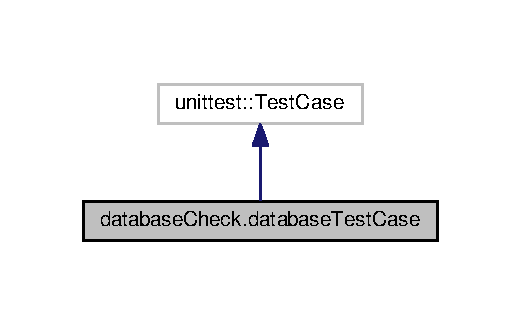
\includegraphics[width=250pt]{classdatabaseCheck_1_1databaseTestCase__inherit__graph}
\end{center}
\end{figure}


Collaboration diagram for database\+Check.\+database\+Test\+Case\+:\nopagebreak
\begin{figure}[H]
\begin{center}
\leavevmode
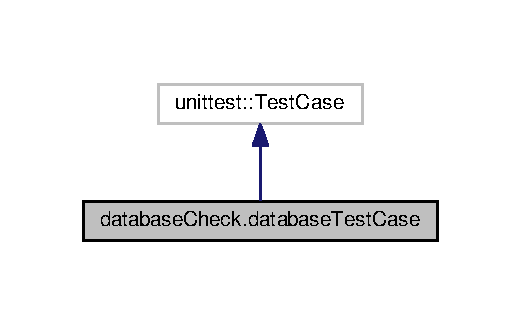
\includegraphics[width=250pt]{classdatabaseCheck_1_1databaseTestCase__coll__graph}
\end{center}
\end{figure}
\subsection*{Public Member Functions}
\begin{DoxyCompactItemize}
\item 
def \hyperlink{classdatabaseCheck_1_1databaseTestCase_a70b0175a7d4e55b8ea5129bb3c95c04b}{set\+Up\+Class} (cls)
\item 
def \hyperlink{classdatabaseCheck_1_1databaseTestCase_ac82e92d9d9ec371608937a6dc4b90e48}{tear\+Down\+Class} (cls)
\item 
def \hyperlink{classdatabaseCheck_1_1databaseTestCase_a25c2157fb4c11fb77defa664f73b3071}{set\+Up} (self)
\item 
def \hyperlink{classdatabaseCheck_1_1databaseTestCase_af1023f7bb15a9b9f2f53551957e08ebe}{tear\+Down} (self)
\item 
def \hyperlink{classdatabaseCheck_1_1databaseTestCase_ab5f77f5b303f93049ef32bbb460af468}{test\+\_\+database} (self)
\end{DoxyCompactItemize}


\subsection{Member Function Documentation}
\index{database\+Check\+::database\+Test\+Case@{database\+Check\+::database\+Test\+Case}!set\+Up@{set\+Up}}
\index{set\+Up@{set\+Up}!database\+Check\+::database\+Test\+Case@{database\+Check\+::database\+Test\+Case}}
\subsubsection[{\texorpdfstring{set\+Up(self)}{setUp(self)}}]{\setlength{\rightskip}{0pt plus 5cm}def database\+Check.\+database\+Test\+Case.\+set\+Up (
\begin{DoxyParamCaption}
\item[{}]{self}
\end{DoxyParamCaption}
)}\hypertarget{classdatabaseCheck_1_1databaseTestCase_a25c2157fb4c11fb77defa664f73b3071}{}\label{classdatabaseCheck_1_1databaseTestCase_a25c2157fb4c11fb77defa664f73b3071}
\index{database\+Check\+::database\+Test\+Case@{database\+Check\+::database\+Test\+Case}!set\+Up\+Class@{set\+Up\+Class}}
\index{set\+Up\+Class@{set\+Up\+Class}!database\+Check\+::database\+Test\+Case@{database\+Check\+::database\+Test\+Case}}
\subsubsection[{\texorpdfstring{set\+Up\+Class(cls)}{setUpClass(cls)}}]{\setlength{\rightskip}{0pt plus 5cm}def database\+Check.\+database\+Test\+Case.\+set\+Up\+Class (
\begin{DoxyParamCaption}
\item[{}]{cls}
\end{DoxyParamCaption}
)}\hypertarget{classdatabaseCheck_1_1databaseTestCase_a70b0175a7d4e55b8ea5129bb3c95c04b}{}\label{classdatabaseCheck_1_1databaseTestCase_a70b0175a7d4e55b8ea5129bb3c95c04b}
\index{database\+Check\+::database\+Test\+Case@{database\+Check\+::database\+Test\+Case}!tear\+Down@{tear\+Down}}
\index{tear\+Down@{tear\+Down}!database\+Check\+::database\+Test\+Case@{database\+Check\+::database\+Test\+Case}}
\subsubsection[{\texorpdfstring{tear\+Down(self)}{tearDown(self)}}]{\setlength{\rightskip}{0pt plus 5cm}def database\+Check.\+database\+Test\+Case.\+tear\+Down (
\begin{DoxyParamCaption}
\item[{}]{self}
\end{DoxyParamCaption}
)}\hypertarget{classdatabaseCheck_1_1databaseTestCase_af1023f7bb15a9b9f2f53551957e08ebe}{}\label{classdatabaseCheck_1_1databaseTestCase_af1023f7bb15a9b9f2f53551957e08ebe}
\index{database\+Check\+::database\+Test\+Case@{database\+Check\+::database\+Test\+Case}!tear\+Down\+Class@{tear\+Down\+Class}}
\index{tear\+Down\+Class@{tear\+Down\+Class}!database\+Check\+::database\+Test\+Case@{database\+Check\+::database\+Test\+Case}}
\subsubsection[{\texorpdfstring{tear\+Down\+Class(cls)}{tearDownClass(cls)}}]{\setlength{\rightskip}{0pt plus 5cm}def database\+Check.\+database\+Test\+Case.\+tear\+Down\+Class (
\begin{DoxyParamCaption}
\item[{}]{cls}
\end{DoxyParamCaption}
)}\hypertarget{classdatabaseCheck_1_1databaseTestCase_ac82e92d9d9ec371608937a6dc4b90e48}{}\label{classdatabaseCheck_1_1databaseTestCase_ac82e92d9d9ec371608937a6dc4b90e48}
\index{database\+Check\+::database\+Test\+Case@{database\+Check\+::database\+Test\+Case}!test\+\_\+database@{test\+\_\+database}}
\index{test\+\_\+database@{test\+\_\+database}!database\+Check\+::database\+Test\+Case@{database\+Check\+::database\+Test\+Case}}
\subsubsection[{\texorpdfstring{test\+\_\+database(self)}{test_database(self)}}]{\setlength{\rightskip}{0pt plus 5cm}def database\+Check.\+database\+Test\+Case.\+test\+\_\+database (
\begin{DoxyParamCaption}
\item[{}]{self}
\end{DoxyParamCaption}
)}\hypertarget{classdatabaseCheck_1_1databaseTestCase_ab5f77f5b303f93049ef32bbb460af468}{}\label{classdatabaseCheck_1_1databaseTestCase_ab5f77f5b303f93049ef32bbb460af468}


The documentation for this class was generated from the following file\+:\begin{DoxyCompactItemize}
\item 
Tests/\hyperlink{databaseCheck_8py}{database\+Check.\+py}\end{DoxyCompactItemize}

\hypertarget{classgetDataTest}{}\section{get\+Data\+Test Class Reference}
\label{classgetDataTest}\index{get\+Data\+Test@{get\+Data\+Test}}


Inheritance diagram for get\+Data\+Test\+:\nopagebreak
\begin{figure}[H]
\begin{center}
\leavevmode
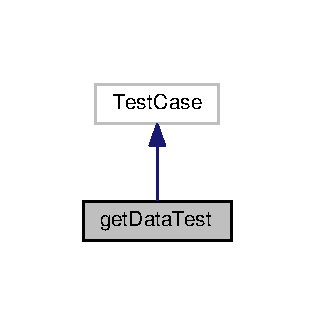
\includegraphics[width=151pt]{classgetDataTest__inherit__graph}
\end{center}
\end{figure}


Collaboration diagram for get\+Data\+Test\+:\nopagebreak
\begin{figure}[H]
\begin{center}
\leavevmode
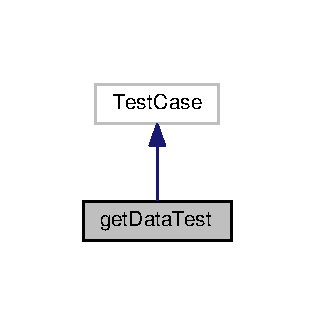
\includegraphics[width=151pt]{classgetDataTest__coll__graph}
\end{center}
\end{figure}
\subsection*{Public Member Functions}
\begin{DoxyCompactItemize}
\item 
\hyperlink{classgetDataTest_ac063fab299d53ca20bfadaa26e645901}{test\+Get\+Data} ()
\item 
\hyperlink{classgetDataTest_aa67ee4165f7d845899a511d200fad2d9}{test\+Data\+Filled} ()
\item 
\hyperlink{classgetDataTest_a62fa63cefddbaead7983efa13079dffc}{test\+Json} ()
\end{DoxyCompactItemize}


\subsection{Member Function Documentation}
\index{get\+Data\+Test@{get\+Data\+Test}!test\+Data\+Filled@{test\+Data\+Filled}}
\index{test\+Data\+Filled@{test\+Data\+Filled}!get\+Data\+Test@{get\+Data\+Test}}
\subsubsection[{\texorpdfstring{test\+Data\+Filled()}{testDataFilled()}}]{\setlength{\rightskip}{0pt plus 5cm}get\+Data\+Test\+::test\+Data\+Filled (
\begin{DoxyParamCaption}
{}
\end{DoxyParamCaption}
)}\hypertarget{classgetDataTest_aa67ee4165f7d845899a511d200fad2d9}{}\label{classgetDataTest_aa67ee4165f7d845899a511d200fad2d9}
$<$ Tests that the result has real sql data. \index{get\+Data\+Test@{get\+Data\+Test}!test\+Get\+Data@{test\+Get\+Data}}
\index{test\+Get\+Data@{test\+Get\+Data}!get\+Data\+Test@{get\+Data\+Test}}
\subsubsection[{\texorpdfstring{test\+Get\+Data()}{testGetData()}}]{\setlength{\rightskip}{0pt plus 5cm}get\+Data\+Test\+::test\+Get\+Data (
\begin{DoxyParamCaption}
{}
\end{DoxyParamCaption}
)}\hypertarget{classgetDataTest_ac063fab299d53ca20bfadaa26e645901}{}\label{classgetDataTest_ac063fab299d53ca20bfadaa26e645901}
Tests that the script returns any result \index{get\+Data\+Test@{get\+Data\+Test}!test\+Json@{test\+Json}}
\index{test\+Json@{test\+Json}!get\+Data\+Test@{get\+Data\+Test}}
\subsubsection[{\texorpdfstring{test\+Json()}{testJson()}}]{\setlength{\rightskip}{0pt plus 5cm}get\+Data\+Test\+::test\+Json (
\begin{DoxyParamCaption}
{}
\end{DoxyParamCaption}
)}\hypertarget{classgetDataTest_a62fa63cefddbaead7983efa13079dffc}{}\label{classgetDataTest_a62fa63cefddbaead7983efa13079dffc}
$<$ Tests that the data is in the right format, with non-\/null content.

$<$ check that all objects in array have full content.

!$<$ check that at least 15 entries exist 

The documentation for this class was generated from the following file\+:\begin{DoxyCompactItemize}
\item 
Tests/\hyperlink{phpTest_8php}{php\+Test.\+php}\end{DoxyCompactItemize}

\chapter{File Documentation}
\hypertarget{buildDatabase_8py}{}\section{Back/build\+Database.py File Reference}
\label{buildDatabase_8py}\index{Back/build\+Database.\+py@{Back/build\+Database.\+py}}
\subsection*{Namespaces}
\begin{DoxyCompactItemize}
\item 
 \hyperlink{namespacebuildDatabase}{build\+Database}
\end{DoxyCompactItemize}
\subsection*{Variables}
\begin{DoxyCompactItemize}
\item 
\hyperlink{namespacebuildDatabase_aeed13a096d6a186e5884c1465f8a703d}{build\+Database.\+mariadb\+\_\+connection} = mariadb.\+connect(user=\textquotesingle{}root\textquotesingle{}, password=\textquotesingle{}\textquotesingle{}, database=\textquotesingle{}csci3308\textquotesingle{}, charset=\char`\"{}utf8mb4\char`\"{})
\item 
\hyperlink{namespacebuildDatabase_ad7b3e488c85e92658c04ac329ded4206}{build\+Database.\+cursor} = mariadb\+\_\+connection.\+cursor()
\item 
\hyperlink{namespacebuildDatabase_af03183a3a08635357da39ffff3fa0c14}{build\+Database.\+secrets} = json.\+load(\hyperlink{jquery-3_8js_a9cf09a2972472098a4c689fd988f4dfc}{f})
\item 
\hyperlink{namespacebuildDatabase_ac63477d68e612f77cdca1d1adcc677da}{build\+Database.\+auth}
\item 
\hyperlink{namespacebuildDatabase_acfedb69db26209f1c7555bd335a70860}{build\+Database.\+api}
\item 
\hyperlink{namespacebuildDatabase_a0233021004fd1bc913cd8e1c81f51bdd}{build\+Database.\+trend\+Places} = api.\+trends\+\_\+available()
\item 
int \hyperlink{namespacebuildDatabase_a4ef5ab993f0509faafc01ab906cf576b}{build\+Database.\+max} = 74
\item 
\hyperlink{namespacebuildDatabase_a40723c8a3a2ff51719f1a5812af49ae2}{build\+Database.\+n\+Places} = maxiflen(trend\+Places)$>$maxelselen(trend\+Places)
\item 
\hyperlink{namespacebuildDatabase_ada15f1ae1b075d6b5385c60ad0bcba7e}{build\+Database.\+woeid} = trend\+Place\mbox{[}\textquotesingle{}woeid\textquotesingle{}\mbox{]}
\item 
\hyperlink{namespacebuildDatabase_a2d66916cea7965a5f65dd98ef44dd261}{build\+Database.\+city} = trend\+Place\mbox{[}\textquotesingle{}name\textquotesingle{}\mbox{]}
\item 
\hyperlink{namespacebuildDatabase_a0d6b3715d584e19547cb25cd7f0f4d28}{build\+Database.\+query\+City} = cursor.\+execute(\char`\"{}S\+E\+L\+E\+CT Lat,Lng F\+R\+OM \hyperlink{initMapScript_8js_a76167830814420bde81accf9e460aa96}{cities} W\+H\+E\+RE \hyperlink{classCity}{City} = \textquotesingle{}\char`\"{} + city+\char`\"{}\textquotesingle{};\char`\"{})
\item 
\hyperlink{namespacebuildDatabase_ad2781a91cbfcd21e5be44aae5d39d257}{build\+Database.\+location} = cursor.\+fetchone()
\item 
string \hyperlink{namespacebuildDatabase_ac6de86e53e5b1e858c4bfc30606561e0}{build\+Database.\+geocode} = str(location\mbox{[}0\mbox{]})+\char`\"{},\char`\"{}
\item 
\hyperlink{namespacebuildDatabase_a00e15f8c5a38ef71e1176db990041ee0}{build\+Database.\+trends} = api.\+trends\+\_\+place(woeid)\mbox{[}0\mbox{]}\mbox{[}\textquotesingle{}trends\textquotesingle{}\mbox{]}
\item 
int \hyperlink{namespacebuildDatabase_a1a68c0e0f8d22d281ad1a8b9024fd5d1}{build\+Database.\+largest} = -\/1
\item 
int \hyperlink{namespacebuildDatabase_abfd839e1a537e9e0ca132979eee02a28}{build\+Database.\+largest\+Ind} = -\/1
\item 
\hyperlink{namespacebuildDatabase_afe0b1b9174b6ce79a6fca681db02d2c6}{build\+Database.\+trend} = trends\mbox{[}largest\+Ind\mbox{]}
\item 
\hyperlink{namespacebuildDatabase_a41e7e514b01675f060ab36db44904a13}{build\+Database.\+tweets} = tweepy.\+Cursor(api.\+search, \hyperlink{jquery-3_8js_aee3046c01d22ccd1efcb944608aec125}{q}=trend\mbox{[}\textquotesingle{}query\textquotesingle{}\mbox{]}, geocode=geocode).items(99)
\item 
string \hyperlink{namespacebuildDatabase_a6b90ef6e990c311046eeaed437c20194}{build\+Database.\+tweet\+Texts} = \textquotesingle{}\textquotesingle{}
\item 
int \hyperlink{namespacebuildDatabase_a50f9b6bae964e6579ba92450127cf440}{build\+Database.\+most\+Positive} = \mbox{[}(-\/2, \textquotesingle{}\textquotesingle{})\mbox{]}$\ast$5
\item 
int \hyperlink{namespacebuildDatabase_adee8ced6b5216c8ebe3ad73fb6b9eb9a}{build\+Database.\+most\+Negative} = \mbox{[}(2, \textquotesingle{}\textquotesingle{})\mbox{]}$\ast$5
\item 
\hyperlink{namespacebuildDatabase_ad338d82c1c3c6c3d5df5034a51af3503}{build\+Database.\+text} = tweet.\+text
\item 
\hyperlink{namespacebuildDatabase_ab8145fb3b51cc107e9f177ffe6b4ab29}{build\+Database.\+sent} = Text\+Blob(text).sentiment.\+polarity
\item 
bool \hyperlink{namespacebuildDatabase_ab9d82862a48f7e4e725a899047b7ee75}{build\+Database.\+inserted} = False
\item 
\hyperlink{namespacebuildDatabase_a05391cf14f340a054d4f2c708576be29}{build\+Database.\+blob} = Text\+Blob(tweet\+Texts)
\end{DoxyCompactItemize}

\hypertarget{storeCities_8py}{}\section{Back/store\+Cities.py File Reference}
\label{storeCities_8py}\index{Back/store\+Cities.\+py@{Back/store\+Cities.\+py}}
\subsection*{Namespaces}
\begin{DoxyCompactItemize}
\item 
 \hyperlink{namespacestoreCities}{store\+Cities}
\end{DoxyCompactItemize}
\subsection*{Variables}
\begin{DoxyCompactItemize}
\item 
\hyperlink{namespacestoreCities_a8f8c246ff77d060c8069df768b152c49}{store\+Cities.\+mariadb\+\_\+connection} = mariadb.\+connect(user = \textquotesingle{}root\textquotesingle{}, password = \textquotesingle{}\textquotesingle{}, database=\textquotesingle{}csci3308\textquotesingle{})
\item 
\hyperlink{namespacestoreCities_a646bdebfa2acb2fc972c5ad8432a1b77}{store\+Cities.\+cursor} = mariadb\+\_\+connection.\+cursor()
\item 
\hyperlink{namespacestoreCities_a7b9da38e052d859e8c0dcc3ab0c8948c}{store\+Cities.\+tweets} = cursor.\+fetchall()
\item 
\hyperlink{namespacestoreCities_a49f77864c3f28f848d31dfc26ab2a9a4}{store\+Cities.\+city} = tweet\mbox{[}0\mbox{]}
\item 
\hyperlink{namespacestoreCities_abb67378575f786533b2e9e00137c0c11}{store\+Cities.\+lat} = tweet\mbox{[}1\mbox{]}
\item 
\hyperlink{namespacestoreCities_a991d2b6bd50ff73a116167b0ec2fb252}{store\+Cities.\+lng} = tweet\mbox{[}2\mbox{]}
\end{DoxyCompactItemize}

\hypertarget{bootstrap_8js}{}\section{Front/bootstrap.js File Reference}
\label{bootstrap_8js}\index{Front/bootstrap.\+js@{Front/bootstrap.\+js}}
\subsection*{Functions}
\begin{DoxyCompactItemize}
\item 
\hyperlink{bootstrap_8js_aa2bdb854ead8cc8b8018b1e7f536e543}{!function} (\hyperlink{popper_8js_a23c5666e83bbbceee94adcd0851f50c4}{t}, \hyperlink{popper_8js_a2c038346d47955cbe2cb91e338edd7e1}{e})
\item 
function \hyperlink{bootstrap_8js_a73aff07b65d7c0b09ccf6b4c4f1b7a9d}{i} (\hyperlink{popper_8js_a23c5666e83bbbceee94adcd0851f50c4}{t}, \hyperlink{popper_8js_a2c038346d47955cbe2cb91e338edd7e1}{e})
\item 
function \hyperlink{bootstrap_8js_ae1f57cfe393e1e182cf26e0346a0ba28}{s} (\hyperlink{popper_8js_a23c5666e83bbbceee94adcd0851f50c4}{t}, \hyperlink{popper_8js_a2c038346d47955cbe2cb91e338edd7e1}{e}, \hyperlink{jquery-3_8js_a3c7365c007156a2a63223e3c9909fbf8}{n})
\item 
function \hyperlink{bootstrap_8js_a1e99b66ec05f848b367484f62b1d1521}{r} ()
\item 
\hyperlink{bootstrap_8js_a6e2c9a4472a75ae2ec32ee54ff87c001}{!function} (\hyperlink{popper_8js_a23c5666e83bbbceee94adcd0851f50c4}{t})
\item 
\hyperlink{popper_8js_a23c5666e83bbbceee94adcd0851f50c4}{t} \hyperlink{popper_8js_a23c5666e83bbbceee94adcd0851f50c4}{t} \hyperlink{popper_8js_a23c5666e83bbbceee94adcd0851f50c4}{t} \hyperlink{popper_8js_a23c5666e83bbbceee94adcd0851f50c4}{t} \hyperlink{popper_8js_a23c5666e83bbbceee94adcd0851f50c4}{t} \hyperlink{popper_8js_a23c5666e83bbbceee94adcd0851f50c4}{t} \hyperlink{popper_8js_a23c5666e83bbbceee94adcd0851f50c4}{t} \hyperlink{popper_8js_a23c5666e83bbbceee94adcd0851f50c4}{t} \hyperlink{popper_8js_a23c5666e83bbbceee94adcd0851f50c4}{t} \hyperlink{popper_8js_a23c5666e83bbbceee94adcd0851f50c4}{t} \hyperlink{popper_8js_a23c5666e83bbbceee94adcd0851f50c4}{t} Object \hyperlink{bootstrap_8js_a677f3f43ddb2b0c3d869973e9c157184}{define\+Property} (\hyperlink{popper_8js_a23c5666e83bbbceee94adcd0851f50c4}{t},\char`\"{}\+\_\+\+\_\+es\+Module\char`\"{},\{value\+:!0\})\})
\end{DoxyCompactItemize}
\subsection*{Variables}
\begin{DoxyCompactItemize}
\item 
\hyperlink{bootstrap_8js_a05c09a5e9d53fa7adf0a7936038c2fa3}{this}
\item 
function \hyperlink{bootstrap_8js_a23c5666e83bbbceee94adcd0851f50c4}{t}
\item 
function \hyperlink{bootstrap_8js_a08a4415e9d594ff960030b921d42b91e}{e} =e\&\&e.\+has\+Own\+Property(\char`\"{}default\char`\"{})?e.\+default\+:e
\item 
function \hyperlink{bootstrap_8js_aeab71244afb687f16d8c4f5ee9d6ef0e}{n} \{\char`\"{}use strict\char`\"{}
\item 
var \hyperlink{bootstrap_8js_a400dc8109620963da8314d4bdfa14f83}{o}
\item 
var \hyperlink{bootstrap_8js_a82ca4ee5dd63e58a2bb967077dc8b8fb}{a}
\item 
var \hyperlink{bootstrap_8js_ae5e71a2600e8891c54854be157cc6626}{l}
\item 
var \hyperlink{bootstrap_8js_a79fe0eb780a2a4b5543b4dddf8b6188a}{h}
\item 
var \hyperlink{bootstrap_8js_abce695e0af988ece0826d9ad59b8160d}{c}
\item 
var \hyperlink{bootstrap_8js_accb4ce8dd4113ac0f510653e31809106}{u}
\item 
var \hyperlink{bootstrap_8js_a9cf09a2972472098a4c689fd988f4dfc}{f}
\item 
var \hyperlink{bootstrap_8js_aeb337d295abaddb5ec3cb34cc2e2bbc9}{d}
\item 
var \hyperlink{bootstrap_8js_a6e69a5af94d7d53886e51f89fb3bd6b4}{\+\_\+}
\item 
var \hyperlink{bootstrap_8js_a103df269476e78897c9c4c6cb8f4eb06}{g}
\item 
var \hyperlink{bootstrap_8js_ad1707b001240e9c8298830073364c8bf}{p}
\item 
var \hyperlink{bootstrap_8js_a9e77e016b2928d7dcb493b89a0c9dc32}{m}
\item 
var \hyperlink{bootstrap_8js_afc3dd12de12777f6e20b4c93b7e7cb96}{v}
\item 
var \hyperlink{bootstrap_8js_ae406f8d6be3dab2e4d9b41c963380c36}{E}
\item 
var \hyperlink{bootstrap_8js_aa798e0c32253f973f3154aa30c996eb2}{T}
\item 
var \hyperlink{bootstrap_8js_a0b31909b1cae9ed1db6ff042057fce60}{y}
\item 
var \hyperlink{bootstrap_8js_ae59e0ac8d0c43c81f50236f719763efc}{C}
\item 
var \hyperlink{bootstrap_8js_aeaf7b778b1c5115bbe67bc6c0a472011}{I}
\item 
var \hyperlink{bootstrap_8js_a9757042cb6157b0f84e78a5ff4aa6f93}{A}
\item 
var \hyperlink{bootstrap_8js_aa4026ad5544b958e54ce5e106fa1c805}{b}
\item 
var \hyperlink{bootstrap_8js_ad741d7cd7e6eda75030b55e36b706c0a}{D}
\item 
var \hyperlink{bootstrap_8js_a8bab16140cede5f71c657e8dc46c1887}{S}
\item 
var \hyperlink{bootstrap_8js_a9721a992655f700bdc2e91ba68b71e26}{w}
\item 
var \hyperlink{bootstrap_8js_abadc8a6494eb0561422367930ee2c126}{N}
\item 
var \hyperlink{bootstrap_8js_a351d74368c902b5870c03ff2d1683f30}{O}
\item 
var \hyperlink{bootstrap_8js_ab26645c014aa005ecedef329ecf58c99}{k}
\item 
var \hyperlink{bootstrap_8js_a5f11e71574d0fa4e61140f70fd15f3cd}{P} =function(\hyperlink{popper_8js_a23c5666e83bbbceee94adcd0851f50c4}{t})\{var \hyperlink{popper_8js_a2c038346d47955cbe2cb91e338edd7e1}{e}=!1;function \hyperlink{jquery-3_8js_a3c7365c007156a2a63223e3c9909fbf8}{n}(\hyperlink{popper_8js_a2c038346d47955cbe2cb91e338edd7e1}{e})\{var \hyperlink{jquery-3_8js_a3c7365c007156a2a63223e3c9909fbf8}{n}=\hyperlink{bootstrap_8js_a05c09a5e9d53fa7adf0a7936038c2fa3}{this},\hyperlink{bootstrap_8js_ae1f57cfe393e1e182cf26e0346a0ba28}{s}=!1;return \hyperlink{popper_8js_a23c5666e83bbbceee94adcd0851f50c4}{t}(\hyperlink{bootstrap_8js_a05c09a5e9d53fa7adf0a7936038c2fa3}{this}).one(i.\+T\+R\+A\+N\+S\+I\+T\+I\+O\+N\+\_\+\+E\+ND,function()\{\hyperlink{bootstrap_8js_ae1f57cfe393e1e182cf26e0346a0ba28}{s}=!0\}),set\+Timeout(function()\{\hyperlink{bootstrap_8js_ae1f57cfe393e1e182cf26e0346a0ba28}{s}$\vert$$\vert$i.\+trigger\+Transition\+End(\hyperlink{jquery-3_8js_a3c7365c007156a2a63223e3c9909fbf8}{n})\},\hyperlink{popper_8js_a2c038346d47955cbe2cb91e338edd7e1}{e}),\hyperlink{bootstrap_8js_a05c09a5e9d53fa7adf0a7936038c2fa3}{this}\}var \hyperlink{bootstrap_8js_a73aff07b65d7c0b09ccf6b4c4f1b7a9d}{i}=\{T\+R\+A\+N\+S\+I\+T\+I\+O\+N\+\_\+\+E\+N\+D\+:\char`\"{}bs\+Transition\+End\char`\"{},get\+U\+I\+D\+:function(\hyperlink{popper_8js_a23c5666e83bbbceee94adcd0851f50c4}{t})\{do\{\hyperlink{popper_8js_a23c5666e83bbbceee94adcd0851f50c4}{t}+=$\sim$$\sim$(1e6$\ast$\+Math.\+random())\}while(document.\+get\+Element\+By\+Id(t));return t\},get\+Selector\+From\+Element\+:function(e)\{var n,i=e.\+get\+Attribute(\char`\"{}data-\/target\char`\"{});i\&\&\char`\"{}\#\char`\"{}!==i$\vert$$\vert$(i=e.\+get\+Attribute(\char`\"{}href\char`\"{})$\vert$$\vert$\char`\"{}\char`\"{}),\char`\"{}\#\char`\"{}===i.\+char\+At(0)\&\&(n=i,i=n=\char`\"{}function\char`\"{}==typeof t.\+escape\+Selector?t.\+escape\+Selector(n).\+substr(1)\+:n.\+replace(/(\+:$\vert$\textbackslash{}.$\vert$\textbackslash{}\mbox{[}$\vert$\textbackslash{}\mbox{]}$\vert$,$\vert$=$\vert$@)/g,\char`\"{}\textbackslash{}\textbackslash{}\$1\char`\"{}));try\{return t(document).\+find(i).\+length$>$0?i\+:null\}catch(t)\{return null\}\},reflow\+:function(t)\{return t.\+offset\+Height\},trigger\+Transition\+End\+:function(n)\{t(n).\+trigger(e.\+end)\},supports\+Transition\+End\+:function()\{return Boolean(e)\},is\+Element\+:function(t)\{return(t\mbox{[}0\mbox{]}$\vert$$\vert$t).\+node\+Type\},type\+Check\+Config\+:function(t,e,n)\{for(var s in n)if(\+Object.\+prototype.\+has\+Own\+Property.\+call(n,s))\{var r=n\mbox{[}s\mbox{]},o=e\mbox{[}s\mbox{]},a=o\&\&i.\+is\+Element(o)?\char`\"{}element\char`\"{}\+:(l=o,\{\}.\+to\+String.\+call(l).\+match(/\textbackslash{}s(\mbox{[}a-\/z\+A-\/\+Z\mbox{]}+)/)\mbox{[}1\mbox{]}.\+to\+Lower\+Case());if(!new Reg\+Exp(r).\+test(a))throw new Error(t.\+to\+Upper\+Case()+\textquotesingle{}\+: Option \char`\"{}\textquotesingle{}+s+\textquotesingle{}\char`\"{} provided type \char`\"{}\textquotesingle{}+a+\textquotesingle{}\char`\"{} but expected type \char`\"{}\textquotesingle{}+r+\textquotesingle{}\char`\"{}.\textquotesingle{})\}var l\}\};return e=(\char`\"{}undefined\char`\"{}==typeof window$\vert$$\vert$!window.\+Q\+Unit)\&\&\{end\+:\char`\"{}transitionend\char`\"{}\},t.\+fn.\+emulate\+Transition\+End=n,i.\+supports\+Transition\+End()\&\&(t.\+event.\+special\mbox{[}i.\+T\+R\+A\+N\+S\+I\+T\+I\+O\+N\+\_\+\+E\+N\+D\mbox{]}=\{bind\+Type\+:e.\+end,delegate\+Type\+:e.\+end,handle\+:function(e)\{if(t(e.\+target).\+is(this))return e.\+handle\+Obj.\+handler.\+apply(this,arguments)\}\}),i\}(e)
\item 
var \hyperlink{bootstrap_8js_af17802630779ec5087c1028d57f3d02b}{L} =(\hyperlink{jquery-3_8js_aa4d4888597588a84fd5b1184d00c91f3}{a}=\char`\"{}alert\char`\"{},h=\char`\"{}.\char`\"{}+(\hyperlink{jquery-3_8js_ae5e71a2600e8891c54854be157cc6626}{l}=\char`\"{}bs.\+alert\char`\"{}),c=(\hyperlink{jquery-3_8js_a400dc8109620963da8314d4bdfa14f83}{o}=\hyperlink{popper_8js_a2c038346d47955cbe2cb91e338edd7e1}{e}).\hyperlink{jquery-3_8js_abf890a0227732ad023a253e8c19e0660}{fn}\mbox{[}\hyperlink{jquery-3_8js_aa4d4888597588a84fd5b1184d00c91f3}{a}\mbox{]},\hyperlink{jquery-3_8js_accb4ce8dd4113ac0f510653e31809106}{u}=\{C\+L\+O\+S\+E\+:\char`\"{}close\char`\"{}+h,C\+L\+O\+S\+E\+D\+:\char`\"{}closed\char`\"{}+h,C\+L\+I\+C\+K\+\_\+\+D\+A\+T\+A\+\_\+\+A\+P\+I\+:\char`\"{}click\char`\"{}+h+\char`\"{}.data-\/api\char`\"{}\},f=\char`\"{}alert\char`\"{},d=\char`\"{}fade\char`\"{},\+\_\+=\char`\"{}show\char`\"{},g=function()\{function \hyperlink{popper_8js_a23c5666e83bbbceee94adcd0851f50c4}{t}(\hyperlink{popper_8js_a23c5666e83bbbceee94adcd0851f50c4}{t})\{this.\+\_\+element=\hyperlink{popper_8js_a23c5666e83bbbceee94adcd0851f50c4}{t}\}var \hyperlink{popper_8js_a2c038346d47955cbe2cb91e338edd7e1}{e}=t.\+prototype;return e.\+close=function(\hyperlink{popper_8js_a23c5666e83bbbceee94adcd0851f50c4}{t})\{\hyperlink{popper_8js_a23c5666e83bbbceee94adcd0851f50c4}{t}=\hyperlink{popper_8js_a23c5666e83bbbceee94adcd0851f50c4}{t}$\vert$$\vert$this.\+\_\+element;var \hyperlink{popper_8js_a2c038346d47955cbe2cb91e338edd7e1}{e}=this.\+\_\+get\+Root\+Element(\hyperlink{popper_8js_a23c5666e83bbbceee94adcd0851f50c4}{t});this.\+\_\+trigger\+Close\+Event(\hyperlink{popper_8js_a2c038346d47955cbe2cb91e338edd7e1}{e}).is\+Default\+Prevented()$\vert$$\vert$this.\+\_\+remove\+Element(\hyperlink{popper_8js_a2c038346d47955cbe2cb91e338edd7e1}{e})\},e.\+dispose=function()\{o.\+remove\+Data(this.\+\_\+element,\hyperlink{jquery-3_8js_ae5e71a2600e8891c54854be157cc6626}{l}),this.\+\_\+element=null\},e.\+\_\+get\+Root\+Element=function(\hyperlink{popper_8js_a23c5666e83bbbceee94adcd0851f50c4}{t})\{var \hyperlink{popper_8js_a2c038346d47955cbe2cb91e338edd7e1}{e}=P.\+get\+Selector\+From\+Element(\hyperlink{popper_8js_a23c5666e83bbbceee94adcd0851f50c4}{t}),\hyperlink{jquery-3_8js_a3c7365c007156a2a63223e3c9909fbf8}{n}=!1;return \hyperlink{popper_8js_a2c038346d47955cbe2cb91e338edd7e1}{e}\&\&(\hyperlink{jquery-3_8js_a3c7365c007156a2a63223e3c9909fbf8}{n}=\hyperlink{jquery-3_8js_a400dc8109620963da8314d4bdfa14f83}{o}(\hyperlink{popper_8js_a2c038346d47955cbe2cb91e338edd7e1}{e})\mbox{[}0\mbox{]}),\hyperlink{jquery-3_8js_a3c7365c007156a2a63223e3c9909fbf8}{n}$\vert$$\vert$(\hyperlink{jquery-3_8js_a3c7365c007156a2a63223e3c9909fbf8}{n}=\hyperlink{jquery-3_8js_a400dc8109620963da8314d4bdfa14f83}{o}(\hyperlink{popper_8js_a23c5666e83bbbceee94adcd0851f50c4}{t}).closest(\char`\"{}.\char`\"{}+\hyperlink{jquery-3_8js_a9cf09a2972472098a4c689fd988f4dfc}{f})\mbox{[}0\mbox{]}),\hyperlink{jquery-3_8js_a3c7365c007156a2a63223e3c9909fbf8}{n}\},e.\+\_\+trigger\+Close\+Event=function(\hyperlink{popper_8js_a23c5666e83bbbceee94adcd0851f50c4}{t})\{var \hyperlink{popper_8js_a2c038346d47955cbe2cb91e338edd7e1}{e}=o.\+Event(u.\+C\+L\+O\+SE);return \hyperlink{jquery-3_8js_a400dc8109620963da8314d4bdfa14f83}{o}(\hyperlink{popper_8js_a23c5666e83bbbceee94adcd0851f50c4}{t}).trigger(\hyperlink{popper_8js_a2c038346d47955cbe2cb91e338edd7e1}{e}),\hyperlink{popper_8js_a2c038346d47955cbe2cb91e338edd7e1}{e}\},e.\+\_\+remove\+Element=function(\hyperlink{popper_8js_a23c5666e83bbbceee94adcd0851f50c4}{t})\{var \hyperlink{popper_8js_a2c038346d47955cbe2cb91e338edd7e1}{e}=\hyperlink{bootstrap_8js_a05c09a5e9d53fa7adf0a7936038c2fa3}{this};\hyperlink{jquery-3_8js_a400dc8109620963da8314d4bdfa14f83}{o}(\hyperlink{popper_8js_a23c5666e83bbbceee94adcd0851f50c4}{t}).remove\+Class(\hyperlink{bootstrap_8js_a6e69a5af94d7d53886e51f89fb3bd6b4}{\+\_\+}),P.\+supports\+Transition\+End()\&\&\hyperlink{jquery-3_8js_a400dc8109620963da8314d4bdfa14f83}{o}(\hyperlink{popper_8js_a23c5666e83bbbceee94adcd0851f50c4}{t}).has\+Class(\hyperlink{jquery-3_8js_aeb337d295abaddb5ec3cb34cc2e2bbc9}{d})?\hyperlink{jquery-3_8js_a400dc8109620963da8314d4bdfa14f83}{o}(\hyperlink{popper_8js_a23c5666e83bbbceee94adcd0851f50c4}{t}).one(P.\+T\+R\+A\+N\+S\+I\+T\+I\+O\+N\+\_\+\+E\+ND,function(\hyperlink{jquery-3_8js_a3c7365c007156a2a63223e3c9909fbf8}{n})\{return e.\+\_\+destroy\+Element(\hyperlink{popper_8js_a23c5666e83bbbceee94adcd0851f50c4}{t},\hyperlink{jquery-3_8js_a3c7365c007156a2a63223e3c9909fbf8}{n})\}).emulate\+Transition\+End(150)\+:this.\+\_\+destroy\+Element(\hyperlink{popper_8js_a23c5666e83bbbceee94adcd0851f50c4}{t})\},e.\+\_\+destroy\+Element=function(\hyperlink{popper_8js_a23c5666e83bbbceee94adcd0851f50c4}{t})\{\hyperlink{jquery-3_8js_a400dc8109620963da8314d4bdfa14f83}{o}(\hyperlink{popper_8js_a23c5666e83bbbceee94adcd0851f50c4}{t}).detach().trigger(u.\+C\+L\+O\+S\+ED).remove()\},t.\+\_\+j\+Query\+Interface=function(\hyperlink{popper_8js_a2c038346d47955cbe2cb91e338edd7e1}{e})\{return \hyperlink{jquery-3_8js_a15d8398b77829795291db9587eaa2e94}{this.\+each}(function()\{var \hyperlink{jquery-3_8js_a3c7365c007156a2a63223e3c9909fbf8}{n}=\hyperlink{jquery-3_8js_a400dc8109620963da8314d4bdfa14f83}{o}(\hyperlink{bootstrap_8js_a05c09a5e9d53fa7adf0a7936038c2fa3}{this}),\hyperlink{bootstrap_8js_a73aff07b65d7c0b09ccf6b4c4f1b7a9d}{i}=n.\+data(\hyperlink{jquery-3_8js_ae5e71a2600e8891c54854be157cc6626}{l});\hyperlink{bootstrap_8js_a73aff07b65d7c0b09ccf6b4c4f1b7a9d}{i}$\vert$$\vert$(\hyperlink{bootstrap_8js_a73aff07b65d7c0b09ccf6b4c4f1b7a9d}{i}=new \hyperlink{popper_8js_a23c5666e83bbbceee94adcd0851f50c4}{t}(\hyperlink{bootstrap_8js_a05c09a5e9d53fa7adf0a7936038c2fa3}{this}),n.\+data(\hyperlink{jquery-3_8js_ae5e71a2600e8891c54854be157cc6626}{l},\hyperlink{bootstrap_8js_a73aff07b65d7c0b09ccf6b4c4f1b7a9d}{i})),\char`\"{}close\char`\"{}===e\&\&\hyperlink{bootstrap_8js_a73aff07b65d7c0b09ccf6b4c4f1b7a9d}{i}\mbox{[}\hyperlink{popper_8js_a2c038346d47955cbe2cb91e338edd7e1}{e}\mbox{]}(\hyperlink{bootstrap_8js_a05c09a5e9d53fa7adf0a7936038c2fa3}{this})\})\},t.\+\_\+handle\+Dismiss=function(\hyperlink{popper_8js_a23c5666e83bbbceee94adcd0851f50c4}{t})\{return function(\hyperlink{popper_8js_a2c038346d47955cbe2cb91e338edd7e1}{e})\{\hyperlink{popper_8js_a2c038346d47955cbe2cb91e338edd7e1}{e}\&\&e.\+prevent\+Default(),t.\+close(\hyperlink{bootstrap_8js_a05c09a5e9d53fa7adf0a7936038c2fa3}{this})\}\},\hyperlink{bootstrap_8js_ae1f57cfe393e1e182cf26e0346a0ba28}{s}(\hyperlink{popper_8js_a23c5666e83bbbceee94adcd0851f50c4}{t},null,\mbox{[}\{key\+:\char`\"{}V\+E\+R\+S\+I\+ON\char`\"{},get\+:function()\{return\char`\"{}4.\+0.\+0\char`\"{}\}\}\mbox{]}),\hyperlink{popper_8js_a23c5666e83bbbceee94adcd0851f50c4}{t}\}(),\hyperlink{jquery-3_8js_a400dc8109620963da8314d4bdfa14f83}{o}(document).on(u.\+C\+L\+I\+C\+K\+\_\+\+D\+A\+T\+A\+\_\+\+A\+PI,\textquotesingle{}\mbox{[}data-\/dismiss=\char`\"{}alert\char`\"{}\mbox{]}\textquotesingle{},g.\+\_\+handle\+Dismiss(new \hyperlink{jquery-3_8js_a103df269476e78897c9c4c6cb8f4eb06}{g})),\hyperlink{jquery-3_8js_abf890a0227732ad023a253e8c19e0660}{o.\+fn}\mbox{[}\hyperlink{jquery-3_8js_aa4d4888597588a84fd5b1184d00c91f3}{a}\mbox{]}=g.\+\_\+j\+Query\+Interface,\hyperlink{jquery-3_8js_abf890a0227732ad023a253e8c19e0660}{o.\+fn}\mbox{[}\hyperlink{jquery-3_8js_aa4d4888597588a84fd5b1184d00c91f3}{a}\mbox{]}.Constructor=\hyperlink{jquery-3_8js_a103df269476e78897c9c4c6cb8f4eb06}{g},\hyperlink{jquery-3_8js_abf890a0227732ad023a253e8c19e0660}{o.\+fn}\mbox{[}\hyperlink{jquery-3_8js_aa4d4888597588a84fd5b1184d00c91f3}{a}\mbox{]}.no\+Conflict=function()\{return \hyperlink{jquery-3_8js_abf890a0227732ad023a253e8c19e0660}{o.\+fn}\mbox{[}\hyperlink{jquery-3_8js_aa4d4888597588a84fd5b1184d00c91f3}{a}\mbox{]}=\hyperlink{jquery-3_8js_abce695e0af988ece0826d9ad59b8160d}{c},g.\+\_\+j\+Query\+Interface\},\hyperlink{jquery-3_8js_a103df269476e78897c9c4c6cb8f4eb06}{g})
\item 
var \hyperlink{bootstrap_8js_a09083e327c397ffc75bdc32d72212c70}{R} =(\hyperlink{jquery-3_8js_a9e77e016b2928d7dcb493b89a0c9dc32}{m}=\char`\"{}button\char`\"{},E=\char`\"{}.\char`\"{}+(\hyperlink{jquery-3_8js_afc3dd12de12777f6e20b4c93b7e7cb96}{v}=\char`\"{}bs.\+button\char`\"{}),T=\char`\"{}.data-\/api\char`\"{},y=(\hyperlink{jquery-3_8js_ae314c6c724250fd29b7ca94473145cef}{p}=\hyperlink{popper_8js_a2c038346d47955cbe2cb91e338edd7e1}{e}).\hyperlink{jquery-3_8js_abf890a0227732ad023a253e8c19e0660}{fn}\mbox{[}\hyperlink{jquery-3_8js_a9e77e016b2928d7dcb493b89a0c9dc32}{m}\mbox{]},\hyperlink{bootstrap_8js_ae59e0ac8d0c43c81f50236f719763efc}{C}=\char`\"{}active\char`\"{},I=\char`\"{}btn\char`\"{},A=\char`\"{}focus\char`\"{},b=\textquotesingle{}\mbox{[}data-\/toggle$^\wedge$=\char`\"{}button\char`\"{}\mbox{]}\textquotesingle{},D=\textquotesingle{}\mbox{[}data-\/toggle=\char`\"{}buttons\char`\"{}\mbox{]}\textquotesingle{},S=\char`\"{}input\char`\"{},w=\char`\"{}.active\char`\"{},N=\char`\"{}.btn\char`\"{},O=\{C\+L\+I\+C\+K\+\_\+\+D\+A\+T\+A\+\_\+\+A\+P\+I\+:\char`\"{}click\char`\"{}+E+\hyperlink{bootstrap_8js_aa798e0c32253f973f3154aa30c996eb2}{T},F\+O\+C\+U\+S\+\_\+\+B\+L\+U\+R\+\_\+\+D\+A\+T\+A\+\_\+\+A\+P\+I\+:\char`\"{}focus\char`\"{}+E+\hyperlink{bootstrap_8js_aa798e0c32253f973f3154aa30c996eb2}{T}+\char`\"{} blur\char`\"{}+E+\hyperlink{bootstrap_8js_aa798e0c32253f973f3154aa30c996eb2}{T}\},\hyperlink{jquery-3_8js_ab26645c014aa005ecedef329ecf58c99}{k}=function()\{function \hyperlink{popper_8js_a23c5666e83bbbceee94adcd0851f50c4}{t}(\hyperlink{popper_8js_a23c5666e83bbbceee94adcd0851f50c4}{t})\{this.\+\_\+element=\hyperlink{popper_8js_a23c5666e83bbbceee94adcd0851f50c4}{t}\}var \hyperlink{popper_8js_a2c038346d47955cbe2cb91e338edd7e1}{e}=t.\+prototype;return e.\+toggle=function()\{var \hyperlink{popper_8js_a23c5666e83bbbceee94adcd0851f50c4}{t}=!0,\hyperlink{popper_8js_a2c038346d47955cbe2cb91e338edd7e1}{e}=!0,\hyperlink{jquery-3_8js_a3c7365c007156a2a63223e3c9909fbf8}{n}=\hyperlink{jquery-3_8js_ae314c6c724250fd29b7ca94473145cef}{p}(this.\+\_\+element).closest(\hyperlink{bootstrap_8js_ad741d7cd7e6eda75030b55e36b706c0a}{D})\mbox{[}0\mbox{]};if(\hyperlink{jquery-3_8js_a3c7365c007156a2a63223e3c9909fbf8}{n})\{var \hyperlink{bootstrap_8js_a73aff07b65d7c0b09ccf6b4c4f1b7a9d}{i}=\hyperlink{jquery-3_8js_ae314c6c724250fd29b7ca94473145cef}{p}(this.\+\_\+element).find(\hyperlink{bootstrap_8js_a8bab16140cede5f71c657e8dc46c1887}{S})\mbox{[}0\mbox{]};if(\hyperlink{bootstrap_8js_a73aff07b65d7c0b09ccf6b4c4f1b7a9d}{i})\{if(\char`\"{}radio\char`\"{}===i.\+type)if(i.\+checked\&\&\hyperlink{jquery-3_8js_ae314c6c724250fd29b7ca94473145cef}{p}(this.\+\_\+element).has\+Class(\hyperlink{bootstrap_8js_ae59e0ac8d0c43c81f50236f719763efc}{C}))\hyperlink{popper_8js_a23c5666e83bbbceee94adcd0851f50c4}{t}=!1;else\{var \hyperlink{bootstrap_8js_ae1f57cfe393e1e182cf26e0346a0ba28}{s}=\hyperlink{jquery-3_8js_ae314c6c724250fd29b7ca94473145cef}{p}(\hyperlink{jquery-3_8js_a3c7365c007156a2a63223e3c9909fbf8}{n}).find(\hyperlink{jquery-3_8js_a9e7acde64afa4ba72de6fa724a96c17a}{w})\mbox{[}0\mbox{]};\hyperlink{bootstrap_8js_ae1f57cfe393e1e182cf26e0346a0ba28}{s}\&\&\hyperlink{jquery-3_8js_ae314c6c724250fd29b7ca94473145cef}{p}(\hyperlink{bootstrap_8js_ae1f57cfe393e1e182cf26e0346a0ba28}{s}).remove\+Class(\hyperlink{bootstrap_8js_ae59e0ac8d0c43c81f50236f719763efc}{C})\}if(\hyperlink{popper_8js_a23c5666e83bbbceee94adcd0851f50c4}{t})\{if(i.\+has\+Attribute(\char`\"{}disabled\char`\"{})$\vert$$\vert$n.\+has\+Attribute(\char`\"{}disabled\char`\"{})$\vert$$\vert$i.\+class\+List.\+contains(\char`\"{}disabled\char`\"{})$\vert$$\vert$n.\+class\+List.\+contains(\char`\"{}disabled\char`\"{}))return;i.\+checked=!\hyperlink{jquery-3_8js_ae314c6c724250fd29b7ca94473145cef}{p}(this.\+\_\+element).has\+Class(\hyperlink{bootstrap_8js_ae59e0ac8d0c43c81f50236f719763efc}{C}),\hyperlink{jquery-3_8js_ae314c6c724250fd29b7ca94473145cef}{p}(\hyperlink{bootstrap_8js_a73aff07b65d7c0b09ccf6b4c4f1b7a9d}{i}).trigger(\char`\"{}change\char`\"{})\}i.\+focus(),\hyperlink{popper_8js_a2c038346d47955cbe2cb91e338edd7e1}{e}=!1\}\}\hyperlink{popper_8js_a2c038346d47955cbe2cb91e338edd7e1}{e}\&\&this.\+\_\+element.\+set\+Attribute(\char`\"{}aria-\/pressed\char`\"{},!p(this.\+\_\+element).has\+Class(\hyperlink{bootstrap_8js_ae59e0ac8d0c43c81f50236f719763efc}{C})),\hyperlink{popper_8js_a23c5666e83bbbceee94adcd0851f50c4}{t}\&\&\hyperlink{jquery-3_8js_ae314c6c724250fd29b7ca94473145cef}{p}(this.\+\_\+element).toggle\+Class(\hyperlink{bootstrap_8js_ae59e0ac8d0c43c81f50236f719763efc}{C})\},e.\+dispose=function()\{p.\+remove\+Data(this.\+\_\+element,\hyperlink{jquery-3_8js_afc3dd12de12777f6e20b4c93b7e7cb96}{v}),this.\+\_\+element=null\},t.\+\_\+j\+Query\+Interface=function(\hyperlink{popper_8js_a2c038346d47955cbe2cb91e338edd7e1}{e})\{return \hyperlink{jquery-3_8js_a15d8398b77829795291db9587eaa2e94}{this.\+each}(function()\{var \hyperlink{jquery-3_8js_a3c7365c007156a2a63223e3c9909fbf8}{n}=\hyperlink{jquery-3_8js_ae314c6c724250fd29b7ca94473145cef}{p}(\hyperlink{bootstrap_8js_a05c09a5e9d53fa7adf0a7936038c2fa3}{this}).data(\hyperlink{jquery-3_8js_afc3dd12de12777f6e20b4c93b7e7cb96}{v});\hyperlink{jquery-3_8js_a3c7365c007156a2a63223e3c9909fbf8}{n}$\vert$$\vert$(\hyperlink{jquery-3_8js_a3c7365c007156a2a63223e3c9909fbf8}{n}=new \hyperlink{popper_8js_a23c5666e83bbbceee94adcd0851f50c4}{t}(\hyperlink{bootstrap_8js_a05c09a5e9d53fa7adf0a7936038c2fa3}{this}),\hyperlink{jquery-3_8js_ae314c6c724250fd29b7ca94473145cef}{p}(\hyperlink{bootstrap_8js_a05c09a5e9d53fa7adf0a7936038c2fa3}{this}).data(\hyperlink{jquery-3_8js_afc3dd12de12777f6e20b4c93b7e7cb96}{v},\hyperlink{jquery-3_8js_a3c7365c007156a2a63223e3c9909fbf8}{n})),\char`\"{}toggle\char`\"{}===e\&\&\hyperlink{jquery-3_8js_a3c7365c007156a2a63223e3c9909fbf8}{n}\mbox{[}\hyperlink{popper_8js_a2c038346d47955cbe2cb91e338edd7e1}{e}\mbox{]}()\})\},\hyperlink{bootstrap_8js_ae1f57cfe393e1e182cf26e0346a0ba28}{s}(\hyperlink{popper_8js_a23c5666e83bbbceee94adcd0851f50c4}{t},null,\mbox{[}\{key\+:\char`\"{}V\+E\+R\+S\+I\+ON\char`\"{},get\+:function()\{return\char`\"{}4.\+0.\+0\char`\"{}\}\}\mbox{]}),\hyperlink{popper_8js_a23c5666e83bbbceee94adcd0851f50c4}{t}\}(),\hyperlink{jquery-3_8js_ae314c6c724250fd29b7ca94473145cef}{p}(document).on(O.\+C\+L\+I\+C\+K\+\_\+\+D\+A\+T\+A\+\_\+\+A\+PI,\hyperlink{jquery-3_8js_ac0431efac4d7c393d1e70b86115cb93f}{b},function(\hyperlink{popper_8js_a23c5666e83bbbceee94adcd0851f50c4}{t})\{t.\+prevent\+Default();var \hyperlink{popper_8js_a2c038346d47955cbe2cb91e338edd7e1}{e}=t.\+target;\hyperlink{jquery-3_8js_ae314c6c724250fd29b7ca94473145cef}{p}(\hyperlink{popper_8js_a2c038346d47955cbe2cb91e338edd7e1}{e}).has\+Class(\hyperlink{bootstrap_8js_aeaf7b778b1c5115bbe67bc6c0a472011}{I})$\vert$$\vert$(\hyperlink{popper_8js_a2c038346d47955cbe2cb91e338edd7e1}{e}=\hyperlink{jquery-3_8js_ae314c6c724250fd29b7ca94473145cef}{p}(\hyperlink{popper_8js_a2c038346d47955cbe2cb91e338edd7e1}{e}).closest(\hyperlink{bootstrap_8js_abadc8a6494eb0561422367930ee2c126}{N})),k.\+\_\+j\+Query\+Interface.\+call(\hyperlink{jquery-3_8js_ae314c6c724250fd29b7ca94473145cef}{p}(\hyperlink{popper_8js_a2c038346d47955cbe2cb91e338edd7e1}{e}),\char`\"{}toggle\char`\"{})\}).on(O.\+F\+O\+C\+U\+S\+\_\+\+B\+L\+U\+R\+\_\+\+D\+A\+T\+A\+\_\+\+A\+PI,\hyperlink{jquery-3_8js_ac0431efac4d7c393d1e70b86115cb93f}{b},function(\hyperlink{popper_8js_a23c5666e83bbbceee94adcd0851f50c4}{t})\{var \hyperlink{popper_8js_a2c038346d47955cbe2cb91e338edd7e1}{e}=\hyperlink{jquery-3_8js_ae314c6c724250fd29b7ca94473145cef}{p}(t.\+target).closest(\hyperlink{bootstrap_8js_abadc8a6494eb0561422367930ee2c126}{N})\mbox{[}0\mbox{]};\hyperlink{jquery-3_8js_ae314c6c724250fd29b7ca94473145cef}{p}(\hyperlink{popper_8js_a2c038346d47955cbe2cb91e338edd7e1}{e}).toggle\+Class(\hyperlink{bootstrap_8js_a9757042cb6157b0f84e78a5ff4aa6f93}{A},/$^\wedge$focus(in)?\$/.test(t.\+type))\}),\hyperlink{jquery-3_8js_abf890a0227732ad023a253e8c19e0660}{p.\+fn}\mbox{[}\hyperlink{jquery-3_8js_a9e77e016b2928d7dcb493b89a0c9dc32}{m}\mbox{]}=k.\+\_\+j\+Query\+Interface,\hyperlink{jquery-3_8js_abf890a0227732ad023a253e8c19e0660}{p.\+fn}\mbox{[}\hyperlink{jquery-3_8js_a9e77e016b2928d7dcb493b89a0c9dc32}{m}\mbox{]}.Constructor=\hyperlink{jquery-3_8js_ab26645c014aa005ecedef329ecf58c99}{k},\hyperlink{jquery-3_8js_abf890a0227732ad023a253e8c19e0660}{p.\+fn}\mbox{[}\hyperlink{jquery-3_8js_a9e77e016b2928d7dcb493b89a0c9dc32}{m}\mbox{]}.no\+Conflict=function()\{return \hyperlink{jquery-3_8js_abf890a0227732ad023a253e8c19e0660}{p.\+fn}\mbox{[}\hyperlink{jquery-3_8js_a9e77e016b2928d7dcb493b89a0c9dc32}{m}\mbox{]}=\hyperlink{bootstrap_8js_a0b31909b1cae9ed1db6ff042057fce60}{y},k.\+\_\+j\+Query\+Interface\},\hyperlink{jquery-3_8js_ab26645c014aa005ecedef329ecf58c99}{k})
\item 
var \hyperlink{bootstrap_8js_aab858032a95af802114b255fac6f45f2}{j} =function(\hyperlink{popper_8js_a23c5666e83bbbceee94adcd0851f50c4}{t})\{var \hyperlink{popper_8js_a2c038346d47955cbe2cb91e338edd7e1}{e}=\char`\"{}carousel\char`\"{},n=\char`\"{}bs.\+carousel\char`\"{},i=\char`\"{}.\char`\"{}+\hyperlink{jquery-3_8js_a3c7365c007156a2a63223e3c9909fbf8}{n},\hyperlink{jquery-3_8js_a400dc8109620963da8314d4bdfa14f83}{o}=\hyperlink{jquery-3_8js_abf890a0227732ad023a253e8c19e0660}{t.\+fn}\mbox{[}\hyperlink{popper_8js_a2c038346d47955cbe2cb91e338edd7e1}{e}\mbox{]},\hyperlink{jquery-3_8js_aa4d4888597588a84fd5b1184d00c91f3}{a}=\{interval\+:5e3,keyboard\+:!0,slide\+:!1,pause\+:\char`\"{}hover\char`\"{},wrap\+:!0\},\hyperlink{jquery-3_8js_ae5e71a2600e8891c54854be157cc6626}{l}=\{interval\+:\char`\"{}(number$\vert$boolean)\char`\"{},keyboard\+:\char`\"{}boolean\char`\"{},slide\+:\char`\"{}(boolean$\vert$string)\char`\"{},pause\+:\char`\"{}(string$\vert$boolean)\char`\"{},wrap\+:\char`\"{}boolean\char`\"{}\},h=\char`\"{}next\char`\"{},c=\char`\"{}prev\char`\"{},u=\char`\"{}left\char`\"{},f=\char`\"{}right\char`\"{},d=\{S\+L\+I\+D\+E\+:\char`\"{}slide\char`\"{}+i,S\+L\+I\+D\+:\char`\"{}slid\char`\"{}+i,K\+E\+Y\+D\+O\+W\+N\+:\char`\"{}keydown\char`\"{}+i,M\+O\+U\+S\+E\+E\+N\+T\+E\+R\+:\char`\"{}mouseenter\char`\"{}+i,M\+O\+U\+S\+E\+L\+E\+A\+V\+E\+:\char`\"{}mouseleave\char`\"{}+i,T\+O\+U\+C\+H\+E\+N\+D\+:\char`\"{}touchend\char`\"{}+i,L\+O\+A\+D\+\_\+\+D\+A\+T\+A\+\_\+\+A\+P\+I\+:\char`\"{}load\char`\"{}+i+\char`\"{}.data-\/api\char`\"{},C\+L\+I\+C\+K\+\_\+\+D\+A\+T\+A\+\_\+\+A\+P\+I\+:\char`\"{}click\char`\"{}+i+\char`\"{}.data-\/api\char`\"{}\},\+\_\+=\char`\"{}carousel\char`\"{},g=\char`\"{}active\char`\"{},p=\char`\"{}slide\char`\"{},m=\char`\"{}carousel-\/item-\/right\char`\"{},v=\char`\"{}carousel-\/item-\/left\char`\"{},E=\char`\"{}carousel-\/item-\/next\char`\"{},T=\char`\"{}carousel-\/item-\/prev\char`\"{},y=\{A\+C\+T\+I\+V\+E\+:\char`\"{}.active\char`\"{},A\+C\+T\+I\+V\+E\+\_\+\+I\+T\+E\+M\+:\char`\"{}.active.\+carousel-\/item\char`\"{},I\+T\+E\+M\+:\char`\"{}.carousel-\/item\char`\"{},N\+E\+X\+T\+\_\+\+P\+R\+E\+V\+:\char`\"{}.carousel-\/item-\/next, .carousel-\/item-\/prev\char`\"{},I\+N\+D\+I\+C\+A\+T\+O\+R\+S\+:\char`\"{}.carousel-\/indicators\char`\"{},D\+A\+T\+A\+\_\+\+S\+L\+I\+D\+E\+:\char`\"{}\mbox{[}data-\/slide\mbox{]}, \mbox{[}data-\/slide-\/to\mbox{]}\char`\"{},D\+A\+T\+A\+\_\+\+R\+I\+D\+E\+:\textquotesingle{}\mbox{[}data-\/ride=\char`\"{}carousel\char`\"{}\mbox{]}\textquotesingle{}\},C=function()\{function \hyperlink{jquery-3_8js_a400dc8109620963da8314d4bdfa14f83}{o}(\hyperlink{popper_8js_a2c038346d47955cbe2cb91e338edd7e1}{e},\hyperlink{jquery-3_8js_a3c7365c007156a2a63223e3c9909fbf8}{n})\{this.\+\_\+items=null,this.\+\_\+interval=null,this.\+\_\+active\+Element=null,this.\+\_\+is\+Paused=!1,this.\+\_\+is\+Sliding=!1,this.\+touch\+Timeout=null,this.\+\_\+config=this.\+\_\+get\+Config(\hyperlink{jquery-3_8js_a3c7365c007156a2a63223e3c9909fbf8}{n}),this.\+\_\+element=\hyperlink{popper_8js_a23c5666e83bbbceee94adcd0851f50c4}{t}(\hyperlink{popper_8js_a2c038346d47955cbe2cb91e338edd7e1}{e})\mbox{[}0\mbox{]},this.\+\_\+indicators\+Element=\hyperlink{popper_8js_a23c5666e83bbbceee94adcd0851f50c4}{t}(this.\+\_\+element).find(y.\+I\+N\+D\+I\+C\+A\+T\+O\+RS)\mbox{[}0\mbox{]},this.\+\_\+add\+Event\+Listeners()\}var \hyperlink{bootstrap_8js_ae59e0ac8d0c43c81f50236f719763efc}{C}=o.\+prototype;return C.\+next=function()\{this.\+\_\+is\+Sliding$\vert$$\vert$this.\+\_\+slide(\hyperlink{jquery-3_8js_a79fe0eb780a2a4b5543b4dddf8b6188a}{h})\},C.\+next\+When\+Visible=function()\{!document.\+hidden\&\&\hyperlink{popper_8js_a23c5666e83bbbceee94adcd0851f50c4}{t}(this.\+\_\+element).is(\char`\"{}\+:visible\char`\"{})\&\&\char`\"{}hidden\char`\"{}!==t(this.\+\_\+element).css(\char`\"{}visibility\char`\"{})\&\&this.\+next()\},C.\+prev=function()\{this.\+\_\+is\+Sliding$\vert$$\vert$this.\+\_\+slide(\hyperlink{jquery-3_8js_abce695e0af988ece0826d9ad59b8160d}{c})\},C.\+pause=function(\hyperlink{popper_8js_a2c038346d47955cbe2cb91e338edd7e1}{e})\{\hyperlink{popper_8js_a2c038346d47955cbe2cb91e338edd7e1}{e}$\vert$$\vert$(this.\+\_\+is\+Paused=!0),\hyperlink{popper_8js_a23c5666e83bbbceee94adcd0851f50c4}{t}(this.\+\_\+element).find(y.\+N\+E\+X\+T\+\_\+\+P\+R\+EV)\mbox{[}0\mbox{]}\&\&P.\+supports\+Transition\+End()\&\&(P.\+trigger\+Transition\+End(this.\+\_\+element),this.\+cycle(!0)),clear\+Interval(this.\+\_\+interval),this.\+\_\+interval=null\},C.\+cycle=function(\hyperlink{popper_8js_a23c5666e83bbbceee94adcd0851f50c4}{t})\{\hyperlink{popper_8js_a23c5666e83bbbceee94adcd0851f50c4}{t}$\vert$$\vert$(this.\+\_\+is\+Paused=!1),this.\+\_\+interval\&\&(clear\+Interval(this.\+\_\+interval),this.\+\_\+interval=null),this.\+\_\+config.\+interval\&\&!this.\+\_\+is\+Paused\&\&(this.\+\_\+interval=set\+Interval((document.\+visibility\+State?this.\+next\+When\+Visible\+:this.\+next).bind(\hyperlink{bootstrap_8js_a05c09a5e9d53fa7adf0a7936038c2fa3}{this}),this.\+\_\+config.\+interval))\},C.\+to=function(\hyperlink{popper_8js_a2c038346d47955cbe2cb91e338edd7e1}{e})\{var \hyperlink{jquery-3_8js_a3c7365c007156a2a63223e3c9909fbf8}{n}=\hyperlink{bootstrap_8js_a05c09a5e9d53fa7adf0a7936038c2fa3}{this};this.\+\_\+active\+Element=\hyperlink{popper_8js_a23c5666e83bbbceee94adcd0851f50c4}{t}(this.\+\_\+element).find(y.\+A\+C\+T\+I\+V\+E\+\_\+\+I\+T\+EM)\mbox{[}0\mbox{]};var \hyperlink{bootstrap_8js_a73aff07b65d7c0b09ccf6b4c4f1b7a9d}{i}=this.\+\_\+get\+Item\+Index(this.\+\_\+active\+Element);if(!(\hyperlink{popper_8js_a2c038346d47955cbe2cb91e338edd7e1}{e}$>$this.\+\_\+items.\+length-\/1$\vert$$\vert$\hyperlink{popper_8js_a2c038346d47955cbe2cb91e338edd7e1}{e}$<$0))if(this.\+\_\+is\+Sliding)\hyperlink{popper_8js_a23c5666e83bbbceee94adcd0851f50c4}{t}(this.\+\_\+element).one(d.\+S\+L\+ID,function()\{return n.\+to(\hyperlink{popper_8js_a2c038346d47955cbe2cb91e338edd7e1}{e})\});else\{if(\hyperlink{bootstrap_8js_a73aff07b65d7c0b09ccf6b4c4f1b7a9d}{i}===\hyperlink{popper_8js_a2c038346d47955cbe2cb91e338edd7e1}{e})return this.\+pause(),void this.\+cycle();var \hyperlink{bootstrap_8js_ae1f57cfe393e1e182cf26e0346a0ba28}{s}=\hyperlink{popper_8js_a2c038346d47955cbe2cb91e338edd7e1}{e}$>$\hyperlink{bootstrap_8js_a73aff07b65d7c0b09ccf6b4c4f1b7a9d}{i}?h\+:c;this.\+\_\+slide(\hyperlink{bootstrap_8js_ae1f57cfe393e1e182cf26e0346a0ba28}{s},this.\+\_\+items\mbox{[}\hyperlink{popper_8js_a2c038346d47955cbe2cb91e338edd7e1}{e}\mbox{]})\}\},C.\+dispose=function()\{\hyperlink{popper_8js_a23c5666e83bbbceee94adcd0851f50c4}{t}(this.\+\_\+element).off(\hyperlink{bootstrap_8js_a73aff07b65d7c0b09ccf6b4c4f1b7a9d}{i}),t.\+remove\+Data(this.\+\_\+element,\hyperlink{jquery-3_8js_a3c7365c007156a2a63223e3c9909fbf8}{n}),this.\+\_\+items=null,this.\+\_\+config=null,this.\+\_\+element=null,this.\+\_\+interval=null,this.\+\_\+is\+Paused=null,this.\+\_\+is\+Sliding=null,this.\+\_\+active\+Element=null,this.\+\_\+indicators\+Element=null\},C.\+\_\+get\+Config=function(\hyperlink{popper_8js_a23c5666e83bbbceee94adcd0851f50c4}{t})\{return \hyperlink{popper_8js_a23c5666e83bbbceee94adcd0851f50c4}{t}=\hyperlink{bootstrap_8js_a1e99b66ec05f848b367484f62b1d1521}{r}(\{\},\hyperlink{jquery-3_8js_aa4d4888597588a84fd5b1184d00c91f3}{a},\hyperlink{popper_8js_a23c5666e83bbbceee94adcd0851f50c4}{t}),P.\+type\+Check\+Config(\hyperlink{popper_8js_a2c038346d47955cbe2cb91e338edd7e1}{e},\hyperlink{popper_8js_a23c5666e83bbbceee94adcd0851f50c4}{t},\hyperlink{jquery-3_8js_ae5e71a2600e8891c54854be157cc6626}{l}),\hyperlink{popper_8js_a23c5666e83bbbceee94adcd0851f50c4}{t}\},C.\+\_\+add\+Event\+Listeners=function()\{var \hyperlink{popper_8js_a2c038346d47955cbe2cb91e338edd7e1}{e}=\hyperlink{bootstrap_8js_a05c09a5e9d53fa7adf0a7936038c2fa3}{this};this.\+\_\+config.\+keyboard\&\&\hyperlink{popper_8js_a23c5666e83bbbceee94adcd0851f50c4}{t}(this.\+\_\+element).on(d.\+K\+E\+Y\+D\+O\+WN,function(\hyperlink{popper_8js_a23c5666e83bbbceee94adcd0851f50c4}{t})\{return e.\+\_\+keydown(\hyperlink{popper_8js_a23c5666e83bbbceee94adcd0851f50c4}{t})\}),\char`\"{}hover\char`\"{}===this.\+\_\+config.\+pause\&\&(\hyperlink{popper_8js_a23c5666e83bbbceee94adcd0851f50c4}{t}(this.\+\_\+element).on(d.\+M\+O\+U\+S\+E\+E\+N\+T\+ER,function(\hyperlink{popper_8js_a23c5666e83bbbceee94adcd0851f50c4}{t})\{return e.\+pause(\hyperlink{popper_8js_a23c5666e83bbbceee94adcd0851f50c4}{t})\}).on(d.\+M\+O\+U\+S\+E\+L\+E\+A\+VE,function(\hyperlink{popper_8js_a23c5666e83bbbceee94adcd0851f50c4}{t})\{return e.\+cycle(\hyperlink{popper_8js_a23c5666e83bbbceee94adcd0851f50c4}{t})\}),\char`\"{}ontouchstart\char`\"{}in document.\+document\+Element\&\&\hyperlink{popper_8js_a23c5666e83bbbceee94adcd0851f50c4}{t}(this.\+\_\+element).on(d.\+T\+O\+U\+C\+H\+E\+ND,function()\{e.\+pause(),e.\+touch\+Timeout\&\&clear\+Timeout(e.\+touch\+Timeout),e.\+touch\+Timeout=set\+Timeout(function(\hyperlink{popper_8js_a23c5666e83bbbceee94adcd0851f50c4}{t})\{return e.\+cycle(\hyperlink{popper_8js_a23c5666e83bbbceee94adcd0851f50c4}{t})\},500+e.\+\_\+config.\+interval)\}))\},C.\+\_\+keydown=function(\hyperlink{popper_8js_a23c5666e83bbbceee94adcd0851f50c4}{t})\{if(!/input$\vert$textarea/i.\+test(t.\+target.\+tag\+Name))switch(t.\+which)\{case 37\+:t.\+prevent\+Default(),this.\+prev();break;case 39\+:t.\+prevent\+Default(),this.\+next()\}\},C.\+\_\+get\+Item\+Index=function(\hyperlink{popper_8js_a2c038346d47955cbe2cb91e338edd7e1}{e})\{return this.\+\_\+items=t.\+make\+Array(\hyperlink{popper_8js_a23c5666e83bbbceee94adcd0851f50c4}{t}(\hyperlink{popper_8js_a2c038346d47955cbe2cb91e338edd7e1}{e}).parent().find(y.\+I\+T\+EM)),this.\+\_\+items.\+index\+Of(\hyperlink{popper_8js_a2c038346d47955cbe2cb91e338edd7e1}{e})\},C.\+\_\+get\+Item\+By\+Direction=function(\hyperlink{popper_8js_a23c5666e83bbbceee94adcd0851f50c4}{t},\hyperlink{popper_8js_a2c038346d47955cbe2cb91e338edd7e1}{e})\{var \hyperlink{jquery-3_8js_a3c7365c007156a2a63223e3c9909fbf8}{n}=\hyperlink{popper_8js_a23c5666e83bbbceee94adcd0851f50c4}{t}===\hyperlink{jquery-3_8js_a79fe0eb780a2a4b5543b4dddf8b6188a}{h},\hyperlink{bootstrap_8js_a73aff07b65d7c0b09ccf6b4c4f1b7a9d}{i}=\hyperlink{popper_8js_a23c5666e83bbbceee94adcd0851f50c4}{t}===\hyperlink{jquery-3_8js_abce695e0af988ece0826d9ad59b8160d}{c},\hyperlink{bootstrap_8js_ae1f57cfe393e1e182cf26e0346a0ba28}{s}=this.\+\_\+get\+Item\+Index(\hyperlink{popper_8js_a2c038346d47955cbe2cb91e338edd7e1}{e}),\hyperlink{bootstrap_8js_a1e99b66ec05f848b367484f62b1d1521}{r}=this.\+\_\+items.\+length-\/1;if((\hyperlink{bootstrap_8js_a73aff07b65d7c0b09ccf6b4c4f1b7a9d}{i}\&\&0===\hyperlink{bootstrap_8js_ae1f57cfe393e1e182cf26e0346a0ba28}{s}$\vert$$\vert$\hyperlink{jquery-3_8js_a3c7365c007156a2a63223e3c9909fbf8}{n}\&\&\hyperlink{bootstrap_8js_ae1f57cfe393e1e182cf26e0346a0ba28}{s}===\hyperlink{bootstrap_8js_a1e99b66ec05f848b367484f62b1d1521}{r})\&\&!this.\+\_\+config.\+wrap)return \hyperlink{popper_8js_a2c038346d47955cbe2cb91e338edd7e1}{e};var \hyperlink{jquery-3_8js_a400dc8109620963da8314d4bdfa14f83}{o}=(\hyperlink{bootstrap_8js_ae1f57cfe393e1e182cf26e0346a0ba28}{s}+(\hyperlink{popper_8js_a23c5666e83bbbceee94adcd0851f50c4}{t}===\hyperlink{jquery-3_8js_abce695e0af988ece0826d9ad59b8160d}{c}?-\/1\+:1))\%this.\+\_\+items.\+length;return-\/1===\hyperlink{jquery-3_8js_a400dc8109620963da8314d4bdfa14f83}{o}?this.\+\_\+items\mbox{[}this.\+\_\+items.\+length-\/1\mbox{]}\+:this.\+\_\+items\mbox{[}\hyperlink{jquery-3_8js_a400dc8109620963da8314d4bdfa14f83}{o}\mbox{]}\},C.\+\_\+trigger\+Slide\+Event=function(\hyperlink{popper_8js_a2c038346d47955cbe2cb91e338edd7e1}{e},\hyperlink{jquery-3_8js_a3c7365c007156a2a63223e3c9909fbf8}{n})\{var \hyperlink{bootstrap_8js_a73aff07b65d7c0b09ccf6b4c4f1b7a9d}{i}=this.\+\_\+get\+Item\+Index(\hyperlink{popper_8js_a2c038346d47955cbe2cb91e338edd7e1}{e}),\hyperlink{bootstrap_8js_ae1f57cfe393e1e182cf26e0346a0ba28}{s}=this.\+\_\+get\+Item\+Index(\hyperlink{popper_8js_a23c5666e83bbbceee94adcd0851f50c4}{t}(this.\+\_\+element).find(y.\+A\+C\+T\+I\+V\+E\+\_\+\+I\+T\+EM)\mbox{[}0\mbox{]}),\hyperlink{bootstrap_8js_a1e99b66ec05f848b367484f62b1d1521}{r}=t.\+Event(d.\+S\+L\+I\+DE,\{related\+Target\+:e,direction\+:n,from\+:s,to\+:i\});return \hyperlink{popper_8js_a23c5666e83bbbceee94adcd0851f50c4}{t}(this.\+\_\+element).trigger(\hyperlink{bootstrap_8js_a1e99b66ec05f848b367484f62b1d1521}{r}),\hyperlink{bootstrap_8js_a1e99b66ec05f848b367484f62b1d1521}{r}\},C.\+\_\+set\+Active\+Indicator\+Element=function(\hyperlink{popper_8js_a2c038346d47955cbe2cb91e338edd7e1}{e})\{if(this.\+\_\+indicators\+Element)\{\hyperlink{popper_8js_a23c5666e83bbbceee94adcd0851f50c4}{t}(this.\+\_\+indicators\+Element).find(y.\+A\+C\+T\+I\+VE).remove\+Class(\hyperlink{jquery-3_8js_a103df269476e78897c9c4c6cb8f4eb06}{g});var \hyperlink{jquery-3_8js_a3c7365c007156a2a63223e3c9909fbf8}{n}=this.\+\_\+indicators\+Element.\+children\mbox{[}this.\+\_\+get\+Item\+Index(\hyperlink{popper_8js_a2c038346d47955cbe2cb91e338edd7e1}{e})\mbox{]};\hyperlink{jquery-3_8js_a3c7365c007156a2a63223e3c9909fbf8}{n}\&\&\hyperlink{popper_8js_a23c5666e83bbbceee94adcd0851f50c4}{t}(\hyperlink{jquery-3_8js_a3c7365c007156a2a63223e3c9909fbf8}{n}).add\+Class(\hyperlink{jquery-3_8js_a103df269476e78897c9c4c6cb8f4eb06}{g})\}\},C.\+\_\+slide=function(\hyperlink{popper_8js_a2c038346d47955cbe2cb91e338edd7e1}{e},\hyperlink{jquery-3_8js_a3c7365c007156a2a63223e3c9909fbf8}{n})\{var \hyperlink{bootstrap_8js_a73aff07b65d7c0b09ccf6b4c4f1b7a9d}{i},\hyperlink{bootstrap_8js_ae1f57cfe393e1e182cf26e0346a0ba28}{s},\hyperlink{bootstrap_8js_a1e99b66ec05f848b367484f62b1d1521}{r},\hyperlink{jquery-3_8js_a400dc8109620963da8314d4bdfa14f83}{o}=\hyperlink{bootstrap_8js_a05c09a5e9d53fa7adf0a7936038c2fa3}{this},\hyperlink{jquery-3_8js_aa4d4888597588a84fd5b1184d00c91f3}{a}=\hyperlink{popper_8js_a23c5666e83bbbceee94adcd0851f50c4}{t}(this.\+\_\+element).find(y.\+A\+C\+T\+I\+V\+E\+\_\+\+I\+T\+EM)\mbox{[}0\mbox{]},\hyperlink{jquery-3_8js_ae5e71a2600e8891c54854be157cc6626}{l}=this.\+\_\+get\+Item\+Index(\hyperlink{jquery-3_8js_aa4d4888597588a84fd5b1184d00c91f3}{a}),\hyperlink{jquery-3_8js_abce695e0af988ece0826d9ad59b8160d}{c}=\hyperlink{jquery-3_8js_a3c7365c007156a2a63223e3c9909fbf8}{n}$\vert$$\vert$\hyperlink{jquery-3_8js_aa4d4888597588a84fd5b1184d00c91f3}{a}\&\&this.\+\_\+get\+Item\+By\+Direction(\hyperlink{popper_8js_a2c038346d47955cbe2cb91e338edd7e1}{e},\hyperlink{jquery-3_8js_aa4d4888597588a84fd5b1184d00c91f3}{a}),\hyperlink{bootstrap_8js_a6e69a5af94d7d53886e51f89fb3bd6b4}{\+\_\+}=this.\+\_\+get\+Item\+Index(\hyperlink{jquery-3_8js_abce695e0af988ece0826d9ad59b8160d}{c}),\hyperlink{bootstrap_8js_ae59e0ac8d0c43c81f50236f719763efc}{C}=Boolean(this.\+\_\+interval);if(\hyperlink{popper_8js_a2c038346d47955cbe2cb91e338edd7e1}{e}===\hyperlink{jquery-3_8js_a79fe0eb780a2a4b5543b4dddf8b6188a}{h}?(\hyperlink{bootstrap_8js_a73aff07b65d7c0b09ccf6b4c4f1b7a9d}{i}=\hyperlink{jquery-3_8js_afc3dd12de12777f6e20b4c93b7e7cb96}{v},\hyperlink{bootstrap_8js_ae1f57cfe393e1e182cf26e0346a0ba28}{s}=\hyperlink{bootstrap_8js_ae406f8d6be3dab2e4d9b41c963380c36}{E},\hyperlink{bootstrap_8js_a1e99b66ec05f848b367484f62b1d1521}{r}=\hyperlink{jquery-3_8js_accb4ce8dd4113ac0f510653e31809106}{u})\+:(\hyperlink{bootstrap_8js_a73aff07b65d7c0b09ccf6b4c4f1b7a9d}{i}=\hyperlink{jquery-3_8js_a9e77e016b2928d7dcb493b89a0c9dc32}{m},\hyperlink{bootstrap_8js_ae1f57cfe393e1e182cf26e0346a0ba28}{s}=\hyperlink{bootstrap_8js_aa798e0c32253f973f3154aa30c996eb2}{T},\hyperlink{bootstrap_8js_a1e99b66ec05f848b367484f62b1d1521}{r}=\hyperlink{jquery-3_8js_a9cf09a2972472098a4c689fd988f4dfc}{f}),\hyperlink{jquery-3_8js_abce695e0af988ece0826d9ad59b8160d}{c}\&\&\hyperlink{popper_8js_a23c5666e83bbbceee94adcd0851f50c4}{t}(\hyperlink{jquery-3_8js_abce695e0af988ece0826d9ad59b8160d}{c}).has\+Class(\hyperlink{jquery-3_8js_a103df269476e78897c9c4c6cb8f4eb06}{g}))this.\+\_\+is\+Sliding=!1;else if(!this.\+\_\+trigger\+Slide\+Event(\hyperlink{jquery-3_8js_abce695e0af988ece0826d9ad59b8160d}{c},\hyperlink{bootstrap_8js_a1e99b66ec05f848b367484f62b1d1521}{r}).is\+Default\+Prevented()\&\&\hyperlink{jquery-3_8js_aa4d4888597588a84fd5b1184d00c91f3}{a}\&\&\hyperlink{jquery-3_8js_abce695e0af988ece0826d9ad59b8160d}{c})\{this.\+\_\+is\+Sliding=!0,\hyperlink{bootstrap_8js_ae59e0ac8d0c43c81f50236f719763efc}{C}\&\&this.\+pause(),this.\+\_\+set\+Active\+Indicator\+Element(\hyperlink{jquery-3_8js_abce695e0af988ece0826d9ad59b8160d}{c});var \hyperlink{bootstrap_8js_aeaf7b778b1c5115bbe67bc6c0a472011}{I}=t.\+Event(d.\+S\+L\+ID,\{related\+Target\+:c,direction\+:r,from\+:l,to\+:\+\_\+\});P.\+supports\+Transition\+End()\&\&\hyperlink{popper_8js_a23c5666e83bbbceee94adcd0851f50c4}{t}(this.\+\_\+element).has\+Class(\hyperlink{jquery-3_8js_ae314c6c724250fd29b7ca94473145cef}{p})?(\hyperlink{popper_8js_a23c5666e83bbbceee94adcd0851f50c4}{t}(\hyperlink{jquery-3_8js_abce695e0af988ece0826d9ad59b8160d}{c}).add\+Class(\hyperlink{bootstrap_8js_ae1f57cfe393e1e182cf26e0346a0ba28}{s}),P.\+reflow(\hyperlink{jquery-3_8js_abce695e0af988ece0826d9ad59b8160d}{c}),\hyperlink{popper_8js_a23c5666e83bbbceee94adcd0851f50c4}{t}(\hyperlink{jquery-3_8js_aa4d4888597588a84fd5b1184d00c91f3}{a}).add\+Class(\hyperlink{bootstrap_8js_a73aff07b65d7c0b09ccf6b4c4f1b7a9d}{i}),\hyperlink{popper_8js_a23c5666e83bbbceee94adcd0851f50c4}{t}(\hyperlink{jquery-3_8js_abce695e0af988ece0826d9ad59b8160d}{c}).add\+Class(\hyperlink{bootstrap_8js_a73aff07b65d7c0b09ccf6b4c4f1b7a9d}{i}),\hyperlink{popper_8js_a23c5666e83bbbceee94adcd0851f50c4}{t}(\hyperlink{jquery-3_8js_aa4d4888597588a84fd5b1184d00c91f3}{a}).one(P.\+T\+R\+A\+N\+S\+I\+T\+I\+O\+N\+\_\+\+E\+ND,function()\{\hyperlink{popper_8js_a23c5666e83bbbceee94adcd0851f50c4}{t}(\hyperlink{jquery-3_8js_abce695e0af988ece0826d9ad59b8160d}{c}).remove\+Class(\hyperlink{bootstrap_8js_a73aff07b65d7c0b09ccf6b4c4f1b7a9d}{i}+\char`\"{} \char`\"{}+\hyperlink{bootstrap_8js_ae1f57cfe393e1e182cf26e0346a0ba28}{s}).add\+Class(\hyperlink{jquery-3_8js_a103df269476e78897c9c4c6cb8f4eb06}{g}),\hyperlink{popper_8js_a23c5666e83bbbceee94adcd0851f50c4}{t}(\hyperlink{jquery-3_8js_aa4d4888597588a84fd5b1184d00c91f3}{a}).remove\+Class(\hyperlink{jquery-3_8js_a103df269476e78897c9c4c6cb8f4eb06}{g}+\char`\"{} \char`\"{}+\hyperlink{bootstrap_8js_ae1f57cfe393e1e182cf26e0346a0ba28}{s}+\char`\"{} \char`\"{}+\hyperlink{bootstrap_8js_a73aff07b65d7c0b09ccf6b4c4f1b7a9d}{i}),o.\+\_\+is\+Sliding=!1,set\+Timeout(function()\{return \hyperlink{popper_8js_a23c5666e83bbbceee94adcd0851f50c4}{t}(o.\+\_\+element).trigger(\hyperlink{bootstrap_8js_aeaf7b778b1c5115bbe67bc6c0a472011}{I})\},0)\}).emulate\+Transition\+End(600))\+:(\hyperlink{popper_8js_a23c5666e83bbbceee94adcd0851f50c4}{t}(\hyperlink{jquery-3_8js_aa4d4888597588a84fd5b1184d00c91f3}{a}).remove\+Class(\hyperlink{jquery-3_8js_a103df269476e78897c9c4c6cb8f4eb06}{g}),\hyperlink{popper_8js_a23c5666e83bbbceee94adcd0851f50c4}{t}(\hyperlink{jquery-3_8js_abce695e0af988ece0826d9ad59b8160d}{c}).add\+Class(\hyperlink{jquery-3_8js_a103df269476e78897c9c4c6cb8f4eb06}{g}),this.\+\_\+is\+Sliding=!1,\hyperlink{popper_8js_a23c5666e83bbbceee94adcd0851f50c4}{t}(this.\+\_\+element).trigger(\hyperlink{bootstrap_8js_aeaf7b778b1c5115bbe67bc6c0a472011}{I})),\hyperlink{bootstrap_8js_ae59e0ac8d0c43c81f50236f719763efc}{C}\&\&this.\+cycle()\}\},o.\+\_\+j\+Query\+Interface=function(\hyperlink{popper_8js_a2c038346d47955cbe2cb91e338edd7e1}{e})\{return \hyperlink{jquery-3_8js_a15d8398b77829795291db9587eaa2e94}{this.\+each}(function()\{var \hyperlink{bootstrap_8js_a73aff07b65d7c0b09ccf6b4c4f1b7a9d}{i}=\hyperlink{popper_8js_a23c5666e83bbbceee94adcd0851f50c4}{t}(\hyperlink{bootstrap_8js_a05c09a5e9d53fa7adf0a7936038c2fa3}{this}).data(\hyperlink{jquery-3_8js_a3c7365c007156a2a63223e3c9909fbf8}{n}),\hyperlink{bootstrap_8js_ae1f57cfe393e1e182cf26e0346a0ba28}{s}=\hyperlink{bootstrap_8js_a1e99b66ec05f848b367484f62b1d1521}{r}(\{\},\hyperlink{jquery-3_8js_aa4d4888597588a84fd5b1184d00c91f3}{a},\hyperlink{popper_8js_a23c5666e83bbbceee94adcd0851f50c4}{t}(\hyperlink{bootstrap_8js_a05c09a5e9d53fa7adf0a7936038c2fa3}{this}).data());\char`\"{}object\char`\"{}==typeof \hyperlink{popper_8js_a2c038346d47955cbe2cb91e338edd7e1}{e}\&\&(\hyperlink{bootstrap_8js_ae1f57cfe393e1e182cf26e0346a0ba28}{s}=\hyperlink{bootstrap_8js_a1e99b66ec05f848b367484f62b1d1521}{r}(\{\},\hyperlink{bootstrap_8js_ae1f57cfe393e1e182cf26e0346a0ba28}{s},\hyperlink{popper_8js_a2c038346d47955cbe2cb91e338edd7e1}{e}));var \hyperlink{jquery-3_8js_ae5e71a2600e8891c54854be157cc6626}{l}=\char`\"{}string\char`\"{}==typeof \hyperlink{popper_8js_a2c038346d47955cbe2cb91e338edd7e1}{e}?e\+:s.\+slide;if(\hyperlink{bootstrap_8js_a73aff07b65d7c0b09ccf6b4c4f1b7a9d}{i}$\vert$$\vert$(\hyperlink{bootstrap_8js_a73aff07b65d7c0b09ccf6b4c4f1b7a9d}{i}=new \hyperlink{jquery-3_8js_a400dc8109620963da8314d4bdfa14f83}{o}(\hyperlink{bootstrap_8js_a05c09a5e9d53fa7adf0a7936038c2fa3}{this},\hyperlink{bootstrap_8js_ae1f57cfe393e1e182cf26e0346a0ba28}{s}),\hyperlink{popper_8js_a23c5666e83bbbceee94adcd0851f50c4}{t}(\hyperlink{bootstrap_8js_a05c09a5e9d53fa7adf0a7936038c2fa3}{this}).data(\hyperlink{jquery-3_8js_a3c7365c007156a2a63223e3c9909fbf8}{n},\hyperlink{bootstrap_8js_a73aff07b65d7c0b09ccf6b4c4f1b7a9d}{i})),\char`\"{}number\char`\"{}==typeof \hyperlink{popper_8js_a2c038346d47955cbe2cb91e338edd7e1}{e})i.\+to(\hyperlink{popper_8js_a2c038346d47955cbe2cb91e338edd7e1}{e});else if(\char`\"{}string\char`\"{}==typeof \hyperlink{jquery-3_8js_ae5e71a2600e8891c54854be157cc6626}{l})\{if(\char`\"{}undefined\char`\"{}==typeof \hyperlink{bootstrap_8js_a73aff07b65d7c0b09ccf6b4c4f1b7a9d}{i}\mbox{[}\hyperlink{jquery-3_8js_ae5e71a2600e8891c54854be157cc6626}{l}\mbox{]})throw new Type\+Error(\textquotesingle{}No method named \char`\"{}\textquotesingle{}+l+\textquotesingle{}\char`\"{}\textquotesingle{});i\mbox{[}\hyperlink{jquery-3_8js_ae5e71a2600e8891c54854be157cc6626}{l}\mbox{]}()\}else s.\+interval\&\&(i.\+pause(),i.\+cycle())\})\},o.\+\_\+data\+Api\+Click\+Handler=function(\hyperlink{popper_8js_a2c038346d47955cbe2cb91e338edd7e1}{e})\{var \hyperlink{bootstrap_8js_a73aff07b65d7c0b09ccf6b4c4f1b7a9d}{i}=P.\+get\+Selector\+From\+Element(\hyperlink{bootstrap_8js_a05c09a5e9d53fa7adf0a7936038c2fa3}{this});if(\hyperlink{bootstrap_8js_a73aff07b65d7c0b09ccf6b4c4f1b7a9d}{i})\{var \hyperlink{bootstrap_8js_ae1f57cfe393e1e182cf26e0346a0ba28}{s}=\hyperlink{popper_8js_a23c5666e83bbbceee94adcd0851f50c4}{t}(\hyperlink{bootstrap_8js_a73aff07b65d7c0b09ccf6b4c4f1b7a9d}{i})\mbox{[}0\mbox{]};if(\hyperlink{bootstrap_8js_ae1f57cfe393e1e182cf26e0346a0ba28}{s}\&\&\hyperlink{popper_8js_a23c5666e83bbbceee94adcd0851f50c4}{t}(\hyperlink{bootstrap_8js_ae1f57cfe393e1e182cf26e0346a0ba28}{s}).has\+Class(\hyperlink{bootstrap_8js_a6e69a5af94d7d53886e51f89fb3bd6b4}{\+\_\+}))\{var \hyperlink{jquery-3_8js_aa4d4888597588a84fd5b1184d00c91f3}{a}=\hyperlink{bootstrap_8js_a1e99b66ec05f848b367484f62b1d1521}{r}(\{\},\hyperlink{popper_8js_a23c5666e83bbbceee94adcd0851f50c4}{t}(\hyperlink{bootstrap_8js_ae1f57cfe393e1e182cf26e0346a0ba28}{s}).data(),\hyperlink{popper_8js_a23c5666e83bbbceee94adcd0851f50c4}{t}(\hyperlink{bootstrap_8js_a05c09a5e9d53fa7adf0a7936038c2fa3}{this}).data()),\hyperlink{jquery-3_8js_ae5e71a2600e8891c54854be157cc6626}{l}=this.\+get\+Attribute(\char`\"{}data-\/slide-\/to\char`\"{});l\&\&(a.\+interval=!1),o.\+\_\+j\+Query\+Interface.\+call(\hyperlink{popper_8js_a23c5666e83bbbceee94adcd0851f50c4}{t}(\hyperlink{bootstrap_8js_ae1f57cfe393e1e182cf26e0346a0ba28}{s}),\hyperlink{jquery-3_8js_aa4d4888597588a84fd5b1184d00c91f3}{a}),\hyperlink{jquery-3_8js_ae5e71a2600e8891c54854be157cc6626}{l}\&\&\hyperlink{popper_8js_a23c5666e83bbbceee94adcd0851f50c4}{t}(\hyperlink{bootstrap_8js_ae1f57cfe393e1e182cf26e0346a0ba28}{s}).data(\hyperlink{jquery-3_8js_a3c7365c007156a2a63223e3c9909fbf8}{n}).to(\hyperlink{jquery-3_8js_ae5e71a2600e8891c54854be157cc6626}{l}),e.\+prevent\+Default()\}\}\},\hyperlink{bootstrap_8js_ae1f57cfe393e1e182cf26e0346a0ba28}{s}(\hyperlink{jquery-3_8js_a400dc8109620963da8314d4bdfa14f83}{o},null,\mbox{[}\{key\+:\char`\"{}V\+E\+R\+S\+I\+ON\char`\"{},get\+:function()\{return\char`\"{}4.\+0.\+0\char`\"{}\}\},\{key\+:\char`\"{}Default\char`\"{},get\+:function()\{return \hyperlink{jquery-3_8js_aa4d4888597588a84fd5b1184d00c91f3}{a}\}\}\mbox{]}),\hyperlink{jquery-3_8js_a400dc8109620963da8314d4bdfa14f83}{o}\}();return \hyperlink{popper_8js_a23c5666e83bbbceee94adcd0851f50c4}{t}(document).on(d.\+C\+L\+I\+C\+K\+\_\+\+D\+A\+T\+A\+\_\+\+A\+PI,y.\+D\+A\+T\+A\+\_\+\+S\+L\+I\+DE,C.\+\_\+data\+Api\+Click\+Handler),\hyperlink{popper_8js_a23c5666e83bbbceee94adcd0851f50c4}{t}(window).on(d.\+L\+O\+A\+D\+\_\+\+D\+A\+T\+A\+\_\+\+A\+PI,function()\{\hyperlink{popper_8js_a23c5666e83bbbceee94adcd0851f50c4}{t}(y.\+D\+A\+T\+A\+\_\+\+R\+I\+DE).\hyperlink{jquery-3_8js_a15d8398b77829795291db9587eaa2e94}{each}(function()\{var \hyperlink{popper_8js_a2c038346d47955cbe2cb91e338edd7e1}{e}=\hyperlink{popper_8js_a23c5666e83bbbceee94adcd0851f50c4}{t}(\hyperlink{bootstrap_8js_a05c09a5e9d53fa7adf0a7936038c2fa3}{this});C.\+\_\+j\+Query\+Interface.\+call(\hyperlink{popper_8js_a2c038346d47955cbe2cb91e338edd7e1}{e},e.\+data())\})\}),\hyperlink{jquery-3_8js_abf890a0227732ad023a253e8c19e0660}{t.\+fn}\mbox{[}\hyperlink{popper_8js_a2c038346d47955cbe2cb91e338edd7e1}{e}\mbox{]}=C.\+\_\+j\+Query\+Interface,\hyperlink{jquery-3_8js_abf890a0227732ad023a253e8c19e0660}{t.\+fn}\mbox{[}\hyperlink{popper_8js_a2c038346d47955cbe2cb91e338edd7e1}{e}\mbox{]}.Constructor=\hyperlink{bootstrap_8js_ae59e0ac8d0c43c81f50236f719763efc}{C},\hyperlink{jquery-3_8js_abf890a0227732ad023a253e8c19e0660}{t.\+fn}\mbox{[}\hyperlink{popper_8js_a2c038346d47955cbe2cb91e338edd7e1}{e}\mbox{]}.no\+Conflict=function()\{return \hyperlink{jquery-3_8js_abf890a0227732ad023a253e8c19e0660}{t.\+fn}\mbox{[}\hyperlink{popper_8js_a2c038346d47955cbe2cb91e338edd7e1}{e}\mbox{]}=\hyperlink{jquery-3_8js_a400dc8109620963da8314d4bdfa14f83}{o},C.\+\_\+j\+Query\+Interface\},\hyperlink{bootstrap_8js_ae59e0ac8d0c43c81f50236f719763efc}{C}\}(\hyperlink{popper_8js_a2c038346d47955cbe2cb91e338edd7e1}{e})
\item 
var \hyperlink{bootstrap_8js_abd057520df7a5dc64fe29b4edd3166a3}{H} =function(\hyperlink{popper_8js_a23c5666e83bbbceee94adcd0851f50c4}{t})\{var \hyperlink{popper_8js_a2c038346d47955cbe2cb91e338edd7e1}{e}=\char`\"{}collapse\char`\"{},n=\char`\"{}bs.\+collapse\char`\"{},i=\char`\"{}.\char`\"{}+\hyperlink{jquery-3_8js_a3c7365c007156a2a63223e3c9909fbf8}{n},\hyperlink{jquery-3_8js_a400dc8109620963da8314d4bdfa14f83}{o}=\hyperlink{jquery-3_8js_abf890a0227732ad023a253e8c19e0660}{t.\+fn}\mbox{[}\hyperlink{popper_8js_a2c038346d47955cbe2cb91e338edd7e1}{e}\mbox{]},\hyperlink{jquery-3_8js_aa4d4888597588a84fd5b1184d00c91f3}{a}=\{toggle\+:!0,parent\+:\char`\"{}\char`\"{}\},\hyperlink{jquery-3_8js_ae5e71a2600e8891c54854be157cc6626}{l}=\{toggle\+:\char`\"{}boolean\char`\"{},parent\+:\char`\"{}(string$\vert$element)\char`\"{}\},h=\{S\+H\+O\+W\+:\char`\"{}show\char`\"{}+i,S\+H\+O\+W\+N\+:\char`\"{}shown\char`\"{}+i,H\+I\+D\+E\+:\char`\"{}hide\char`\"{}+i,H\+I\+D\+D\+E\+N\+:\char`\"{}hidden\char`\"{}+i,C\+L\+I\+C\+K\+\_\+\+D\+A\+T\+A\+\_\+\+A\+P\+I\+:\char`\"{}click\char`\"{}+i+\char`\"{}.data-\/api\char`\"{}\},c=\char`\"{}show\char`\"{},u=\char`\"{}collapse\char`\"{},f=\char`\"{}collapsing\char`\"{},d=\char`\"{}collapsed\char`\"{},\+\_\+=\char`\"{}width\char`\"{},g=\char`\"{}height\char`\"{},p=\{A\+C\+T\+I\+V\+E\+S\+:\char`\"{}.show, .collapsing\char`\"{},D\+A\+T\+A\+\_\+\+T\+O\+G\+G\+L\+E\+:\textquotesingle{}\mbox{[}data-\/toggle=\char`\"{}collapse\char`\"{}\mbox{]}\textquotesingle{}\},m=function()\{function \hyperlink{bootstrap_8js_a73aff07b65d7c0b09ccf6b4c4f1b7a9d}{i}(\hyperlink{popper_8js_a2c038346d47955cbe2cb91e338edd7e1}{e},\hyperlink{jquery-3_8js_a3c7365c007156a2a63223e3c9909fbf8}{n})\{this.\+\_\+is\+Transitioning=!1,this.\+\_\+element=\hyperlink{popper_8js_a2c038346d47955cbe2cb91e338edd7e1}{e},this.\+\_\+config=this.\+\_\+get\+Config(\hyperlink{jquery-3_8js_a3c7365c007156a2a63223e3c9909fbf8}{n}),this.\+\_\+trigger\+Array=t.\+make\+Array(\hyperlink{popper_8js_a23c5666e83bbbceee94adcd0851f50c4}{t}(\textquotesingle{}\mbox{[}data-\/toggle=\char`\"{}collapse\char`\"{}\mbox{]}\mbox{[}href=\char`\"{}\#\textquotesingle{}+e.\+id+\textquotesingle{}\char`\"{}\mbox{]},\mbox{[}data-\/toggle=\char`\"{}collapse\char`\"{}\mbox{]}\mbox{[}data-\/target=\char`\"{}\#\textquotesingle{}+e.\+id+\textquotesingle{}\char`\"{}\mbox{]}\textquotesingle{}));for(var \hyperlink{bootstrap_8js_a73aff07b65d7c0b09ccf6b4c4f1b7a9d}{i}=\hyperlink{popper_8js_a23c5666e83bbbceee94adcd0851f50c4}{t}(p.\+D\+A\+T\+A\+\_\+\+T\+O\+G\+G\+LE),\hyperlink{bootstrap_8js_ae1f57cfe393e1e182cf26e0346a0ba28}{s}=0;\hyperlink{bootstrap_8js_ae1f57cfe393e1e182cf26e0346a0ba28}{s}$<$i.\+length;\hyperlink{bootstrap_8js_ae1f57cfe393e1e182cf26e0346a0ba28}{s}++)\{var \hyperlink{bootstrap_8js_a1e99b66ec05f848b367484f62b1d1521}{r}=\hyperlink{bootstrap_8js_a73aff07b65d7c0b09ccf6b4c4f1b7a9d}{i}\mbox{[}\hyperlink{bootstrap_8js_ae1f57cfe393e1e182cf26e0346a0ba28}{s}\mbox{]},\hyperlink{jquery-3_8js_a400dc8109620963da8314d4bdfa14f83}{o}=P.\+get\+Selector\+From\+Element(\hyperlink{bootstrap_8js_a1e99b66ec05f848b367484f62b1d1521}{r});null!==\hyperlink{jquery-3_8js_a400dc8109620963da8314d4bdfa14f83}{o}\&\&\hyperlink{popper_8js_a23c5666e83bbbceee94adcd0851f50c4}{t}(\hyperlink{jquery-3_8js_a400dc8109620963da8314d4bdfa14f83}{o}).filter(\hyperlink{popper_8js_a2c038346d47955cbe2cb91e338edd7e1}{e}).length$>$0\&\&(this.\+\_\+selector=\hyperlink{jquery-3_8js_a400dc8109620963da8314d4bdfa14f83}{o},this.\+\_\+trigger\+Array.\+push(\hyperlink{bootstrap_8js_a1e99b66ec05f848b367484f62b1d1521}{r}))\}this.\+\_\+parent=this.\+\_\+config.\+parent?this.\+\_\+get\+Parent()\+:null,this.\+\_\+config.\+parent$\vert$$\vert$this.\+\_\+add\+Aria\+And\+Collapsed\+Class(this.\+\_\+element,this.\+\_\+trigger\+Array),this.\+\_\+config.\+toggle\&\&this.\+toggle()\}var \hyperlink{jquery-3_8js_a400dc8109620963da8314d4bdfa14f83}{o}=i.\+prototype;return o.\+toggle=function()\{\hyperlink{popper_8js_a23c5666e83bbbceee94adcd0851f50c4}{t}(this.\+\_\+element).has\+Class(\hyperlink{jquery-3_8js_abce695e0af988ece0826d9ad59b8160d}{c})?this.\+hide()\+:this.\+show()\},o.\+show=function()\{var \hyperlink{popper_8js_a2c038346d47955cbe2cb91e338edd7e1}{e},\hyperlink{bootstrap_8js_ae1f57cfe393e1e182cf26e0346a0ba28}{s},\hyperlink{bootstrap_8js_a1e99b66ec05f848b367484f62b1d1521}{r}=\hyperlink{bootstrap_8js_a05c09a5e9d53fa7adf0a7936038c2fa3}{this};if(!this.\+\_\+is\+Transitioning\&\&!\hyperlink{popper_8js_a23c5666e83bbbceee94adcd0851f50c4}{t}(this.\+\_\+element).has\+Class(\hyperlink{jquery-3_8js_abce695e0af988ece0826d9ad59b8160d}{c})\&\&(this.\+\_\+parent\&\&0===(\hyperlink{popper_8js_a2c038346d47955cbe2cb91e338edd7e1}{e}=t.\+make\+Array(\hyperlink{popper_8js_a23c5666e83bbbceee94adcd0851f50c4}{t}(this.\+\_\+parent).find(p.\+A\+C\+T\+I\+V\+ES).filter(\textquotesingle{}\mbox{[}data-\/parent=\char`\"{}\textquotesingle{}+this.\+\_\+config.\+parent+\textquotesingle{}\char`\"{}\mbox{]}\textquotesingle{}))).length\&\&(\hyperlink{popper_8js_a2c038346d47955cbe2cb91e338edd7e1}{e}=null),!(\hyperlink{popper_8js_a2c038346d47955cbe2cb91e338edd7e1}{e}\&\&(\hyperlink{bootstrap_8js_ae1f57cfe393e1e182cf26e0346a0ba28}{s}=\hyperlink{popper_8js_a23c5666e83bbbceee94adcd0851f50c4}{t}(\hyperlink{popper_8js_a2c038346d47955cbe2cb91e338edd7e1}{e}).not(this.\+\_\+selector).data(\hyperlink{jquery-3_8js_a3c7365c007156a2a63223e3c9909fbf8}{n}))\&\&s.\+\_\+is\+Transitioning)))\{var \hyperlink{jquery-3_8js_a400dc8109620963da8314d4bdfa14f83}{o}=t.\+Event(h.\+S\+H\+OW);if(\hyperlink{popper_8js_a23c5666e83bbbceee94adcd0851f50c4}{t}(this.\+\_\+element).trigger(\hyperlink{jquery-3_8js_a400dc8109620963da8314d4bdfa14f83}{o}),!o.\+is\+Default\+Prevented())\{\hyperlink{popper_8js_a2c038346d47955cbe2cb91e338edd7e1}{e}\&\&(i.\+\_\+j\+Query\+Interface.\+call(\hyperlink{popper_8js_a23c5666e83bbbceee94adcd0851f50c4}{t}(\hyperlink{popper_8js_a2c038346d47955cbe2cb91e338edd7e1}{e}).not(this.\+\_\+selector),\char`\"{}hide\char`\"{}),s$\vert$$\vert$\hyperlink{popper_8js_a23c5666e83bbbceee94adcd0851f50c4}{t}(\hyperlink{popper_8js_a2c038346d47955cbe2cb91e338edd7e1}{e}).data(\hyperlink{jquery-3_8js_a3c7365c007156a2a63223e3c9909fbf8}{n},null));var \hyperlink{jquery-3_8js_aa4d4888597588a84fd5b1184d00c91f3}{a}=this.\+\_\+get\+Dimension();\hyperlink{popper_8js_a23c5666e83bbbceee94adcd0851f50c4}{t}(this.\+\_\+element).remove\+Class(\hyperlink{jquery-3_8js_accb4ce8dd4113ac0f510653e31809106}{u}).add\+Class(\hyperlink{jquery-3_8js_a9cf09a2972472098a4c689fd988f4dfc}{f}),this.\+\_\+element.\+style\mbox{[}\hyperlink{jquery-3_8js_aa4d4888597588a84fd5b1184d00c91f3}{a}\mbox{]}=0,this.\+\_\+trigger\+Array.\+length$>$0\&\&\hyperlink{popper_8js_a23c5666e83bbbceee94adcd0851f50c4}{t}(this.\+\_\+trigger\+Array).remove\+Class(\hyperlink{jquery-3_8js_aeb337d295abaddb5ec3cb34cc2e2bbc9}{d}).attr(\char`\"{}aria-\/expanded\char`\"{},!0),this.\+set\+Transitioning(!0);var \hyperlink{jquery-3_8js_ae5e71a2600e8891c54854be157cc6626}{l}=function()\{\hyperlink{popper_8js_a23c5666e83bbbceee94adcd0851f50c4}{t}(r.\+\_\+element).remove\+Class(\hyperlink{jquery-3_8js_a9cf09a2972472098a4c689fd988f4dfc}{f}).add\+Class(\hyperlink{jquery-3_8js_accb4ce8dd4113ac0f510653e31809106}{u}).add\+Class(\hyperlink{jquery-3_8js_abce695e0af988ece0826d9ad59b8160d}{c}),r.\+\_\+element.\+style\mbox{[}\hyperlink{jquery-3_8js_aa4d4888597588a84fd5b1184d00c91f3}{a}\mbox{]}=\char`\"{}\char`\"{},r.\+set\+Transitioning(!1),\hyperlink{popper_8js_a23c5666e83bbbceee94adcd0851f50c4}{t}(r.\+\_\+element).trigger(h.\+S\+H\+O\+WN)\};if(P.\+supports\+Transition\+End())\{var \hyperlink{bootstrap_8js_a6e69a5af94d7d53886e51f89fb3bd6b4}{\+\_\+}=\char`\"{}scroll\char`\"{}+(a\mbox{[}0\mbox{]}.to\+Upper\+Case()+a.\+slice(1));\hyperlink{popper_8js_a23c5666e83bbbceee94adcd0851f50c4}{t}(this.\+\_\+element).one(P.\+T\+R\+A\+N\+S\+I\+T\+I\+O\+N\+\_\+\+E\+ND,\hyperlink{jquery-3_8js_ae5e71a2600e8891c54854be157cc6626}{l}).emulate\+Transition\+End(600),this.\+\_\+element.\+style\mbox{[}\hyperlink{jquery-3_8js_aa4d4888597588a84fd5b1184d00c91f3}{a}\mbox{]}=this.\+\_\+element\mbox{[}\hyperlink{bootstrap_8js_a6e69a5af94d7d53886e51f89fb3bd6b4}{\+\_\+}\mbox{]}+\char`\"{}px\char`\"{}\}else \hyperlink{jquery-3_8js_ae5e71a2600e8891c54854be157cc6626}{l}()\}\}\},o.\+hide=function()\{var \hyperlink{popper_8js_a2c038346d47955cbe2cb91e338edd7e1}{e}=\hyperlink{bootstrap_8js_a05c09a5e9d53fa7adf0a7936038c2fa3}{this};if(!this.\+\_\+is\+Transitioning\&\&\hyperlink{popper_8js_a23c5666e83bbbceee94adcd0851f50c4}{t}(this.\+\_\+element).has\+Class(\hyperlink{jquery-3_8js_abce695e0af988ece0826d9ad59b8160d}{c}))\{var \hyperlink{jquery-3_8js_a3c7365c007156a2a63223e3c9909fbf8}{n}=t.\+Event(h.\+H\+I\+DE);if(\hyperlink{popper_8js_a23c5666e83bbbceee94adcd0851f50c4}{t}(this.\+\_\+element).trigger(\hyperlink{jquery-3_8js_a3c7365c007156a2a63223e3c9909fbf8}{n}),!n.\+is\+Default\+Prevented())\{var \hyperlink{bootstrap_8js_a73aff07b65d7c0b09ccf6b4c4f1b7a9d}{i}=this.\+\_\+get\+Dimension();if(this.\+\_\+element.\+style\mbox{[}\hyperlink{bootstrap_8js_a73aff07b65d7c0b09ccf6b4c4f1b7a9d}{i}\mbox{]}=this.\+\_\+element.\+get\+Bounding\+Client\+Rect()\mbox{[}\hyperlink{bootstrap_8js_a73aff07b65d7c0b09ccf6b4c4f1b7a9d}{i}\mbox{]}+\char`\"{}px\char`\"{},P.\+reflow(this.\+\_\+element),\hyperlink{popper_8js_a23c5666e83bbbceee94adcd0851f50c4}{t}(this.\+\_\+element).add\+Class(\hyperlink{jquery-3_8js_a9cf09a2972472098a4c689fd988f4dfc}{f}).remove\+Class(\hyperlink{jquery-3_8js_accb4ce8dd4113ac0f510653e31809106}{u}).remove\+Class(\hyperlink{jquery-3_8js_abce695e0af988ece0826d9ad59b8160d}{c}),this.\+\_\+trigger\+Array.\+length$>$0)for(var \hyperlink{bootstrap_8js_ae1f57cfe393e1e182cf26e0346a0ba28}{s}=0;\hyperlink{bootstrap_8js_ae1f57cfe393e1e182cf26e0346a0ba28}{s}$<$this.\+\_\+trigger\+Array.\+length;\hyperlink{bootstrap_8js_ae1f57cfe393e1e182cf26e0346a0ba28}{s}++)\{var \hyperlink{bootstrap_8js_a1e99b66ec05f848b367484f62b1d1521}{r}=this.\+\_\+trigger\+Array\mbox{[}\hyperlink{bootstrap_8js_ae1f57cfe393e1e182cf26e0346a0ba28}{s}\mbox{]},\hyperlink{jquery-3_8js_a400dc8109620963da8314d4bdfa14f83}{o}=P.\+get\+Selector\+From\+Element(\hyperlink{bootstrap_8js_a1e99b66ec05f848b367484f62b1d1521}{r});if(null!==\hyperlink{jquery-3_8js_a400dc8109620963da8314d4bdfa14f83}{o})\hyperlink{popper_8js_a23c5666e83bbbceee94adcd0851f50c4}{t}(\hyperlink{jquery-3_8js_a400dc8109620963da8314d4bdfa14f83}{o}).has\+Class(\hyperlink{jquery-3_8js_abce695e0af988ece0826d9ad59b8160d}{c})$\vert$$\vert$\hyperlink{popper_8js_a23c5666e83bbbceee94adcd0851f50c4}{t}(\hyperlink{bootstrap_8js_a1e99b66ec05f848b367484f62b1d1521}{r}).add\+Class(\hyperlink{jquery-3_8js_aeb337d295abaddb5ec3cb34cc2e2bbc9}{d}).attr(\char`\"{}aria-\/expanded\char`\"{},!1)\}this.\+set\+Transitioning(!0);var \hyperlink{jquery-3_8js_aa4d4888597588a84fd5b1184d00c91f3}{a}=function()\{e.\+set\+Transitioning(!1),\hyperlink{popper_8js_a23c5666e83bbbceee94adcd0851f50c4}{t}(e.\+\_\+element).remove\+Class(\hyperlink{jquery-3_8js_a9cf09a2972472098a4c689fd988f4dfc}{f}).add\+Class(\hyperlink{jquery-3_8js_accb4ce8dd4113ac0f510653e31809106}{u}).trigger(h.\+H\+I\+D\+D\+EN)\};this.\+\_\+element.\+style\mbox{[}\hyperlink{bootstrap_8js_a73aff07b65d7c0b09ccf6b4c4f1b7a9d}{i}\mbox{]}=\char`\"{}\char`\"{},P.\+supports\+Transition\+End()?\hyperlink{popper_8js_a23c5666e83bbbceee94adcd0851f50c4}{t}(this.\+\_\+element).one(P.\+T\+R\+A\+N\+S\+I\+T\+I\+O\+N\+\_\+\+E\+ND,\hyperlink{jquery-3_8js_aa4d4888597588a84fd5b1184d00c91f3}{a}).emulate\+Transition\+End(600)\+:\hyperlink{jquery-3_8js_aa4d4888597588a84fd5b1184d00c91f3}{a}()\}\}\},o.\+set\+Transitioning=function(\hyperlink{popper_8js_a23c5666e83bbbceee94adcd0851f50c4}{t})\{this.\+\_\+is\+Transitioning=\hyperlink{popper_8js_a23c5666e83bbbceee94adcd0851f50c4}{t}\},o.\+dispose=function()\{t.\+remove\+Data(this.\+\_\+element,\hyperlink{jquery-3_8js_a3c7365c007156a2a63223e3c9909fbf8}{n}),this.\+\_\+config=null,this.\+\_\+parent=null,this.\+\_\+element=null,this.\+\_\+trigger\+Array=null,this.\+\_\+is\+Transitioning=null\},o.\+\_\+get\+Config=function(\hyperlink{popper_8js_a23c5666e83bbbceee94adcd0851f50c4}{t})\{return(\hyperlink{popper_8js_a23c5666e83bbbceee94adcd0851f50c4}{t}=\hyperlink{bootstrap_8js_a1e99b66ec05f848b367484f62b1d1521}{r}(\{\},\hyperlink{jquery-3_8js_aa4d4888597588a84fd5b1184d00c91f3}{a},\hyperlink{popper_8js_a23c5666e83bbbceee94adcd0851f50c4}{t})).toggle=Boolean(t.\+toggle),P.\+type\+Check\+Config(\hyperlink{popper_8js_a2c038346d47955cbe2cb91e338edd7e1}{e},\hyperlink{popper_8js_a23c5666e83bbbceee94adcd0851f50c4}{t},\hyperlink{jquery-3_8js_ae5e71a2600e8891c54854be157cc6626}{l}),\hyperlink{popper_8js_a23c5666e83bbbceee94adcd0851f50c4}{t}\},o.\+\_\+get\+Dimension=function()\{return \hyperlink{popper_8js_a23c5666e83bbbceee94adcd0851f50c4}{t}(this.\+\_\+element).has\+Class(\hyperlink{bootstrap_8js_a6e69a5af94d7d53886e51f89fb3bd6b4}{\+\_\+})?\+\_\+\+:g\},o.\+\_\+get\+Parent=function()\{var \hyperlink{popper_8js_a2c038346d47955cbe2cb91e338edd7e1}{e}=\hyperlink{bootstrap_8js_a05c09a5e9d53fa7adf0a7936038c2fa3}{this},\hyperlink{jquery-3_8js_a3c7365c007156a2a63223e3c9909fbf8}{n}=null;P.\+is\+Element(this.\+\_\+config.\+parent)?(\hyperlink{jquery-3_8js_a3c7365c007156a2a63223e3c9909fbf8}{n}=this.\+\_\+config.\+parent,\char`\"{}undefined\char`\"{}!=typeof this.\+\_\+config.\+parent.\+jquery\&\&(\hyperlink{jquery-3_8js_a3c7365c007156a2a63223e3c9909fbf8}{n}=this.\+\_\+config.\+parent\mbox{[}0\mbox{]}))\+:\hyperlink{jquery-3_8js_a3c7365c007156a2a63223e3c9909fbf8}{n}=\hyperlink{popper_8js_a23c5666e83bbbceee94adcd0851f50c4}{t}(this.\+\_\+config.\+parent)\mbox{[}0\mbox{]};var \hyperlink{bootstrap_8js_ae1f57cfe393e1e182cf26e0346a0ba28}{s}=\textquotesingle{}\mbox{[}data-\/toggle=\char`\"{}collapse\char`\"{}\mbox{]}\mbox{[}data-\/parent=\char`\"{}\textquotesingle{}+this.\+\_\+config.\+parent+\textquotesingle{}\char`\"{}\mbox{]}\textquotesingle{};return \hyperlink{popper_8js_a23c5666e83bbbceee94adcd0851f50c4}{t}(\hyperlink{jquery-3_8js_a3c7365c007156a2a63223e3c9909fbf8}{n}).find(\hyperlink{bootstrap_8js_ae1f57cfe393e1e182cf26e0346a0ba28}{s}).\hyperlink{jquery-3_8js_a15d8398b77829795291db9587eaa2e94}{each}(function(\hyperlink{popper_8js_a23c5666e83bbbceee94adcd0851f50c4}{t},\hyperlink{jquery-3_8js_a3c7365c007156a2a63223e3c9909fbf8}{n})\{e.\+\_\+add\+Aria\+And\+Collapsed\+Class(i.\+\_\+get\+Target\+From\+Element(\hyperlink{jquery-3_8js_a3c7365c007156a2a63223e3c9909fbf8}{n}),\mbox{[}\hyperlink{jquery-3_8js_a3c7365c007156a2a63223e3c9909fbf8}{n}\mbox{]})\}),\hyperlink{jquery-3_8js_a3c7365c007156a2a63223e3c9909fbf8}{n}\},o.\+\_\+add\+Aria\+And\+Collapsed\+Class=function(\hyperlink{popper_8js_a2c038346d47955cbe2cb91e338edd7e1}{e},\hyperlink{jquery-3_8js_a3c7365c007156a2a63223e3c9909fbf8}{n})\{if(\hyperlink{popper_8js_a2c038346d47955cbe2cb91e338edd7e1}{e})\{var \hyperlink{bootstrap_8js_a73aff07b65d7c0b09ccf6b4c4f1b7a9d}{i}=\hyperlink{popper_8js_a23c5666e83bbbceee94adcd0851f50c4}{t}(\hyperlink{popper_8js_a2c038346d47955cbe2cb91e338edd7e1}{e}).has\+Class(\hyperlink{jquery-3_8js_abce695e0af988ece0826d9ad59b8160d}{c});n.\+length$>$0\&\&\hyperlink{popper_8js_a23c5666e83bbbceee94adcd0851f50c4}{t}(\hyperlink{jquery-3_8js_a3c7365c007156a2a63223e3c9909fbf8}{n}).toggle\+Class(\hyperlink{jquery-3_8js_aeb337d295abaddb5ec3cb34cc2e2bbc9}{d},!\hyperlink{bootstrap_8js_a73aff07b65d7c0b09ccf6b4c4f1b7a9d}{i}).attr(\char`\"{}aria-\/expanded\char`\"{},i)\}\},i.\+\_\+get\+Target\+From\+Element=function(\hyperlink{popper_8js_a2c038346d47955cbe2cb91e338edd7e1}{e})\{var \hyperlink{jquery-3_8js_a3c7365c007156a2a63223e3c9909fbf8}{n}=P.\+get\+Selector\+From\+Element(\hyperlink{popper_8js_a2c038346d47955cbe2cb91e338edd7e1}{e});return \hyperlink{jquery-3_8js_a3c7365c007156a2a63223e3c9909fbf8}{n}?\hyperlink{popper_8js_a23c5666e83bbbceee94adcd0851f50c4}{t}(\hyperlink{jquery-3_8js_a3c7365c007156a2a63223e3c9909fbf8}{n})\mbox{[}0\mbox{]}\+:null\},i.\+\_\+j\+Query\+Interface=function(\hyperlink{popper_8js_a2c038346d47955cbe2cb91e338edd7e1}{e})\{return \hyperlink{jquery-3_8js_a15d8398b77829795291db9587eaa2e94}{this.\+each}(function()\{var \hyperlink{bootstrap_8js_ae1f57cfe393e1e182cf26e0346a0ba28}{s}=\hyperlink{popper_8js_a23c5666e83bbbceee94adcd0851f50c4}{t}(\hyperlink{bootstrap_8js_a05c09a5e9d53fa7adf0a7936038c2fa3}{this}),\hyperlink{jquery-3_8js_a400dc8109620963da8314d4bdfa14f83}{o}=s.\+data(\hyperlink{jquery-3_8js_a3c7365c007156a2a63223e3c9909fbf8}{n}),\hyperlink{jquery-3_8js_ae5e71a2600e8891c54854be157cc6626}{l}=\hyperlink{bootstrap_8js_a1e99b66ec05f848b367484f62b1d1521}{r}(\{\},\hyperlink{jquery-3_8js_aa4d4888597588a84fd5b1184d00c91f3}{a},s.\+data(),\char`\"{}object\char`\"{}==typeof \hyperlink{popper_8js_a2c038346d47955cbe2cb91e338edd7e1}{e}\&\&\hyperlink{popper_8js_a2c038346d47955cbe2cb91e338edd7e1}{e});if(!\hyperlink{jquery-3_8js_a400dc8109620963da8314d4bdfa14f83}{o}\&\&l.\+toggle\&\&/show$\vert$hide/.test(\hyperlink{popper_8js_a2c038346d47955cbe2cb91e338edd7e1}{e})\&\&(l.\+toggle=!1),\hyperlink{jquery-3_8js_a400dc8109620963da8314d4bdfa14f83}{o}$\vert$$\vert$(\hyperlink{jquery-3_8js_a400dc8109620963da8314d4bdfa14f83}{o}=new \hyperlink{bootstrap_8js_a73aff07b65d7c0b09ccf6b4c4f1b7a9d}{i}(\hyperlink{bootstrap_8js_a05c09a5e9d53fa7adf0a7936038c2fa3}{this},\hyperlink{jquery-3_8js_ae5e71a2600e8891c54854be157cc6626}{l}),s.\+data(\hyperlink{jquery-3_8js_a3c7365c007156a2a63223e3c9909fbf8}{n},\hyperlink{jquery-3_8js_a400dc8109620963da8314d4bdfa14f83}{o})),\char`\"{}string\char`\"{}==typeof \hyperlink{popper_8js_a2c038346d47955cbe2cb91e338edd7e1}{e})\{if(\char`\"{}undefined\char`\"{}==typeof \hyperlink{jquery-3_8js_a400dc8109620963da8314d4bdfa14f83}{o}\mbox{[}\hyperlink{popper_8js_a2c038346d47955cbe2cb91e338edd7e1}{e}\mbox{]})throw new Type\+Error(\textquotesingle{}No method named \char`\"{}\textquotesingle{}+e+\textquotesingle{}\char`\"{}\textquotesingle{});o\mbox{[}\hyperlink{popper_8js_a2c038346d47955cbe2cb91e338edd7e1}{e}\mbox{]}()\}\})\},\hyperlink{bootstrap_8js_ae1f57cfe393e1e182cf26e0346a0ba28}{s}(\hyperlink{bootstrap_8js_a73aff07b65d7c0b09ccf6b4c4f1b7a9d}{i},null,\mbox{[}\{key\+:\char`\"{}V\+E\+R\+S\+I\+ON\char`\"{},get\+:function()\{return\char`\"{}4.\+0.\+0\char`\"{}\}\},\{key\+:\char`\"{}Default\char`\"{},get\+:function()\{return \hyperlink{jquery-3_8js_aa4d4888597588a84fd5b1184d00c91f3}{a}\}\}\mbox{]}),\hyperlink{bootstrap_8js_a73aff07b65d7c0b09ccf6b4c4f1b7a9d}{i}\}();return \hyperlink{popper_8js_a23c5666e83bbbceee94adcd0851f50c4}{t}(document).on(h.\+C\+L\+I\+C\+K\+\_\+\+D\+A\+T\+A\+\_\+\+A\+PI,p.\+D\+A\+T\+A\+\_\+\+T\+O\+G\+G\+LE,function(\hyperlink{popper_8js_a2c038346d47955cbe2cb91e338edd7e1}{e})\{\char`\"{}A\char`\"{}===e.\+current\+Target.\+tag\+Name\&\&e.\+prevent\+Default();var \hyperlink{bootstrap_8js_a73aff07b65d7c0b09ccf6b4c4f1b7a9d}{i}=\hyperlink{popper_8js_a23c5666e83bbbceee94adcd0851f50c4}{t}(\hyperlink{bootstrap_8js_a05c09a5e9d53fa7adf0a7936038c2fa3}{this}),\hyperlink{bootstrap_8js_ae1f57cfe393e1e182cf26e0346a0ba28}{s}=P.\+get\+Selector\+From\+Element(\hyperlink{bootstrap_8js_a05c09a5e9d53fa7adf0a7936038c2fa3}{this});\hyperlink{popper_8js_a23c5666e83bbbceee94adcd0851f50c4}{t}(\hyperlink{bootstrap_8js_ae1f57cfe393e1e182cf26e0346a0ba28}{s}).\hyperlink{jquery-3_8js_a15d8398b77829795291db9587eaa2e94}{each}(function()\{var \hyperlink{popper_8js_a2c038346d47955cbe2cb91e338edd7e1}{e}=\hyperlink{popper_8js_a23c5666e83bbbceee94adcd0851f50c4}{t}(\hyperlink{bootstrap_8js_a05c09a5e9d53fa7adf0a7936038c2fa3}{this}),\hyperlink{bootstrap_8js_ae1f57cfe393e1e182cf26e0346a0ba28}{s}=e.\+data(\hyperlink{jquery-3_8js_a3c7365c007156a2a63223e3c9909fbf8}{n})?\char`\"{}toggle\char`\"{}\+:i.\+data();m.\+\_\+j\+Query\+Interface.\+call(\hyperlink{popper_8js_a2c038346d47955cbe2cb91e338edd7e1}{e},\hyperlink{bootstrap_8js_ae1f57cfe393e1e182cf26e0346a0ba28}{s})\})\}),\hyperlink{jquery-3_8js_abf890a0227732ad023a253e8c19e0660}{t.\+fn}\mbox{[}\hyperlink{popper_8js_a2c038346d47955cbe2cb91e338edd7e1}{e}\mbox{]}=m.\+\_\+j\+Query\+Interface,\hyperlink{jquery-3_8js_abf890a0227732ad023a253e8c19e0660}{t.\+fn}\mbox{[}\hyperlink{popper_8js_a2c038346d47955cbe2cb91e338edd7e1}{e}\mbox{]}.Constructor=\hyperlink{jquery-3_8js_a9e77e016b2928d7dcb493b89a0c9dc32}{m},\hyperlink{jquery-3_8js_abf890a0227732ad023a253e8c19e0660}{t.\+fn}\mbox{[}\hyperlink{popper_8js_a2c038346d47955cbe2cb91e338edd7e1}{e}\mbox{]}.no\+Conflict=function()\{return \hyperlink{jquery-3_8js_abf890a0227732ad023a253e8c19e0660}{t.\+fn}\mbox{[}\hyperlink{popper_8js_a2c038346d47955cbe2cb91e338edd7e1}{e}\mbox{]}=\hyperlink{jquery-3_8js_a400dc8109620963da8314d4bdfa14f83}{o},m.\+\_\+j\+Query\+Interface\},\hyperlink{jquery-3_8js_a9e77e016b2928d7dcb493b89a0c9dc32}{m}\}(\hyperlink{popper_8js_a2c038346d47955cbe2cb91e338edd7e1}{e})
\item 
var \hyperlink{bootstrap_8js_a0b02f09bf5aa8ca34f72487f7d0e6e63}{W} =function(\hyperlink{popper_8js_a23c5666e83bbbceee94adcd0851f50c4}{t})\{var \hyperlink{popper_8js_a2c038346d47955cbe2cb91e338edd7e1}{e}=\char`\"{}dropdown\char`\"{},i=\char`\"{}bs.\+dropdown\char`\"{},o=\char`\"{}.\char`\"{}+\hyperlink{bootstrap_8js_a73aff07b65d7c0b09ccf6b4c4f1b7a9d}{i},\hyperlink{jquery-3_8js_aa4d4888597588a84fd5b1184d00c91f3}{a}=\char`\"{}.data-\/api\char`\"{},l=\hyperlink{jquery-3_8js_abf890a0227732ad023a253e8c19e0660}{t.\+fn}\mbox{[}\hyperlink{popper_8js_a2c038346d47955cbe2cb91e338edd7e1}{e}\mbox{]},\hyperlink{jquery-3_8js_a79fe0eb780a2a4b5543b4dddf8b6188a}{h}=new Reg\+Exp(\char`\"{}38$\vert$40$\vert$27\char`\"{}),\hyperlink{jquery-3_8js_abce695e0af988ece0826d9ad59b8160d}{c}=\{H\+I\+D\+E\+:\char`\"{}hide\char`\"{}+o,H\+I\+D\+D\+E\+N\+:\char`\"{}hidden\char`\"{}+o,S\+H\+O\+W\+:\char`\"{}show\char`\"{}+o,S\+H\+O\+W\+N\+:\char`\"{}shown\char`\"{}+o,C\+L\+I\+C\+K\+:\char`\"{}click\char`\"{}+o,C\+L\+I\+C\+K\+\_\+\+D\+A\+T\+A\+\_\+\+A\+P\+I\+:\char`\"{}click\char`\"{}+o+\hyperlink{jquery-3_8js_aa4d4888597588a84fd5b1184d00c91f3}{a},K\+E\+Y\+D\+O\+W\+N\+\_\+\+D\+A\+T\+A\+\_\+\+A\+P\+I\+:\char`\"{}keydown\char`\"{}+o+\hyperlink{jquery-3_8js_aa4d4888597588a84fd5b1184d00c91f3}{a},K\+E\+Y\+U\+P\+\_\+\+D\+A\+T\+A\+\_\+\+A\+P\+I\+:\char`\"{}keyup\char`\"{}+o+\hyperlink{jquery-3_8js_aa4d4888597588a84fd5b1184d00c91f3}{a}\},\hyperlink{jquery-3_8js_accb4ce8dd4113ac0f510653e31809106}{u}=\char`\"{}disabled\char`\"{},f=\char`\"{}show\char`\"{},d=\char`\"{}dropup\char`\"{},\+\_\+=\char`\"{}dropright\char`\"{},g=\char`\"{}dropleft\char`\"{},p=\char`\"{}dropdown-\/menu-\/right\char`\"{},m=\char`\"{}dropdown-\/menu-\/left\char`\"{},v=\char`\"{}position-\/static\char`\"{},E=\textquotesingle{}\mbox{[}data-\/toggle=\char`\"{}dropdown\char`\"{}\mbox{]}\textquotesingle{},T=\char`\"{}.dropdown form\char`\"{},y=\char`\"{}.dropdown-\/menu\char`\"{},C=\char`\"{}.navbar-\/nav\char`\"{},I=\char`\"{}.dropdown-\/menu .dropdown-\/item\+:not(.disabled)\char`\"{},A=\char`\"{}top-\/start\char`\"{},b=\char`\"{}top-\/end\char`\"{},D=\char`\"{}bottom-\/start\char`\"{},S=\char`\"{}bottom-\/end\char`\"{},w=\char`\"{}right-\/start\char`\"{},N=\char`\"{}left-\/start\char`\"{},O=\{offset\+:0,flip\+:!0,boundary\+:\char`\"{}scroll\+Parent\char`\"{}\},k=\{offset\+:\char`\"{}(number$\vert$string$\vert$function)\char`\"{},flip\+:\char`\"{}boolean\char`\"{},boundary\+:\char`\"{}(string$\vert$element)\char`\"{}\},L=function()\{function \hyperlink{jquery-3_8js_aa4d4888597588a84fd5b1184d00c91f3}{a}(\hyperlink{popper_8js_a23c5666e83bbbceee94adcd0851f50c4}{t},\hyperlink{popper_8js_a2c038346d47955cbe2cb91e338edd7e1}{e})\{this.\+\_\+element=\hyperlink{popper_8js_a23c5666e83bbbceee94adcd0851f50c4}{t},this.\+\_\+popper=null,this.\+\_\+config=this.\+\_\+get\+Config(\hyperlink{popper_8js_a2c038346d47955cbe2cb91e338edd7e1}{e}),this.\+\_\+menu=this.\+\_\+get\+Menu\+Element(),this.\+\_\+in\+Navbar=this.\+\_\+detect\+Navbar(),this.\+\_\+add\+Event\+Listeners()\}var \hyperlink{jquery-3_8js_ae5e71a2600e8891c54854be157cc6626}{l}=a.\+prototype;return l.\+toggle=function()\{if(!this.\+\_\+element.\+disabled\&\&!\hyperlink{popper_8js_a23c5666e83bbbceee94adcd0851f50c4}{t}(this.\+\_\+element).has\+Class(\hyperlink{jquery-3_8js_accb4ce8dd4113ac0f510653e31809106}{u}))\{var \hyperlink{popper_8js_a2c038346d47955cbe2cb91e338edd7e1}{e}=a.\+\_\+get\+Parent\+From\+Element(this.\+\_\+element),\hyperlink{bootstrap_8js_a73aff07b65d7c0b09ccf6b4c4f1b7a9d}{i}=\hyperlink{popper_8js_a23c5666e83bbbceee94adcd0851f50c4}{t}(this.\+\_\+menu).has\+Class(\hyperlink{jquery-3_8js_a9cf09a2972472098a4c689fd988f4dfc}{f});if(a.\+\_\+clear\+Menus(),!\hyperlink{bootstrap_8js_a73aff07b65d7c0b09ccf6b4c4f1b7a9d}{i})\{var \hyperlink{bootstrap_8js_ae1f57cfe393e1e182cf26e0346a0ba28}{s}=\{related\+Target\+:this.\+\_\+element\},\hyperlink{bootstrap_8js_a1e99b66ec05f848b367484f62b1d1521}{r}=t.\+Event(c.\+S\+H\+OW,\hyperlink{bootstrap_8js_ae1f57cfe393e1e182cf26e0346a0ba28}{s});if(\hyperlink{popper_8js_a23c5666e83bbbceee94adcd0851f50c4}{t}(\hyperlink{popper_8js_a2c038346d47955cbe2cb91e338edd7e1}{e}).trigger(\hyperlink{bootstrap_8js_a1e99b66ec05f848b367484f62b1d1521}{r}),!r.\+is\+Default\+Prevented())\{if(!this.\+\_\+in\+Navbar)\{if(\char`\"{}undefined\char`\"{}==typeof \hyperlink{jquery-3_8js_a3c7365c007156a2a63223e3c9909fbf8}{n})throw new Type\+Error(\char`\"{}Bootstrap dropdown require Popper.\+js (https\+://popper.\+js.\+org)\char`\"{});var \hyperlink{jquery-3_8js_a400dc8109620963da8314d4bdfa14f83}{o}=this.\+\_\+element;\hyperlink{popper_8js_a23c5666e83bbbceee94adcd0851f50c4}{t}(\hyperlink{popper_8js_a2c038346d47955cbe2cb91e338edd7e1}{e}).has\+Class(\hyperlink{jquery-3_8js_aeb337d295abaddb5ec3cb34cc2e2bbc9}{d})\&\&(\hyperlink{popper_8js_a23c5666e83bbbceee94adcd0851f50c4}{t}(this.\+\_\+menu).has\+Class(\hyperlink{jquery-3_8js_a9e77e016b2928d7dcb493b89a0c9dc32}{m})$\vert$$\vert$\hyperlink{popper_8js_a23c5666e83bbbceee94adcd0851f50c4}{t}(this.\+\_\+menu).has\+Class(\hyperlink{jquery-3_8js_ae314c6c724250fd29b7ca94473145cef}{p}))\&\&(\hyperlink{jquery-3_8js_a400dc8109620963da8314d4bdfa14f83}{o}=\hyperlink{popper_8js_a2c038346d47955cbe2cb91e338edd7e1}{e}),\char`\"{}scroll\+Parent\char`\"{}!==this.\+\_\+config.\+boundary\&\&\hyperlink{popper_8js_a23c5666e83bbbceee94adcd0851f50c4}{t}(\hyperlink{popper_8js_a2c038346d47955cbe2cb91e338edd7e1}{e}).add\+Class(\hyperlink{jquery-3_8js_afc3dd12de12777f6e20b4c93b7e7cb96}{v}),this.\+\_\+popper=new \hyperlink{jquery-3_8js_a3c7365c007156a2a63223e3c9909fbf8}{n}(\hyperlink{jquery-3_8js_a400dc8109620963da8314d4bdfa14f83}{o},this.\+\_\+menu,this.\+\_\+get\+Popper\+Config())\}\char`\"{}ontouchstart\char`\"{}in document.\+document\+Element\&\&0===\hyperlink{popper_8js_a23c5666e83bbbceee94adcd0851f50c4}{t}(\hyperlink{popper_8js_a2c038346d47955cbe2cb91e338edd7e1}{e}).closest(\hyperlink{bootstrap_8js_ae59e0ac8d0c43c81f50236f719763efc}{C}).length\&\&\hyperlink{popper_8js_a23c5666e83bbbceee94adcd0851f50c4}{t}(\char`\"{}body\char`\"{}).children().on(\char`\"{}mouseover\char`\"{},null,t.\+noop),this.\+\_\+element.\+focus(),this.\+\_\+element.\+set\+Attribute(\char`\"{}aria-\/expanded\char`\"{},!0),t(this.\+\_\+menu).toggle\+Class(\hyperlink{jquery-3_8js_a9cf09a2972472098a4c689fd988f4dfc}{f}),\hyperlink{popper_8js_a23c5666e83bbbceee94adcd0851f50c4}{t}(\hyperlink{popper_8js_a2c038346d47955cbe2cb91e338edd7e1}{e}).toggle\+Class(\hyperlink{jquery-3_8js_a9cf09a2972472098a4c689fd988f4dfc}{f}).trigger(t.\+Event(c.\+S\+H\+O\+WN,\hyperlink{bootstrap_8js_ae1f57cfe393e1e182cf26e0346a0ba28}{s}))\}\}\}\},l.\+dispose=function()\{t.\+remove\+Data(this.\+\_\+element,\hyperlink{bootstrap_8js_a73aff07b65d7c0b09ccf6b4c4f1b7a9d}{i}),\hyperlink{popper_8js_a23c5666e83bbbceee94adcd0851f50c4}{t}(this.\+\_\+element).off(\hyperlink{jquery-3_8js_a400dc8109620963da8314d4bdfa14f83}{o}),this.\+\_\+element=null,this.\+\_\+menu=null,null!==this.\+\_\+popper\&\&(this.\+\_\+popper.\+destroy(),this.\+\_\+popper=null)\},l.\+update=function()\{this.\+\_\+in\+Navbar=this.\+\_\+detect\+Navbar(),null!==this.\+\_\+popper\&\&this.\+\_\+popper.\+schedule\+Update()\},l.\+\_\+add\+Event\+Listeners=function()\{var \hyperlink{popper_8js_a2c038346d47955cbe2cb91e338edd7e1}{e}=\hyperlink{bootstrap_8js_a05c09a5e9d53fa7adf0a7936038c2fa3}{this};\hyperlink{popper_8js_a23c5666e83bbbceee94adcd0851f50c4}{t}(this.\+\_\+element).on(c.\+C\+L\+I\+CK,function(\hyperlink{popper_8js_a23c5666e83bbbceee94adcd0851f50c4}{t})\{t.\+prevent\+Default(),t.\+stop\+Propagation(),e.\+toggle()\})\},l.\+\_\+get\+Config=function(\hyperlink{jquery-3_8js_a3c7365c007156a2a63223e3c9909fbf8}{n})\{return \hyperlink{jquery-3_8js_a3c7365c007156a2a63223e3c9909fbf8}{n}=\hyperlink{bootstrap_8js_a1e99b66ec05f848b367484f62b1d1521}{r}(\{\},this.\+constructor.\+Default,\hyperlink{popper_8js_a23c5666e83bbbceee94adcd0851f50c4}{t}(this.\+\_\+element).data(),\hyperlink{jquery-3_8js_a3c7365c007156a2a63223e3c9909fbf8}{n}),P.\+type\+Check\+Config(\hyperlink{popper_8js_a2c038346d47955cbe2cb91e338edd7e1}{e},\hyperlink{jquery-3_8js_a3c7365c007156a2a63223e3c9909fbf8}{n},this.\+constructor.\+Default\+Type),\hyperlink{jquery-3_8js_a3c7365c007156a2a63223e3c9909fbf8}{n}\},l.\+\_\+get\+Menu\+Element=function()\{if(!this.\+\_\+menu)\{var \hyperlink{popper_8js_a2c038346d47955cbe2cb91e338edd7e1}{e}=a.\+\_\+get\+Parent\+From\+Element(this.\+\_\+element);this.\+\_\+menu=\hyperlink{popper_8js_a23c5666e83bbbceee94adcd0851f50c4}{t}(\hyperlink{popper_8js_a2c038346d47955cbe2cb91e338edd7e1}{e}).find(\hyperlink{bootstrap_8js_a0b31909b1cae9ed1db6ff042057fce60}{y})\mbox{[}0\mbox{]}\}return this.\+\_\+menu\},l.\+\_\+get\+Placement=function()\{var \hyperlink{popper_8js_a2c038346d47955cbe2cb91e338edd7e1}{e}=\hyperlink{popper_8js_a23c5666e83bbbceee94adcd0851f50c4}{t}(this.\+\_\+element).parent(),\hyperlink{jquery-3_8js_a3c7365c007156a2a63223e3c9909fbf8}{n}=\hyperlink{bootstrap_8js_ad741d7cd7e6eda75030b55e36b706c0a}{D};return e.\+has\+Class(\hyperlink{jquery-3_8js_aeb337d295abaddb5ec3cb34cc2e2bbc9}{d})?(\hyperlink{jquery-3_8js_a3c7365c007156a2a63223e3c9909fbf8}{n}=\hyperlink{bootstrap_8js_a9757042cb6157b0f84e78a5ff4aa6f93}{A},\hyperlink{popper_8js_a23c5666e83bbbceee94adcd0851f50c4}{t}(this.\+\_\+menu).has\+Class(\hyperlink{jquery-3_8js_ae314c6c724250fd29b7ca94473145cef}{p})\&\&(\hyperlink{jquery-3_8js_a3c7365c007156a2a63223e3c9909fbf8}{n}=\hyperlink{jquery-3_8js_ac0431efac4d7c393d1e70b86115cb93f}{b}))\+:e.\+has\+Class(\hyperlink{bootstrap_8js_a6e69a5af94d7d53886e51f89fb3bd6b4}{\+\_\+})?\hyperlink{jquery-3_8js_a3c7365c007156a2a63223e3c9909fbf8}{n}=w\+:e.\+has\+Class(\hyperlink{jquery-3_8js_a103df269476e78897c9c4c6cb8f4eb06}{g})?\hyperlink{jquery-3_8js_a3c7365c007156a2a63223e3c9909fbf8}{n}=N\+:t(this.\+\_\+menu).has\+Class(\hyperlink{jquery-3_8js_ae314c6c724250fd29b7ca94473145cef}{p})\&\&(\hyperlink{jquery-3_8js_a3c7365c007156a2a63223e3c9909fbf8}{n}=\hyperlink{bootstrap_8js_a8bab16140cede5f71c657e8dc46c1887}{S}),\hyperlink{jquery-3_8js_a3c7365c007156a2a63223e3c9909fbf8}{n}\},l.\+\_\+detect\+Navbar=function()\{return \hyperlink{popper_8js_a23c5666e83bbbceee94adcd0851f50c4}{t}(this.\+\_\+element).closest(\char`\"{}.navbar\char`\"{}).length$>$0\},l.\+\_\+get\+Popper\+Config=function()\{var \hyperlink{popper_8js_a23c5666e83bbbceee94adcd0851f50c4}{t}=\hyperlink{bootstrap_8js_a05c09a5e9d53fa7adf0a7936038c2fa3}{this},\hyperlink{popper_8js_a2c038346d47955cbe2cb91e338edd7e1}{e}=\{\};return\char`\"{}function\char`\"{}==typeof this.\+\_\+config.\+offset?\hyperlink{jquery-3_8js_abf890a0227732ad023a253e8c19e0660}{e.\+fn}=function(\hyperlink{popper_8js_a2c038346d47955cbe2cb91e338edd7e1}{e})\{return e.\+offsets=\hyperlink{bootstrap_8js_a1e99b66ec05f848b367484f62b1d1521}{r}(\{\},e.\+offsets,t.\+\_\+config.\+offset(e.\+offsets)$\vert$$\vert$\{\}),\hyperlink{popper_8js_a2c038346d47955cbe2cb91e338edd7e1}{e}\}\+:e.\+offset=this.\+\_\+config.\+offset,\{placement\+:this.\+\_\+get\+Placement(),modifiers\+:\{offset\+:e,flip\+:\{enabled\+:this.\+\_\+config.\+flip\},prevent\+Overflow\+:\{boundaries\+Element\+:this.\+\_\+config.\+boundary\}\}\}\},a.\+\_\+j\+Query\+Interface=function(\hyperlink{popper_8js_a2c038346d47955cbe2cb91e338edd7e1}{e})\{return \hyperlink{jquery-3_8js_a15d8398b77829795291db9587eaa2e94}{this.\+each}(function()\{var \hyperlink{jquery-3_8js_a3c7365c007156a2a63223e3c9909fbf8}{n}=\hyperlink{popper_8js_a23c5666e83bbbceee94adcd0851f50c4}{t}(\hyperlink{bootstrap_8js_a05c09a5e9d53fa7adf0a7936038c2fa3}{this}).data(\hyperlink{bootstrap_8js_a73aff07b65d7c0b09ccf6b4c4f1b7a9d}{i});if(\hyperlink{jquery-3_8js_a3c7365c007156a2a63223e3c9909fbf8}{n}$\vert$$\vert$(\hyperlink{jquery-3_8js_a3c7365c007156a2a63223e3c9909fbf8}{n}=new \hyperlink{jquery-3_8js_aa4d4888597588a84fd5b1184d00c91f3}{a}(\hyperlink{bootstrap_8js_a05c09a5e9d53fa7adf0a7936038c2fa3}{this},\char`\"{}object\char`\"{}==typeof \hyperlink{popper_8js_a2c038346d47955cbe2cb91e338edd7e1}{e}?e\+:null),\hyperlink{popper_8js_a23c5666e83bbbceee94adcd0851f50c4}{t}(\hyperlink{bootstrap_8js_a05c09a5e9d53fa7adf0a7936038c2fa3}{this}).data(\hyperlink{bootstrap_8js_a73aff07b65d7c0b09ccf6b4c4f1b7a9d}{i},\hyperlink{jquery-3_8js_a3c7365c007156a2a63223e3c9909fbf8}{n})),\char`\"{}string\char`\"{}==typeof \hyperlink{popper_8js_a2c038346d47955cbe2cb91e338edd7e1}{e})\{if(\char`\"{}undefined\char`\"{}==typeof \hyperlink{jquery-3_8js_a3c7365c007156a2a63223e3c9909fbf8}{n}\mbox{[}\hyperlink{popper_8js_a2c038346d47955cbe2cb91e338edd7e1}{e}\mbox{]})throw new Type\+Error(\textquotesingle{}No method named \char`\"{}\textquotesingle{}+e+\textquotesingle{}\char`\"{}\textquotesingle{});n\mbox{[}\hyperlink{popper_8js_a2c038346d47955cbe2cb91e338edd7e1}{e}\mbox{]}()\}\})\},a.\+\_\+clear\+Menus=function(\hyperlink{popper_8js_a2c038346d47955cbe2cb91e338edd7e1}{e})\{if(!\hyperlink{popper_8js_a2c038346d47955cbe2cb91e338edd7e1}{e}$\vert$$\vert$3!==e.\+which\&\&(\char`\"{}keyup\char`\"{}!==e.\+type$\vert$$\vert$9===e.\+which))for(var \hyperlink{jquery-3_8js_a3c7365c007156a2a63223e3c9909fbf8}{n}=t.\+make\+Array(\hyperlink{popper_8js_a23c5666e83bbbceee94adcd0851f50c4}{t}(\hyperlink{bootstrap_8js_ae406f8d6be3dab2e4d9b41c963380c36}{E})),\hyperlink{bootstrap_8js_ae1f57cfe393e1e182cf26e0346a0ba28}{s}=0;\hyperlink{bootstrap_8js_ae1f57cfe393e1e182cf26e0346a0ba28}{s}$<$n.\+length;\hyperlink{bootstrap_8js_ae1f57cfe393e1e182cf26e0346a0ba28}{s}++)\{var \hyperlink{bootstrap_8js_a1e99b66ec05f848b367484f62b1d1521}{r}=a.\+\_\+get\+Parent\+From\+Element(\hyperlink{jquery-3_8js_a3c7365c007156a2a63223e3c9909fbf8}{n}\mbox{[}\hyperlink{bootstrap_8js_ae1f57cfe393e1e182cf26e0346a0ba28}{s}\mbox{]}),\hyperlink{jquery-3_8js_a400dc8109620963da8314d4bdfa14f83}{o}=\hyperlink{popper_8js_a23c5666e83bbbceee94adcd0851f50c4}{t}(\hyperlink{jquery-3_8js_a3c7365c007156a2a63223e3c9909fbf8}{n}\mbox{[}\hyperlink{bootstrap_8js_ae1f57cfe393e1e182cf26e0346a0ba28}{s}\mbox{]}).data(\hyperlink{bootstrap_8js_a73aff07b65d7c0b09ccf6b4c4f1b7a9d}{i}),\hyperlink{jquery-3_8js_ae5e71a2600e8891c54854be157cc6626}{l}=\{related\+Target\+:n\mbox{[}\hyperlink{bootstrap_8js_ae1f57cfe393e1e182cf26e0346a0ba28}{s}\mbox{]}\};if(\hyperlink{jquery-3_8js_a400dc8109620963da8314d4bdfa14f83}{o})\{var \hyperlink{jquery-3_8js_a79fe0eb780a2a4b5543b4dddf8b6188a}{h}=o.\+\_\+menu;if(\hyperlink{popper_8js_a23c5666e83bbbceee94adcd0851f50c4}{t}(\hyperlink{bootstrap_8js_a1e99b66ec05f848b367484f62b1d1521}{r}).has\+Class(\hyperlink{jquery-3_8js_a9cf09a2972472098a4c689fd988f4dfc}{f})\&\&!(\hyperlink{popper_8js_a2c038346d47955cbe2cb91e338edd7e1}{e}\&\&(\char`\"{}click\char`\"{}===e.\+type\&\&/input$\vert$textarea/i.\+test(e.\+target.\+tag\+Name)$\vert$$\vert$\char`\"{}keyup\char`\"{}===e.\+type\&\&9===e.\+which)\&\&t.\+contains(\hyperlink{bootstrap_8js_a1e99b66ec05f848b367484f62b1d1521}{r},e.\+target)))\{var \hyperlink{jquery-3_8js_accb4ce8dd4113ac0f510653e31809106}{u}=t.\+Event(c.\+H\+I\+DE,\hyperlink{jquery-3_8js_ae5e71a2600e8891c54854be157cc6626}{l});\hyperlink{popper_8js_a23c5666e83bbbceee94adcd0851f50c4}{t}(\hyperlink{bootstrap_8js_a1e99b66ec05f848b367484f62b1d1521}{r}).trigger(\hyperlink{jquery-3_8js_accb4ce8dd4113ac0f510653e31809106}{u}),u.\+is\+Default\+Prevented()$\vert$$\vert$(\char`\"{}ontouchstart\char`\"{}in document.\+document\+Element\&\&\hyperlink{popper_8js_a23c5666e83bbbceee94adcd0851f50c4}{t}(\char`\"{}body\char`\"{}).children().off(\char`\"{}mouseover\char`\"{},null,t.\+noop),\hyperlink{jquery-3_8js_a3c7365c007156a2a63223e3c9909fbf8}{n}\mbox{[}\hyperlink{bootstrap_8js_ae1f57cfe393e1e182cf26e0346a0ba28}{s}\mbox{]}.set\+Attribute(\char`\"{}aria-\/expanded\char`\"{},\char`\"{}false\char`\"{}),t(\hyperlink{jquery-3_8js_a79fe0eb780a2a4b5543b4dddf8b6188a}{h}).remove\+Class(\hyperlink{jquery-3_8js_a9cf09a2972472098a4c689fd988f4dfc}{f}),\hyperlink{popper_8js_a23c5666e83bbbceee94adcd0851f50c4}{t}(\hyperlink{bootstrap_8js_a1e99b66ec05f848b367484f62b1d1521}{r}).remove\+Class(\hyperlink{jquery-3_8js_a9cf09a2972472098a4c689fd988f4dfc}{f}).trigger(t.\+Event(c.\+H\+I\+D\+D\+EN,\hyperlink{jquery-3_8js_ae5e71a2600e8891c54854be157cc6626}{l})))\}\}\}\},a.\+\_\+get\+Parent\+From\+Element=function(\hyperlink{popper_8js_a2c038346d47955cbe2cb91e338edd7e1}{e})\{var \hyperlink{jquery-3_8js_a3c7365c007156a2a63223e3c9909fbf8}{n},\hyperlink{bootstrap_8js_a73aff07b65d7c0b09ccf6b4c4f1b7a9d}{i}=P.\+get\+Selector\+From\+Element(\hyperlink{popper_8js_a2c038346d47955cbe2cb91e338edd7e1}{e});return \hyperlink{bootstrap_8js_a73aff07b65d7c0b09ccf6b4c4f1b7a9d}{i}\&\&(\hyperlink{jquery-3_8js_a3c7365c007156a2a63223e3c9909fbf8}{n}=\hyperlink{popper_8js_a23c5666e83bbbceee94adcd0851f50c4}{t}(\hyperlink{bootstrap_8js_a73aff07b65d7c0b09ccf6b4c4f1b7a9d}{i})\mbox{[}0\mbox{]}),\hyperlink{jquery-3_8js_a3c7365c007156a2a63223e3c9909fbf8}{n}$\vert$$\vert$e.\+parent\+Node\},a.\+\_\+data\+Api\+Keydown\+Handler=function(\hyperlink{popper_8js_a2c038346d47955cbe2cb91e338edd7e1}{e})\{if((/input$\vert$textarea/i.\+test(e.\+target.\+tag\+Name)?!(32===e.\+which$\vert$$\vert$27!==e.\+which\&\&(40!==e.\+which\&\&38!==e.\+which$\vert$$\vert$\hyperlink{popper_8js_a23c5666e83bbbceee94adcd0851f50c4}{t}(e.\+target).closest(\hyperlink{bootstrap_8js_a0b31909b1cae9ed1db6ff042057fce60}{y}).length))\+:h.\+test(e.\+which))\&\&(e.\+prevent\+Default(),e.\+stop\+Propagation(),!this.\+disabled\&\&!\hyperlink{popper_8js_a23c5666e83bbbceee94adcd0851f50c4}{t}(\hyperlink{bootstrap_8js_a05c09a5e9d53fa7adf0a7936038c2fa3}{this}).has\+Class(\hyperlink{jquery-3_8js_accb4ce8dd4113ac0f510653e31809106}{u})))\{var \hyperlink{jquery-3_8js_a3c7365c007156a2a63223e3c9909fbf8}{n}=a.\+\_\+get\+Parent\+From\+Element(\hyperlink{bootstrap_8js_a05c09a5e9d53fa7adf0a7936038c2fa3}{this}),\hyperlink{bootstrap_8js_a73aff07b65d7c0b09ccf6b4c4f1b7a9d}{i}=\hyperlink{popper_8js_a23c5666e83bbbceee94adcd0851f50c4}{t}(\hyperlink{jquery-3_8js_a3c7365c007156a2a63223e3c9909fbf8}{n}).has\+Class(\hyperlink{jquery-3_8js_a9cf09a2972472098a4c689fd988f4dfc}{f});if((\hyperlink{bootstrap_8js_a73aff07b65d7c0b09ccf6b4c4f1b7a9d}{i}$\vert$$\vert$27===e.\+which\&\&32===e.\+which)\&\&(!\hyperlink{bootstrap_8js_a73aff07b65d7c0b09ccf6b4c4f1b7a9d}{i}$\vert$$\vert$27!==e.\+which\&\&32!==e.\+which))\{var \hyperlink{bootstrap_8js_ae1f57cfe393e1e182cf26e0346a0ba28}{s}=\hyperlink{popper_8js_a23c5666e83bbbceee94adcd0851f50c4}{t}(\hyperlink{jquery-3_8js_a3c7365c007156a2a63223e3c9909fbf8}{n}).find(\hyperlink{bootstrap_8js_aeaf7b778b1c5115bbe67bc6c0a472011}{I}).get();if(0!==s.\+length)\{var \hyperlink{bootstrap_8js_a1e99b66ec05f848b367484f62b1d1521}{r}=s.\+index\+Of(e.\+target);38===e.\+which\&\&\hyperlink{bootstrap_8js_a1e99b66ec05f848b367484f62b1d1521}{r}$>$0\&\&\hyperlink{bootstrap_8js_a1e99b66ec05f848b367484f62b1d1521}{r}-\/-\/,40===e.\+which\&\&\hyperlink{bootstrap_8js_a1e99b66ec05f848b367484f62b1d1521}{r}$<$s.\+length-\/1\&\&\hyperlink{bootstrap_8js_a1e99b66ec05f848b367484f62b1d1521}{r}++,\hyperlink{bootstrap_8js_a1e99b66ec05f848b367484f62b1d1521}{r}$<$0\&\&(\hyperlink{bootstrap_8js_a1e99b66ec05f848b367484f62b1d1521}{r}=0),\hyperlink{bootstrap_8js_ae1f57cfe393e1e182cf26e0346a0ba28}{s}\mbox{[}\hyperlink{bootstrap_8js_a1e99b66ec05f848b367484f62b1d1521}{r}\mbox{]}.focus()\}\}else\{if(27===e.\+which)\{var \hyperlink{jquery-3_8js_a400dc8109620963da8314d4bdfa14f83}{o}=\hyperlink{popper_8js_a23c5666e83bbbceee94adcd0851f50c4}{t}(\hyperlink{jquery-3_8js_a3c7365c007156a2a63223e3c9909fbf8}{n}).find(\hyperlink{bootstrap_8js_ae406f8d6be3dab2e4d9b41c963380c36}{E})\mbox{[}0\mbox{]};\hyperlink{popper_8js_a23c5666e83bbbceee94adcd0851f50c4}{t}(\hyperlink{jquery-3_8js_a400dc8109620963da8314d4bdfa14f83}{o}).trigger(\char`\"{}focus\char`\"{})\}t(\hyperlink{bootstrap_8js_a05c09a5e9d53fa7adf0a7936038c2fa3}{this}).trigger(\char`\"{}click\char`\"{})\}\}\},s(\hyperlink{jquery-3_8js_aa4d4888597588a84fd5b1184d00c91f3}{a},null,\mbox{[}\{key\+:\char`\"{}V\+E\+R\+S\+I\+ON\char`\"{},get\+:function()\{return\char`\"{}4.\+0.\+0\char`\"{}\}\},\{key\+:\char`\"{}Default\char`\"{},get\+:function()\{return \hyperlink{bootstrap_8js_a351d74368c902b5870c03ff2d1683f30}{O}\}\},\{key\+:\char`\"{}Default\+Type\char`\"{},get\+:function()\{return \hyperlink{jquery-3_8js_ab26645c014aa005ecedef329ecf58c99}{k}\}\}\mbox{]}),\hyperlink{jquery-3_8js_aa4d4888597588a84fd5b1184d00c91f3}{a}\}();return \hyperlink{popper_8js_a23c5666e83bbbceee94adcd0851f50c4}{t}(document).on(c.\+K\+E\+Y\+D\+O\+W\+N\+\_\+\+D\+A\+T\+A\+\_\+\+A\+PI,\hyperlink{bootstrap_8js_ae406f8d6be3dab2e4d9b41c963380c36}{E},L.\+\_\+data\+Api\+Keydown\+Handler).on(c.\+K\+E\+Y\+D\+O\+W\+N\+\_\+\+D\+A\+T\+A\+\_\+\+A\+PI,\hyperlink{bootstrap_8js_a0b31909b1cae9ed1db6ff042057fce60}{y},L.\+\_\+data\+Api\+Keydown\+Handler).on(c.\+C\+L\+I\+C\+K\+\_\+\+D\+A\+T\+A\+\_\+\+A\+PI+\char`\"{} \char`\"{}+c.\+K\+E\+Y\+U\+P\+\_\+\+D\+A\+T\+A\+\_\+\+A\+PI,L.\+\_\+clear\+Menus).on(c.\+C\+L\+I\+C\+K\+\_\+\+D\+A\+T\+A\+\_\+\+A\+PI,\hyperlink{bootstrap_8js_ae406f8d6be3dab2e4d9b41c963380c36}{E},function(\hyperlink{popper_8js_a2c038346d47955cbe2cb91e338edd7e1}{e})\{e.\+prevent\+Default(),e.\+stop\+Propagation(),L.\+\_\+j\+Query\+Interface.\+call(\hyperlink{popper_8js_a23c5666e83bbbceee94adcd0851f50c4}{t}(\hyperlink{bootstrap_8js_a05c09a5e9d53fa7adf0a7936038c2fa3}{this}),\char`\"{}toggle\char`\"{})\}).on(c.\+C\+L\+I\+C\+K\+\_\+\+D\+A\+T\+A\+\_\+\+A\+PI,\hyperlink{bootstrap_8js_aa798e0c32253f973f3154aa30c996eb2}{T},function(\hyperlink{popper_8js_a23c5666e83bbbceee94adcd0851f50c4}{t})\{t.\+stop\+Propagation()\}),\hyperlink{jquery-3_8js_abf890a0227732ad023a253e8c19e0660}{t.\+fn}\mbox{[}\hyperlink{popper_8js_a2c038346d47955cbe2cb91e338edd7e1}{e}\mbox{]}=L.\+\_\+j\+Query\+Interface,\hyperlink{jquery-3_8js_abf890a0227732ad023a253e8c19e0660}{t.\+fn}\mbox{[}\hyperlink{popper_8js_a2c038346d47955cbe2cb91e338edd7e1}{e}\mbox{]}.Constructor=\hyperlink{bootstrap_8js_af17802630779ec5087c1028d57f3d02b}{L},\hyperlink{jquery-3_8js_abf890a0227732ad023a253e8c19e0660}{t.\+fn}\mbox{[}\hyperlink{popper_8js_a2c038346d47955cbe2cb91e338edd7e1}{e}\mbox{]}.no\+Conflict=function()\{return \hyperlink{jquery-3_8js_abf890a0227732ad023a253e8c19e0660}{t.\+fn}\mbox{[}\hyperlink{popper_8js_a2c038346d47955cbe2cb91e338edd7e1}{e}\mbox{]}=\hyperlink{jquery-3_8js_ae5e71a2600e8891c54854be157cc6626}{l},L.\+\_\+j\+Query\+Interface\},\hyperlink{bootstrap_8js_af17802630779ec5087c1028d57f3d02b}{L}\}(\hyperlink{popper_8js_a2c038346d47955cbe2cb91e338edd7e1}{e})
\item 
var \hyperlink{bootstrap_8js_af33e4fb80081524297d84c89540aeaca}{M} =function(\hyperlink{popper_8js_a23c5666e83bbbceee94adcd0851f50c4}{t})\{var \hyperlink{popper_8js_a2c038346d47955cbe2cb91e338edd7e1}{e}=\char`\"{}modal\char`\"{},n=\char`\"{}bs.\+modal\char`\"{},i=\char`\"{}.\char`\"{}+\hyperlink{jquery-3_8js_a3c7365c007156a2a63223e3c9909fbf8}{n},\hyperlink{jquery-3_8js_a400dc8109620963da8314d4bdfa14f83}{o}=t.\+fn.\+modal,\hyperlink{jquery-3_8js_aa4d4888597588a84fd5b1184d00c91f3}{a}=\{backdrop\+:!0,keyboard\+:!0,focus\+:!0,show\+:!0\},\hyperlink{jquery-3_8js_ae5e71a2600e8891c54854be157cc6626}{l}=\{backdrop\+:\char`\"{}(boolean$\vert$string)\char`\"{},keyboard\+:\char`\"{}boolean\char`\"{},focus\+:\char`\"{}boolean\char`\"{},show\+:\char`\"{}boolean\char`\"{}\},h=\{H\+I\+D\+E\+:\char`\"{}hide\char`\"{}+i,H\+I\+D\+D\+E\+N\+:\char`\"{}hidden\char`\"{}+i,S\+H\+O\+W\+:\char`\"{}show\char`\"{}+i,S\+H\+O\+W\+N\+:\char`\"{}shown\char`\"{}+i,F\+O\+C\+U\+S\+I\+N\+:\char`\"{}focusin\char`\"{}+i,R\+E\+S\+I\+Z\+E\+:\char`\"{}resize\char`\"{}+i,C\+L\+I\+C\+K\+\_\+\+D\+I\+S\+M\+I\+S\+S\+:\char`\"{}click.\+dismiss\char`\"{}+i,K\+E\+Y\+D\+O\+W\+N\+\_\+\+D\+I\+S\+M\+I\+S\+S\+:\char`\"{}keydown.\+dismiss\char`\"{}+i,M\+O\+U\+S\+E\+U\+P\+\_\+\+D\+I\+S\+M\+I\+S\+S\+:\char`\"{}mouseup.\+dismiss\char`\"{}+i,M\+O\+U\+S\+E\+D\+O\+W\+N\+\_\+\+D\+I\+S\+M\+I\+S\+S\+:\char`\"{}mousedown.\+dismiss\char`\"{}+i,C\+L\+I\+C\+K\+\_\+\+D\+A\+T\+A\+\_\+\+A\+P\+I\+:\char`\"{}click\char`\"{}+i+\char`\"{}.data-\/api\char`\"{}\},c=\char`\"{}modal-\/scrollbar-\/measure\char`\"{},u=\char`\"{}modal-\/backdrop\char`\"{},f=\char`\"{}modal-\/open\char`\"{},d=\char`\"{}fade\char`\"{},\+\_\+=\char`\"{}show\char`\"{},g=\{D\+I\+A\+L\+O\+G\+:\char`\"{}.modal-\/dialog\char`\"{},D\+A\+T\+A\+\_\+\+T\+O\+G\+G\+L\+E\+:\textquotesingle{}\mbox{[}data-\/toggle=\char`\"{}modal\char`\"{}\mbox{]}\textquotesingle{},D\+A\+T\+A\+\_\+\+D\+I\+S\+M\+I\+S\+S\+:\textquotesingle{}\mbox{[}data-\/dismiss=\char`\"{}modal\char`\"{}\mbox{]}\textquotesingle{},F\+I\+X\+E\+D\+\_\+\+C\+O\+N\+T\+E\+N\+T\+:\char`\"{}.fixed-\/top, .fixed-\/bottom, .is-\/fixed, .sticky-\/top\char`\"{},S\+T\+I\+C\+K\+Y\+\_\+\+C\+O\+N\+T\+E\+N\+T\+:\char`\"{}.sticky-\/top\char`\"{},N\+A\+V\+B\+A\+R\+\_\+\+T\+O\+G\+G\+L\+E\+R\+:\char`\"{}.navbar-\/toggler\char`\"{}\},p=function()\{function \hyperlink{jquery-3_8js_a400dc8109620963da8314d4bdfa14f83}{o}(\hyperlink{popper_8js_a2c038346d47955cbe2cb91e338edd7e1}{e},\hyperlink{jquery-3_8js_a3c7365c007156a2a63223e3c9909fbf8}{n})\{this.\+\_\+config=this.\+\_\+get\+Config(\hyperlink{jquery-3_8js_a3c7365c007156a2a63223e3c9909fbf8}{n}),this.\+\_\+element=\hyperlink{popper_8js_a2c038346d47955cbe2cb91e338edd7e1}{e},this.\+\_\+dialog=\hyperlink{popper_8js_a23c5666e83bbbceee94adcd0851f50c4}{t}(\hyperlink{popper_8js_a2c038346d47955cbe2cb91e338edd7e1}{e}).find(g.\+D\+I\+A\+L\+OG)\mbox{[}0\mbox{]},this.\+\_\+backdrop=null,this.\+\_\+is\+Shown=!1,this.\+\_\+is\+Body\+Overflowing=!1,this.\+\_\+ignore\+Backdrop\+Click=!1,this.\+\_\+original\+Body\+Padding=0,this.\+\_\+scrollbar\+Width=0\}var \hyperlink{jquery-3_8js_ae314c6c724250fd29b7ca94473145cef}{p}=o.\+prototype;return p.\+toggle=function(\hyperlink{popper_8js_a23c5666e83bbbceee94adcd0851f50c4}{t})\{return this.\+\_\+is\+Shown?this.\+hide()\+:this.\+show(\hyperlink{popper_8js_a23c5666e83bbbceee94adcd0851f50c4}{t})\},p.\+show=function(\hyperlink{popper_8js_a2c038346d47955cbe2cb91e338edd7e1}{e})\{var \hyperlink{jquery-3_8js_a3c7365c007156a2a63223e3c9909fbf8}{n}=\hyperlink{bootstrap_8js_a05c09a5e9d53fa7adf0a7936038c2fa3}{this};if(!this.\+\_\+is\+Transitioning\&\&!this.\+\_\+is\+Shown)\{P.\+supports\+Transition\+End()\&\&\hyperlink{popper_8js_a23c5666e83bbbceee94adcd0851f50c4}{t}(this.\+\_\+element).has\+Class(\hyperlink{jquery-3_8js_aeb337d295abaddb5ec3cb34cc2e2bbc9}{d})\&\&(this.\+\_\+is\+Transitioning=!0);var \hyperlink{bootstrap_8js_a73aff07b65d7c0b09ccf6b4c4f1b7a9d}{i}=t.\+Event(h.\+S\+H\+OW,\{related\+Target\+:e\});\hyperlink{popper_8js_a23c5666e83bbbceee94adcd0851f50c4}{t}(this.\+\_\+element).trigger(\hyperlink{bootstrap_8js_a73aff07b65d7c0b09ccf6b4c4f1b7a9d}{i}),this.\+\_\+is\+Shown$\vert$$\vert$i.\+is\+Default\+Prevented()$\vert$$\vert$(this.\+\_\+is\+Shown=!0,this.\+\_\+check\+Scrollbar(),this.\+\_\+set\+Scrollbar(),this.\+\_\+adjust\+Dialog(),\hyperlink{popper_8js_a23c5666e83bbbceee94adcd0851f50c4}{t}(document.\+body).add\+Class(\hyperlink{jquery-3_8js_a9cf09a2972472098a4c689fd988f4dfc}{f}),this.\+\_\+set\+Escape\+Event(),this.\+\_\+set\+Resize\+Event(),\hyperlink{popper_8js_a23c5666e83bbbceee94adcd0851f50c4}{t}(this.\+\_\+element).on(h.\+C\+L\+I\+C\+K\+\_\+\+D\+I\+S\+M\+I\+SS,g.\+D\+A\+T\+A\+\_\+\+D\+I\+S\+M\+I\+SS,function(\hyperlink{popper_8js_a23c5666e83bbbceee94adcd0851f50c4}{t})\{return n.\+hide(\hyperlink{popper_8js_a23c5666e83bbbceee94adcd0851f50c4}{t})\}),\hyperlink{popper_8js_a23c5666e83bbbceee94adcd0851f50c4}{t}(this.\+\_\+dialog).on(h.\+M\+O\+U\+S\+E\+D\+O\+W\+N\+\_\+\+D\+I\+S\+M\+I\+SS,function()\{\hyperlink{popper_8js_a23c5666e83bbbceee94adcd0851f50c4}{t}(n.\+\_\+element).one(h.\+M\+O\+U\+S\+E\+U\+P\+\_\+\+D\+I\+S\+M\+I\+SS,function(\hyperlink{popper_8js_a2c038346d47955cbe2cb91e338edd7e1}{e})\{\hyperlink{popper_8js_a23c5666e83bbbceee94adcd0851f50c4}{t}(e.\+target).is(n.\+\_\+element)\&\&(n.\+\_\+ignore\+Backdrop\+Click=!0)\})\}),this.\+\_\+show\+Backdrop(function()\{return n.\+\_\+show\+Element(\hyperlink{popper_8js_a2c038346d47955cbe2cb91e338edd7e1}{e})\}))\}\},p.\+hide=function(\hyperlink{popper_8js_a2c038346d47955cbe2cb91e338edd7e1}{e})\{var \hyperlink{jquery-3_8js_a3c7365c007156a2a63223e3c9909fbf8}{n}=\hyperlink{bootstrap_8js_a05c09a5e9d53fa7adf0a7936038c2fa3}{this};if(\hyperlink{popper_8js_a2c038346d47955cbe2cb91e338edd7e1}{e}\&\&e.\+prevent\+Default(),!this.\+\_\+is\+Transitioning\&\&this.\+\_\+is\+Shown)\{var \hyperlink{bootstrap_8js_a73aff07b65d7c0b09ccf6b4c4f1b7a9d}{i}=t.\+Event(h.\+H\+I\+DE);if(\hyperlink{popper_8js_a23c5666e83bbbceee94adcd0851f50c4}{t}(this.\+\_\+element).trigger(\hyperlink{bootstrap_8js_a73aff07b65d7c0b09ccf6b4c4f1b7a9d}{i}),this.\+\_\+is\+Shown\&\&!i.\+is\+Default\+Prevented())\{this.\+\_\+is\+Shown=!1;var \hyperlink{bootstrap_8js_ae1f57cfe393e1e182cf26e0346a0ba28}{s}=P.\+supports\+Transition\+End()\&\&\hyperlink{popper_8js_a23c5666e83bbbceee94adcd0851f50c4}{t}(this.\+\_\+element).has\+Class(\hyperlink{jquery-3_8js_aeb337d295abaddb5ec3cb34cc2e2bbc9}{d});\hyperlink{bootstrap_8js_ae1f57cfe393e1e182cf26e0346a0ba28}{s}\&\&(this.\+\_\+is\+Transitioning=!0),this.\+\_\+set\+Escape\+Event(),this.\+\_\+set\+Resize\+Event(),\hyperlink{popper_8js_a23c5666e83bbbceee94adcd0851f50c4}{t}(document).off(h.\+F\+O\+C\+U\+S\+IN),\hyperlink{popper_8js_a23c5666e83bbbceee94adcd0851f50c4}{t}(this.\+\_\+element).remove\+Class(\hyperlink{bootstrap_8js_a6e69a5af94d7d53886e51f89fb3bd6b4}{\+\_\+}),\hyperlink{popper_8js_a23c5666e83bbbceee94adcd0851f50c4}{t}(this.\+\_\+element).off(h.\+C\+L\+I\+C\+K\+\_\+\+D\+I\+S\+M\+I\+SS),\hyperlink{popper_8js_a23c5666e83bbbceee94adcd0851f50c4}{t}(this.\+\_\+dialog).off(h.\+M\+O\+U\+S\+E\+D\+O\+W\+N\+\_\+\+D\+I\+S\+M\+I\+SS),\hyperlink{bootstrap_8js_ae1f57cfe393e1e182cf26e0346a0ba28}{s}?\hyperlink{popper_8js_a23c5666e83bbbceee94adcd0851f50c4}{t}(this.\+\_\+element).one(P.\+T\+R\+A\+N\+S\+I\+T\+I\+O\+N\+\_\+\+E\+ND,function(\hyperlink{popper_8js_a23c5666e83bbbceee94adcd0851f50c4}{t})\{return n.\+\_\+hide\+Modal(\hyperlink{popper_8js_a23c5666e83bbbceee94adcd0851f50c4}{t})\}).emulate\+Transition\+End(300)\+:this.\+\_\+hide\+Modal()\}\}\},p.\+dispose=function()\{t.\+remove\+Data(this.\+\_\+element,\hyperlink{jquery-3_8js_a3c7365c007156a2a63223e3c9909fbf8}{n}),\hyperlink{popper_8js_a23c5666e83bbbceee94adcd0851f50c4}{t}(window,document,this.\+\_\+element,this.\+\_\+backdrop).off(\hyperlink{bootstrap_8js_a73aff07b65d7c0b09ccf6b4c4f1b7a9d}{i}),this.\+\_\+config=null,this.\+\_\+element=null,this.\+\_\+dialog=null,this.\+\_\+backdrop=null,this.\+\_\+is\+Shown=null,this.\+\_\+is\+Body\+Overflowing=null,this.\+\_\+ignore\+Backdrop\+Click=null,this.\+\_\+scrollbar\+Width=null\},p.\+handle\+Update=function()\{this.\+\_\+adjust\+Dialog()\},p.\+\_\+get\+Config=function(\hyperlink{popper_8js_a23c5666e83bbbceee94adcd0851f50c4}{t})\{return \hyperlink{popper_8js_a23c5666e83bbbceee94adcd0851f50c4}{t}=\hyperlink{bootstrap_8js_a1e99b66ec05f848b367484f62b1d1521}{r}(\{\},\hyperlink{jquery-3_8js_aa4d4888597588a84fd5b1184d00c91f3}{a},\hyperlink{popper_8js_a23c5666e83bbbceee94adcd0851f50c4}{t}),P.\+type\+Check\+Config(\hyperlink{popper_8js_a2c038346d47955cbe2cb91e338edd7e1}{e},\hyperlink{popper_8js_a23c5666e83bbbceee94adcd0851f50c4}{t},\hyperlink{jquery-3_8js_ae5e71a2600e8891c54854be157cc6626}{l}),\hyperlink{popper_8js_a23c5666e83bbbceee94adcd0851f50c4}{t}\},p.\+\_\+show\+Element=function(\hyperlink{popper_8js_a2c038346d47955cbe2cb91e338edd7e1}{e})\{var \hyperlink{jquery-3_8js_a3c7365c007156a2a63223e3c9909fbf8}{n}=\hyperlink{bootstrap_8js_a05c09a5e9d53fa7adf0a7936038c2fa3}{this},\hyperlink{bootstrap_8js_a73aff07b65d7c0b09ccf6b4c4f1b7a9d}{i}=P.\+supports\+Transition\+End()\&\&\hyperlink{popper_8js_a23c5666e83bbbceee94adcd0851f50c4}{t}(this.\+\_\+element).has\+Class(\hyperlink{jquery-3_8js_aeb337d295abaddb5ec3cb34cc2e2bbc9}{d});this.\+\_\+element.\+parent\+Node\&\&this.\+\_\+element.\+parent\+Node.\+node\+Type===Node.\+E\+L\+E\+M\+E\+N\+T\+\_\+\+N\+O\+DE$\vert$$\vert$document.\+body.\+append\+Child(this.\+\_\+element),this.\+\_\+element.\+style.\+display=\char`\"{}block\char`\"{},this.\+\_\+element.\+remove\+Attribute(\char`\"{}aria-\/hidden\char`\"{}),this.\+\_\+element.\+scroll\+Top=0,\hyperlink{bootstrap_8js_a73aff07b65d7c0b09ccf6b4c4f1b7a9d}{i}\&\&P.\+reflow(this.\+\_\+element),\hyperlink{popper_8js_a23c5666e83bbbceee94adcd0851f50c4}{t}(this.\+\_\+element).add\+Class(\hyperlink{bootstrap_8js_a6e69a5af94d7d53886e51f89fb3bd6b4}{\+\_\+}),this.\+\_\+config.\+focus\&\&this.\+\_\+enforce\+Focus();var \hyperlink{bootstrap_8js_ae1f57cfe393e1e182cf26e0346a0ba28}{s}=t.\+Event(h.\+S\+H\+O\+WN,\{related\+Target\+:e\}),\hyperlink{bootstrap_8js_a1e99b66ec05f848b367484f62b1d1521}{r}=function()\{n.\+\_\+config.\+focus\&\&n.\+\_\+element.\+focus(),n.\+\_\+is\+Transitioning=!1,\hyperlink{popper_8js_a23c5666e83bbbceee94adcd0851f50c4}{t}(n.\+\_\+element).trigger(\hyperlink{bootstrap_8js_ae1f57cfe393e1e182cf26e0346a0ba28}{s})\};\hyperlink{bootstrap_8js_a73aff07b65d7c0b09ccf6b4c4f1b7a9d}{i}?\hyperlink{popper_8js_a23c5666e83bbbceee94adcd0851f50c4}{t}(this.\+\_\+dialog).one(P.\+T\+R\+A\+N\+S\+I\+T\+I\+O\+N\+\_\+\+E\+ND,\hyperlink{bootstrap_8js_a1e99b66ec05f848b367484f62b1d1521}{r}).emulate\+Transition\+End(300)\+:\hyperlink{bootstrap_8js_a1e99b66ec05f848b367484f62b1d1521}{r}()\},p.\+\_\+enforce\+Focus=function()\{var \hyperlink{popper_8js_a2c038346d47955cbe2cb91e338edd7e1}{e}=\hyperlink{bootstrap_8js_a05c09a5e9d53fa7adf0a7936038c2fa3}{this};\hyperlink{popper_8js_a23c5666e83bbbceee94adcd0851f50c4}{t}(document).off(h.\+F\+O\+C\+U\+S\+IN).on(h.\+F\+O\+C\+U\+S\+IN,function(\hyperlink{jquery-3_8js_a3c7365c007156a2a63223e3c9909fbf8}{n})\{document!==n.\+target\&\&e.\+\_\+element!==n.\+target\&\&0===\hyperlink{popper_8js_a23c5666e83bbbceee94adcd0851f50c4}{t}(e.\+\_\+element).has(n.\+target).length\&\&e.\+\_\+element.\+focus()\})\},p.\+\_\+set\+Escape\+Event=function()\{var \hyperlink{popper_8js_a2c038346d47955cbe2cb91e338edd7e1}{e}=\hyperlink{bootstrap_8js_a05c09a5e9d53fa7adf0a7936038c2fa3}{this};this.\+\_\+is\+Shown\&\&this.\+\_\+config.\+keyboard?\hyperlink{popper_8js_a23c5666e83bbbceee94adcd0851f50c4}{t}(this.\+\_\+element).on(h.\+K\+E\+Y\+D\+O\+W\+N\+\_\+\+D\+I\+S\+M\+I\+SS,function(\hyperlink{popper_8js_a23c5666e83bbbceee94adcd0851f50c4}{t})\{27===t.\+which\&\&(t.\+prevent\+Default(),e.\+hide())\})\+:this.\+\_\+is\+Shown$\vert$$\vert$\hyperlink{popper_8js_a23c5666e83bbbceee94adcd0851f50c4}{t}(this.\+\_\+element).off(h.\+K\+E\+Y\+D\+O\+W\+N\+\_\+\+D\+I\+S\+M\+I\+SS)\},p.\+\_\+set\+Resize\+Event=function()\{var \hyperlink{popper_8js_a2c038346d47955cbe2cb91e338edd7e1}{e}=\hyperlink{bootstrap_8js_a05c09a5e9d53fa7adf0a7936038c2fa3}{this};this.\+\_\+is\+Shown?\hyperlink{popper_8js_a23c5666e83bbbceee94adcd0851f50c4}{t}(window).on(h.\+R\+E\+S\+I\+ZE,function(\hyperlink{popper_8js_a23c5666e83bbbceee94adcd0851f50c4}{t})\{return e.\+handle\+Update(\hyperlink{popper_8js_a23c5666e83bbbceee94adcd0851f50c4}{t})\})\+:\hyperlink{popper_8js_a23c5666e83bbbceee94adcd0851f50c4}{t}(window).off(h.\+R\+E\+S\+I\+ZE)\},p.\+\_\+hide\+Modal=function()\{var \hyperlink{popper_8js_a2c038346d47955cbe2cb91e338edd7e1}{e}=\hyperlink{bootstrap_8js_a05c09a5e9d53fa7adf0a7936038c2fa3}{this};this.\+\_\+element.\+style.\+display=\char`\"{}none\char`\"{},this.\+\_\+element.\+set\+Attribute(\char`\"{}aria-\/hidden\char`\"{},!0),this.\+\_\+is\+Transitioning=!1,this.\+\_\+show\+Backdrop(function()\{\hyperlink{popper_8js_a23c5666e83bbbceee94adcd0851f50c4}{t}(document.\+body).remove\+Class(\hyperlink{jquery-3_8js_a9cf09a2972472098a4c689fd988f4dfc}{f}),e.\+\_\+reset\+Adjustments(),e.\+\_\+reset\+Scrollbar(),\hyperlink{popper_8js_a23c5666e83bbbceee94adcd0851f50c4}{t}(e.\+\_\+element).trigger(h.\+H\+I\+D\+D\+EN)\})\},p.\+\_\+remove\+Backdrop=function()\{this.\+\_\+backdrop\&\&(\hyperlink{popper_8js_a23c5666e83bbbceee94adcd0851f50c4}{t}(this.\+\_\+backdrop).remove(),this.\+\_\+backdrop=null)\},p.\+\_\+show\+Backdrop=function(\hyperlink{popper_8js_a2c038346d47955cbe2cb91e338edd7e1}{e})\{var \hyperlink{jquery-3_8js_a3c7365c007156a2a63223e3c9909fbf8}{n}=\hyperlink{bootstrap_8js_a05c09a5e9d53fa7adf0a7936038c2fa3}{this},\hyperlink{bootstrap_8js_a73aff07b65d7c0b09ccf6b4c4f1b7a9d}{i}=\hyperlink{popper_8js_a23c5666e83bbbceee94adcd0851f50c4}{t}(this.\+\_\+element).has\+Class(\hyperlink{jquery-3_8js_aeb337d295abaddb5ec3cb34cc2e2bbc9}{d})?d\+:\char`\"{}\char`\"{};if(this.\+\_\+is\+Shown\&\&this.\+\_\+config.\+backdrop)\{var \hyperlink{bootstrap_8js_ae1f57cfe393e1e182cf26e0346a0ba28}{s}=P.\+supports\+Transition\+End()\&\&\hyperlink{bootstrap_8js_a73aff07b65d7c0b09ccf6b4c4f1b7a9d}{i};if(this.\+\_\+backdrop=document.\+create\+Element(\char`\"{}div\char`\"{}),this.\+\_\+backdrop.\+class\+Name=\hyperlink{jquery-3_8js_accb4ce8dd4113ac0f510653e31809106}{u},\hyperlink{bootstrap_8js_a73aff07b65d7c0b09ccf6b4c4f1b7a9d}{i}\&\&\hyperlink{popper_8js_a23c5666e83bbbceee94adcd0851f50c4}{t}(this.\+\_\+backdrop).add\+Class(\hyperlink{bootstrap_8js_a73aff07b65d7c0b09ccf6b4c4f1b7a9d}{i}),\hyperlink{popper_8js_a23c5666e83bbbceee94adcd0851f50c4}{t}(this.\+\_\+backdrop).append\+To(document.\+body),\hyperlink{popper_8js_a23c5666e83bbbceee94adcd0851f50c4}{t}(this.\+\_\+element).on(h.\+C\+L\+I\+C\+K\+\_\+\+D\+I\+S\+M\+I\+SS,function(\hyperlink{popper_8js_a23c5666e83bbbceee94adcd0851f50c4}{t})\{n.\+\_\+ignore\+Backdrop\+Click?n.\+\_\+ignore\+Backdrop\+Click=!1\+:t.\+target===t.\+current\+Target\&\&(\char`\"{}static\char`\"{}===n.\+\_\+config.\+backdrop?n.\+\_\+element.\+focus()\+:n.\+hide())\}),\hyperlink{bootstrap_8js_ae1f57cfe393e1e182cf26e0346a0ba28}{s}\&\&P.\+reflow(this.\+\_\+backdrop),\hyperlink{popper_8js_a23c5666e83bbbceee94adcd0851f50c4}{t}(this.\+\_\+backdrop).add\+Class(\hyperlink{bootstrap_8js_a6e69a5af94d7d53886e51f89fb3bd6b4}{\+\_\+}),!\hyperlink{popper_8js_a2c038346d47955cbe2cb91e338edd7e1}{e})return;if(!\hyperlink{bootstrap_8js_ae1f57cfe393e1e182cf26e0346a0ba28}{s})return void \hyperlink{popper_8js_a2c038346d47955cbe2cb91e338edd7e1}{e}();\hyperlink{popper_8js_a23c5666e83bbbceee94adcd0851f50c4}{t}(this.\+\_\+backdrop).one(P.\+T\+R\+A\+N\+S\+I\+T\+I\+O\+N\+\_\+\+E\+ND,\hyperlink{popper_8js_a2c038346d47955cbe2cb91e338edd7e1}{e}).emulate\+Transition\+End(150)\}else if(!this.\+\_\+is\+Shown\&\&this.\+\_\+backdrop)\{\hyperlink{popper_8js_a23c5666e83bbbceee94adcd0851f50c4}{t}(this.\+\_\+backdrop).remove\+Class(\hyperlink{bootstrap_8js_a6e69a5af94d7d53886e51f89fb3bd6b4}{\+\_\+});var \hyperlink{bootstrap_8js_a1e99b66ec05f848b367484f62b1d1521}{r}=function()\{n.\+\_\+remove\+Backdrop(),\hyperlink{popper_8js_a2c038346d47955cbe2cb91e338edd7e1}{e}\&\&\hyperlink{popper_8js_a2c038346d47955cbe2cb91e338edd7e1}{e}()\};P.\+supports\+Transition\+End()\&\&\hyperlink{popper_8js_a23c5666e83bbbceee94adcd0851f50c4}{t}(this.\+\_\+element).has\+Class(\hyperlink{jquery-3_8js_aeb337d295abaddb5ec3cb34cc2e2bbc9}{d})?\hyperlink{popper_8js_a23c5666e83bbbceee94adcd0851f50c4}{t}(this.\+\_\+backdrop).one(P.\+T\+R\+A\+N\+S\+I\+T\+I\+O\+N\+\_\+\+E\+ND,\hyperlink{bootstrap_8js_a1e99b66ec05f848b367484f62b1d1521}{r}).emulate\+Transition\+End(150)\+:\hyperlink{bootstrap_8js_a1e99b66ec05f848b367484f62b1d1521}{r}()\}else \hyperlink{popper_8js_a2c038346d47955cbe2cb91e338edd7e1}{e}\&\&\hyperlink{popper_8js_a2c038346d47955cbe2cb91e338edd7e1}{e}()\},p.\+\_\+adjust\+Dialog=function()\{var \hyperlink{popper_8js_a23c5666e83bbbceee94adcd0851f50c4}{t}=this.\+\_\+element.\+scroll\+Height$>$document.\+document\+Element.\+client\+Height;!this.\+\_\+is\+Body\+Overflowing\&\&\hyperlink{popper_8js_a23c5666e83bbbceee94adcd0851f50c4}{t}\&\&(this.\+\_\+element.\+style.\+padding\+Left=this.\+\_\+scrollbar\+Width+\char`\"{}px\char`\"{}),this.\+\_\+is\+Body\+Overflowing\&\&!\hyperlink{popper_8js_a23c5666e83bbbceee94adcd0851f50c4}{t}\&\&(this.\+\_\+element.\+style.\+padding\+Right=this.\+\_\+scrollbar\+Width+\char`\"{}px\char`\"{})\},p.\+\_\+reset\+Adjustments=function()\{this.\+\_\+element.\+style.\+padding\+Left=\char`\"{}\char`\"{},this.\+\_\+element.\+style.\+padding\+Right=\char`\"{}\char`\"{}\},p.\+\_\+check\+Scrollbar=function()\{var \hyperlink{popper_8js_a23c5666e83bbbceee94adcd0851f50c4}{t}=document.\+body.\+get\+Bounding\+Client\+Rect();this.\+\_\+is\+Body\+Overflowing=t.\+left+t.\+right$<$window.\+inner\+Width,this.\+\_\+scrollbar\+Width=this.\+\_\+get\+Scrollbar\+Width()\},p.\+\_\+set\+Scrollbar=function()\{var \hyperlink{popper_8js_a2c038346d47955cbe2cb91e338edd7e1}{e}=\hyperlink{bootstrap_8js_a05c09a5e9d53fa7adf0a7936038c2fa3}{this};if(this.\+\_\+is\+Body\+Overflowing)\{\hyperlink{popper_8js_a23c5666e83bbbceee94adcd0851f50c4}{t}(g.\+F\+I\+X\+E\+D\+\_\+\+C\+O\+N\+T\+E\+NT).\hyperlink{jquery-3_8js_a15d8398b77829795291db9587eaa2e94}{each}(function(\hyperlink{jquery-3_8js_a3c7365c007156a2a63223e3c9909fbf8}{n},\hyperlink{bootstrap_8js_a73aff07b65d7c0b09ccf6b4c4f1b7a9d}{i})\{var \hyperlink{bootstrap_8js_ae1f57cfe393e1e182cf26e0346a0ba28}{s}=\hyperlink{popper_8js_a23c5666e83bbbceee94adcd0851f50c4}{t}(\hyperlink{bootstrap_8js_a73aff07b65d7c0b09ccf6b4c4f1b7a9d}{i})\mbox{[}0\mbox{]}.style.\+padding\+Right,\hyperlink{bootstrap_8js_a1e99b66ec05f848b367484f62b1d1521}{r}=\hyperlink{popper_8js_a23c5666e83bbbceee94adcd0851f50c4}{t}(\hyperlink{bootstrap_8js_a73aff07b65d7c0b09ccf6b4c4f1b7a9d}{i}).css(\char`\"{}padding-\/right\char`\"{});t(\hyperlink{bootstrap_8js_a73aff07b65d7c0b09ccf6b4c4f1b7a9d}{i}).data(\char`\"{}padding-\/right\char`\"{},s).css(\char`\"{}padding-\/right\char`\"{},parse\+Float(\hyperlink{bootstrap_8js_a1e99b66ec05f848b367484f62b1d1521}{r})+e.\+\_\+scrollbar\+Width+\char`\"{}px\char`\"{})\}),t(g.\+S\+T\+I\+C\+K\+Y\+\_\+\+C\+O\+N\+T\+E\+NT).\hyperlink{jquery-3_8js_a15d8398b77829795291db9587eaa2e94}{each}(function(\hyperlink{jquery-3_8js_a3c7365c007156a2a63223e3c9909fbf8}{n},\hyperlink{bootstrap_8js_a73aff07b65d7c0b09ccf6b4c4f1b7a9d}{i})\{var \hyperlink{bootstrap_8js_ae1f57cfe393e1e182cf26e0346a0ba28}{s}=\hyperlink{popper_8js_a23c5666e83bbbceee94adcd0851f50c4}{t}(\hyperlink{bootstrap_8js_a73aff07b65d7c0b09ccf6b4c4f1b7a9d}{i})\mbox{[}0\mbox{]}.style.\+margin\+Right,\hyperlink{bootstrap_8js_a1e99b66ec05f848b367484f62b1d1521}{r}=\hyperlink{popper_8js_a23c5666e83bbbceee94adcd0851f50c4}{t}(\hyperlink{bootstrap_8js_a73aff07b65d7c0b09ccf6b4c4f1b7a9d}{i}).css(\char`\"{}margin-\/right\char`\"{});t(\hyperlink{bootstrap_8js_a73aff07b65d7c0b09ccf6b4c4f1b7a9d}{i}).data(\char`\"{}margin-\/right\char`\"{},s).css(\char`\"{}margin-\/right\char`\"{},parse\+Float(\hyperlink{bootstrap_8js_a1e99b66ec05f848b367484f62b1d1521}{r})-\/e.\+\_\+scrollbar\+Width+\char`\"{}px\char`\"{})\}),t(g.\+N\+A\+V\+B\+A\+R\+\_\+\+T\+O\+G\+G\+L\+ER).\hyperlink{jquery-3_8js_a15d8398b77829795291db9587eaa2e94}{each}(function(\hyperlink{jquery-3_8js_a3c7365c007156a2a63223e3c9909fbf8}{n},\hyperlink{bootstrap_8js_a73aff07b65d7c0b09ccf6b4c4f1b7a9d}{i})\{var \hyperlink{bootstrap_8js_ae1f57cfe393e1e182cf26e0346a0ba28}{s}=\hyperlink{popper_8js_a23c5666e83bbbceee94adcd0851f50c4}{t}(\hyperlink{bootstrap_8js_a73aff07b65d7c0b09ccf6b4c4f1b7a9d}{i})\mbox{[}0\mbox{]}.style.\+margin\+Right,\hyperlink{bootstrap_8js_a1e99b66ec05f848b367484f62b1d1521}{r}=\hyperlink{popper_8js_a23c5666e83bbbceee94adcd0851f50c4}{t}(\hyperlink{bootstrap_8js_a73aff07b65d7c0b09ccf6b4c4f1b7a9d}{i}).css(\char`\"{}margin-\/right\char`\"{});t(\hyperlink{bootstrap_8js_a73aff07b65d7c0b09ccf6b4c4f1b7a9d}{i}).data(\char`\"{}margin-\/right\char`\"{},s).css(\char`\"{}margin-\/right\char`\"{},parse\+Float(\hyperlink{bootstrap_8js_a1e99b66ec05f848b367484f62b1d1521}{r})+e.\+\_\+scrollbar\+Width+\char`\"{}px\char`\"{})\});var \hyperlink{jquery-3_8js_a3c7365c007156a2a63223e3c9909fbf8}{n}=document.\+body.\+style.\+padding\+Right,\hyperlink{bootstrap_8js_a73aff07b65d7c0b09ccf6b4c4f1b7a9d}{i}=\hyperlink{popper_8js_a23c5666e83bbbceee94adcd0851f50c4}{t}(\char`\"{}body\char`\"{}).css(\char`\"{}padding-\/right\char`\"{});t(\char`\"{}body\char`\"{}).data(\char`\"{}padding-\/right\char`\"{},n).css(\char`\"{}padding-\/right\char`\"{},parse\+Float(\hyperlink{bootstrap_8js_a73aff07b65d7c0b09ccf6b4c4f1b7a9d}{i})+this.\+\_\+scrollbar\+Width+\char`\"{}px\char`\"{})\}\},p.\+\_\+reset\+Scrollbar=function()\{\hyperlink{popper_8js_a23c5666e83bbbceee94adcd0851f50c4}{t}(g.\+F\+I\+X\+E\+D\+\_\+\+C\+O\+N\+T\+E\+NT).\hyperlink{jquery-3_8js_a15d8398b77829795291db9587eaa2e94}{each}(function(\hyperlink{popper_8js_a2c038346d47955cbe2cb91e338edd7e1}{e},\hyperlink{jquery-3_8js_a3c7365c007156a2a63223e3c9909fbf8}{n})\{var \hyperlink{bootstrap_8js_a73aff07b65d7c0b09ccf6b4c4f1b7a9d}{i}=\hyperlink{popper_8js_a23c5666e83bbbceee94adcd0851f50c4}{t}(\hyperlink{jquery-3_8js_a3c7365c007156a2a63223e3c9909fbf8}{n}).data(\char`\"{}padding-\/right\char`\"{});\char`\"{}\hyperlink{jquery-3_8js_ae21cc36bf0d65014c717a481a3f8a468}{undefined}\char`\"{}!=typeof \hyperlink{bootstrap_8js_a73aff07b65d7c0b09ccf6b4c4f1b7a9d}{i}\&\&\hyperlink{popper_8js_a23c5666e83bbbceee94adcd0851f50c4}{t}(\hyperlink{jquery-3_8js_a3c7365c007156a2a63223e3c9909fbf8}{n}).css(\char`\"{}padding-\/right\char`\"{},i).remove\+Data(\char`\"{}padding-\/right\char`\"{})\}),t(g.\+S\+T\+I\+C\+K\+Y\+\_\+\+C\+O\+N\+T\+E\+NT+\char`\"{}, \char`\"{}+g.\+N\+A\+V\+B\+A\+R\+\_\+\+T\+O\+G\+G\+L\+ER).\hyperlink{jquery-3_8js_a15d8398b77829795291db9587eaa2e94}{each}(function(\hyperlink{popper_8js_a2c038346d47955cbe2cb91e338edd7e1}{e},\hyperlink{jquery-3_8js_a3c7365c007156a2a63223e3c9909fbf8}{n})\{var \hyperlink{bootstrap_8js_a73aff07b65d7c0b09ccf6b4c4f1b7a9d}{i}=\hyperlink{popper_8js_a23c5666e83bbbceee94adcd0851f50c4}{t}(\hyperlink{jquery-3_8js_a3c7365c007156a2a63223e3c9909fbf8}{n}).data(\char`\"{}margin-\/right\char`\"{});\char`\"{}\hyperlink{jquery-3_8js_ae21cc36bf0d65014c717a481a3f8a468}{undefined}\char`\"{}!=typeof \hyperlink{bootstrap_8js_a73aff07b65d7c0b09ccf6b4c4f1b7a9d}{i}\&\&\hyperlink{popper_8js_a23c5666e83bbbceee94adcd0851f50c4}{t}(\hyperlink{jquery-3_8js_a3c7365c007156a2a63223e3c9909fbf8}{n}).css(\char`\"{}margin-\/right\char`\"{},i).remove\+Data(\char`\"{}margin-\/right\char`\"{})\});var \hyperlink{popper_8js_a2c038346d47955cbe2cb91e338edd7e1}{e}=\hyperlink{popper_8js_a23c5666e83bbbceee94adcd0851f50c4}{t}(\char`\"{}body\char`\"{}).data(\char`\"{}padding-\/right\char`\"{});\char`\"{}\hyperlink{jquery-3_8js_ae21cc36bf0d65014c717a481a3f8a468}{undefined}\char`\"{}!=typeof \hyperlink{popper_8js_a2c038346d47955cbe2cb91e338edd7e1}{e}\&\&\hyperlink{popper_8js_a23c5666e83bbbceee94adcd0851f50c4}{t}(\char`\"{}body\char`\"{}).css(\char`\"{}padding-\/right\char`\"{},e).remove\+Data(\char`\"{}padding-\/right\char`\"{})\},p.\+\_\+get\+Scrollbar\+Width=function()\{var \hyperlink{popper_8js_a23c5666e83bbbceee94adcd0851f50c4}{t}=document.\+create\+Element(\char`\"{}div\char`\"{});t.\+class\+Name=\hyperlink{jquery-3_8js_abce695e0af988ece0826d9ad59b8160d}{c},document.\+body.\+append\+Child(\hyperlink{popper_8js_a23c5666e83bbbceee94adcd0851f50c4}{t});var \hyperlink{popper_8js_a2c038346d47955cbe2cb91e338edd7e1}{e}=t.\+get\+Bounding\+Client\+Rect().width-\/t.\+client\+Width;return document.\+body.\+remove\+Child(\hyperlink{popper_8js_a23c5666e83bbbceee94adcd0851f50c4}{t}),\hyperlink{popper_8js_a2c038346d47955cbe2cb91e338edd7e1}{e}\},o.\+\_\+j\+Query\+Interface=function(\hyperlink{popper_8js_a2c038346d47955cbe2cb91e338edd7e1}{e},\hyperlink{bootstrap_8js_a73aff07b65d7c0b09ccf6b4c4f1b7a9d}{i})\{return \hyperlink{jquery-3_8js_a15d8398b77829795291db9587eaa2e94}{this.\+each}(function()\{var \hyperlink{bootstrap_8js_ae1f57cfe393e1e182cf26e0346a0ba28}{s}=\hyperlink{popper_8js_a23c5666e83bbbceee94adcd0851f50c4}{t}(\hyperlink{bootstrap_8js_a05c09a5e9d53fa7adf0a7936038c2fa3}{this}).data(\hyperlink{jquery-3_8js_a3c7365c007156a2a63223e3c9909fbf8}{n}),\hyperlink{jquery-3_8js_aa4d4888597588a84fd5b1184d00c91f3}{a}=\hyperlink{bootstrap_8js_a1e99b66ec05f848b367484f62b1d1521}{r}(\{\},o.\+Default,\hyperlink{popper_8js_a23c5666e83bbbceee94adcd0851f50c4}{t}(\hyperlink{bootstrap_8js_a05c09a5e9d53fa7adf0a7936038c2fa3}{this}).data(),\char`\"{}object\char`\"{}==typeof \hyperlink{popper_8js_a2c038346d47955cbe2cb91e338edd7e1}{e}\&\&\hyperlink{popper_8js_a2c038346d47955cbe2cb91e338edd7e1}{e});if(\hyperlink{bootstrap_8js_ae1f57cfe393e1e182cf26e0346a0ba28}{s}$\vert$$\vert$(\hyperlink{bootstrap_8js_ae1f57cfe393e1e182cf26e0346a0ba28}{s}=new \hyperlink{jquery-3_8js_a400dc8109620963da8314d4bdfa14f83}{o}(\hyperlink{bootstrap_8js_a05c09a5e9d53fa7adf0a7936038c2fa3}{this},\hyperlink{jquery-3_8js_aa4d4888597588a84fd5b1184d00c91f3}{a}),\hyperlink{popper_8js_a23c5666e83bbbceee94adcd0851f50c4}{t}(\hyperlink{bootstrap_8js_a05c09a5e9d53fa7adf0a7936038c2fa3}{this}).data(\hyperlink{jquery-3_8js_a3c7365c007156a2a63223e3c9909fbf8}{n},\hyperlink{bootstrap_8js_ae1f57cfe393e1e182cf26e0346a0ba28}{s})),\char`\"{}string\char`\"{}==typeof \hyperlink{popper_8js_a2c038346d47955cbe2cb91e338edd7e1}{e})\{if(\char`\"{}undefined\char`\"{}==typeof \hyperlink{bootstrap_8js_ae1f57cfe393e1e182cf26e0346a0ba28}{s}\mbox{[}\hyperlink{popper_8js_a2c038346d47955cbe2cb91e338edd7e1}{e}\mbox{]})throw new Type\+Error(\textquotesingle{}No method named \char`\"{}\textquotesingle{}+e+\textquotesingle{}\char`\"{}\textquotesingle{});s\mbox{[}\hyperlink{popper_8js_a2c038346d47955cbe2cb91e338edd7e1}{e}\mbox{]}(\hyperlink{bootstrap_8js_a73aff07b65d7c0b09ccf6b4c4f1b7a9d}{i})\}else a.\+show\&\&s.\+show(\hyperlink{bootstrap_8js_a73aff07b65d7c0b09ccf6b4c4f1b7a9d}{i})\})\},\hyperlink{bootstrap_8js_ae1f57cfe393e1e182cf26e0346a0ba28}{s}(\hyperlink{jquery-3_8js_a400dc8109620963da8314d4bdfa14f83}{o},null,\mbox{[}\{key\+:\char`\"{}V\+E\+R\+S\+I\+ON\char`\"{},get\+:function()\{return\char`\"{}4.\+0.\+0\char`\"{}\}\},\{key\+:\char`\"{}Default\char`\"{},get\+:function()\{return \hyperlink{jquery-3_8js_aa4d4888597588a84fd5b1184d00c91f3}{a}\}\}\mbox{]}),\hyperlink{jquery-3_8js_a400dc8109620963da8314d4bdfa14f83}{o}\}();return \hyperlink{popper_8js_a23c5666e83bbbceee94adcd0851f50c4}{t}(document).on(h.\+C\+L\+I\+C\+K\+\_\+\+D\+A\+T\+A\+\_\+\+A\+PI,g.\+D\+A\+T\+A\+\_\+\+T\+O\+G\+G\+LE,function(\hyperlink{popper_8js_a2c038346d47955cbe2cb91e338edd7e1}{e})\{var \hyperlink{bootstrap_8js_a73aff07b65d7c0b09ccf6b4c4f1b7a9d}{i},\hyperlink{bootstrap_8js_ae1f57cfe393e1e182cf26e0346a0ba28}{s}=\hyperlink{bootstrap_8js_a05c09a5e9d53fa7adf0a7936038c2fa3}{this},\hyperlink{jquery-3_8js_a400dc8109620963da8314d4bdfa14f83}{o}=P.\+get\+Selector\+From\+Element(\hyperlink{bootstrap_8js_a05c09a5e9d53fa7adf0a7936038c2fa3}{this});\hyperlink{jquery-3_8js_a400dc8109620963da8314d4bdfa14f83}{o}\&\&(\hyperlink{bootstrap_8js_a73aff07b65d7c0b09ccf6b4c4f1b7a9d}{i}=\hyperlink{popper_8js_a23c5666e83bbbceee94adcd0851f50c4}{t}(\hyperlink{jquery-3_8js_a400dc8109620963da8314d4bdfa14f83}{o})\mbox{[}0\mbox{]});var \hyperlink{jquery-3_8js_aa4d4888597588a84fd5b1184d00c91f3}{a}=\hyperlink{popper_8js_a23c5666e83bbbceee94adcd0851f50c4}{t}(\hyperlink{bootstrap_8js_a73aff07b65d7c0b09ccf6b4c4f1b7a9d}{i}).data(\hyperlink{jquery-3_8js_a3c7365c007156a2a63223e3c9909fbf8}{n})?\char`\"{}toggle\char`\"{}\+:r(\{\},\hyperlink{popper_8js_a23c5666e83bbbceee94adcd0851f50c4}{t}(\hyperlink{bootstrap_8js_a73aff07b65d7c0b09ccf6b4c4f1b7a9d}{i}).data(),\hyperlink{popper_8js_a23c5666e83bbbceee94adcd0851f50c4}{t}(\hyperlink{bootstrap_8js_a05c09a5e9d53fa7adf0a7936038c2fa3}{this}).data());\char`\"{}A\char`\"{}!==this.\+tag\+Name\&\&\char`\"{}A\+R\+EA\char`\"{}!==this.\+tag\+Name$\vert$$\vert$e.\+prevent\+Default();var \hyperlink{jquery-3_8js_ae5e71a2600e8891c54854be157cc6626}{l}=\hyperlink{popper_8js_a23c5666e83bbbceee94adcd0851f50c4}{t}(\hyperlink{bootstrap_8js_a73aff07b65d7c0b09ccf6b4c4f1b7a9d}{i}).one(h.\+S\+H\+OW,function(\hyperlink{popper_8js_a2c038346d47955cbe2cb91e338edd7e1}{e})\{e.\+is\+Default\+Prevented()$\vert$$\vert$l.\+one(h.\+H\+I\+D\+D\+EN,function()\{\hyperlink{popper_8js_a23c5666e83bbbceee94adcd0851f50c4}{t}(\hyperlink{bootstrap_8js_ae1f57cfe393e1e182cf26e0346a0ba28}{s}).is(\char`\"{}\+:visible\char`\"{})\&\&s.\+focus()\})\});p.\+\_\+j\+Query\+Interface.\+call(\hyperlink{popper_8js_a23c5666e83bbbceee94adcd0851f50c4}{t}(\hyperlink{bootstrap_8js_a73aff07b65d7c0b09ccf6b4c4f1b7a9d}{i}),\hyperlink{jquery-3_8js_aa4d4888597588a84fd5b1184d00c91f3}{a},\hyperlink{bootstrap_8js_a05c09a5e9d53fa7adf0a7936038c2fa3}{this})\}),t.\+fn.\+modal=p.\+\_\+j\+Query\+Interface,t.\+fn.\+modal.\+Constructor=\hyperlink{jquery-3_8js_ae314c6c724250fd29b7ca94473145cef}{p},t.\+fn.\+modal.\+no\+Conflict=function()\{return t.\+fn.\+modal=\hyperlink{jquery-3_8js_a400dc8109620963da8314d4bdfa14f83}{o},p.\+\_\+j\+Query\+Interface\},\hyperlink{jquery-3_8js_ae314c6c724250fd29b7ca94473145cef}{p}\}(\hyperlink{popper_8js_a2c038346d47955cbe2cb91e338edd7e1}{e})
\item 
var \hyperlink{bootstrap_8js_a6a8f31fab4d79456dbcda807775ebf7f}{U} =function(\hyperlink{popper_8js_a23c5666e83bbbceee94adcd0851f50c4}{t})\{var \hyperlink{popper_8js_a2c038346d47955cbe2cb91e338edd7e1}{e}=\char`\"{}tooltip\char`\"{},i=\char`\"{}bs.\+tooltip\char`\"{},o=\char`\"{}.\char`\"{}+\hyperlink{bootstrap_8js_a73aff07b65d7c0b09ccf6b4c4f1b7a9d}{i},\hyperlink{jquery-3_8js_aa4d4888597588a84fd5b1184d00c91f3}{a}=\hyperlink{jquery-3_8js_abf890a0227732ad023a253e8c19e0660}{t.\+fn}\mbox{[}\hyperlink{popper_8js_a2c038346d47955cbe2cb91e338edd7e1}{e}\mbox{]},\hyperlink{jquery-3_8js_ae5e71a2600e8891c54854be157cc6626}{l}=new Reg\+Exp(\char`\"{}($^\wedge$$\vert$\textbackslash{}\textbackslash{}s)bs-\/\hyperlink{bootstrap_8js_a8bab16140cede5f71c657e8dc46c1887}{tooltip\textbackslash{}\textbackslash{}S}+\char`\"{},\char`\"{}\hyperlink{jquery-3_8js_a103df269476e78897c9c4c6cb8f4eb06}{g}\char`\"{}),h=\{animation\+:\char`\"{}boolean\char`\"{},template\+:\char`\"{}string\char`\"{},title\+:\char`\"{}(string$\vert$element$\vert$function)\char`\"{},trigger\+:\char`\"{}string\char`\"{},delay\+:\char`\"{}(number$\vert$object)\char`\"{},html\+:\char`\"{}boolean\char`\"{},selector\+:\char`\"{}(string$\vert$boolean)\char`\"{},placement\+:\char`\"{}(string$\vert$function)\char`\"{},offset\+:\char`\"{}(number$\vert$string)\char`\"{},container\+:\char`\"{}(string$\vert$element$\vert$boolean)\char`\"{},fallback\+Placement\+:\char`\"{}(string$\vert$array)\char`\"{},boundary\+:\char`\"{}(string$\vert$element)\char`\"{}\},c=\{A\+U\+T\+O\+:\char`\"{}auto\char`\"{},T\+O\+P\+:\char`\"{}top\char`\"{},R\+I\+G\+H\+T\+:\char`\"{}right\char`\"{},B\+O\+T\+T\+O\+M\+:\char`\"{}bottom\char`\"{},L\+E\+F\+T\+:\char`\"{}left\char`\"{}\},u=\{animation\+:!0,template\+:\textquotesingle{}$<$div class=\char`\"{}tooltip\char`\"{} role=\char`\"{}tooltip\char`\"{}$>$$<$div class=\char`\"{}arrow\char`\"{}$>$$<$/div$>$$<$div class=\char`\"{}tooltip-\/inner\char`\"{}$>$$<$/div$>$$<$/div$>$\textquotesingle{},trigger\+:\char`\"{}hover focus\char`\"{},title\+:\char`\"{}\char`\"{},delay\+:0,html\+:!1,selector\+:!1,placement\+:\char`\"{}top\char`\"{},offset\+:0,container\+:!1,fallback\+Placement\+:\char`\"{}flip\char`\"{},boundary\+:\char`\"{}scroll\+Parent\char`\"{}\},f=\char`\"{}show\char`\"{},d=\char`\"{}out\char`\"{},\+\_\+=\{H\+I\+D\+E\+:\char`\"{}hide\char`\"{}+o,H\+I\+D\+D\+E\+N\+:\char`\"{}hidden\char`\"{}+o,S\+H\+O\+W\+:\char`\"{}show\char`\"{}+o,S\+H\+O\+W\+N\+:\char`\"{}shown\char`\"{}+o,I\+N\+S\+E\+R\+T\+E\+D\+:\char`\"{}inserted\char`\"{}+o,C\+L\+I\+C\+K\+:\char`\"{}click\char`\"{}+o,F\+O\+C\+U\+S\+I\+N\+:\char`\"{}focusin\char`\"{}+o,F\+O\+C\+U\+S\+O\+U\+T\+:\char`\"{}focusout\char`\"{}+o,M\+O\+U\+S\+E\+E\+N\+T\+E\+R\+:\char`\"{}mouseenter\char`\"{}+o,M\+O\+U\+S\+E\+L\+E\+A\+V\+E\+:\char`\"{}mouseleave\char`\"{}+o\},\hyperlink{jquery-3_8js_a103df269476e78897c9c4c6cb8f4eb06}{g}=\char`\"{}fade\char`\"{},p=\char`\"{}show\char`\"{},m=\char`\"{}.tooltip-\/inner\char`\"{},v=\char`\"{}.arrow\char`\"{},E=\char`\"{}hover\char`\"{},T=\char`\"{}focus\char`\"{},y=\char`\"{}click\char`\"{},C=\char`\"{}manual\char`\"{},I=function()\{function \hyperlink{jquery-3_8js_aa4d4888597588a84fd5b1184d00c91f3}{a}(\hyperlink{popper_8js_a23c5666e83bbbceee94adcd0851f50c4}{t},\hyperlink{popper_8js_a2c038346d47955cbe2cb91e338edd7e1}{e})\{if(\char`\"{}undefined\char`\"{}==typeof \hyperlink{jquery-3_8js_a3c7365c007156a2a63223e3c9909fbf8}{n})throw new Type\+Error(\char`\"{}Bootstrap tooltips require Popper.\+js (https\+://popper.\+js.\+org)\char`\"{});this.\+\_\+is\+Enabled=!0,this.\+\_\+timeout=0,this.\+\_\+hover\+State=\char`\"{}\char`\"{},this.\+\_\+active\+Trigger=\{\},this.\+\_\+popper=null,this.\+element=\hyperlink{popper_8js_a23c5666e83bbbceee94adcd0851f50c4}{t},this.\+config=this.\+\_\+get\+Config(\hyperlink{popper_8js_a2c038346d47955cbe2cb91e338edd7e1}{e}),this.\+tip=null,this.\+\_\+set\+Listeners()\}var \hyperlink{bootstrap_8js_aeaf7b778b1c5115bbe67bc6c0a472011}{I}=a.\+prototype;return I.\+enable=function()\{this.\+\_\+is\+Enabled=!0\},I.\+disable=function()\{this.\+\_\+is\+Enabled=!1\},I.\+toggle\+Enabled=function()\{this.\+\_\+is\+Enabled=!this.\+\_\+is\+Enabled\},I.\+toggle=function(\hyperlink{popper_8js_a2c038346d47955cbe2cb91e338edd7e1}{e})\{if(this.\+\_\+is\+Enabled)if(\hyperlink{popper_8js_a2c038346d47955cbe2cb91e338edd7e1}{e})\{var \hyperlink{jquery-3_8js_a3c7365c007156a2a63223e3c9909fbf8}{n}=this.\+constructor.\+D\+A\+T\+A\+\_\+\+K\+EY,\hyperlink{bootstrap_8js_a73aff07b65d7c0b09ccf6b4c4f1b7a9d}{i}=\hyperlink{popper_8js_a23c5666e83bbbceee94adcd0851f50c4}{t}(e.\+current\+Target).data(\hyperlink{jquery-3_8js_a3c7365c007156a2a63223e3c9909fbf8}{n});\hyperlink{bootstrap_8js_a73aff07b65d7c0b09ccf6b4c4f1b7a9d}{i}$\vert$$\vert$(\hyperlink{bootstrap_8js_a73aff07b65d7c0b09ccf6b4c4f1b7a9d}{i}=new this.\+constructor(e.\+current\+Target,this.\+\_\+get\+Delegate\+Config()),\hyperlink{popper_8js_a23c5666e83bbbceee94adcd0851f50c4}{t}(e.\+current\+Target).data(\hyperlink{jquery-3_8js_a3c7365c007156a2a63223e3c9909fbf8}{n},\hyperlink{bootstrap_8js_a73aff07b65d7c0b09ccf6b4c4f1b7a9d}{i})),i.\+\_\+active\+Trigger.\+click=!i.\+\_\+active\+Trigger.\+click,i.\+\_\+is\+With\+Active\+Trigger()?i.\+\_\+enter(null,\hyperlink{bootstrap_8js_a73aff07b65d7c0b09ccf6b4c4f1b7a9d}{i})\+:i.\+\_\+leave(null,\hyperlink{bootstrap_8js_a73aff07b65d7c0b09ccf6b4c4f1b7a9d}{i})\}else\{if(\hyperlink{popper_8js_a23c5666e83bbbceee94adcd0851f50c4}{t}(this.\+get\+Tip\+Element()).has\+Class(\hyperlink{jquery-3_8js_ae314c6c724250fd29b7ca94473145cef}{p}))return void this.\+\_\+leave(null,\hyperlink{bootstrap_8js_a05c09a5e9d53fa7adf0a7936038c2fa3}{this});this.\+\_\+enter(null,\hyperlink{bootstrap_8js_a05c09a5e9d53fa7adf0a7936038c2fa3}{this})\}\},I.\+dispose=function()\{clear\+Timeout(this.\+\_\+timeout),t.\+remove\+Data(this.\+element,this.\+constructor.\+D\+A\+T\+A\+\_\+\+K\+EY),\hyperlink{popper_8js_a23c5666e83bbbceee94adcd0851f50c4}{t}(this.\+element).off(this.\+constructor.\+E\+V\+E\+N\+T\+\_\+\+K\+EY),\hyperlink{popper_8js_a23c5666e83bbbceee94adcd0851f50c4}{t}(this.\+element).closest(\char`\"{}.modal\char`\"{}).off(\char`\"{}hide.\+bs.\+modal\char`\"{}),this.\+tip\&\&\hyperlink{popper_8js_a23c5666e83bbbceee94adcd0851f50c4}{t}(this.\+tip).remove(),this.\+\_\+is\+Enabled=null,this.\+\_\+timeout=null,this.\+\_\+hover\+State=null,this.\+\_\+active\+Trigger=null,null!==this.\+\_\+popper\&\&this.\+\_\+popper.\+destroy(),this.\+\_\+popper=null,this.\+element=null,this.\+config=null,this.\+tip=null\},I.\+show=function()\{var \hyperlink{popper_8js_a2c038346d47955cbe2cb91e338edd7e1}{e}=\hyperlink{bootstrap_8js_a05c09a5e9d53fa7adf0a7936038c2fa3}{this};if(\char`\"{}none\char`\"{}===t(this.\+element).css(\char`\"{}display\char`\"{}))throw new Error(\char`\"{}Please use show on visible elements\char`\"{});var \hyperlink{bootstrap_8js_a73aff07b65d7c0b09ccf6b4c4f1b7a9d}{i}=t.\+Event(this.\+constructor.\+Event.\+S\+H\+OW);if(this.\+is\+With\+Content()\&\&this.\+\_\+is\+Enabled)\{\hyperlink{popper_8js_a23c5666e83bbbceee94adcd0851f50c4}{t}(this.\+element).trigger(\hyperlink{bootstrap_8js_a73aff07b65d7c0b09ccf6b4c4f1b7a9d}{i});var \hyperlink{bootstrap_8js_ae1f57cfe393e1e182cf26e0346a0ba28}{s}=t.\+contains(this.\+element.\+owner\+Document.\+document\+Element,this.\+element);if(i.\+is\+Default\+Prevented()$\vert$$\vert$!\hyperlink{bootstrap_8js_ae1f57cfe393e1e182cf26e0346a0ba28}{s})return;var \hyperlink{bootstrap_8js_a1e99b66ec05f848b367484f62b1d1521}{r}=this.\+get\+Tip\+Element(),\hyperlink{jquery-3_8js_a400dc8109620963da8314d4bdfa14f83}{o}=P.\+get\+U\+ID(this.\+constructor.\+N\+A\+ME);r.\+set\+Attribute(\char`\"{}id\char`\"{},o),this.\+element.\+set\+Attribute(\char`\"{}aria-\/describedby\char`\"{},o),this.\+set\+Content(),this.\+config.\+animation\&\&\hyperlink{popper_8js_a23c5666e83bbbceee94adcd0851f50c4}{t}(\hyperlink{bootstrap_8js_a1e99b66ec05f848b367484f62b1d1521}{r}).add\+Class(\hyperlink{jquery-3_8js_a103df269476e78897c9c4c6cb8f4eb06}{g});var \hyperlink{jquery-3_8js_ae5e71a2600e8891c54854be157cc6626}{l}=\char`\"{}function\char`\"{}==typeof this.\+config.\+placement?this.\+config.\+placement.\+call(\hyperlink{bootstrap_8js_a05c09a5e9d53fa7adf0a7936038c2fa3}{this},\hyperlink{bootstrap_8js_a1e99b66ec05f848b367484f62b1d1521}{r},this.\+element)\+:this.\+config.\+placement,\hyperlink{jquery-3_8js_a79fe0eb780a2a4b5543b4dddf8b6188a}{h}=this.\+\_\+get\+Attachment(\hyperlink{jquery-3_8js_ae5e71a2600e8891c54854be157cc6626}{l});this.\+add\+Attachment\+Class(\hyperlink{jquery-3_8js_a79fe0eb780a2a4b5543b4dddf8b6188a}{h});var \hyperlink{jquery-3_8js_abce695e0af988ece0826d9ad59b8160d}{c}=!1===this.\+config.\+container?document.\+body\+:t(this.\+config.\+container);\hyperlink{popper_8js_a23c5666e83bbbceee94adcd0851f50c4}{t}(\hyperlink{bootstrap_8js_a1e99b66ec05f848b367484f62b1d1521}{r}).data(this.\+constructor.\+D\+A\+T\+A\+\_\+\+K\+EY,\hyperlink{bootstrap_8js_a05c09a5e9d53fa7adf0a7936038c2fa3}{this}),t.\+contains(this.\+element.\+owner\+Document.\+document\+Element,this.\+tip)$\vert$$\vert$\hyperlink{popper_8js_a23c5666e83bbbceee94adcd0851f50c4}{t}(\hyperlink{bootstrap_8js_a1e99b66ec05f848b367484f62b1d1521}{r}).append\+To(\hyperlink{jquery-3_8js_abce695e0af988ece0826d9ad59b8160d}{c}),\hyperlink{popper_8js_a23c5666e83bbbceee94adcd0851f50c4}{t}(this.\+element).trigger(this.\+constructor.\+Event.\+I\+N\+S\+E\+R\+T\+ED),this.\+\_\+popper=new \hyperlink{jquery-3_8js_a3c7365c007156a2a63223e3c9909fbf8}{n}(this.\+element,\hyperlink{bootstrap_8js_a1e99b66ec05f848b367484f62b1d1521}{r},\{placement\+:h,modifiers\+:\{offset\+:\{offset\+:this.\+config.\+offset\},flip\+:\{behavior\+:this.\+config.\+fallback\+Placement\},arrow\+:\{element\+:v\},prevent\+Overflow\+:\{boundaries\+Element\+:this.\+config.\+boundary\}\},on\+Create\+:function(\hyperlink{popper_8js_a23c5666e83bbbceee94adcd0851f50c4}{t})\{t.\+original\+Placement!==t.\+placement\&\&e.\+\_\+handle\+Popper\+Placement\+Change(\hyperlink{popper_8js_a23c5666e83bbbceee94adcd0851f50c4}{t})\},on\+Update\+:function(\hyperlink{popper_8js_a23c5666e83bbbceee94adcd0851f50c4}{t})\{e.\+\_\+handle\+Popper\+Placement\+Change(\hyperlink{popper_8js_a23c5666e83bbbceee94adcd0851f50c4}{t})\}\}),\hyperlink{popper_8js_a23c5666e83bbbceee94adcd0851f50c4}{t}(\hyperlink{bootstrap_8js_a1e99b66ec05f848b367484f62b1d1521}{r}).add\+Class(\hyperlink{jquery-3_8js_ae314c6c724250fd29b7ca94473145cef}{p}),\char`\"{}ontouchstart\char`\"{}in document.\+document\+Element\&\&\hyperlink{popper_8js_a23c5666e83bbbceee94adcd0851f50c4}{t}(\char`\"{}body\char`\"{}).children().on(\char`\"{}mouseover\char`\"{},null,t.\+noop);var \hyperlink{jquery-3_8js_accb4ce8dd4113ac0f510653e31809106}{u}=function()\{e.\+config.\+animation\&\&e.\+\_\+fix\+Transition();var \hyperlink{jquery-3_8js_a3c7365c007156a2a63223e3c9909fbf8}{n}=e.\+\_\+hover\+State;e.\+\_\+hover\+State=null,\hyperlink{popper_8js_a23c5666e83bbbceee94adcd0851f50c4}{t}(e.\+element).trigger(e.\+constructor.\+Event.\+S\+H\+O\+WN),\hyperlink{jquery-3_8js_a3c7365c007156a2a63223e3c9909fbf8}{n}===\hyperlink{jquery-3_8js_aeb337d295abaddb5ec3cb34cc2e2bbc9}{d}\&\&e.\+\_\+leave(null,\hyperlink{popper_8js_a2c038346d47955cbe2cb91e338edd7e1}{e})\};P.\+supports\+Transition\+End()\&\&\hyperlink{popper_8js_a23c5666e83bbbceee94adcd0851f50c4}{t}(this.\+tip).has\+Class(\hyperlink{jquery-3_8js_a103df269476e78897c9c4c6cb8f4eb06}{g})?\hyperlink{popper_8js_a23c5666e83bbbceee94adcd0851f50c4}{t}(this.\+tip).one(P.\+T\+R\+A\+N\+S\+I\+T\+I\+O\+N\+\_\+\+E\+ND,\hyperlink{jquery-3_8js_accb4ce8dd4113ac0f510653e31809106}{u}).emulate\+Transition\+End(a.\+\_\+\+T\+R\+A\+N\+S\+I\+T\+I\+O\+N\+\_\+\+D\+U\+R\+A\+T\+I\+ON)\+:\hyperlink{jquery-3_8js_accb4ce8dd4113ac0f510653e31809106}{u}()\}\},I.\+hide=function(\hyperlink{popper_8js_a2c038346d47955cbe2cb91e338edd7e1}{e})\{var \hyperlink{jquery-3_8js_a3c7365c007156a2a63223e3c9909fbf8}{n}=\hyperlink{bootstrap_8js_a05c09a5e9d53fa7adf0a7936038c2fa3}{this},\hyperlink{bootstrap_8js_a73aff07b65d7c0b09ccf6b4c4f1b7a9d}{i}=this.\+get\+Tip\+Element(),\hyperlink{bootstrap_8js_ae1f57cfe393e1e182cf26e0346a0ba28}{s}=t.\+Event(this.\+constructor.\+Event.\+H\+I\+DE),\hyperlink{bootstrap_8js_a1e99b66ec05f848b367484f62b1d1521}{r}=function()\{n.\+\_\+hover\+State!==\hyperlink{jquery-3_8js_a9cf09a2972472098a4c689fd988f4dfc}{f}\&\&i.\+parent\+Node\&\&i.\+parent\+Node.\+remove\+Child(\hyperlink{bootstrap_8js_a73aff07b65d7c0b09ccf6b4c4f1b7a9d}{i}),n.\+\_\+clean\+Tip\+Class(),n.\+element.\+remove\+Attribute(\char`\"{}aria-\/describedby\char`\"{}),t(n.\+element).trigger(n.\+constructor.\+Event.\+H\+I\+D\+D\+EN),null!==n.\+\_\+popper\&\&n.\+\_\+popper.\+destroy(),\hyperlink{popper_8js_a2c038346d47955cbe2cb91e338edd7e1}{e}\&\&\hyperlink{popper_8js_a2c038346d47955cbe2cb91e338edd7e1}{e}()\};\hyperlink{popper_8js_a23c5666e83bbbceee94adcd0851f50c4}{t}(this.\+element).trigger(\hyperlink{bootstrap_8js_ae1f57cfe393e1e182cf26e0346a0ba28}{s}),s.\+is\+Default\+Prevented()$\vert$$\vert$(\hyperlink{popper_8js_a23c5666e83bbbceee94adcd0851f50c4}{t}(\hyperlink{bootstrap_8js_a73aff07b65d7c0b09ccf6b4c4f1b7a9d}{i}).remove\+Class(\hyperlink{jquery-3_8js_ae314c6c724250fd29b7ca94473145cef}{p}),\char`\"{}ontouchstart\char`\"{}in document.\+document\+Element\&\&\hyperlink{popper_8js_a23c5666e83bbbceee94adcd0851f50c4}{t}(\char`\"{}body\char`\"{}).children().off(\char`\"{}mouseover\char`\"{},null,t.\+noop),this.\+\_\+active\+Trigger\mbox{[}\hyperlink{bootstrap_8js_a0b31909b1cae9ed1db6ff042057fce60}{y}\mbox{]}=!1,this.\+\_\+active\+Trigger\mbox{[}\hyperlink{bootstrap_8js_aa798e0c32253f973f3154aa30c996eb2}{T}\mbox{]}=!1,this.\+\_\+active\+Trigger\mbox{[}\hyperlink{bootstrap_8js_ae406f8d6be3dab2e4d9b41c963380c36}{E}\mbox{]}=!1,P.\+supports\+Transition\+End()\&\&\hyperlink{popper_8js_a23c5666e83bbbceee94adcd0851f50c4}{t}(this.\+tip).has\+Class(\hyperlink{jquery-3_8js_a103df269476e78897c9c4c6cb8f4eb06}{g})?\hyperlink{popper_8js_a23c5666e83bbbceee94adcd0851f50c4}{t}(\hyperlink{bootstrap_8js_a73aff07b65d7c0b09ccf6b4c4f1b7a9d}{i}).one(P.\+T\+R\+A\+N\+S\+I\+T\+I\+O\+N\+\_\+\+E\+ND,\hyperlink{bootstrap_8js_a1e99b66ec05f848b367484f62b1d1521}{r}).emulate\+Transition\+End(150)\+:\hyperlink{bootstrap_8js_a1e99b66ec05f848b367484f62b1d1521}{r}(),this.\+\_\+hover\+State=\char`\"{}\char`\"{})\},I.\+update=function()\{null!==this.\+\_\+popper\&\&this.\+\_\+popper.\+schedule\+Update()\},I.\+is\+With\+Content=function()\{return Boolean(this.\+get\+Title())\},I.\+add\+Attachment\+Class=function(\hyperlink{popper_8js_a2c038346d47955cbe2cb91e338edd7e1}{e})\{\hyperlink{popper_8js_a23c5666e83bbbceee94adcd0851f50c4}{t}(this.\+get\+Tip\+Element()).add\+Class(\char`\"{}bs-\/tooltip-\/\char`\"{}+e)\},I.\+get\+Tip\+Element=function()\{return this.\+tip=this.\+tip$\vert$$\vert$\hyperlink{popper_8js_a23c5666e83bbbceee94adcd0851f50c4}{t}(this.\+config.\+template)\mbox{[}0\mbox{]},this.\+tip\},I.\+set\+Content=function()\{var \hyperlink{popper_8js_a2c038346d47955cbe2cb91e338edd7e1}{e}=\hyperlink{popper_8js_a23c5666e83bbbceee94adcd0851f50c4}{t}(this.\+get\+Tip\+Element());this.\+set\+Element\+Content(e.\+find(\hyperlink{jquery-3_8js_a9e77e016b2928d7dcb493b89a0c9dc32}{m}),this.\+get\+Title()),e.\+remove\+Class(\hyperlink{jquery-3_8js_a103df269476e78897c9c4c6cb8f4eb06}{g}+\char`\"{} \char`\"{}+\hyperlink{jquery-3_8js_ae314c6c724250fd29b7ca94473145cef}{p})\},I.\+set\+Element\+Content=function(\hyperlink{popper_8js_a2c038346d47955cbe2cb91e338edd7e1}{e},\hyperlink{jquery-3_8js_a3c7365c007156a2a63223e3c9909fbf8}{n})\{var \hyperlink{bootstrap_8js_a73aff07b65d7c0b09ccf6b4c4f1b7a9d}{i}=this.\+config.\+html;\char`\"{}object\char`\"{}==typeof \hyperlink{jquery-3_8js_a3c7365c007156a2a63223e3c9909fbf8}{n}\&\&(n.\+node\+Type$\vert$$\vert$n.\+jquery)?\hyperlink{bootstrap_8js_a73aff07b65d7c0b09ccf6b4c4f1b7a9d}{i}?\hyperlink{popper_8js_a23c5666e83bbbceee94adcd0851f50c4}{t}(\hyperlink{jquery-3_8js_a3c7365c007156a2a63223e3c9909fbf8}{n}).parent().is(\hyperlink{popper_8js_a2c038346d47955cbe2cb91e338edd7e1}{e})$\vert$$\vert$e.\+empty().append(\hyperlink{jquery-3_8js_a3c7365c007156a2a63223e3c9909fbf8}{n})\+:e.\+text(\hyperlink{popper_8js_a23c5666e83bbbceee94adcd0851f50c4}{t}(\hyperlink{jquery-3_8js_a3c7365c007156a2a63223e3c9909fbf8}{n}).text())\+:\hyperlink{popper_8js_a2c038346d47955cbe2cb91e338edd7e1}{e}\mbox{[}\hyperlink{bootstrap_8js_a73aff07b65d7c0b09ccf6b4c4f1b7a9d}{i}?\char`\"{}html\char`\"{}\+:\char`\"{}text\char`\"{}\mbox{]}(n)\},I.\+get\+Title=function()\{var \hyperlink{popper_8js_a23c5666e83bbbceee94adcd0851f50c4}{t}=this.\+element.\+get\+Attribute(\char`\"{}data-\/original-\/title\char`\"{});return \hyperlink{popper_8js_a23c5666e83bbbceee94adcd0851f50c4}{t}$\vert$$\vert$(\hyperlink{popper_8js_a23c5666e83bbbceee94adcd0851f50c4}{t}=\char`\"{}function\char`\"{}==typeof this.\+config.\+title?this.\+config.\+title.\+call(this.\+element)\+:this.\+config.\+title),\hyperlink{popper_8js_a23c5666e83bbbceee94adcd0851f50c4}{t}\},I.\+\_\+get\+Attachment=function(\hyperlink{popper_8js_a23c5666e83bbbceee94adcd0851f50c4}{t})\{return \hyperlink{jquery-3_8js_abce695e0af988ece0826d9ad59b8160d}{c}\mbox{[}t.\+to\+Upper\+Case()\mbox{]}\},I.\+\_\+set\+Listeners=function()\{var \hyperlink{popper_8js_a2c038346d47955cbe2cb91e338edd7e1}{e}=\hyperlink{bootstrap_8js_a05c09a5e9d53fa7adf0a7936038c2fa3}{this};this.\+config.\+trigger.\+split(\char`\"{} \char`\"{}).for\+Each(function(\hyperlink{jquery-3_8js_a3c7365c007156a2a63223e3c9909fbf8}{n})\{if(\char`\"{}click\char`\"{}===n)\hyperlink{popper_8js_a23c5666e83bbbceee94adcd0851f50c4}{t}(e.\+element).on(e.\+constructor.\+Event.\+C\+L\+I\+CK,e.\+config.\+selector,function(\hyperlink{popper_8js_a23c5666e83bbbceee94adcd0851f50c4}{t})\{return e.\+toggle(\hyperlink{popper_8js_a23c5666e83bbbceee94adcd0851f50c4}{t})\});else if(n!==\hyperlink{bootstrap_8js_ae59e0ac8d0c43c81f50236f719763efc}{C})\{var \hyperlink{bootstrap_8js_a73aff07b65d7c0b09ccf6b4c4f1b7a9d}{i}=\hyperlink{jquery-3_8js_a3c7365c007156a2a63223e3c9909fbf8}{n}===\hyperlink{bootstrap_8js_ae406f8d6be3dab2e4d9b41c963380c36}{E}?e.\+constructor.\+Event.\+M\+O\+U\+S\+E\+E\+N\+T\+E\+R\+:e.\+constructor.\+Event.\+F\+O\+C\+U\+S\+IN,\hyperlink{bootstrap_8js_ae1f57cfe393e1e182cf26e0346a0ba28}{s}=\hyperlink{jquery-3_8js_a3c7365c007156a2a63223e3c9909fbf8}{n}===\hyperlink{bootstrap_8js_ae406f8d6be3dab2e4d9b41c963380c36}{E}?e.\+constructor.\+Event.\+M\+O\+U\+S\+E\+L\+E\+A\+V\+E\+:e.\+constructor.\+Event.\+F\+O\+C\+U\+S\+O\+UT;\hyperlink{popper_8js_a23c5666e83bbbceee94adcd0851f50c4}{t}(e.\+element).on(\hyperlink{bootstrap_8js_a73aff07b65d7c0b09ccf6b4c4f1b7a9d}{i},e.\+config.\+selector,function(\hyperlink{popper_8js_a23c5666e83bbbceee94adcd0851f50c4}{t})\{return e.\+\_\+enter(\hyperlink{popper_8js_a23c5666e83bbbceee94adcd0851f50c4}{t})\}).on(\hyperlink{bootstrap_8js_ae1f57cfe393e1e182cf26e0346a0ba28}{s},e.\+config.\+selector,function(\hyperlink{popper_8js_a23c5666e83bbbceee94adcd0851f50c4}{t})\{return e.\+\_\+leave(\hyperlink{popper_8js_a23c5666e83bbbceee94adcd0851f50c4}{t})\})\}\hyperlink{popper_8js_a23c5666e83bbbceee94adcd0851f50c4}{t}(e.\+element).closest(\char`\"{}.modal\char`\"{}).on(\char`\"{}hide.\+bs.\+modal\char`\"{},function()\{return e.\+hide()\})\}),this.\+config.\+selector?this.\+config=\hyperlink{bootstrap_8js_a1e99b66ec05f848b367484f62b1d1521}{r}(\{\},this.\+config,\{trigger\+:\char`\"{}manual\char`\"{},selector\+:\char`\"{}\char`\"{}\})\+:this.\+\_\+fix\+Title()\},I.\+\_\+fix\+Title=function()\{var \hyperlink{popper_8js_a23c5666e83bbbceee94adcd0851f50c4}{t}=typeof this.\+element.\+get\+Attribute(\char`\"{}data-\/original-\/title\char`\"{});(this.\+element.\+get\+Attribute(\char`\"{}title\char`\"{})$\vert$$\vert$\char`\"{}string\char`\"{}!==t)\&\&(this.\+element.\+set\+Attribute(\char`\"{}data-\/original-\/title\char`\"{},this.\+element.\+get\+Attribute(\char`\"{}title\char`\"{})$\vert$$\vert$\char`\"{}\char`\"{}),this.\+element.\+set\+Attribute(\char`\"{}title\char`\"{},\char`\"{}\char`\"{}))\},I.\+\_\+enter=function(\hyperlink{popper_8js_a2c038346d47955cbe2cb91e338edd7e1}{e},\hyperlink{jquery-3_8js_a3c7365c007156a2a63223e3c9909fbf8}{n})\{var \hyperlink{bootstrap_8js_a73aff07b65d7c0b09ccf6b4c4f1b7a9d}{i}=this.\+constructor.\+D\+A\+T\+A\+\_\+\+K\+EY;(\hyperlink{jquery-3_8js_a3c7365c007156a2a63223e3c9909fbf8}{n}=\hyperlink{jquery-3_8js_a3c7365c007156a2a63223e3c9909fbf8}{n}$\vert$$\vert$\hyperlink{popper_8js_a23c5666e83bbbceee94adcd0851f50c4}{t}(e.\+current\+Target).data(\hyperlink{bootstrap_8js_a73aff07b65d7c0b09ccf6b4c4f1b7a9d}{i}))$\vert$$\vert$(\hyperlink{jquery-3_8js_a3c7365c007156a2a63223e3c9909fbf8}{n}=new this.\+constructor(e.\+current\+Target,this.\+\_\+get\+Delegate\+Config()),\hyperlink{popper_8js_a23c5666e83bbbceee94adcd0851f50c4}{t}(e.\+current\+Target).data(\hyperlink{bootstrap_8js_a73aff07b65d7c0b09ccf6b4c4f1b7a9d}{i},\hyperlink{jquery-3_8js_a3c7365c007156a2a63223e3c9909fbf8}{n})),\hyperlink{popper_8js_a2c038346d47955cbe2cb91e338edd7e1}{e}\&\&(n.\+\_\+active\+Trigger\mbox{[}\char`\"{}focusin\char`\"{}===e.\+type?T\+:E\mbox{]}=!0),\hyperlink{popper_8js_a23c5666e83bbbceee94adcd0851f50c4}{t}(n.\+get\+Tip\+Element()).has\+Class(\hyperlink{jquery-3_8js_ae314c6c724250fd29b7ca94473145cef}{p})$\vert$$\vert$n.\+\_\+hover\+State===\hyperlink{jquery-3_8js_a9cf09a2972472098a4c689fd988f4dfc}{f}?n.\+\_\+hover\+State=f\+:(clear\+Timeout(n.\+\_\+timeout),n.\+\_\+hover\+State=\hyperlink{jquery-3_8js_a9cf09a2972472098a4c689fd988f4dfc}{f},n.\+config.\+delay\&\&n.\+config.\+delay.\+show?n.\+\_\+timeout=set\+Timeout(function()\{n.\+\_\+hover\+State===\hyperlink{jquery-3_8js_a9cf09a2972472098a4c689fd988f4dfc}{f}\&\&n.\+show()\},n.\+config.\+delay.\+show)\+:n.\+show())\},I.\+\_\+leave=function(\hyperlink{popper_8js_a2c038346d47955cbe2cb91e338edd7e1}{e},\hyperlink{jquery-3_8js_a3c7365c007156a2a63223e3c9909fbf8}{n})\{var \hyperlink{bootstrap_8js_a73aff07b65d7c0b09ccf6b4c4f1b7a9d}{i}=this.\+constructor.\+D\+A\+T\+A\+\_\+\+K\+EY;(\hyperlink{jquery-3_8js_a3c7365c007156a2a63223e3c9909fbf8}{n}=\hyperlink{jquery-3_8js_a3c7365c007156a2a63223e3c9909fbf8}{n}$\vert$$\vert$\hyperlink{popper_8js_a23c5666e83bbbceee94adcd0851f50c4}{t}(e.\+current\+Target).data(\hyperlink{bootstrap_8js_a73aff07b65d7c0b09ccf6b4c4f1b7a9d}{i}))$\vert$$\vert$(\hyperlink{jquery-3_8js_a3c7365c007156a2a63223e3c9909fbf8}{n}=new this.\+constructor(e.\+current\+Target,this.\+\_\+get\+Delegate\+Config()),\hyperlink{popper_8js_a23c5666e83bbbceee94adcd0851f50c4}{t}(e.\+current\+Target).data(\hyperlink{bootstrap_8js_a73aff07b65d7c0b09ccf6b4c4f1b7a9d}{i},\hyperlink{jquery-3_8js_a3c7365c007156a2a63223e3c9909fbf8}{n})),\hyperlink{popper_8js_a2c038346d47955cbe2cb91e338edd7e1}{e}\&\&(n.\+\_\+active\+Trigger\mbox{[}\char`\"{}focusout\char`\"{}===e.\+type?T\+:E\mbox{]}=!1),n.\+\_\+is\+With\+Active\+Trigger()$\vert$$\vert$(clear\+Timeout(n.\+\_\+timeout),n.\+\_\+hover\+State=\hyperlink{jquery-3_8js_aeb337d295abaddb5ec3cb34cc2e2bbc9}{d},n.\+config.\+delay\&\&n.\+config.\+delay.\+hide?n.\+\_\+timeout=set\+Timeout(function()\{n.\+\_\+hover\+State===\hyperlink{jquery-3_8js_aeb337d295abaddb5ec3cb34cc2e2bbc9}{d}\&\&n.\+hide()\},n.\+config.\+delay.\+hide)\+:n.\+hide())\},I.\+\_\+is\+With\+Active\+Trigger=function()\{for(var \hyperlink{popper_8js_a23c5666e83bbbceee94adcd0851f50c4}{t} in this.\+\_\+active\+Trigger)if(this.\+\_\+active\+Trigger\mbox{[}\hyperlink{popper_8js_a23c5666e83bbbceee94adcd0851f50c4}{t}\mbox{]})return!0;return!1\},I.\+\_\+get\+Config=function(\hyperlink{jquery-3_8js_a3c7365c007156a2a63223e3c9909fbf8}{n})\{return\char`\"{}number\char`\"{}==typeof(\hyperlink{jquery-3_8js_a3c7365c007156a2a63223e3c9909fbf8}{n}=\hyperlink{bootstrap_8js_a1e99b66ec05f848b367484f62b1d1521}{r}(\{\},this.\+constructor.\+Default,\hyperlink{popper_8js_a23c5666e83bbbceee94adcd0851f50c4}{t}(this.\+element).data(),\hyperlink{jquery-3_8js_a3c7365c007156a2a63223e3c9909fbf8}{n})).delay\&\&(n.\+delay=\{show\+:n.\+delay,hide\+:n.\+delay\}),\char`\"{}number\char`\"{}==typeof n.\+title\&\&(n.\+title=n.\+title.\+to\+String()),\char`\"{}number\char`\"{}==typeof n.\+content\&\&(n.\+content=n.\+content.\+to\+String()),P.\+type\+Check\+Config(\hyperlink{popper_8js_a2c038346d47955cbe2cb91e338edd7e1}{e},\hyperlink{jquery-3_8js_a3c7365c007156a2a63223e3c9909fbf8}{n},this.\+constructor.\+Default\+Type),\hyperlink{jquery-3_8js_a3c7365c007156a2a63223e3c9909fbf8}{n}\},I.\+\_\+get\+Delegate\+Config=function()\{var \hyperlink{popper_8js_a23c5666e83bbbceee94adcd0851f50c4}{t}=\{\};if(this.\+config)for(var \hyperlink{popper_8js_a2c038346d47955cbe2cb91e338edd7e1}{e} in this.\+config)this.\+constructor.\+Default\mbox{[}\hyperlink{popper_8js_a2c038346d47955cbe2cb91e338edd7e1}{e}\mbox{]}!==this.\+config\mbox{[}\hyperlink{popper_8js_a2c038346d47955cbe2cb91e338edd7e1}{e}\mbox{]}\&\&(\hyperlink{popper_8js_a23c5666e83bbbceee94adcd0851f50c4}{t}\mbox{[}\hyperlink{popper_8js_a2c038346d47955cbe2cb91e338edd7e1}{e}\mbox{]}=this.\+config\mbox{[}\hyperlink{popper_8js_a2c038346d47955cbe2cb91e338edd7e1}{e}\mbox{]});return \hyperlink{popper_8js_a23c5666e83bbbceee94adcd0851f50c4}{t}\},I.\+\_\+clean\+Tip\+Class=function()\{var \hyperlink{popper_8js_a2c038346d47955cbe2cb91e338edd7e1}{e}=\hyperlink{popper_8js_a23c5666e83bbbceee94adcd0851f50c4}{t}(this.\+get\+Tip\+Element()),\hyperlink{jquery-3_8js_a3c7365c007156a2a63223e3c9909fbf8}{n}=e.\+attr(\char`\"{}class\char`\"{}).match(\hyperlink{jquery-3_8js_ae5e71a2600e8891c54854be157cc6626}{l});null!==\hyperlink{jquery-3_8js_a3c7365c007156a2a63223e3c9909fbf8}{n}\&\&n.\+length$>$0\&\&e.\+remove\+Class(n.\+join(\char`\"{}\char`\"{}))\},I.\+\_\+handle\+Popper\+Placement\+Change=function(\hyperlink{popper_8js_a23c5666e83bbbceee94adcd0851f50c4}{t})\{this.\+\_\+clean\+Tip\+Class(),this.\+add\+Attachment\+Class(this.\+\_\+get\+Attachment(t.\+placement))\},I.\+\_\+fix\+Transition=function()\{var \hyperlink{popper_8js_a2c038346d47955cbe2cb91e338edd7e1}{e}=this.\+get\+Tip\+Element(),\hyperlink{jquery-3_8js_a3c7365c007156a2a63223e3c9909fbf8}{n}=this.\+config.\+animation;null===e.\+get\+Attribute(\char`\"{}x-\/placement\char`\"{})\&\&(t(\hyperlink{popper_8js_a2c038346d47955cbe2cb91e338edd7e1}{e}).remove\+Class(\hyperlink{jquery-3_8js_a103df269476e78897c9c4c6cb8f4eb06}{g}),this.\+config.\+animation=!1,this.\+hide(),this.\+show(),this.\+config.\+animation=\hyperlink{jquery-3_8js_a3c7365c007156a2a63223e3c9909fbf8}{n})\},a.\+\_\+j\+Query\+Interface=function(\hyperlink{popper_8js_a2c038346d47955cbe2cb91e338edd7e1}{e})\{return \hyperlink{jquery-3_8js_a15d8398b77829795291db9587eaa2e94}{this.\+each}(function()\{var \hyperlink{jquery-3_8js_a3c7365c007156a2a63223e3c9909fbf8}{n}=\hyperlink{popper_8js_a23c5666e83bbbceee94adcd0851f50c4}{t}(\hyperlink{bootstrap_8js_a05c09a5e9d53fa7adf0a7936038c2fa3}{this}).data(\hyperlink{bootstrap_8js_a73aff07b65d7c0b09ccf6b4c4f1b7a9d}{i}),\hyperlink{bootstrap_8js_ae1f57cfe393e1e182cf26e0346a0ba28}{s}=\char`\"{}object\char`\"{}==typeof \hyperlink{popper_8js_a2c038346d47955cbe2cb91e338edd7e1}{e}\&\&\hyperlink{popper_8js_a2c038346d47955cbe2cb91e338edd7e1}{e};if((\hyperlink{jquery-3_8js_a3c7365c007156a2a63223e3c9909fbf8}{n}$\vert$$\vert$!/dispose$\vert$hide/.test(\hyperlink{popper_8js_a2c038346d47955cbe2cb91e338edd7e1}{e}))\&\&(\hyperlink{jquery-3_8js_a3c7365c007156a2a63223e3c9909fbf8}{n}$\vert$$\vert$(\hyperlink{jquery-3_8js_a3c7365c007156a2a63223e3c9909fbf8}{n}=new \hyperlink{jquery-3_8js_aa4d4888597588a84fd5b1184d00c91f3}{a}(\hyperlink{bootstrap_8js_a05c09a5e9d53fa7adf0a7936038c2fa3}{this},\hyperlink{bootstrap_8js_ae1f57cfe393e1e182cf26e0346a0ba28}{s}),\hyperlink{popper_8js_a23c5666e83bbbceee94adcd0851f50c4}{t}(\hyperlink{bootstrap_8js_a05c09a5e9d53fa7adf0a7936038c2fa3}{this}).data(\hyperlink{bootstrap_8js_a73aff07b65d7c0b09ccf6b4c4f1b7a9d}{i},\hyperlink{jquery-3_8js_a3c7365c007156a2a63223e3c9909fbf8}{n})),\char`\"{}string\char`\"{}==typeof \hyperlink{popper_8js_a2c038346d47955cbe2cb91e338edd7e1}{e}))\{if(\char`\"{}undefined\char`\"{}==typeof \hyperlink{jquery-3_8js_a3c7365c007156a2a63223e3c9909fbf8}{n}\mbox{[}\hyperlink{popper_8js_a2c038346d47955cbe2cb91e338edd7e1}{e}\mbox{]})throw new Type\+Error(\textquotesingle{}No method named \char`\"{}\textquotesingle{}+e+\textquotesingle{}\char`\"{}\textquotesingle{});n\mbox{[}\hyperlink{popper_8js_a2c038346d47955cbe2cb91e338edd7e1}{e}\mbox{]}()\}\})\},\hyperlink{bootstrap_8js_ae1f57cfe393e1e182cf26e0346a0ba28}{s}(\hyperlink{jquery-3_8js_aa4d4888597588a84fd5b1184d00c91f3}{a},null,\mbox{[}\{key\+:\char`\"{}V\+E\+R\+S\+I\+ON\char`\"{},get\+:function()\{return\char`\"{}4.\+0.\+0\char`\"{}\}\},\{key\+:\char`\"{}Default\char`\"{},get\+:function()\{return \hyperlink{jquery-3_8js_accb4ce8dd4113ac0f510653e31809106}{u}\}\},\{key\+:\char`\"{}N\+A\+ME\char`\"{},get\+:function()\{return \hyperlink{popper_8js_a2c038346d47955cbe2cb91e338edd7e1}{e}\}\},\{key\+:\char`\"{}D\+A\+T\+A\+\_\+\+K\+EY\char`\"{},get\+:function()\{return \hyperlink{bootstrap_8js_a73aff07b65d7c0b09ccf6b4c4f1b7a9d}{i}\}\},\{key\+:\char`\"{}Event\char`\"{},get\+:function()\{return \hyperlink{bootstrap_8js_a6e69a5af94d7d53886e51f89fb3bd6b4}{\+\_\+}\}\},\{key\+:\char`\"{}E\+V\+E\+N\+T\+\_\+\+K\+EY\char`\"{},get\+:function()\{return \hyperlink{jquery-3_8js_a400dc8109620963da8314d4bdfa14f83}{o}\}\},\{key\+:\char`\"{}Default\+Type\char`\"{},get\+:function()\{return \hyperlink{jquery-3_8js_a79fe0eb780a2a4b5543b4dddf8b6188a}{h}\}\}\mbox{]}),\hyperlink{jquery-3_8js_aa4d4888597588a84fd5b1184d00c91f3}{a}\}();return \hyperlink{jquery-3_8js_abf890a0227732ad023a253e8c19e0660}{t.\+fn}\mbox{[}\hyperlink{popper_8js_a2c038346d47955cbe2cb91e338edd7e1}{e}\mbox{]}=I.\+\_\+j\+Query\+Interface,\hyperlink{jquery-3_8js_abf890a0227732ad023a253e8c19e0660}{t.\+fn}\mbox{[}\hyperlink{popper_8js_a2c038346d47955cbe2cb91e338edd7e1}{e}\mbox{]}.Constructor=\hyperlink{bootstrap_8js_aeaf7b778b1c5115bbe67bc6c0a472011}{I},\hyperlink{jquery-3_8js_abf890a0227732ad023a253e8c19e0660}{t.\+fn}\mbox{[}\hyperlink{popper_8js_a2c038346d47955cbe2cb91e338edd7e1}{e}\mbox{]}.no\+Conflict=function()\{return \hyperlink{jquery-3_8js_abf890a0227732ad023a253e8c19e0660}{t.\+fn}\mbox{[}\hyperlink{popper_8js_a2c038346d47955cbe2cb91e338edd7e1}{e}\mbox{]}=\hyperlink{jquery-3_8js_aa4d4888597588a84fd5b1184d00c91f3}{a},I.\+\_\+j\+Query\+Interface\},\hyperlink{bootstrap_8js_aeaf7b778b1c5115bbe67bc6c0a472011}{I}\}(\hyperlink{popper_8js_a2c038346d47955cbe2cb91e338edd7e1}{e})
\item 
var \hyperlink{bootstrap_8js_a81e910173af87b1161e719a504d52407}{x} =function(\hyperlink{popper_8js_a23c5666e83bbbceee94adcd0851f50c4}{t})\{var \hyperlink{popper_8js_a2c038346d47955cbe2cb91e338edd7e1}{e}=\char`\"{}popover\char`\"{},n=\char`\"{}bs.\+popover\char`\"{},i=\char`\"{}.\char`\"{}+\hyperlink{jquery-3_8js_a3c7365c007156a2a63223e3c9909fbf8}{n},\hyperlink{jquery-3_8js_a400dc8109620963da8314d4bdfa14f83}{o}=\hyperlink{jquery-3_8js_abf890a0227732ad023a253e8c19e0660}{t.\+fn}\mbox{[}\hyperlink{popper_8js_a2c038346d47955cbe2cb91e338edd7e1}{e}\mbox{]},\hyperlink{jquery-3_8js_aa4d4888597588a84fd5b1184d00c91f3}{a}=new Reg\+Exp(\char`\"{}($^\wedge$$\vert$\textbackslash{}\textbackslash{}s)bs-\/\hyperlink{bootstrap_8js_a8bab16140cede5f71c657e8dc46c1887}{popover\textbackslash{}\textbackslash{}S}+\char`\"{},\char`\"{}\hyperlink{jquery-3_8js_a103df269476e78897c9c4c6cb8f4eb06}{g}\char`\"{}),l=\hyperlink{bootstrap_8js_a1e99b66ec05f848b367484f62b1d1521}{r}(\{\},U.\+Default,\{placement\+:\char`\"{}right\char`\"{},trigger\+:\char`\"{}click\char`\"{},content\+:\char`\"{}\char`\"{},template\+:\textquotesingle{}$<$div class=\char`\"{}popover\char`\"{} role=\char`\"{}tooltip\char`\"{}$>$$<$div class=\char`\"{}arrow\char`\"{}$>$$<$/div$>$$<$h3 class=\char`\"{}popover-\/header\char`\"{}$>$$<$/h3$>$$<$div class=\char`\"{}popover-\/body\char`\"{}$>$$<$/div$>$$<$/div$>$\textquotesingle{}\}),\hyperlink{jquery-3_8js_a79fe0eb780a2a4b5543b4dddf8b6188a}{h}=\hyperlink{bootstrap_8js_a1e99b66ec05f848b367484f62b1d1521}{r}(\{\},U.\+Default\+Type,\{content\+:\char`\"{}(string$\vert$element$\vert$function)\char`\"{}\}),c=\char`\"{}fade\char`\"{},u=\char`\"{}show\char`\"{},f=\char`\"{}.popover-\/header\char`\"{},d=\char`\"{}.popover-\/body\char`\"{},\+\_\+=\{H\+I\+D\+E\+:\char`\"{}hide\char`\"{}+i,H\+I\+D\+D\+E\+N\+:\char`\"{}hidden\char`\"{}+i,S\+H\+O\+W\+:\char`\"{}show\char`\"{}+i,S\+H\+O\+W\+N\+:\char`\"{}shown\char`\"{}+i,I\+N\+S\+E\+R\+T\+E\+D\+:\char`\"{}inserted\char`\"{}+i,C\+L\+I\+C\+K\+:\char`\"{}click\char`\"{}+i,F\+O\+C\+U\+S\+I\+N\+:\char`\"{}focusin\char`\"{}+i,F\+O\+C\+U\+S\+O\+U\+T\+:\char`\"{}focusout\char`\"{}+i,M\+O\+U\+S\+E\+E\+N\+T\+E\+R\+:\char`\"{}mouseenter\char`\"{}+i,M\+O\+U\+S\+E\+L\+E\+A\+V\+E\+:\char`\"{}mouseleave\char`\"{}+i\},\hyperlink{jquery-3_8js_a103df269476e78897c9c4c6cb8f4eb06}{g}=function(\hyperlink{bootstrap_8js_a1e99b66ec05f848b367484f62b1d1521}{r})\{var \hyperlink{jquery-3_8js_a400dc8109620963da8314d4bdfa14f83}{o},\hyperlink{jquery-3_8js_a103df269476e78897c9c4c6cb8f4eb06}{g};function \hyperlink{jquery-3_8js_ae314c6c724250fd29b7ca94473145cef}{p}()\{return r.\+apply(\hyperlink{bootstrap_8js_a05c09a5e9d53fa7adf0a7936038c2fa3}{this},arguments)$\vert$$\vert$\hyperlink{bootstrap_8js_a05c09a5e9d53fa7adf0a7936038c2fa3}{this}\}\hyperlink{jquery-3_8js_a103df269476e78897c9c4c6cb8f4eb06}{g}=\hyperlink{bootstrap_8js_a1e99b66ec05f848b367484f62b1d1521}{r},(\hyperlink{jquery-3_8js_a400dc8109620963da8314d4bdfa14f83}{o}=\hyperlink{jquery-3_8js_ae314c6c724250fd29b7ca94473145cef}{p}).prototype=Object.\+create(g.\+prototype),o.\+prototype.\+constructor=\hyperlink{jquery-3_8js_a400dc8109620963da8314d4bdfa14f83}{o},o.\+\_\+\+\_\+proto\+\_\+\+\_\+=\hyperlink{jquery-3_8js_a103df269476e78897c9c4c6cb8f4eb06}{g};var \hyperlink{jquery-3_8js_a9e77e016b2928d7dcb493b89a0c9dc32}{m}=p.\+prototype;return m.\+is\+With\+Content=function()\{return this.\+get\+Title()$\vert$$\vert$this.\+\_\+get\+Content()\},m.\+add\+Attachment\+Class=function(\hyperlink{popper_8js_a2c038346d47955cbe2cb91e338edd7e1}{e})\{\hyperlink{popper_8js_a23c5666e83bbbceee94adcd0851f50c4}{t}(this.\+get\+Tip\+Element()).add\+Class(\char`\"{}bs-\/popover-\/\char`\"{}+e)\},m.\+get\+Tip\+Element=function()\{return this.\+tip=this.\+tip$\vert$$\vert$\hyperlink{popper_8js_a23c5666e83bbbceee94adcd0851f50c4}{t}(this.\+config.\+template)\mbox{[}0\mbox{]},this.\+tip\},m.\+set\+Content=function()\{var \hyperlink{popper_8js_a2c038346d47955cbe2cb91e338edd7e1}{e}=\hyperlink{popper_8js_a23c5666e83bbbceee94adcd0851f50c4}{t}(this.\+get\+Tip\+Element());this.\+set\+Element\+Content(e.\+find(\hyperlink{jquery-3_8js_a9cf09a2972472098a4c689fd988f4dfc}{f}),this.\+get\+Title());var \hyperlink{jquery-3_8js_a3c7365c007156a2a63223e3c9909fbf8}{n}=this.\+\_\+get\+Content();\char`\"{}function\char`\"{}==typeof \hyperlink{jquery-3_8js_a3c7365c007156a2a63223e3c9909fbf8}{n}\&\&(\hyperlink{jquery-3_8js_a3c7365c007156a2a63223e3c9909fbf8}{n}=n.\+call(this.\+element)),this.\+set\+Element\+Content(e.\+find(\hyperlink{jquery-3_8js_aeb337d295abaddb5ec3cb34cc2e2bbc9}{d}),\hyperlink{jquery-3_8js_a3c7365c007156a2a63223e3c9909fbf8}{n}),e.\+remove\+Class(\hyperlink{jquery-3_8js_abce695e0af988ece0826d9ad59b8160d}{c}+\char`\"{} \char`\"{}+\hyperlink{jquery-3_8js_accb4ce8dd4113ac0f510653e31809106}{u})\},m.\+\_\+get\+Content=function()\{return this.\+element.\+get\+Attribute(\char`\"{}data-\/content\char`\"{})$\vert$$\vert$this.\+config.\+content\},m.\+\_\+clean\+Tip\+Class=function()\{var \hyperlink{popper_8js_a2c038346d47955cbe2cb91e338edd7e1}{e}=\hyperlink{popper_8js_a23c5666e83bbbceee94adcd0851f50c4}{t}(this.\+get\+Tip\+Element()),\hyperlink{jquery-3_8js_a3c7365c007156a2a63223e3c9909fbf8}{n}=e.\+attr(\char`\"{}class\char`\"{}).match(\hyperlink{jquery-3_8js_aa4d4888597588a84fd5b1184d00c91f3}{a});null!==\hyperlink{jquery-3_8js_a3c7365c007156a2a63223e3c9909fbf8}{n}\&\&n.\+length$>$0\&\&e.\+remove\+Class(n.\+join(\char`\"{}\char`\"{}))\},p.\+\_\+j\+Query\+Interface=function(\hyperlink{popper_8js_a2c038346d47955cbe2cb91e338edd7e1}{e})\{return \hyperlink{jquery-3_8js_a15d8398b77829795291db9587eaa2e94}{this.\+each}(function()\{var \hyperlink{bootstrap_8js_a73aff07b65d7c0b09ccf6b4c4f1b7a9d}{i}=\hyperlink{popper_8js_a23c5666e83bbbceee94adcd0851f50c4}{t}(\hyperlink{bootstrap_8js_a05c09a5e9d53fa7adf0a7936038c2fa3}{this}).data(\hyperlink{jquery-3_8js_a3c7365c007156a2a63223e3c9909fbf8}{n}),\hyperlink{bootstrap_8js_ae1f57cfe393e1e182cf26e0346a0ba28}{s}=\char`\"{}object\char`\"{}==typeof \hyperlink{popper_8js_a2c038346d47955cbe2cb91e338edd7e1}{e}?e\+:null;if((\hyperlink{bootstrap_8js_a73aff07b65d7c0b09ccf6b4c4f1b7a9d}{i}$\vert$$\vert$!/destroy$\vert$hide/.test(\hyperlink{popper_8js_a2c038346d47955cbe2cb91e338edd7e1}{e}))\&\&(\hyperlink{bootstrap_8js_a73aff07b65d7c0b09ccf6b4c4f1b7a9d}{i}$\vert$$\vert$(\hyperlink{bootstrap_8js_a73aff07b65d7c0b09ccf6b4c4f1b7a9d}{i}=new \hyperlink{jquery-3_8js_ae314c6c724250fd29b7ca94473145cef}{p}(\hyperlink{bootstrap_8js_a05c09a5e9d53fa7adf0a7936038c2fa3}{this},\hyperlink{bootstrap_8js_ae1f57cfe393e1e182cf26e0346a0ba28}{s}),\hyperlink{popper_8js_a23c5666e83bbbceee94adcd0851f50c4}{t}(\hyperlink{bootstrap_8js_a05c09a5e9d53fa7adf0a7936038c2fa3}{this}).data(\hyperlink{jquery-3_8js_a3c7365c007156a2a63223e3c9909fbf8}{n},\hyperlink{bootstrap_8js_a73aff07b65d7c0b09ccf6b4c4f1b7a9d}{i})),\char`\"{}string\char`\"{}==typeof \hyperlink{popper_8js_a2c038346d47955cbe2cb91e338edd7e1}{e}))\{if(\char`\"{}undefined\char`\"{}==typeof \hyperlink{bootstrap_8js_a73aff07b65d7c0b09ccf6b4c4f1b7a9d}{i}\mbox{[}\hyperlink{popper_8js_a2c038346d47955cbe2cb91e338edd7e1}{e}\mbox{]})throw new Type\+Error(\textquotesingle{}No method named \char`\"{}\textquotesingle{}+e+\textquotesingle{}\char`\"{}\textquotesingle{});i\mbox{[}\hyperlink{popper_8js_a2c038346d47955cbe2cb91e338edd7e1}{e}\mbox{]}()\}\})\},\hyperlink{bootstrap_8js_ae1f57cfe393e1e182cf26e0346a0ba28}{s}(\hyperlink{jquery-3_8js_ae314c6c724250fd29b7ca94473145cef}{p},null,\mbox{[}\{key\+:\char`\"{}V\+E\+R\+S\+I\+ON\char`\"{},get\+:function()\{return\char`\"{}4.\+0.\+0\char`\"{}\}\},\{key\+:\char`\"{}Default\char`\"{},get\+:function()\{return \hyperlink{jquery-3_8js_ae5e71a2600e8891c54854be157cc6626}{l}\}\},\{key\+:\char`\"{}N\+A\+ME\char`\"{},get\+:function()\{return \hyperlink{popper_8js_a2c038346d47955cbe2cb91e338edd7e1}{e}\}\},\{key\+:\char`\"{}D\+A\+T\+A\+\_\+\+K\+EY\char`\"{},get\+:function()\{return \hyperlink{jquery-3_8js_a3c7365c007156a2a63223e3c9909fbf8}{n}\}\},\{key\+:\char`\"{}Event\char`\"{},get\+:function()\{return \hyperlink{bootstrap_8js_a6e69a5af94d7d53886e51f89fb3bd6b4}{\+\_\+}\}\},\{key\+:\char`\"{}E\+V\+E\+N\+T\+\_\+\+K\+EY\char`\"{},get\+:function()\{return \hyperlink{bootstrap_8js_a73aff07b65d7c0b09ccf6b4c4f1b7a9d}{i}\}\},\{key\+:\char`\"{}Default\+Type\char`\"{},get\+:function()\{return \hyperlink{jquery-3_8js_a79fe0eb780a2a4b5543b4dddf8b6188a}{h}\}\}\mbox{]}),\hyperlink{jquery-3_8js_ae314c6c724250fd29b7ca94473145cef}{p}\}(\hyperlink{bootstrap_8js_a6a8f31fab4d79456dbcda807775ebf7f}{U});return \hyperlink{jquery-3_8js_abf890a0227732ad023a253e8c19e0660}{t.\+fn}\mbox{[}\hyperlink{popper_8js_a2c038346d47955cbe2cb91e338edd7e1}{e}\mbox{]}=g.\+\_\+j\+Query\+Interface,\hyperlink{jquery-3_8js_abf890a0227732ad023a253e8c19e0660}{t.\+fn}\mbox{[}\hyperlink{popper_8js_a2c038346d47955cbe2cb91e338edd7e1}{e}\mbox{]}.Constructor=\hyperlink{jquery-3_8js_a103df269476e78897c9c4c6cb8f4eb06}{g},\hyperlink{jquery-3_8js_abf890a0227732ad023a253e8c19e0660}{t.\+fn}\mbox{[}\hyperlink{popper_8js_a2c038346d47955cbe2cb91e338edd7e1}{e}\mbox{]}.no\+Conflict=function()\{return \hyperlink{jquery-3_8js_abf890a0227732ad023a253e8c19e0660}{t.\+fn}\mbox{[}\hyperlink{popper_8js_a2c038346d47955cbe2cb91e338edd7e1}{e}\mbox{]}=\hyperlink{jquery-3_8js_a400dc8109620963da8314d4bdfa14f83}{o},g.\+\_\+j\+Query\+Interface\},\hyperlink{jquery-3_8js_a103df269476e78897c9c4c6cb8f4eb06}{g}\}(\hyperlink{popper_8js_a2c038346d47955cbe2cb91e338edd7e1}{e})
\item 
var \hyperlink{bootstrap_8js_ab112d62fc4b0c9c3a1e49c8a704021f4}{K} =function(\hyperlink{popper_8js_a23c5666e83bbbceee94adcd0851f50c4}{t})\{var \hyperlink{popper_8js_a2c038346d47955cbe2cb91e338edd7e1}{e}=\char`\"{}scrollspy\char`\"{},n=\char`\"{}bs.\+scrollspy\char`\"{},i=\char`\"{}.\char`\"{}+\hyperlink{jquery-3_8js_a3c7365c007156a2a63223e3c9909fbf8}{n},\hyperlink{jquery-3_8js_a400dc8109620963da8314d4bdfa14f83}{o}=\hyperlink{jquery-3_8js_abf890a0227732ad023a253e8c19e0660}{t.\+fn}\mbox{[}\hyperlink{popper_8js_a2c038346d47955cbe2cb91e338edd7e1}{e}\mbox{]},\hyperlink{jquery-3_8js_aa4d4888597588a84fd5b1184d00c91f3}{a}=\{offset\+:10,method\+:\char`\"{}auto\char`\"{},target\+:\char`\"{}\char`\"{}\},\hyperlink{jquery-3_8js_ae5e71a2600e8891c54854be157cc6626}{l}=\{offset\+:\char`\"{}number\char`\"{},method\+:\char`\"{}string\char`\"{},target\+:\char`\"{}(string$\vert$element)\char`\"{}\},h=\{A\+C\+T\+I\+V\+A\+T\+E\+:\char`\"{}activate\char`\"{}+i,S\+C\+R\+O\+L\+L\+:\char`\"{}scroll\char`\"{}+i,L\+O\+A\+D\+\_\+\+D\+A\+T\+A\+\_\+\+A\+P\+I\+:\char`\"{}load\char`\"{}+i+\char`\"{}.data-\/api\char`\"{}\},c=\char`\"{}dropdown-\/item\char`\"{},u=\char`\"{}active\char`\"{},f=\{D\+A\+T\+A\+\_\+\+S\+P\+Y\+:\textquotesingle{}\mbox{[}data-\/spy=\char`\"{}scroll\char`\"{}\mbox{]}\textquotesingle{},A\+C\+T\+I\+V\+E\+:\char`\"{}.active\char`\"{},N\+A\+V\+\_\+\+L\+I\+S\+T\+\_\+\+G\+R\+O\+U\+P\+:\char`\"{}.nav, .list-\/group\char`\"{},N\+A\+V\+\_\+\+L\+I\+N\+K\+S\+:\char`\"{}.nav-\/link\char`\"{},N\+A\+V\+\_\+\+I\+T\+E\+M\+S\+:\char`\"{}.nav-\/item\char`\"{},L\+I\+S\+T\+\_\+\+I\+T\+E\+M\+S\+:\char`\"{}.list-\/group-\/item\char`\"{},D\+R\+O\+P\+D\+O\+W\+N\+:\char`\"{}.dropdown\char`\"{},D\+R\+O\+P\+D\+O\+W\+N\+\_\+\+I\+T\+E\+M\+S\+:\char`\"{}.dropdown-\/item\char`\"{},D\+R\+O\+P\+D\+O\+W\+N\+\_\+\+T\+O\+G\+G\+L\+E\+:\char`\"{}.dropdown-\/toggle\char`\"{}\},d=\char`\"{}offset\char`\"{},\+\_\+=\char`\"{}position\char`\"{},g=function()\{function \hyperlink{jquery-3_8js_a400dc8109620963da8314d4bdfa14f83}{o}(\hyperlink{popper_8js_a2c038346d47955cbe2cb91e338edd7e1}{e},\hyperlink{jquery-3_8js_a3c7365c007156a2a63223e3c9909fbf8}{n})\{var \hyperlink{bootstrap_8js_a73aff07b65d7c0b09ccf6b4c4f1b7a9d}{i}=\hyperlink{bootstrap_8js_a05c09a5e9d53fa7adf0a7936038c2fa3}{this};this.\+\_\+element=\hyperlink{popper_8js_a2c038346d47955cbe2cb91e338edd7e1}{e},this.\+\_\+scroll\+Element=\char`\"{}B\+O\+DY\char`\"{}===e.\+tag\+Name?window\+:e,this.\+\_\+config=this.\+\_\+get\+Config(\hyperlink{jquery-3_8js_a3c7365c007156a2a63223e3c9909fbf8}{n}),this.\+\_\+selector=this.\+\_\+config.\+target+\char`\"{} \char`\"{}+f.\+N\+A\+V\+\_\+\+L\+I\+N\+KS+\char`\"{},\char`\"{}+this.\+\_\+config.\+target+\char`\"{} \char`\"{}+f.\+L\+I\+S\+T\+\_\+\+I\+T\+E\+MS+\char`\"{},\char`\"{}+this.\+\_\+config.\+target+\char`\"{} \char`\"{}+f.\+D\+R\+O\+P\+D\+O\+W\+N\+\_\+\+I\+T\+E\+MS,this.\+\_\+offsets=\mbox{[}$\,$\mbox{]},this.\+\_\+targets=\mbox{[}$\,$\mbox{]},this.\+\_\+active\+Target=null,this.\+\_\+scroll\+Height=0,\hyperlink{popper_8js_a23c5666e83bbbceee94adcd0851f50c4}{t}(this.\+\_\+scroll\+Element).on(h.\+S\+C\+R\+O\+LL,function(\hyperlink{popper_8js_a23c5666e83bbbceee94adcd0851f50c4}{t})\{return i.\+\_\+process(\hyperlink{popper_8js_a23c5666e83bbbceee94adcd0851f50c4}{t})\}),this.\+refresh(),this.\+\_\+process()\}var \hyperlink{jquery-3_8js_a103df269476e78897c9c4c6cb8f4eb06}{g}=o.\+prototype;return g.\+refresh=function()\{var \hyperlink{popper_8js_a2c038346d47955cbe2cb91e338edd7e1}{e}=\hyperlink{bootstrap_8js_a05c09a5e9d53fa7adf0a7936038c2fa3}{this},\hyperlink{jquery-3_8js_a3c7365c007156a2a63223e3c9909fbf8}{n}=this.\+\_\+scroll\+Element===this.\+\_\+scroll\+Element.\+window?d\+:\+\_\+,\hyperlink{bootstrap_8js_a73aff07b65d7c0b09ccf6b4c4f1b7a9d}{i}=\char`\"{}auto\char`\"{}===this.\+\_\+config.\+method?n\+:this.\+\_\+config.\+method,\hyperlink{bootstrap_8js_ae1f57cfe393e1e182cf26e0346a0ba28}{s}=\hyperlink{bootstrap_8js_a73aff07b65d7c0b09ccf6b4c4f1b7a9d}{i}===\hyperlink{bootstrap_8js_a6e69a5af94d7d53886e51f89fb3bd6b4}{\+\_\+}?this.\+\_\+get\+Scroll\+Top()\+:0;this.\+\_\+offsets=\mbox{[}$\,$\mbox{]},this.\+\_\+targets=\mbox{[}$\,$\mbox{]},this.\+\_\+scroll\+Height=this.\+\_\+get\+Scroll\+Height(),t.\+make\+Array(\hyperlink{popper_8js_a23c5666e83bbbceee94adcd0851f50c4}{t}(this.\+\_\+selector)).\hyperlink{initMapScript_8js_a48e18769649a3ca5bab0fafdec44cb15}{map}(function(\hyperlink{popper_8js_a2c038346d47955cbe2cb91e338edd7e1}{e})\{var \hyperlink{jquery-3_8js_a3c7365c007156a2a63223e3c9909fbf8}{n},\hyperlink{bootstrap_8js_a1e99b66ec05f848b367484f62b1d1521}{r}=P.\+get\+Selector\+From\+Element(\hyperlink{popper_8js_a2c038346d47955cbe2cb91e338edd7e1}{e});if(\hyperlink{bootstrap_8js_a1e99b66ec05f848b367484f62b1d1521}{r}\&\&(\hyperlink{jquery-3_8js_a3c7365c007156a2a63223e3c9909fbf8}{n}=\hyperlink{popper_8js_a23c5666e83bbbceee94adcd0851f50c4}{t}(\hyperlink{bootstrap_8js_a1e99b66ec05f848b367484f62b1d1521}{r})\mbox{[}0\mbox{]}),\hyperlink{jquery-3_8js_a3c7365c007156a2a63223e3c9909fbf8}{n})\{var \hyperlink{jquery-3_8js_a400dc8109620963da8314d4bdfa14f83}{o}=n.\+get\+Bounding\+Client\+Rect();if(o.\+width$\vert$$\vert$o.\+height)return\mbox{[}\hyperlink{popper_8js_a23c5666e83bbbceee94adcd0851f50c4}{t}(\hyperlink{jquery-3_8js_a3c7365c007156a2a63223e3c9909fbf8}{n})\mbox{[}\hyperlink{bootstrap_8js_a73aff07b65d7c0b09ccf6b4c4f1b7a9d}{i}\mbox{]}().top+\hyperlink{bootstrap_8js_ae1f57cfe393e1e182cf26e0346a0ba28}{s},\hyperlink{bootstrap_8js_a1e99b66ec05f848b367484f62b1d1521}{r}\mbox{]}\}return null\}).filter(function(\hyperlink{popper_8js_a23c5666e83bbbceee94adcd0851f50c4}{t})\{return \hyperlink{popper_8js_a23c5666e83bbbceee94adcd0851f50c4}{t}\}).sort(function(\hyperlink{popper_8js_a23c5666e83bbbceee94adcd0851f50c4}{t},\hyperlink{popper_8js_a2c038346d47955cbe2cb91e338edd7e1}{e})\{return \hyperlink{popper_8js_a23c5666e83bbbceee94adcd0851f50c4}{t}\mbox{[}0\mbox{]}-\/\hyperlink{popper_8js_a2c038346d47955cbe2cb91e338edd7e1}{e}\mbox{[}0\mbox{]}\}).for\+Each(function(\hyperlink{popper_8js_a23c5666e83bbbceee94adcd0851f50c4}{t})\{e.\+\_\+offsets.\+push(\hyperlink{popper_8js_a23c5666e83bbbceee94adcd0851f50c4}{t}\mbox{[}0\mbox{]}),e.\+\_\+targets.\+push(\hyperlink{popper_8js_a23c5666e83bbbceee94adcd0851f50c4}{t}\mbox{[}1\mbox{]})\})\},g.\+dispose=function()\{t.\+remove\+Data(this.\+\_\+element,\hyperlink{jquery-3_8js_a3c7365c007156a2a63223e3c9909fbf8}{n}),\hyperlink{popper_8js_a23c5666e83bbbceee94adcd0851f50c4}{t}(this.\+\_\+scroll\+Element).off(\hyperlink{bootstrap_8js_a73aff07b65d7c0b09ccf6b4c4f1b7a9d}{i}),this.\+\_\+element=null,this.\+\_\+scroll\+Element=null,this.\+\_\+config=null,this.\+\_\+selector=null,this.\+\_\+offsets=null,this.\+\_\+targets=null,this.\+\_\+active\+Target=null,this.\+\_\+scroll\+Height=null\},g.\+\_\+get\+Config=function(\hyperlink{jquery-3_8js_a3c7365c007156a2a63223e3c9909fbf8}{n})\{if(\char`\"{}string\char`\"{}!=typeof(\hyperlink{jquery-3_8js_a3c7365c007156a2a63223e3c9909fbf8}{n}=\hyperlink{bootstrap_8js_a1e99b66ec05f848b367484f62b1d1521}{r}(\{\},\hyperlink{jquery-3_8js_aa4d4888597588a84fd5b1184d00c91f3}{a},\hyperlink{jquery-3_8js_a3c7365c007156a2a63223e3c9909fbf8}{n})).target)\{var \hyperlink{bootstrap_8js_a73aff07b65d7c0b09ccf6b4c4f1b7a9d}{i}=\hyperlink{popper_8js_a23c5666e83bbbceee94adcd0851f50c4}{t}(n.\+target).attr(\char`\"{}id\char`\"{});i$\vert$$\vert$(\hyperlink{bootstrap_8js_a73aff07b65d7c0b09ccf6b4c4f1b7a9d}{i}=P.\+get\+U\+ID(\hyperlink{popper_8js_a2c038346d47955cbe2cb91e338edd7e1}{e}),\hyperlink{popper_8js_a23c5666e83bbbceee94adcd0851f50c4}{t}(n.\+target).attr(\char`\"{}id\char`\"{},i)),n.\+target=\char`\"{}\#\char`\"{}+\hyperlink{bootstrap_8js_a73aff07b65d7c0b09ccf6b4c4f1b7a9d}{i}\}return P.\+type\+Check\+Config(\hyperlink{popper_8js_a2c038346d47955cbe2cb91e338edd7e1}{e},\hyperlink{jquery-3_8js_a3c7365c007156a2a63223e3c9909fbf8}{n},\hyperlink{jquery-3_8js_ae5e71a2600e8891c54854be157cc6626}{l}),\hyperlink{jquery-3_8js_a3c7365c007156a2a63223e3c9909fbf8}{n}\},g.\+\_\+get\+Scroll\+Top=function()\{return this.\+\_\+scroll\+Element===window?this.\+\_\+scroll\+Element.\+page\+Y\+Offset\+:this.\+\_\+scroll\+Element.\+scroll\+Top\},g.\+\_\+get\+Scroll\+Height=function()\{return this.\+\_\+scroll\+Element.\+scroll\+Height$\vert$$\vert$Math.\+max(document.\+body.\+scroll\+Height,document.\+document\+Element.\+scroll\+Height)\},g.\+\_\+get\+Offset\+Height=function()\{return this.\+\_\+scroll\+Element===window?window.\+inner\+Height\+:this.\+\_\+scroll\+Element.\+get\+Bounding\+Client\+Rect().height\},g.\+\_\+process=function()\{var \hyperlink{popper_8js_a23c5666e83bbbceee94adcd0851f50c4}{t}=this.\+\_\+get\+Scroll\+Top()+this.\+\_\+config.\+offset,\hyperlink{popper_8js_a2c038346d47955cbe2cb91e338edd7e1}{e}=this.\+\_\+get\+Scroll\+Height(),\hyperlink{jquery-3_8js_a3c7365c007156a2a63223e3c9909fbf8}{n}=this.\+\_\+config.\+offset+\hyperlink{popper_8js_a2c038346d47955cbe2cb91e338edd7e1}{e}-\/this.\+\_\+get\+Offset\+Height();if(this.\+\_\+scroll\+Height!==\hyperlink{popper_8js_a2c038346d47955cbe2cb91e338edd7e1}{e}\&\&this.\+refresh(),\hyperlink{popper_8js_a23c5666e83bbbceee94adcd0851f50c4}{t}$>$=\hyperlink{jquery-3_8js_a3c7365c007156a2a63223e3c9909fbf8}{n})\{var \hyperlink{bootstrap_8js_a73aff07b65d7c0b09ccf6b4c4f1b7a9d}{i}=this.\+\_\+targets\mbox{[}this.\+\_\+targets.\+length-\/1\mbox{]};this.\+\_\+active\+Target!==\hyperlink{bootstrap_8js_a73aff07b65d7c0b09ccf6b4c4f1b7a9d}{i}\&\&this.\+\_\+activate(\hyperlink{bootstrap_8js_a73aff07b65d7c0b09ccf6b4c4f1b7a9d}{i})\}else\{if(this.\+\_\+active\+Target\&\&\hyperlink{popper_8js_a23c5666e83bbbceee94adcd0851f50c4}{t}$<$this.\+\_\+offsets\mbox{[}0\mbox{]}\&\&this.\+\_\+offsets\mbox{[}0\mbox{]}$>$0)return this.\+\_\+active\+Target=null,void this.\+\_\+clear();for(var \hyperlink{bootstrap_8js_ae1f57cfe393e1e182cf26e0346a0ba28}{s}=this.\+\_\+offsets.\+length;\hyperlink{bootstrap_8js_ae1f57cfe393e1e182cf26e0346a0ba28}{s}-\/-\/;)\{this.\+\_\+active\+Target!==this.\+\_\+targets\mbox{[}\hyperlink{bootstrap_8js_ae1f57cfe393e1e182cf26e0346a0ba28}{s}\mbox{]}\&\&\hyperlink{popper_8js_a23c5666e83bbbceee94adcd0851f50c4}{t}$>$=this.\+\_\+offsets\mbox{[}\hyperlink{bootstrap_8js_ae1f57cfe393e1e182cf26e0346a0ba28}{s}\mbox{]}\&\&(\char`\"{}undefined\char`\"{}==typeof this.\+\_\+offsets\mbox{[}\hyperlink{bootstrap_8js_ae1f57cfe393e1e182cf26e0346a0ba28}{s}+1\mbox{]}$\vert$$\vert$\hyperlink{popper_8js_a23c5666e83bbbceee94adcd0851f50c4}{t}$<$this.\+\_\+offsets\mbox{[}\hyperlink{bootstrap_8js_ae1f57cfe393e1e182cf26e0346a0ba28}{s}+1\mbox{]})\&\&this.\+\_\+activate(this.\+\_\+targets\mbox{[}\hyperlink{bootstrap_8js_ae1f57cfe393e1e182cf26e0346a0ba28}{s}\mbox{]})\}\}\},g.\+\_\+activate=function(\hyperlink{popper_8js_a2c038346d47955cbe2cb91e338edd7e1}{e})\{this.\+\_\+active\+Target=\hyperlink{popper_8js_a2c038346d47955cbe2cb91e338edd7e1}{e},this.\+\_\+clear();var \hyperlink{jquery-3_8js_a3c7365c007156a2a63223e3c9909fbf8}{n}=this.\+\_\+selector.\+split(\char`\"{},\char`\"{});\hyperlink{jquery-3_8js_a3c7365c007156a2a63223e3c9909fbf8}{n}=\hyperlink{initMapScript_8js_a48e18769649a3ca5bab0fafdec44cb15}{n.\+map}(function(\hyperlink{popper_8js_a23c5666e83bbbceee94adcd0851f50c4}{t})\{return \hyperlink{popper_8js_a23c5666e83bbbceee94adcd0851f50c4}{t}+\textquotesingle{}\mbox{[}data-\/target=\char`\"{}\textquotesingle{}+e+\textquotesingle{}\char`\"{}\mbox{]},\textquotesingle{}+t+\textquotesingle{}\mbox{[}href=\char`\"{}\textquotesingle{}+e+\textquotesingle{}\char`\"{}\mbox{]}\textquotesingle{}\});var \hyperlink{bootstrap_8js_a73aff07b65d7c0b09ccf6b4c4f1b7a9d}{i}=\hyperlink{popper_8js_a23c5666e83bbbceee94adcd0851f50c4}{t}(n.\+join(\char`\"{},\char`\"{}));i.\+has\+Class(\hyperlink{jquery-3_8js_abce695e0af988ece0826d9ad59b8160d}{c})?(i.\+closest(f.\+D\+R\+O\+P\+D\+O\+WN).find(f.\+D\+R\+O\+P\+D\+O\+W\+N\+\_\+\+T\+O\+G\+G\+LE).add\+Class(\hyperlink{jquery-3_8js_accb4ce8dd4113ac0f510653e31809106}{u}),i.\+add\+Class(\hyperlink{jquery-3_8js_accb4ce8dd4113ac0f510653e31809106}{u}))\+:(i.\+add\+Class(\hyperlink{jquery-3_8js_accb4ce8dd4113ac0f510653e31809106}{u}),i.\+parents(f.\+N\+A\+V\+\_\+\+L\+I\+S\+T\+\_\+\+G\+R\+O\+UP).prev(f.\+N\+A\+V\+\_\+\+L\+I\+N\+KS+\char`\"{}, \char`\"{}+f.\+L\+I\+S\+T\+\_\+\+I\+T\+E\+MS).add\+Class(\hyperlink{jquery-3_8js_accb4ce8dd4113ac0f510653e31809106}{u}),i.\+parents(f.\+N\+A\+V\+\_\+\+L\+I\+S\+T\+\_\+\+G\+R\+O\+UP).prev(f.\+N\+A\+V\+\_\+\+I\+T\+E\+MS).children(f.\+N\+A\+V\+\_\+\+L\+I\+N\+KS).add\+Class(\hyperlink{jquery-3_8js_accb4ce8dd4113ac0f510653e31809106}{u})),\hyperlink{popper_8js_a23c5666e83bbbceee94adcd0851f50c4}{t}(this.\+\_\+scroll\+Element).trigger(h.\+A\+C\+T\+I\+V\+A\+TE,\{related\+Target\+:e\})\},g.\+\_\+clear=function()\{\hyperlink{popper_8js_a23c5666e83bbbceee94adcd0851f50c4}{t}(this.\+\_\+selector).filter(f.\+A\+C\+T\+I\+VE).remove\+Class(\hyperlink{jquery-3_8js_accb4ce8dd4113ac0f510653e31809106}{u})\},o.\+\_\+j\+Query\+Interface=function(\hyperlink{popper_8js_a2c038346d47955cbe2cb91e338edd7e1}{e})\{return \hyperlink{jquery-3_8js_a15d8398b77829795291db9587eaa2e94}{this.\+each}(function()\{var \hyperlink{bootstrap_8js_a73aff07b65d7c0b09ccf6b4c4f1b7a9d}{i}=\hyperlink{popper_8js_a23c5666e83bbbceee94adcd0851f50c4}{t}(\hyperlink{bootstrap_8js_a05c09a5e9d53fa7adf0a7936038c2fa3}{this}).data(\hyperlink{jquery-3_8js_a3c7365c007156a2a63223e3c9909fbf8}{n});if(\hyperlink{bootstrap_8js_a73aff07b65d7c0b09ccf6b4c4f1b7a9d}{i}$\vert$$\vert$(\hyperlink{bootstrap_8js_a73aff07b65d7c0b09ccf6b4c4f1b7a9d}{i}=new \hyperlink{jquery-3_8js_a400dc8109620963da8314d4bdfa14f83}{o}(\hyperlink{bootstrap_8js_a05c09a5e9d53fa7adf0a7936038c2fa3}{this},\char`\"{}object\char`\"{}==typeof \hyperlink{popper_8js_a2c038346d47955cbe2cb91e338edd7e1}{e}\&\&\hyperlink{popper_8js_a2c038346d47955cbe2cb91e338edd7e1}{e}),\hyperlink{popper_8js_a23c5666e83bbbceee94adcd0851f50c4}{t}(\hyperlink{bootstrap_8js_a05c09a5e9d53fa7adf0a7936038c2fa3}{this}).data(\hyperlink{jquery-3_8js_a3c7365c007156a2a63223e3c9909fbf8}{n},\hyperlink{bootstrap_8js_a73aff07b65d7c0b09ccf6b4c4f1b7a9d}{i})),\char`\"{}string\char`\"{}==typeof \hyperlink{popper_8js_a2c038346d47955cbe2cb91e338edd7e1}{e})\{if(\char`\"{}undefined\char`\"{}==typeof \hyperlink{bootstrap_8js_a73aff07b65d7c0b09ccf6b4c4f1b7a9d}{i}\mbox{[}\hyperlink{popper_8js_a2c038346d47955cbe2cb91e338edd7e1}{e}\mbox{]})throw new Type\+Error(\textquotesingle{}No method named \char`\"{}\textquotesingle{}+e+\textquotesingle{}\char`\"{}\textquotesingle{});i\mbox{[}\hyperlink{popper_8js_a2c038346d47955cbe2cb91e338edd7e1}{e}\mbox{]}()\}\})\},\hyperlink{bootstrap_8js_ae1f57cfe393e1e182cf26e0346a0ba28}{s}(\hyperlink{jquery-3_8js_a400dc8109620963da8314d4bdfa14f83}{o},null,\mbox{[}\{key\+:\char`\"{}V\+E\+R\+S\+I\+ON\char`\"{},get\+:function()\{return\char`\"{}4.\+0.\+0\char`\"{}\}\},\{key\+:\char`\"{}Default\char`\"{},get\+:function()\{return \hyperlink{jquery-3_8js_aa4d4888597588a84fd5b1184d00c91f3}{a}\}\}\mbox{]}),\hyperlink{jquery-3_8js_a400dc8109620963da8314d4bdfa14f83}{o}\}();return \hyperlink{popper_8js_a23c5666e83bbbceee94adcd0851f50c4}{t}(window).on(h.\+L\+O\+A\+D\+\_\+\+D\+A\+T\+A\+\_\+\+A\+PI,function()\{for(var \hyperlink{popper_8js_a2c038346d47955cbe2cb91e338edd7e1}{e}=t.\+make\+Array(\hyperlink{popper_8js_a23c5666e83bbbceee94adcd0851f50c4}{t}(f.\+D\+A\+T\+A\+\_\+\+S\+PY)),\hyperlink{jquery-3_8js_a3c7365c007156a2a63223e3c9909fbf8}{n}=e.\+length;\hyperlink{jquery-3_8js_a3c7365c007156a2a63223e3c9909fbf8}{n}-\/-\/;)\{var \hyperlink{bootstrap_8js_a73aff07b65d7c0b09ccf6b4c4f1b7a9d}{i}=\hyperlink{popper_8js_a23c5666e83bbbceee94adcd0851f50c4}{t}(\hyperlink{popper_8js_a2c038346d47955cbe2cb91e338edd7e1}{e}\mbox{[}\hyperlink{jquery-3_8js_a3c7365c007156a2a63223e3c9909fbf8}{n}\mbox{]});g.\+\_\+j\+Query\+Interface.\+call(\hyperlink{bootstrap_8js_a73aff07b65d7c0b09ccf6b4c4f1b7a9d}{i},i.\+data())\}\}),\hyperlink{jquery-3_8js_abf890a0227732ad023a253e8c19e0660}{t.\+fn}\mbox{[}\hyperlink{popper_8js_a2c038346d47955cbe2cb91e338edd7e1}{e}\mbox{]}=g.\+\_\+j\+Query\+Interface,\hyperlink{jquery-3_8js_abf890a0227732ad023a253e8c19e0660}{t.\+fn}\mbox{[}\hyperlink{popper_8js_a2c038346d47955cbe2cb91e338edd7e1}{e}\mbox{]}.Constructor=\hyperlink{jquery-3_8js_a103df269476e78897c9c4c6cb8f4eb06}{g},\hyperlink{jquery-3_8js_abf890a0227732ad023a253e8c19e0660}{t.\+fn}\mbox{[}\hyperlink{popper_8js_a2c038346d47955cbe2cb91e338edd7e1}{e}\mbox{]}.no\+Conflict=function()\{return \hyperlink{jquery-3_8js_abf890a0227732ad023a253e8c19e0660}{t.\+fn}\mbox{[}\hyperlink{popper_8js_a2c038346d47955cbe2cb91e338edd7e1}{e}\mbox{]}=\hyperlink{jquery-3_8js_a400dc8109620963da8314d4bdfa14f83}{o},g.\+\_\+j\+Query\+Interface\},\hyperlink{jquery-3_8js_a103df269476e78897c9c4c6cb8f4eb06}{g}\}(\hyperlink{popper_8js_a2c038346d47955cbe2cb91e338edd7e1}{e})
\item 
var \hyperlink{bootstrap_8js_a8b88915d3d3a06e98248a89807b077fa}{V} =function(\hyperlink{popper_8js_a23c5666e83bbbceee94adcd0851f50c4}{t})\{var \hyperlink{popper_8js_a2c038346d47955cbe2cb91e338edd7e1}{e}=\char`\"{}bs.\+tab\char`\"{},n=\char`\"{}.\char`\"{}+\hyperlink{popper_8js_a2c038346d47955cbe2cb91e338edd7e1}{e},\hyperlink{bootstrap_8js_a73aff07b65d7c0b09ccf6b4c4f1b7a9d}{i}=t.\+fn.\+tab,\hyperlink{bootstrap_8js_a1e99b66ec05f848b367484f62b1d1521}{r}=\{H\+I\+D\+E\+:\char`\"{}hide\char`\"{}+n,H\+I\+D\+D\+E\+N\+:\char`\"{}hidden\char`\"{}+n,S\+H\+O\+W\+:\char`\"{}show\char`\"{}+n,S\+H\+O\+W\+N\+:\char`\"{}shown\char`\"{}+n,C\+L\+I\+C\+K\+\_\+\+D\+A\+T\+A\+\_\+\+A\+P\+I\+:\char`\"{}click.\+bs.\+tab.\+data-\/api\char`\"{}\},o=\char`\"{}dropdown-\/menu\char`\"{},a=\char`\"{}active\char`\"{},l=\char`\"{}disabled\char`\"{},h=\char`\"{}fade\char`\"{},c=\char`\"{}show\char`\"{},u=\char`\"{}.dropdown\char`\"{},f=\char`\"{}.nav, .list-\/group\char`\"{},d=\char`\"{}.active\char`\"{},\+\_\+=\char`\"{}$>$ li $>$ .active\char`\"{},g=\textquotesingle{}\mbox{[}data-\/toggle=\char`\"{}tab\char`\"{}\mbox{]}, \mbox{[}data-\/toggle=\char`\"{}pill\char`\"{}\mbox{]}, \mbox{[}data-\/toggle=\char`\"{}list\char`\"{}\mbox{]}\textquotesingle{},p=\char`\"{}.dropdown-\/toggle\char`\"{},m=\char`\"{}$>$ .dropdown-\/menu .active\char`\"{},v=function()\{function \hyperlink{jquery-3_8js_a3c7365c007156a2a63223e3c9909fbf8}{n}(\hyperlink{popper_8js_a23c5666e83bbbceee94adcd0851f50c4}{t})\{this.\+\_\+element=\hyperlink{popper_8js_a23c5666e83bbbceee94adcd0851f50c4}{t}\}var \hyperlink{bootstrap_8js_a73aff07b65d7c0b09ccf6b4c4f1b7a9d}{i}=n.\+prototype;return i.\+show=function()\{var \hyperlink{popper_8js_a2c038346d47955cbe2cb91e338edd7e1}{e}=\hyperlink{bootstrap_8js_a05c09a5e9d53fa7adf0a7936038c2fa3}{this};if(!(this.\+\_\+element.\+parent\+Node\&\&this.\+\_\+element.\+parent\+Node.\+node\+Type===Node.\+E\+L\+E\+M\+E\+N\+T\+\_\+\+N\+O\+DE\&\&\hyperlink{popper_8js_a23c5666e83bbbceee94adcd0851f50c4}{t}(this.\+\_\+element).has\+Class(\hyperlink{jquery-3_8js_aa4d4888597588a84fd5b1184d00c91f3}{a})$\vert$$\vert$\hyperlink{popper_8js_a23c5666e83bbbceee94adcd0851f50c4}{t}(this.\+\_\+element).has\+Class(\hyperlink{jquery-3_8js_ae5e71a2600e8891c54854be157cc6626}{l})))\{var \hyperlink{jquery-3_8js_a3c7365c007156a2a63223e3c9909fbf8}{n},\hyperlink{bootstrap_8js_a73aff07b65d7c0b09ccf6b4c4f1b7a9d}{i},\hyperlink{bootstrap_8js_ae1f57cfe393e1e182cf26e0346a0ba28}{s}=\hyperlink{popper_8js_a23c5666e83bbbceee94adcd0851f50c4}{t}(this.\+\_\+element).closest(\hyperlink{jquery-3_8js_a9cf09a2972472098a4c689fd988f4dfc}{f})\mbox{[}0\mbox{]},\hyperlink{jquery-3_8js_a400dc8109620963da8314d4bdfa14f83}{o}=P.\+get\+Selector\+From\+Element(this.\+\_\+element);if(\hyperlink{bootstrap_8js_ae1f57cfe393e1e182cf26e0346a0ba28}{s})\{var \hyperlink{jquery-3_8js_a79fe0eb780a2a4b5543b4dddf8b6188a}{h}=\char`\"{}UL\char`\"{}===s.\+node\+Name?\+\_\+\+:d;\hyperlink{bootstrap_8js_a73aff07b65d7c0b09ccf6b4c4f1b7a9d}{i}=(\hyperlink{bootstrap_8js_a73aff07b65d7c0b09ccf6b4c4f1b7a9d}{i}=t.\+make\+Array(\hyperlink{popper_8js_a23c5666e83bbbceee94adcd0851f50c4}{t}(\hyperlink{bootstrap_8js_ae1f57cfe393e1e182cf26e0346a0ba28}{s}).find(\hyperlink{jquery-3_8js_a79fe0eb780a2a4b5543b4dddf8b6188a}{h})))\mbox{[}i.\+length-\/1\mbox{]}\}var \hyperlink{jquery-3_8js_abce695e0af988ece0826d9ad59b8160d}{c}=t.\+Event(r.\+H\+I\+DE,\{related\+Target\+:this.\+\_\+element\}),\hyperlink{jquery-3_8js_accb4ce8dd4113ac0f510653e31809106}{u}=t.\+Event(r.\+S\+H\+OW,\{related\+Target\+:i\});if(\hyperlink{bootstrap_8js_a73aff07b65d7c0b09ccf6b4c4f1b7a9d}{i}\&\&\hyperlink{popper_8js_a23c5666e83bbbceee94adcd0851f50c4}{t}(\hyperlink{bootstrap_8js_a73aff07b65d7c0b09ccf6b4c4f1b7a9d}{i}).trigger(\hyperlink{jquery-3_8js_abce695e0af988ece0826d9ad59b8160d}{c}),\hyperlink{popper_8js_a23c5666e83bbbceee94adcd0851f50c4}{t}(this.\+\_\+element).trigger(\hyperlink{jquery-3_8js_accb4ce8dd4113ac0f510653e31809106}{u}),!u.\+is\+Default\+Prevented()\&\&!c.\+is\+Default\+Prevented())\{\hyperlink{jquery-3_8js_a400dc8109620963da8314d4bdfa14f83}{o}\&\&(\hyperlink{jquery-3_8js_a3c7365c007156a2a63223e3c9909fbf8}{n}=\hyperlink{popper_8js_a23c5666e83bbbceee94adcd0851f50c4}{t}(\hyperlink{jquery-3_8js_a400dc8109620963da8314d4bdfa14f83}{o})\mbox{[}0\mbox{]}),this.\+\_\+activate(this.\+\_\+element,\hyperlink{bootstrap_8js_ae1f57cfe393e1e182cf26e0346a0ba28}{s});var \hyperlink{jquery-3_8js_a103df269476e78897c9c4c6cb8f4eb06}{g}=function()\{var \hyperlink{jquery-3_8js_a3c7365c007156a2a63223e3c9909fbf8}{n}=t.\+Event(r.\+H\+I\+D\+D\+EN,\{related\+Target\+:e.\+\_\+element\}),\hyperlink{bootstrap_8js_ae1f57cfe393e1e182cf26e0346a0ba28}{s}=t.\+Event(r.\+S\+H\+O\+WN,\{related\+Target\+:i\});\hyperlink{popper_8js_a23c5666e83bbbceee94adcd0851f50c4}{t}(\hyperlink{bootstrap_8js_a73aff07b65d7c0b09ccf6b4c4f1b7a9d}{i}).trigger(\hyperlink{jquery-3_8js_a3c7365c007156a2a63223e3c9909fbf8}{n}),\hyperlink{popper_8js_a23c5666e83bbbceee94adcd0851f50c4}{t}(e.\+\_\+element).trigger(\hyperlink{bootstrap_8js_ae1f57cfe393e1e182cf26e0346a0ba28}{s})\};\hyperlink{jquery-3_8js_a3c7365c007156a2a63223e3c9909fbf8}{n}?this.\+\_\+activate(\hyperlink{jquery-3_8js_a3c7365c007156a2a63223e3c9909fbf8}{n},n.\+parent\+Node,\hyperlink{jquery-3_8js_a103df269476e78897c9c4c6cb8f4eb06}{g})\+:\hyperlink{jquery-3_8js_a103df269476e78897c9c4c6cb8f4eb06}{g}()\}\}\},i.\+dispose=function()\{t.\+remove\+Data(this.\+\_\+element,\hyperlink{popper_8js_a2c038346d47955cbe2cb91e338edd7e1}{e}),this.\+\_\+element=null\},i.\+\_\+activate=function(\hyperlink{popper_8js_a2c038346d47955cbe2cb91e338edd7e1}{e},\hyperlink{jquery-3_8js_a3c7365c007156a2a63223e3c9909fbf8}{n},\hyperlink{bootstrap_8js_a73aff07b65d7c0b09ccf6b4c4f1b7a9d}{i})\{var \hyperlink{bootstrap_8js_ae1f57cfe393e1e182cf26e0346a0ba28}{s}=\hyperlink{bootstrap_8js_a05c09a5e9d53fa7adf0a7936038c2fa3}{this},\hyperlink{bootstrap_8js_a1e99b66ec05f848b367484f62b1d1521}{r}=(\char`\"{}UL\char`\"{}===n.\+node\+Name?\hyperlink{popper_8js_a23c5666e83bbbceee94adcd0851f50c4}{t}(\hyperlink{jquery-3_8js_a3c7365c007156a2a63223e3c9909fbf8}{n}).find(\hyperlink{bootstrap_8js_a6e69a5af94d7d53886e51f89fb3bd6b4}{\+\_\+})\+:\hyperlink{popper_8js_a23c5666e83bbbceee94adcd0851f50c4}{t}(\hyperlink{jquery-3_8js_a3c7365c007156a2a63223e3c9909fbf8}{n}).children(\hyperlink{jquery-3_8js_aeb337d295abaddb5ec3cb34cc2e2bbc9}{d}))\mbox{[}0\mbox{]},\hyperlink{jquery-3_8js_a400dc8109620963da8314d4bdfa14f83}{o}=\hyperlink{bootstrap_8js_a73aff07b65d7c0b09ccf6b4c4f1b7a9d}{i}\&\&P.\+supports\+Transition\+End()\&\&\hyperlink{bootstrap_8js_a1e99b66ec05f848b367484f62b1d1521}{r}\&\&\hyperlink{popper_8js_a23c5666e83bbbceee94adcd0851f50c4}{t}(\hyperlink{bootstrap_8js_a1e99b66ec05f848b367484f62b1d1521}{r}).has\+Class(\hyperlink{jquery-3_8js_a79fe0eb780a2a4b5543b4dddf8b6188a}{h}),\hyperlink{jquery-3_8js_aa4d4888597588a84fd5b1184d00c91f3}{a}=function()\{return s.\+\_\+transition\+Complete(\hyperlink{popper_8js_a2c038346d47955cbe2cb91e338edd7e1}{e},\hyperlink{bootstrap_8js_a1e99b66ec05f848b367484f62b1d1521}{r},\hyperlink{bootstrap_8js_a73aff07b65d7c0b09ccf6b4c4f1b7a9d}{i})\};\hyperlink{bootstrap_8js_a1e99b66ec05f848b367484f62b1d1521}{r}\&\&\hyperlink{jquery-3_8js_a400dc8109620963da8314d4bdfa14f83}{o}?\hyperlink{popper_8js_a23c5666e83bbbceee94adcd0851f50c4}{t}(\hyperlink{bootstrap_8js_a1e99b66ec05f848b367484f62b1d1521}{r}).one(P.\+T\+R\+A\+N\+S\+I\+T\+I\+O\+N\+\_\+\+E\+ND,\hyperlink{jquery-3_8js_aa4d4888597588a84fd5b1184d00c91f3}{a}).emulate\+Transition\+End(150)\+:\hyperlink{jquery-3_8js_aa4d4888597588a84fd5b1184d00c91f3}{a}()\},i.\+\_\+transition\+Complete=function(\hyperlink{popper_8js_a2c038346d47955cbe2cb91e338edd7e1}{e},\hyperlink{jquery-3_8js_a3c7365c007156a2a63223e3c9909fbf8}{n},\hyperlink{bootstrap_8js_a73aff07b65d7c0b09ccf6b4c4f1b7a9d}{i})\{if(\hyperlink{jquery-3_8js_a3c7365c007156a2a63223e3c9909fbf8}{n})\{\hyperlink{popper_8js_a23c5666e83bbbceee94adcd0851f50c4}{t}(\hyperlink{jquery-3_8js_a3c7365c007156a2a63223e3c9909fbf8}{n}).remove\+Class(\hyperlink{jquery-3_8js_abce695e0af988ece0826d9ad59b8160d}{c}+\char`\"{} \char`\"{}+\hyperlink{jquery-3_8js_aa4d4888597588a84fd5b1184d00c91f3}{a});var \hyperlink{bootstrap_8js_ae1f57cfe393e1e182cf26e0346a0ba28}{s}=\hyperlink{popper_8js_a23c5666e83bbbceee94adcd0851f50c4}{t}(n.\+parent\+Node).find(\hyperlink{jquery-3_8js_a9e77e016b2928d7dcb493b89a0c9dc32}{m})\mbox{[}0\mbox{]};\hyperlink{bootstrap_8js_ae1f57cfe393e1e182cf26e0346a0ba28}{s}\&\&\hyperlink{popper_8js_a23c5666e83bbbceee94adcd0851f50c4}{t}(\hyperlink{bootstrap_8js_ae1f57cfe393e1e182cf26e0346a0ba28}{s}).remove\+Class(\hyperlink{jquery-3_8js_aa4d4888597588a84fd5b1184d00c91f3}{a}),\char`\"{}tab\char`\"{}===n.\+get\+Attribute(\char`\"{}role\char`\"{})\&\&n.\+set\+Attribute(\char`\"{}aria-\/selected\char`\"{},!1)\}if(\hyperlink{popper_8js_a23c5666e83bbbceee94adcd0851f50c4}{t}(\hyperlink{popper_8js_a2c038346d47955cbe2cb91e338edd7e1}{e}).add\+Class(\hyperlink{jquery-3_8js_aa4d4888597588a84fd5b1184d00c91f3}{a}),\char`\"{}tab\char`\"{}===e.\+get\+Attribute(\char`\"{}role\char`\"{})\&\&e.\+set\+Attribute(\char`\"{}aria-\/selected\char`\"{},!0),P.\+reflow(\hyperlink{popper_8js_a2c038346d47955cbe2cb91e338edd7e1}{e}),\hyperlink{popper_8js_a23c5666e83bbbceee94adcd0851f50c4}{t}(\hyperlink{popper_8js_a2c038346d47955cbe2cb91e338edd7e1}{e}).add\+Class(\hyperlink{jquery-3_8js_abce695e0af988ece0826d9ad59b8160d}{c}),e.\+parent\+Node\&\&\hyperlink{popper_8js_a23c5666e83bbbceee94adcd0851f50c4}{t}(e.\+parent\+Node).has\+Class(\hyperlink{jquery-3_8js_a400dc8109620963da8314d4bdfa14f83}{o}))\{var \hyperlink{bootstrap_8js_a1e99b66ec05f848b367484f62b1d1521}{r}=\hyperlink{popper_8js_a23c5666e83bbbceee94adcd0851f50c4}{t}(\hyperlink{popper_8js_a2c038346d47955cbe2cb91e338edd7e1}{e}).closest(\hyperlink{jquery-3_8js_accb4ce8dd4113ac0f510653e31809106}{u})\mbox{[}0\mbox{]};\hyperlink{bootstrap_8js_a1e99b66ec05f848b367484f62b1d1521}{r}\&\&\hyperlink{popper_8js_a23c5666e83bbbceee94adcd0851f50c4}{t}(\hyperlink{bootstrap_8js_a1e99b66ec05f848b367484f62b1d1521}{r}).find(\hyperlink{jquery-3_8js_ae314c6c724250fd29b7ca94473145cef}{p}).add\+Class(\hyperlink{jquery-3_8js_aa4d4888597588a84fd5b1184d00c91f3}{a}),e.\+set\+Attribute(\char`\"{}aria-\/expanded\char`\"{},!0)\}i\&\&\hyperlink{bootstrap_8js_a73aff07b65d7c0b09ccf6b4c4f1b7a9d}{i}()\},n.\+\_\+j\+Query\+Interface=function(\hyperlink{bootstrap_8js_a73aff07b65d7c0b09ccf6b4c4f1b7a9d}{i})\{return \hyperlink{jquery-3_8js_a15d8398b77829795291db9587eaa2e94}{this.\+each}(function()\{var \hyperlink{bootstrap_8js_ae1f57cfe393e1e182cf26e0346a0ba28}{s}=\hyperlink{popper_8js_a23c5666e83bbbceee94adcd0851f50c4}{t}(\hyperlink{bootstrap_8js_a05c09a5e9d53fa7adf0a7936038c2fa3}{this}),\hyperlink{bootstrap_8js_a1e99b66ec05f848b367484f62b1d1521}{r}=s.\+data(\hyperlink{popper_8js_a2c038346d47955cbe2cb91e338edd7e1}{e});if(\hyperlink{bootstrap_8js_a1e99b66ec05f848b367484f62b1d1521}{r}$\vert$$\vert$(\hyperlink{bootstrap_8js_a1e99b66ec05f848b367484f62b1d1521}{r}=new \hyperlink{jquery-3_8js_a3c7365c007156a2a63223e3c9909fbf8}{n}(\hyperlink{bootstrap_8js_a05c09a5e9d53fa7adf0a7936038c2fa3}{this}),s.\+data(\hyperlink{popper_8js_a2c038346d47955cbe2cb91e338edd7e1}{e},\hyperlink{bootstrap_8js_a1e99b66ec05f848b367484f62b1d1521}{r})),\char`\"{}string\char`\"{}==typeof \hyperlink{bootstrap_8js_a73aff07b65d7c0b09ccf6b4c4f1b7a9d}{i})\{if(\char`\"{}undefined\char`\"{}==typeof \hyperlink{bootstrap_8js_a1e99b66ec05f848b367484f62b1d1521}{r}\mbox{[}\hyperlink{bootstrap_8js_a73aff07b65d7c0b09ccf6b4c4f1b7a9d}{i}\mbox{]})throw new Type\+Error(\textquotesingle{}No method named \char`\"{}\textquotesingle{}+i+\textquotesingle{}\char`\"{}\textquotesingle{});r\mbox{[}\hyperlink{bootstrap_8js_a73aff07b65d7c0b09ccf6b4c4f1b7a9d}{i}\mbox{]}()\}\})\},\hyperlink{bootstrap_8js_ae1f57cfe393e1e182cf26e0346a0ba28}{s}(\hyperlink{jquery-3_8js_a3c7365c007156a2a63223e3c9909fbf8}{n},null,\mbox{[}\{key\+:\char`\"{}V\+E\+R\+S\+I\+ON\char`\"{},get\+:function()\{return\char`\"{}4.\+0.\+0\char`\"{}\}\}\mbox{]}),\hyperlink{jquery-3_8js_a3c7365c007156a2a63223e3c9909fbf8}{n}\}();return \hyperlink{popper_8js_a23c5666e83bbbceee94adcd0851f50c4}{t}(document).on(r.\+C\+L\+I\+C\+K\+\_\+\+D\+A\+T\+A\+\_\+\+A\+PI,\hyperlink{jquery-3_8js_a103df269476e78897c9c4c6cb8f4eb06}{g},function(\hyperlink{popper_8js_a2c038346d47955cbe2cb91e338edd7e1}{e})\{e.\+prevent\+Default(),v.\+\_\+j\+Query\+Interface.\+call(\hyperlink{popper_8js_a23c5666e83bbbceee94adcd0851f50c4}{t}(\hyperlink{bootstrap_8js_a05c09a5e9d53fa7adf0a7936038c2fa3}{this}),\char`\"{}show\char`\"{})\}),t.\+fn.\+tab=v.\+\_\+j\+Query\+Interface,t.\+fn.\+tab.\+Constructor=\hyperlink{jquery-3_8js_afc3dd12de12777f6e20b4c93b7e7cb96}{v},t.\+fn.\+tab.\+no\+Conflict=function()\{return t.\+fn.\+tab=\hyperlink{bootstrap_8js_a73aff07b65d7c0b09ccf6b4c4f1b7a9d}{i},v.\+\_\+j\+Query\+Interface\},\hyperlink{jquery-3_8js_afc3dd12de12777f6e20b4c93b7e7cb96}{v}\}(\hyperlink{popper_8js_a2c038346d47955cbe2cb91e338edd7e1}{e})
\item 
\hyperlink{popper_8js_a23c5666e83bbbceee94adcd0851f50c4}{t} \hyperlink{bootstrap_8js_a18b41b972bbba42d565aecfeba2a475e}{Util} =\hyperlink{bootstrap_8js_a5f11e71574d0fa4e61140f70fd15f3cd}{P}
\item 
\hyperlink{popper_8js_a23c5666e83bbbceee94adcd0851f50c4}{t} \hyperlink{popper_8js_a23c5666e83bbbceee94adcd0851f50c4}{t} \hyperlink{bootstrap_8js_a325aa456c345d1e9e83e5505cb8ef1f7}{Alert} =\hyperlink{bootstrap_8js_af17802630779ec5087c1028d57f3d02b}{L}
\item 
\hyperlink{popper_8js_a23c5666e83bbbceee94adcd0851f50c4}{t} \hyperlink{popper_8js_a23c5666e83bbbceee94adcd0851f50c4}{t} \hyperlink{popper_8js_a23c5666e83bbbceee94adcd0851f50c4}{t} \hyperlink{bootstrap_8js_a04d24a941243f0490d87c304042bac72}{Button} =\hyperlink{bootstrap_8js_a09083e327c397ffc75bdc32d72212c70}{R}
\item 
\hyperlink{popper_8js_a23c5666e83bbbceee94adcd0851f50c4}{t} \hyperlink{popper_8js_a23c5666e83bbbceee94adcd0851f50c4}{t} \hyperlink{popper_8js_a23c5666e83bbbceee94adcd0851f50c4}{t} \hyperlink{popper_8js_a23c5666e83bbbceee94adcd0851f50c4}{t} \hyperlink{bootstrap_8js_a9621ceb4a44f5fdda96598c55f5ae3a9}{Carousel} =\hyperlink{jquery-3_8js_aab858032a95af802114b255fac6f45f2}{j}
\item 
\hyperlink{popper_8js_a23c5666e83bbbceee94adcd0851f50c4}{t} \hyperlink{popper_8js_a23c5666e83bbbceee94adcd0851f50c4}{t} \hyperlink{popper_8js_a23c5666e83bbbceee94adcd0851f50c4}{t} \hyperlink{popper_8js_a23c5666e83bbbceee94adcd0851f50c4}{t} \hyperlink{popper_8js_a23c5666e83bbbceee94adcd0851f50c4}{t} \hyperlink{bootstrap_8js_a9cc1096330cc4b7cbbb959246d6968fb}{Collapse} =\hyperlink{bootstrap_8js_abd057520df7a5dc64fe29b4edd3166a3}{H}
\item 
\hyperlink{popper_8js_a23c5666e83bbbceee94adcd0851f50c4}{t} \hyperlink{popper_8js_a23c5666e83bbbceee94adcd0851f50c4}{t} \hyperlink{popper_8js_a23c5666e83bbbceee94adcd0851f50c4}{t} \hyperlink{popper_8js_a23c5666e83bbbceee94adcd0851f50c4}{t} \hyperlink{popper_8js_a23c5666e83bbbceee94adcd0851f50c4}{t} \hyperlink{popper_8js_a23c5666e83bbbceee94adcd0851f50c4}{t} \hyperlink{bootstrap_8js_a6174f2fc2c57933a177931aa5c26d265}{Dropdown} =\hyperlink{bootstrap_8js_a0b02f09bf5aa8ca34f72487f7d0e6e63}{W}
\item 
\hyperlink{popper_8js_a23c5666e83bbbceee94adcd0851f50c4}{t} \hyperlink{popper_8js_a23c5666e83bbbceee94adcd0851f50c4}{t} \hyperlink{popper_8js_a23c5666e83bbbceee94adcd0851f50c4}{t} \hyperlink{popper_8js_a23c5666e83bbbceee94adcd0851f50c4}{t} \hyperlink{popper_8js_a23c5666e83bbbceee94adcd0851f50c4}{t} \hyperlink{popper_8js_a23c5666e83bbbceee94adcd0851f50c4}{t} \hyperlink{popper_8js_a23c5666e83bbbceee94adcd0851f50c4}{t} \hyperlink{bootstrap_8js_a12a4bcd3b7fea1a21381b859bd189073}{Modal} =\hyperlink{bootstrap_8js_af33e4fb80081524297d84c89540aeaca}{M}
\item 
\hyperlink{popper_8js_a23c5666e83bbbceee94adcd0851f50c4}{t} \hyperlink{popper_8js_a23c5666e83bbbceee94adcd0851f50c4}{t} \hyperlink{popper_8js_a23c5666e83bbbceee94adcd0851f50c4}{t} \hyperlink{popper_8js_a23c5666e83bbbceee94adcd0851f50c4}{t} \hyperlink{popper_8js_a23c5666e83bbbceee94adcd0851f50c4}{t} \hyperlink{popper_8js_a23c5666e83bbbceee94adcd0851f50c4}{t} \hyperlink{popper_8js_a23c5666e83bbbceee94adcd0851f50c4}{t} \hyperlink{popper_8js_a23c5666e83bbbceee94adcd0851f50c4}{t} \hyperlink{bootstrap_8js_a7326fc195e124b1acdd8f7b9c5584714}{Popover} =\hyperlink{bootstrap_8js_a81e910173af87b1161e719a504d52407}{x}
\item 
\hyperlink{popper_8js_a23c5666e83bbbceee94adcd0851f50c4}{t} \hyperlink{popper_8js_a23c5666e83bbbceee94adcd0851f50c4}{t} \hyperlink{popper_8js_a23c5666e83bbbceee94adcd0851f50c4}{t} \hyperlink{popper_8js_a23c5666e83bbbceee94adcd0851f50c4}{t} \hyperlink{popper_8js_a23c5666e83bbbceee94adcd0851f50c4}{t} \hyperlink{popper_8js_a23c5666e83bbbceee94adcd0851f50c4}{t} \hyperlink{popper_8js_a23c5666e83bbbceee94adcd0851f50c4}{t} \hyperlink{popper_8js_a23c5666e83bbbceee94adcd0851f50c4}{t} \hyperlink{popper_8js_a23c5666e83bbbceee94adcd0851f50c4}{t} \hyperlink{bootstrap_8js_a264bd6c7b751efa207e2755afd631f2a}{Scrollspy} =\hyperlink{bootstrap_8js_ab112d62fc4b0c9c3a1e49c8a704021f4}{K}
\item 
\hyperlink{popper_8js_a23c5666e83bbbceee94adcd0851f50c4}{t} \hyperlink{popper_8js_a23c5666e83bbbceee94adcd0851f50c4}{t} \hyperlink{popper_8js_a23c5666e83bbbceee94adcd0851f50c4}{t} \hyperlink{popper_8js_a23c5666e83bbbceee94adcd0851f50c4}{t} \hyperlink{popper_8js_a23c5666e83bbbceee94adcd0851f50c4}{t} \hyperlink{popper_8js_a23c5666e83bbbceee94adcd0851f50c4}{t} \hyperlink{popper_8js_a23c5666e83bbbceee94adcd0851f50c4}{t} \hyperlink{popper_8js_a23c5666e83bbbceee94adcd0851f50c4}{t} \hyperlink{popper_8js_a23c5666e83bbbceee94adcd0851f50c4}{t} \hyperlink{popper_8js_a23c5666e83bbbceee94adcd0851f50c4}{t} \hyperlink{bootstrap_8js_a7894a1cbda762084cc44f2a47ac103eb}{Tab} =\hyperlink{bootstrap_8js_a8b88915d3d3a06e98248a89807b077fa}{V}
\item 
\hyperlink{popper_8js_a23c5666e83bbbceee94adcd0851f50c4}{t} \hyperlink{popper_8js_a23c5666e83bbbceee94adcd0851f50c4}{t} \hyperlink{popper_8js_a23c5666e83bbbceee94adcd0851f50c4}{t} \hyperlink{popper_8js_a23c5666e83bbbceee94adcd0851f50c4}{t} \hyperlink{popper_8js_a23c5666e83bbbceee94adcd0851f50c4}{t} \hyperlink{popper_8js_a23c5666e83bbbceee94adcd0851f50c4}{t} \hyperlink{popper_8js_a23c5666e83bbbceee94adcd0851f50c4}{t} \hyperlink{popper_8js_a23c5666e83bbbceee94adcd0851f50c4}{t} \hyperlink{popper_8js_a23c5666e83bbbceee94adcd0851f50c4}{t} \hyperlink{popper_8js_a23c5666e83bbbceee94adcd0851f50c4}{t} \hyperlink{popper_8js_a23c5666e83bbbceee94adcd0851f50c4}{t} \hyperlink{bootstrap_8js_ae594dde6f00c8c42cf498e21fd46c283}{Tooltip} =\hyperlink{bootstrap_8js_a6a8f31fab4d79456dbcda807775ebf7f}{U}
\end{DoxyCompactItemize}


\subsection{Function Documentation}
\index{bootstrap.\+js@{bootstrap.\+js}!"!function@{"!function}}
\index{"!function@{"!function}!bootstrap.\+js@{bootstrap.\+js}}
\subsubsection[{\texorpdfstring{"!function(t, e)}{!function(t, e)}}]{\setlength{\rightskip}{0pt plus 5cm}!function (
\begin{DoxyParamCaption}
\item[{}]{t, }
\item[{}]{e}
\end{DoxyParamCaption}
)}\hypertarget{bootstrap_8js_aa2bdb854ead8cc8b8018b1e7f536e543}{}\label{bootstrap_8js_aa2bdb854ead8cc8b8018b1e7f536e543}
Bootstrap v4.\+0.\+0 (\href{https://getbootstrap.com}{\tt https\+://getbootstrap.\+com}) Copyright 2011-\/2018 The Bootstrap Authors (\href{https://github.com/twbs/bootstrap/graphs/contributors}{\tt https\+://github.\+com/twbs/bootstrap/graphs/contributors}) Licensed under M\+IT (\href{https://github.com/twbs/bootstrap/blob/master/LICENSE}{\tt https\+://github.\+com/twbs/bootstrap/blob/master/\+L\+I\+C\+E\+N\+SE}) \index{bootstrap.\+js@{bootstrap.\+js}!"!function@{"!function}}
\index{"!function@{"!function}!bootstrap.\+js@{bootstrap.\+js}}
\subsubsection[{\texorpdfstring{"!function(t)}{!function(t)}}]{\setlength{\rightskip}{0pt plus 5cm}!function (
\begin{DoxyParamCaption}
\item[{}]{t}
\end{DoxyParamCaption}
)}\hypertarget{bootstrap_8js_a6e2c9a4472a75ae2ec32ee54ff87c001}{}\label{bootstrap_8js_a6e2c9a4472a75ae2ec32ee54ff87c001}
\index{bootstrap.\+js@{bootstrap.\+js}!define\+Property@{define\+Property}}
\index{define\+Property@{define\+Property}!bootstrap.\+js@{bootstrap.\+js}}
\subsubsection[{\texorpdfstring{define\+Property(t,""\+\_\+\+\_\+es\+Module"",\lcurly{}value\+:"!0\rcurly{})\rcurly{})}{defineProperty(t,"__esModule",\{value:!0\})\})}}]{\setlength{\rightskip}{0pt plus 5cm}{\bf t} {\bf t} {\bf t} {\bf t} {\bf t} {\bf t} {\bf t} {\bf t} {\bf t} {\bf t} {\bf t} Object define\+Property (
\begin{DoxyParamCaption}
\item[{{\bf t}}]{, }
\item[{\char`\"{}\+\_\+\+\_\+es\+Module\char`\"{}}]{, }
\item[{\{value\+:!0\}}]{}
\end{DoxyParamCaption}
)}\hypertarget{bootstrap_8js_a677f3f43ddb2b0c3d869973e9c157184}{}\label{bootstrap_8js_a677f3f43ddb2b0c3d869973e9c157184}
\index{bootstrap.\+js@{bootstrap.\+js}!i@{i}}
\index{i@{i}!bootstrap.\+js@{bootstrap.\+js}}
\subsubsection[{\texorpdfstring{i(t, e)}{i(t, e)}}]{\setlength{\rightskip}{0pt plus 5cm}function i (
\begin{DoxyParamCaption}
\item[{}]{t, }
\item[{}]{e}
\end{DoxyParamCaption}
)}\hypertarget{bootstrap_8js_a73aff07b65d7c0b09ccf6b4c4f1b7a9d}{}\label{bootstrap_8js_a73aff07b65d7c0b09ccf6b4c4f1b7a9d}
\index{bootstrap.\+js@{bootstrap.\+js}!r@{r}}
\index{r@{r}!bootstrap.\+js@{bootstrap.\+js}}
\subsubsection[{\texorpdfstring{r()}{r()}}]{\setlength{\rightskip}{0pt plus 5cm}function r (
\begin{DoxyParamCaption}
{}
\end{DoxyParamCaption}
)}\hypertarget{bootstrap_8js_a1e99b66ec05f848b367484f62b1d1521}{}\label{bootstrap_8js_a1e99b66ec05f848b367484f62b1d1521}
\index{bootstrap.\+js@{bootstrap.\+js}!s@{s}}
\index{s@{s}!bootstrap.\+js@{bootstrap.\+js}}
\subsubsection[{\texorpdfstring{s(t, e, n)}{s(t, e, n)}}]{\setlength{\rightskip}{0pt plus 5cm}function s (
\begin{DoxyParamCaption}
\item[{}]{t, }
\item[{}]{e, }
\item[{}]{n}
\end{DoxyParamCaption}
)}\hypertarget{bootstrap_8js_ae1f57cfe393e1e182cf26e0346a0ba28}{}\label{bootstrap_8js_ae1f57cfe393e1e182cf26e0346a0ba28}


\subsection{Variable Documentation}
\index{bootstrap.\+js@{bootstrap.\+js}!\+\_\+@{\+\_\+}}
\index{\+\_\+@{\+\_\+}!bootstrap.\+js@{bootstrap.\+js}}
\subsubsection[{\texorpdfstring{\+\_\+}{_}}]{\setlength{\rightskip}{0pt plus 5cm}var \+\_\+}\hypertarget{bootstrap_8js_a6e69a5af94d7d53886e51f89fb3bd6b4}{}\label{bootstrap_8js_a6e69a5af94d7d53886e51f89fb3bd6b4}
\index{bootstrap.\+js@{bootstrap.\+js}!A@{A}}
\index{A@{A}!bootstrap.\+js@{bootstrap.\+js}}
\subsubsection[{\texorpdfstring{A}{A}}]{\setlength{\rightskip}{0pt plus 5cm}var A}\hypertarget{bootstrap_8js_a9757042cb6157b0f84e78a5ff4aa6f93}{}\label{bootstrap_8js_a9757042cb6157b0f84e78a5ff4aa6f93}
\index{bootstrap.\+js@{bootstrap.\+js}!a@{a}}
\index{a@{a}!bootstrap.\+js@{bootstrap.\+js}}
\subsubsection[{\texorpdfstring{a}{a}}]{\setlength{\rightskip}{0pt plus 5cm}var a}\hypertarget{bootstrap_8js_a82ca4ee5dd63e58a2bb967077dc8b8fb}{}\label{bootstrap_8js_a82ca4ee5dd63e58a2bb967077dc8b8fb}
\index{bootstrap.\+js@{bootstrap.\+js}!Alert@{Alert}}
\index{Alert@{Alert}!bootstrap.\+js@{bootstrap.\+js}}
\subsubsection[{\texorpdfstring{Alert}{Alert}}]{\setlength{\rightskip}{0pt plus 5cm}{\bf t} {\bf t} Alert ={\bf L}}\hypertarget{bootstrap_8js_a325aa456c345d1e9e83e5505cb8ef1f7}{}\label{bootstrap_8js_a325aa456c345d1e9e83e5505cb8ef1f7}
\index{bootstrap.\+js@{bootstrap.\+js}!b@{b}}
\index{b@{b}!bootstrap.\+js@{bootstrap.\+js}}
\subsubsection[{\texorpdfstring{b}{b}}]{\setlength{\rightskip}{0pt plus 5cm}var b}\hypertarget{bootstrap_8js_aa4026ad5544b958e54ce5e106fa1c805}{}\label{bootstrap_8js_aa4026ad5544b958e54ce5e106fa1c805}
\index{bootstrap.\+js@{bootstrap.\+js}!Button@{Button}}
\index{Button@{Button}!bootstrap.\+js@{bootstrap.\+js}}
\subsubsection[{\texorpdfstring{Button}{Button}}]{\setlength{\rightskip}{0pt plus 5cm}{\bf t} {\bf t} {\bf t} Button ={\bf R}}\hypertarget{bootstrap_8js_a04d24a941243f0490d87c304042bac72}{}\label{bootstrap_8js_a04d24a941243f0490d87c304042bac72}
\index{bootstrap.\+js@{bootstrap.\+js}!c@{c}}
\index{c@{c}!bootstrap.\+js@{bootstrap.\+js}}
\subsubsection[{\texorpdfstring{c}{c}}]{\setlength{\rightskip}{0pt plus 5cm}var c}\hypertarget{bootstrap_8js_abce695e0af988ece0826d9ad59b8160d}{}\label{bootstrap_8js_abce695e0af988ece0826d9ad59b8160d}
\index{bootstrap.\+js@{bootstrap.\+js}!C@{C}}
\index{C@{C}!bootstrap.\+js@{bootstrap.\+js}}
\subsubsection[{\texorpdfstring{C}{C}}]{\setlength{\rightskip}{0pt plus 5cm}var C}\hypertarget{bootstrap_8js_ae59e0ac8d0c43c81f50236f719763efc}{}\label{bootstrap_8js_ae59e0ac8d0c43c81f50236f719763efc}
\index{bootstrap.\+js@{bootstrap.\+js}!Carousel@{Carousel}}
\index{Carousel@{Carousel}!bootstrap.\+js@{bootstrap.\+js}}
\subsubsection[{\texorpdfstring{Carousel}{Carousel}}]{\setlength{\rightskip}{0pt plus 5cm}{\bf t} {\bf t} {\bf t} {\bf t} Carousel ={\bf j}}\hypertarget{bootstrap_8js_a9621ceb4a44f5fdda96598c55f5ae3a9}{}\label{bootstrap_8js_a9621ceb4a44f5fdda96598c55f5ae3a9}
\index{bootstrap.\+js@{bootstrap.\+js}!Collapse@{Collapse}}
\index{Collapse@{Collapse}!bootstrap.\+js@{bootstrap.\+js}}
\subsubsection[{\texorpdfstring{Collapse}{Collapse}}]{\setlength{\rightskip}{0pt plus 5cm}{\bf t} {\bf t} {\bf t} {\bf t} {\bf t} Collapse ={\bf H}}\hypertarget{bootstrap_8js_a9cc1096330cc4b7cbbb959246d6968fb}{}\label{bootstrap_8js_a9cc1096330cc4b7cbbb959246d6968fb}
\index{bootstrap.\+js@{bootstrap.\+js}!d@{d}}
\index{d@{d}!bootstrap.\+js@{bootstrap.\+js}}
\subsubsection[{\texorpdfstring{d}{d}}]{\setlength{\rightskip}{0pt plus 5cm}var d}\hypertarget{bootstrap_8js_aeb337d295abaddb5ec3cb34cc2e2bbc9}{}\label{bootstrap_8js_aeb337d295abaddb5ec3cb34cc2e2bbc9}
\index{bootstrap.\+js@{bootstrap.\+js}!D@{D}}
\index{D@{D}!bootstrap.\+js@{bootstrap.\+js}}
\subsubsection[{\texorpdfstring{D}{D}}]{\setlength{\rightskip}{0pt plus 5cm}var D}\hypertarget{bootstrap_8js_ad741d7cd7e6eda75030b55e36b706c0a}{}\label{bootstrap_8js_ad741d7cd7e6eda75030b55e36b706c0a}
\index{bootstrap.\+js@{bootstrap.\+js}!Dropdown@{Dropdown}}
\index{Dropdown@{Dropdown}!bootstrap.\+js@{bootstrap.\+js}}
\subsubsection[{\texorpdfstring{Dropdown}{Dropdown}}]{\setlength{\rightskip}{0pt plus 5cm}{\bf t} {\bf t} {\bf t} {\bf t} {\bf t} {\bf t} Dropdown ={\bf W}}\hypertarget{bootstrap_8js_a6174f2fc2c57933a177931aa5c26d265}{}\label{bootstrap_8js_a6174f2fc2c57933a177931aa5c26d265}
\index{bootstrap.\+js@{bootstrap.\+js}!E@{E}}
\index{E@{E}!bootstrap.\+js@{bootstrap.\+js}}
\subsubsection[{\texorpdfstring{E}{E}}]{\setlength{\rightskip}{0pt plus 5cm}var E}\hypertarget{bootstrap_8js_ae406f8d6be3dab2e4d9b41c963380c36}{}\label{bootstrap_8js_ae406f8d6be3dab2e4d9b41c963380c36}
\index{bootstrap.\+js@{bootstrap.\+js}!e@{e}}
\index{e@{e}!bootstrap.\+js@{bootstrap.\+js}}
\subsubsection[{\texorpdfstring{e}{e}}]{\setlength{\rightskip}{0pt plus 5cm}e =e\&\&e.\+has\+Own\+Property(\char`\"{}default\char`\"{})?e.\+default\+:e}\hypertarget{bootstrap_8js_a08a4415e9d594ff960030b921d42b91e}{}\label{bootstrap_8js_a08a4415e9d594ff960030b921d42b91e}
\index{bootstrap.\+js@{bootstrap.\+js}!f@{f}}
\index{f@{f}!bootstrap.\+js@{bootstrap.\+js}}
\subsubsection[{\texorpdfstring{f}{f}}]{\setlength{\rightskip}{0pt plus 5cm}var f}\hypertarget{bootstrap_8js_a9cf09a2972472098a4c689fd988f4dfc}{}\label{bootstrap_8js_a9cf09a2972472098a4c689fd988f4dfc}
\index{bootstrap.\+js@{bootstrap.\+js}!g@{g}}
\index{g@{g}!bootstrap.\+js@{bootstrap.\+js}}
\subsubsection[{\texorpdfstring{g}{g}}]{\setlength{\rightskip}{0pt plus 5cm}var g}\hypertarget{bootstrap_8js_a103df269476e78897c9c4c6cb8f4eb06}{}\label{bootstrap_8js_a103df269476e78897c9c4c6cb8f4eb06}
\index{bootstrap.\+js@{bootstrap.\+js}!H@{H}}
\index{H@{H}!bootstrap.\+js@{bootstrap.\+js}}
\subsubsection[{\texorpdfstring{H}{H}}]{\setlength{\rightskip}{0pt plus 5cm}var H =function({\bf t})\{var {\bf e}=\char`\"{}collapse\char`\"{},n=\char`\"{}bs.\+collapse\char`\"{},i=\char`\"{}.\char`\"{}+{\bf n},{\bf o}={\bf t.\+fn}\mbox{[}{\bf e}\mbox{]},{\bf a}=\{toggle\+:!0,parent\+:\char`\"{}\char`\"{}\},{\bf l}=\{toggle\+:\char`\"{}boolean\char`\"{},parent\+:\char`\"{}(string$\vert$element)\char`\"{}\},h=\{S\+H\+O\+W\+:\char`\"{}show\char`\"{}+i,S\+H\+O\+W\+N\+:\char`\"{}shown\char`\"{}+i,H\+I\+D\+E\+:\char`\"{}hide\char`\"{}+i,H\+I\+D\+D\+E\+N\+:\char`\"{}hidden\char`\"{}+i,C\+L\+I\+C\+K\+\_\+\+D\+A\+T\+A\+\_\+\+A\+P\+I\+:\char`\"{}click\char`\"{}+i+\char`\"{}.data-\/api\char`\"{}\},c=\char`\"{}show\char`\"{},u=\char`\"{}collapse\char`\"{},f=\char`\"{}collapsing\char`\"{},d=\char`\"{}collapsed\char`\"{},\+\_\+=\char`\"{}width\char`\"{},g=\char`\"{}height\char`\"{},p=\{A\+C\+T\+I\+V\+E\+S\+:\char`\"{}.show, .collapsing\char`\"{},D\+A\+T\+A\+\_\+\+T\+O\+G\+G\+L\+E\+:\textquotesingle{}\mbox{[}data-\/toggle=\char`\"{}collapse\char`\"{}\mbox{]}\textquotesingle{}\},m=function()\{function {\bf i}({\bf e},{\bf n})\{this.\+\_\+is\+Transitioning=!1,this.\+\_\+element={\bf e},this.\+\_\+config=this.\+\_\+get\+Config({\bf n}),this.\+\_\+trigger\+Array=t.\+make\+Array({\bf t}(\textquotesingle{}\mbox{[}data-\/toggle=\char`\"{}collapse\char`\"{}\mbox{]}\mbox{[}href=\char`\"{}\#\textquotesingle{}+e.\+id+\textquotesingle{}\char`\"{}\mbox{]},\mbox{[}data-\/toggle=\char`\"{}collapse\char`\"{}\mbox{]}\mbox{[}data-\/target=\char`\"{}\#\textquotesingle{}+e.\+id+\textquotesingle{}\char`\"{}\mbox{]}\textquotesingle{}));for(var {\bf i}={\bf t}(p.\+D\+A\+T\+A\+\_\+\+T\+O\+G\+G\+LE),{\bf s}=0;{\bf s}$<$i.\+length;{\bf s}++)\{var {\bf r}={\bf i}\mbox{[}{\bf s}\mbox{]},{\bf o}=P.\+get\+Selector\+From\+Element({\bf r});null!=={\bf o}\&\&{\bf t}({\bf o}).filter({\bf e}).length$>$0\&\&(this.\+\_\+selector={\bf o},this.\+\_\+trigger\+Array.\+push({\bf r}))\}this.\+\_\+parent=this.\+\_\+config.\+parent?this.\+\_\+get\+Parent()\+:null,this.\+\_\+config.\+parent$\vert$$\vert$this.\+\_\+add\+Aria\+And\+Collapsed\+Class(this.\+\_\+element,this.\+\_\+trigger\+Array),this.\+\_\+config.\+toggle\&\&this.\+toggle()\}var {\bf o}=i.\+prototype;return o.\+toggle=function()\{{\bf t}(this.\+\_\+element).has\+Class({\bf c})?this.\+hide()\+:this.\+show()\},o.\+show=function()\{var {\bf e},{\bf s},{\bf r}={\bf this};if(!this.\+\_\+is\+Transitioning\&\&!{\bf t}(this.\+\_\+element).has\+Class({\bf c})\&\&(this.\+\_\+parent\&\&0===({\bf e}=t.\+make\+Array({\bf t}(this.\+\_\+parent).find(p.\+A\+C\+T\+I\+V\+ES).filter(\textquotesingle{}\mbox{[}data-\/parent=\char`\"{}\textquotesingle{}+this.\+\_\+config.\+parent+\textquotesingle{}\char`\"{}\mbox{]}\textquotesingle{}))).length\&\&({\bf e}=null),!({\bf e}\&\&({\bf s}={\bf t}({\bf e}).not(this.\+\_\+selector).data({\bf n}))\&\&s.\+\_\+is\+Transitioning)))\{var {\bf o}=t.\+Event(h.\+S\+H\+OW);if({\bf t}(this.\+\_\+element).trigger({\bf o}),!o.\+is\+Default\+Prevented())\{{\bf e}\&\&(i.\+\_\+j\+Query\+Interface.\+call({\bf t}({\bf e}).not(this.\+\_\+selector),\char`\"{}hide\char`\"{}),s$\vert$$\vert${\bf t}({\bf e}).data({\bf n},null));var {\bf a}=this.\+\_\+get\+Dimension();{\bf t}(this.\+\_\+element).remove\+Class({\bf u}).add\+Class({\bf f}),this.\+\_\+element.\+style\mbox{[}{\bf a}\mbox{]}=0,this.\+\_\+trigger\+Array.\+length$>$0\&\&{\bf t}(this.\+\_\+trigger\+Array).remove\+Class({\bf d}).attr(\char`\"{}aria-\/expanded\char`\"{},!0),this.\+set\+Transitioning(!0);var {\bf l}=function()\{{\bf t}(r.\+\_\+element).remove\+Class({\bf f}).add\+Class({\bf u}).add\+Class({\bf c}),r.\+\_\+element.\+style\mbox{[}{\bf a}\mbox{]}=\char`\"{}\char`\"{},r.\+set\+Transitioning(!1),{\bf t}(r.\+\_\+element).trigger(h.\+S\+H\+O\+WN)\};if(P.\+supports\+Transition\+End())\{var {\bf \+\_\+}=\char`\"{}scroll\char`\"{}+(a\mbox{[}0\mbox{]}.to\+Upper\+Case()+a.\+slice(1));{\bf t}(this.\+\_\+element).one(P.\+T\+R\+A\+N\+S\+I\+T\+I\+O\+N\+\_\+\+E\+ND,{\bf l}).emulate\+Transition\+End(600),this.\+\_\+element.\+style\mbox{[}{\bf a}\mbox{]}=this.\+\_\+element\mbox{[}{\bf \+\_\+}\mbox{]}+\char`\"{}px\char`\"{}\}else {\bf l}()\}\}\},o.\+hide=function()\{var {\bf e}={\bf this};if(!this.\+\_\+is\+Transitioning\&\&{\bf t}(this.\+\_\+element).has\+Class({\bf c}))\{var {\bf n}=t.\+Event(h.\+H\+I\+DE);if({\bf t}(this.\+\_\+element).trigger({\bf n}),!n.\+is\+Default\+Prevented())\{var {\bf i}=this.\+\_\+get\+Dimension();if(this.\+\_\+element.\+style\mbox{[}{\bf i}\mbox{]}=this.\+\_\+element.\+get\+Bounding\+Client\+Rect()\mbox{[}{\bf i}\mbox{]}+\char`\"{}px\char`\"{},P.\+reflow(this.\+\_\+element),{\bf t}(this.\+\_\+element).add\+Class({\bf f}).remove\+Class({\bf u}).remove\+Class({\bf c}),this.\+\_\+trigger\+Array.\+length$>$0)for(var {\bf s}=0;{\bf s}$<$this.\+\_\+trigger\+Array.\+length;{\bf s}++)\{var {\bf r}=this.\+\_\+trigger\+Array\mbox{[}{\bf s}\mbox{]},{\bf o}=P.\+get\+Selector\+From\+Element({\bf r});if(null!=={\bf o}){\bf t}({\bf o}).has\+Class({\bf c})$\vert$$\vert${\bf t}({\bf r}).add\+Class({\bf d}).attr(\char`\"{}aria-\/expanded\char`\"{},!1)\}this.\+set\+Transitioning(!0);var {\bf a}=function()\{e.\+set\+Transitioning(!1),{\bf t}(e.\+\_\+element).remove\+Class({\bf f}).add\+Class({\bf u}).trigger(h.\+H\+I\+D\+D\+EN)\};this.\+\_\+element.\+style\mbox{[}{\bf i}\mbox{]}=\char`\"{}\char`\"{},P.\+supports\+Transition\+End()?{\bf t}(this.\+\_\+element).one(P.\+T\+R\+A\+N\+S\+I\+T\+I\+O\+N\+\_\+\+E\+ND,{\bf a}).emulate\+Transition\+End(600)\+:{\bf a}()\}\}\},o.\+set\+Transitioning=function({\bf t})\{this.\+\_\+is\+Transitioning={\bf t}\},o.\+dispose=function()\{t.\+remove\+Data(this.\+\_\+element,{\bf n}),this.\+\_\+config=null,this.\+\_\+parent=null,this.\+\_\+element=null,this.\+\_\+trigger\+Array=null,this.\+\_\+is\+Transitioning=null\},o.\+\_\+get\+Config=function({\bf t})\{return({\bf t}={\bf r}(\{\},{\bf a},{\bf t})).toggle=Boolean(t.\+toggle),P.\+type\+Check\+Config({\bf e},{\bf t},{\bf l}),{\bf t}\},o.\+\_\+get\+Dimension=function()\{return {\bf t}(this.\+\_\+element).has\+Class({\bf \+\_\+})?\+\_\+\+:g\},o.\+\_\+get\+Parent=function()\{var {\bf e}={\bf this},{\bf n}=null;P.\+is\+Element(this.\+\_\+config.\+parent)?({\bf n}=this.\+\_\+config.\+parent,\char`\"{}undefined\char`\"{}!=typeof this.\+\_\+config.\+parent.\+jquery\&\&({\bf n}=this.\+\_\+config.\+parent\mbox{[}0\mbox{]}))\+:{\bf n}={\bf t}(this.\+\_\+config.\+parent)\mbox{[}0\mbox{]};var {\bf s}=\textquotesingle{}\mbox{[}data-\/toggle=\char`\"{}collapse\char`\"{}\mbox{]}\mbox{[}data-\/parent=\char`\"{}\textquotesingle{}+this.\+\_\+config.\+parent+\textquotesingle{}\char`\"{}\mbox{]}\textquotesingle{};return {\bf t}({\bf n}).find({\bf s}).{\bf each}(function({\bf t},{\bf n})\{e.\+\_\+add\+Aria\+And\+Collapsed\+Class(i.\+\_\+get\+Target\+From\+Element({\bf n}),\mbox{[}{\bf n}\mbox{]})\}),{\bf n}\},o.\+\_\+add\+Aria\+And\+Collapsed\+Class=function({\bf e},{\bf n})\{if({\bf e})\{var {\bf i}={\bf t}({\bf e}).has\+Class({\bf c});n.\+length$>$0\&\&{\bf t}({\bf n}).toggle\+Class({\bf d},!{\bf i}).attr(\char`\"{}aria-\/expanded\char`\"{},i)\}\},i.\+\_\+get\+Target\+From\+Element=function({\bf e})\{var {\bf n}=P.\+get\+Selector\+From\+Element({\bf e});return {\bf n}?{\bf t}({\bf n})\mbox{[}0\mbox{]}\+:null\},i.\+\_\+j\+Query\+Interface=function({\bf e})\{return {\bf this.\+each}(function()\{var {\bf s}={\bf t}({\bf this}),{\bf o}=s.\+data({\bf n}),{\bf l}={\bf r}(\{\},{\bf a},s.\+data(),\char`\"{}object\char`\"{}==typeof {\bf e}\&\&{\bf e});if(!{\bf o}\&\&l.\+toggle\&\&/show$\vert$hide/.test({\bf e})\&\&(l.\+toggle=!1),{\bf o}$\vert$$\vert$({\bf o}=new {\bf i}({\bf this},{\bf l}),s.\+data({\bf n},{\bf o})),\char`\"{}string\char`\"{}==typeof {\bf e})\{if(\char`\"{}undefined\char`\"{}==typeof {\bf o}\mbox{[}{\bf e}\mbox{]})throw new Type\+Error(\textquotesingle{}No method named \char`\"{}\textquotesingle{}+e+\textquotesingle{}\char`\"{}\textquotesingle{});o\mbox{[}{\bf e}\mbox{]}()\}\})\},{\bf s}({\bf i},null,\mbox{[}\{key\+:\char`\"{}V\+E\+R\+S\+I\+ON\char`\"{},get\+:function()\{return\char`\"{}4.\+0.\+0\char`\"{}\}\},\{key\+:\char`\"{}Default\char`\"{},get\+:function()\{return {\bf a}\}\}\mbox{]}),{\bf i}\}();return {\bf t}(document).on(h.\+C\+L\+I\+C\+K\+\_\+\+D\+A\+T\+A\+\_\+\+A\+PI,p.\+D\+A\+T\+A\+\_\+\+T\+O\+G\+G\+LE,function({\bf e})\{\char`\"{}A\char`\"{}===e.\+current\+Target.\+tag\+Name\&\&e.\+prevent\+Default();var {\bf i}={\bf t}({\bf this}),{\bf s}=P.\+get\+Selector\+From\+Element({\bf this});{\bf t}({\bf s}).{\bf each}(function()\{var {\bf e}={\bf t}({\bf this}),{\bf s}=e.\+data({\bf n})?\char`\"{}toggle\char`\"{}\+:i.\+data();m.\+\_\+j\+Query\+Interface.\+call({\bf e},{\bf s})\})\}),{\bf t.\+fn}\mbox{[}{\bf e}\mbox{]}=m.\+\_\+j\+Query\+Interface,{\bf t.\+fn}\mbox{[}{\bf e}\mbox{]}.Constructor={\bf m},{\bf t.\+fn}\mbox{[}{\bf e}\mbox{]}.no\+Conflict=function()\{return {\bf t.\+fn}\mbox{[}{\bf e}\mbox{]}={\bf o},m.\+\_\+j\+Query\+Interface\},{\bf m}\}({\bf e})}\hypertarget{bootstrap_8js_abd057520df7a5dc64fe29b4edd3166a3}{}\label{bootstrap_8js_abd057520df7a5dc64fe29b4edd3166a3}
\index{bootstrap.\+js@{bootstrap.\+js}!h@{h}}
\index{h@{h}!bootstrap.\+js@{bootstrap.\+js}}
\subsubsection[{\texorpdfstring{h}{h}}]{\setlength{\rightskip}{0pt plus 5cm}var h}\hypertarget{bootstrap_8js_a79fe0eb780a2a4b5543b4dddf8b6188a}{}\label{bootstrap_8js_a79fe0eb780a2a4b5543b4dddf8b6188a}
\index{bootstrap.\+js@{bootstrap.\+js}!I@{I}}
\index{I@{I}!bootstrap.\+js@{bootstrap.\+js}}
\subsubsection[{\texorpdfstring{I}{I}}]{\setlength{\rightskip}{0pt plus 5cm}var I}\hypertarget{bootstrap_8js_aeaf7b778b1c5115bbe67bc6c0a472011}{}\label{bootstrap_8js_aeaf7b778b1c5115bbe67bc6c0a472011}
\index{bootstrap.\+js@{bootstrap.\+js}!j@{j}}
\index{j@{j}!bootstrap.\+js@{bootstrap.\+js}}
\subsubsection[{\texorpdfstring{j}{j}}]{\setlength{\rightskip}{0pt plus 5cm}var j =function({\bf t})\{var {\bf e}=\char`\"{}carousel\char`\"{},n=\char`\"{}bs.\+carousel\char`\"{},i=\char`\"{}.\char`\"{}+{\bf n},{\bf o}={\bf t.\+fn}\mbox{[}{\bf e}\mbox{]},{\bf a}=\{interval\+:5e3,keyboard\+:!0,slide\+:!1,pause\+:\char`\"{}hover\char`\"{},wrap\+:!0\},{\bf l}=\{interval\+:\char`\"{}(number$\vert$boolean)\char`\"{},keyboard\+:\char`\"{}boolean\char`\"{},slide\+:\char`\"{}(boolean$\vert$string)\char`\"{},pause\+:\char`\"{}(string$\vert$boolean)\char`\"{},wrap\+:\char`\"{}boolean\char`\"{}\},h=\char`\"{}next\char`\"{},c=\char`\"{}prev\char`\"{},u=\char`\"{}left\char`\"{},f=\char`\"{}right\char`\"{},d=\{S\+L\+I\+D\+E\+:\char`\"{}slide\char`\"{}+i,S\+L\+I\+D\+:\char`\"{}slid\char`\"{}+i,K\+E\+Y\+D\+O\+W\+N\+:\char`\"{}keydown\char`\"{}+i,M\+O\+U\+S\+E\+E\+N\+T\+E\+R\+:\char`\"{}mouseenter\char`\"{}+i,M\+O\+U\+S\+E\+L\+E\+A\+V\+E\+:\char`\"{}mouseleave\char`\"{}+i,T\+O\+U\+C\+H\+E\+N\+D\+:\char`\"{}touchend\char`\"{}+i,L\+O\+A\+D\+\_\+\+D\+A\+T\+A\+\_\+\+A\+P\+I\+:\char`\"{}load\char`\"{}+i+\char`\"{}.data-\/api\char`\"{},C\+L\+I\+C\+K\+\_\+\+D\+A\+T\+A\+\_\+\+A\+P\+I\+:\char`\"{}click\char`\"{}+i+\char`\"{}.data-\/api\char`\"{}\},\+\_\+=\char`\"{}carousel\char`\"{},g=\char`\"{}active\char`\"{},p=\char`\"{}slide\char`\"{},m=\char`\"{}carousel-\/item-\/right\char`\"{},v=\char`\"{}carousel-\/item-\/left\char`\"{},E=\char`\"{}carousel-\/item-\/next\char`\"{},T=\char`\"{}carousel-\/item-\/prev\char`\"{},y=\{A\+C\+T\+I\+V\+E\+:\char`\"{}.active\char`\"{},A\+C\+T\+I\+V\+E\+\_\+\+I\+T\+E\+M\+:\char`\"{}.active.\+carousel-\/item\char`\"{},I\+T\+E\+M\+:\char`\"{}.carousel-\/item\char`\"{},N\+E\+X\+T\+\_\+\+P\+R\+E\+V\+:\char`\"{}.carousel-\/item-\/next, .carousel-\/item-\/prev\char`\"{},I\+N\+D\+I\+C\+A\+T\+O\+R\+S\+:\char`\"{}.carousel-\/indicators\char`\"{},D\+A\+T\+A\+\_\+\+S\+L\+I\+D\+E\+:\char`\"{}\mbox{[}data-\/slide\mbox{]}, \mbox{[}data-\/slide-\/to\mbox{]}\char`\"{},D\+A\+T\+A\+\_\+\+R\+I\+D\+E\+:\textquotesingle{}\mbox{[}data-\/ride=\char`\"{}carousel\char`\"{}\mbox{]}\textquotesingle{}\},C=function()\{function {\bf o}({\bf e},{\bf n})\{this.\+\_\+items=null,this.\+\_\+interval=null,this.\+\_\+active\+Element=null,this.\+\_\+is\+Paused=!1,this.\+\_\+is\+Sliding=!1,this.\+touch\+Timeout=null,this.\+\_\+config=this.\+\_\+get\+Config({\bf n}),this.\+\_\+element={\bf t}({\bf e})\mbox{[}0\mbox{]},this.\+\_\+indicators\+Element={\bf t}(this.\+\_\+element).find(y.\+I\+N\+D\+I\+C\+A\+T\+O\+RS)\mbox{[}0\mbox{]},this.\+\_\+add\+Event\+Listeners()\}var {\bf C}=o.\+prototype;return C.\+next=function()\{this.\+\_\+is\+Sliding$\vert$$\vert$this.\+\_\+slide({\bf h})\},C.\+next\+When\+Visible=function()\{!document.\+hidden\&\&{\bf t}(this.\+\_\+element).is(\char`\"{}\+:visible\char`\"{})\&\&\char`\"{}hidden\char`\"{}!==t(this.\+\_\+element).css(\char`\"{}visibility\char`\"{})\&\&this.\+next()\},C.\+prev=function()\{this.\+\_\+is\+Sliding$\vert$$\vert$this.\+\_\+slide({\bf c})\},C.\+pause=function({\bf e})\{{\bf e}$\vert$$\vert$(this.\+\_\+is\+Paused=!0),{\bf t}(this.\+\_\+element).find(y.\+N\+E\+X\+T\+\_\+\+P\+R\+EV)\mbox{[}0\mbox{]}\&\&P.\+supports\+Transition\+End()\&\&(P.\+trigger\+Transition\+End(this.\+\_\+element),this.\+cycle(!0)),clear\+Interval(this.\+\_\+interval),this.\+\_\+interval=null\},C.\+cycle=function({\bf t})\{{\bf t}$\vert$$\vert$(this.\+\_\+is\+Paused=!1),this.\+\_\+interval\&\&(clear\+Interval(this.\+\_\+interval),this.\+\_\+interval=null),this.\+\_\+config.\+interval\&\&!this.\+\_\+is\+Paused\&\&(this.\+\_\+interval=set\+Interval((document.\+visibility\+State?this.\+next\+When\+Visible\+:this.\+next).bind({\bf this}),this.\+\_\+config.\+interval))\},C.\+to=function({\bf e})\{var {\bf n}={\bf this};this.\+\_\+active\+Element={\bf t}(this.\+\_\+element).find(y.\+A\+C\+T\+I\+V\+E\+\_\+\+I\+T\+EM)\mbox{[}0\mbox{]};var {\bf i}=this.\+\_\+get\+Item\+Index(this.\+\_\+active\+Element);if(!({\bf e}$>$this.\+\_\+items.\+length-\/1$\vert$$\vert${\bf e}$<$0))if(this.\+\_\+is\+Sliding){\bf t}(this.\+\_\+element).one(d.\+S\+L\+ID,function()\{return n.\+to({\bf e})\});else\{if({\bf i}==={\bf e})return this.\+pause(),void this.\+cycle();var {\bf s}={\bf e}$>${\bf i}?h\+:c;this.\+\_\+slide({\bf s},this.\+\_\+items\mbox{[}{\bf e}\mbox{]})\}\},C.\+dispose=function()\{{\bf t}(this.\+\_\+element).off({\bf i}),t.\+remove\+Data(this.\+\_\+element,{\bf n}),this.\+\_\+items=null,this.\+\_\+config=null,this.\+\_\+element=null,this.\+\_\+interval=null,this.\+\_\+is\+Paused=null,this.\+\_\+is\+Sliding=null,this.\+\_\+active\+Element=null,this.\+\_\+indicators\+Element=null\},C.\+\_\+get\+Config=function({\bf t})\{return {\bf t}={\bf r}(\{\},{\bf a},{\bf t}),P.\+type\+Check\+Config({\bf e},{\bf t},{\bf l}),{\bf t}\},C.\+\_\+add\+Event\+Listeners=function()\{var {\bf e}={\bf this};this.\+\_\+config.\+keyboard\&\&{\bf t}(this.\+\_\+element).on(d.\+K\+E\+Y\+D\+O\+WN,function({\bf t})\{return e.\+\_\+keydown({\bf t})\}),\char`\"{}hover\char`\"{}===this.\+\_\+config.\+pause\&\&({\bf t}(this.\+\_\+element).on(d.\+M\+O\+U\+S\+E\+E\+N\+T\+ER,function({\bf t})\{return e.\+pause({\bf t})\}).on(d.\+M\+O\+U\+S\+E\+L\+E\+A\+VE,function({\bf t})\{return e.\+cycle({\bf t})\}),\char`\"{}ontouchstart\char`\"{}in document.\+document\+Element\&\&{\bf t}(this.\+\_\+element).on(d.\+T\+O\+U\+C\+H\+E\+ND,function()\{e.\+pause(),e.\+touch\+Timeout\&\&clear\+Timeout(e.\+touch\+Timeout),e.\+touch\+Timeout=set\+Timeout(function({\bf t})\{return e.\+cycle({\bf t})\},500+e.\+\_\+config.\+interval)\}))\},C.\+\_\+keydown=function({\bf t})\{if(!/input$\vert$textarea/i.\+test(t.\+target.\+tag\+Name))switch(t.\+which)\{case 37\+:t.\+prevent\+Default(),this.\+prev();break;case 39\+:t.\+prevent\+Default(),this.\+next()\}\},C.\+\_\+get\+Item\+Index=function({\bf e})\{return this.\+\_\+items=t.\+make\+Array({\bf t}({\bf e}).parent().find(y.\+I\+T\+EM)),this.\+\_\+items.\+index\+Of({\bf e})\},C.\+\_\+get\+Item\+By\+Direction=function({\bf t},{\bf e})\{var {\bf n}={\bf t}==={\bf h},{\bf i}={\bf t}==={\bf c},{\bf s}=this.\+\_\+get\+Item\+Index({\bf e}),{\bf r}=this.\+\_\+items.\+length-\/1;if(({\bf i}\&\&0==={\bf s}$\vert$$\vert${\bf n}\&\&{\bf s}==={\bf r})\&\&!this.\+\_\+config.\+wrap)return {\bf e};var {\bf o}=({\bf s}+({\bf t}==={\bf c}?-\/1\+:1))\%this.\+\_\+items.\+length;return-\/1==={\bf o}?this.\+\_\+items\mbox{[}this.\+\_\+items.\+length-\/1\mbox{]}\+:this.\+\_\+items\mbox{[}{\bf o}\mbox{]}\},C.\+\_\+trigger\+Slide\+Event=function({\bf e},{\bf n})\{var {\bf i}=this.\+\_\+get\+Item\+Index({\bf e}),{\bf s}=this.\+\_\+get\+Item\+Index({\bf t}(this.\+\_\+element).find(y.\+A\+C\+T\+I\+V\+E\+\_\+\+I\+T\+EM)\mbox{[}0\mbox{]}),{\bf r}=t.\+Event(d.\+S\+L\+I\+DE,\{related\+Target\+:e,direction\+:n,from\+:s,to\+:i\});return {\bf t}(this.\+\_\+element).trigger({\bf r}),{\bf r}\},C.\+\_\+set\+Active\+Indicator\+Element=function({\bf e})\{if(this.\+\_\+indicators\+Element)\{{\bf t}(this.\+\_\+indicators\+Element).find(y.\+A\+C\+T\+I\+VE).remove\+Class({\bf g});var {\bf n}=this.\+\_\+indicators\+Element.\+children\mbox{[}this.\+\_\+get\+Item\+Index({\bf e})\mbox{]};{\bf n}\&\&{\bf t}({\bf n}).add\+Class({\bf g})\}\},C.\+\_\+slide=function({\bf e},{\bf n})\{var {\bf i},{\bf s},{\bf r},{\bf o}={\bf this},{\bf a}={\bf t}(this.\+\_\+element).find(y.\+A\+C\+T\+I\+V\+E\+\_\+\+I\+T\+EM)\mbox{[}0\mbox{]},{\bf l}=this.\+\_\+get\+Item\+Index({\bf a}),{\bf c}={\bf n}$\vert$$\vert${\bf a}\&\&this.\+\_\+get\+Item\+By\+Direction({\bf e},{\bf a}),{\bf \+\_\+}=this.\+\_\+get\+Item\+Index({\bf c}),{\bf C}=Boolean(this.\+\_\+interval);if({\bf e}==={\bf h}?({\bf i}={\bf v},{\bf s}={\bf E},{\bf r}={\bf u})\+:({\bf i}={\bf m},{\bf s}={\bf T},{\bf r}={\bf f}),{\bf c}\&\&{\bf t}({\bf c}).has\+Class({\bf g}))this.\+\_\+is\+Sliding=!1;else if(!this.\+\_\+trigger\+Slide\+Event({\bf c},{\bf r}).is\+Default\+Prevented()\&\&{\bf a}\&\&{\bf c})\{this.\+\_\+is\+Sliding=!0,{\bf C}\&\&this.\+pause(),this.\+\_\+set\+Active\+Indicator\+Element({\bf c});var {\bf I}=t.\+Event(d.\+S\+L\+ID,\{related\+Target\+:c,direction\+:r,from\+:l,to\+:\+\_\+\});P.\+supports\+Transition\+End()\&\&{\bf t}(this.\+\_\+element).has\+Class({\bf p})?({\bf t}({\bf c}).add\+Class({\bf s}),P.\+reflow({\bf c}),{\bf t}({\bf a}).add\+Class({\bf i}),{\bf t}({\bf c}).add\+Class({\bf i}),{\bf t}({\bf a}).one(P.\+T\+R\+A\+N\+S\+I\+T\+I\+O\+N\+\_\+\+E\+ND,function()\{{\bf t}({\bf c}).remove\+Class({\bf i}+\char`\"{} \char`\"{}+{\bf s}).add\+Class({\bf g}),{\bf t}({\bf a}).remove\+Class({\bf g}+\char`\"{} \char`\"{}+{\bf s}+\char`\"{} \char`\"{}+{\bf i}),o.\+\_\+is\+Sliding=!1,set\+Timeout(function()\{return {\bf t}(o.\+\_\+element).trigger({\bf I})\},0)\}).emulate\+Transition\+End(600))\+:({\bf t}({\bf a}).remove\+Class({\bf g}),{\bf t}({\bf c}).add\+Class({\bf g}),this.\+\_\+is\+Sliding=!1,{\bf t}(this.\+\_\+element).trigger({\bf I})),{\bf C}\&\&this.\+cycle()\}\},o.\+\_\+j\+Query\+Interface=function({\bf e})\{return {\bf this.\+each}(function()\{var {\bf i}={\bf t}({\bf this}).data({\bf n}),{\bf s}={\bf r}(\{\},{\bf a},{\bf t}({\bf this}).data());\char`\"{}object\char`\"{}==typeof {\bf e}\&\&({\bf s}={\bf r}(\{\},{\bf s},{\bf e}));var {\bf l}=\char`\"{}string\char`\"{}==typeof {\bf e}?e\+:s.\+slide;if({\bf i}$\vert$$\vert$({\bf i}=new {\bf o}({\bf this},{\bf s}),{\bf t}({\bf this}).data({\bf n},{\bf i})),\char`\"{}number\char`\"{}==typeof {\bf e})i.\+to({\bf e});else if(\char`\"{}string\char`\"{}==typeof {\bf l})\{if(\char`\"{}undefined\char`\"{}==typeof {\bf i}\mbox{[}{\bf l}\mbox{]})throw new Type\+Error(\textquotesingle{}No method named \char`\"{}\textquotesingle{}+l+\textquotesingle{}\char`\"{}\textquotesingle{});i\mbox{[}{\bf l}\mbox{]}()\}else s.\+interval\&\&(i.\+pause(),i.\+cycle())\})\},o.\+\_\+data\+Api\+Click\+Handler=function({\bf e})\{var {\bf i}=P.\+get\+Selector\+From\+Element({\bf this});if({\bf i})\{var {\bf s}={\bf t}({\bf i})\mbox{[}0\mbox{]};if({\bf s}\&\&{\bf t}({\bf s}).has\+Class({\bf \+\_\+}))\{var {\bf a}={\bf r}(\{\},{\bf t}({\bf s}).data(),{\bf t}({\bf this}).data()),{\bf l}=this.\+get\+Attribute(\char`\"{}data-\/slide-\/to\char`\"{});l\&\&(a.\+interval=!1),o.\+\_\+j\+Query\+Interface.\+call({\bf t}({\bf s}),{\bf a}),{\bf l}\&\&{\bf t}({\bf s}).data({\bf n}).to({\bf l}),e.\+prevent\+Default()\}\}\},{\bf s}({\bf o},null,\mbox{[}\{key\+:\char`\"{}V\+E\+R\+S\+I\+ON\char`\"{},get\+:function()\{return\char`\"{}4.\+0.\+0\char`\"{}\}\},\{key\+:\char`\"{}Default\char`\"{},get\+:function()\{return {\bf a}\}\}\mbox{]}),{\bf o}\}();return {\bf t}(document).on(d.\+C\+L\+I\+C\+K\+\_\+\+D\+A\+T\+A\+\_\+\+A\+PI,y.\+D\+A\+T\+A\+\_\+\+S\+L\+I\+DE,C.\+\_\+data\+Api\+Click\+Handler),{\bf t}(window).on(d.\+L\+O\+A\+D\+\_\+\+D\+A\+T\+A\+\_\+\+A\+PI,function()\{{\bf t}(y.\+D\+A\+T\+A\+\_\+\+R\+I\+DE).{\bf each}(function()\{var {\bf e}={\bf t}({\bf this});C.\+\_\+j\+Query\+Interface.\+call({\bf e},e.\+data())\})\}),{\bf t.\+fn}\mbox{[}{\bf e}\mbox{]}=C.\+\_\+j\+Query\+Interface,{\bf t.\+fn}\mbox{[}{\bf e}\mbox{]}.Constructor={\bf C},{\bf t.\+fn}\mbox{[}{\bf e}\mbox{]}.no\+Conflict=function()\{return {\bf t.\+fn}\mbox{[}{\bf e}\mbox{]}={\bf o},C.\+\_\+j\+Query\+Interface\},{\bf C}\}({\bf e})}\hypertarget{bootstrap_8js_aab858032a95af802114b255fac6f45f2}{}\label{bootstrap_8js_aab858032a95af802114b255fac6f45f2}
\index{bootstrap.\+js@{bootstrap.\+js}!K@{K}}
\index{K@{K}!bootstrap.\+js@{bootstrap.\+js}}
\subsubsection[{\texorpdfstring{K}{K}}]{\setlength{\rightskip}{0pt plus 5cm}var K =function({\bf t})\{var {\bf e}=\char`\"{}scrollspy\char`\"{},n=\char`\"{}bs.\+scrollspy\char`\"{},i=\char`\"{}.\char`\"{}+{\bf n},{\bf o}={\bf t.\+fn}\mbox{[}{\bf e}\mbox{]},{\bf a}=\{offset\+:10,method\+:\char`\"{}auto\char`\"{},target\+:\char`\"{}\char`\"{}\},{\bf l}=\{offset\+:\char`\"{}number\char`\"{},method\+:\char`\"{}string\char`\"{},target\+:\char`\"{}(string$\vert$element)\char`\"{}\},h=\{A\+C\+T\+I\+V\+A\+T\+E\+:\char`\"{}activate\char`\"{}+i,S\+C\+R\+O\+L\+L\+:\char`\"{}scroll\char`\"{}+i,L\+O\+A\+D\+\_\+\+D\+A\+T\+A\+\_\+\+A\+P\+I\+:\char`\"{}load\char`\"{}+i+\char`\"{}.data-\/api\char`\"{}\},c=\char`\"{}dropdown-\/item\char`\"{},u=\char`\"{}active\char`\"{},f=\{D\+A\+T\+A\+\_\+\+S\+P\+Y\+:\textquotesingle{}\mbox{[}data-\/spy=\char`\"{}scroll\char`\"{}\mbox{]}\textquotesingle{},A\+C\+T\+I\+V\+E\+:\char`\"{}.active\char`\"{},N\+A\+V\+\_\+\+L\+I\+S\+T\+\_\+\+G\+R\+O\+U\+P\+:\char`\"{}.nav, .list-\/group\char`\"{},N\+A\+V\+\_\+\+L\+I\+N\+K\+S\+:\char`\"{}.nav-\/link\char`\"{},N\+A\+V\+\_\+\+I\+T\+E\+M\+S\+:\char`\"{}.nav-\/item\char`\"{},L\+I\+S\+T\+\_\+\+I\+T\+E\+M\+S\+:\char`\"{}.list-\/group-\/item\char`\"{},D\+R\+O\+P\+D\+O\+W\+N\+:\char`\"{}.dropdown\char`\"{},D\+R\+O\+P\+D\+O\+W\+N\+\_\+\+I\+T\+E\+M\+S\+:\char`\"{}.dropdown-\/item\char`\"{},D\+R\+O\+P\+D\+O\+W\+N\+\_\+\+T\+O\+G\+G\+L\+E\+:\char`\"{}.dropdown-\/toggle\char`\"{}\},d=\char`\"{}offset\char`\"{},\+\_\+=\char`\"{}position\char`\"{},g=function()\{function {\bf o}({\bf e},{\bf n})\{var {\bf i}={\bf this};this.\+\_\+element={\bf e},this.\+\_\+scroll\+Element=\char`\"{}B\+O\+DY\char`\"{}===e.\+tag\+Name?window\+:e,this.\+\_\+config=this.\+\_\+get\+Config({\bf n}),this.\+\_\+selector=this.\+\_\+config.\+target+\char`\"{} \char`\"{}+f.\+N\+A\+V\+\_\+\+L\+I\+N\+KS+\char`\"{},\char`\"{}+this.\+\_\+config.\+target+\char`\"{} \char`\"{}+f.\+L\+I\+S\+T\+\_\+\+I\+T\+E\+MS+\char`\"{},\char`\"{}+this.\+\_\+config.\+target+\char`\"{} \char`\"{}+f.\+D\+R\+O\+P\+D\+O\+W\+N\+\_\+\+I\+T\+E\+MS,this.\+\_\+offsets=\mbox{[}$\,$\mbox{]},this.\+\_\+targets=\mbox{[}$\,$\mbox{]},this.\+\_\+active\+Target=null,this.\+\_\+scroll\+Height=0,{\bf t}(this.\+\_\+scroll\+Element).on(h.\+S\+C\+R\+O\+LL,function({\bf t})\{return i.\+\_\+process({\bf t})\}),this.\+refresh(),this.\+\_\+process()\}var {\bf g}=o.\+prototype;return g.\+refresh=function()\{var {\bf e}={\bf this},{\bf n}=this.\+\_\+scroll\+Element===this.\+\_\+scroll\+Element.\+window?d\+:\+\_\+,{\bf i}=\char`\"{}auto\char`\"{}===this.\+\_\+config.\+method?n\+:this.\+\_\+config.\+method,{\bf s}={\bf i}==={\bf \+\_\+}?this.\+\_\+get\+Scroll\+Top()\+:0;this.\+\_\+offsets=\mbox{[}$\,$\mbox{]},this.\+\_\+targets=\mbox{[}$\,$\mbox{]},this.\+\_\+scroll\+Height=this.\+\_\+get\+Scroll\+Height(),t.\+make\+Array({\bf t}(this.\+\_\+selector)).{\bf map}(function({\bf e})\{var {\bf n},{\bf r}=P.\+get\+Selector\+From\+Element({\bf e});if({\bf r}\&\&({\bf n}={\bf t}({\bf r})\mbox{[}0\mbox{]}),{\bf n})\{var {\bf o}=n.\+get\+Bounding\+Client\+Rect();if(o.\+width$\vert$$\vert$o.\+height)return\mbox{[}{\bf t}({\bf n})\mbox{[}{\bf i}\mbox{]}().top+{\bf s},{\bf r}\mbox{]}\}return null\}).filter(function({\bf t})\{return {\bf t}\}).sort(function({\bf t},{\bf e})\{return {\bf t}\mbox{[}0\mbox{]}-\/{\bf e}\mbox{[}0\mbox{]}\}).for\+Each(function({\bf t})\{e.\+\_\+offsets.\+push({\bf t}\mbox{[}0\mbox{]}),e.\+\_\+targets.\+push({\bf t}\mbox{[}1\mbox{]})\})\},g.\+dispose=function()\{t.\+remove\+Data(this.\+\_\+element,{\bf n}),{\bf t}(this.\+\_\+scroll\+Element).off({\bf i}),this.\+\_\+element=null,this.\+\_\+scroll\+Element=null,this.\+\_\+config=null,this.\+\_\+selector=null,this.\+\_\+offsets=null,this.\+\_\+targets=null,this.\+\_\+active\+Target=null,this.\+\_\+scroll\+Height=null\},g.\+\_\+get\+Config=function({\bf n})\{if(\char`\"{}string\char`\"{}!=typeof({\bf n}={\bf r}(\{\},{\bf a},{\bf n})).target)\{var {\bf i}={\bf t}(n.\+target).attr(\char`\"{}id\char`\"{});i$\vert$$\vert$({\bf i}=P.\+get\+U\+ID({\bf e}),{\bf t}(n.\+target).attr(\char`\"{}id\char`\"{},i)),n.\+target=\char`\"{}\#\char`\"{}+{\bf i}\}return P.\+type\+Check\+Config({\bf e},{\bf n},{\bf l}),{\bf n}\},g.\+\_\+get\+Scroll\+Top=function()\{return this.\+\_\+scroll\+Element===window?this.\+\_\+scroll\+Element.\+page\+Y\+Offset\+:this.\+\_\+scroll\+Element.\+scroll\+Top\},g.\+\_\+get\+Scroll\+Height=function()\{return this.\+\_\+scroll\+Element.\+scroll\+Height$\vert$$\vert$Math.\+max(document.\+body.\+scroll\+Height,document.\+document\+Element.\+scroll\+Height)\},g.\+\_\+get\+Offset\+Height=function()\{return this.\+\_\+scroll\+Element===window?window.\+inner\+Height\+:this.\+\_\+scroll\+Element.\+get\+Bounding\+Client\+Rect().height\},g.\+\_\+process=function()\{var {\bf t}=this.\+\_\+get\+Scroll\+Top()+this.\+\_\+config.\+offset,{\bf e}=this.\+\_\+get\+Scroll\+Height(),{\bf n}=this.\+\_\+config.\+offset+{\bf e}-\/this.\+\_\+get\+Offset\+Height();if(this.\+\_\+scroll\+Height!=={\bf e}\&\&this.\+refresh(),{\bf t}$>$={\bf n})\{var {\bf i}=this.\+\_\+targets\mbox{[}this.\+\_\+targets.\+length-\/1\mbox{]};this.\+\_\+active\+Target!=={\bf i}\&\&this.\+\_\+activate({\bf i})\}else\{if(this.\+\_\+active\+Target\&\&{\bf t}$<$this.\+\_\+offsets\mbox{[}0\mbox{]}\&\&this.\+\_\+offsets\mbox{[}0\mbox{]}$>$0)return this.\+\_\+active\+Target=null,void this.\+\_\+clear();for(var {\bf s}=this.\+\_\+offsets.\+length;{\bf s}-\/-\/;)\{this.\+\_\+active\+Target!==this.\+\_\+targets\mbox{[}{\bf s}\mbox{]}\&\&{\bf t}$>$=this.\+\_\+offsets\mbox{[}{\bf s}\mbox{]}\&\&(\char`\"{}undefined\char`\"{}==typeof this.\+\_\+offsets\mbox{[}{\bf s}+1\mbox{]}$\vert$$\vert${\bf t}$<$this.\+\_\+offsets\mbox{[}{\bf s}+1\mbox{]})\&\&this.\+\_\+activate(this.\+\_\+targets\mbox{[}{\bf s}\mbox{]})\}\}\},g.\+\_\+activate=function({\bf e})\{this.\+\_\+active\+Target={\bf e},this.\+\_\+clear();var {\bf n}=this.\+\_\+selector.\+split(\char`\"{},\char`\"{});{\bf n}={\bf n.\+map}(function({\bf t})\{return {\bf t}+\textquotesingle{}\mbox{[}data-\/target=\char`\"{}\textquotesingle{}+e+\textquotesingle{}\char`\"{}\mbox{]},\textquotesingle{}+t+\textquotesingle{}\mbox{[}href=\char`\"{}\textquotesingle{}+e+\textquotesingle{}\char`\"{}\mbox{]}\textquotesingle{}\});var {\bf i}={\bf t}(n.\+join(\char`\"{},\char`\"{}));i.\+has\+Class({\bf c})?(i.\+closest(f.\+D\+R\+O\+P\+D\+O\+WN).find(f.\+D\+R\+O\+P\+D\+O\+W\+N\+\_\+\+T\+O\+G\+G\+LE).add\+Class({\bf u}),i.\+add\+Class({\bf u}))\+:(i.\+add\+Class({\bf u}),i.\+parents(f.\+N\+A\+V\+\_\+\+L\+I\+S\+T\+\_\+\+G\+R\+O\+UP).prev(f.\+N\+A\+V\+\_\+\+L\+I\+N\+KS+\char`\"{}, \char`\"{}+f.\+L\+I\+S\+T\+\_\+\+I\+T\+E\+MS).add\+Class({\bf u}),i.\+parents(f.\+N\+A\+V\+\_\+\+L\+I\+S\+T\+\_\+\+G\+R\+O\+UP).prev(f.\+N\+A\+V\+\_\+\+I\+T\+E\+MS).children(f.\+N\+A\+V\+\_\+\+L\+I\+N\+KS).add\+Class({\bf u})),{\bf t}(this.\+\_\+scroll\+Element).trigger(h.\+A\+C\+T\+I\+V\+A\+TE,\{related\+Target\+:e\})\},g.\+\_\+clear=function()\{{\bf t}(this.\+\_\+selector).filter(f.\+A\+C\+T\+I\+VE).remove\+Class({\bf u})\},o.\+\_\+j\+Query\+Interface=function({\bf e})\{return {\bf this.\+each}(function()\{var {\bf i}={\bf t}({\bf this}).data({\bf n});if({\bf i}$\vert$$\vert$({\bf i}=new {\bf o}({\bf this},\char`\"{}object\char`\"{}==typeof {\bf e}\&\&{\bf e}),{\bf t}({\bf this}).data({\bf n},{\bf i})),\char`\"{}string\char`\"{}==typeof {\bf e})\{if(\char`\"{}undefined\char`\"{}==typeof {\bf i}\mbox{[}{\bf e}\mbox{]})throw new Type\+Error(\textquotesingle{}No method named \char`\"{}\textquotesingle{}+e+\textquotesingle{}\char`\"{}\textquotesingle{});i\mbox{[}{\bf e}\mbox{]}()\}\})\},{\bf s}({\bf o},null,\mbox{[}\{key\+:\char`\"{}V\+E\+R\+S\+I\+ON\char`\"{},get\+:function()\{return\char`\"{}4.\+0.\+0\char`\"{}\}\},\{key\+:\char`\"{}Default\char`\"{},get\+:function()\{return {\bf a}\}\}\mbox{]}),{\bf o}\}();return {\bf t}(window).on(h.\+L\+O\+A\+D\+\_\+\+D\+A\+T\+A\+\_\+\+A\+PI,function()\{for(var {\bf e}=t.\+make\+Array({\bf t}(f.\+D\+A\+T\+A\+\_\+\+S\+PY)),{\bf n}=e.\+length;{\bf n}-\/-\/;)\{var {\bf i}={\bf t}({\bf e}\mbox{[}{\bf n}\mbox{]});g.\+\_\+j\+Query\+Interface.\+call({\bf i},i.\+data())\}\}),{\bf t.\+fn}\mbox{[}{\bf e}\mbox{]}=g.\+\_\+j\+Query\+Interface,{\bf t.\+fn}\mbox{[}{\bf e}\mbox{]}.Constructor={\bf g},{\bf t.\+fn}\mbox{[}{\bf e}\mbox{]}.no\+Conflict=function()\{return {\bf t.\+fn}\mbox{[}{\bf e}\mbox{]}={\bf o},g.\+\_\+j\+Query\+Interface\},{\bf g}\}({\bf e})}\hypertarget{bootstrap_8js_ab112d62fc4b0c9c3a1e49c8a704021f4}{}\label{bootstrap_8js_ab112d62fc4b0c9c3a1e49c8a704021f4}
\index{bootstrap.\+js@{bootstrap.\+js}!k@{k}}
\index{k@{k}!bootstrap.\+js@{bootstrap.\+js}}
\subsubsection[{\texorpdfstring{k}{k}}]{\setlength{\rightskip}{0pt plus 5cm}var k}\hypertarget{bootstrap_8js_ab26645c014aa005ecedef329ecf58c99}{}\label{bootstrap_8js_ab26645c014aa005ecedef329ecf58c99}
\index{bootstrap.\+js@{bootstrap.\+js}!L@{L}}
\index{L@{L}!bootstrap.\+js@{bootstrap.\+js}}
\subsubsection[{\texorpdfstring{L}{L}}]{\setlength{\rightskip}{0pt plus 5cm}var L =({\bf a}=\char`\"{}alert\char`\"{},h=\char`\"{}.\char`\"{}+({\bf l}=\char`\"{}bs.\+alert\char`\"{}),c=({\bf o}={\bf e}).{\bf fn}\mbox{[}{\bf a}\mbox{]},{\bf u}=\{C\+L\+O\+S\+E\+:\char`\"{}close\char`\"{}+h,C\+L\+O\+S\+E\+D\+:\char`\"{}closed\char`\"{}+h,C\+L\+I\+C\+K\+\_\+\+D\+A\+T\+A\+\_\+\+A\+P\+I\+:\char`\"{}click\char`\"{}+h+\char`\"{}.data-\/api\char`\"{}\},f=\char`\"{}alert\char`\"{},d=\char`\"{}fade\char`\"{},\+\_\+=\char`\"{}show\char`\"{},g=function()\{function {\bf t}({\bf t})\{this.\+\_\+element={\bf t}\}var {\bf e}=t.\+prototype;return e.\+close=function({\bf t})\{{\bf t}={\bf t}$\vert$$\vert$this.\+\_\+element;var {\bf e}=this.\+\_\+get\+Root\+Element({\bf t});this.\+\_\+trigger\+Close\+Event({\bf e}).is\+Default\+Prevented()$\vert$$\vert$this.\+\_\+remove\+Element({\bf e})\},e.\+dispose=function()\{o.\+remove\+Data(this.\+\_\+element,{\bf l}),this.\+\_\+element=null\},e.\+\_\+get\+Root\+Element=function({\bf t})\{var {\bf e}=P.\+get\+Selector\+From\+Element({\bf t}),{\bf n}=!1;return {\bf e}\&\&({\bf n}={\bf o}({\bf e})\mbox{[}0\mbox{]}),{\bf n}$\vert$$\vert$({\bf n}={\bf o}({\bf t}).closest(\char`\"{}.\char`\"{}+{\bf f})\mbox{[}0\mbox{]}),{\bf n}\},e.\+\_\+trigger\+Close\+Event=function({\bf t})\{var {\bf e}=o.\+Event(u.\+C\+L\+O\+SE);return {\bf o}({\bf t}).trigger({\bf e}),{\bf e}\},e.\+\_\+remove\+Element=function({\bf t})\{var {\bf e}={\bf this};{\bf o}({\bf t}).remove\+Class({\bf \+\_\+}),P.\+supports\+Transition\+End()\&\&{\bf o}({\bf t}).has\+Class({\bf d})?{\bf o}({\bf t}).one(P.\+T\+R\+A\+N\+S\+I\+T\+I\+O\+N\+\_\+\+E\+ND,function({\bf n})\{return e.\+\_\+destroy\+Element({\bf t},{\bf n})\}).emulate\+Transition\+End(150)\+:this.\+\_\+destroy\+Element({\bf t})\},e.\+\_\+destroy\+Element=function({\bf t})\{{\bf o}({\bf t}).detach().trigger(u.\+C\+L\+O\+S\+ED).remove()\},t.\+\_\+j\+Query\+Interface=function({\bf e})\{return {\bf this.\+each}(function()\{var {\bf n}={\bf o}({\bf this}),{\bf i}=n.\+data({\bf l});{\bf i}$\vert$$\vert$({\bf i}=new {\bf t}({\bf this}),n.\+data({\bf l},{\bf i})),\char`\"{}close\char`\"{}===e\&\&{\bf i}\mbox{[}{\bf e}\mbox{]}({\bf this})\})\},t.\+\_\+handle\+Dismiss=function({\bf t})\{return function({\bf e})\{{\bf e}\&\&e.\+prevent\+Default(),t.\+close({\bf this})\}\},{\bf s}({\bf t},null,\mbox{[}\{key\+:\char`\"{}V\+E\+R\+S\+I\+ON\char`\"{},get\+:function()\{return\char`\"{}4.\+0.\+0\char`\"{}\}\}\mbox{]}),{\bf t}\}(),{\bf o}(document).on(u.\+C\+L\+I\+C\+K\+\_\+\+D\+A\+T\+A\+\_\+\+A\+PI,\textquotesingle{}\mbox{[}data-\/dismiss=\char`\"{}alert\char`\"{}\mbox{]}\textquotesingle{},g.\+\_\+handle\+Dismiss(new {\bf g})),{\bf o.\+fn}\mbox{[}{\bf a}\mbox{]}=g.\+\_\+j\+Query\+Interface,{\bf o.\+fn}\mbox{[}{\bf a}\mbox{]}.Constructor={\bf g},{\bf o.\+fn}\mbox{[}{\bf a}\mbox{]}.no\+Conflict=function()\{return {\bf o.\+fn}\mbox{[}{\bf a}\mbox{]}={\bf c},g.\+\_\+j\+Query\+Interface\},{\bf g})}\hypertarget{bootstrap_8js_af17802630779ec5087c1028d57f3d02b}{}\label{bootstrap_8js_af17802630779ec5087c1028d57f3d02b}
\index{bootstrap.\+js@{bootstrap.\+js}!l@{l}}
\index{l@{l}!bootstrap.\+js@{bootstrap.\+js}}
\subsubsection[{\texorpdfstring{l}{l}}]{\setlength{\rightskip}{0pt plus 5cm}var l}\hypertarget{bootstrap_8js_ae5e71a2600e8891c54854be157cc6626}{}\label{bootstrap_8js_ae5e71a2600e8891c54854be157cc6626}
\index{bootstrap.\+js@{bootstrap.\+js}!m@{m}}
\index{m@{m}!bootstrap.\+js@{bootstrap.\+js}}
\subsubsection[{\texorpdfstring{m}{m}}]{\setlength{\rightskip}{0pt plus 5cm}var m}\hypertarget{bootstrap_8js_a9e77e016b2928d7dcb493b89a0c9dc32}{}\label{bootstrap_8js_a9e77e016b2928d7dcb493b89a0c9dc32}
\index{bootstrap.\+js@{bootstrap.\+js}!M@{M}}
\index{M@{M}!bootstrap.\+js@{bootstrap.\+js}}
\subsubsection[{\texorpdfstring{M}{M}}]{\setlength{\rightskip}{0pt plus 5cm}var M =function({\bf t})\{var {\bf e}=\char`\"{}modal\char`\"{},n=\char`\"{}bs.\+modal\char`\"{},i=\char`\"{}.\char`\"{}+{\bf n},{\bf o}=t.\+fn.\+modal,{\bf a}=\{backdrop\+:!0,keyboard\+:!0,focus\+:!0,show\+:!0\},{\bf l}=\{backdrop\+:\char`\"{}(boolean$\vert$string)\char`\"{},keyboard\+:\char`\"{}boolean\char`\"{},focus\+:\char`\"{}boolean\char`\"{},show\+:\char`\"{}boolean\char`\"{}\},h=\{H\+I\+D\+E\+:\char`\"{}hide\char`\"{}+i,H\+I\+D\+D\+E\+N\+:\char`\"{}hidden\char`\"{}+i,S\+H\+O\+W\+:\char`\"{}show\char`\"{}+i,S\+H\+O\+W\+N\+:\char`\"{}shown\char`\"{}+i,F\+O\+C\+U\+S\+I\+N\+:\char`\"{}focusin\char`\"{}+i,R\+E\+S\+I\+Z\+E\+:\char`\"{}resize\char`\"{}+i,C\+L\+I\+C\+K\+\_\+\+D\+I\+S\+M\+I\+S\+S\+:\char`\"{}click.\+dismiss\char`\"{}+i,K\+E\+Y\+D\+O\+W\+N\+\_\+\+D\+I\+S\+M\+I\+S\+S\+:\char`\"{}keydown.\+dismiss\char`\"{}+i,M\+O\+U\+S\+E\+U\+P\+\_\+\+D\+I\+S\+M\+I\+S\+S\+:\char`\"{}mouseup.\+dismiss\char`\"{}+i,M\+O\+U\+S\+E\+D\+O\+W\+N\+\_\+\+D\+I\+S\+M\+I\+S\+S\+:\char`\"{}mousedown.\+dismiss\char`\"{}+i,C\+L\+I\+C\+K\+\_\+\+D\+A\+T\+A\+\_\+\+A\+P\+I\+:\char`\"{}click\char`\"{}+i+\char`\"{}.data-\/api\char`\"{}\},c=\char`\"{}modal-\/scrollbar-\/measure\char`\"{},u=\char`\"{}modal-\/backdrop\char`\"{},f=\char`\"{}modal-\/open\char`\"{},d=\char`\"{}fade\char`\"{},\+\_\+=\char`\"{}show\char`\"{},g=\{D\+I\+A\+L\+O\+G\+:\char`\"{}.modal-\/dialog\char`\"{},D\+A\+T\+A\+\_\+\+T\+O\+G\+G\+L\+E\+:\textquotesingle{}\mbox{[}data-\/toggle=\char`\"{}modal\char`\"{}\mbox{]}\textquotesingle{},D\+A\+T\+A\+\_\+\+D\+I\+S\+M\+I\+S\+S\+:\textquotesingle{}\mbox{[}data-\/dismiss=\char`\"{}modal\char`\"{}\mbox{]}\textquotesingle{},F\+I\+X\+E\+D\+\_\+\+C\+O\+N\+T\+E\+N\+T\+:\char`\"{}.fixed-\/top, .fixed-\/bottom, .is-\/fixed, .sticky-\/top\char`\"{},S\+T\+I\+C\+K\+Y\+\_\+\+C\+O\+N\+T\+E\+N\+T\+:\char`\"{}.sticky-\/top\char`\"{},N\+A\+V\+B\+A\+R\+\_\+\+T\+O\+G\+G\+L\+E\+R\+:\char`\"{}.navbar-\/toggler\char`\"{}\},p=function()\{function {\bf o}({\bf e},{\bf n})\{this.\+\_\+config=this.\+\_\+get\+Config({\bf n}),this.\+\_\+element={\bf e},this.\+\_\+dialog={\bf t}({\bf e}).find(g.\+D\+I\+A\+L\+OG)\mbox{[}0\mbox{]},this.\+\_\+backdrop=null,this.\+\_\+is\+Shown=!1,this.\+\_\+is\+Body\+Overflowing=!1,this.\+\_\+ignore\+Backdrop\+Click=!1,this.\+\_\+original\+Body\+Padding=0,this.\+\_\+scrollbar\+Width=0\}var {\bf p}=o.\+prototype;return p.\+toggle=function({\bf t})\{return this.\+\_\+is\+Shown?this.\+hide()\+:this.\+show({\bf t})\},p.\+show=function({\bf e})\{var {\bf n}={\bf this};if(!this.\+\_\+is\+Transitioning\&\&!this.\+\_\+is\+Shown)\{P.\+supports\+Transition\+End()\&\&{\bf t}(this.\+\_\+element).has\+Class({\bf d})\&\&(this.\+\_\+is\+Transitioning=!0);var {\bf i}=t.\+Event(h.\+S\+H\+OW,\{related\+Target\+:e\});{\bf t}(this.\+\_\+element).trigger({\bf i}),this.\+\_\+is\+Shown$\vert$$\vert$i.\+is\+Default\+Prevented()$\vert$$\vert$(this.\+\_\+is\+Shown=!0,this.\+\_\+check\+Scrollbar(),this.\+\_\+set\+Scrollbar(),this.\+\_\+adjust\+Dialog(),{\bf t}(document.\+body).add\+Class({\bf f}),this.\+\_\+set\+Escape\+Event(),this.\+\_\+set\+Resize\+Event(),{\bf t}(this.\+\_\+element).on(h.\+C\+L\+I\+C\+K\+\_\+\+D\+I\+S\+M\+I\+SS,g.\+D\+A\+T\+A\+\_\+\+D\+I\+S\+M\+I\+SS,function({\bf t})\{return n.\+hide({\bf t})\}),{\bf t}(this.\+\_\+dialog).on(h.\+M\+O\+U\+S\+E\+D\+O\+W\+N\+\_\+\+D\+I\+S\+M\+I\+SS,function()\{{\bf t}(n.\+\_\+element).one(h.\+M\+O\+U\+S\+E\+U\+P\+\_\+\+D\+I\+S\+M\+I\+SS,function({\bf e})\{{\bf t}(e.\+target).is(n.\+\_\+element)\&\&(n.\+\_\+ignore\+Backdrop\+Click=!0)\})\}),this.\+\_\+show\+Backdrop(function()\{return n.\+\_\+show\+Element({\bf e})\}))\}\},p.\+hide=function({\bf e})\{var {\bf n}={\bf this};if({\bf e}\&\&e.\+prevent\+Default(),!this.\+\_\+is\+Transitioning\&\&this.\+\_\+is\+Shown)\{var {\bf i}=t.\+Event(h.\+H\+I\+DE);if({\bf t}(this.\+\_\+element).trigger({\bf i}),this.\+\_\+is\+Shown\&\&!i.\+is\+Default\+Prevented())\{this.\+\_\+is\+Shown=!1;var {\bf s}=P.\+supports\+Transition\+End()\&\&{\bf t}(this.\+\_\+element).has\+Class({\bf d});{\bf s}\&\&(this.\+\_\+is\+Transitioning=!0),this.\+\_\+set\+Escape\+Event(),this.\+\_\+set\+Resize\+Event(),{\bf t}(document).off(h.\+F\+O\+C\+U\+S\+IN),{\bf t}(this.\+\_\+element).remove\+Class({\bf \+\_\+}),{\bf t}(this.\+\_\+element).off(h.\+C\+L\+I\+C\+K\+\_\+\+D\+I\+S\+M\+I\+SS),{\bf t}(this.\+\_\+dialog).off(h.\+M\+O\+U\+S\+E\+D\+O\+W\+N\+\_\+\+D\+I\+S\+M\+I\+SS),{\bf s}?{\bf t}(this.\+\_\+element).one(P.\+T\+R\+A\+N\+S\+I\+T\+I\+O\+N\+\_\+\+E\+ND,function({\bf t})\{return n.\+\_\+hide\+Modal({\bf t})\}).emulate\+Transition\+End(300)\+:this.\+\_\+hide\+Modal()\}\}\},p.\+dispose=function()\{t.\+remove\+Data(this.\+\_\+element,{\bf n}),{\bf t}(window,document,this.\+\_\+element,this.\+\_\+backdrop).off({\bf i}),this.\+\_\+config=null,this.\+\_\+element=null,this.\+\_\+dialog=null,this.\+\_\+backdrop=null,this.\+\_\+is\+Shown=null,this.\+\_\+is\+Body\+Overflowing=null,this.\+\_\+ignore\+Backdrop\+Click=null,this.\+\_\+scrollbar\+Width=null\},p.\+handle\+Update=function()\{this.\+\_\+adjust\+Dialog()\},p.\+\_\+get\+Config=function({\bf t})\{return {\bf t}={\bf r}(\{\},{\bf a},{\bf t}),P.\+type\+Check\+Config({\bf e},{\bf t},{\bf l}),{\bf t}\},p.\+\_\+show\+Element=function({\bf e})\{var {\bf n}={\bf this},{\bf i}=P.\+supports\+Transition\+End()\&\&{\bf t}(this.\+\_\+element).has\+Class({\bf d});this.\+\_\+element.\+parent\+Node\&\&this.\+\_\+element.\+parent\+Node.\+node\+Type===Node.\+E\+L\+E\+M\+E\+N\+T\+\_\+\+N\+O\+DE$\vert$$\vert$document.\+body.\+append\+Child(this.\+\_\+element),this.\+\_\+element.\+style.\+display=\char`\"{}block\char`\"{},this.\+\_\+element.\+remove\+Attribute(\char`\"{}aria-\/hidden\char`\"{}),this.\+\_\+element.\+scroll\+Top=0,{\bf i}\&\&P.\+reflow(this.\+\_\+element),{\bf t}(this.\+\_\+element).add\+Class({\bf \+\_\+}),this.\+\_\+config.\+focus\&\&this.\+\_\+enforce\+Focus();var {\bf s}=t.\+Event(h.\+S\+H\+O\+WN,\{related\+Target\+:e\}),{\bf r}=function()\{n.\+\_\+config.\+focus\&\&n.\+\_\+element.\+focus(),n.\+\_\+is\+Transitioning=!1,{\bf t}(n.\+\_\+element).trigger({\bf s})\};{\bf i}?{\bf t}(this.\+\_\+dialog).one(P.\+T\+R\+A\+N\+S\+I\+T\+I\+O\+N\+\_\+\+E\+ND,{\bf r}).emulate\+Transition\+End(300)\+:{\bf r}()\},p.\+\_\+enforce\+Focus=function()\{var {\bf e}={\bf this};{\bf t}(document).off(h.\+F\+O\+C\+U\+S\+IN).on(h.\+F\+O\+C\+U\+S\+IN,function({\bf n})\{document!==n.\+target\&\&e.\+\_\+element!==n.\+target\&\&0==={\bf t}(e.\+\_\+element).has(n.\+target).length\&\&e.\+\_\+element.\+focus()\})\},p.\+\_\+set\+Escape\+Event=function()\{var {\bf e}={\bf this};this.\+\_\+is\+Shown\&\&this.\+\_\+config.\+keyboard?{\bf t}(this.\+\_\+element).on(h.\+K\+E\+Y\+D\+O\+W\+N\+\_\+\+D\+I\+S\+M\+I\+SS,function({\bf t})\{27===t.\+which\&\&(t.\+prevent\+Default(),e.\+hide())\})\+:this.\+\_\+is\+Shown$\vert$$\vert${\bf t}(this.\+\_\+element).off(h.\+K\+E\+Y\+D\+O\+W\+N\+\_\+\+D\+I\+S\+M\+I\+SS)\},p.\+\_\+set\+Resize\+Event=function()\{var {\bf e}={\bf this};this.\+\_\+is\+Shown?{\bf t}(window).on(h.\+R\+E\+S\+I\+ZE,function({\bf t})\{return e.\+handle\+Update({\bf t})\})\+:{\bf t}(window).off(h.\+R\+E\+S\+I\+ZE)\},p.\+\_\+hide\+Modal=function()\{var {\bf e}={\bf this};this.\+\_\+element.\+style.\+display=\char`\"{}none\char`\"{},this.\+\_\+element.\+set\+Attribute(\char`\"{}aria-\/hidden\char`\"{},!0),this.\+\_\+is\+Transitioning=!1,this.\+\_\+show\+Backdrop(function()\{{\bf t}(document.\+body).remove\+Class({\bf f}),e.\+\_\+reset\+Adjustments(),e.\+\_\+reset\+Scrollbar(),{\bf t}(e.\+\_\+element).trigger(h.\+H\+I\+D\+D\+EN)\})\},p.\+\_\+remove\+Backdrop=function()\{this.\+\_\+backdrop\&\&({\bf t}(this.\+\_\+backdrop).remove(),this.\+\_\+backdrop=null)\},p.\+\_\+show\+Backdrop=function({\bf e})\{var {\bf n}={\bf this},{\bf i}={\bf t}(this.\+\_\+element).has\+Class({\bf d})?d\+:\char`\"{}\char`\"{};if(this.\+\_\+is\+Shown\&\&this.\+\_\+config.\+backdrop)\{var {\bf s}=P.\+supports\+Transition\+End()\&\&{\bf i};if(this.\+\_\+backdrop=document.\+create\+Element(\char`\"{}div\char`\"{}),this.\+\_\+backdrop.\+class\+Name={\bf u},{\bf i}\&\&{\bf t}(this.\+\_\+backdrop).add\+Class({\bf i}),{\bf t}(this.\+\_\+backdrop).append\+To(document.\+body),{\bf t}(this.\+\_\+element).on(h.\+C\+L\+I\+C\+K\+\_\+\+D\+I\+S\+M\+I\+SS,function({\bf t})\{n.\+\_\+ignore\+Backdrop\+Click?n.\+\_\+ignore\+Backdrop\+Click=!1\+:t.\+target===t.\+current\+Target\&\&(\char`\"{}static\char`\"{}===n.\+\_\+config.\+backdrop?n.\+\_\+element.\+focus()\+:n.\+hide())\}),{\bf s}\&\&P.\+reflow(this.\+\_\+backdrop),{\bf t}(this.\+\_\+backdrop).add\+Class({\bf \+\_\+}),!{\bf e})return;if(!{\bf s})return void {\bf e}();{\bf t}(this.\+\_\+backdrop).one(P.\+T\+R\+A\+N\+S\+I\+T\+I\+O\+N\+\_\+\+E\+ND,{\bf e}).emulate\+Transition\+End(150)\}else if(!this.\+\_\+is\+Shown\&\&this.\+\_\+backdrop)\{{\bf t}(this.\+\_\+backdrop).remove\+Class({\bf \+\_\+});var {\bf r}=function()\{n.\+\_\+remove\+Backdrop(),{\bf e}\&\&{\bf e}()\};P.\+supports\+Transition\+End()\&\&{\bf t}(this.\+\_\+element).has\+Class({\bf d})?{\bf t}(this.\+\_\+backdrop).one(P.\+T\+R\+A\+N\+S\+I\+T\+I\+O\+N\+\_\+\+E\+ND,{\bf r}).emulate\+Transition\+End(150)\+:{\bf r}()\}else {\bf e}\&\&{\bf e}()\},p.\+\_\+adjust\+Dialog=function()\{var {\bf t}=this.\+\_\+element.\+scroll\+Height$>$document.\+document\+Element.\+client\+Height;!this.\+\_\+is\+Body\+Overflowing\&\&{\bf t}\&\&(this.\+\_\+element.\+style.\+padding\+Left=this.\+\_\+scrollbar\+Width+\char`\"{}px\char`\"{}),this.\+\_\+is\+Body\+Overflowing\&\&!{\bf t}\&\&(this.\+\_\+element.\+style.\+padding\+Right=this.\+\_\+scrollbar\+Width+\char`\"{}px\char`\"{})\},p.\+\_\+reset\+Adjustments=function()\{this.\+\_\+element.\+style.\+padding\+Left=\char`\"{}\char`\"{},this.\+\_\+element.\+style.\+padding\+Right=\char`\"{}\char`\"{}\},p.\+\_\+check\+Scrollbar=function()\{var {\bf t}=document.\+body.\+get\+Bounding\+Client\+Rect();this.\+\_\+is\+Body\+Overflowing=t.\+left+t.\+right$<$window.\+inner\+Width,this.\+\_\+scrollbar\+Width=this.\+\_\+get\+Scrollbar\+Width()\},p.\+\_\+set\+Scrollbar=function()\{var {\bf e}={\bf this};if(this.\+\_\+is\+Body\+Overflowing)\{{\bf t}(g.\+F\+I\+X\+E\+D\+\_\+\+C\+O\+N\+T\+E\+NT).{\bf each}(function({\bf n},{\bf i})\{var {\bf s}={\bf t}({\bf i})\mbox{[}0\mbox{]}.style.\+padding\+Right,{\bf r}={\bf t}({\bf i}).css(\char`\"{}padding-\/right\char`\"{});t({\bf i}).data(\char`\"{}padding-\/right\char`\"{},s).css(\char`\"{}padding-\/right\char`\"{},parse\+Float({\bf r})+e.\+\_\+scrollbar\+Width+\char`\"{}px\char`\"{})\}),t(g.\+S\+T\+I\+C\+K\+Y\+\_\+\+C\+O\+N\+T\+E\+NT).{\bf each}(function({\bf n},{\bf i})\{var {\bf s}={\bf t}({\bf i})\mbox{[}0\mbox{]}.style.\+margin\+Right,{\bf r}={\bf t}({\bf i}).css(\char`\"{}margin-\/right\char`\"{});t({\bf i}).data(\char`\"{}margin-\/right\char`\"{},s).css(\char`\"{}margin-\/right\char`\"{},parse\+Float({\bf r})-\/e.\+\_\+scrollbar\+Width+\char`\"{}px\char`\"{})\}),t(g.\+N\+A\+V\+B\+A\+R\+\_\+\+T\+O\+G\+G\+L\+ER).{\bf each}(function({\bf n},{\bf i})\{var {\bf s}={\bf t}({\bf i})\mbox{[}0\mbox{]}.style.\+margin\+Right,{\bf r}={\bf t}({\bf i}).css(\char`\"{}margin-\/right\char`\"{});t({\bf i}).data(\char`\"{}margin-\/right\char`\"{},s).css(\char`\"{}margin-\/right\char`\"{},parse\+Float({\bf r})+e.\+\_\+scrollbar\+Width+\char`\"{}px\char`\"{})\});var {\bf n}=document.\+body.\+style.\+padding\+Right,{\bf i}={\bf t}(\char`\"{}body\char`\"{}).css(\char`\"{}padding-\/right\char`\"{});t(\char`\"{}body\char`\"{}).data(\char`\"{}padding-\/right\char`\"{},n).css(\char`\"{}padding-\/right\char`\"{},parse\+Float({\bf i})+this.\+\_\+scrollbar\+Width+\char`\"{}px\char`\"{})\}\},p.\+\_\+reset\+Scrollbar=function()\{{\bf t}(g.\+F\+I\+X\+E\+D\+\_\+\+C\+O\+N\+T\+E\+NT).{\bf each}(function({\bf e},{\bf n})\{var {\bf i}={\bf t}({\bf n}).data(\char`\"{}padding-\/right\char`\"{});\char`\"{}{\bf undefined}\char`\"{}!=typeof {\bf i}\&\&{\bf t}({\bf n}).css(\char`\"{}padding-\/right\char`\"{},i).remove\+Data(\char`\"{}padding-\/right\char`\"{})\}),t(g.\+S\+T\+I\+C\+K\+Y\+\_\+\+C\+O\+N\+T\+E\+NT+\char`\"{}, \char`\"{}+g.\+N\+A\+V\+B\+A\+R\+\_\+\+T\+O\+G\+G\+L\+ER).{\bf each}(function({\bf e},{\bf n})\{var {\bf i}={\bf t}({\bf n}).data(\char`\"{}margin-\/right\char`\"{});\char`\"{}{\bf undefined}\char`\"{}!=typeof {\bf i}\&\&{\bf t}({\bf n}).css(\char`\"{}margin-\/right\char`\"{},i).remove\+Data(\char`\"{}margin-\/right\char`\"{})\});var {\bf e}={\bf t}(\char`\"{}body\char`\"{}).data(\char`\"{}padding-\/right\char`\"{});\char`\"{}{\bf undefined}\char`\"{}!=typeof {\bf e}\&\&{\bf t}(\char`\"{}body\char`\"{}).css(\char`\"{}padding-\/right\char`\"{},e).remove\+Data(\char`\"{}padding-\/right\char`\"{})\},p.\+\_\+get\+Scrollbar\+Width=function()\{var {\bf t}=document.\+create\+Element(\char`\"{}div\char`\"{});t.\+class\+Name={\bf c},document.\+body.\+append\+Child({\bf t});var {\bf e}=t.\+get\+Bounding\+Client\+Rect().width-\/t.\+client\+Width;return document.\+body.\+remove\+Child({\bf t}),{\bf e}\},o.\+\_\+j\+Query\+Interface=function({\bf e},{\bf i})\{return {\bf this.\+each}(function()\{var {\bf s}={\bf t}({\bf this}).data({\bf n}),{\bf a}={\bf r}(\{\},o.\+Default,{\bf t}({\bf this}).data(),\char`\"{}object\char`\"{}==typeof {\bf e}\&\&{\bf e});if({\bf s}$\vert$$\vert$({\bf s}=new {\bf o}({\bf this},{\bf a}),{\bf t}({\bf this}).data({\bf n},{\bf s})),\char`\"{}string\char`\"{}==typeof {\bf e})\{if(\char`\"{}undefined\char`\"{}==typeof {\bf s}\mbox{[}{\bf e}\mbox{]})throw new Type\+Error(\textquotesingle{}No method named \char`\"{}\textquotesingle{}+e+\textquotesingle{}\char`\"{}\textquotesingle{});s\mbox{[}{\bf e}\mbox{]}({\bf i})\}else a.\+show\&\&s.\+show({\bf i})\})\},{\bf s}({\bf o},null,\mbox{[}\{key\+:\char`\"{}V\+E\+R\+S\+I\+ON\char`\"{},get\+:function()\{return\char`\"{}4.\+0.\+0\char`\"{}\}\},\{key\+:\char`\"{}Default\char`\"{},get\+:function()\{return {\bf a}\}\}\mbox{]}),{\bf o}\}();return {\bf t}(document).on(h.\+C\+L\+I\+C\+K\+\_\+\+D\+A\+T\+A\+\_\+\+A\+PI,g.\+D\+A\+T\+A\+\_\+\+T\+O\+G\+G\+LE,function({\bf e})\{var {\bf i},{\bf s}={\bf this},{\bf o}=P.\+get\+Selector\+From\+Element({\bf this});{\bf o}\&\&({\bf i}={\bf t}({\bf o})\mbox{[}0\mbox{]});var {\bf a}={\bf t}({\bf i}).data({\bf n})?\char`\"{}toggle\char`\"{}\+:r(\{\},{\bf t}({\bf i}).data(),{\bf t}({\bf this}).data());\char`\"{}A\char`\"{}!==this.\+tag\+Name\&\&\char`\"{}A\+R\+EA\char`\"{}!==this.\+tag\+Name$\vert$$\vert$e.\+prevent\+Default();var {\bf l}={\bf t}({\bf i}).one(h.\+S\+H\+OW,function({\bf e})\{e.\+is\+Default\+Prevented()$\vert$$\vert$l.\+one(h.\+H\+I\+D\+D\+EN,function()\{{\bf t}({\bf s}).is(\char`\"{}\+:visible\char`\"{})\&\&s.\+focus()\})\});p.\+\_\+j\+Query\+Interface.\+call({\bf t}({\bf i}),{\bf a},{\bf this})\}),t.\+fn.\+modal=p.\+\_\+j\+Query\+Interface,t.\+fn.\+modal.\+Constructor={\bf p},t.\+fn.\+modal.\+no\+Conflict=function()\{return t.\+fn.\+modal={\bf o},p.\+\_\+j\+Query\+Interface\},{\bf p}\}({\bf e})}\hypertarget{bootstrap_8js_af33e4fb80081524297d84c89540aeaca}{}\label{bootstrap_8js_af33e4fb80081524297d84c89540aeaca}
\index{bootstrap.\+js@{bootstrap.\+js}!Modal@{Modal}}
\index{Modal@{Modal}!bootstrap.\+js@{bootstrap.\+js}}
\subsubsection[{\texorpdfstring{Modal}{Modal}}]{\setlength{\rightskip}{0pt plus 5cm}{\bf t} {\bf t} {\bf t} {\bf t} {\bf t} {\bf t} {\bf t} Modal ={\bf M}}\hypertarget{bootstrap_8js_a12a4bcd3b7fea1a21381b859bd189073}{}\label{bootstrap_8js_a12a4bcd3b7fea1a21381b859bd189073}
\index{bootstrap.\+js@{bootstrap.\+js}!n@{n}}
\index{n@{n}!bootstrap.\+js@{bootstrap.\+js}}
\subsubsection[{\texorpdfstring{n}{n}}]{\setlength{\rightskip}{0pt plus 5cm}n \{\char`\"{}use strict\char`\"{}}\hypertarget{bootstrap_8js_aeab71244afb687f16d8c4f5ee9d6ef0e}{}\label{bootstrap_8js_aeab71244afb687f16d8c4f5ee9d6ef0e}
\index{bootstrap.\+js@{bootstrap.\+js}!N@{N}}
\index{N@{N}!bootstrap.\+js@{bootstrap.\+js}}
\subsubsection[{\texorpdfstring{N}{N}}]{\setlength{\rightskip}{0pt plus 5cm}var N}\hypertarget{bootstrap_8js_abadc8a6494eb0561422367930ee2c126}{}\label{bootstrap_8js_abadc8a6494eb0561422367930ee2c126}
\index{bootstrap.\+js@{bootstrap.\+js}!o@{o}}
\index{o@{o}!bootstrap.\+js@{bootstrap.\+js}}
\subsubsection[{\texorpdfstring{o}{o}}]{\setlength{\rightskip}{0pt plus 5cm}var o}\hypertarget{bootstrap_8js_a400dc8109620963da8314d4bdfa14f83}{}\label{bootstrap_8js_a400dc8109620963da8314d4bdfa14f83}
\index{bootstrap.\+js@{bootstrap.\+js}!O@{O}}
\index{O@{O}!bootstrap.\+js@{bootstrap.\+js}}
\subsubsection[{\texorpdfstring{O}{O}}]{\setlength{\rightskip}{0pt plus 5cm}var O}\hypertarget{bootstrap_8js_a351d74368c902b5870c03ff2d1683f30}{}\label{bootstrap_8js_a351d74368c902b5870c03ff2d1683f30}
\index{bootstrap.\+js@{bootstrap.\+js}!P@{P}}
\index{P@{P}!bootstrap.\+js@{bootstrap.\+js}}
\subsubsection[{\texorpdfstring{P}{P}}]{\setlength{\rightskip}{0pt plus 5cm}var P =function({\bf t})\{var {\bf e}=!1;function {\bf n}({\bf e})\{var {\bf n}={\bf this},{\bf s}=!1;return {\bf t}({\bf this}).one(i.\+T\+R\+A\+N\+S\+I\+T\+I\+O\+N\+\_\+\+E\+ND,function()\{{\bf s}=!0\}),set\+Timeout(function()\{{\bf s}$\vert$$\vert$i.\+trigger\+Transition\+End({\bf n})\},{\bf e}),{\bf this}\}var {\bf i}=\{T\+R\+A\+N\+S\+I\+T\+I\+O\+N\+\_\+\+E\+N\+D\+:\char`\"{}bs\+Transition\+End\char`\"{},get\+U\+I\+D\+:function({\bf t})\{do\{{\bf t}+=$\sim$$\sim$(1e6$\ast$\+Math.\+random())\}while(document.\+get\+Element\+By\+Id(t));return t\},get\+Selector\+From\+Element\+:function(e)\{var n,i=e.\+get\+Attribute(\char`\"{}data-\/target\char`\"{});i\&\&\char`\"{}\#\char`\"{}!==i$\vert$$\vert$(i=e.\+get\+Attribute(\char`\"{}href\char`\"{})$\vert$$\vert$\char`\"{}\char`\"{}),\char`\"{}\#\char`\"{}===i.\+char\+At(0)\&\&(n=i,i=n=\char`\"{}function\char`\"{}==typeof t.\+escape\+Selector?t.\+escape\+Selector(n).\+substr(1)\+:n.\+replace(/(\+:$\vert$\textbackslash{}.$\vert$\textbackslash{}\mbox{[}$\vert$\textbackslash{}\mbox{]}$\vert$,$\vert$=$\vert$@)/g,\char`\"{}\textbackslash{}\textbackslash{}\$1\char`\"{}));try\{return t(document).\+find(i).\+length$>$0?i\+:null\}catch(t)\{return null\}\},reflow\+:function(t)\{return t.\+offset\+Height\},trigger\+Transition\+End\+:function(n)\{t(n).\+trigger(e.\+end)\},supports\+Transition\+End\+:function()\{return Boolean(e)\},is\+Element\+:function(t)\{return(t\mbox{[}0\mbox{]}$\vert$$\vert$t).\+node\+Type\},type\+Check\+Config\+:function(t,e,n)\{for(var s in n)if(\+Object.\+prototype.\+has\+Own\+Property.\+call(n,s))\{var r=n\mbox{[}s\mbox{]},o=e\mbox{[}s\mbox{]},a=o\&\&i.\+is\+Element(o)?\char`\"{}element\char`\"{}\+:(l=o,\{\}.\+to\+String.\+call(l).\+match(/\textbackslash{}s(\mbox{[}a-\/z\+A-\/\+Z\mbox{]}+)/)\mbox{[}1\mbox{]}.\+to\+Lower\+Case());if(!new Reg\+Exp(r).\+test(a))throw new Error(t.\+to\+Upper\+Case()+\textquotesingle{}\+: Option \char`\"{}\textquotesingle{}+s+\textquotesingle{}\char`\"{} provided type \char`\"{}\textquotesingle{}+a+\textquotesingle{}\char`\"{} but expected type \char`\"{}\textquotesingle{}+r+\textquotesingle{}\char`\"{}.\textquotesingle{})\}var l\}\};return e=(\char`\"{}undefined\char`\"{}==typeof window$\vert$$\vert$!window.\+Q\+Unit)\&\&\{end\+:\char`\"{}transitionend\char`\"{}\},t.\+fn.\+emulate\+Transition\+End=n,i.\+supports\+Transition\+End()\&\&(t.\+event.\+special\mbox{[}i.\+T\+R\+A\+N\+S\+I\+T\+I\+O\+N\+\_\+\+E\+N\+D\mbox{]}=\{bind\+Type\+:e.\+end,delegate\+Type\+:e.\+end,handle\+:function(e)\{if(t(e.\+target).\+is(this))return e.\+handle\+Obj.\+handler.\+apply(this,arguments)\}\}),i\}(e)}\hypertarget{bootstrap_8js_a5f11e71574d0fa4e61140f70fd15f3cd}{}\label{bootstrap_8js_a5f11e71574d0fa4e61140f70fd15f3cd}
\index{bootstrap.\+js@{bootstrap.\+js}!p@{p}}
\index{p@{p}!bootstrap.\+js@{bootstrap.\+js}}
\subsubsection[{\texorpdfstring{p}{p}}]{\setlength{\rightskip}{0pt plus 5cm}var p}\hypertarget{bootstrap_8js_ad1707b001240e9c8298830073364c8bf}{}\label{bootstrap_8js_ad1707b001240e9c8298830073364c8bf}
\index{bootstrap.\+js@{bootstrap.\+js}!Popover@{Popover}}
\index{Popover@{Popover}!bootstrap.\+js@{bootstrap.\+js}}
\subsubsection[{\texorpdfstring{Popover}{Popover}}]{\setlength{\rightskip}{0pt plus 5cm}{\bf t} {\bf t} {\bf t} {\bf t} {\bf t} {\bf t} {\bf t} {\bf t} Popover ={\bf x}}\hypertarget{bootstrap_8js_a7326fc195e124b1acdd8f7b9c5584714}{}\label{bootstrap_8js_a7326fc195e124b1acdd8f7b9c5584714}
\index{bootstrap.\+js@{bootstrap.\+js}!R@{R}}
\index{R@{R}!bootstrap.\+js@{bootstrap.\+js}}
\subsubsection[{\texorpdfstring{R}{R}}]{\setlength{\rightskip}{0pt plus 5cm}var R =({\bf m}=\char`\"{}button\char`\"{},E=\char`\"{}.\char`\"{}+({\bf v}=\char`\"{}bs.\+button\char`\"{}),T=\char`\"{}.data-\/api\char`\"{},y=({\bf p}={\bf e}).{\bf fn}\mbox{[}{\bf m}\mbox{]},{\bf C}=\char`\"{}active\char`\"{},I=\char`\"{}btn\char`\"{},A=\char`\"{}focus\char`\"{},b=\textquotesingle{}\mbox{[}data-\/toggle$^\wedge$=\char`\"{}button\char`\"{}\mbox{]}\textquotesingle{},D=\textquotesingle{}\mbox{[}data-\/toggle=\char`\"{}buttons\char`\"{}\mbox{]}\textquotesingle{},S=\char`\"{}input\char`\"{},w=\char`\"{}.active\char`\"{},N=\char`\"{}.btn\char`\"{},O=\{C\+L\+I\+C\+K\+\_\+\+D\+A\+T\+A\+\_\+\+A\+P\+I\+:\char`\"{}click\char`\"{}+E+{\bf T},F\+O\+C\+U\+S\+\_\+\+B\+L\+U\+R\+\_\+\+D\+A\+T\+A\+\_\+\+A\+P\+I\+:\char`\"{}focus\char`\"{}+E+{\bf T}+\char`\"{} blur\char`\"{}+E+{\bf T}\},{\bf k}=function()\{function {\bf t}({\bf t})\{this.\+\_\+element={\bf t}\}var {\bf e}=t.\+prototype;return e.\+toggle=function()\{var {\bf t}=!0,{\bf e}=!0,{\bf n}={\bf p}(this.\+\_\+element).closest({\bf D})\mbox{[}0\mbox{]};if({\bf n})\{var {\bf i}={\bf p}(this.\+\_\+element).find({\bf S})\mbox{[}0\mbox{]};if({\bf i})\{if(\char`\"{}radio\char`\"{}===i.\+type)if(i.\+checked\&\&{\bf p}(this.\+\_\+element).has\+Class({\bf C})){\bf t}=!1;else\{var {\bf s}={\bf p}({\bf n}).find({\bf w})\mbox{[}0\mbox{]};{\bf s}\&\&{\bf p}({\bf s}).remove\+Class({\bf C})\}if({\bf t})\{if(i.\+has\+Attribute(\char`\"{}disabled\char`\"{})$\vert$$\vert$n.\+has\+Attribute(\char`\"{}disabled\char`\"{})$\vert$$\vert$i.\+class\+List.\+contains(\char`\"{}disabled\char`\"{})$\vert$$\vert$n.\+class\+List.\+contains(\char`\"{}disabled\char`\"{}))return;i.\+checked=!{\bf p}(this.\+\_\+element).has\+Class({\bf C}),{\bf p}({\bf i}).trigger(\char`\"{}change\char`\"{})\}i.\+focus(),{\bf e}=!1\}\}{\bf e}\&\&this.\+\_\+element.\+set\+Attribute(\char`\"{}aria-\/pressed\char`\"{},!p(this.\+\_\+element).has\+Class({\bf C})),{\bf t}\&\&{\bf p}(this.\+\_\+element).toggle\+Class({\bf C})\},e.\+dispose=function()\{p.\+remove\+Data(this.\+\_\+element,{\bf v}),this.\+\_\+element=null\},t.\+\_\+j\+Query\+Interface=function({\bf e})\{return {\bf this.\+each}(function()\{var {\bf n}={\bf p}({\bf this}).data({\bf v});{\bf n}$\vert$$\vert$({\bf n}=new {\bf t}({\bf this}),{\bf p}({\bf this}).data({\bf v},{\bf n})),\char`\"{}toggle\char`\"{}===e\&\&{\bf n}\mbox{[}{\bf e}\mbox{]}()\})\},{\bf s}({\bf t},null,\mbox{[}\{key\+:\char`\"{}V\+E\+R\+S\+I\+ON\char`\"{},get\+:function()\{return\char`\"{}4.\+0.\+0\char`\"{}\}\}\mbox{]}),{\bf t}\}(),{\bf p}(document).on(O.\+C\+L\+I\+C\+K\+\_\+\+D\+A\+T\+A\+\_\+\+A\+PI,{\bf b},function({\bf t})\{t.\+prevent\+Default();var {\bf e}=t.\+target;{\bf p}({\bf e}).has\+Class({\bf I})$\vert$$\vert$({\bf e}={\bf p}({\bf e}).closest({\bf N})),k.\+\_\+j\+Query\+Interface.\+call({\bf p}({\bf e}),\char`\"{}toggle\char`\"{})\}).on(O.\+F\+O\+C\+U\+S\+\_\+\+B\+L\+U\+R\+\_\+\+D\+A\+T\+A\+\_\+\+A\+PI,{\bf b},function({\bf t})\{var {\bf e}={\bf p}(t.\+target).closest({\bf N})\mbox{[}0\mbox{]};{\bf p}({\bf e}).toggle\+Class({\bf A},/$^\wedge$focus(in)?\$/.test(t.\+type))\}),{\bf p.\+fn}\mbox{[}{\bf m}\mbox{]}=k.\+\_\+j\+Query\+Interface,{\bf p.\+fn}\mbox{[}{\bf m}\mbox{]}.Constructor={\bf k},{\bf p.\+fn}\mbox{[}{\bf m}\mbox{]}.no\+Conflict=function()\{return {\bf p.\+fn}\mbox{[}{\bf m}\mbox{]}={\bf y},k.\+\_\+j\+Query\+Interface\},{\bf k})}\hypertarget{bootstrap_8js_a09083e327c397ffc75bdc32d72212c70}{}\label{bootstrap_8js_a09083e327c397ffc75bdc32d72212c70}
\index{bootstrap.\+js@{bootstrap.\+js}!S@{S}}
\index{S@{S}!bootstrap.\+js@{bootstrap.\+js}}
\subsubsection[{\texorpdfstring{S}{S}}]{\setlength{\rightskip}{0pt plus 5cm}var S}\hypertarget{bootstrap_8js_a8bab16140cede5f71c657e8dc46c1887}{}\label{bootstrap_8js_a8bab16140cede5f71c657e8dc46c1887}
\index{bootstrap.\+js@{bootstrap.\+js}!Scrollspy@{Scrollspy}}
\index{Scrollspy@{Scrollspy}!bootstrap.\+js@{bootstrap.\+js}}
\subsubsection[{\texorpdfstring{Scrollspy}{Scrollspy}}]{\setlength{\rightskip}{0pt plus 5cm}{\bf t} {\bf t} {\bf t} {\bf t} {\bf t} {\bf t} {\bf t} {\bf t} {\bf t} Scrollspy ={\bf K}}\hypertarget{bootstrap_8js_a264bd6c7b751efa207e2755afd631f2a}{}\label{bootstrap_8js_a264bd6c7b751efa207e2755afd631f2a}
\index{bootstrap.\+js@{bootstrap.\+js}!T@{T}}
\index{T@{T}!bootstrap.\+js@{bootstrap.\+js}}
\subsubsection[{\texorpdfstring{T}{T}}]{\setlength{\rightskip}{0pt plus 5cm}var T}\hypertarget{bootstrap_8js_aa798e0c32253f973f3154aa30c996eb2}{}\label{bootstrap_8js_aa798e0c32253f973f3154aa30c996eb2}
\index{bootstrap.\+js@{bootstrap.\+js}!t@{t}}
\index{t@{t}!bootstrap.\+js@{bootstrap.\+js}}
\subsubsection[{\texorpdfstring{t}{t}}]{\setlength{\rightskip}{0pt plus 5cm}function t}\hypertarget{bootstrap_8js_a23c5666e83bbbceee94adcd0851f50c4}{}\label{bootstrap_8js_a23c5666e83bbbceee94adcd0851f50c4}
\index{bootstrap.\+js@{bootstrap.\+js}!Tab@{Tab}}
\index{Tab@{Tab}!bootstrap.\+js@{bootstrap.\+js}}
\subsubsection[{\texorpdfstring{Tab}{Tab}}]{\setlength{\rightskip}{0pt plus 5cm}{\bf t} {\bf t} {\bf t} {\bf t} {\bf t} {\bf t} {\bf t} {\bf t} {\bf t} {\bf t} Tab ={\bf V}}\hypertarget{bootstrap_8js_a7894a1cbda762084cc44f2a47ac103eb}{}\label{bootstrap_8js_a7894a1cbda762084cc44f2a47ac103eb}
\index{bootstrap.\+js@{bootstrap.\+js}!this@{this}}
\index{this@{this}!bootstrap.\+js@{bootstrap.\+js}}
\subsubsection[{\texorpdfstring{this}{this}}]{\setlength{\rightskip}{0pt plus 5cm}this}\hypertarget{bootstrap_8js_a05c09a5e9d53fa7adf0a7936038c2fa3}{}\label{bootstrap_8js_a05c09a5e9d53fa7adf0a7936038c2fa3}
\index{bootstrap.\+js@{bootstrap.\+js}!Tooltip@{Tooltip}}
\index{Tooltip@{Tooltip}!bootstrap.\+js@{bootstrap.\+js}}
\subsubsection[{\texorpdfstring{Tooltip}{Tooltip}}]{\setlength{\rightskip}{0pt plus 5cm}{\bf t} {\bf t} {\bf t} {\bf t} {\bf t} {\bf t} {\bf t} {\bf t} {\bf t} {\bf t} {\bf t} Tooltip ={\bf U}}\hypertarget{bootstrap_8js_ae594dde6f00c8c42cf498e21fd46c283}{}\label{bootstrap_8js_ae594dde6f00c8c42cf498e21fd46c283}
\index{bootstrap.\+js@{bootstrap.\+js}!U@{U}}
\index{U@{U}!bootstrap.\+js@{bootstrap.\+js}}
\subsubsection[{\texorpdfstring{U}{U}}]{\setlength{\rightskip}{0pt plus 5cm}var U =function({\bf t})\{var {\bf e}=\char`\"{}tooltip\char`\"{},i=\char`\"{}bs.\+tooltip\char`\"{},o=\char`\"{}.\char`\"{}+{\bf i},{\bf a}={\bf t.\+fn}\mbox{[}{\bf e}\mbox{]},{\bf l}=new Reg\+Exp(\char`\"{}($^\wedge$$\vert$\textbackslash{}\textbackslash{}s)bs-\/{\bf tooltip\textbackslash{}\textbackslash{}S}+\char`\"{},\char`\"{}{\bf g}\char`\"{}),h=\{animation\+:\char`\"{}boolean\char`\"{},template\+:\char`\"{}string\char`\"{},title\+:\char`\"{}(string$\vert$element$\vert$function)\char`\"{},trigger\+:\char`\"{}string\char`\"{},delay\+:\char`\"{}(number$\vert$object)\char`\"{},html\+:\char`\"{}boolean\char`\"{},selector\+:\char`\"{}(string$\vert$boolean)\char`\"{},placement\+:\char`\"{}(string$\vert$function)\char`\"{},offset\+:\char`\"{}(number$\vert$string)\char`\"{},container\+:\char`\"{}(string$\vert$element$\vert$boolean)\char`\"{},fallback\+Placement\+:\char`\"{}(string$\vert$array)\char`\"{},boundary\+:\char`\"{}(string$\vert$element)\char`\"{}\},c=\{A\+U\+T\+O\+:\char`\"{}auto\char`\"{},T\+O\+P\+:\char`\"{}top\char`\"{},R\+I\+G\+H\+T\+:\char`\"{}right\char`\"{},B\+O\+T\+T\+O\+M\+:\char`\"{}bottom\char`\"{},L\+E\+F\+T\+:\char`\"{}left\char`\"{}\},u=\{animation\+:!0,template\+:\textquotesingle{}$<$div class=\char`\"{}tooltip\char`\"{} role=\char`\"{}tooltip\char`\"{}$>$$<$div class=\char`\"{}arrow\char`\"{}$>$$<$/div$>$$<$div class=\char`\"{}tooltip-\/inner\char`\"{}$>$$<$/div$>$$<$/div$>$\textquotesingle{},trigger\+:\char`\"{}hover focus\char`\"{},title\+:\char`\"{}\char`\"{},delay\+:0,html\+:!1,selector\+:!1,placement\+:\char`\"{}top\char`\"{},offset\+:0,container\+:!1,fallback\+Placement\+:\char`\"{}flip\char`\"{},boundary\+:\char`\"{}scroll\+Parent\char`\"{}\},f=\char`\"{}show\char`\"{},d=\char`\"{}out\char`\"{},\+\_\+=\{H\+I\+D\+E\+:\char`\"{}hide\char`\"{}+o,H\+I\+D\+D\+E\+N\+:\char`\"{}hidden\char`\"{}+o,S\+H\+O\+W\+:\char`\"{}show\char`\"{}+o,S\+H\+O\+W\+N\+:\char`\"{}shown\char`\"{}+o,I\+N\+S\+E\+R\+T\+E\+D\+:\char`\"{}inserted\char`\"{}+o,C\+L\+I\+C\+K\+:\char`\"{}click\char`\"{}+o,F\+O\+C\+U\+S\+I\+N\+:\char`\"{}focusin\char`\"{}+o,F\+O\+C\+U\+S\+O\+U\+T\+:\char`\"{}focusout\char`\"{}+o,M\+O\+U\+S\+E\+E\+N\+T\+E\+R\+:\char`\"{}mouseenter\char`\"{}+o,M\+O\+U\+S\+E\+L\+E\+A\+V\+E\+:\char`\"{}mouseleave\char`\"{}+o\},{\bf g}=\char`\"{}fade\char`\"{},p=\char`\"{}show\char`\"{},m=\char`\"{}.tooltip-\/inner\char`\"{},v=\char`\"{}.arrow\char`\"{},E=\char`\"{}hover\char`\"{},T=\char`\"{}focus\char`\"{},y=\char`\"{}click\char`\"{},C=\char`\"{}manual\char`\"{},I=function()\{function {\bf a}({\bf t},{\bf e})\{if(\char`\"{}undefined\char`\"{}==typeof {\bf n})throw new Type\+Error(\char`\"{}Bootstrap tooltips require Popper.\+js (https\+://popper.\+js.\+org)\char`\"{});this.\+\_\+is\+Enabled=!0,this.\+\_\+timeout=0,this.\+\_\+hover\+State=\char`\"{}\char`\"{},this.\+\_\+active\+Trigger=\{\},this.\+\_\+popper=null,this.\+element={\bf t},this.\+config=this.\+\_\+get\+Config({\bf e}),this.\+tip=null,this.\+\_\+set\+Listeners()\}var {\bf I}=a.\+prototype;return I.\+enable=function()\{this.\+\_\+is\+Enabled=!0\},I.\+disable=function()\{this.\+\_\+is\+Enabled=!1\},I.\+toggle\+Enabled=function()\{this.\+\_\+is\+Enabled=!this.\+\_\+is\+Enabled\},I.\+toggle=function({\bf e})\{if(this.\+\_\+is\+Enabled)if({\bf e})\{var {\bf n}=this.\+constructor.\+D\+A\+T\+A\+\_\+\+K\+EY,{\bf i}={\bf t}(e.\+current\+Target).data({\bf n});{\bf i}$\vert$$\vert$({\bf i}=new this.\+constructor(e.\+current\+Target,this.\+\_\+get\+Delegate\+Config()),{\bf t}(e.\+current\+Target).data({\bf n},{\bf i})),i.\+\_\+active\+Trigger.\+click=!i.\+\_\+active\+Trigger.\+click,i.\+\_\+is\+With\+Active\+Trigger()?i.\+\_\+enter(null,{\bf i})\+:i.\+\_\+leave(null,{\bf i})\}else\{if({\bf t}(this.\+get\+Tip\+Element()).has\+Class({\bf p}))return void this.\+\_\+leave(null,{\bf this});this.\+\_\+enter(null,{\bf this})\}\},I.\+dispose=function()\{clear\+Timeout(this.\+\_\+timeout),t.\+remove\+Data(this.\+element,this.\+constructor.\+D\+A\+T\+A\+\_\+\+K\+EY),{\bf t}(this.\+element).off(this.\+constructor.\+E\+V\+E\+N\+T\+\_\+\+K\+EY),{\bf t}(this.\+element).closest(\char`\"{}.modal\char`\"{}).off(\char`\"{}hide.\+bs.\+modal\char`\"{}),this.\+tip\&\&{\bf t}(this.\+tip).remove(),this.\+\_\+is\+Enabled=null,this.\+\_\+timeout=null,this.\+\_\+hover\+State=null,this.\+\_\+active\+Trigger=null,null!==this.\+\_\+popper\&\&this.\+\_\+popper.\+destroy(),this.\+\_\+popper=null,this.\+element=null,this.\+config=null,this.\+tip=null\},I.\+show=function()\{var {\bf e}={\bf this};if(\char`\"{}none\char`\"{}===t(this.\+element).css(\char`\"{}display\char`\"{}))throw new Error(\char`\"{}Please use show on visible elements\char`\"{});var {\bf i}=t.\+Event(this.\+constructor.\+Event.\+S\+H\+OW);if(this.\+is\+With\+Content()\&\&this.\+\_\+is\+Enabled)\{{\bf t}(this.\+element).trigger({\bf i});var {\bf s}=t.\+contains(this.\+element.\+owner\+Document.\+document\+Element,this.\+element);if(i.\+is\+Default\+Prevented()$\vert$$\vert$!{\bf s})return;var {\bf r}=this.\+get\+Tip\+Element(),{\bf o}=P.\+get\+U\+ID(this.\+constructor.\+N\+A\+ME);r.\+set\+Attribute(\char`\"{}id\char`\"{},o),this.\+element.\+set\+Attribute(\char`\"{}aria-\/describedby\char`\"{},o),this.\+set\+Content(),this.\+config.\+animation\&\&{\bf t}({\bf r}).add\+Class({\bf g});var {\bf l}=\char`\"{}function\char`\"{}==typeof this.\+config.\+placement?this.\+config.\+placement.\+call({\bf this},{\bf r},this.\+element)\+:this.\+config.\+placement,{\bf h}=this.\+\_\+get\+Attachment({\bf l});this.\+add\+Attachment\+Class({\bf h});var {\bf c}=!1===this.\+config.\+container?document.\+body\+:t(this.\+config.\+container);{\bf t}({\bf r}).data(this.\+constructor.\+D\+A\+T\+A\+\_\+\+K\+EY,{\bf this}),t.\+contains(this.\+element.\+owner\+Document.\+document\+Element,this.\+tip)$\vert$$\vert${\bf t}({\bf r}).append\+To({\bf c}),{\bf t}(this.\+element).trigger(this.\+constructor.\+Event.\+I\+N\+S\+E\+R\+T\+ED),this.\+\_\+popper=new {\bf n}(this.\+element,{\bf r},\{placement\+:h,modifiers\+:\{offset\+:\{offset\+:this.\+config.\+offset\},flip\+:\{behavior\+:this.\+config.\+fallback\+Placement\},arrow\+:\{element\+:v\},prevent\+Overflow\+:\{boundaries\+Element\+:this.\+config.\+boundary\}\},on\+Create\+:function({\bf t})\{t.\+original\+Placement!==t.\+placement\&\&e.\+\_\+handle\+Popper\+Placement\+Change({\bf t})\},on\+Update\+:function({\bf t})\{e.\+\_\+handle\+Popper\+Placement\+Change({\bf t})\}\}),{\bf t}({\bf r}).add\+Class({\bf p}),\char`\"{}ontouchstart\char`\"{}in document.\+document\+Element\&\&{\bf t}(\char`\"{}body\char`\"{}).children().on(\char`\"{}mouseover\char`\"{},null,t.\+noop);var {\bf u}=function()\{e.\+config.\+animation\&\&e.\+\_\+fix\+Transition();var {\bf n}=e.\+\_\+hover\+State;e.\+\_\+hover\+State=null,{\bf t}(e.\+element).trigger(e.\+constructor.\+Event.\+S\+H\+O\+WN),{\bf n}==={\bf d}\&\&e.\+\_\+leave(null,{\bf e})\};P.\+supports\+Transition\+End()\&\&{\bf t}(this.\+tip).has\+Class({\bf g})?{\bf t}(this.\+tip).one(P.\+T\+R\+A\+N\+S\+I\+T\+I\+O\+N\+\_\+\+E\+ND,{\bf u}).emulate\+Transition\+End(a.\+\_\+\+T\+R\+A\+N\+S\+I\+T\+I\+O\+N\+\_\+\+D\+U\+R\+A\+T\+I\+ON)\+:{\bf u}()\}\},I.\+hide=function({\bf e})\{var {\bf n}={\bf this},{\bf i}=this.\+get\+Tip\+Element(),{\bf s}=t.\+Event(this.\+constructor.\+Event.\+H\+I\+DE),{\bf r}=function()\{n.\+\_\+hover\+State!=={\bf f}\&\&i.\+parent\+Node\&\&i.\+parent\+Node.\+remove\+Child({\bf i}),n.\+\_\+clean\+Tip\+Class(),n.\+element.\+remove\+Attribute(\char`\"{}aria-\/describedby\char`\"{}),t(n.\+element).trigger(n.\+constructor.\+Event.\+H\+I\+D\+D\+EN),null!==n.\+\_\+popper\&\&n.\+\_\+popper.\+destroy(),{\bf e}\&\&{\bf e}()\};{\bf t}(this.\+element).trigger({\bf s}),s.\+is\+Default\+Prevented()$\vert$$\vert$({\bf t}({\bf i}).remove\+Class({\bf p}),\char`\"{}ontouchstart\char`\"{}in document.\+document\+Element\&\&{\bf t}(\char`\"{}body\char`\"{}).children().off(\char`\"{}mouseover\char`\"{},null,t.\+noop),this.\+\_\+active\+Trigger\mbox{[}{\bf y}\mbox{]}=!1,this.\+\_\+active\+Trigger\mbox{[}{\bf T}\mbox{]}=!1,this.\+\_\+active\+Trigger\mbox{[}{\bf E}\mbox{]}=!1,P.\+supports\+Transition\+End()\&\&{\bf t}(this.\+tip).has\+Class({\bf g})?{\bf t}({\bf i}).one(P.\+T\+R\+A\+N\+S\+I\+T\+I\+O\+N\+\_\+\+E\+ND,{\bf r}).emulate\+Transition\+End(150)\+:{\bf r}(),this.\+\_\+hover\+State=\char`\"{}\char`\"{})\},I.\+update=function()\{null!==this.\+\_\+popper\&\&this.\+\_\+popper.\+schedule\+Update()\},I.\+is\+With\+Content=function()\{return Boolean(this.\+get\+Title())\},I.\+add\+Attachment\+Class=function({\bf e})\{{\bf t}(this.\+get\+Tip\+Element()).add\+Class(\char`\"{}bs-\/tooltip-\/\char`\"{}+e)\},I.\+get\+Tip\+Element=function()\{return this.\+tip=this.\+tip$\vert$$\vert${\bf t}(this.\+config.\+template)\mbox{[}0\mbox{]},this.\+tip\},I.\+set\+Content=function()\{var {\bf e}={\bf t}(this.\+get\+Tip\+Element());this.\+set\+Element\+Content(e.\+find({\bf m}),this.\+get\+Title()),e.\+remove\+Class({\bf g}+\char`\"{} \char`\"{}+{\bf p})\},I.\+set\+Element\+Content=function({\bf e},{\bf n})\{var {\bf i}=this.\+config.\+html;\char`\"{}object\char`\"{}==typeof {\bf n}\&\&(n.\+node\+Type$\vert$$\vert$n.\+jquery)?{\bf i}?{\bf t}({\bf n}).parent().is({\bf e})$\vert$$\vert$e.\+empty().append({\bf n})\+:e.\+text({\bf t}({\bf n}).text())\+:{\bf e}\mbox{[}{\bf i}?\char`\"{}html\char`\"{}\+:\char`\"{}text\char`\"{}\mbox{]}(n)\},I.\+get\+Title=function()\{var {\bf t}=this.\+element.\+get\+Attribute(\char`\"{}data-\/original-\/title\char`\"{});return {\bf t}$\vert$$\vert$({\bf t}=\char`\"{}function\char`\"{}==typeof this.\+config.\+title?this.\+config.\+title.\+call(this.\+element)\+:this.\+config.\+title),{\bf t}\},I.\+\_\+get\+Attachment=function({\bf t})\{return {\bf c}\mbox{[}t.\+to\+Upper\+Case()\mbox{]}\},I.\+\_\+set\+Listeners=function()\{var {\bf e}={\bf this};this.\+config.\+trigger.\+split(\char`\"{} \char`\"{}).for\+Each(function({\bf n})\{if(\char`\"{}click\char`\"{}===n){\bf t}(e.\+element).on(e.\+constructor.\+Event.\+C\+L\+I\+CK,e.\+config.\+selector,function({\bf t})\{return e.\+toggle({\bf t})\});else if(n!=={\bf C})\{var {\bf i}={\bf n}==={\bf E}?e.\+constructor.\+Event.\+M\+O\+U\+S\+E\+E\+N\+T\+E\+R\+:e.\+constructor.\+Event.\+F\+O\+C\+U\+S\+IN,{\bf s}={\bf n}==={\bf E}?e.\+constructor.\+Event.\+M\+O\+U\+S\+E\+L\+E\+A\+V\+E\+:e.\+constructor.\+Event.\+F\+O\+C\+U\+S\+O\+UT;{\bf t}(e.\+element).on({\bf i},e.\+config.\+selector,function({\bf t})\{return e.\+\_\+enter({\bf t})\}).on({\bf s},e.\+config.\+selector,function({\bf t})\{return e.\+\_\+leave({\bf t})\})\}{\bf t}(e.\+element).closest(\char`\"{}.modal\char`\"{}).on(\char`\"{}hide.\+bs.\+modal\char`\"{},function()\{return e.\+hide()\})\}),this.\+config.\+selector?this.\+config={\bf r}(\{\},this.\+config,\{trigger\+:\char`\"{}manual\char`\"{},selector\+:\char`\"{}\char`\"{}\})\+:this.\+\_\+fix\+Title()\},I.\+\_\+fix\+Title=function()\{var {\bf t}=typeof this.\+element.\+get\+Attribute(\char`\"{}data-\/original-\/title\char`\"{});(this.\+element.\+get\+Attribute(\char`\"{}title\char`\"{})$\vert$$\vert$\char`\"{}string\char`\"{}!==t)\&\&(this.\+element.\+set\+Attribute(\char`\"{}data-\/original-\/title\char`\"{},this.\+element.\+get\+Attribute(\char`\"{}title\char`\"{})$\vert$$\vert$\char`\"{}\char`\"{}),this.\+element.\+set\+Attribute(\char`\"{}title\char`\"{},\char`\"{}\char`\"{}))\},I.\+\_\+enter=function({\bf e},{\bf n})\{var {\bf i}=this.\+constructor.\+D\+A\+T\+A\+\_\+\+K\+EY;({\bf n}={\bf n}$\vert$$\vert${\bf t}(e.\+current\+Target).data({\bf i}))$\vert$$\vert$({\bf n}=new this.\+constructor(e.\+current\+Target,this.\+\_\+get\+Delegate\+Config()),{\bf t}(e.\+current\+Target).data({\bf i},{\bf n})),{\bf e}\&\&(n.\+\_\+active\+Trigger\mbox{[}\char`\"{}focusin\char`\"{}===e.\+type?T\+:E\mbox{]}=!0),{\bf t}(n.\+get\+Tip\+Element()).has\+Class({\bf p})$\vert$$\vert$n.\+\_\+hover\+State==={\bf f}?n.\+\_\+hover\+State=f\+:(clear\+Timeout(n.\+\_\+timeout),n.\+\_\+hover\+State={\bf f},n.\+config.\+delay\&\&n.\+config.\+delay.\+show?n.\+\_\+timeout=set\+Timeout(function()\{n.\+\_\+hover\+State==={\bf f}\&\&n.\+show()\},n.\+config.\+delay.\+show)\+:n.\+show())\},I.\+\_\+leave=function({\bf e},{\bf n})\{var {\bf i}=this.\+constructor.\+D\+A\+T\+A\+\_\+\+K\+EY;({\bf n}={\bf n}$\vert$$\vert${\bf t}(e.\+current\+Target).data({\bf i}))$\vert$$\vert$({\bf n}=new this.\+constructor(e.\+current\+Target,this.\+\_\+get\+Delegate\+Config()),{\bf t}(e.\+current\+Target).data({\bf i},{\bf n})),{\bf e}\&\&(n.\+\_\+active\+Trigger\mbox{[}\char`\"{}focusout\char`\"{}===e.\+type?T\+:E\mbox{]}=!1),n.\+\_\+is\+With\+Active\+Trigger()$\vert$$\vert$(clear\+Timeout(n.\+\_\+timeout),n.\+\_\+hover\+State={\bf d},n.\+config.\+delay\&\&n.\+config.\+delay.\+hide?n.\+\_\+timeout=set\+Timeout(function()\{n.\+\_\+hover\+State==={\bf d}\&\&n.\+hide()\},n.\+config.\+delay.\+hide)\+:n.\+hide())\},I.\+\_\+is\+With\+Active\+Trigger=function()\{for(var {\bf t} in this.\+\_\+active\+Trigger)if(this.\+\_\+active\+Trigger\mbox{[}{\bf t}\mbox{]})return!0;return!1\},I.\+\_\+get\+Config=function({\bf n})\{return\char`\"{}number\char`\"{}==typeof({\bf n}={\bf r}(\{\},this.\+constructor.\+Default,{\bf t}(this.\+element).data(),{\bf n})).delay\&\&(n.\+delay=\{show\+:n.\+delay,hide\+:n.\+delay\}),\char`\"{}number\char`\"{}==typeof n.\+title\&\&(n.\+title=n.\+title.\+to\+String()),\char`\"{}number\char`\"{}==typeof n.\+content\&\&(n.\+content=n.\+content.\+to\+String()),P.\+type\+Check\+Config({\bf e},{\bf n},this.\+constructor.\+Default\+Type),{\bf n}\},I.\+\_\+get\+Delegate\+Config=function()\{var {\bf t}=\{\};if(this.\+config)for(var {\bf e} in this.\+config)this.\+constructor.\+Default\mbox{[}{\bf e}\mbox{]}!==this.\+config\mbox{[}{\bf e}\mbox{]}\&\&({\bf t}\mbox{[}{\bf e}\mbox{]}=this.\+config\mbox{[}{\bf e}\mbox{]});return {\bf t}\},I.\+\_\+clean\+Tip\+Class=function()\{var {\bf e}={\bf t}(this.\+get\+Tip\+Element()),{\bf n}=e.\+attr(\char`\"{}class\char`\"{}).match({\bf l});null!=={\bf n}\&\&n.\+length$>$0\&\&e.\+remove\+Class(n.\+join(\char`\"{}\char`\"{}))\},I.\+\_\+handle\+Popper\+Placement\+Change=function({\bf t})\{this.\+\_\+clean\+Tip\+Class(),this.\+add\+Attachment\+Class(this.\+\_\+get\+Attachment(t.\+placement))\},I.\+\_\+fix\+Transition=function()\{var {\bf e}=this.\+get\+Tip\+Element(),{\bf n}=this.\+config.\+animation;null===e.\+get\+Attribute(\char`\"{}x-\/placement\char`\"{})\&\&(t({\bf e}).remove\+Class({\bf g}),this.\+config.\+animation=!1,this.\+hide(),this.\+show(),this.\+config.\+animation={\bf n})\},a.\+\_\+j\+Query\+Interface=function({\bf e})\{return {\bf this.\+each}(function()\{var {\bf n}={\bf t}({\bf this}).data({\bf i}),{\bf s}=\char`\"{}object\char`\"{}==typeof {\bf e}\&\&{\bf e};if(({\bf n}$\vert$$\vert$!/dispose$\vert$hide/.test({\bf e}))\&\&({\bf n}$\vert$$\vert$({\bf n}=new {\bf a}({\bf this},{\bf s}),{\bf t}({\bf this}).data({\bf i},{\bf n})),\char`\"{}string\char`\"{}==typeof {\bf e}))\{if(\char`\"{}undefined\char`\"{}==typeof {\bf n}\mbox{[}{\bf e}\mbox{]})throw new Type\+Error(\textquotesingle{}No method named \char`\"{}\textquotesingle{}+e+\textquotesingle{}\char`\"{}\textquotesingle{});n\mbox{[}{\bf e}\mbox{]}()\}\})\},{\bf s}({\bf a},null,\mbox{[}\{key\+:\char`\"{}V\+E\+R\+S\+I\+ON\char`\"{},get\+:function()\{return\char`\"{}4.\+0.\+0\char`\"{}\}\},\{key\+:\char`\"{}Default\char`\"{},get\+:function()\{return {\bf u}\}\},\{key\+:\char`\"{}N\+A\+ME\char`\"{},get\+:function()\{return {\bf e}\}\},\{key\+:\char`\"{}D\+A\+T\+A\+\_\+\+K\+EY\char`\"{},get\+:function()\{return {\bf i}\}\},\{key\+:\char`\"{}Event\char`\"{},get\+:function()\{return {\bf \+\_\+}\}\},\{key\+:\char`\"{}E\+V\+E\+N\+T\+\_\+\+K\+EY\char`\"{},get\+:function()\{return {\bf o}\}\},\{key\+:\char`\"{}Default\+Type\char`\"{},get\+:function()\{return {\bf h}\}\}\mbox{]}),{\bf a}\}();return {\bf t.\+fn}\mbox{[}{\bf e}\mbox{]}=I.\+\_\+j\+Query\+Interface,{\bf t.\+fn}\mbox{[}{\bf e}\mbox{]}.Constructor={\bf I},{\bf t.\+fn}\mbox{[}{\bf e}\mbox{]}.no\+Conflict=function()\{return {\bf t.\+fn}\mbox{[}{\bf e}\mbox{]}={\bf a},I.\+\_\+j\+Query\+Interface\},{\bf I}\}({\bf e})}\hypertarget{bootstrap_8js_a6a8f31fab4d79456dbcda807775ebf7f}{}\label{bootstrap_8js_a6a8f31fab4d79456dbcda807775ebf7f}
\index{bootstrap.\+js@{bootstrap.\+js}!u@{u}}
\index{u@{u}!bootstrap.\+js@{bootstrap.\+js}}
\subsubsection[{\texorpdfstring{u}{u}}]{\setlength{\rightskip}{0pt plus 5cm}var u}\hypertarget{bootstrap_8js_accb4ce8dd4113ac0f510653e31809106}{}\label{bootstrap_8js_accb4ce8dd4113ac0f510653e31809106}
\index{bootstrap.\+js@{bootstrap.\+js}!Util@{Util}}
\index{Util@{Util}!bootstrap.\+js@{bootstrap.\+js}}
\subsubsection[{\texorpdfstring{Util}{Util}}]{\setlength{\rightskip}{0pt plus 5cm}{\bf t} Util ={\bf P}}\hypertarget{bootstrap_8js_a18b41b972bbba42d565aecfeba2a475e}{}\label{bootstrap_8js_a18b41b972bbba42d565aecfeba2a475e}
\index{bootstrap.\+js@{bootstrap.\+js}!v@{v}}
\index{v@{v}!bootstrap.\+js@{bootstrap.\+js}}
\subsubsection[{\texorpdfstring{v}{v}}]{\setlength{\rightskip}{0pt plus 5cm}var v}\hypertarget{bootstrap_8js_afc3dd12de12777f6e20b4c93b7e7cb96}{}\label{bootstrap_8js_afc3dd12de12777f6e20b4c93b7e7cb96}
\index{bootstrap.\+js@{bootstrap.\+js}!V@{V}}
\index{V@{V}!bootstrap.\+js@{bootstrap.\+js}}
\subsubsection[{\texorpdfstring{V}{V}}]{\setlength{\rightskip}{0pt plus 5cm}var V =function({\bf t})\{var {\bf e}=\char`\"{}bs.\+tab\char`\"{},n=\char`\"{}.\char`\"{}+{\bf e},{\bf i}=t.\+fn.\+tab,{\bf r}=\{H\+I\+D\+E\+:\char`\"{}hide\char`\"{}+n,H\+I\+D\+D\+E\+N\+:\char`\"{}hidden\char`\"{}+n,S\+H\+O\+W\+:\char`\"{}show\char`\"{}+n,S\+H\+O\+W\+N\+:\char`\"{}shown\char`\"{}+n,C\+L\+I\+C\+K\+\_\+\+D\+A\+T\+A\+\_\+\+A\+P\+I\+:\char`\"{}click.\+bs.\+tab.\+data-\/api\char`\"{}\},o=\char`\"{}dropdown-\/menu\char`\"{},a=\char`\"{}active\char`\"{},l=\char`\"{}disabled\char`\"{},h=\char`\"{}fade\char`\"{},c=\char`\"{}show\char`\"{},u=\char`\"{}.dropdown\char`\"{},f=\char`\"{}.nav, .list-\/group\char`\"{},d=\char`\"{}.active\char`\"{},\+\_\+=\char`\"{}$>$ li $>$ .active\char`\"{},g=\textquotesingle{}\mbox{[}data-\/toggle=\char`\"{}tab\char`\"{}\mbox{]}, \mbox{[}data-\/toggle=\char`\"{}pill\char`\"{}\mbox{]}, \mbox{[}data-\/toggle=\char`\"{}list\char`\"{}\mbox{]}\textquotesingle{},p=\char`\"{}.dropdown-\/toggle\char`\"{},m=\char`\"{}$>$ .dropdown-\/menu .active\char`\"{},v=function()\{function {\bf n}({\bf t})\{this.\+\_\+element={\bf t}\}var {\bf i}=n.\+prototype;return i.\+show=function()\{var {\bf e}={\bf this};if(!(this.\+\_\+element.\+parent\+Node\&\&this.\+\_\+element.\+parent\+Node.\+node\+Type===Node.\+E\+L\+E\+M\+E\+N\+T\+\_\+\+N\+O\+DE\&\&{\bf t}(this.\+\_\+element).has\+Class({\bf a})$\vert$$\vert${\bf t}(this.\+\_\+element).has\+Class({\bf l})))\{var {\bf n},{\bf i},{\bf s}={\bf t}(this.\+\_\+element).closest({\bf f})\mbox{[}0\mbox{]},{\bf o}=P.\+get\+Selector\+From\+Element(this.\+\_\+element);if({\bf s})\{var {\bf h}=\char`\"{}UL\char`\"{}===s.\+node\+Name?\+\_\+\+:d;{\bf i}=({\bf i}=t.\+make\+Array({\bf t}({\bf s}).find({\bf h})))\mbox{[}i.\+length-\/1\mbox{]}\}var {\bf c}=t.\+Event(r.\+H\+I\+DE,\{related\+Target\+:this.\+\_\+element\}),{\bf u}=t.\+Event(r.\+S\+H\+OW,\{related\+Target\+:i\});if({\bf i}\&\&{\bf t}({\bf i}).trigger({\bf c}),{\bf t}(this.\+\_\+element).trigger({\bf u}),!u.\+is\+Default\+Prevented()\&\&!c.\+is\+Default\+Prevented())\{{\bf o}\&\&({\bf n}={\bf t}({\bf o})\mbox{[}0\mbox{]}),this.\+\_\+activate(this.\+\_\+element,{\bf s});var {\bf g}=function()\{var {\bf n}=t.\+Event(r.\+H\+I\+D\+D\+EN,\{related\+Target\+:e.\+\_\+element\}),{\bf s}=t.\+Event(r.\+S\+H\+O\+WN,\{related\+Target\+:i\});{\bf t}({\bf i}).trigger({\bf n}),{\bf t}(e.\+\_\+element).trigger({\bf s})\};{\bf n}?this.\+\_\+activate({\bf n},n.\+parent\+Node,{\bf g})\+:{\bf g}()\}\}\},i.\+dispose=function()\{t.\+remove\+Data(this.\+\_\+element,{\bf e}),this.\+\_\+element=null\},i.\+\_\+activate=function({\bf e},{\bf n},{\bf i})\{var {\bf s}={\bf this},{\bf r}=(\char`\"{}UL\char`\"{}===n.\+node\+Name?{\bf t}({\bf n}).find({\bf \+\_\+})\+:{\bf t}({\bf n}).children({\bf d}))\mbox{[}0\mbox{]},{\bf o}={\bf i}\&\&P.\+supports\+Transition\+End()\&\&{\bf r}\&\&{\bf t}({\bf r}).has\+Class({\bf h}),{\bf a}=function()\{return s.\+\_\+transition\+Complete({\bf e},{\bf r},{\bf i})\};{\bf r}\&\&{\bf o}?{\bf t}({\bf r}).one(P.\+T\+R\+A\+N\+S\+I\+T\+I\+O\+N\+\_\+\+E\+ND,{\bf a}).emulate\+Transition\+End(150)\+:{\bf a}()\},i.\+\_\+transition\+Complete=function({\bf e},{\bf n},{\bf i})\{if({\bf n})\{{\bf t}({\bf n}).remove\+Class({\bf c}+\char`\"{} \char`\"{}+{\bf a});var {\bf s}={\bf t}(n.\+parent\+Node).find({\bf m})\mbox{[}0\mbox{]};{\bf s}\&\&{\bf t}({\bf s}).remove\+Class({\bf a}),\char`\"{}tab\char`\"{}===n.\+get\+Attribute(\char`\"{}role\char`\"{})\&\&n.\+set\+Attribute(\char`\"{}aria-\/selected\char`\"{},!1)\}if({\bf t}({\bf e}).add\+Class({\bf a}),\char`\"{}tab\char`\"{}===e.\+get\+Attribute(\char`\"{}role\char`\"{})\&\&e.\+set\+Attribute(\char`\"{}aria-\/selected\char`\"{},!0),P.\+reflow({\bf e}),{\bf t}({\bf e}).add\+Class({\bf c}),e.\+parent\+Node\&\&{\bf t}(e.\+parent\+Node).has\+Class({\bf o}))\{var {\bf r}={\bf t}({\bf e}).closest({\bf u})\mbox{[}0\mbox{]};{\bf r}\&\&{\bf t}({\bf r}).find({\bf p}).add\+Class({\bf a}),e.\+set\+Attribute(\char`\"{}aria-\/expanded\char`\"{},!0)\}i\&\&{\bf i}()\},n.\+\_\+j\+Query\+Interface=function({\bf i})\{return {\bf this.\+each}(function()\{var {\bf s}={\bf t}({\bf this}),{\bf r}=s.\+data({\bf e});if({\bf r}$\vert$$\vert$({\bf r}=new {\bf n}({\bf this}),s.\+data({\bf e},{\bf r})),\char`\"{}string\char`\"{}==typeof {\bf i})\{if(\char`\"{}undefined\char`\"{}==typeof {\bf r}\mbox{[}{\bf i}\mbox{]})throw new Type\+Error(\textquotesingle{}No method named \char`\"{}\textquotesingle{}+i+\textquotesingle{}\char`\"{}\textquotesingle{});r\mbox{[}{\bf i}\mbox{]}()\}\})\},{\bf s}({\bf n},null,\mbox{[}\{key\+:\char`\"{}V\+E\+R\+S\+I\+ON\char`\"{},get\+:function()\{return\char`\"{}4.\+0.\+0\char`\"{}\}\}\mbox{]}),{\bf n}\}();return {\bf t}(document).on(r.\+C\+L\+I\+C\+K\+\_\+\+D\+A\+T\+A\+\_\+\+A\+PI,{\bf g},function({\bf e})\{e.\+prevent\+Default(),v.\+\_\+j\+Query\+Interface.\+call({\bf t}({\bf this}),\char`\"{}show\char`\"{})\}),t.\+fn.\+tab=v.\+\_\+j\+Query\+Interface,t.\+fn.\+tab.\+Constructor={\bf v},t.\+fn.\+tab.\+no\+Conflict=function()\{return t.\+fn.\+tab={\bf i},v.\+\_\+j\+Query\+Interface\},{\bf v}\}({\bf e})}\hypertarget{bootstrap_8js_a8b88915d3d3a06e98248a89807b077fa}{}\label{bootstrap_8js_a8b88915d3d3a06e98248a89807b077fa}
\index{bootstrap.\+js@{bootstrap.\+js}!W@{W}}
\index{W@{W}!bootstrap.\+js@{bootstrap.\+js}}
\subsubsection[{\texorpdfstring{W}{W}}]{\setlength{\rightskip}{0pt plus 5cm}var W =function({\bf t})\{var {\bf e}=\char`\"{}dropdown\char`\"{},i=\char`\"{}bs.\+dropdown\char`\"{},o=\char`\"{}.\char`\"{}+{\bf i},{\bf a}=\char`\"{}.data-\/api\char`\"{},l={\bf t.\+fn}\mbox{[}{\bf e}\mbox{]},{\bf h}=new Reg\+Exp(\char`\"{}38$\vert$40$\vert$27\char`\"{}),{\bf c}=\{H\+I\+D\+E\+:\char`\"{}hide\char`\"{}+o,H\+I\+D\+D\+E\+N\+:\char`\"{}hidden\char`\"{}+o,S\+H\+O\+W\+:\char`\"{}show\char`\"{}+o,S\+H\+O\+W\+N\+:\char`\"{}shown\char`\"{}+o,C\+L\+I\+C\+K\+:\char`\"{}click\char`\"{}+o,C\+L\+I\+C\+K\+\_\+\+D\+A\+T\+A\+\_\+\+A\+P\+I\+:\char`\"{}click\char`\"{}+o+{\bf a},K\+E\+Y\+D\+O\+W\+N\+\_\+\+D\+A\+T\+A\+\_\+\+A\+P\+I\+:\char`\"{}keydown\char`\"{}+o+{\bf a},K\+E\+Y\+U\+P\+\_\+\+D\+A\+T\+A\+\_\+\+A\+P\+I\+:\char`\"{}keyup\char`\"{}+o+{\bf a}\},{\bf u}=\char`\"{}disabled\char`\"{},f=\char`\"{}show\char`\"{},d=\char`\"{}dropup\char`\"{},\+\_\+=\char`\"{}dropright\char`\"{},g=\char`\"{}dropleft\char`\"{},p=\char`\"{}dropdown-\/menu-\/right\char`\"{},m=\char`\"{}dropdown-\/menu-\/left\char`\"{},v=\char`\"{}position-\/static\char`\"{},E=\textquotesingle{}\mbox{[}data-\/toggle=\char`\"{}dropdown\char`\"{}\mbox{]}\textquotesingle{},T=\char`\"{}.dropdown form\char`\"{},y=\char`\"{}.dropdown-\/menu\char`\"{},C=\char`\"{}.navbar-\/nav\char`\"{},I=\char`\"{}.dropdown-\/menu .dropdown-\/item\+:not(.disabled)\char`\"{},A=\char`\"{}top-\/start\char`\"{},b=\char`\"{}top-\/end\char`\"{},D=\char`\"{}bottom-\/start\char`\"{},S=\char`\"{}bottom-\/end\char`\"{},w=\char`\"{}right-\/start\char`\"{},N=\char`\"{}left-\/start\char`\"{},O=\{offset\+:0,flip\+:!0,boundary\+:\char`\"{}scroll\+Parent\char`\"{}\},k=\{offset\+:\char`\"{}(number$\vert$string$\vert$function)\char`\"{},flip\+:\char`\"{}boolean\char`\"{},boundary\+:\char`\"{}(string$\vert$element)\char`\"{}\},L=function()\{function {\bf a}({\bf t},{\bf e})\{this.\+\_\+element={\bf t},this.\+\_\+popper=null,this.\+\_\+config=this.\+\_\+get\+Config({\bf e}),this.\+\_\+menu=this.\+\_\+get\+Menu\+Element(),this.\+\_\+in\+Navbar=this.\+\_\+detect\+Navbar(),this.\+\_\+add\+Event\+Listeners()\}var {\bf l}=a.\+prototype;return l.\+toggle=function()\{if(!this.\+\_\+element.\+disabled\&\&!{\bf t}(this.\+\_\+element).has\+Class({\bf u}))\{var {\bf e}=a.\+\_\+get\+Parent\+From\+Element(this.\+\_\+element),{\bf i}={\bf t}(this.\+\_\+menu).has\+Class({\bf f});if(a.\+\_\+clear\+Menus(),!{\bf i})\{var {\bf s}=\{related\+Target\+:this.\+\_\+element\},{\bf r}=t.\+Event(c.\+S\+H\+OW,{\bf s});if({\bf t}({\bf e}).trigger({\bf r}),!r.\+is\+Default\+Prevented())\{if(!this.\+\_\+in\+Navbar)\{if(\char`\"{}undefined\char`\"{}==typeof {\bf n})throw new Type\+Error(\char`\"{}Bootstrap dropdown require Popper.\+js (https\+://popper.\+js.\+org)\char`\"{});var {\bf o}=this.\+\_\+element;{\bf t}({\bf e}).has\+Class({\bf d})\&\&({\bf t}(this.\+\_\+menu).has\+Class({\bf m})$\vert$$\vert${\bf t}(this.\+\_\+menu).has\+Class({\bf p}))\&\&({\bf o}={\bf e}),\char`\"{}scroll\+Parent\char`\"{}!==this.\+\_\+config.\+boundary\&\&{\bf t}({\bf e}).add\+Class({\bf v}),this.\+\_\+popper=new {\bf n}({\bf o},this.\+\_\+menu,this.\+\_\+get\+Popper\+Config())\}\char`\"{}ontouchstart\char`\"{}in document.\+document\+Element\&\&0==={\bf t}({\bf e}).closest({\bf C}).length\&\&{\bf t}(\char`\"{}body\char`\"{}).children().on(\char`\"{}mouseover\char`\"{},null,t.\+noop),this.\+\_\+element.\+focus(),this.\+\_\+element.\+set\+Attribute(\char`\"{}aria-\/expanded\char`\"{},!0),t(this.\+\_\+menu).toggle\+Class({\bf f}),{\bf t}({\bf e}).toggle\+Class({\bf f}).trigger(t.\+Event(c.\+S\+H\+O\+WN,{\bf s}))\}\}\}\},l.\+dispose=function()\{t.\+remove\+Data(this.\+\_\+element,{\bf i}),{\bf t}(this.\+\_\+element).off({\bf o}),this.\+\_\+element=null,this.\+\_\+menu=null,null!==this.\+\_\+popper\&\&(this.\+\_\+popper.\+destroy(),this.\+\_\+popper=null)\},l.\+update=function()\{this.\+\_\+in\+Navbar=this.\+\_\+detect\+Navbar(),null!==this.\+\_\+popper\&\&this.\+\_\+popper.\+schedule\+Update()\},l.\+\_\+add\+Event\+Listeners=function()\{var {\bf e}={\bf this};{\bf t}(this.\+\_\+element).on(c.\+C\+L\+I\+CK,function({\bf t})\{t.\+prevent\+Default(),t.\+stop\+Propagation(),e.\+toggle()\})\},l.\+\_\+get\+Config=function({\bf n})\{return {\bf n}={\bf r}(\{\},this.\+constructor.\+Default,{\bf t}(this.\+\_\+element).data(),{\bf n}),P.\+type\+Check\+Config({\bf e},{\bf n},this.\+constructor.\+Default\+Type),{\bf n}\},l.\+\_\+get\+Menu\+Element=function()\{if(!this.\+\_\+menu)\{var {\bf e}=a.\+\_\+get\+Parent\+From\+Element(this.\+\_\+element);this.\+\_\+menu={\bf t}({\bf e}).find({\bf y})\mbox{[}0\mbox{]}\}return this.\+\_\+menu\},l.\+\_\+get\+Placement=function()\{var {\bf e}={\bf t}(this.\+\_\+element).parent(),{\bf n}={\bf D};return e.\+has\+Class({\bf d})?({\bf n}={\bf A},{\bf t}(this.\+\_\+menu).has\+Class({\bf p})\&\&({\bf n}={\bf b}))\+:e.\+has\+Class({\bf \+\_\+})?{\bf n}=w\+:e.\+has\+Class({\bf g})?{\bf n}=N\+:t(this.\+\_\+menu).has\+Class({\bf p})\&\&({\bf n}={\bf S}),{\bf n}\},l.\+\_\+detect\+Navbar=function()\{return {\bf t}(this.\+\_\+element).closest(\char`\"{}.navbar\char`\"{}).length$>$0\},l.\+\_\+get\+Popper\+Config=function()\{var {\bf t}={\bf this},{\bf e}=\{\};return\char`\"{}function\char`\"{}==typeof this.\+\_\+config.\+offset?{\bf e.\+fn}=function({\bf e})\{return e.\+offsets={\bf r}(\{\},e.\+offsets,t.\+\_\+config.\+offset(e.\+offsets)$\vert$$\vert$\{\}),{\bf e}\}\+:e.\+offset=this.\+\_\+config.\+offset,\{placement\+:this.\+\_\+get\+Placement(),modifiers\+:\{offset\+:e,flip\+:\{enabled\+:this.\+\_\+config.\+flip\},prevent\+Overflow\+:\{boundaries\+Element\+:this.\+\_\+config.\+boundary\}\}\}\},a.\+\_\+j\+Query\+Interface=function({\bf e})\{return {\bf this.\+each}(function()\{var {\bf n}={\bf t}({\bf this}).data({\bf i});if({\bf n}$\vert$$\vert$({\bf n}=new {\bf a}({\bf this},\char`\"{}object\char`\"{}==typeof {\bf e}?e\+:null),{\bf t}({\bf this}).data({\bf i},{\bf n})),\char`\"{}string\char`\"{}==typeof {\bf e})\{if(\char`\"{}undefined\char`\"{}==typeof {\bf n}\mbox{[}{\bf e}\mbox{]})throw new Type\+Error(\textquotesingle{}No method named \char`\"{}\textquotesingle{}+e+\textquotesingle{}\char`\"{}\textquotesingle{});n\mbox{[}{\bf e}\mbox{]}()\}\})\},a.\+\_\+clear\+Menus=function({\bf e})\{if(!{\bf e}$\vert$$\vert$3!==e.\+which\&\&(\char`\"{}keyup\char`\"{}!==e.\+type$\vert$$\vert$9===e.\+which))for(var {\bf n}=t.\+make\+Array({\bf t}({\bf E})),{\bf s}=0;{\bf s}$<$n.\+length;{\bf s}++)\{var {\bf r}=a.\+\_\+get\+Parent\+From\+Element({\bf n}\mbox{[}{\bf s}\mbox{]}),{\bf o}={\bf t}({\bf n}\mbox{[}{\bf s}\mbox{]}).data({\bf i}),{\bf l}=\{related\+Target\+:n\mbox{[}{\bf s}\mbox{]}\};if({\bf o})\{var {\bf h}=o.\+\_\+menu;if({\bf t}({\bf r}).has\+Class({\bf f})\&\&!({\bf e}\&\&(\char`\"{}click\char`\"{}===e.\+type\&\&/input$\vert$textarea/i.\+test(e.\+target.\+tag\+Name)$\vert$$\vert$\char`\"{}keyup\char`\"{}===e.\+type\&\&9===e.\+which)\&\&t.\+contains({\bf r},e.\+target)))\{var {\bf u}=t.\+Event(c.\+H\+I\+DE,{\bf l});{\bf t}({\bf r}).trigger({\bf u}),u.\+is\+Default\+Prevented()$\vert$$\vert$(\char`\"{}ontouchstart\char`\"{}in document.\+document\+Element\&\&{\bf t}(\char`\"{}body\char`\"{}).children().off(\char`\"{}mouseover\char`\"{},null,t.\+noop),{\bf n}\mbox{[}{\bf s}\mbox{]}.set\+Attribute(\char`\"{}aria-\/expanded\char`\"{},\char`\"{}false\char`\"{}),t({\bf h}).remove\+Class({\bf f}),{\bf t}({\bf r}).remove\+Class({\bf f}).trigger(t.\+Event(c.\+H\+I\+D\+D\+EN,{\bf l})))\}\}\}\},a.\+\_\+get\+Parent\+From\+Element=function({\bf e})\{var {\bf n},{\bf i}=P.\+get\+Selector\+From\+Element({\bf e});return {\bf i}\&\&({\bf n}={\bf t}({\bf i})\mbox{[}0\mbox{]}),{\bf n}$\vert$$\vert$e.\+parent\+Node\},a.\+\_\+data\+Api\+Keydown\+Handler=function({\bf e})\{if((/input$\vert$textarea/i.\+test(e.\+target.\+tag\+Name)?!(32===e.\+which$\vert$$\vert$27!==e.\+which\&\&(40!==e.\+which\&\&38!==e.\+which$\vert$$\vert${\bf t}(e.\+target).closest({\bf y}).length))\+:h.\+test(e.\+which))\&\&(e.\+prevent\+Default(),e.\+stop\+Propagation(),!this.\+disabled\&\&!{\bf t}({\bf this}).has\+Class({\bf u})))\{var {\bf n}=a.\+\_\+get\+Parent\+From\+Element({\bf this}),{\bf i}={\bf t}({\bf n}).has\+Class({\bf f});if(({\bf i}$\vert$$\vert$27===e.\+which\&\&32===e.\+which)\&\&(!{\bf i}$\vert$$\vert$27!==e.\+which\&\&32!==e.\+which))\{var {\bf s}={\bf t}({\bf n}).find({\bf I}).get();if(0!==s.\+length)\{var {\bf r}=s.\+index\+Of(e.\+target);38===e.\+which\&\&{\bf r}$>$0\&\&{\bf r}-\/-\/,40===e.\+which\&\&{\bf r}$<$s.\+length-\/1\&\&{\bf r}++,{\bf r}$<$0\&\&({\bf r}=0),{\bf s}\mbox{[}{\bf r}\mbox{]}.focus()\}\}else\{if(27===e.\+which)\{var {\bf o}={\bf t}({\bf n}).find({\bf E})\mbox{[}0\mbox{]};{\bf t}({\bf o}).trigger(\char`\"{}focus\char`\"{})\}t({\bf this}).trigger(\char`\"{}click\char`\"{})\}\}\},s({\bf a},null,\mbox{[}\{key\+:\char`\"{}V\+E\+R\+S\+I\+ON\char`\"{},get\+:function()\{return\char`\"{}4.\+0.\+0\char`\"{}\}\},\{key\+:\char`\"{}Default\char`\"{},get\+:function()\{return {\bf O}\}\},\{key\+:\char`\"{}Default\+Type\char`\"{},get\+:function()\{return {\bf k}\}\}\mbox{]}),{\bf a}\}();return {\bf t}(document).on(c.\+K\+E\+Y\+D\+O\+W\+N\+\_\+\+D\+A\+T\+A\+\_\+\+A\+PI,{\bf E},L.\+\_\+data\+Api\+Keydown\+Handler).on(c.\+K\+E\+Y\+D\+O\+W\+N\+\_\+\+D\+A\+T\+A\+\_\+\+A\+PI,{\bf y},L.\+\_\+data\+Api\+Keydown\+Handler).on(c.\+C\+L\+I\+C\+K\+\_\+\+D\+A\+T\+A\+\_\+\+A\+PI+\char`\"{} \char`\"{}+c.\+K\+E\+Y\+U\+P\+\_\+\+D\+A\+T\+A\+\_\+\+A\+PI,L.\+\_\+clear\+Menus).on(c.\+C\+L\+I\+C\+K\+\_\+\+D\+A\+T\+A\+\_\+\+A\+PI,{\bf E},function({\bf e})\{e.\+prevent\+Default(),e.\+stop\+Propagation(),L.\+\_\+j\+Query\+Interface.\+call({\bf t}({\bf this}),\char`\"{}toggle\char`\"{})\}).on(c.\+C\+L\+I\+C\+K\+\_\+\+D\+A\+T\+A\+\_\+\+A\+PI,{\bf T},function({\bf t})\{t.\+stop\+Propagation()\}),{\bf t.\+fn}\mbox{[}{\bf e}\mbox{]}=L.\+\_\+j\+Query\+Interface,{\bf t.\+fn}\mbox{[}{\bf e}\mbox{]}.Constructor={\bf L},{\bf t.\+fn}\mbox{[}{\bf e}\mbox{]}.no\+Conflict=function()\{return {\bf t.\+fn}\mbox{[}{\bf e}\mbox{]}={\bf l},L.\+\_\+j\+Query\+Interface\},{\bf L}\}({\bf e})}\hypertarget{bootstrap_8js_a0b02f09bf5aa8ca34f72487f7d0e6e63}{}\label{bootstrap_8js_a0b02f09bf5aa8ca34f72487f7d0e6e63}
\index{bootstrap.\+js@{bootstrap.\+js}!w@{w}}
\index{w@{w}!bootstrap.\+js@{bootstrap.\+js}}
\subsubsection[{\texorpdfstring{w}{w}}]{\setlength{\rightskip}{0pt plus 5cm}var w}\hypertarget{bootstrap_8js_a9721a992655f700bdc2e91ba68b71e26}{}\label{bootstrap_8js_a9721a992655f700bdc2e91ba68b71e26}
\index{bootstrap.\+js@{bootstrap.\+js}!x@{x}}
\index{x@{x}!bootstrap.\+js@{bootstrap.\+js}}
\subsubsection[{\texorpdfstring{x}{x}}]{\setlength{\rightskip}{0pt plus 5cm}var x =function({\bf t})\{var {\bf e}=\char`\"{}popover\char`\"{},n=\char`\"{}bs.\+popover\char`\"{},i=\char`\"{}.\char`\"{}+{\bf n},{\bf o}={\bf t.\+fn}\mbox{[}{\bf e}\mbox{]},{\bf a}=new Reg\+Exp(\char`\"{}($^\wedge$$\vert$\textbackslash{}\textbackslash{}s)bs-\/{\bf popover\textbackslash{}\textbackslash{}S}+\char`\"{},\char`\"{}{\bf g}\char`\"{}),l={\bf r}(\{\},U.\+Default,\{placement\+:\char`\"{}right\char`\"{},trigger\+:\char`\"{}click\char`\"{},content\+:\char`\"{}\char`\"{},template\+:\textquotesingle{}$<$div class=\char`\"{}popover\char`\"{} role=\char`\"{}tooltip\char`\"{}$>$$<$div class=\char`\"{}arrow\char`\"{}$>$$<$/div$>$$<$h3 class=\char`\"{}popover-\/header\char`\"{}$>$$<$/h3$>$$<$div class=\char`\"{}popover-\/body\char`\"{}$>$$<$/div$>$$<$/div$>$\textquotesingle{}\}),{\bf h}={\bf r}(\{\},U.\+Default\+Type,\{content\+:\char`\"{}(string$\vert$element$\vert$function)\char`\"{}\}),c=\char`\"{}fade\char`\"{},u=\char`\"{}show\char`\"{},f=\char`\"{}.popover-\/header\char`\"{},d=\char`\"{}.popover-\/body\char`\"{},\+\_\+=\{H\+I\+D\+E\+:\char`\"{}hide\char`\"{}+i,H\+I\+D\+D\+E\+N\+:\char`\"{}hidden\char`\"{}+i,S\+H\+O\+W\+:\char`\"{}show\char`\"{}+i,S\+H\+O\+W\+N\+:\char`\"{}shown\char`\"{}+i,I\+N\+S\+E\+R\+T\+E\+D\+:\char`\"{}inserted\char`\"{}+i,C\+L\+I\+C\+K\+:\char`\"{}click\char`\"{}+i,F\+O\+C\+U\+S\+I\+N\+:\char`\"{}focusin\char`\"{}+i,F\+O\+C\+U\+S\+O\+U\+T\+:\char`\"{}focusout\char`\"{}+i,M\+O\+U\+S\+E\+E\+N\+T\+E\+R\+:\char`\"{}mouseenter\char`\"{}+i,M\+O\+U\+S\+E\+L\+E\+A\+V\+E\+:\char`\"{}mouseleave\char`\"{}+i\},{\bf g}=function({\bf r})\{var {\bf o},{\bf g};function {\bf p}()\{return r.\+apply({\bf this},arguments)$\vert$$\vert${\bf this}\}{\bf g}={\bf r},({\bf o}={\bf p}).prototype=Object.\+create(g.\+prototype),o.\+prototype.\+constructor={\bf o},o.\+\_\+\+\_\+proto\+\_\+\+\_\+={\bf g};var {\bf m}=p.\+prototype;return m.\+is\+With\+Content=function()\{return this.\+get\+Title()$\vert$$\vert$this.\+\_\+get\+Content()\},m.\+add\+Attachment\+Class=function({\bf e})\{{\bf t}(this.\+get\+Tip\+Element()).add\+Class(\char`\"{}bs-\/popover-\/\char`\"{}+e)\},m.\+get\+Tip\+Element=function()\{return this.\+tip=this.\+tip$\vert$$\vert${\bf t}(this.\+config.\+template)\mbox{[}0\mbox{]},this.\+tip\},m.\+set\+Content=function()\{var {\bf e}={\bf t}(this.\+get\+Tip\+Element());this.\+set\+Element\+Content(e.\+find({\bf f}),this.\+get\+Title());var {\bf n}=this.\+\_\+get\+Content();\char`\"{}function\char`\"{}==typeof {\bf n}\&\&({\bf n}=n.\+call(this.\+element)),this.\+set\+Element\+Content(e.\+find({\bf d}),{\bf n}),e.\+remove\+Class({\bf c}+\char`\"{} \char`\"{}+{\bf u})\},m.\+\_\+get\+Content=function()\{return this.\+element.\+get\+Attribute(\char`\"{}data-\/content\char`\"{})$\vert$$\vert$this.\+config.\+content\},m.\+\_\+clean\+Tip\+Class=function()\{var {\bf e}={\bf t}(this.\+get\+Tip\+Element()),{\bf n}=e.\+attr(\char`\"{}class\char`\"{}).match({\bf a});null!=={\bf n}\&\&n.\+length$>$0\&\&e.\+remove\+Class(n.\+join(\char`\"{}\char`\"{}))\},p.\+\_\+j\+Query\+Interface=function({\bf e})\{return {\bf this.\+each}(function()\{var {\bf i}={\bf t}({\bf this}).data({\bf n}),{\bf s}=\char`\"{}object\char`\"{}==typeof {\bf e}?e\+:null;if(({\bf i}$\vert$$\vert$!/destroy$\vert$hide/.test({\bf e}))\&\&({\bf i}$\vert$$\vert$({\bf i}=new {\bf p}({\bf this},{\bf s}),{\bf t}({\bf this}).data({\bf n},{\bf i})),\char`\"{}string\char`\"{}==typeof {\bf e}))\{if(\char`\"{}undefined\char`\"{}==typeof {\bf i}\mbox{[}{\bf e}\mbox{]})throw new Type\+Error(\textquotesingle{}No method named \char`\"{}\textquotesingle{}+e+\textquotesingle{}\char`\"{}\textquotesingle{});i\mbox{[}{\bf e}\mbox{]}()\}\})\},{\bf s}({\bf p},null,\mbox{[}\{key\+:\char`\"{}V\+E\+R\+S\+I\+ON\char`\"{},get\+:function()\{return\char`\"{}4.\+0.\+0\char`\"{}\}\},\{key\+:\char`\"{}Default\char`\"{},get\+:function()\{return {\bf l}\}\},\{key\+:\char`\"{}N\+A\+ME\char`\"{},get\+:function()\{return {\bf e}\}\},\{key\+:\char`\"{}D\+A\+T\+A\+\_\+\+K\+EY\char`\"{},get\+:function()\{return {\bf n}\}\},\{key\+:\char`\"{}Event\char`\"{},get\+:function()\{return {\bf \+\_\+}\}\},\{key\+:\char`\"{}E\+V\+E\+N\+T\+\_\+\+K\+EY\char`\"{},get\+:function()\{return {\bf i}\}\},\{key\+:\char`\"{}Default\+Type\char`\"{},get\+:function()\{return {\bf h}\}\}\mbox{]}),{\bf p}\}({\bf U});return {\bf t.\+fn}\mbox{[}{\bf e}\mbox{]}=g.\+\_\+j\+Query\+Interface,{\bf t.\+fn}\mbox{[}{\bf e}\mbox{]}.Constructor={\bf g},{\bf t.\+fn}\mbox{[}{\bf e}\mbox{]}.no\+Conflict=function()\{return {\bf t.\+fn}\mbox{[}{\bf e}\mbox{]}={\bf o},g.\+\_\+j\+Query\+Interface\},{\bf g}\}({\bf e})}\hypertarget{bootstrap_8js_a81e910173af87b1161e719a504d52407}{}\label{bootstrap_8js_a81e910173af87b1161e719a504d52407}
\index{bootstrap.\+js@{bootstrap.\+js}!y@{y}}
\index{y@{y}!bootstrap.\+js@{bootstrap.\+js}}
\subsubsection[{\texorpdfstring{y}{y}}]{\setlength{\rightskip}{0pt plus 5cm}var y}\hypertarget{bootstrap_8js_a0b31909b1cae9ed1db6ff042057fce60}{}\label{bootstrap_8js_a0b31909b1cae9ed1db6ff042057fce60}

\hypertarget{dates_8js}{}\section{Front/dates.js File Reference}
\label{dates_8js}\index{Front/dates.\+js@{Front/dates.\+js}}
\subsection*{Functions}
\begin{DoxyCompactItemize}
\item 
document \hyperlink{dates_8js_a80aea07234708a7a2804a1c52e122156}{ready} (function()\{\$(\textquotesingle{}\#time\+Button\textquotesingle{}).click(function(event)\{event.\+prevent\+Default();var start\+Time=(\$(\textquotesingle{}\+:text\mbox{[}name=\char`\"{}start\+Time\+Message\char`\"{}\mbox{]}\textquotesingle{}).val()).replace(\textquotesingle{} \textquotesingle{},\textquotesingle{}\%20\textquotesingle{});console.\+log(start\+Time)\$(\char`\"{}\#message\char`\"{}).load(\char`\"{}get\+Data.\+php?start\+Time=\char`\"{}+start\+Time);update\+Map(\$(\textquotesingle{}\#message\textquotesingle{}).text())\});\})
\end{DoxyCompactItemize}


\subsection{Function Documentation}
\index{dates.\+js@{dates.\+js}!ready@{ready}}
\index{ready@{ready}!dates.\+js@{dates.\+js}}
\subsubsection[{\texorpdfstring{ready(function()\lcurly{}\$(\textquotesingle{}\#time\+Button\textquotesingle{}).\+click(function(event)\lcurly{}event.\+prevent\+Default();var start\+Time=(\$(\textquotesingle{}\+:text[name=""start\+Time\+Message""]\textquotesingle{}).\+val()).\+replace(\textquotesingle{} \textquotesingle{},\textquotesingle{}\%20\textquotesingle{});console.\+log(start\+Time)\$(""\#message"").\+load(""get\+Data.\+php?start\+Time=""+start\+Time);update\+Map(\$(\textquotesingle{}\#message\textquotesingle{}).\+text())\rcurly{});\rcurly{})}{ready(function()\{$('#timeButton').click(function(event)\{event.preventDefault();var startTime=($(':text[name="startTimeMessage"]').val()).replace(' ','%20');console.log(startTime)$("#message").load("getData.php?startTime="+startTime);updateMap($('#message').text())\});\})}}]{\setlength{\rightskip}{0pt plus 5cm}document ready (
\begin{DoxyParamCaption}
\item[{function()\{\$(\textquotesingle{}\#time\+Button\textquotesingle{}).click(function(event)\{event.\+prevent\+Default();var start\+Time=(\$(\textquotesingle{}\+:text\mbox{[}name=\char`\"{}start\+Time\+Message\char`\"{}\mbox{]}\textquotesingle{}).val()).replace(\textquotesingle{} \textquotesingle{},\textquotesingle{}\%20\textquotesingle{});console.\+log(start\+Time)\$(\char`\"{}\#message\char`\"{}).load(\char`\"{}get\+Data.\+php?start\+Time=\char`\"{}+start\+Time);update\+Map(\$(\textquotesingle{}\#message\textquotesingle{}).text())\});\}}]{}
\end{DoxyParamCaption}
)}\hypertarget{dates_8js_a80aea07234708a7a2804a1c52e122156}{}\label{dates_8js_a80aea07234708a7a2804a1c52e122156}
Bind submit button onclick handler to send an Ajax request and process Ajax response. 
\hypertarget{getData_8php}{}\section{Front/get\+Data.php File Reference}
\label{getData_8php}\index{Front/get\+Data.\+php@{Front/get\+Data.\+php}}
\subsection*{Classes}
\begin{DoxyCompactItemize}
\item 
class \hyperlink{classCity}{City}
\begin{DoxyCompactList}\small\item\em This is a class that we will keep our information in. \end{DoxyCompactList}\end{DoxyCompactItemize}
\subsection*{Functions}
\begin{DoxyCompactItemize}
\item 
\hyperlink{getData_8php_a3961b6d09aa1b84ff4d75f8a118c11c6}{get\+Data} (\$start\+Time, \$end\+Time)
\end{DoxyCompactItemize}
\subsection*{Variables}
\begin{DoxyCompactItemize}
\item 
\hyperlink{getData_8php_a404df05d2efcd6bb0551ecd8e7ae2315}{\$start\+Time} = \$\+\_\+\+G\+ET\mbox{[}\char`\"{}start\+Time\char`\"{}\mbox{]}
\end{DoxyCompactItemize}


\subsection{Function Documentation}
\index{get\+Data.\+php@{get\+Data.\+php}!get\+Data@{get\+Data}}
\index{get\+Data@{get\+Data}!get\+Data.\+php@{get\+Data.\+php}}
\subsubsection[{\texorpdfstring{get\+Data(\$start\+Time, \$end\+Time)}{getData($startTime, $endTime)}}]{\setlength{\rightskip}{0pt plus 5cm}get\+Data (
\begin{DoxyParamCaption}
\item[{}]{\$start\+Time, }
\item[{}]{\$end\+Time}
\end{DoxyParamCaption}
)}\hypertarget{getData_8php_a3961b6d09aa1b84ff4d75f8a118c11c6}{}\label{getData_8php_a3961b6d09aa1b84ff4d75f8a118c11c6}


\subsection{Variable Documentation}
\index{get\+Data.\+php@{get\+Data.\+php}!\$start\+Time@{\$start\+Time}}
\index{\$start\+Time@{\$start\+Time}!get\+Data.\+php@{get\+Data.\+php}}
\subsubsection[{\texorpdfstring{\$start\+Time}{$startTime}}]{\setlength{\rightskip}{0pt plus 5cm}\$start\+Time = \$\+\_\+\+G\+ET\mbox{[}\char`\"{}start\+Time\char`\"{}\mbox{]}}\hypertarget{getData_8php_a404df05d2efcd6bb0551ecd8e7ae2315}{}\label{getData_8php_a404df05d2efcd6bb0551ecd8e7ae2315}

\hypertarget{initMapScript_8js}{}\section{Front/init\+Map\+Script.js File Reference}
\label{initMapScript_8js}\index{Front/init\+Map\+Script.\+js@{Front/init\+Map\+Script.\+js}}
\subsection*{Functions}
\begin{DoxyCompactItemize}
\item 
function \hyperlink{initMapScript_8js_ad2d77b77716c1984e0213746be37f444}{add\+Marker} (city, timeout)
\item 
function \hyperlink{initMapScript_8js_a47b627f5b5f4c78719ae1b9dcb5d0d3c}{clear\+Markers} ()
\item 
function \hyperlink{initMapScript_8js_a5e9eb255998762410609aa6d022e4533}{open\+Top\+Tweets} (city)
\item 
function \hyperlink{initMapScript_8js_a3d31417019791d5852b84e7fe01c8208}{close\+Top\+Tweets} ()
\end{DoxyCompactItemize}
\subsection*{Variables}
\begin{DoxyCompactItemize}
\item 
var \hyperlink{initMapScript_8js_a48e18769649a3ca5bab0fafdec44cb15}{map}
\item 
var \hyperlink{initMapScript_8js_ad3835b45f3ad6f9ae2317ab3c1400334}{heatmap}
\item 
var \hyperlink{initMapScript_8js_a01221971c64d5c4d500c20621d26cae7}{markers} = \mbox{[}$\,$\mbox{]}
\item 
var \hyperlink{initMapScript_8js_a76167830814420bde81accf9e460aa96}{cities} = \mbox{[}$\,$\mbox{]}
\item 
var \hyperlink{initMapScript_8js_ab23b8f7cc4b88e4ee7dff170273f7712}{heatmap\+Data} = \mbox{[}$\,$\mbox{]}
\end{DoxyCompactItemize}


\subsection{Detailed Description}
Map opens centered on continental US. Default Maps UI disabled. Populate map with default array of city markers. Marker displays info window on mouseover, showing city sentiment and trending topic, clicking marker opens side menu for top 5 +/-\/ tweets. 

\subsection{Function Documentation}
\index{init\+Map\+Script.\+js@{init\+Map\+Script.\+js}!add\+Marker@{add\+Marker}}
\index{add\+Marker@{add\+Marker}!init\+Map\+Script.\+js@{init\+Map\+Script.\+js}}
\subsubsection[{\texorpdfstring{add\+Marker(city, timeout)}{addMarker(city, timeout)}}]{\setlength{\rightskip}{0pt plus 5cm}function add\+Marker (
\begin{DoxyParamCaption}
\item[{}]{city, }
\item[{}]{timeout}
\end{DoxyParamCaption}
)}\hypertarget{initMapScript_8js_ad2d77b77716c1984e0213746be37f444}{}\label{initMapScript_8js_ad2d77b77716c1984e0213746be37f444}
Adds marker to map, sets location, icon image, animation, info windows \index{init\+Map\+Script.\+js@{init\+Map\+Script.\+js}!clear\+Markers@{clear\+Markers}}
\index{clear\+Markers@{clear\+Markers}!init\+Map\+Script.\+js@{init\+Map\+Script.\+js}}
\subsubsection[{\texorpdfstring{clear\+Markers()}{clearMarkers()}}]{\setlength{\rightskip}{0pt plus 5cm}function clear\+Markers (
\begin{DoxyParamCaption}
{}
\end{DoxyParamCaption}
)}\hypertarget{initMapScript_8js_a47b627f5b5f4c78719ae1b9dcb5d0d3c}{}\label{initMapScript_8js_a47b627f5b5f4c78719ae1b9dcb5d0d3c}
Removes markers, called when creating a new map \index{init\+Map\+Script.\+js@{init\+Map\+Script.\+js}!close\+Top\+Tweets@{close\+Top\+Tweets}}
\index{close\+Top\+Tweets@{close\+Top\+Tweets}!init\+Map\+Script.\+js@{init\+Map\+Script.\+js}}
\subsubsection[{\texorpdfstring{close\+Top\+Tweets()}{closeTopTweets()}}]{\setlength{\rightskip}{0pt plus 5cm}function close\+Top\+Tweets (
\begin{DoxyParamCaption}
{}
\end{DoxyParamCaption}
)}\hypertarget{initMapScript_8js_a3d31417019791d5852b84e7fe01c8208}{}\label{initMapScript_8js_a3d31417019791d5852b84e7fe01c8208}
Closes side Tweet feed \index{init\+Map\+Script.\+js@{init\+Map\+Script.\+js}!open\+Top\+Tweets@{open\+Top\+Tweets}}
\index{open\+Top\+Tweets@{open\+Top\+Tweets}!init\+Map\+Script.\+js@{init\+Map\+Script.\+js}}
\subsubsection[{\texorpdfstring{open\+Top\+Tweets(city)}{openTopTweets(city)}}]{\setlength{\rightskip}{0pt plus 5cm}function open\+Top\+Tweets (
\begin{DoxyParamCaption}
\item[{}]{city}
\end{DoxyParamCaption}
)}\hypertarget{initMapScript_8js_a5e9eb255998762410609aa6d022e4533}{}\label{initMapScript_8js_a5e9eb255998762410609aa6d022e4533}
Opens side Tweet feed when pin is clicked 

\subsection{Variable Documentation}
\index{init\+Map\+Script.\+js@{init\+Map\+Script.\+js}!cities@{cities}}
\index{cities@{cities}!init\+Map\+Script.\+js@{init\+Map\+Script.\+js}}
\subsubsection[{\texorpdfstring{cities}{cities}}]{\setlength{\rightskip}{0pt plus 5cm}var cities = \mbox{[}$\,$\mbox{]}}\hypertarget{initMapScript_8js_a76167830814420bde81accf9e460aa96}{}\label{initMapScript_8js_a76167830814420bde81accf9e460aa96}
\index{init\+Map\+Script.\+js@{init\+Map\+Script.\+js}!heatmap@{heatmap}}
\index{heatmap@{heatmap}!init\+Map\+Script.\+js@{init\+Map\+Script.\+js}}
\subsubsection[{\texorpdfstring{heatmap}{heatmap}}]{\setlength{\rightskip}{0pt plus 5cm}var heatmap}\hypertarget{initMapScript_8js_ad3835b45f3ad6f9ae2317ab3c1400334}{}\label{initMapScript_8js_ad3835b45f3ad6f9ae2317ab3c1400334}
\index{init\+Map\+Script.\+js@{init\+Map\+Script.\+js}!heatmap\+Data@{heatmap\+Data}}
\index{heatmap\+Data@{heatmap\+Data}!init\+Map\+Script.\+js@{init\+Map\+Script.\+js}}
\subsubsection[{\texorpdfstring{heatmap\+Data}{heatmapData}}]{\setlength{\rightskip}{0pt plus 5cm}var heatmap\+Data = \mbox{[}$\,$\mbox{]}}\hypertarget{initMapScript_8js_ab23b8f7cc4b88e4ee7dff170273f7712}{}\label{initMapScript_8js_ab23b8f7cc4b88e4ee7dff170273f7712}
\index{init\+Map\+Script.\+js@{init\+Map\+Script.\+js}!map@{map}}
\index{map@{map}!init\+Map\+Script.\+js@{init\+Map\+Script.\+js}}
\subsubsection[{\texorpdfstring{map}{map}}]{\setlength{\rightskip}{0pt plus 5cm}var map}\hypertarget{initMapScript_8js_a48e18769649a3ca5bab0fafdec44cb15}{}\label{initMapScript_8js_a48e18769649a3ca5bab0fafdec44cb15}
\index{init\+Map\+Script.\+js@{init\+Map\+Script.\+js}!markers@{markers}}
\index{markers@{markers}!init\+Map\+Script.\+js@{init\+Map\+Script.\+js}}
\subsubsection[{\texorpdfstring{markers}{markers}}]{\setlength{\rightskip}{0pt plus 5cm}var markers = \mbox{[}$\,$\mbox{]}}\hypertarget{initMapScript_8js_a01221971c64d5c4d500c20621d26cae7}{}\label{initMapScript_8js_a01221971c64d5c4d500c20621d26cae7}

\hypertarget{jquery-3_8js}{}\section{Front/jquery-\/3.js File Reference}
\label{jquery-3_8js}\index{Front/jquery-\/3.\+js@{Front/jquery-\/3.\+js}}
\subsection*{Functions}
\begin{DoxyCompactItemize}
\item 
\hyperlink{jquery-3_8js_a43f0b96ea8ec44ca20ba86809a785614}{!function} (\hyperlink{jquery-3_8js_aa4d4888597588a84fd5b1184d00c91f3}{a}, \hyperlink{jquery-3_8js_ac0431efac4d7c393d1e70b86115cb93f}{b})
\item 
function \hyperlink{jquery-3_8js_ae314c6c724250fd29b7ca94473145cef}{p} (\hyperlink{jquery-3_8js_aa4d4888597588a84fd5b1184d00c91f3}{a}, \hyperlink{jquery-3_8js_ac0431efac4d7c393d1e70b86115cb93f}{b})
\item 
\hyperlink{bootstrap_8js_a1e99b66ec05f848b367484f62b1d1521}{r} \hyperlink{bootstrap_8js_a1e99b66ec05f848b367484f62b1d1521}{r} \hyperlink{bootstrap_8js_a1e99b66ec05f848b367484f62b1d1521}{r} \hyperlink{jquery-3_8js_a4eda24b0930800850740b9b1313393a3}{extend} (\{expando\+:\char`\"{}j\+Query\char`\"{}+(q+Math.\+random()).replace(/\textbackslash{}\hyperlink{bootstrap_8js_ad741d7cd7e6eda75030b55e36b706c0a}{D}/\hyperlink{jquery-3_8js_a103df269476e78897c9c4c6cb8f4eb06}{g},\char`\"{}\char`\"{}), is\+Ready\+:!0, error\+:function(\hyperlink{jquery-3_8js_aa4d4888597588a84fd5b1184d00c91f3}{a})\{throw new Error(\hyperlink{jquery-3_8js_aa4d4888597588a84fd5b1184d00c91f3}{a})\}, noop\+:function()\{\}, is\+Function\+:function(\hyperlink{jquery-3_8js_aa4d4888597588a84fd5b1184d00c91f3}{a})\{return\char`\"{}function\char`\"{}===r.\+type(\hyperlink{jquery-3_8js_aa4d4888597588a84fd5b1184d00c91f3}{a})\}, is\+Window\+:function(\hyperlink{jquery-3_8js_aa4d4888597588a84fd5b1184d00c91f3}{a})\{return null!=\hyperlink{jquery-3_8js_aa4d4888597588a84fd5b1184d00c91f3}{a} \&\&\hyperlink{jquery-3_8js_aa4d4888597588a84fd5b1184d00c91f3}{a}===a.\+window\}, is\+Numeric\+:function(\hyperlink{jquery-3_8js_aa4d4888597588a84fd5b1184d00c91f3}{a})\{var \hyperlink{jquery-3_8js_ac0431efac4d7c393d1e70b86115cb93f}{b}=r.\+type(\hyperlink{jquery-3_8js_aa4d4888597588a84fd5b1184d00c91f3}{a});return(\char`\"{}number\char`\"{}===b$\vert$$\vert$\char`\"{}string\char`\"{}===b)\&\&!is\+NaN(\hyperlink{jquery-3_8js_aa4d4888597588a84fd5b1184d00c91f3}{a}-\/parse\+Float(\hyperlink{jquery-3_8js_aa4d4888597588a84fd5b1184d00c91f3}{a}))\}, is\+Plain\+Object\+:function(\hyperlink{jquery-3_8js_aa4d4888597588a84fd5b1184d00c91f3}{a})\{var \hyperlink{jquery-3_8js_ac0431efac4d7c393d1e70b86115cb93f}{b}, \hyperlink{jquery-3_8js_abce695e0af988ece0826d9ad59b8160d}{c};return!(!\hyperlink{jquery-3_8js_aa4d4888597588a84fd5b1184d00c91f3}{a}$\vert$$\vert$\char`\"{}\mbox{[}object Object\mbox{]}\char`\"{}!==k.\+call(\hyperlink{jquery-3_8js_aa4d4888597588a84fd5b1184d00c91f3}{a}))\&\&(!(\hyperlink{jquery-3_8js_ac0431efac4d7c393d1e70b86115cb93f}{b}=\hyperlink{popper_8js_a2c038346d47955cbe2cb91e338edd7e1}{e}(\hyperlink{jquery-3_8js_aa4d4888597588a84fd5b1184d00c91f3}{a}))$\vert$$\vert$(\hyperlink{jquery-3_8js_abce695e0af988ece0826d9ad59b8160d}{c}=l.\+call(\hyperlink{jquery-3_8js_ac0431efac4d7c393d1e70b86115cb93f}{b},\char`\"{}constructor\char`\"{})\&\&b.\+constructor,\char`\"{}function\char`\"{}==typeof \hyperlink{jquery-3_8js_abce695e0af988ece0826d9ad59b8160d}{c} \&\&m.\+call(\hyperlink{jquery-3_8js_abce695e0af988ece0826d9ad59b8160d}{c})===\hyperlink{jquery-3_8js_a3c7365c007156a2a63223e3c9909fbf8}{n}))\}, is\+Empty\+Object\+:function(\hyperlink{jquery-3_8js_aa4d4888597588a84fd5b1184d00c91f3}{a})\{var \hyperlink{jquery-3_8js_ac0431efac4d7c393d1e70b86115cb93f}{b};for(\hyperlink{jquery-3_8js_ac0431efac4d7c393d1e70b86115cb93f}{b} in \hyperlink{jquery-3_8js_aa4d4888597588a84fd5b1184d00c91f3}{a}) return!1;return!0\}, type\+:function(\hyperlink{jquery-3_8js_aa4d4888597588a84fd5b1184d00c91f3}{a})\{return null==\hyperlink{jquery-3_8js_aa4d4888597588a84fd5b1184d00c91f3}{a}?\hyperlink{jquery-3_8js_aa4d4888597588a84fd5b1184d00c91f3}{a}+\char`\"{}\char`\"{}\+:\char`\"{}object\char`\"{}==typeof \hyperlink{jquery-3_8js_aa4d4888597588a84fd5b1184d00c91f3}{a}$\vert$$\vert$\char`\"{}function\char`\"{}==typeof \hyperlink{jquery-3_8js_aa4d4888597588a84fd5b1184d00c91f3}{a}?\hyperlink{jquery-3_8js_aab858032a95af802114b255fac6f45f2}{j}\mbox{[}k.\+call(\hyperlink{jquery-3_8js_aa4d4888597588a84fd5b1184d00c91f3}{a})\mbox{]}$\vert$$\vert$\char`\"{}object\char`\"{}\+:typeof \hyperlink{jquery-3_8js_aa4d4888597588a84fd5b1184d00c91f3}{a}\}, global\+Eval\+:function(\hyperlink{jquery-3_8js_aa4d4888597588a84fd5b1184d00c91f3}{a})\{\hyperlink{jquery-3_8js_ae314c6c724250fd29b7ca94473145cef}{p}(\hyperlink{jquery-3_8js_aa4d4888597588a84fd5b1184d00c91f3}{a})\}, camel\+Case\+:function(\hyperlink{jquery-3_8js_aa4d4888597588a84fd5b1184d00c91f3}{a})\{return a.\+replace(\hyperlink{popper_8js_a23c5666e83bbbceee94adcd0851f50c4}{t},\char`\"{}ms-\/\char`\"{}).replace(\hyperlink{jquery-3_8js_accb4ce8dd4113ac0f510653e31809106}{u}, \hyperlink{jquery-3_8js_afc3dd12de12777f6e20b4c93b7e7cb96}{v})\}, each\+:function(\hyperlink{jquery-3_8js_aa4d4888597588a84fd5b1184d00c91f3}{a}, \hyperlink{jquery-3_8js_ac0431efac4d7c393d1e70b86115cb93f}{b})\{var \hyperlink{jquery-3_8js_abce695e0af988ece0826d9ad59b8160d}{c}, \hyperlink{jquery-3_8js_aeb337d295abaddb5ec3cb34cc2e2bbc9}{d}=0;if(\hyperlink{jquery-3_8js_a9e7acde64afa4ba72de6fa724a96c17a}{w}(\hyperlink{jquery-3_8js_aa4d4888597588a84fd5b1184d00c91f3}{a}))\{for(\hyperlink{jquery-3_8js_abce695e0af988ece0826d9ad59b8160d}{c}=a.\+length;\hyperlink{jquery-3_8js_aeb337d295abaddb5ec3cb34cc2e2bbc9}{d}$<$ \hyperlink{jquery-3_8js_abce695e0af988ece0826d9ad59b8160d}{c};\hyperlink{jquery-3_8js_aeb337d295abaddb5ec3cb34cc2e2bbc9}{d}++) if(b.\+call(\hyperlink{jquery-3_8js_aa4d4888597588a84fd5b1184d00c91f3}{a}\mbox{[}\hyperlink{jquery-3_8js_aeb337d295abaddb5ec3cb34cc2e2bbc9}{d}\mbox{]}, \hyperlink{jquery-3_8js_aeb337d295abaddb5ec3cb34cc2e2bbc9}{d}, \hyperlink{jquery-3_8js_aa4d4888597588a84fd5b1184d00c91f3}{a}\mbox{[}\hyperlink{jquery-3_8js_aeb337d295abaddb5ec3cb34cc2e2bbc9}{d}\mbox{]})===!1) break\}else for(\hyperlink{jquery-3_8js_aeb337d295abaddb5ec3cb34cc2e2bbc9}{d} in \hyperlink{jquery-3_8js_aa4d4888597588a84fd5b1184d00c91f3}{a}) if(b.\+call(\hyperlink{jquery-3_8js_aa4d4888597588a84fd5b1184d00c91f3}{a}\mbox{[}\hyperlink{jquery-3_8js_aeb337d295abaddb5ec3cb34cc2e2bbc9}{d}\mbox{]}, \hyperlink{jquery-3_8js_aeb337d295abaddb5ec3cb34cc2e2bbc9}{d}, \hyperlink{jquery-3_8js_aa4d4888597588a84fd5b1184d00c91f3}{a}\mbox{[}\hyperlink{jquery-3_8js_aeb337d295abaddb5ec3cb34cc2e2bbc9}{d}\mbox{]})===!1) break;return \hyperlink{jquery-3_8js_aa4d4888597588a84fd5b1184d00c91f3}{a}\}, trim\+:function(\hyperlink{jquery-3_8js_aa4d4888597588a84fd5b1184d00c91f3}{a})\{return null==\hyperlink{jquery-3_8js_aa4d4888597588a84fd5b1184d00c91f3}{a}?\char`\"{}\char`\"{}\+:(\hyperlink{jquery-3_8js_aa4d4888597588a84fd5b1184d00c91f3}{a}+\char`\"{}\char`\"{}).replace(\hyperlink{bootstrap_8js_ae1f57cfe393e1e182cf26e0346a0ba28}{s},\char`\"{}\char`\"{})\}, make\+Array\+:function(\hyperlink{jquery-3_8js_aa4d4888597588a84fd5b1184d00c91f3}{a}, \hyperlink{jquery-3_8js_ac0431efac4d7c393d1e70b86115cb93f}{b})\{var \hyperlink{jquery-3_8js_abce695e0af988ece0826d9ad59b8160d}{c}=\hyperlink{jquery-3_8js_ac0431efac4d7c393d1e70b86115cb93f}{b}$\vert$$\vert$\mbox{[}$\,$\mbox{]};return null!=\hyperlink{jquery-3_8js_aa4d4888597588a84fd5b1184d00c91f3}{a} \&\&(\hyperlink{jquery-3_8js_a9e7acde64afa4ba72de6fa724a96c17a}{w}(Object(\hyperlink{jquery-3_8js_aa4d4888597588a84fd5b1184d00c91f3}{a}))?r.\+merge(\hyperlink{jquery-3_8js_abce695e0af988ece0826d9ad59b8160d}{c},\char`\"{}string\char`\"{}==typeof \hyperlink{jquery-3_8js_aa4d4888597588a84fd5b1184d00c91f3}{a}?\mbox{[}\hyperlink{jquery-3_8js_aa4d4888597588a84fd5b1184d00c91f3}{a}\mbox{]}\+:\hyperlink{jquery-3_8js_aa4d4888597588a84fd5b1184d00c91f3}{a})\+:h.\+call(\hyperlink{jquery-3_8js_abce695e0af988ece0826d9ad59b8160d}{c}, \hyperlink{jquery-3_8js_aa4d4888597588a84fd5b1184d00c91f3}{a})), \hyperlink{jquery-3_8js_abce695e0af988ece0826d9ad59b8160d}{c}\}, in\+Array\+:function(\hyperlink{jquery-3_8js_aa4d4888597588a84fd5b1184d00c91f3}{a}, \hyperlink{jquery-3_8js_ac0431efac4d7c393d1e70b86115cb93f}{b}, \hyperlink{jquery-3_8js_abce695e0af988ece0826d9ad59b8160d}{c})\{return null==\hyperlink{jquery-3_8js_ac0431efac4d7c393d1e70b86115cb93f}{b}?-\/1\+:i.\+call(\hyperlink{jquery-3_8js_ac0431efac4d7c393d1e70b86115cb93f}{b}, \hyperlink{jquery-3_8js_aa4d4888597588a84fd5b1184d00c91f3}{a}, \hyperlink{jquery-3_8js_abce695e0af988ece0826d9ad59b8160d}{c})\}, merge\+:function(\hyperlink{jquery-3_8js_aa4d4888597588a84fd5b1184d00c91f3}{a}, \hyperlink{jquery-3_8js_ac0431efac4d7c393d1e70b86115cb93f}{b})\{for(var \hyperlink{jquery-3_8js_abce695e0af988ece0826d9ad59b8160d}{c}=+b.\+length, \hyperlink{jquery-3_8js_aeb337d295abaddb5ec3cb34cc2e2bbc9}{d}=0, \hyperlink{popper_8js_a2c038346d47955cbe2cb91e338edd7e1}{e}=a.\+length;\hyperlink{jquery-3_8js_aeb337d295abaddb5ec3cb34cc2e2bbc9}{d}$<$ \hyperlink{jquery-3_8js_abce695e0af988ece0826d9ad59b8160d}{c};\hyperlink{jquery-3_8js_aeb337d295abaddb5ec3cb34cc2e2bbc9}{d}++) \hyperlink{jquery-3_8js_aa4d4888597588a84fd5b1184d00c91f3}{a}\mbox{[}\hyperlink{popper_8js_a2c038346d47955cbe2cb91e338edd7e1}{e}++\mbox{]}=\hyperlink{jquery-3_8js_ac0431efac4d7c393d1e70b86115cb93f}{b}\mbox{[}\hyperlink{jquery-3_8js_aeb337d295abaddb5ec3cb34cc2e2bbc9}{d}\mbox{]};return a.\+length=\hyperlink{popper_8js_a2c038346d47955cbe2cb91e338edd7e1}{e}, \hyperlink{jquery-3_8js_aa4d4888597588a84fd5b1184d00c91f3}{a}\}, grep\+:function(\hyperlink{jquery-3_8js_aa4d4888597588a84fd5b1184d00c91f3}{a}, \hyperlink{jquery-3_8js_ac0431efac4d7c393d1e70b86115cb93f}{b}, \hyperlink{jquery-3_8js_abce695e0af988ece0826d9ad59b8160d}{c})\{for(var \hyperlink{jquery-3_8js_aeb337d295abaddb5ec3cb34cc2e2bbc9}{d}, \hyperlink{popper_8js_a2c038346d47955cbe2cb91e338edd7e1}{e}=\mbox{[}$\,$\mbox{]}, \hyperlink{jquery-3_8js_a9cf09a2972472098a4c689fd988f4dfc}{f}=0, \hyperlink{jquery-3_8js_a103df269476e78897c9c4c6cb8f4eb06}{g}=a.\+length, \hyperlink{jquery-3_8js_a79fe0eb780a2a4b5543b4dddf8b6188a}{h}=!\hyperlink{jquery-3_8js_abce695e0af988ece0826d9ad59b8160d}{c};\hyperlink{jquery-3_8js_a9cf09a2972472098a4c689fd988f4dfc}{f}$<$ \hyperlink{jquery-3_8js_a103df269476e78897c9c4c6cb8f4eb06}{g};\hyperlink{jquery-3_8js_a9cf09a2972472098a4c689fd988f4dfc}{f}++) \hyperlink{jquery-3_8js_aeb337d295abaddb5ec3cb34cc2e2bbc9}{d}=!\hyperlink{jquery-3_8js_ac0431efac4d7c393d1e70b86115cb93f}{b}(\hyperlink{jquery-3_8js_aa4d4888597588a84fd5b1184d00c91f3}{a}\mbox{[}\hyperlink{jquery-3_8js_a9cf09a2972472098a4c689fd988f4dfc}{f}\mbox{]}, \hyperlink{jquery-3_8js_a9cf09a2972472098a4c689fd988f4dfc}{f}), d!==\hyperlink{jquery-3_8js_a79fe0eb780a2a4b5543b4dddf8b6188a}{h} \&\&e.\+push(\hyperlink{jquery-3_8js_aa4d4888597588a84fd5b1184d00c91f3}{a}\mbox{[}\hyperlink{jquery-3_8js_a9cf09a2972472098a4c689fd988f4dfc}{f}\mbox{]});return \hyperlink{popper_8js_a2c038346d47955cbe2cb91e338edd7e1}{e}\}, map\+:function(\hyperlink{jquery-3_8js_aa4d4888597588a84fd5b1184d00c91f3}{a}, \hyperlink{jquery-3_8js_ac0431efac4d7c393d1e70b86115cb93f}{b}, \hyperlink{jquery-3_8js_abce695e0af988ece0826d9ad59b8160d}{c})\{var \hyperlink{jquery-3_8js_aeb337d295abaddb5ec3cb34cc2e2bbc9}{d}, \hyperlink{popper_8js_a2c038346d47955cbe2cb91e338edd7e1}{e}, \hyperlink{jquery-3_8js_a9cf09a2972472098a4c689fd988f4dfc}{f}=0, \hyperlink{jquery-3_8js_a79fe0eb780a2a4b5543b4dddf8b6188a}{h}=\mbox{[}$\,$\mbox{]};if(\hyperlink{jquery-3_8js_a9e7acde64afa4ba72de6fa724a96c17a}{w}(\hyperlink{jquery-3_8js_aa4d4888597588a84fd5b1184d00c91f3}{a})) for(\hyperlink{jquery-3_8js_aeb337d295abaddb5ec3cb34cc2e2bbc9}{d}=a.\+length;\hyperlink{jquery-3_8js_a9cf09a2972472098a4c689fd988f4dfc}{f}$<$ \hyperlink{jquery-3_8js_aeb337d295abaddb5ec3cb34cc2e2bbc9}{d};\hyperlink{jquery-3_8js_a9cf09a2972472098a4c689fd988f4dfc}{f}++) \hyperlink{popper_8js_a2c038346d47955cbe2cb91e338edd7e1}{e}=\hyperlink{jquery-3_8js_ac0431efac4d7c393d1e70b86115cb93f}{b}(\hyperlink{jquery-3_8js_aa4d4888597588a84fd5b1184d00c91f3}{a}\mbox{[}\hyperlink{jquery-3_8js_a9cf09a2972472098a4c689fd988f4dfc}{f}\mbox{]}, \hyperlink{jquery-3_8js_a9cf09a2972472098a4c689fd988f4dfc}{f}, \hyperlink{jquery-3_8js_abce695e0af988ece0826d9ad59b8160d}{c}), null!=\hyperlink{popper_8js_a2c038346d47955cbe2cb91e338edd7e1}{e} \&\&h.\+push(\hyperlink{popper_8js_a2c038346d47955cbe2cb91e338edd7e1}{e});else for(\hyperlink{jquery-3_8js_a9cf09a2972472098a4c689fd988f4dfc}{f} in \hyperlink{jquery-3_8js_aa4d4888597588a84fd5b1184d00c91f3}{a}) \hyperlink{popper_8js_a2c038346d47955cbe2cb91e338edd7e1}{e}=\hyperlink{jquery-3_8js_ac0431efac4d7c393d1e70b86115cb93f}{b}(\hyperlink{jquery-3_8js_aa4d4888597588a84fd5b1184d00c91f3}{a}\mbox{[}\hyperlink{jquery-3_8js_a9cf09a2972472098a4c689fd988f4dfc}{f}\mbox{]}, \hyperlink{jquery-3_8js_a9cf09a2972472098a4c689fd988f4dfc}{f}, \hyperlink{jquery-3_8js_abce695e0af988ece0826d9ad59b8160d}{c}), null!=\hyperlink{popper_8js_a2c038346d47955cbe2cb91e338edd7e1}{e} \&\&h.\+push(\hyperlink{popper_8js_a2c038346d47955cbe2cb91e338edd7e1}{e});return g.\+apply(\mbox{[}$\,$\mbox{]}, \hyperlink{jquery-3_8js_a79fe0eb780a2a4b5543b4dddf8b6188a}{h})\}, guid\+:1, proxy\+:function(\hyperlink{jquery-3_8js_aa4d4888597588a84fd5b1184d00c91f3}{a}, \hyperlink{jquery-3_8js_ac0431efac4d7c393d1e70b86115cb93f}{b})\{var \hyperlink{jquery-3_8js_abce695e0af988ece0826d9ad59b8160d}{c}, \hyperlink{jquery-3_8js_aeb337d295abaddb5ec3cb34cc2e2bbc9}{d}, \hyperlink{popper_8js_a2c038346d47955cbe2cb91e338edd7e1}{e};if(\char`\"{}string\char`\"{}==typeof \hyperlink{jquery-3_8js_ac0431efac4d7c393d1e70b86115cb93f}{b} \&\&(\hyperlink{jquery-3_8js_abce695e0af988ece0826d9ad59b8160d}{c}=\hyperlink{jquery-3_8js_aa4d4888597588a84fd5b1184d00c91f3}{a}\mbox{[}\hyperlink{jquery-3_8js_ac0431efac4d7c393d1e70b86115cb93f}{b}\mbox{]}, \hyperlink{jquery-3_8js_ac0431efac4d7c393d1e70b86115cb93f}{b}=\hyperlink{jquery-3_8js_aa4d4888597588a84fd5b1184d00c91f3}{a}, \hyperlink{jquery-3_8js_aa4d4888597588a84fd5b1184d00c91f3}{a}=\hyperlink{jquery-3_8js_abce695e0af988ece0826d9ad59b8160d}{c}), r.\+is\+Function(\hyperlink{jquery-3_8js_aa4d4888597588a84fd5b1184d00c91f3}{a})) return \hyperlink{jquery-3_8js_aeb337d295abaddb5ec3cb34cc2e2bbc9}{d}=f.\+call(arguments, 2), \hyperlink{popper_8js_a2c038346d47955cbe2cb91e338edd7e1}{e}=function()\{return a.\+apply(\hyperlink{jquery-3_8js_ac0431efac4d7c393d1e70b86115cb93f}{b}$\vert$$\vert$\hyperlink{bootstrap_8js_a05c09a5e9d53fa7adf0a7936038c2fa3}{this}, d.\+concat(f.\+call(arguments)))\}, e.\+guid=a.\+guid=a.\+guid$\vert$$\vert$r.\+guid++, \hyperlink{popper_8js_a2c038346d47955cbe2cb91e338edd7e1}{e}\}, now\+:\+Date.\+now, support\+:o\})
\item 
function \hyperlink{bootstrap_8js_a1e99b66ec05f848b367484f62b1d1521}{r} \hyperlink{jquery-3_8js_a15d8398b77829795291db9587eaa2e94}{each} (\char`\"{}Boolean Number String Function Array Date Reg\+Exp Object Error Symbol\char`\"{}.split(\char`\"{} \char`\"{}), function(\hyperlink{jquery-3_8js_aa4d4888597588a84fd5b1184d00c91f3}{a}, \hyperlink{jquery-3_8js_ac0431efac4d7c393d1e70b86115cb93f}{b})\{\hyperlink{jquery-3_8js_aab858032a95af802114b255fac6f45f2}{j}\mbox{[}\char`\"{}\mbox{[}object \char`\"{}+b+\char`\"{}\mbox{]}\char`\"{}\mbox{]}=b.\+to\+Lower\+Case()\})
\item 
function \hyperlink{jquery-3_8js_a9e7acde64afa4ba72de6fa724a96c17a}{w} (\hyperlink{jquery-3_8js_aa4d4888597588a84fd5b1184d00c91f3}{a})
\end{DoxyCompactItemize}
\subsection*{Variables}
\begin{DoxyCompactItemize}
\item 
\hyperlink{jquery-3_8js_ae21cc36bf0d65014c717a481a3f8a468}{undefined} =typeof window?window\+:this
\item 
function \hyperlink{jquery-3_8js_aa4d4888597588a84fd5b1184d00c91f3}{a}
\item 
function \hyperlink{jquery-3_8js_ac0431efac4d7c393d1e70b86115cb93f}{b} \{\char`\"{}use strict\char`\"{}
\item 
var \hyperlink{jquery-3_8js_abce695e0af988ece0826d9ad59b8160d}{c} =\mbox{[}$\,$\mbox{]}
\item 
var \hyperlink{jquery-3_8js_aeb337d295abaddb5ec3cb34cc2e2bbc9}{d} =a.\+document
\item 
var \hyperlink{jquery-3_8js_ab5902775854a8b8440bcd25e0fe1c120}{e} =Object.\+get\+Prototype\+Of
\item 
var \hyperlink{jquery-3_8js_a9cf09a2972472098a4c689fd988f4dfc}{f} =c.\+slice
\item 
var \hyperlink{jquery-3_8js_a103df269476e78897c9c4c6cb8f4eb06}{g} =c.\+concat
\item 
var \hyperlink{jquery-3_8js_a79fe0eb780a2a4b5543b4dddf8b6188a}{h} =c.\+push
\item 
var \hyperlink{jquery-3_8js_a5e25b1d1bed9ab5f3174b76d6a722180}{i} =c.\+index\+Of
\item 
var \hyperlink{jquery-3_8js_aab858032a95af802114b255fac6f45f2}{j} =\{\}
\item 
var \hyperlink{jquery-3_8js_ab26645c014aa005ecedef329ecf58c99}{k} =j.\+to\+String
\item 
var \hyperlink{jquery-3_8js_ae5e71a2600e8891c54854be157cc6626}{l} =j.\+has\+Own\+Property
\item 
var \hyperlink{jquery-3_8js_a9e77e016b2928d7dcb493b89a0c9dc32}{m} =l.\+to\+String
\item 
var \hyperlink{jquery-3_8js_a3c7365c007156a2a63223e3c9909fbf8}{n} =m.\+call(Object)
\item 
var \hyperlink{jquery-3_8js_a400dc8109620963da8314d4bdfa14f83}{o} =\{\}
\item 
var \hyperlink{jquery-3_8js_aee3046c01d22ccd1efcb944608aec125}{q} =\char`\"{}3.\+2.\+1 -\/ajax,-\/ajax/jsonp,-\/ajax/load,-\/ajax/parse\+X\+ML,-\/ajax/script,-\/ajax/var/location,-\/ajax/var/nonce,-\/ajax/var/rquery,-\/ajax/xhr,-\/manipulation/\+\_\+eval\+Url,-\/event/ajax,-\/effects,-\/effects/Tween,-\/effects/animated\+Selector\char`\"{}
\item 
var \hyperlink{jquery-3_8js_a07c0e0a63b5b484807c0331c78558c9e}{r} =function(\hyperlink{jquery-3_8js_aa4d4888597588a84fd5b1184d00c91f3}{a},\hyperlink{jquery-3_8js_ac0431efac4d7c393d1e70b86115cb93f}{b})\{return new r.\+fn.\+init(\hyperlink{jquery-3_8js_aa4d4888597588a84fd5b1184d00c91f3}{a},\hyperlink{jquery-3_8js_ac0431efac4d7c393d1e70b86115cb93f}{b})\}
\item 
var \hyperlink{jquery-3_8js_ad9a7d92cb87932d25187fdec3ba1b621}{s} =/$^\wedge$\mbox{[}\textbackslash{}s\textbackslash{}u\+F\+E\+F\+F\textbackslash{}x\+A0\mbox{]}+$\vert$\mbox{[}\textbackslash{}s\textbackslash{}u\+F\+E\+F\+F\textbackslash{}x\+A0\mbox{]}+\$/\hyperlink{jquery-3_8js_a103df269476e78897c9c4c6cb8f4eb06}{g}
\item 
var \hyperlink{jquery-3_8js_a5459dd59c2ac7c323d9ca8bca22ff249}{t} =/$^\wedge$-\/ms-\//
\item 
var \hyperlink{jquery-3_8js_accb4ce8dd4113ac0f510653e31809106}{u} =/-\/(\mbox{[}\hyperlink{jquery-3_8js_aa4d4888597588a84fd5b1184d00c91f3}{a}-\/z\mbox{]})/\hyperlink{jquery-3_8js_a103df269476e78897c9c4c6cb8f4eb06}{g}
\item 
var \hyperlink{jquery-3_8js_afc3dd12de12777f6e20b4c93b7e7cb96}{v} =function(\hyperlink{jquery-3_8js_aa4d4888597588a84fd5b1184d00c91f3}{a},\hyperlink{jquery-3_8js_ac0431efac4d7c393d1e70b86115cb93f}{b})\{return b.\+to\+Upper\+Case()\}
\item 
\hyperlink{bootstrap_8js_a1e99b66ec05f848b367484f62b1d1521}{r} \hyperlink{jquery-3_8js_abf890a0227732ad023a253e8c19e0660}{fn} =r.\+prototype=\{jquery\+:q,constructor\+:r,length\+:0,to\+Array\+:function()\{return f.\+call(\hyperlink{bootstrap_8js_a05c09a5e9d53fa7adf0a7936038c2fa3}{this})\},get\+:function(\hyperlink{jquery-3_8js_aa4d4888597588a84fd5b1184d00c91f3}{a})\{return null==\hyperlink{jquery-3_8js_aa4d4888597588a84fd5b1184d00c91f3}{a}?f.\+call(\hyperlink{bootstrap_8js_a05c09a5e9d53fa7adf0a7936038c2fa3}{this})\+:\hyperlink{jquery-3_8js_aa4d4888597588a84fd5b1184d00c91f3}{a}$<$0?\hyperlink{bootstrap_8js_a05c09a5e9d53fa7adf0a7936038c2fa3}{this}\mbox{[}\hyperlink{jquery-3_8js_aa4d4888597588a84fd5b1184d00c91f3}{a}+this.\+length\mbox{]}\+:\hyperlink{bootstrap_8js_a05c09a5e9d53fa7adf0a7936038c2fa3}{this}\mbox{[}\hyperlink{jquery-3_8js_aa4d4888597588a84fd5b1184d00c91f3}{a}\mbox{]}\},push\+Stack\+:function(\hyperlink{jquery-3_8js_aa4d4888597588a84fd5b1184d00c91f3}{a})\{var \hyperlink{jquery-3_8js_ac0431efac4d7c393d1e70b86115cb93f}{b}=r.\+merge(this.\+constructor(),\hyperlink{jquery-3_8js_aa4d4888597588a84fd5b1184d00c91f3}{a});return b.\+prev\+Object=\hyperlink{bootstrap_8js_a05c09a5e9d53fa7adf0a7936038c2fa3}{this},\hyperlink{jquery-3_8js_ac0431efac4d7c393d1e70b86115cb93f}{b}\},each\+:function(\hyperlink{jquery-3_8js_aa4d4888597588a84fd5b1184d00c91f3}{a})\{return \hyperlink{jquery-3_8js_a15d8398b77829795291db9587eaa2e94}{r.\+each}(\hyperlink{bootstrap_8js_a05c09a5e9d53fa7adf0a7936038c2fa3}{this},\hyperlink{jquery-3_8js_aa4d4888597588a84fd5b1184d00c91f3}{a})\},map\+:function(\hyperlink{jquery-3_8js_aa4d4888597588a84fd5b1184d00c91f3}{a})\{return this.\+push\+Stack(\hyperlink{initMapScript_8js_a48e18769649a3ca5bab0fafdec44cb15}{r.\+map}(\hyperlink{bootstrap_8js_a05c09a5e9d53fa7adf0a7936038c2fa3}{this},function(\hyperlink{jquery-3_8js_ac0431efac4d7c393d1e70b86115cb93f}{b},\hyperlink{jquery-3_8js_abce695e0af988ece0826d9ad59b8160d}{c})\{return a.\+call(\hyperlink{jquery-3_8js_ac0431efac4d7c393d1e70b86115cb93f}{b},\hyperlink{jquery-3_8js_abce695e0af988ece0826d9ad59b8160d}{c},\hyperlink{jquery-3_8js_ac0431efac4d7c393d1e70b86115cb93f}{b})\}))\},slice\+:function()\{return this.\+push\+Stack(f.\+apply(\hyperlink{bootstrap_8js_a05c09a5e9d53fa7adf0a7936038c2fa3}{this},arguments))\},first\+:function()\{return this.\+eq(0)\},last\+:function()\{return this.\+eq(-\/1)\},eq\+:function(\hyperlink{jquery-3_8js_aa4d4888597588a84fd5b1184d00c91f3}{a})\{var \hyperlink{jquery-3_8js_ac0431efac4d7c393d1e70b86115cb93f}{b}=this.\+length,\hyperlink{jquery-3_8js_abce695e0af988ece0826d9ad59b8160d}{c}=+\hyperlink{jquery-3_8js_aa4d4888597588a84fd5b1184d00c91f3}{a}+(\hyperlink{jquery-3_8js_aa4d4888597588a84fd5b1184d00c91f3}{a}$<$0?b\+:0);return this.\+push\+Stack(\hyperlink{jquery-3_8js_abce695e0af988ece0826d9ad59b8160d}{c}$>$=0\&\&\hyperlink{jquery-3_8js_abce695e0af988ece0826d9ad59b8160d}{c}$<$\hyperlink{jquery-3_8js_ac0431efac4d7c393d1e70b86115cb93f}{b}?\mbox{[}\hyperlink{bootstrap_8js_a05c09a5e9d53fa7adf0a7936038c2fa3}{this}\mbox{[}\hyperlink{jquery-3_8js_abce695e0af988ece0826d9ad59b8160d}{c}\mbox{]}\mbox{]}\+:\mbox{[}$\,$\mbox{]})\},end\+:function()\{return this.\+prev\+Object$\vert$$\vert$this.\+constructor()\},push\+:h,sort\+:c.\+sort,splice\+:c.\+splice\}
\item 
\hyperlink{bootstrap_8js_a1e99b66ec05f848b367484f62b1d1521}{r} \hyperlink{bootstrap_8js_a1e99b66ec05f848b367484f62b1d1521}{r} \hyperlink{jquery-3_8js_a8a9982f7c9b3cf8d7e33c6e220d1e1ec}{extend} =r.\+fn.\+extend=function()\{var \hyperlink{jquery-3_8js_aa4d4888597588a84fd5b1184d00c91f3}{a},\hyperlink{jquery-3_8js_ac0431efac4d7c393d1e70b86115cb93f}{b},\hyperlink{jquery-3_8js_abce695e0af988ece0826d9ad59b8160d}{c},\hyperlink{jquery-3_8js_aeb337d295abaddb5ec3cb34cc2e2bbc9}{d},\hyperlink{popper_8js_a2c038346d47955cbe2cb91e338edd7e1}{e},\hyperlink{jquery-3_8js_a9cf09a2972472098a4c689fd988f4dfc}{f},\hyperlink{jquery-3_8js_a103df269476e78897c9c4c6cb8f4eb06}{g}=arguments\mbox{[}0\mbox{]}$\vert$$\vert$\{\},\hyperlink{jquery-3_8js_a79fe0eb780a2a4b5543b4dddf8b6188a}{h}=1,\hyperlink{bootstrap_8js_a73aff07b65d7c0b09ccf6b4c4f1b7a9d}{i}=arguments.\+length,\hyperlink{jquery-3_8js_aab858032a95af802114b255fac6f45f2}{j}=!1;for(\char`\"{}boolean\char`\"{}==typeof \hyperlink{jquery-3_8js_a103df269476e78897c9c4c6cb8f4eb06}{g}\&\&(\hyperlink{jquery-3_8js_aab858032a95af802114b255fac6f45f2}{j}=\hyperlink{jquery-3_8js_a103df269476e78897c9c4c6cb8f4eb06}{g},\hyperlink{jquery-3_8js_a103df269476e78897c9c4c6cb8f4eb06}{g}=arguments\mbox{[}\hyperlink{jquery-3_8js_a79fe0eb780a2a4b5543b4dddf8b6188a}{h}\mbox{]}$\vert$$\vert$\{\},\hyperlink{jquery-3_8js_a79fe0eb780a2a4b5543b4dddf8b6188a}{h}++),\char`\"{}object\char`\"{}==typeof \hyperlink{jquery-3_8js_a103df269476e78897c9c4c6cb8f4eb06}{g}$\vert$$\vert$r.\+is\+Function(\hyperlink{jquery-3_8js_a103df269476e78897c9c4c6cb8f4eb06}{g})$\vert$$\vert$(\hyperlink{jquery-3_8js_a103df269476e78897c9c4c6cb8f4eb06}{g}=\{\}),\hyperlink{jquery-3_8js_a79fe0eb780a2a4b5543b4dddf8b6188a}{h}===\hyperlink{bootstrap_8js_a73aff07b65d7c0b09ccf6b4c4f1b7a9d}{i}\&\&(\hyperlink{jquery-3_8js_a103df269476e78897c9c4c6cb8f4eb06}{g}=\hyperlink{bootstrap_8js_a05c09a5e9d53fa7adf0a7936038c2fa3}{this},\hyperlink{jquery-3_8js_a79fe0eb780a2a4b5543b4dddf8b6188a}{h}-\/-\/);\hyperlink{jquery-3_8js_a79fe0eb780a2a4b5543b4dddf8b6188a}{h}$<$\hyperlink{bootstrap_8js_a73aff07b65d7c0b09ccf6b4c4f1b7a9d}{i};\hyperlink{jquery-3_8js_a79fe0eb780a2a4b5543b4dddf8b6188a}{h}++)if(null!=(\hyperlink{jquery-3_8js_aa4d4888597588a84fd5b1184d00c91f3}{a}=arguments\mbox{[}\hyperlink{jquery-3_8js_a79fe0eb780a2a4b5543b4dddf8b6188a}{h}\mbox{]}))for(\hyperlink{jquery-3_8js_ac0431efac4d7c393d1e70b86115cb93f}{b} in \hyperlink{jquery-3_8js_aa4d4888597588a84fd5b1184d00c91f3}{a})\hyperlink{jquery-3_8js_abce695e0af988ece0826d9ad59b8160d}{c}=\hyperlink{jquery-3_8js_a103df269476e78897c9c4c6cb8f4eb06}{g}\mbox{[}\hyperlink{jquery-3_8js_ac0431efac4d7c393d1e70b86115cb93f}{b}\mbox{]},\hyperlink{jquery-3_8js_aeb337d295abaddb5ec3cb34cc2e2bbc9}{d}=\hyperlink{jquery-3_8js_aa4d4888597588a84fd5b1184d00c91f3}{a}\mbox{[}\hyperlink{jquery-3_8js_ac0431efac4d7c393d1e70b86115cb93f}{b}\mbox{]},g!==\hyperlink{jquery-3_8js_aeb337d295abaddb5ec3cb34cc2e2bbc9}{d}\&\&(\hyperlink{jquery-3_8js_aab858032a95af802114b255fac6f45f2}{j}\&\&\hyperlink{jquery-3_8js_aeb337d295abaddb5ec3cb34cc2e2bbc9}{d}\&\&(r.\+is\+Plain\+Object(\hyperlink{jquery-3_8js_aeb337d295abaddb5ec3cb34cc2e2bbc9}{d})$\vert$$\vert$(\hyperlink{popper_8js_a2c038346d47955cbe2cb91e338edd7e1}{e}=Array.\+is\+Array(\hyperlink{jquery-3_8js_aeb337d295abaddb5ec3cb34cc2e2bbc9}{d})))?(\hyperlink{popper_8js_a2c038346d47955cbe2cb91e338edd7e1}{e}?(\hyperlink{popper_8js_a2c038346d47955cbe2cb91e338edd7e1}{e}=!1,\hyperlink{jquery-3_8js_a9cf09a2972472098a4c689fd988f4dfc}{f}=\hyperlink{jquery-3_8js_abce695e0af988ece0826d9ad59b8160d}{c}\&\&Array.\+is\+Array(\hyperlink{jquery-3_8js_abce695e0af988ece0826d9ad59b8160d}{c})?c\+:\mbox{[}$\,$\mbox{]})\+:\hyperlink{jquery-3_8js_a9cf09a2972472098a4c689fd988f4dfc}{f}=\hyperlink{jquery-3_8js_abce695e0af988ece0826d9ad59b8160d}{c}\&\&r.\+is\+Plain\+Object(\hyperlink{jquery-3_8js_abce695e0af988ece0826d9ad59b8160d}{c})?c\+:\{\},\hyperlink{jquery-3_8js_a103df269476e78897c9c4c6cb8f4eb06}{g}\mbox{[}\hyperlink{jquery-3_8js_ac0431efac4d7c393d1e70b86115cb93f}{b}\mbox{]}=r.\+extend(\hyperlink{jquery-3_8js_aab858032a95af802114b255fac6f45f2}{j},\hyperlink{jquery-3_8js_a9cf09a2972472098a4c689fd988f4dfc}{f},\hyperlink{jquery-3_8js_aeb337d295abaddb5ec3cb34cc2e2bbc9}{d}))\+:void 0!==\hyperlink{jquery-3_8js_aeb337d295abaddb5ec3cb34cc2e2bbc9}{d}\&\&(\hyperlink{jquery-3_8js_a103df269476e78897c9c4c6cb8f4eb06}{g}\mbox{[}\hyperlink{jquery-3_8js_ac0431efac4d7c393d1e70b86115cb93f}{b}\mbox{]}=\hyperlink{jquery-3_8js_aeb337d295abaddb5ec3cb34cc2e2bbc9}{d}));return \hyperlink{jquery-3_8js_a103df269476e78897c9c4c6cb8f4eb06}{g}\}
\end{DoxyCompactItemize}


\subsection{Function Documentation}
\index{jquery-\/3.\+js@{jquery-\/3.\+js}!"!function@{"!function}}
\index{"!function@{"!function}!jquery-\/3.\+js@{jquery-\/3.\+js}}
\subsubsection[{\texorpdfstring{"!function(a, b)}{!function(a, b)}}]{\setlength{\rightskip}{0pt plus 5cm}!function (
\begin{DoxyParamCaption}
\item[{}]{a, }
\item[{}]{b}
\end{DoxyParamCaption}
)}\hypertarget{jquery-3_8js_a43f0b96ea8ec44ca20ba86809a785614}{}\label{jquery-3_8js_a43f0b96ea8ec44ca20ba86809a785614}
j\+Query v3.\+2.\+1 -\/ajax,-\/ajax/jsonp,-\/ajax/load,-\/ajax/parse\+X\+ML,-\/ajax/script,-\/ajax/var/location,-\/ajax/var/nonce,-\/ajax/var/rquery,-\/ajax/xhr,-\/manipulation/\+\_\+eval\+Url,-\/event/ajax,-\/effects,-\/effects/\+Tween,-\/effects/animated\+Selector $\vert$ (c) JS Foundation and other contributors $\vert$ jquery.\+org/license \index{jquery-\/3.\+js@{jquery-\/3.\+js}!each@{each}}
\index{each@{each}!jquery-\/3.\+js@{jquery-\/3.\+js}}
\subsubsection[{\texorpdfstring{each(""Boolean Number String Function Array Date Reg\+Exp Object Error Symbol"".\+split("" ""), function(a, b)\lcurly{}j[""[object ""+b+""]""]=b.\+to\+Lower\+Case()\rcurly{})}{each("Boolean Number String Function Array Date RegExp Object Error Symbol".split(" "), function(a, b)\{j["[object "+b+"]"]=b.toLowerCase()\})}}]{\setlength{\rightskip}{0pt plus 5cm}function {\bf r} each (
\begin{DoxyParamCaption}
\item[{\char`\"{}Boolean Number String Function Array Date Reg\+Exp Object Error Symbol\char`\"{}.}]{split\char`\"{} \char`\"{}, }
\item[{function({\bf a}, {\bf b})\{{\bf j}\mbox{[}\char`\"{}\mbox{[}object \char`\"{}+b+\char`\"{}\mbox{]}\char`\"{}\mbox{]}=b.\+to\+Lower\+Case()\}}]{}
\end{DoxyParamCaption}
)}\hypertarget{jquery-3_8js_a15d8398b77829795291db9587eaa2e94}{}\label{jquery-3_8js_a15d8398b77829795291db9587eaa2e94}
\index{jquery-\/3.\+js@{jquery-\/3.\+js}!extend@{extend}}
\index{extend@{extend}!jquery-\/3.\+js@{jquery-\/3.\+js}}
\subsubsection[{\texorpdfstring{extend(\lcurly{}expando\+:""j\+Query""+(q+\+Math.\+random()).\+replace(/\textbackslash{}\+D/g,""""), is\+Ready\+:"!0, error\+:function(a)\lcurly{}throw new Error(a)\rcurly{}, noop\+:function()\lcurly{}\rcurly{}, is\+Function\+:function(a)\lcurly{}return""function""===r.\+type(a)\rcurly{}, is\+Window\+:function(a)\lcurly{}return null"!=a \&\&a===a.\+window\rcurly{}, is\+Numeric\+:function(a)\lcurly{}var b=r.\+type(a);return(""number""===b\texttt{"|}\texttt{"|}""string""===b)\&\&"!is\+Na\+N(a-\/parse\+Float(a))\rcurly{}, is\+Plain\+Object\+:function(a)\lcurly{}var b, c;return"!("!a\texttt{"|}\texttt{"|}""[object Object]"""!==k.\+call(a))\&\&("!(b=e(a))\texttt{"|}\texttt{"|}(c=l.\+call(b,""constructor"")\&\&b.\+constructor,""function""==typeof c \&\&m.\+call(c)===n))\rcurly{}, is\+Empty\+Object\+:function(a)\lcurly{}var b;for(b in a) return"!1;return"!0\rcurly{}, type\+:function(a)\lcurly{}return null==a?a+""""\+:""object""==typeof a\texttt{"|}\texttt{"|}""function""==typeof a?j[k.\+call(a)]\texttt{"|}\texttt{"|}""object""\+:typeof a\rcurly{}, global\+Eval\+:function(a)\lcurly{}p(a)\rcurly{}, camel\+Case\+:function(a)\lcurly{}return a.\+replace(t,""ms-\/"").\+replace(u, v)\rcurly{}, each\+:function(a, b)\lcurly{}var c, d=0;if(w(a))\lcurly{}for(c=a.\+length;d$<$ c;d++) if(b.\+call(a[d], d, a[d])==="!1) break\rcurly{}else for(d in a) if(b.\+call(a[d], d, a[d])==="!1) break;return a\rcurly{}, trim\+:function(a)\lcurly{}return null==a?""""\+:(a+"""").\+replace(s,"""")\rcurly{}, make\+Array\+:function(a, b)\lcurly{}var c=b\texttt{"|}\texttt{"|}[];return null"!=a \&\&(w(\+Object(a))?r.\+merge(c,""string""==typeof a?[a]\+:a)\+:h.\+call(c, a)), c\rcurly{}, in\+Array\+:function(a, b, c)\lcurly{}return null==b?-\/1\+:i.\+call(b, a, c)\rcurly{}, merge\+:function(a, b)\lcurly{}for(var c=+b.\+length, d=0, e=a.\+length;d$<$ c;d++) a[e++]=b[d];return a.\+length=e, a\rcurly{}, grep\+:function(a, b, c)\lcurly{}for(var d, e=[], f=0, g=a.\+length, h="!c;f$<$ g;f++) d="!b(a[f], f), d"!==h \&\&e.\+push(a[f]);return e\rcurly{}, map\+:function(a, b, c)\lcurly{}var d, e, f=0, h=[];if(w(a)) for(d=a.\+length;f$<$ d;f++) e=b(a[f], f, c), null"!=e \&\&h.\+push(e);else for(f in a) e=b(a[f], f, c), null"!=e \&\&h.\+push(e);return g.\+apply([], h)\rcurly{}, guid\+:1, proxy\+:function(a, b)\lcurly{}var c, d, e;if(""string""==typeof b \&\&(c=a[b], b=a, a=c), r.\+is\+Function(a)) return d=f.\+call(arguments, 2), e=function()\lcurly{}return a.\+apply(b\texttt{"|}\texttt{"|}this, d.\+concat(f.\+call(arguments)))\rcurly{}, e.\+guid=a.\+guid=a.\+guid\texttt{"|}\texttt{"|}r.\+guid++, e\rcurly{}, now\+:\+Date.\+now, support\+:o\rcurly{})}{extend(\{expando:"jQuery"+(q+Math.random()).replace(/\textbackslash{}D/g,""), isReady:!0, error:function(a)\{throw new Error(a)\}, noop:function()\{\}, isFunction:function(a)\{return"function"===r.type(a)\}, isWindow:function(a)\{return null!=a &&a===a.window\}, isNumeric:function(a)\{var b=r.type(a);return("number"===b||"string"===b)&&!isNaN(a-parseFloat(a))\}, isPlainObject:function(a)\{var b, c;return!(!a||"[object Object]"!==k.call(a))&&(!(b=e(a))||(c=l.call(b,"constructor")&&b.constructor,"function"==typeof c &&m.call(c)===n))\}, isEmptyObject:function(a)\{var b;for(b in a) return!1;return!0\}, type:function(a)\{return null==a?a+"":"object"==typeof a||"function"==typeof a?j[k.call(a)]||"object":typeof a\}, globalEval:function(a)\{p(a)\}, camelCase:function(a)\{return a.replace(t,"ms-").replace(u, v)\}, each:function(a, b)\{var c, d=0;if(w(a))\{for(c=a.length;d< c;d++) if(b.call(a[d], d, a[d])===!1) break\}else for(d in a) if(b.call(a[d], d, a[d])===!1) break;return a\}, trim:function(a)\{return null==a?"":(a+"").replace(s,"")\}, makeArray:function(a, b)\{var c=b||[];return null!=a &&(w(Object(a))?r.merge(c,"string"==typeof a?[a]:a):h.call(c, a)), c\}, inArray:function(a, b, c)\{return null==b?-1:i.call(b, a, c)\}, merge:function(a, b)\{for(var c=+b.length, d=0, e=a.length;d< c;d++) a[e++]=b[d];return a.length=e, a\}, grep:function(a, b, c)\{for(var d, e=[], f=0, g=a.length, h=!c;f< g;f++) d=!b(a[f], f), d!==h &&e.push(a[f]);return e\}, map:function(a, b, c)\{var d, e, f=0, h=[];if(w(a)) for(d=a.length;f< d;f++) e=b(a[f], f, c), null!=e &&h.push(e);else for(f in a) e=b(a[f], f, c), null!=e &&h.push(e);return g.apply([], h)\}, guid:1, proxy:function(a, b)\{var c, d, e;if("string"==typeof b &&(c=a[b], b=a, a=c), r.isFunction(a)) return d=f.call(arguments, 2), e=function()\{return a.apply(b||this, d.concat(f.call(arguments)))\}, e.guid=a.guid=a.guid||r.guid++, e\}, now:Date.now, support:o\})}}]{\setlength{\rightskip}{0pt plus 5cm}{\bf r} {\bf r} {\bf r} extend (
\begin{DoxyParamCaption}
\item[{}]{\{expando\+:\char`\"{}j\+Query\char`\"{}+(q+\+Math.\+random()).\+replace(/\textbackslash{}\+D/g,\char`\"{}\char`\"{}), is\+Ready\+:!0, error\+:function(a)\{throw new Error(a)\}, noop\+:function()\{\}, is\+Function\+:function(a)\{return\char`\"{}function\char`\"{}===r.\+type(a)\}, is\+Window\+:function(a)\{return null!=a \&\&a===a.\+window\}, is\+Numeric\+:function(a)\{var b=r.\+type(a);return(\char`\"{}number\char`\"{}===b$\vert$$\vert$\char`\"{}string\char`\"{}===b)\&\&!is\+Na\+N(a-\/parse\+Float(a))\}, is\+Plain\+Object\+:function(a)\{var b, c;return!(!a$\vert$$\vert$\char`\"{}\mbox{[}object Object\mbox{]}\char`\"{}!==k.\+call(a))\&\&(!(b=e(a))$\vert$$\vert$(c=l.\+call(b,\char`\"{}constructor\char`\"{})\&\&b.\+constructor,\char`\"{}function\char`\"{}==typeof c \&\&m.\+call(c)===n))\}, is\+Empty\+Object\+:function(a)\{var b;for(b in a) return!1;return!0\}, type\+:function(a)\{return null==a?a+\char`\"{}\char`\"{}\+:\char`\"{}object\char`\"{}==typeof a$\vert$$\vert$\char`\"{}function\char`\"{}==typeof a?j\mbox{[}k.\+call(a)\mbox{]}$\vert$$\vert$\char`\"{}object\char`\"{}\+:typeof a\}, global\+Eval\+:function(a)\{p(a)\}, camel\+Case\+:function(a)\{return a.\+replace(t,\char`\"{}ms-\/\char`\"{}).\+replace(u, v)\}, each\+:function(a, b)\{var c, d=0;if(w(a))\{for(c=a.\+length;d$<$ c;d++) if(b.\+call(a\mbox{[}d\mbox{]}, d, a\mbox{[}d\mbox{]})===!1) break\}else for(d in a) if(b.\+call(a\mbox{[}d\mbox{]}, d, a\mbox{[}d\mbox{]})===!1) break;return a\}, trim\+:function(a)\{return null==a?\char`\"{}\char`\"{}\+:(a+\char`\"{}\char`\"{}).\+replace(s,\char`\"{}\char`\"{})\}, make\+Array\+:function(a, b)\{var c=b$\vert$$\vert$\mbox{[}$\,$\mbox{]};return null!=a \&\&(w(\+Object(a))?r.\+merge(c,\char`\"{}string\char`\"{}==typeof a?\mbox{[}a\mbox{]}\+:a)\+:h.\+call(c, a)), c\}, in\+Array\+:function(a, b, c)\{return null==b?-\/1\+:i.\+call(b, a, c)\}, merge\+:function(a, b)\{for(var c=+b.\+length, d=0, e=a.\+length;d$<$ c;d++) a\mbox{[}e++\mbox{]}=b\mbox{[}d\mbox{]};return a.\+length=e, a\}, grep\+:function(a, b, c)\{for(var d, e=\mbox{[}$\,$\mbox{]}, f=0, g=a.\+length, h=!c;f$<$ g;f++) d=!b(a\mbox{[}f\mbox{]}, f), d!==h \&\&e.\+push(a\mbox{[}f\mbox{]});return e\}, map\+:function(a, b, c)\{var d, e, f=0, h=\mbox{[}$\,$\mbox{]};if(w(a)) for(d=a.\+length;f$<$ d;f++) e=b(a\mbox{[}f\mbox{]}, f, c), null!=e \&\&h.\+push(e);else for(f in a) e=b(a\mbox{[}f\mbox{]}, f, c), null!=e \&\&h.\+push(e);return g.\+apply(\mbox{[}$\,$\mbox{]}, h)\}, guid\+:1, proxy\+:function(a, b)\{var c, d, e;if(\char`\"{}string\char`\"{}==typeof b \&\&(c=a\mbox{[}b\mbox{]}, b=a, a=c), r.\+is\+Function(a)) return d=f.\+call(arguments, 2), e=function()\{return a.\+apply(b$\vert$$\vert$this, d.\+concat(f.\+call(arguments)))\}, e.\+guid=a.\+guid=a.\+guid$\vert$$\vert$r.\+guid++, e\}, now\+:\+Date.\+now, support\+:o\}}
\end{DoxyParamCaption}
)}\hypertarget{jquery-3_8js_a4eda24b0930800850740b9b1313393a3}{}\label{jquery-3_8js_a4eda24b0930800850740b9b1313393a3}
\index{jquery-\/3.\+js@{jquery-\/3.\+js}!p@{p}}
\index{p@{p}!jquery-\/3.\+js@{jquery-\/3.\+js}}
\subsubsection[{\texorpdfstring{p(a, b)}{p(a, b)}}]{\setlength{\rightskip}{0pt plus 5cm}function p (
\begin{DoxyParamCaption}
\item[{}]{a, }
\item[{}]{b}
\end{DoxyParamCaption}
)}\hypertarget{jquery-3_8js_ae314c6c724250fd29b7ca94473145cef}{}\label{jquery-3_8js_ae314c6c724250fd29b7ca94473145cef}
\index{jquery-\/3.\+js@{jquery-\/3.\+js}!w@{w}}
\index{w@{w}!jquery-\/3.\+js@{jquery-\/3.\+js}}
\subsubsection[{\texorpdfstring{w(a)}{w(a)}}]{\setlength{\rightskip}{0pt plus 5cm}function w (
\begin{DoxyParamCaption}
\item[{}]{a}
\end{DoxyParamCaption}
)}\hypertarget{jquery-3_8js_a9e7acde64afa4ba72de6fa724a96c17a}{}\label{jquery-3_8js_a9e7acde64afa4ba72de6fa724a96c17a}


\subsection{Variable Documentation}
\index{jquery-\/3.\+js@{jquery-\/3.\+js}!a@{a}}
\index{a@{a}!jquery-\/3.\+js@{jquery-\/3.\+js}}
\subsubsection[{\texorpdfstring{a}{a}}]{\setlength{\rightskip}{0pt plus 5cm}function a}\hypertarget{jquery-3_8js_aa4d4888597588a84fd5b1184d00c91f3}{}\label{jquery-3_8js_aa4d4888597588a84fd5b1184d00c91f3}
\index{jquery-\/3.\+js@{jquery-\/3.\+js}!b@{b}}
\index{b@{b}!jquery-\/3.\+js@{jquery-\/3.\+js}}
\subsubsection[{\texorpdfstring{b}{b}}]{\setlength{\rightskip}{0pt plus 5cm}function b \{\char`\"{}use strict\char`\"{}}\hypertarget{jquery-3_8js_ac0431efac4d7c393d1e70b86115cb93f}{}\label{jquery-3_8js_ac0431efac4d7c393d1e70b86115cb93f}
\index{jquery-\/3.\+js@{jquery-\/3.\+js}!c@{c}}
\index{c@{c}!jquery-\/3.\+js@{jquery-\/3.\+js}}
\subsubsection[{\texorpdfstring{c}{c}}]{\setlength{\rightskip}{0pt plus 5cm}var c =\mbox{[}$\,$\mbox{]}}\hypertarget{jquery-3_8js_abce695e0af988ece0826d9ad59b8160d}{}\label{jquery-3_8js_abce695e0af988ece0826d9ad59b8160d}
\index{jquery-\/3.\+js@{jquery-\/3.\+js}!d@{d}}
\index{d@{d}!jquery-\/3.\+js@{jquery-\/3.\+js}}
\subsubsection[{\texorpdfstring{d}{d}}]{\setlength{\rightskip}{0pt plus 5cm}var d =a.\+document}\hypertarget{jquery-3_8js_aeb337d295abaddb5ec3cb34cc2e2bbc9}{}\label{jquery-3_8js_aeb337d295abaddb5ec3cb34cc2e2bbc9}
\index{jquery-\/3.\+js@{jquery-\/3.\+js}!e@{e}}
\index{e@{e}!jquery-\/3.\+js@{jquery-\/3.\+js}}
\subsubsection[{\texorpdfstring{e}{e}}]{\setlength{\rightskip}{0pt plus 5cm}var e =Object.\+get\+Prototype\+Of}\hypertarget{jquery-3_8js_ab5902775854a8b8440bcd25e0fe1c120}{}\label{jquery-3_8js_ab5902775854a8b8440bcd25e0fe1c120}
\index{jquery-\/3.\+js@{jquery-\/3.\+js}!extend@{extend}}
\index{extend@{extend}!jquery-\/3.\+js@{jquery-\/3.\+js}}
\subsubsection[{\texorpdfstring{extend}{extend}}]{\setlength{\rightskip}{0pt plus 5cm}{\bf r} {\bf r} extend =r.\+fn.\+extend=function()\{var {\bf a},{\bf b},{\bf c},{\bf d},{\bf e},{\bf f},{\bf g}=arguments\mbox{[}0\mbox{]}$\vert$$\vert$\{\},{\bf h}=1,{\bf i}=arguments.\+length,{\bf j}=!1;for(\char`\"{}boolean\char`\"{}==typeof {\bf g}\&\&({\bf j}={\bf g},{\bf g}=arguments\mbox{[}{\bf h}\mbox{]}$\vert$$\vert$\{\},{\bf h}++),\char`\"{}object\char`\"{}==typeof {\bf g}$\vert$$\vert$r.\+is\+Function({\bf g})$\vert$$\vert$({\bf g}=\{\}),{\bf h}==={\bf i}\&\&({\bf g}={\bf this},{\bf h}-\/-\/);{\bf h}$<${\bf i};{\bf h}++)if(null!=({\bf a}=arguments\mbox{[}{\bf h}\mbox{]}))for({\bf b} in {\bf a}){\bf c}={\bf g}\mbox{[}{\bf b}\mbox{]},{\bf d}={\bf a}\mbox{[}{\bf b}\mbox{]},g!=={\bf d}\&\&({\bf j}\&\&{\bf d}\&\&(r.\+is\+Plain\+Object({\bf d})$\vert$$\vert$({\bf e}=Array.\+is\+Array({\bf d})))?({\bf e}?({\bf e}=!1,{\bf f}={\bf c}\&\&Array.\+is\+Array({\bf c})?c\+:\mbox{[}$\,$\mbox{]})\+:{\bf f}={\bf c}\&\&r.\+is\+Plain\+Object({\bf c})?c\+:\{\},{\bf g}\mbox{[}{\bf b}\mbox{]}=r.\+extend({\bf j},{\bf f},{\bf d}))\+:void 0!=={\bf d}\&\&({\bf g}\mbox{[}{\bf b}\mbox{]}={\bf d}));return {\bf g}\}}\hypertarget{jquery-3_8js_a8a9982f7c9b3cf8d7e33c6e220d1e1ec}{}\label{jquery-3_8js_a8a9982f7c9b3cf8d7e33c6e220d1e1ec}
\index{jquery-\/3.\+js@{jquery-\/3.\+js}!f@{f}}
\index{f@{f}!jquery-\/3.\+js@{jquery-\/3.\+js}}
\subsubsection[{\texorpdfstring{f}{f}}]{\setlength{\rightskip}{0pt plus 5cm}var f =c.\+slice}\hypertarget{jquery-3_8js_a9cf09a2972472098a4c689fd988f4dfc}{}\label{jquery-3_8js_a9cf09a2972472098a4c689fd988f4dfc}
\index{jquery-\/3.\+js@{jquery-\/3.\+js}!fn@{fn}}
\index{fn@{fn}!jquery-\/3.\+js@{jquery-\/3.\+js}}
\subsubsection[{\texorpdfstring{fn}{fn}}]{\setlength{\rightskip}{0pt plus 5cm}{\bf r} fn =r.\+prototype=\{jquery\+:q,constructor\+:r,length\+:0,to\+Array\+:function()\{return f.\+call({\bf this})\},get\+:function({\bf a})\{return null=={\bf a}?f.\+call({\bf this})\+:{\bf a}$<$0?{\bf this}\mbox{[}{\bf a}+this.\+length\mbox{]}\+:{\bf this}\mbox{[}{\bf a}\mbox{]}\},push\+Stack\+:function({\bf a})\{var {\bf b}=r.\+merge(this.\+constructor(),{\bf a});return b.\+prev\+Object={\bf this},{\bf b}\},each\+:function({\bf a})\{return {\bf r.\+each}({\bf this},{\bf a})\},map\+:function({\bf a})\{return this.\+push\+Stack({\bf r.\+map}({\bf this},function({\bf b},{\bf c})\{return a.\+call({\bf b},{\bf c},{\bf b})\}))\},slice\+:function()\{return this.\+push\+Stack(f.\+apply({\bf this},arguments))\},first\+:function()\{return this.\+eq(0)\},last\+:function()\{return this.\+eq(-\/1)\},eq\+:function({\bf a})\{var {\bf b}=this.\+length,{\bf c}=+{\bf a}+({\bf a}$<$0?b\+:0);return this.\+push\+Stack({\bf c}$>$=0\&\&{\bf c}$<${\bf b}?\mbox{[}{\bf this}\mbox{[}{\bf c}\mbox{]}\mbox{]}\+:\mbox{[}$\,$\mbox{]})\},end\+:function()\{return this.\+prev\+Object$\vert$$\vert$this.\+constructor()\},push\+:h,sort\+:c.\+sort,splice\+:c.\+splice\}}\hypertarget{jquery-3_8js_abf890a0227732ad023a253e8c19e0660}{}\label{jquery-3_8js_abf890a0227732ad023a253e8c19e0660}
\index{jquery-\/3.\+js@{jquery-\/3.\+js}!g@{g}}
\index{g@{g}!jquery-\/3.\+js@{jquery-\/3.\+js}}
\subsubsection[{\texorpdfstring{g}{g}}]{\setlength{\rightskip}{0pt plus 5cm}var g =c.\+concat}\hypertarget{jquery-3_8js_a103df269476e78897c9c4c6cb8f4eb06}{}\label{jquery-3_8js_a103df269476e78897c9c4c6cb8f4eb06}
\index{jquery-\/3.\+js@{jquery-\/3.\+js}!h@{h}}
\index{h@{h}!jquery-\/3.\+js@{jquery-\/3.\+js}}
\subsubsection[{\texorpdfstring{h}{h}}]{\setlength{\rightskip}{0pt plus 5cm}var h =c.\+push}\hypertarget{jquery-3_8js_a79fe0eb780a2a4b5543b4dddf8b6188a}{}\label{jquery-3_8js_a79fe0eb780a2a4b5543b4dddf8b6188a}
\index{jquery-\/3.\+js@{jquery-\/3.\+js}!i@{i}}
\index{i@{i}!jquery-\/3.\+js@{jquery-\/3.\+js}}
\subsubsection[{\texorpdfstring{i}{i}}]{\setlength{\rightskip}{0pt plus 5cm}var i =c.\+index\+Of}\hypertarget{jquery-3_8js_a5e25b1d1bed9ab5f3174b76d6a722180}{}\label{jquery-3_8js_a5e25b1d1bed9ab5f3174b76d6a722180}
\index{jquery-\/3.\+js@{jquery-\/3.\+js}!j@{j}}
\index{j@{j}!jquery-\/3.\+js@{jquery-\/3.\+js}}
\subsubsection[{\texorpdfstring{j}{j}}]{\setlength{\rightskip}{0pt plus 5cm}var j =\{\}}\hypertarget{jquery-3_8js_aab858032a95af802114b255fac6f45f2}{}\label{jquery-3_8js_aab858032a95af802114b255fac6f45f2}
\index{jquery-\/3.\+js@{jquery-\/3.\+js}!k@{k}}
\index{k@{k}!jquery-\/3.\+js@{jquery-\/3.\+js}}
\subsubsection[{\texorpdfstring{k}{k}}]{\setlength{\rightskip}{0pt plus 5cm}var k =j.\+to\+String}\hypertarget{jquery-3_8js_ab26645c014aa005ecedef329ecf58c99}{}\label{jquery-3_8js_ab26645c014aa005ecedef329ecf58c99}
\index{jquery-\/3.\+js@{jquery-\/3.\+js}!l@{l}}
\index{l@{l}!jquery-\/3.\+js@{jquery-\/3.\+js}}
\subsubsection[{\texorpdfstring{l}{l}}]{\setlength{\rightskip}{0pt plus 5cm}var l =j.\+has\+Own\+Property}\hypertarget{jquery-3_8js_ae5e71a2600e8891c54854be157cc6626}{}\label{jquery-3_8js_ae5e71a2600e8891c54854be157cc6626}
\index{jquery-\/3.\+js@{jquery-\/3.\+js}!m@{m}}
\index{m@{m}!jquery-\/3.\+js@{jquery-\/3.\+js}}
\subsubsection[{\texorpdfstring{m}{m}}]{\setlength{\rightskip}{0pt plus 5cm}var m =l.\+to\+String}\hypertarget{jquery-3_8js_a9e77e016b2928d7dcb493b89a0c9dc32}{}\label{jquery-3_8js_a9e77e016b2928d7dcb493b89a0c9dc32}
\index{jquery-\/3.\+js@{jquery-\/3.\+js}!n@{n}}
\index{n@{n}!jquery-\/3.\+js@{jquery-\/3.\+js}}
\subsubsection[{\texorpdfstring{n}{n}}]{\setlength{\rightskip}{0pt plus 5cm}var n =m.\+call(Object)}\hypertarget{jquery-3_8js_a3c7365c007156a2a63223e3c9909fbf8}{}\label{jquery-3_8js_a3c7365c007156a2a63223e3c9909fbf8}
\index{jquery-\/3.\+js@{jquery-\/3.\+js}!o@{o}}
\index{o@{o}!jquery-\/3.\+js@{jquery-\/3.\+js}}
\subsubsection[{\texorpdfstring{o}{o}}]{\setlength{\rightskip}{0pt plus 5cm}var o =\{\}}\hypertarget{jquery-3_8js_a400dc8109620963da8314d4bdfa14f83}{}\label{jquery-3_8js_a400dc8109620963da8314d4bdfa14f83}
\index{jquery-\/3.\+js@{jquery-\/3.\+js}!q@{q}}
\index{q@{q}!jquery-\/3.\+js@{jquery-\/3.\+js}}
\subsubsection[{\texorpdfstring{q}{q}}]{\setlength{\rightskip}{0pt plus 5cm}var q =\char`\"{}3.\+2.\+1 -\/ajax,-\/ajax/jsonp,-\/ajax/load,-\/ajax/parse\+X\+ML,-\/ajax/script,-\/ajax/var/location,-\/ajax/var/nonce,-\/ajax/var/rquery,-\/ajax/xhr,-\/manipulation/\+\_\+eval\+Url,-\/event/ajax,-\/effects,-\/effects/Tween,-\/effects/animated\+Selector\char`\"{}}\hypertarget{jquery-3_8js_aee3046c01d22ccd1efcb944608aec125}{}\label{jquery-3_8js_aee3046c01d22ccd1efcb944608aec125}
\index{jquery-\/3.\+js@{jquery-\/3.\+js}!r@{r}}
\index{r@{r}!jquery-\/3.\+js@{jquery-\/3.\+js}}
\subsubsection[{\texorpdfstring{r}{r}}]{\setlength{\rightskip}{0pt plus 5cm}var r =function({\bf a},{\bf b})\{return new r.\+fn.\+init({\bf a},{\bf b})\}}\hypertarget{jquery-3_8js_a07c0e0a63b5b484807c0331c78558c9e}{}\label{jquery-3_8js_a07c0e0a63b5b484807c0331c78558c9e}
\index{jquery-\/3.\+js@{jquery-\/3.\+js}!s@{s}}
\index{s@{s}!jquery-\/3.\+js@{jquery-\/3.\+js}}
\subsubsection[{\texorpdfstring{s}{s}}]{\setlength{\rightskip}{0pt plus 5cm}var s =/$^\wedge$\mbox{[}\textbackslash{}s\textbackslash{}u\+F\+E\+F\+F\textbackslash{}x\+A0\mbox{]}+$\vert$\mbox{[}\textbackslash{}s\textbackslash{}u\+F\+E\+F\+F\textbackslash{}x\+A0\mbox{]}+\$/{\bf g}}\hypertarget{jquery-3_8js_ad9a7d92cb87932d25187fdec3ba1b621}{}\label{jquery-3_8js_ad9a7d92cb87932d25187fdec3ba1b621}
\index{jquery-\/3.\+js@{jquery-\/3.\+js}!t@{t}}
\index{t@{t}!jquery-\/3.\+js@{jquery-\/3.\+js}}
\subsubsection[{\texorpdfstring{t}{t}}]{\setlength{\rightskip}{0pt plus 5cm}var t =/$^\wedge$-\/ms-\//}\hypertarget{jquery-3_8js_a5459dd59c2ac7c323d9ca8bca22ff249}{}\label{jquery-3_8js_a5459dd59c2ac7c323d9ca8bca22ff249}
\index{jquery-\/3.\+js@{jquery-\/3.\+js}!u@{u}}
\index{u@{u}!jquery-\/3.\+js@{jquery-\/3.\+js}}
\subsubsection[{\texorpdfstring{u}{u}}]{\setlength{\rightskip}{0pt plus 5cm}var u =/-\/(\mbox{[}{\bf a}-\/z\mbox{]})/{\bf g}}\hypertarget{jquery-3_8js_accb4ce8dd4113ac0f510653e31809106}{}\label{jquery-3_8js_accb4ce8dd4113ac0f510653e31809106}
\index{jquery-\/3.\+js@{jquery-\/3.\+js}!undefined@{undefined}}
\index{undefined@{undefined}!jquery-\/3.\+js@{jquery-\/3.\+js}}
\subsubsection[{\texorpdfstring{undefined}{undefined}}]{\setlength{\rightskip}{0pt plus 5cm}undefined =typeof window?window\+:this}\hypertarget{jquery-3_8js_ae21cc36bf0d65014c717a481a3f8a468}{}\label{jquery-3_8js_ae21cc36bf0d65014c717a481a3f8a468}
\index{jquery-\/3.\+js@{jquery-\/3.\+js}!v@{v}}
\index{v@{v}!jquery-\/3.\+js@{jquery-\/3.\+js}}
\subsubsection[{\texorpdfstring{v}{v}}]{\setlength{\rightskip}{0pt plus 5cm}var v =function({\bf a},{\bf b})\{return b.\+to\+Upper\+Case()\}}\hypertarget{jquery-3_8js_afc3dd12de12777f6e20b4c93b7e7cb96}{}\label{jquery-3_8js_afc3dd12de12777f6e20b4c93b7e7cb96}

\hypertarget{popper_8js}{}\section{Front/popper.js File Reference}
\label{popper_8js}\index{Front/popper.\+js@{Front/popper.\+js}}
\subsection*{Variables}
\begin{DoxyCompactItemize}
\item 
function \hyperlink{popper_8js_a2c038346d47955cbe2cb91e338edd7e1}{e}
\item 
function \hyperlink{popper_8js_a23c5666e83bbbceee94adcd0851f50c4}{t} \{\textquotesingle{}object\textquotesingle{}==typeof exports\&\&\textquotesingle{}\hyperlink{jquery-3_8js_ae21cc36bf0d65014c717a481a3f8a468}{undefined}\textquotesingle{}!=typeof module?module.\+exports=t()\+:\textquotesingle{}function\textquotesingle{}==typeof define\&\&define.\+amd?define(t)\+:e.\+Popper=t()\})(\hyperlink{bootstrap_8js_a05c09a5e9d53fa7adf0a7936038c2fa3}{this},function()\{\textquotesingle{}use strict\textquotesingle{};function \hyperlink{popper_8js_a2c038346d47955cbe2cb91e338edd7e1}{e}(\hyperlink{popper_8js_a2c038346d47955cbe2cb91e338edd7e1}{e})\{return \hyperlink{popper_8js_a2c038346d47955cbe2cb91e338edd7e1}{e}\&\&\textquotesingle{}\mbox{[}object Function\mbox{]}\textquotesingle{}===\{\}.to\+String.\+call(\hyperlink{popper_8js_a2c038346d47955cbe2cb91e338edd7e1}{e})\}function t(\hyperlink{popper_8js_a2c038346d47955cbe2cb91e338edd7e1}{e},t)\{if(1!==e.\+node\+Type)return\mbox{[}$\,$\mbox{]};var \hyperlink{jquery-3_8js_a400dc8109620963da8314d4bdfa14f83}{o}=get\+Computed\+Style(\hyperlink{popper_8js_a2c038346d47955cbe2cb91e338edd7e1}{e},null);return t?\hyperlink{jquery-3_8js_a400dc8109620963da8314d4bdfa14f83}{o}\mbox{[}t\mbox{]}\+:\hyperlink{jquery-3_8js_a400dc8109620963da8314d4bdfa14f83}{o}\}function \hyperlink{jquery-3_8js_a400dc8109620963da8314d4bdfa14f83}{o}(\hyperlink{popper_8js_a2c038346d47955cbe2cb91e338edd7e1}{e})\{return\textquotesingle{}H\+T\+ML\textquotesingle{}===e.\+node\+Name?e\+:e.\+parent\+Node$\vert$$\vert$e.\+host\}function \hyperlink{jquery-3_8js_a3c7365c007156a2a63223e3c9909fbf8}{n}(\hyperlink{popper_8js_a2c038346d47955cbe2cb91e338edd7e1}{e})\{if(!\hyperlink{popper_8js_a2c038346d47955cbe2cb91e338edd7e1}{e})return document.\+body;switch(e.\+node\+Name)\{case\textquotesingle{}H\+T\+ML\textquotesingle{}\+:case\textquotesingle{}B\+O\+DY\textquotesingle{}\+:return e.\+owner\+Document.\+body;case\textquotesingle{}\#document\textquotesingle{}\+:return e.\+body;\}var \hyperlink{bootstrap_8js_a73aff07b65d7c0b09ccf6b4c4f1b7a9d}{i}=t(\hyperlink{popper_8js_a2c038346d47955cbe2cb91e338edd7e1}{e}),\hyperlink{bootstrap_8js_a1e99b66ec05f848b367484f62b1d1521}{r}=i.\+overflow,\hyperlink{jquery-3_8js_ae314c6c724250fd29b7ca94473145cef}{p}=i.\+overflowX,\hyperlink{bootstrap_8js_ae1f57cfe393e1e182cf26e0346a0ba28}{s}=i.\+overflowY;return /(auto$\vert$scroll)/.test(\hyperlink{bootstrap_8js_a1e99b66ec05f848b367484f62b1d1521}{r}+\hyperlink{bootstrap_8js_ae1f57cfe393e1e182cf26e0346a0ba28}{s}+\hyperlink{jquery-3_8js_ae314c6c724250fd29b7ca94473145cef}{p})?e\+:n(\hyperlink{jquery-3_8js_a400dc8109620963da8314d4bdfa14f83}{o}(\hyperlink{popper_8js_a2c038346d47955cbe2cb91e338edd7e1}{e}))\}function \hyperlink{bootstrap_8js_a1e99b66ec05f848b367484f62b1d1521}{r}(\hyperlink{popper_8js_a2c038346d47955cbe2cb91e338edd7e1}{e})\{var \hyperlink{jquery-3_8js_a400dc8109620963da8314d4bdfa14f83}{o}=\hyperlink{popper_8js_a2c038346d47955cbe2cb91e338edd7e1}{e}\&\&e.\+offset\+Parent,\hyperlink{bootstrap_8js_a73aff07b65d7c0b09ccf6b4c4f1b7a9d}{i}=\hyperlink{jquery-3_8js_a400dc8109620963da8314d4bdfa14f83}{o}\&\&o.\+node\+Name;return \hyperlink{bootstrap_8js_a73aff07b65d7c0b09ccf6b4c4f1b7a9d}{i}\&\&\textquotesingle{}B\+O\+DY\textquotesingle{}!==\hyperlink{bootstrap_8js_a73aff07b65d7c0b09ccf6b4c4f1b7a9d}{i}\&\&\textquotesingle{}H\+T\+ML\textquotesingle{}!==\hyperlink{bootstrap_8js_a73aff07b65d7c0b09ccf6b4c4f1b7a9d}{i}?-\/1!==\mbox{[}\textquotesingle{}TD\textquotesingle{},\textquotesingle{}T\+A\+B\+LE\textquotesingle{}\mbox{]}.index\+Of(o.\+node\+Name)\&\&\textquotesingle{}static\textquotesingle{}===t(\hyperlink{jquery-3_8js_a400dc8109620963da8314d4bdfa14f83}{o},\textquotesingle{}position\textquotesingle{})?\hyperlink{bootstrap_8js_a1e99b66ec05f848b367484f62b1d1521}{r}(\hyperlink{jquery-3_8js_a400dc8109620963da8314d4bdfa14f83}{o})\+:o\+:e?e.\+owner\+Document.\+document\+Element\+:document.\+document\+Element\}function \hyperlink{jquery-3_8js_ae314c6c724250fd29b7ca94473145cef}{p}(\hyperlink{popper_8js_a2c038346d47955cbe2cb91e338edd7e1}{e})\{var t=e.\+node\+Name;return\textquotesingle{}B\+O\+DY\textquotesingle{}!==t\&\&(\textquotesingle{}H\+T\+ML\textquotesingle{}===t$\vert$$\vert$\hyperlink{bootstrap_8js_a1e99b66ec05f848b367484f62b1d1521}{r}(e.\+first\+Element\+Child)===\hyperlink{popper_8js_a2c038346d47955cbe2cb91e338edd7e1}{e})\}function \hyperlink{bootstrap_8js_ae1f57cfe393e1e182cf26e0346a0ba28}{s}(\hyperlink{popper_8js_a2c038346d47955cbe2cb91e338edd7e1}{e})\{return null===e.\+parent\+Node?e\+:s(e.\+parent\+Node)\}function \hyperlink{jquery-3_8js_aeb337d295abaddb5ec3cb34cc2e2bbc9}{d}(\hyperlink{popper_8js_a2c038346d47955cbe2cb91e338edd7e1}{e},t)\{if(!\hyperlink{popper_8js_a2c038346d47955cbe2cb91e338edd7e1}{e}$\vert$$\vert$!e.\+node\+Type$\vert$$\vert$!t$\vert$$\vert$!t.\+node\+Type)return document.\+document\+Element;var \hyperlink{jquery-3_8js_a400dc8109620963da8314d4bdfa14f83}{o}=e.\+compare\+Document\+Position(t)\&Node.\+D\+O\+C\+U\+M\+E\+N\+T\+\_\+\+P\+O\+S\+I\+T\+I\+O\+N\+\_\+\+F\+O\+L\+L\+O\+W\+I\+NG,\hyperlink{bootstrap_8js_a73aff07b65d7c0b09ccf6b4c4f1b7a9d}{i}=\hyperlink{jquery-3_8js_a400dc8109620963da8314d4bdfa14f83}{o}?e\+:t,\hyperlink{jquery-3_8js_a3c7365c007156a2a63223e3c9909fbf8}{n}=\hyperlink{jquery-3_8js_a400dc8109620963da8314d4bdfa14f83}{o}?t\+:e,\hyperlink{jquery-3_8js_aa4d4888597588a84fd5b1184d00c91f3}{a}=document.\+create\+Range();a.\+set\+Start(\hyperlink{bootstrap_8js_a73aff07b65d7c0b09ccf6b4c4f1b7a9d}{i},0),a.\+set\+End(\hyperlink{jquery-3_8js_a3c7365c007156a2a63223e3c9909fbf8}{n},0);var \hyperlink{jquery-3_8js_ae5e71a2600e8891c54854be157cc6626}{l}=a.\+common\+Ancestor\+Container;if(e!==\hyperlink{jquery-3_8js_ae5e71a2600e8891c54854be157cc6626}{l}\&\&t!==\hyperlink{jquery-3_8js_ae5e71a2600e8891c54854be157cc6626}{l}$\vert$$\vert$i.\+contains(\hyperlink{jquery-3_8js_a3c7365c007156a2a63223e3c9909fbf8}{n}))return \hyperlink{jquery-3_8js_ae314c6c724250fd29b7ca94473145cef}{p}(\hyperlink{jquery-3_8js_ae5e71a2600e8891c54854be157cc6626}{l})?l\+:r(\hyperlink{jquery-3_8js_ae5e71a2600e8891c54854be157cc6626}{l});var \hyperlink{jquery-3_8js_a9cf09a2972472098a4c689fd988f4dfc}{f}=\hyperlink{bootstrap_8js_ae1f57cfe393e1e182cf26e0346a0ba28}{s}(\hyperlink{popper_8js_a2c038346d47955cbe2cb91e338edd7e1}{e});return f.\+host?\hyperlink{jquery-3_8js_aeb337d295abaddb5ec3cb34cc2e2bbc9}{d}(f.\+host,t)\+:\hyperlink{jquery-3_8js_aeb337d295abaddb5ec3cb34cc2e2bbc9}{d}(\hyperlink{popper_8js_a2c038346d47955cbe2cb91e338edd7e1}{e},\hyperlink{bootstrap_8js_ae1f57cfe393e1e182cf26e0346a0ba28}{s}(t).host)\}function \hyperlink{jquery-3_8js_aa4d4888597588a84fd5b1184d00c91f3}{a}(\hyperlink{popper_8js_a2c038346d47955cbe2cb91e338edd7e1}{e})\{var t=1$<$arguments.\+length\&\&void 0!==arguments\mbox{[}1\mbox{]}?arguments\mbox{[}1\mbox{]}\+:\textquotesingle{}top\textquotesingle{},\hyperlink{jquery-3_8js_a400dc8109620963da8314d4bdfa14f83}{o}=\textquotesingle{}top\textquotesingle{}===t?\textquotesingle{}scroll\+Top\textquotesingle{}\+:\textquotesingle{}scroll\+Left\textquotesingle{},\hyperlink{bootstrap_8js_a73aff07b65d7c0b09ccf6b4c4f1b7a9d}{i}=e.\+node\+Name;if(\textquotesingle{}B\+O\+DY\textquotesingle{}===\hyperlink{bootstrap_8js_a73aff07b65d7c0b09ccf6b4c4f1b7a9d}{i}$\vert$$\vert$\textquotesingle{}H\+T\+ML\textquotesingle{}===\hyperlink{bootstrap_8js_a73aff07b65d7c0b09ccf6b4c4f1b7a9d}{i})\{var \hyperlink{jquery-3_8js_a3c7365c007156a2a63223e3c9909fbf8}{n}=e.\+owner\+Document.\+document\+Element,\hyperlink{bootstrap_8js_a1e99b66ec05f848b367484f62b1d1521}{r}=e.\+owner\+Document.\+scrolling\+Element$\vert$$\vert$\hyperlink{jquery-3_8js_a3c7365c007156a2a63223e3c9909fbf8}{n};return \hyperlink{bootstrap_8js_a1e99b66ec05f848b367484f62b1d1521}{r}\mbox{[}\hyperlink{jquery-3_8js_a400dc8109620963da8314d4bdfa14f83}{o}\mbox{]}\}return \hyperlink{popper_8js_a2c038346d47955cbe2cb91e338edd7e1}{e}\mbox{[}\hyperlink{jquery-3_8js_a400dc8109620963da8314d4bdfa14f83}{o}\mbox{]}\}function \hyperlink{jquery-3_8js_ae5e71a2600e8891c54854be157cc6626}{l}(\hyperlink{popper_8js_a2c038346d47955cbe2cb91e338edd7e1}{e},t)\{var \hyperlink{jquery-3_8js_a400dc8109620963da8314d4bdfa14f83}{o}=2$<$arguments.\+length\&\&void 0!==arguments\mbox{[}2\mbox{]}\&\&arguments\mbox{[}2\mbox{]},\hyperlink{bootstrap_8js_a73aff07b65d7c0b09ccf6b4c4f1b7a9d}{i}=\hyperlink{jquery-3_8js_aa4d4888597588a84fd5b1184d00c91f3}{a}(t,\textquotesingle{}top\textquotesingle{}),\hyperlink{jquery-3_8js_a3c7365c007156a2a63223e3c9909fbf8}{n}=\hyperlink{jquery-3_8js_aa4d4888597588a84fd5b1184d00c91f3}{a}(t,\textquotesingle{}left\textquotesingle{}),\hyperlink{bootstrap_8js_a1e99b66ec05f848b367484f62b1d1521}{r}=\hyperlink{jquery-3_8js_a400dc8109620963da8314d4bdfa14f83}{o}?-\/1\+:1;return e.\+top+=\hyperlink{bootstrap_8js_a73aff07b65d7c0b09ccf6b4c4f1b7a9d}{i}$\ast$\hyperlink{bootstrap_8js_a1e99b66ec05f848b367484f62b1d1521}{r},e.\+bottom+=\hyperlink{bootstrap_8js_a73aff07b65d7c0b09ccf6b4c4f1b7a9d}{i}$\ast$\hyperlink{bootstrap_8js_a1e99b66ec05f848b367484f62b1d1521}{r},e.\+left+=\hyperlink{jquery-3_8js_a3c7365c007156a2a63223e3c9909fbf8}{n}$\ast$\hyperlink{bootstrap_8js_a1e99b66ec05f848b367484f62b1d1521}{r},e.\+right+=\hyperlink{jquery-3_8js_a3c7365c007156a2a63223e3c9909fbf8}{n}$\ast$\hyperlink{bootstrap_8js_a1e99b66ec05f848b367484f62b1d1521}{r},\hyperlink{popper_8js_a2c038346d47955cbe2cb91e338edd7e1}{e}\}function \hyperlink{jquery-3_8js_a9cf09a2972472098a4c689fd988f4dfc}{f}(\hyperlink{popper_8js_a2c038346d47955cbe2cb91e338edd7e1}{e},t)\{var \hyperlink{jquery-3_8js_a400dc8109620963da8314d4bdfa14f83}{o}=\textquotesingle{}\hyperlink{bootstrap_8js_a81e910173af87b1161e719a504d52407}{x}\textquotesingle{}===t?\textquotesingle{}Left\textquotesingle{}\+:\textquotesingle{}Top\textquotesingle{},\hyperlink{bootstrap_8js_a73aff07b65d7c0b09ccf6b4c4f1b7a9d}{i}=\textquotesingle{}Left\textquotesingle{}==\hyperlink{jquery-3_8js_a400dc8109620963da8314d4bdfa14f83}{o}?\textquotesingle{}Right\textquotesingle{}\+:\textquotesingle{}Bottom\textquotesingle{};return parse\+Float(\hyperlink{popper_8js_a2c038346d47955cbe2cb91e338edd7e1}{e}\mbox{[}\textquotesingle{}border\textquotesingle{}+\hyperlink{jquery-3_8js_a400dc8109620963da8314d4bdfa14f83}{o}+\textquotesingle{}Width\textquotesingle{}\mbox{]},10)+parse\+Float(\hyperlink{popper_8js_a2c038346d47955cbe2cb91e338edd7e1}{e}\mbox{[}\textquotesingle{}border\textquotesingle{}+\hyperlink{bootstrap_8js_a73aff07b65d7c0b09ccf6b4c4f1b7a9d}{i}+\textquotesingle{}Width\textquotesingle{}\mbox{]},10)\}function \hyperlink{jquery-3_8js_a9e77e016b2928d7dcb493b89a0c9dc32}{m}(\hyperlink{popper_8js_a2c038346d47955cbe2cb91e338edd7e1}{e},t,\hyperlink{jquery-3_8js_a400dc8109620963da8314d4bdfa14f83}{o},\hyperlink{bootstrap_8js_a73aff07b65d7c0b09ccf6b4c4f1b7a9d}{i})\{return J(t\mbox{[}\textquotesingle{}offset\textquotesingle{}+\hyperlink{popper_8js_a2c038346d47955cbe2cb91e338edd7e1}{e}\mbox{]},t\mbox{[}\textquotesingle{}scroll\textquotesingle{}+\hyperlink{popper_8js_a2c038346d47955cbe2cb91e338edd7e1}{e}\mbox{]},\hyperlink{jquery-3_8js_a400dc8109620963da8314d4bdfa14f83}{o}\mbox{[}\textquotesingle{}client\textquotesingle{}+\hyperlink{popper_8js_a2c038346d47955cbe2cb91e338edd7e1}{e}\mbox{]},\hyperlink{jquery-3_8js_a400dc8109620963da8314d4bdfa14f83}{o}\mbox{[}\textquotesingle{}offset\textquotesingle{}+\hyperlink{popper_8js_a2c038346d47955cbe2cb91e338edd7e1}{e}\mbox{]},\hyperlink{jquery-3_8js_a400dc8109620963da8314d4bdfa14f83}{o}\mbox{[}\textquotesingle{}scroll\textquotesingle{}+\hyperlink{popper_8js_a2c038346d47955cbe2cb91e338edd7e1}{e}\mbox{]},ie()?\hyperlink{jquery-3_8js_a400dc8109620963da8314d4bdfa14f83}{o}\mbox{[}\textquotesingle{}offset\textquotesingle{}+\hyperlink{popper_8js_a2c038346d47955cbe2cb91e338edd7e1}{e}\mbox{]}+\hyperlink{bootstrap_8js_a73aff07b65d7c0b09ccf6b4c4f1b7a9d}{i}\mbox{[}\textquotesingle{}margin\textquotesingle{}+(\textquotesingle{}Height\textquotesingle{}===\hyperlink{popper_8js_a2c038346d47955cbe2cb91e338edd7e1}{e}?\textquotesingle{}Top\textquotesingle{}\+:\textquotesingle{}Left\textquotesingle{})\mbox{]}+\hyperlink{bootstrap_8js_a73aff07b65d7c0b09ccf6b4c4f1b7a9d}{i}\mbox{[}\textquotesingle{}margin\textquotesingle{}+(\textquotesingle{}Height\textquotesingle{}===\hyperlink{popper_8js_a2c038346d47955cbe2cb91e338edd7e1}{e}?\textquotesingle{}Bottom\textquotesingle{}\+:\textquotesingle{}Right\textquotesingle{})\mbox{]}\+:0)\}function \hyperlink{jquery-3_8js_a79fe0eb780a2a4b5543b4dddf8b6188a}{h}()\{var \hyperlink{popper_8js_a2c038346d47955cbe2cb91e338edd7e1}{e}=document.\+body,t=document.\+document\+Element,\hyperlink{jquery-3_8js_a400dc8109620963da8314d4bdfa14f83}{o}=ie()\&\&get\+Computed\+Style(t);return\{height\+:m(\textquotesingle{}Height\textquotesingle{},\hyperlink{popper_8js_a2c038346d47955cbe2cb91e338edd7e1}{e},t,\hyperlink{jquery-3_8js_a400dc8109620963da8314d4bdfa14f83}{o}),width\+:m(\textquotesingle{}Width\textquotesingle{},\hyperlink{popper_8js_a2c038346d47955cbe2cb91e338edd7e1}{e},t,\hyperlink{jquery-3_8js_a400dc8109620963da8314d4bdfa14f83}{o})\}\}function \hyperlink{jquery-3_8js_abce695e0af988ece0826d9ad59b8160d}{c}(\hyperlink{popper_8js_a2c038346d47955cbe2cb91e338edd7e1}{e})\{return se(\{\},\hyperlink{popper_8js_a2c038346d47955cbe2cb91e338edd7e1}{e},\{right\+:e.\+left+e.\+width,bottom\+:e.\+top+e.\+height\})\}function \hyperlink{jquery-3_8js_a103df269476e78897c9c4c6cb8f4eb06}{g}(\hyperlink{popper_8js_a2c038346d47955cbe2cb91e338edd7e1}{e})\{var \hyperlink{jquery-3_8js_a400dc8109620963da8314d4bdfa14f83}{o}=\{\};if(ie())try\{\hyperlink{jquery-3_8js_a400dc8109620963da8314d4bdfa14f83}{o}=e.\+get\+Bounding\+Client\+Rect();var \hyperlink{bootstrap_8js_a73aff07b65d7c0b09ccf6b4c4f1b7a9d}{i}=\hyperlink{jquery-3_8js_aa4d4888597588a84fd5b1184d00c91f3}{a}(\hyperlink{popper_8js_a2c038346d47955cbe2cb91e338edd7e1}{e},\textquotesingle{}top\textquotesingle{}),\hyperlink{jquery-3_8js_a3c7365c007156a2a63223e3c9909fbf8}{n}=\hyperlink{jquery-3_8js_aa4d4888597588a84fd5b1184d00c91f3}{a}(\hyperlink{popper_8js_a2c038346d47955cbe2cb91e338edd7e1}{e},\textquotesingle{}left\textquotesingle{});o.\+top+=\hyperlink{bootstrap_8js_a73aff07b65d7c0b09ccf6b4c4f1b7a9d}{i},o.\+left+=\hyperlink{jquery-3_8js_a3c7365c007156a2a63223e3c9909fbf8}{n},o.\+bottom+=\hyperlink{bootstrap_8js_a73aff07b65d7c0b09ccf6b4c4f1b7a9d}{i},o.\+right+=\hyperlink{jquery-3_8js_a3c7365c007156a2a63223e3c9909fbf8}{n}\}catch(\hyperlink{popper_8js_a2c038346d47955cbe2cb91e338edd7e1}{e})\{\}else \hyperlink{jquery-3_8js_a400dc8109620963da8314d4bdfa14f83}{o}=e.\+get\+Bounding\+Client\+Rect();var \hyperlink{bootstrap_8js_a1e99b66ec05f848b367484f62b1d1521}{r}=\{left\+:o.\+left,top\+:o.\+top,width\+:o.\+right-\/o.\+left,height\+:o.\+bottom-\/o.\+top\},\hyperlink{jquery-3_8js_ae314c6c724250fd29b7ca94473145cef}{p}=\textquotesingle{}H\+T\+ML\textquotesingle{}===e.\+node\+Name?\hyperlink{jquery-3_8js_a79fe0eb780a2a4b5543b4dddf8b6188a}{h}()\+:\{\},\hyperlink{bootstrap_8js_ae1f57cfe393e1e182cf26e0346a0ba28}{s}=p.\+width$\vert$$\vert$e.\+client\+Width$\vert$$\vert$r.\+right-\/r.\+left,\hyperlink{jquery-3_8js_aeb337d295abaddb5ec3cb34cc2e2bbc9}{d}=p.\+height$\vert$$\vert$e.\+client\+Height$\vert$$\vert$r.\+bottom-\/r.\+top,\hyperlink{jquery-3_8js_ae5e71a2600e8891c54854be157cc6626}{l}=e.\+offset\+Width-\/\hyperlink{bootstrap_8js_ae1f57cfe393e1e182cf26e0346a0ba28}{s},\hyperlink{jquery-3_8js_a9e77e016b2928d7dcb493b89a0c9dc32}{m}=e.\+offset\+Height-\/\hyperlink{jquery-3_8js_aeb337d295abaddb5ec3cb34cc2e2bbc9}{d};if(\hyperlink{jquery-3_8js_ae5e71a2600e8891c54854be157cc6626}{l}$\vert$$\vert$\hyperlink{jquery-3_8js_a9e77e016b2928d7dcb493b89a0c9dc32}{m})\{var \hyperlink{jquery-3_8js_a103df269476e78897c9c4c6cb8f4eb06}{g}=t(\hyperlink{popper_8js_a2c038346d47955cbe2cb91e338edd7e1}{e});\hyperlink{jquery-3_8js_ae5e71a2600e8891c54854be157cc6626}{l}-\/=\hyperlink{jquery-3_8js_a9cf09a2972472098a4c689fd988f4dfc}{f}(\hyperlink{jquery-3_8js_a103df269476e78897c9c4c6cb8f4eb06}{g},\textquotesingle{}\hyperlink{bootstrap_8js_a81e910173af87b1161e719a504d52407}{x}\textquotesingle{}),\hyperlink{jquery-3_8js_a9e77e016b2928d7dcb493b89a0c9dc32}{m}-\/=\hyperlink{jquery-3_8js_a9cf09a2972472098a4c689fd988f4dfc}{f}(\hyperlink{jquery-3_8js_a103df269476e78897c9c4c6cb8f4eb06}{g},\textquotesingle{}\hyperlink{bootstrap_8js_a0b31909b1cae9ed1db6ff042057fce60}{y}\textquotesingle{}),r.\+width-\/=\hyperlink{jquery-3_8js_ae5e71a2600e8891c54854be157cc6626}{l},r.\+height-\/=\hyperlink{jquery-3_8js_a9e77e016b2928d7dcb493b89a0c9dc32}{m}\}return \hyperlink{jquery-3_8js_abce695e0af988ece0826d9ad59b8160d}{c}(\hyperlink{bootstrap_8js_a1e99b66ec05f848b367484f62b1d1521}{r})\}function \hyperlink{jquery-3_8js_accb4ce8dd4113ac0f510653e31809106}{u}(\hyperlink{popper_8js_a2c038346d47955cbe2cb91e338edd7e1}{e},\hyperlink{jquery-3_8js_a400dc8109620963da8314d4bdfa14f83}{o})\{var \hyperlink{bootstrap_8js_a73aff07b65d7c0b09ccf6b4c4f1b7a9d}{i}=ie(),\hyperlink{bootstrap_8js_a1e99b66ec05f848b367484f62b1d1521}{r}=\textquotesingle{}H\+T\+ML\textquotesingle{}===o.\+node\+Name,\hyperlink{jquery-3_8js_ae314c6c724250fd29b7ca94473145cef}{p}=\hyperlink{jquery-3_8js_a103df269476e78897c9c4c6cb8f4eb06}{g}(\hyperlink{popper_8js_a2c038346d47955cbe2cb91e338edd7e1}{e}),\hyperlink{bootstrap_8js_ae1f57cfe393e1e182cf26e0346a0ba28}{s}=\hyperlink{jquery-3_8js_a103df269476e78897c9c4c6cb8f4eb06}{g}(\hyperlink{jquery-3_8js_a400dc8109620963da8314d4bdfa14f83}{o}),\hyperlink{jquery-3_8js_aeb337d295abaddb5ec3cb34cc2e2bbc9}{d}=\hyperlink{jquery-3_8js_a3c7365c007156a2a63223e3c9909fbf8}{n}(\hyperlink{popper_8js_a2c038346d47955cbe2cb91e338edd7e1}{e}),\hyperlink{jquery-3_8js_aa4d4888597588a84fd5b1184d00c91f3}{a}=t(\hyperlink{jquery-3_8js_a400dc8109620963da8314d4bdfa14f83}{o}),\hyperlink{jquery-3_8js_a9cf09a2972472098a4c689fd988f4dfc}{f}=parse\+Float(a.\+border\+Top\+Width,10),\hyperlink{jquery-3_8js_a9e77e016b2928d7dcb493b89a0c9dc32}{m}=parse\+Float(a.\+border\+Left\+Width,10),\hyperlink{jquery-3_8js_a79fe0eb780a2a4b5543b4dddf8b6188a}{h}=\hyperlink{jquery-3_8js_abce695e0af988ece0826d9ad59b8160d}{c}(\{top\+:p.\+top-\/s.\+top-\/\hyperlink{jquery-3_8js_a9cf09a2972472098a4c689fd988f4dfc}{f},left\+:p.\+left-\/s.\+left-\/\hyperlink{jquery-3_8js_a9e77e016b2928d7dcb493b89a0c9dc32}{m},width\+:p.\+width,height\+:p.\+height\});if(h.\+margin\+Top=0,h.\+margin\+Left=0,!\hyperlink{bootstrap_8js_a73aff07b65d7c0b09ccf6b4c4f1b7a9d}{i}\&\&\hyperlink{bootstrap_8js_a1e99b66ec05f848b367484f62b1d1521}{r})\{var \hyperlink{jquery-3_8js_accb4ce8dd4113ac0f510653e31809106}{u}=parse\+Float(a.\+margin\+Top,10),\hyperlink{jquery-3_8js_ac0431efac4d7c393d1e70b86115cb93f}{b}=parse\+Float(a.\+margin\+Left,10);h.\+top-\/=\hyperlink{jquery-3_8js_a9cf09a2972472098a4c689fd988f4dfc}{f}-\/\hyperlink{jquery-3_8js_accb4ce8dd4113ac0f510653e31809106}{u},h.\+bottom-\/=\hyperlink{jquery-3_8js_a9cf09a2972472098a4c689fd988f4dfc}{f}-\/\hyperlink{jquery-3_8js_accb4ce8dd4113ac0f510653e31809106}{u},h.\+left-\/=\hyperlink{jquery-3_8js_a9e77e016b2928d7dcb493b89a0c9dc32}{m}-\/\hyperlink{jquery-3_8js_ac0431efac4d7c393d1e70b86115cb93f}{b},h.\+right-\/=\hyperlink{jquery-3_8js_a9e77e016b2928d7dcb493b89a0c9dc32}{m}-\/\hyperlink{jquery-3_8js_ac0431efac4d7c393d1e70b86115cb93f}{b},h.\+margin\+Top=\hyperlink{jquery-3_8js_accb4ce8dd4113ac0f510653e31809106}{u},h.\+margin\+Left=\hyperlink{jquery-3_8js_ac0431efac4d7c393d1e70b86115cb93f}{b}\}return(\hyperlink{bootstrap_8js_a73aff07b65d7c0b09ccf6b4c4f1b7a9d}{i}?o.\+contains(\hyperlink{jquery-3_8js_aeb337d295abaddb5ec3cb34cc2e2bbc9}{d})\+:\hyperlink{jquery-3_8js_a400dc8109620963da8314d4bdfa14f83}{o}===\hyperlink{jquery-3_8js_aeb337d295abaddb5ec3cb34cc2e2bbc9}{d}\&\&\textquotesingle{}B\+O\+DY\textquotesingle{}!==d.\+node\+Name)\&\&(\hyperlink{jquery-3_8js_a79fe0eb780a2a4b5543b4dddf8b6188a}{h}=\hyperlink{jquery-3_8js_ae5e71a2600e8891c54854be157cc6626}{l}(\hyperlink{jquery-3_8js_a79fe0eb780a2a4b5543b4dddf8b6188a}{h},\hyperlink{jquery-3_8js_a400dc8109620963da8314d4bdfa14f83}{o})),\hyperlink{jquery-3_8js_a79fe0eb780a2a4b5543b4dddf8b6188a}{h}\}function \hyperlink{jquery-3_8js_ac0431efac4d7c393d1e70b86115cb93f}{b}(\hyperlink{popper_8js_a2c038346d47955cbe2cb91e338edd7e1}{e})\{var t=e.\+owner\+Document.\+document\+Element,\hyperlink{jquery-3_8js_a400dc8109620963da8314d4bdfa14f83}{o}=\hyperlink{jquery-3_8js_accb4ce8dd4113ac0f510653e31809106}{u}(\hyperlink{popper_8js_a2c038346d47955cbe2cb91e338edd7e1}{e},t),\hyperlink{bootstrap_8js_a73aff07b65d7c0b09ccf6b4c4f1b7a9d}{i}=J(t.\+client\+Width,window.\+inner\+Width$\vert$$\vert$0),\hyperlink{jquery-3_8js_a3c7365c007156a2a63223e3c9909fbf8}{n}=J(t.\+client\+Height,window.\+inner\+Height$\vert$$\vert$0),\hyperlink{bootstrap_8js_a1e99b66ec05f848b367484f62b1d1521}{r}=\hyperlink{jquery-3_8js_aa4d4888597588a84fd5b1184d00c91f3}{a}(t),\hyperlink{jquery-3_8js_ae314c6c724250fd29b7ca94473145cef}{p}=\hyperlink{jquery-3_8js_aa4d4888597588a84fd5b1184d00c91f3}{a}(t,\textquotesingle{}left\textquotesingle{}),\hyperlink{bootstrap_8js_ae1f57cfe393e1e182cf26e0346a0ba28}{s}=\{top\+:r-\/o.\+top+o.\+margin\+Top,left\+:p-\/o.\+left+o.\+margin\+Left,width\+:i,height\+:n\};return \hyperlink{jquery-3_8js_abce695e0af988ece0826d9ad59b8160d}{c}(\hyperlink{bootstrap_8js_ae1f57cfe393e1e182cf26e0346a0ba28}{s})\}function \hyperlink{jquery-3_8js_a9e7acde64afa4ba72de6fa724a96c17a}{w}(\hyperlink{popper_8js_a2c038346d47955cbe2cb91e338edd7e1}{e})\{var \hyperlink{bootstrap_8js_a73aff07b65d7c0b09ccf6b4c4f1b7a9d}{i}=e.\+node\+Name;return\textquotesingle{}B\+O\+DY\textquotesingle{}===\hyperlink{bootstrap_8js_a73aff07b65d7c0b09ccf6b4c4f1b7a9d}{i}$\vert$$\vert$\textquotesingle{}H\+T\+ML\textquotesingle{}===\hyperlink{bootstrap_8js_a73aff07b65d7c0b09ccf6b4c4f1b7a9d}{i}?!1\+:\textquotesingle{}fixed\textquotesingle{}===t(\hyperlink{popper_8js_a2c038346d47955cbe2cb91e338edd7e1}{e},\textquotesingle{}position\textquotesingle{})$\vert$$\vert$\hyperlink{jquery-3_8js_a9e7acde64afa4ba72de6fa724a96c17a}{w}(\hyperlink{jquery-3_8js_a400dc8109620963da8314d4bdfa14f83}{o}(\hyperlink{popper_8js_a2c038346d47955cbe2cb91e338edd7e1}{e}))\}function \hyperlink{bootstrap_8js_a0b31909b1cae9ed1db6ff042057fce60}{y}(\hyperlink{popper_8js_a2c038346d47955cbe2cb91e338edd7e1}{e},t,\hyperlink{bootstrap_8js_a73aff07b65d7c0b09ccf6b4c4f1b7a9d}{i},\hyperlink{bootstrap_8js_a1e99b66ec05f848b367484f62b1d1521}{r})\{var \hyperlink{jquery-3_8js_ae314c6c724250fd29b7ca94473145cef}{p}=\{top\+:0,left\+:0\},\hyperlink{bootstrap_8js_ae1f57cfe393e1e182cf26e0346a0ba28}{s}=\hyperlink{jquery-3_8js_aeb337d295abaddb5ec3cb34cc2e2bbc9}{d}(\hyperlink{popper_8js_a2c038346d47955cbe2cb91e338edd7e1}{e},t);if(\textquotesingle{}viewport\textquotesingle{}===\hyperlink{bootstrap_8js_a1e99b66ec05f848b367484f62b1d1521}{r})\hyperlink{jquery-3_8js_ae314c6c724250fd29b7ca94473145cef}{p}=\hyperlink{jquery-3_8js_ac0431efac4d7c393d1e70b86115cb93f}{b}(\hyperlink{bootstrap_8js_ae1f57cfe393e1e182cf26e0346a0ba28}{s});else\{var \hyperlink{jquery-3_8js_aa4d4888597588a84fd5b1184d00c91f3}{a};\textquotesingle{}scroll\+Parent\textquotesingle{}===\hyperlink{bootstrap_8js_a1e99b66ec05f848b367484f62b1d1521}{r}?(\hyperlink{jquery-3_8js_aa4d4888597588a84fd5b1184d00c91f3}{a}=\hyperlink{jquery-3_8js_a3c7365c007156a2a63223e3c9909fbf8}{n}(\hyperlink{jquery-3_8js_a400dc8109620963da8314d4bdfa14f83}{o}(t)),\textquotesingle{}B\+O\+DY\textquotesingle{}===a.\+node\+Name\&\&(\hyperlink{jquery-3_8js_aa4d4888597588a84fd5b1184d00c91f3}{a}=e.\+owner\+Document.\+document\+Element))\+:\textquotesingle{}window\textquotesingle{}===\hyperlink{bootstrap_8js_a1e99b66ec05f848b367484f62b1d1521}{r}?\hyperlink{jquery-3_8js_aa4d4888597588a84fd5b1184d00c91f3}{a}=e.\+owner\+Document.\+document\+Element\+:a=\hyperlink{bootstrap_8js_a1e99b66ec05f848b367484f62b1d1521}{r};var \hyperlink{jquery-3_8js_ae5e71a2600e8891c54854be157cc6626}{l}=\hyperlink{jquery-3_8js_accb4ce8dd4113ac0f510653e31809106}{u}(\hyperlink{jquery-3_8js_aa4d4888597588a84fd5b1184d00c91f3}{a},\hyperlink{bootstrap_8js_ae1f57cfe393e1e182cf26e0346a0ba28}{s});if(\textquotesingle{}H\+T\+ML\textquotesingle{}===a.\+node\+Name\&\&!\hyperlink{jquery-3_8js_a9e7acde64afa4ba72de6fa724a96c17a}{w}(\hyperlink{bootstrap_8js_ae1f57cfe393e1e182cf26e0346a0ba28}{s}))\{var \hyperlink{jquery-3_8js_a9cf09a2972472098a4c689fd988f4dfc}{f}=\hyperlink{jquery-3_8js_a79fe0eb780a2a4b5543b4dddf8b6188a}{h}(),\hyperlink{jquery-3_8js_a9e77e016b2928d7dcb493b89a0c9dc32}{m}=f.\+height,\hyperlink{jquery-3_8js_abce695e0af988ece0826d9ad59b8160d}{c}=f.\+width;p.\+top+=l.\+top-\/l.\+margin\+Top,p.\+bottom=\hyperlink{jquery-3_8js_a9e77e016b2928d7dcb493b89a0c9dc32}{m}+l.\+top,p.\+left+=l.\+left-\/l.\+margin\+Left,p.\+right=\hyperlink{jquery-3_8js_abce695e0af988ece0826d9ad59b8160d}{c}+l.\+left\}else \hyperlink{jquery-3_8js_ae314c6c724250fd29b7ca94473145cef}{p}=\hyperlink{jquery-3_8js_ae5e71a2600e8891c54854be157cc6626}{l}\}return p.\+left+=\hyperlink{bootstrap_8js_a73aff07b65d7c0b09ccf6b4c4f1b7a9d}{i},p.\+top+=\hyperlink{bootstrap_8js_a73aff07b65d7c0b09ccf6b4c4f1b7a9d}{i},p.\+right-\/=\hyperlink{bootstrap_8js_a73aff07b65d7c0b09ccf6b4c4f1b7a9d}{i},p.\+bottom-\/=\hyperlink{bootstrap_8js_a73aff07b65d7c0b09ccf6b4c4f1b7a9d}{i},\hyperlink{jquery-3_8js_ae314c6c724250fd29b7ca94473145cef}{p}\}function \hyperlink{bootstrap_8js_ae406f8d6be3dab2e4d9b41c963380c36}{E}(\hyperlink{popper_8js_a2c038346d47955cbe2cb91e338edd7e1}{e})\{var t=e.\+width,\hyperlink{jquery-3_8js_a400dc8109620963da8314d4bdfa14f83}{o}=e.\+height;return t$\ast$\hyperlink{jquery-3_8js_a400dc8109620963da8314d4bdfa14f83}{o}\}function \hyperlink{jquery-3_8js_afc3dd12de12777f6e20b4c93b7e7cb96}{v}(\hyperlink{popper_8js_a2c038346d47955cbe2cb91e338edd7e1}{e},t,\hyperlink{jquery-3_8js_a400dc8109620963da8314d4bdfa14f83}{o},\hyperlink{bootstrap_8js_a73aff07b65d7c0b09ccf6b4c4f1b7a9d}{i},\hyperlink{jquery-3_8js_a3c7365c007156a2a63223e3c9909fbf8}{n})\{var \hyperlink{bootstrap_8js_a1e99b66ec05f848b367484f62b1d1521}{r}=5$<$arguments.\+length\&\&void 0!==arguments\mbox{[}5\mbox{]}?arguments\mbox{[}5\mbox{]}\+:0;if(-\/1===e.\+index\+Of(\textquotesingle{}auto\textquotesingle{}))return \hyperlink{popper_8js_a2c038346d47955cbe2cb91e338edd7e1}{e};var \hyperlink{jquery-3_8js_ae314c6c724250fd29b7ca94473145cef}{p}=\hyperlink{bootstrap_8js_a0b31909b1cae9ed1db6ff042057fce60}{y}(\hyperlink{jquery-3_8js_a400dc8109620963da8314d4bdfa14f83}{o},\hyperlink{bootstrap_8js_a73aff07b65d7c0b09ccf6b4c4f1b7a9d}{i},\hyperlink{bootstrap_8js_a1e99b66ec05f848b367484f62b1d1521}{r},\hyperlink{jquery-3_8js_a3c7365c007156a2a63223e3c9909fbf8}{n}),\hyperlink{bootstrap_8js_ae1f57cfe393e1e182cf26e0346a0ba28}{s}=\{top\+:\{width\+:p.\+width,height\+:t.\+top-\/p.\+top\},right\+:\{width\+:p.\+right-\/t.\+right,height\+:p.\+height\},bottom\+:\{width\+:p.\+width,height\+:p.\+bottom-\/t.\+bottom\},left\+:\{width\+:t.\+left-\/p.\+left,height\+:p.\+height\}\},\hyperlink{jquery-3_8js_aeb337d295abaddb5ec3cb34cc2e2bbc9}{d}=Object.\+keys(\hyperlink{bootstrap_8js_ae1f57cfe393e1e182cf26e0346a0ba28}{s}).\hyperlink{initMapScript_8js_a48e18769649a3ca5bab0fafdec44cb15}{map}(function(\hyperlink{popper_8js_a2c038346d47955cbe2cb91e338edd7e1}{e})\{return se(\{key\+:e\},\hyperlink{bootstrap_8js_ae1f57cfe393e1e182cf26e0346a0ba28}{s}\mbox{[}\hyperlink{popper_8js_a2c038346d47955cbe2cb91e338edd7e1}{e}\mbox{]},\{area\+:E(\hyperlink{bootstrap_8js_ae1f57cfe393e1e182cf26e0346a0ba28}{s}\mbox{[}\hyperlink{popper_8js_a2c038346d47955cbe2cb91e338edd7e1}{e}\mbox{]})\})\}).sort(function(\hyperlink{popper_8js_a2c038346d47955cbe2cb91e338edd7e1}{e},t)\{return t.\+area-\/e.\+area\}),\hyperlink{jquery-3_8js_aa4d4888597588a84fd5b1184d00c91f3}{a}=d.\+filter(function(\hyperlink{popper_8js_a2c038346d47955cbe2cb91e338edd7e1}{e})\{var t=e.\+width,\hyperlink{bootstrap_8js_a73aff07b65d7c0b09ccf6b4c4f1b7a9d}{i}=e.\+height;return t$>$=o.\+client\+Width\&\&\hyperlink{bootstrap_8js_a73aff07b65d7c0b09ccf6b4c4f1b7a9d}{i}$>$=o.\+client\+Height\}),\hyperlink{jquery-3_8js_ae5e71a2600e8891c54854be157cc6626}{l}=0$<$a.\+length?\hyperlink{jquery-3_8js_aa4d4888597588a84fd5b1184d00c91f3}{a}\mbox{[}0\mbox{]}.key\+:d\mbox{[}0\mbox{]}.key,\hyperlink{jquery-3_8js_a9cf09a2972472098a4c689fd988f4dfc}{f}=e.\+split(\textquotesingle{}-\/\textquotesingle{})\mbox{[}1\mbox{]};return \hyperlink{jquery-3_8js_ae5e71a2600e8891c54854be157cc6626}{l}+(\hyperlink{jquery-3_8js_a9cf09a2972472098a4c689fd988f4dfc}{f}?\textquotesingle{}-\/\textquotesingle{}+f\+:\textquotesingle{}\textquotesingle{})\}function \hyperlink{bootstrap_8js_a351d74368c902b5870c03ff2d1683f30}{O}(\hyperlink{popper_8js_a2c038346d47955cbe2cb91e338edd7e1}{e},t,\hyperlink{jquery-3_8js_a400dc8109620963da8314d4bdfa14f83}{o})\{var \hyperlink{bootstrap_8js_a73aff07b65d7c0b09ccf6b4c4f1b7a9d}{i}=\hyperlink{jquery-3_8js_aeb337d295abaddb5ec3cb34cc2e2bbc9}{d}(t,\hyperlink{jquery-3_8js_a400dc8109620963da8314d4bdfa14f83}{o});return \hyperlink{jquery-3_8js_accb4ce8dd4113ac0f510653e31809106}{u}(\hyperlink{jquery-3_8js_a400dc8109620963da8314d4bdfa14f83}{o},\hyperlink{bootstrap_8js_a73aff07b65d7c0b09ccf6b4c4f1b7a9d}{i})\}function \hyperlink{bootstrap_8js_af17802630779ec5087c1028d57f3d02b}{L}(\hyperlink{popper_8js_a2c038346d47955cbe2cb91e338edd7e1}{e})\{var t=get\+Computed\+Style(\hyperlink{popper_8js_a2c038346d47955cbe2cb91e338edd7e1}{e}),\hyperlink{jquery-3_8js_a400dc8109620963da8314d4bdfa14f83}{o}=parse\+Float(t.\+margin\+Top)+parse\+Float(t.\+margin\+Bottom),\hyperlink{bootstrap_8js_a73aff07b65d7c0b09ccf6b4c4f1b7a9d}{i}=parse\+Float(t.\+margin\+Left)+parse\+Float(t.\+margin\+Right),\hyperlink{jquery-3_8js_a3c7365c007156a2a63223e3c9909fbf8}{n}=\{width\+:e.\+offset\+Width+\hyperlink{bootstrap_8js_a73aff07b65d7c0b09ccf6b4c4f1b7a9d}{i},height\+:e.\+offset\+Height+\hyperlink{jquery-3_8js_a400dc8109620963da8314d4bdfa14f83}{o}\};return \hyperlink{jquery-3_8js_a3c7365c007156a2a63223e3c9909fbf8}{n}\}function \hyperlink{bootstrap_8js_a81e910173af87b1161e719a504d52407}{x}(\hyperlink{popper_8js_a2c038346d47955cbe2cb91e338edd7e1}{e})\{var t=\{left\+:\textquotesingle{}right\textquotesingle{},right\+:\textquotesingle{}left\textquotesingle{},bottom\+:\textquotesingle{}top\textquotesingle{},top\+:\textquotesingle{}bottom\textquotesingle{}\};return e.\+replace(/left$\vert$right$\vert$bottom$\vert$top/\hyperlink{jquery-3_8js_a103df269476e78897c9c4c6cb8f4eb06}{g},function(\hyperlink{popper_8js_a2c038346d47955cbe2cb91e338edd7e1}{e})\{return t\mbox{[}\hyperlink{popper_8js_a2c038346d47955cbe2cb91e338edd7e1}{e}\mbox{]}\})\}function \hyperlink{bootstrap_8js_a8bab16140cede5f71c657e8dc46c1887}{S}(\hyperlink{popper_8js_a2c038346d47955cbe2cb91e338edd7e1}{e},t,\hyperlink{jquery-3_8js_a400dc8109620963da8314d4bdfa14f83}{o})\{\hyperlink{jquery-3_8js_a400dc8109620963da8314d4bdfa14f83}{o}=o.\+split(\textquotesingle{}-\/\textquotesingle{})\mbox{[}0\mbox{]};var \hyperlink{bootstrap_8js_a73aff07b65d7c0b09ccf6b4c4f1b7a9d}{i}=\hyperlink{bootstrap_8js_af17802630779ec5087c1028d57f3d02b}{L}(\hyperlink{popper_8js_a2c038346d47955cbe2cb91e338edd7e1}{e}),\hyperlink{jquery-3_8js_a3c7365c007156a2a63223e3c9909fbf8}{n}=\{width\+:i.\+width,height\+:i.\+height\},\hyperlink{bootstrap_8js_a1e99b66ec05f848b367484f62b1d1521}{r}=-\/1!==\mbox{[}\textquotesingle{}right\textquotesingle{},\textquotesingle{}left\textquotesingle{}\mbox{]}.index\+Of(\hyperlink{jquery-3_8js_a400dc8109620963da8314d4bdfa14f83}{o}),\hyperlink{jquery-3_8js_ae314c6c724250fd29b7ca94473145cef}{p}=\hyperlink{bootstrap_8js_a1e99b66ec05f848b367484f62b1d1521}{r}?\textquotesingle{}top\textquotesingle{}\+:\textquotesingle{}left\textquotesingle{},\hyperlink{bootstrap_8js_ae1f57cfe393e1e182cf26e0346a0ba28}{s}=\hyperlink{bootstrap_8js_a1e99b66ec05f848b367484f62b1d1521}{r}?\textquotesingle{}left\textquotesingle{}\+:\textquotesingle{}top\textquotesingle{},\hyperlink{jquery-3_8js_aeb337d295abaddb5ec3cb34cc2e2bbc9}{d}=\hyperlink{bootstrap_8js_a1e99b66ec05f848b367484f62b1d1521}{r}?\textquotesingle{}height\textquotesingle{}\+:\textquotesingle{}width\textquotesingle{},\hyperlink{jquery-3_8js_aa4d4888597588a84fd5b1184d00c91f3}{a}=\hyperlink{bootstrap_8js_a1e99b66ec05f848b367484f62b1d1521}{r}?\textquotesingle{}width\textquotesingle{}\+:\textquotesingle{}height\textquotesingle{};return \hyperlink{jquery-3_8js_a3c7365c007156a2a63223e3c9909fbf8}{n}\mbox{[}\hyperlink{jquery-3_8js_ae314c6c724250fd29b7ca94473145cef}{p}\mbox{]}=t\mbox{[}\hyperlink{jquery-3_8js_ae314c6c724250fd29b7ca94473145cef}{p}\mbox{]}+t\mbox{[}\hyperlink{jquery-3_8js_aeb337d295abaddb5ec3cb34cc2e2bbc9}{d}\mbox{]}/2-\/\hyperlink{bootstrap_8js_a73aff07b65d7c0b09ccf6b4c4f1b7a9d}{i}\mbox{[}\hyperlink{jquery-3_8js_aeb337d295abaddb5ec3cb34cc2e2bbc9}{d}\mbox{]}/2,\hyperlink{jquery-3_8js_a3c7365c007156a2a63223e3c9909fbf8}{n}\mbox{[}\hyperlink{bootstrap_8js_ae1f57cfe393e1e182cf26e0346a0ba28}{s}\mbox{]}=\hyperlink{jquery-3_8js_a400dc8109620963da8314d4bdfa14f83}{o}===\hyperlink{bootstrap_8js_ae1f57cfe393e1e182cf26e0346a0ba28}{s}?t\mbox{[}\hyperlink{bootstrap_8js_ae1f57cfe393e1e182cf26e0346a0ba28}{s}\mbox{]}-\/\hyperlink{bootstrap_8js_a73aff07b65d7c0b09ccf6b4c4f1b7a9d}{i}\mbox{[}\hyperlink{jquery-3_8js_aa4d4888597588a84fd5b1184d00c91f3}{a}\mbox{]}\+:t\mbox{[}\hyperlink{bootstrap_8js_a81e910173af87b1161e719a504d52407}{x}(\hyperlink{bootstrap_8js_ae1f57cfe393e1e182cf26e0346a0ba28}{s})\mbox{]},\hyperlink{jquery-3_8js_a3c7365c007156a2a63223e3c9909fbf8}{n}\}function \hyperlink{bootstrap_8js_aa798e0c32253f973f3154aa30c996eb2}{T}(\hyperlink{popper_8js_a2c038346d47955cbe2cb91e338edd7e1}{e},t)\{return Array.\+prototype.\+find?e.\+find(t)\+:e.\+filter(t)\mbox{[}0\mbox{]}\}function \hyperlink{bootstrap_8js_ad741d7cd7e6eda75030b55e36b706c0a}{D}(\hyperlink{popper_8js_a2c038346d47955cbe2cb91e338edd7e1}{e},t,\hyperlink{jquery-3_8js_a400dc8109620963da8314d4bdfa14f83}{o})\{if(Array.\+prototype.\+find\+Index)return e.\+find\+Index(function(\hyperlink{popper_8js_a2c038346d47955cbe2cb91e338edd7e1}{e})\{return \hyperlink{popper_8js_a2c038346d47955cbe2cb91e338edd7e1}{e}\mbox{[}t\mbox{]}===\hyperlink{jquery-3_8js_a400dc8109620963da8314d4bdfa14f83}{o}\});var \hyperlink{bootstrap_8js_a73aff07b65d7c0b09ccf6b4c4f1b7a9d}{i}=\hyperlink{bootstrap_8js_aa798e0c32253f973f3154aa30c996eb2}{T}(\hyperlink{popper_8js_a2c038346d47955cbe2cb91e338edd7e1}{e},function(\hyperlink{popper_8js_a2c038346d47955cbe2cb91e338edd7e1}{e})\{return \hyperlink{popper_8js_a2c038346d47955cbe2cb91e338edd7e1}{e}\mbox{[}t\mbox{]}===\hyperlink{jquery-3_8js_a400dc8109620963da8314d4bdfa14f83}{o}\});return e.\+index\+Of(\hyperlink{bootstrap_8js_a73aff07b65d7c0b09ccf6b4c4f1b7a9d}{i})\}function \hyperlink{bootstrap_8js_ae59e0ac8d0c43c81f50236f719763efc}{C}(t,\hyperlink{jquery-3_8js_a400dc8109620963da8314d4bdfa14f83}{o},\hyperlink{bootstrap_8js_a73aff07b65d7c0b09ccf6b4c4f1b7a9d}{i})\{var \hyperlink{jquery-3_8js_a3c7365c007156a2a63223e3c9909fbf8}{n}=void 0===\hyperlink{bootstrap_8js_a73aff07b65d7c0b09ccf6b4c4f1b7a9d}{i}?t\+:t.\+slice(0,\hyperlink{bootstrap_8js_ad741d7cd7e6eda75030b55e36b706c0a}{D}(t,\textquotesingle{}name\textquotesingle{},\hyperlink{bootstrap_8js_a73aff07b65d7c0b09ccf6b4c4f1b7a9d}{i}));return n.\+for\+Each(function(t)\{t\mbox{[}\textquotesingle{}function\textquotesingle{}\mbox{]}\&\&console.\+warn(\textquotesingle{}`modifier.\+function` is deprecated, use `\hyperlink{jquery-3_8js_abf890a0227732ad023a253e8c19e0660}{modifier.\+fn}`!\textquotesingle{});var \hyperlink{bootstrap_8js_a73aff07b65d7c0b09ccf6b4c4f1b7a9d}{i}=t\mbox{[}\textquotesingle{}function\textquotesingle{}\mbox{]}$\vert$$\vert$\hyperlink{jquery-3_8js_abf890a0227732ad023a253e8c19e0660}{t.\+fn};t.\+enabled\&\&\hyperlink{popper_8js_a2c038346d47955cbe2cb91e338edd7e1}{e}(\hyperlink{bootstrap_8js_a73aff07b65d7c0b09ccf6b4c4f1b7a9d}{i})\&\&(o.\+offsets.\+popper=\hyperlink{jquery-3_8js_abce695e0af988ece0826d9ad59b8160d}{c}(o.\+offsets.\+popper),o.\+offsets.\+reference=\hyperlink{jquery-3_8js_abce695e0af988ece0826d9ad59b8160d}{c}(o.\+offsets.\+reference),\hyperlink{jquery-3_8js_a400dc8109620963da8314d4bdfa14f83}{o}=\hyperlink{bootstrap_8js_a73aff07b65d7c0b09ccf6b4c4f1b7a9d}{i}(\hyperlink{jquery-3_8js_a400dc8109620963da8314d4bdfa14f83}{o},t))\}),\hyperlink{jquery-3_8js_a400dc8109620963da8314d4bdfa14f83}{o}\}function \hyperlink{bootstrap_8js_abadc8a6494eb0561422367930ee2c126}{N}()\{if(!this.\+state.\+is\+Destroyed)\{var \hyperlink{popper_8js_a2c038346d47955cbe2cb91e338edd7e1}{e}=\{instance\+:this,styles\+:\{\},arrow\+Styles\+:\{\},attributes\+:\{\},flipped\+:!1,offsets\+:\{\}\};e.\+offsets.\+reference=\hyperlink{bootstrap_8js_a351d74368c902b5870c03ff2d1683f30}{O}(this.\+state,this.\+popper,this.\+reference),e.\+placement=\hyperlink{jquery-3_8js_afc3dd12de12777f6e20b4c93b7e7cb96}{v}(this.\+options.\+placement,e.\+offsets.\+reference,this.\+popper,this.\+reference,this.\+options.\+modifiers.\+flip.\+boundaries\+Element,this.\+options.\+modifiers.\+flip.\+padding),e.\+original\+Placement=e.\+placement,e.\+offsets.\+popper=\hyperlink{bootstrap_8js_a8bab16140cede5f71c657e8dc46c1887}{S}(this.\+popper,e.\+offsets.\+reference,e.\+placement),e.\+offsets.\+popper.\+position=\textquotesingle{}absolute\textquotesingle{},\hyperlink{popper_8js_a2c038346d47955cbe2cb91e338edd7e1}{e}=\hyperlink{bootstrap_8js_ae59e0ac8d0c43c81f50236f719763efc}{C}(this.\+modifiers,\hyperlink{popper_8js_a2c038346d47955cbe2cb91e338edd7e1}{e}),this.\+state.\+is\+Created?this.\+options.\+on\+Update(\hyperlink{popper_8js_a2c038346d47955cbe2cb91e338edd7e1}{e})\+:(this.\+state.\+is\+Created=!0,this.\+options.\+on\+Create(\hyperlink{popper_8js_a2c038346d47955cbe2cb91e338edd7e1}{e}))\}\}function \hyperlink{jquery-3_8js_ab26645c014aa005ecedef329ecf58c99}{k}(\hyperlink{popper_8js_a2c038346d47955cbe2cb91e338edd7e1}{e},t)\{return e.\+some(function(\hyperlink{popper_8js_a2c038346d47955cbe2cb91e338edd7e1}{e})\{var \hyperlink{jquery-3_8js_a400dc8109620963da8314d4bdfa14f83}{o}=e.\+name,\hyperlink{bootstrap_8js_a73aff07b65d7c0b09ccf6b4c4f1b7a9d}{i}=e.\+enabled;return \hyperlink{bootstrap_8js_a73aff07b65d7c0b09ccf6b4c4f1b7a9d}{i}\&\&\hyperlink{jquery-3_8js_a400dc8109620963da8314d4bdfa14f83}{o}===t\})\}function \hyperlink{bootstrap_8js_a0b02f09bf5aa8ca34f72487f7d0e6e63}{W}(\hyperlink{popper_8js_a2c038346d47955cbe2cb91e338edd7e1}{e})\{for(var t=\mbox{[}!1,\textquotesingle{}ms\textquotesingle{},\textquotesingle{}Webkit\textquotesingle{},\textquotesingle{}Moz\textquotesingle{},\textquotesingle{}\hyperlink{bootstrap_8js_a351d74368c902b5870c03ff2d1683f30}{O}\textquotesingle{}\mbox{]},\hyperlink{jquery-3_8js_a400dc8109620963da8314d4bdfa14f83}{o}=e.\+char\+At(0).to\+Upper\+Case()+e.\+slice(1),\hyperlink{jquery-3_8js_a3c7365c007156a2a63223e3c9909fbf8}{n}=0;\hyperlink{jquery-3_8js_a3c7365c007156a2a63223e3c9909fbf8}{n}$<$t.\+length-\/1;\hyperlink{jquery-3_8js_a3c7365c007156a2a63223e3c9909fbf8}{n}++)\{var \hyperlink{bootstrap_8js_a73aff07b65d7c0b09ccf6b4c4f1b7a9d}{i}=t\mbox{[}\hyperlink{jquery-3_8js_a3c7365c007156a2a63223e3c9909fbf8}{n}\mbox{]},\hyperlink{bootstrap_8js_a1e99b66ec05f848b367484f62b1d1521}{r}=\hyperlink{bootstrap_8js_a73aff07b65d7c0b09ccf6b4c4f1b7a9d}{i}?\textquotesingle{}\textquotesingle{}+\hyperlink{bootstrap_8js_a73aff07b65d7c0b09ccf6b4c4f1b7a9d}{i}+o\+:e;if(\textquotesingle{}\hyperlink{jquery-3_8js_ae21cc36bf0d65014c717a481a3f8a468}{undefined}\textquotesingle{}!=typeof document.\+body.\+style\mbox{[}\hyperlink{bootstrap_8js_a1e99b66ec05f848b367484f62b1d1521}{r}\mbox{]})return \hyperlink{bootstrap_8js_a1e99b66ec05f848b367484f62b1d1521}{r}\}return null\}function \hyperlink{bootstrap_8js_a5f11e71574d0fa4e61140f70fd15f3cd}{P}()\{return this.\+state.\+is\+Destroyed=!0,\hyperlink{jquery-3_8js_ab26645c014aa005ecedef329ecf58c99}{k}(this.\+modifiers,\textquotesingle{}apply\+Style\textquotesingle{})\&\&(this.\+popper.\+remove\+Attribute(\textquotesingle{}\hyperlink{bootstrap_8js_a81e910173af87b1161e719a504d52407}{x}-\/placement\textquotesingle{}),this.\+popper.\+style.\+left=\textquotesingle{}\textquotesingle{},this.\+popper.\+style.\+position=\textquotesingle{}\textquotesingle{},this.\+popper.\+style.\+top=\textquotesingle{}\textquotesingle{},this.\+popper.\+style\mbox{[}\hyperlink{bootstrap_8js_a0b02f09bf5aa8ca34f72487f7d0e6e63}{W}(\textquotesingle{}transform\textquotesingle{})\mbox{]}=\textquotesingle{}\textquotesingle{}),this.\+disable\+Event\+Listeners(),this.\+options.\+remove\+On\+Destroy\&\&this.\+popper.\+parent\+Node.\+remove\+Child(this.\+popper),\hyperlink{bootstrap_8js_a05c09a5e9d53fa7adf0a7936038c2fa3}{this}\}function B(\hyperlink{popper_8js_a2c038346d47955cbe2cb91e338edd7e1}{e})\{var t=e.\+owner\+Document;return t?t.\+default\+View\+:window\}function \hyperlink{bootstrap_8js_abd057520df7a5dc64fe29b4edd3166a3}{H}(\hyperlink{popper_8js_a2c038346d47955cbe2cb91e338edd7e1}{e},t,\hyperlink{jquery-3_8js_a400dc8109620963da8314d4bdfa14f83}{o},\hyperlink{bootstrap_8js_a73aff07b65d7c0b09ccf6b4c4f1b7a9d}{i})\{var \hyperlink{bootstrap_8js_a1e99b66ec05f848b367484f62b1d1521}{r}=\textquotesingle{}B\+O\+DY\textquotesingle{}===e.\+node\+Name,\hyperlink{jquery-3_8js_ae314c6c724250fd29b7ca94473145cef}{p}=\hyperlink{bootstrap_8js_a1e99b66ec05f848b367484f62b1d1521}{r}?e.\+owner\+Document.\+default\+View\+:e;p.\+add\+Event\+Listener(t,\hyperlink{jquery-3_8js_a400dc8109620963da8314d4bdfa14f83}{o},\{passive\+:!0\}),\hyperlink{bootstrap_8js_a1e99b66ec05f848b367484f62b1d1521}{r}$\vert$$\vert$\hyperlink{bootstrap_8js_abd057520df7a5dc64fe29b4edd3166a3}{H}(\hyperlink{jquery-3_8js_a3c7365c007156a2a63223e3c9909fbf8}{n}(p.\+parent\+Node),t,\hyperlink{jquery-3_8js_a400dc8109620963da8314d4bdfa14f83}{o},\hyperlink{bootstrap_8js_a73aff07b65d7c0b09ccf6b4c4f1b7a9d}{i}),i.\+push(\hyperlink{jquery-3_8js_ae314c6c724250fd29b7ca94473145cef}{p})\}function \hyperlink{bootstrap_8js_a9757042cb6157b0f84e78a5ff4aa6f93}{A}(\hyperlink{popper_8js_a2c038346d47955cbe2cb91e338edd7e1}{e},t,\hyperlink{jquery-3_8js_a400dc8109620963da8314d4bdfa14f83}{o},\hyperlink{bootstrap_8js_a73aff07b65d7c0b09ccf6b4c4f1b7a9d}{i})\{o.\+update\+Bound=\hyperlink{bootstrap_8js_a73aff07b65d7c0b09ccf6b4c4f1b7a9d}{i},B(\hyperlink{popper_8js_a2c038346d47955cbe2cb91e338edd7e1}{e}).add\+Event\+Listener(\textquotesingle{}resize\textquotesingle{},o.\+update\+Bound,\{passive\+:!0\});var \hyperlink{bootstrap_8js_a1e99b66ec05f848b367484f62b1d1521}{r}=\hyperlink{jquery-3_8js_a3c7365c007156a2a63223e3c9909fbf8}{n}(\hyperlink{popper_8js_a2c038346d47955cbe2cb91e338edd7e1}{e});return \hyperlink{bootstrap_8js_abd057520df7a5dc64fe29b4edd3166a3}{H}(\hyperlink{bootstrap_8js_a1e99b66ec05f848b367484f62b1d1521}{r},\textquotesingle{}scroll\textquotesingle{},o.\+update\+Bound,o.\+scroll\+Parents),o.\+scroll\+Element=\hyperlink{bootstrap_8js_a1e99b66ec05f848b367484f62b1d1521}{r},o.\+events\+Enabled=!0,\hyperlink{jquery-3_8js_a400dc8109620963da8314d4bdfa14f83}{o}\}function \hyperlink{bootstrap_8js_aeaf7b778b1c5115bbe67bc6c0a472011}{I}()\{this.\+state.\+events\+Enabled$\vert$$\vert$(this.\+state=\hyperlink{bootstrap_8js_a9757042cb6157b0f84e78a5ff4aa6f93}{A}(this.\+reference,this.\+options,this.\+state,this.\+schedule\+Update))\}function \hyperlink{bootstrap_8js_af33e4fb80081524297d84c89540aeaca}{M}(\hyperlink{popper_8js_a2c038346d47955cbe2cb91e338edd7e1}{e},t)\{return B(\hyperlink{popper_8js_a2c038346d47955cbe2cb91e338edd7e1}{e}).remove\+Event\+Listener(\textquotesingle{}resize\textquotesingle{},t.\+update\+Bound),t.\+scroll\+Parents.\+for\+Each(function(\hyperlink{popper_8js_a2c038346d47955cbe2cb91e338edd7e1}{e})\{e.\+remove\+Event\+Listener(\textquotesingle{}scroll\textquotesingle{},t.\+update\+Bound)\}),t.\+update\+Bound=null,t.\+scroll\+Parents=\mbox{[}$\,$\mbox{]},t.\+scroll\+Element=null,t.\+events\+Enabled=!1,t\}function \hyperlink{bootstrap_8js_a09083e327c397ffc75bdc32d72212c70}{R}()\{this.\+state.\+events\+Enabled\&\&(cancel\+Animation\+Frame(this.\+schedule\+Update),this.\+state=\hyperlink{bootstrap_8js_af33e4fb80081524297d84c89540aeaca}{M}(this.\+reference,this.\+state))\}function \hyperlink{bootstrap_8js_a6a8f31fab4d79456dbcda807775ebf7f}{U}(\hyperlink{popper_8js_a2c038346d47955cbe2cb91e338edd7e1}{e})\{return\textquotesingle{}\textquotesingle{}!==\hyperlink{popper_8js_a2c038346d47955cbe2cb91e338edd7e1}{e}\&\&!is\+NaN(parse\+Float(\hyperlink{popper_8js_a2c038346d47955cbe2cb91e338edd7e1}{e}))\&\&is\+Finite(\hyperlink{popper_8js_a2c038346d47955cbe2cb91e338edd7e1}{e})\}function Y(\hyperlink{popper_8js_a2c038346d47955cbe2cb91e338edd7e1}{e},t)\{Object.\+keys(t).for\+Each(function(\hyperlink{jquery-3_8js_a400dc8109620963da8314d4bdfa14f83}{o})\{var \hyperlink{bootstrap_8js_a73aff07b65d7c0b09ccf6b4c4f1b7a9d}{i}=\textquotesingle{}\textquotesingle{};-\/1!==\mbox{[}\textquotesingle{}width\textquotesingle{},\textquotesingle{}height\textquotesingle{},\textquotesingle{}top\textquotesingle{},\textquotesingle{}right\textquotesingle{},\textquotesingle{}bottom\textquotesingle{},\textquotesingle{}left\textquotesingle{}\mbox{]}.index\+Of(\hyperlink{jquery-3_8js_a400dc8109620963da8314d4bdfa14f83}{o})\&\&\hyperlink{bootstrap_8js_a6a8f31fab4d79456dbcda807775ebf7f}{U}(t\mbox{[}\hyperlink{jquery-3_8js_a400dc8109620963da8314d4bdfa14f83}{o}\mbox{]})\&\&(\hyperlink{bootstrap_8js_a73aff07b65d7c0b09ccf6b4c4f1b7a9d}{i}=\textquotesingle{}px\textquotesingle{}),e.\+style\mbox{[}\hyperlink{jquery-3_8js_a400dc8109620963da8314d4bdfa14f83}{o}\mbox{]}=t\mbox{[}\hyperlink{jquery-3_8js_a400dc8109620963da8314d4bdfa14f83}{o}\mbox{]}+\hyperlink{bootstrap_8js_a73aff07b65d7c0b09ccf6b4c4f1b7a9d}{i}\})\}function \hyperlink{jquery-3_8js_aab858032a95af802114b255fac6f45f2}{j}(\hyperlink{popper_8js_a2c038346d47955cbe2cb91e338edd7e1}{e},t)\{Object.\+keys(t).for\+Each(function(\hyperlink{jquery-3_8js_a400dc8109620963da8314d4bdfa14f83}{o})\{var \hyperlink{bootstrap_8js_a73aff07b65d7c0b09ccf6b4c4f1b7a9d}{i}=t\mbox{[}\hyperlink{jquery-3_8js_a400dc8109620963da8314d4bdfa14f83}{o}\mbox{]};!1===\hyperlink{bootstrap_8js_a73aff07b65d7c0b09ccf6b4c4f1b7a9d}{i}?e.\+remove\+Attribute(\hyperlink{jquery-3_8js_a400dc8109620963da8314d4bdfa14f83}{o})\+:e.\+set\+Attribute(\hyperlink{jquery-3_8js_a400dc8109620963da8314d4bdfa14f83}{o},t\mbox{[}\hyperlink{jquery-3_8js_a400dc8109620963da8314d4bdfa14f83}{o}\mbox{]})\})\}function F(\hyperlink{popper_8js_a2c038346d47955cbe2cb91e338edd7e1}{e},t,\hyperlink{jquery-3_8js_a400dc8109620963da8314d4bdfa14f83}{o})\{var \hyperlink{bootstrap_8js_a73aff07b65d7c0b09ccf6b4c4f1b7a9d}{i}=\hyperlink{bootstrap_8js_aa798e0c32253f973f3154aa30c996eb2}{T}(\hyperlink{popper_8js_a2c038346d47955cbe2cb91e338edd7e1}{e},function(\hyperlink{popper_8js_a2c038346d47955cbe2cb91e338edd7e1}{e})\{var \hyperlink{jquery-3_8js_a400dc8109620963da8314d4bdfa14f83}{o}=e.\+name;return \hyperlink{jquery-3_8js_a400dc8109620963da8314d4bdfa14f83}{o}===t\}),\hyperlink{jquery-3_8js_a3c7365c007156a2a63223e3c9909fbf8}{n}=!!\hyperlink{bootstrap_8js_a73aff07b65d7c0b09ccf6b4c4f1b7a9d}{i}\&\&e.\+some(function(\hyperlink{popper_8js_a2c038346d47955cbe2cb91e338edd7e1}{e})\{return e.\+name===\hyperlink{jquery-3_8js_a400dc8109620963da8314d4bdfa14f83}{o}\&\&e.\+enabled\&\&e.\+order$<$i.\+order\});if(!\hyperlink{jquery-3_8js_a3c7365c007156a2a63223e3c9909fbf8}{n})\{var \hyperlink{bootstrap_8js_a1e99b66ec05f848b367484f62b1d1521}{r}=\textquotesingle{}`\textquotesingle{}+t+\textquotesingle{}`\textquotesingle{};console.\+warn(\textquotesingle{}`\textquotesingle{}+\hyperlink{jquery-3_8js_a400dc8109620963da8314d4bdfa14f83}{o}+\textquotesingle{}`\textquotesingle{}+\textquotesingle{} modifier is required by \textquotesingle{}+\hyperlink{bootstrap_8js_a1e99b66ec05f848b367484f62b1d1521}{r}+\textquotesingle{} modifier in order to work, be sure to include it before \textquotesingle{}+\hyperlink{bootstrap_8js_a1e99b66ec05f848b367484f62b1d1521}{r}+\textquotesingle{}!\textquotesingle{})\}return \hyperlink{jquery-3_8js_a3c7365c007156a2a63223e3c9909fbf8}{n}\}function \hyperlink{bootstrap_8js_ab112d62fc4b0c9c3a1e49c8a704021f4}{K}(\hyperlink{popper_8js_a2c038346d47955cbe2cb91e338edd7e1}{e})\{return\textquotesingle{}end\textquotesingle{}===\hyperlink{popper_8js_a2c038346d47955cbe2cb91e338edd7e1}{e}?\textquotesingle{}start\textquotesingle{}\+:\textquotesingle{}start\textquotesingle{}===\hyperlink{popper_8js_a2c038346d47955cbe2cb91e338edd7e1}{e}?\textquotesingle{}end\textquotesingle{}\+:\hyperlink{popper_8js_a2c038346d47955cbe2cb91e338edd7e1}{e}\}function \hyperlink{jquery-3_8js_aee3046c01d22ccd1efcb944608aec125}{q}(\hyperlink{popper_8js_a2c038346d47955cbe2cb91e338edd7e1}{e})\{var t=1$<$arguments.\+length\&\&void 0!==arguments\mbox{[}1\mbox{]}\&\&arguments\mbox{[}1\mbox{]},\hyperlink{jquery-3_8js_a400dc8109620963da8314d4bdfa14f83}{o}=ae.\+index\+Of(\hyperlink{popper_8js_a2c038346d47955cbe2cb91e338edd7e1}{e}),\hyperlink{bootstrap_8js_a73aff07b65d7c0b09ccf6b4c4f1b7a9d}{i}=ae.\+slice(\hyperlink{jquery-3_8js_a400dc8109620963da8314d4bdfa14f83}{o}+1).concat(ae.\+slice(0,\hyperlink{jquery-3_8js_a400dc8109620963da8314d4bdfa14f83}{o}));return t?i.\+reverse()\+:\hyperlink{bootstrap_8js_a73aff07b65d7c0b09ccf6b4c4f1b7a9d}{i}\}function \hyperlink{bootstrap_8js_a8b88915d3d3a06e98248a89807b077fa}{V}(\hyperlink{popper_8js_a2c038346d47955cbe2cb91e338edd7e1}{e},t,\hyperlink{jquery-3_8js_a400dc8109620963da8314d4bdfa14f83}{o},\hyperlink{bootstrap_8js_a73aff07b65d7c0b09ccf6b4c4f1b7a9d}{i})\{var \hyperlink{jquery-3_8js_a3c7365c007156a2a63223e3c9909fbf8}{n}=e.\+match(/((?\+:\textbackslash{}-\/$\vert$\textbackslash{}+)?\textbackslash{}\hyperlink{jquery-3_8js_aeb337d295abaddb5ec3cb34cc2e2bbc9}{d}$\ast$\textbackslash{}.?\textbackslash{}\hyperlink{jquery-3_8js_aeb337d295abaddb5ec3cb34cc2e2bbc9}{d}$\ast$)(.$\ast$)/),\hyperlink{bootstrap_8js_a1e99b66ec05f848b367484f62b1d1521}{r}=+\hyperlink{jquery-3_8js_a3c7365c007156a2a63223e3c9909fbf8}{n}\mbox{[}1\mbox{]},\hyperlink{jquery-3_8js_ae314c6c724250fd29b7ca94473145cef}{p}=\hyperlink{jquery-3_8js_a3c7365c007156a2a63223e3c9909fbf8}{n}\mbox{[}2\mbox{]};if(!\hyperlink{bootstrap_8js_a1e99b66ec05f848b367484f62b1d1521}{r})return \hyperlink{popper_8js_a2c038346d47955cbe2cb91e338edd7e1}{e};if(0===p.\+index\+Of(\textquotesingle{}\%\textquotesingle{}))\{var \hyperlink{bootstrap_8js_ae1f57cfe393e1e182cf26e0346a0ba28}{s};switch(\hyperlink{jquery-3_8js_ae314c6c724250fd29b7ca94473145cef}{p})\{case\textquotesingle{}\%\hyperlink{jquery-3_8js_ae314c6c724250fd29b7ca94473145cef}{p}\textquotesingle{}\+:\hyperlink{bootstrap_8js_ae1f57cfe393e1e182cf26e0346a0ba28}{s}=\hyperlink{jquery-3_8js_a400dc8109620963da8314d4bdfa14f83}{o};break;case\textquotesingle{}\%\textquotesingle{}\+:case\textquotesingle{}\%\hyperlink{bootstrap_8js_a1e99b66ec05f848b367484f62b1d1521}{r}\textquotesingle{}\+:default\+:s=\hyperlink{bootstrap_8js_a73aff07b65d7c0b09ccf6b4c4f1b7a9d}{i};\}var \hyperlink{jquery-3_8js_aeb337d295abaddb5ec3cb34cc2e2bbc9}{d}=\hyperlink{jquery-3_8js_abce695e0af988ece0826d9ad59b8160d}{c}(\hyperlink{bootstrap_8js_ae1f57cfe393e1e182cf26e0346a0ba28}{s});return \hyperlink{jquery-3_8js_aeb337d295abaddb5ec3cb34cc2e2bbc9}{d}\mbox{[}t\mbox{]}/100$\ast$\hyperlink{bootstrap_8js_a1e99b66ec05f848b367484f62b1d1521}{r}\}if(\textquotesingle{}vh\textquotesingle{}===\hyperlink{jquery-3_8js_ae314c6c724250fd29b7ca94473145cef}{p}$\vert$$\vert$\textquotesingle{}vw\textquotesingle{}===\hyperlink{jquery-3_8js_ae314c6c724250fd29b7ca94473145cef}{p})\{var \hyperlink{jquery-3_8js_aa4d4888597588a84fd5b1184d00c91f3}{a};return \hyperlink{jquery-3_8js_aa4d4888597588a84fd5b1184d00c91f3}{a}=\textquotesingle{}vh\textquotesingle{}===\hyperlink{jquery-3_8js_ae314c6c724250fd29b7ca94473145cef}{p}?J(document.\+document\+Element.\+client\+Height,window.\+inner\+Height$\vert$$\vert$0)\+:J(document.\+document\+Element.\+client\+Width,window.\+inner\+Width$\vert$$\vert$0),\hyperlink{jquery-3_8js_aa4d4888597588a84fd5b1184d00c91f3}{a}/100$\ast$\hyperlink{bootstrap_8js_a1e99b66ec05f848b367484f62b1d1521}{r}\}return \hyperlink{bootstrap_8js_a1e99b66ec05f848b367484f62b1d1521}{r}\}function z(\hyperlink{popper_8js_a2c038346d47955cbe2cb91e338edd7e1}{e},t,\hyperlink{jquery-3_8js_a400dc8109620963da8314d4bdfa14f83}{o},\hyperlink{bootstrap_8js_a73aff07b65d7c0b09ccf6b4c4f1b7a9d}{i})\{var \hyperlink{jquery-3_8js_a3c7365c007156a2a63223e3c9909fbf8}{n}=\mbox{[}0,0\mbox{]},\hyperlink{bootstrap_8js_a1e99b66ec05f848b367484f62b1d1521}{r}=-\/1!==\mbox{[}\textquotesingle{}right\textquotesingle{},\textquotesingle{}left\textquotesingle{}\mbox{]}.index\+Of(\hyperlink{bootstrap_8js_a73aff07b65d7c0b09ccf6b4c4f1b7a9d}{i}),\hyperlink{jquery-3_8js_ae314c6c724250fd29b7ca94473145cef}{p}=e.\+split(/(\textbackslash{}+$\vert$\textbackslash{}-\/)/).\hyperlink{initMapScript_8js_a48e18769649a3ca5bab0fafdec44cb15}{map}(function(\hyperlink{popper_8js_a2c038346d47955cbe2cb91e338edd7e1}{e})\{return e.\+trim()\}),\hyperlink{bootstrap_8js_ae1f57cfe393e1e182cf26e0346a0ba28}{s}=p.\+index\+Of(\hyperlink{bootstrap_8js_aa798e0c32253f973f3154aa30c996eb2}{T}(\hyperlink{jquery-3_8js_ae314c6c724250fd29b7ca94473145cef}{p},function(\hyperlink{popper_8js_a2c038346d47955cbe2cb91e338edd7e1}{e})\{return-\/1!==e.\+search(/,$\vert$\textbackslash{}\hyperlink{bootstrap_8js_ae1f57cfe393e1e182cf26e0346a0ba28}{s}/)\}));\hyperlink{jquery-3_8js_ae314c6c724250fd29b7ca94473145cef}{p}\mbox{[}\hyperlink{bootstrap_8js_ae1f57cfe393e1e182cf26e0346a0ba28}{s}\mbox{]}\&\&-\/1===\hyperlink{jquery-3_8js_ae314c6c724250fd29b7ca94473145cef}{p}\mbox{[}\hyperlink{bootstrap_8js_ae1f57cfe393e1e182cf26e0346a0ba28}{s}\mbox{]}.index\+Of(\textquotesingle{},\textquotesingle{})\&\&console.\+warn(\textquotesingle{}Offsets separated by white space(\hyperlink{bootstrap_8js_ae1f57cfe393e1e182cf26e0346a0ba28}{s}) are deprecated, use \hyperlink{jquery-3_8js_aa4d4888597588a84fd5b1184d00c91f3}{a} comma (,) instead.\textquotesingle{});var \hyperlink{jquery-3_8js_aeb337d295abaddb5ec3cb34cc2e2bbc9}{d}=/\textbackslash{}\hyperlink{bootstrap_8js_ae1f57cfe393e1e182cf26e0346a0ba28}{s}$\ast$,\textbackslash{}\hyperlink{bootstrap_8js_ae1f57cfe393e1e182cf26e0346a0ba28}{s}$\ast$$\vert$\textbackslash{}\hyperlink{bootstrap_8js_ae1f57cfe393e1e182cf26e0346a0ba28}{s}+/,\hyperlink{jquery-3_8js_aa4d4888597588a84fd5b1184d00c91f3}{a}=-\/1===\hyperlink{bootstrap_8js_ae1f57cfe393e1e182cf26e0346a0ba28}{s}?\mbox{[}\hyperlink{jquery-3_8js_ae314c6c724250fd29b7ca94473145cef}{p}\mbox{]}\+:\mbox{[}p.\+slice(0,\hyperlink{bootstrap_8js_ae1f57cfe393e1e182cf26e0346a0ba28}{s}).concat(\mbox{[}\hyperlink{jquery-3_8js_ae314c6c724250fd29b7ca94473145cef}{p}\mbox{[}\hyperlink{bootstrap_8js_ae1f57cfe393e1e182cf26e0346a0ba28}{s}\mbox{]}.split(\hyperlink{jquery-3_8js_aeb337d295abaddb5ec3cb34cc2e2bbc9}{d})\mbox{[}0\mbox{]}\mbox{]}),\mbox{[}\hyperlink{jquery-3_8js_ae314c6c724250fd29b7ca94473145cef}{p}\mbox{[}\hyperlink{bootstrap_8js_ae1f57cfe393e1e182cf26e0346a0ba28}{s}\mbox{]}.split(\hyperlink{jquery-3_8js_aeb337d295abaddb5ec3cb34cc2e2bbc9}{d})\mbox{[}1\mbox{]}\mbox{]}.concat(p.\+slice(\hyperlink{bootstrap_8js_ae1f57cfe393e1e182cf26e0346a0ba28}{s}+1))\mbox{]};return \hyperlink{jquery-3_8js_aa4d4888597588a84fd5b1184d00c91f3}{a}=\hyperlink{initMapScript_8js_a48e18769649a3ca5bab0fafdec44cb15}{a.\+map}(function(\hyperlink{popper_8js_a2c038346d47955cbe2cb91e338edd7e1}{e},\hyperlink{bootstrap_8js_a73aff07b65d7c0b09ccf6b4c4f1b7a9d}{i})\{var \hyperlink{jquery-3_8js_a3c7365c007156a2a63223e3c9909fbf8}{n}=(1===\hyperlink{bootstrap_8js_a73aff07b65d7c0b09ccf6b4c4f1b7a9d}{i}?!r\+:r)?\textquotesingle{}height\textquotesingle{}\+:\textquotesingle{}width\textquotesingle{},\hyperlink{jquery-3_8js_ae314c6c724250fd29b7ca94473145cef}{p}=!1;return e.\+reduce(function(\hyperlink{popper_8js_a2c038346d47955cbe2cb91e338edd7e1}{e},t)\{return\textquotesingle{}\textquotesingle{}===\hyperlink{popper_8js_a2c038346d47955cbe2cb91e338edd7e1}{e}\mbox{[}e.\+length-\/1\mbox{]}\&\&-\/1!==\mbox{[}\textquotesingle{}+\textquotesingle{},\textquotesingle{}-\/\textquotesingle{}\mbox{]}.index\+Of(t)?(\hyperlink{popper_8js_a2c038346d47955cbe2cb91e338edd7e1}{e}\mbox{[}e.\+length-\/1\mbox{]}=t,\hyperlink{jquery-3_8js_ae314c6c724250fd29b7ca94473145cef}{p}=!0,\hyperlink{popper_8js_a2c038346d47955cbe2cb91e338edd7e1}{e})\+:\hyperlink{jquery-3_8js_ae314c6c724250fd29b7ca94473145cef}{p}?(\hyperlink{popper_8js_a2c038346d47955cbe2cb91e338edd7e1}{e}\mbox{[}e.\+length-\/1\mbox{]}+=t,\hyperlink{jquery-3_8js_ae314c6c724250fd29b7ca94473145cef}{p}=!1,\hyperlink{popper_8js_a2c038346d47955cbe2cb91e338edd7e1}{e})\+:e.\+concat(t)\},\mbox{[}$\,$\mbox{]}).\hyperlink{initMapScript_8js_a48e18769649a3ca5bab0fafdec44cb15}{map}(function(\hyperlink{popper_8js_a2c038346d47955cbe2cb91e338edd7e1}{e})\{return \hyperlink{bootstrap_8js_a8b88915d3d3a06e98248a89807b077fa}{V}(\hyperlink{popper_8js_a2c038346d47955cbe2cb91e338edd7e1}{e},\hyperlink{jquery-3_8js_a3c7365c007156a2a63223e3c9909fbf8}{n},t,\hyperlink{jquery-3_8js_a400dc8109620963da8314d4bdfa14f83}{o})\})\}),a.\+for\+Each(function(\hyperlink{popper_8js_a2c038346d47955cbe2cb91e338edd7e1}{e},t)\{e.\+for\+Each(function(\hyperlink{jquery-3_8js_a400dc8109620963da8314d4bdfa14f83}{o},\hyperlink{bootstrap_8js_a73aff07b65d7c0b09ccf6b4c4f1b7a9d}{i})\{\hyperlink{bootstrap_8js_a6a8f31fab4d79456dbcda807775ebf7f}{U}(\hyperlink{jquery-3_8js_a400dc8109620963da8314d4bdfa14f83}{o})\&\&(\hyperlink{jquery-3_8js_a3c7365c007156a2a63223e3c9909fbf8}{n}\mbox{[}t\mbox{]}+=\hyperlink{jquery-3_8js_a400dc8109620963da8314d4bdfa14f83}{o}$\ast$(\textquotesingle{}-\/\textquotesingle{}===\hyperlink{popper_8js_a2c038346d47955cbe2cb91e338edd7e1}{e}\mbox{[}\hyperlink{bootstrap_8js_a73aff07b65d7c0b09ccf6b4c4f1b7a9d}{i}-\/1\mbox{]}?-\/1\+:1))\})\}),\hyperlink{jquery-3_8js_a3c7365c007156a2a63223e3c9909fbf8}{n}\}function G(\hyperlink{popper_8js_a2c038346d47955cbe2cb91e338edd7e1}{e},t)\{var \hyperlink{jquery-3_8js_a400dc8109620963da8314d4bdfa14f83}{o},\hyperlink{bootstrap_8js_a73aff07b65d7c0b09ccf6b4c4f1b7a9d}{i}=t.\+offset,\hyperlink{jquery-3_8js_a3c7365c007156a2a63223e3c9909fbf8}{n}=e.\+placement,\hyperlink{bootstrap_8js_a1e99b66ec05f848b367484f62b1d1521}{r}=e.\+offsets,\hyperlink{jquery-3_8js_ae314c6c724250fd29b7ca94473145cef}{p}=r.\+popper,\hyperlink{bootstrap_8js_ae1f57cfe393e1e182cf26e0346a0ba28}{s}=r.\+reference,\hyperlink{jquery-3_8js_aeb337d295abaddb5ec3cb34cc2e2bbc9}{d}=n.\+split(\textquotesingle{}-\/\textquotesingle{})\mbox{[}0\mbox{]};return \hyperlink{jquery-3_8js_a400dc8109620963da8314d4bdfa14f83}{o}=\hyperlink{bootstrap_8js_a6a8f31fab4d79456dbcda807775ebf7f}{U}(+\hyperlink{bootstrap_8js_a73aff07b65d7c0b09ccf6b4c4f1b7a9d}{i})?\mbox{[}+\hyperlink{bootstrap_8js_a73aff07b65d7c0b09ccf6b4c4f1b7a9d}{i},0\mbox{]}\+:z(\hyperlink{bootstrap_8js_a73aff07b65d7c0b09ccf6b4c4f1b7a9d}{i},\hyperlink{jquery-3_8js_ae314c6c724250fd29b7ca94473145cef}{p},\hyperlink{bootstrap_8js_ae1f57cfe393e1e182cf26e0346a0ba28}{s},\hyperlink{jquery-3_8js_aeb337d295abaddb5ec3cb34cc2e2bbc9}{d}),\textquotesingle{}left\textquotesingle{}===\hyperlink{jquery-3_8js_aeb337d295abaddb5ec3cb34cc2e2bbc9}{d}?(p.\+top+=\hyperlink{jquery-3_8js_a400dc8109620963da8314d4bdfa14f83}{o}\mbox{[}0\mbox{]},p.\+left-\/=\hyperlink{jquery-3_8js_a400dc8109620963da8314d4bdfa14f83}{o}\mbox{[}1\mbox{]})\+:\textquotesingle{}right\textquotesingle{}===\hyperlink{jquery-3_8js_aeb337d295abaddb5ec3cb34cc2e2bbc9}{d}?(p.\+top+=\hyperlink{jquery-3_8js_a400dc8109620963da8314d4bdfa14f83}{o}\mbox{[}0\mbox{]},p.\+left+=\hyperlink{jquery-3_8js_a400dc8109620963da8314d4bdfa14f83}{o}\mbox{[}1\mbox{]})\+:\textquotesingle{}top\textquotesingle{}===\hyperlink{jquery-3_8js_aeb337d295abaddb5ec3cb34cc2e2bbc9}{d}?(p.\+left+=\hyperlink{jquery-3_8js_a400dc8109620963da8314d4bdfa14f83}{o}\mbox{[}0\mbox{]},p.\+top-\/=\hyperlink{jquery-3_8js_a400dc8109620963da8314d4bdfa14f83}{o}\mbox{[}1\mbox{]})\+:\textquotesingle{}bottom\textquotesingle{}===\hyperlink{jquery-3_8js_aeb337d295abaddb5ec3cb34cc2e2bbc9}{d}\&\&(p.\+left+=\hyperlink{jquery-3_8js_a400dc8109620963da8314d4bdfa14f83}{o}\mbox{[}0\mbox{]},p.\+top+=\hyperlink{jquery-3_8js_a400dc8109620963da8314d4bdfa14f83}{o}\mbox{[}1\mbox{]}),e.\+popper=\hyperlink{jquery-3_8js_ae314c6c724250fd29b7ca94473145cef}{p},\hyperlink{popper_8js_a2c038346d47955cbe2cb91e338edd7e1}{e}\}for(var \hyperlink{bootstrap_8js_a6e69a5af94d7d53886e51f89fb3bd6b4}{\+\_\+}=Math.\+min,X=Math.\+floor,J=Math.\+max,Q=\textquotesingle{}\hyperlink{jquery-3_8js_ae21cc36bf0d65014c717a481a3f8a468}{undefined}\textquotesingle{}!=typeof window\&\&\textquotesingle{}\hyperlink{jquery-3_8js_ae21cc36bf0d65014c717a481a3f8a468}{undefined}\textquotesingle{}!=typeof document,Z=\mbox{[}\textquotesingle{}Edge\textquotesingle{},\textquotesingle{}Trident\textquotesingle{},\textquotesingle{}Firefox\textquotesingle{}\mbox{]},\$=0,ee=0;ee$<$Z.\+length;ee+=1)if(Q\&\&0$<$=navigator.\+user\+Agent.\+index\+Of(Z\mbox{[}ee\mbox{]}))\{\$=1;break\}var \hyperlink{bootstrap_8js_a73aff07b65d7c0b09ccf6b4c4f1b7a9d}{i},te=Q\&\&window.\+Promise,oe=te?function(\hyperlink{popper_8js_a2c038346d47955cbe2cb91e338edd7e1}{e})\{var t=!1;return function()\{t$\vert$$\vert$(t=!0,window.\+Promise.\+resolve().then(function()\{t=!1,\hyperlink{popper_8js_a2c038346d47955cbe2cb91e338edd7e1}{e}()\}))\}\}\+:function(\hyperlink{popper_8js_a2c038346d47955cbe2cb91e338edd7e1}{e})\{var t=!1;return function()\{t$\vert$$\vert$(t=!0,set\+Timeout(function()\{t=!1,\hyperlink{popper_8js_a2c038346d47955cbe2cb91e338edd7e1}{e}()\},\$))\}\},ie=function()\{return void 0==\hyperlink{bootstrap_8js_a73aff07b65d7c0b09ccf6b4c4f1b7a9d}{i}\&\&(\hyperlink{bootstrap_8js_a73aff07b65d7c0b09ccf6b4c4f1b7a9d}{i}=-\/1!==navigator.\+app\+Version.\+index\+Of(\textquotesingle{}M\+S\+IE 10\textquotesingle{})),\hyperlink{bootstrap_8js_a73aff07b65d7c0b09ccf6b4c4f1b7a9d}{i}\},ne=function(\hyperlink{popper_8js_a2c038346d47955cbe2cb91e338edd7e1}{e},t)\{if(!(\hyperlink{popper_8js_a2c038346d47955cbe2cb91e338edd7e1}{e} instanceof t))throw new Type\+Error(\textquotesingle{}Cannot call \hyperlink{jquery-3_8js_aa4d4888597588a84fd5b1184d00c91f3}{a} class as \hyperlink{jquery-3_8js_aa4d4888597588a84fd5b1184d00c91f3}{a} function\textquotesingle{})\},re=function()\{function \hyperlink{popper_8js_a2c038346d47955cbe2cb91e338edd7e1}{e}(\hyperlink{popper_8js_a2c038346d47955cbe2cb91e338edd7e1}{e},t)\{for(var \hyperlink{jquery-3_8js_a400dc8109620963da8314d4bdfa14f83}{o},\hyperlink{jquery-3_8js_a3c7365c007156a2a63223e3c9909fbf8}{n}=0;\hyperlink{jquery-3_8js_a3c7365c007156a2a63223e3c9909fbf8}{n}$<$t.\+length;\hyperlink{jquery-3_8js_a3c7365c007156a2a63223e3c9909fbf8}{n}++)\hyperlink{jquery-3_8js_a400dc8109620963da8314d4bdfa14f83}{o}=t\mbox{[}\hyperlink{jquery-3_8js_a3c7365c007156a2a63223e3c9909fbf8}{n}\mbox{]},o.\+enumerable=o.\+enumerable$\vert$$\vert$!1,o.\+configurable=!0,\textquotesingle{}value\textquotesingle{}in \hyperlink{jquery-3_8js_a400dc8109620963da8314d4bdfa14f83}{o}\&\&(o.\+writable=!0),\hyperlink{bootstrap_8js_a677f3f43ddb2b0c3d869973e9c157184}{Object.\+define\+Property}(\hyperlink{popper_8js_a2c038346d47955cbe2cb91e338edd7e1}{e},o.\+key,\hyperlink{jquery-3_8js_a400dc8109620963da8314d4bdfa14f83}{o})\}return function(t,\hyperlink{jquery-3_8js_a400dc8109620963da8314d4bdfa14f83}{o},\hyperlink{bootstrap_8js_a73aff07b65d7c0b09ccf6b4c4f1b7a9d}{i})\{return \hyperlink{jquery-3_8js_a400dc8109620963da8314d4bdfa14f83}{o}\&\&\hyperlink{popper_8js_a2c038346d47955cbe2cb91e338edd7e1}{e}(t.\+prototype,\hyperlink{jquery-3_8js_a400dc8109620963da8314d4bdfa14f83}{o}),\hyperlink{bootstrap_8js_a73aff07b65d7c0b09ccf6b4c4f1b7a9d}{i}\&\&\hyperlink{popper_8js_a2c038346d47955cbe2cb91e338edd7e1}{e}(t,\hyperlink{bootstrap_8js_a73aff07b65d7c0b09ccf6b4c4f1b7a9d}{i}),t\}\}(),pe=function(\hyperlink{popper_8js_a2c038346d47955cbe2cb91e338edd7e1}{e},t,\hyperlink{jquery-3_8js_a400dc8109620963da8314d4bdfa14f83}{o})\{return t in \hyperlink{popper_8js_a2c038346d47955cbe2cb91e338edd7e1}{e}?\hyperlink{bootstrap_8js_a677f3f43ddb2b0c3d869973e9c157184}{Object.\+define\+Property}(\hyperlink{popper_8js_a2c038346d47955cbe2cb91e338edd7e1}{e},t,\{value\+:o,enumerable\+:!0,configurable\+:!0,writable\+:!0\})\+:\hyperlink{popper_8js_a2c038346d47955cbe2cb91e338edd7e1}{e}\mbox{[}t\mbox{]}=\hyperlink{jquery-3_8js_a400dc8109620963da8314d4bdfa14f83}{o},\hyperlink{popper_8js_a2c038346d47955cbe2cb91e338edd7e1}{e}\},se=Object.\+assign$\vert$$\vert$function(\hyperlink{popper_8js_a2c038346d47955cbe2cb91e338edd7e1}{e})\{for(var t,\hyperlink{jquery-3_8js_a400dc8109620963da8314d4bdfa14f83}{o}=1;\hyperlink{jquery-3_8js_a400dc8109620963da8314d4bdfa14f83}{o}$<$arguments.\+length;\hyperlink{jquery-3_8js_a400dc8109620963da8314d4bdfa14f83}{o}++)for(var \hyperlink{bootstrap_8js_a73aff07b65d7c0b09ccf6b4c4f1b7a9d}{i} in t=arguments\mbox{[}\hyperlink{jquery-3_8js_a400dc8109620963da8314d4bdfa14f83}{o}\mbox{]},t)Object.\+prototype.\+has\+Own\+Property.\+call(t,\hyperlink{bootstrap_8js_a73aff07b65d7c0b09ccf6b4c4f1b7a9d}{i})\&\&(\hyperlink{popper_8js_a2c038346d47955cbe2cb91e338edd7e1}{e}\mbox{[}\hyperlink{bootstrap_8js_a73aff07b65d7c0b09ccf6b4c4f1b7a9d}{i}\mbox{]}=t\mbox{[}\hyperlink{bootstrap_8js_a73aff07b65d7c0b09ccf6b4c4f1b7a9d}{i}\mbox{]});return \hyperlink{popper_8js_a2c038346d47955cbe2cb91e338edd7e1}{e}\},de=\mbox{[}\textquotesingle{}auto-\/start\textquotesingle{},\textquotesingle{}auto\textquotesingle{},\textquotesingle{}auto-\/end\textquotesingle{},\textquotesingle{}top-\/start\textquotesingle{},\textquotesingle{}top\textquotesingle{},\textquotesingle{}top-\/end\textquotesingle{},\textquotesingle{}right-\/start\textquotesingle{},\textquotesingle{}right\textquotesingle{},\textquotesingle{}right-\/end\textquotesingle{},\textquotesingle{}bottom-\/end\textquotesingle{},\textquotesingle{}bottom\textquotesingle{},\textquotesingle{}bottom-\/start\textquotesingle{},\textquotesingle{}left-\/end\textquotesingle{},\textquotesingle{}left\textquotesingle{},\textquotesingle{}left-\/start\textquotesingle{}\mbox{]},ae=de.\+slice(3),le=\{F\+L\+I\+P\+:\textquotesingle{}flip\textquotesingle{},C\+L\+O\+C\+K\+W\+I\+S\+E\+:\textquotesingle{}clockwise\textquotesingle{},C\+O\+U\+N\+T\+E\+R\+C\+L\+O\+C\+K\+W\+I\+S\+E\+:\textquotesingle{}counterclockwise\textquotesingle{}\},\hyperlink{popper_8js_a116d25dd724d47318cdd0a2ad93701fa}{fe}=function()\{function t(\hyperlink{jquery-3_8js_a400dc8109620963da8314d4bdfa14f83}{o},\hyperlink{bootstrap_8js_a73aff07b65d7c0b09ccf6b4c4f1b7a9d}{i})\{var \hyperlink{jquery-3_8js_a3c7365c007156a2a63223e3c9909fbf8}{n}=\hyperlink{bootstrap_8js_a05c09a5e9d53fa7adf0a7936038c2fa3}{this},\hyperlink{bootstrap_8js_a1e99b66ec05f848b367484f62b1d1521}{r}=2$<$arguments.\+length\&\&void 0!==arguments\mbox{[}2\mbox{]}?arguments\mbox{[}2\mbox{]}\+:\{\};ne(\hyperlink{bootstrap_8js_a05c09a5e9d53fa7adf0a7936038c2fa3}{this},t),this.\+schedule\+Update=function()\{return request\+Animation\+Frame(n.\+update)\},this.\+update=oe(this.\+update.\+bind(\hyperlink{bootstrap_8js_a05c09a5e9d53fa7adf0a7936038c2fa3}{this})),this.\+options=se(\{\},\hyperlink{popper_8js_a8257458ea321927bf3012541eb3a19a2}{t.\+Defaults},\hyperlink{bootstrap_8js_a1e99b66ec05f848b367484f62b1d1521}{r}),this.\+state=\{is\+Destroyed\+:!1,is\+Created\+:!1,scroll\+Parents\+:\mbox{[}$\,$\mbox{]}\},this.\+reference=\hyperlink{jquery-3_8js_a400dc8109620963da8314d4bdfa14f83}{o}\&\&o.\+jquery?\hyperlink{jquery-3_8js_a400dc8109620963da8314d4bdfa14f83}{o}\mbox{[}0\mbox{]}\+:\hyperlink{jquery-3_8js_a400dc8109620963da8314d4bdfa14f83}{o},this.\+popper=\hyperlink{bootstrap_8js_a73aff07b65d7c0b09ccf6b4c4f1b7a9d}{i}\&\&i.\+jquery?\hyperlink{bootstrap_8js_a73aff07b65d7c0b09ccf6b4c4f1b7a9d}{i}\mbox{[}0\mbox{]}\+:\hyperlink{bootstrap_8js_a73aff07b65d7c0b09ccf6b4c4f1b7a9d}{i},this.\+options.\+modifiers=\{\},Object.\+keys(se(\{\},t.\+Defaults.\+modifiers,r.\+modifiers)).for\+Each(function(\hyperlink{popper_8js_a2c038346d47955cbe2cb91e338edd7e1}{e})\{n.\+options.\+modifiers\mbox{[}\hyperlink{popper_8js_a2c038346d47955cbe2cb91e338edd7e1}{e}\mbox{]}=se(\{\},t.\+Defaults.\+modifiers\mbox{[}\hyperlink{popper_8js_a2c038346d47955cbe2cb91e338edd7e1}{e}\mbox{]}$\vert$$\vert$\{\},r.\+modifiers?r.\+modifiers\mbox{[}\hyperlink{popper_8js_a2c038346d47955cbe2cb91e338edd7e1}{e}\mbox{]}\+:\{\})\}),this.\+modifiers=Object.\+keys(this.\+options.\+modifiers).\hyperlink{initMapScript_8js_a48e18769649a3ca5bab0fafdec44cb15}{map}(function(\hyperlink{popper_8js_a2c038346d47955cbe2cb91e338edd7e1}{e})\{return se(\{name\+:e\},n.\+options.\+modifiers\mbox{[}\hyperlink{popper_8js_a2c038346d47955cbe2cb91e338edd7e1}{e}\mbox{]})\}).sort(function(\hyperlink{popper_8js_a2c038346d47955cbe2cb91e338edd7e1}{e},t)\{return e.\+order-\/t.\+order\}),this.\+modifiers.\+for\+Each(function(t)\{t.\+enabled\&\&\hyperlink{popper_8js_a2c038346d47955cbe2cb91e338edd7e1}{e}(t.\+on\+Load)\&\&t.\+on\+Load(n.\+reference,n.\+popper,n.\+options,t,n.\+state)\}),this.\+update();var \hyperlink{jquery-3_8js_ae314c6c724250fd29b7ca94473145cef}{p}=this.\+options.\+events\+Enabled;\hyperlink{jquery-3_8js_ae314c6c724250fd29b7ca94473145cef}{p}\&\&this.\+enable\+Event\+Listeners(),this.\+state.\+events\+Enabled=\hyperlink{jquery-3_8js_ae314c6c724250fd29b7ca94473145cef}{p}\}return re(t,\mbox{[}\{key\+:\textquotesingle{}update\textquotesingle{},value\+:function()\{return N.\+call(\hyperlink{bootstrap_8js_a05c09a5e9d53fa7adf0a7936038c2fa3}{this})\}\},\{key\+:\textquotesingle{}destroy\textquotesingle{},value\+:function()\{return P.\+call(\hyperlink{bootstrap_8js_a05c09a5e9d53fa7adf0a7936038c2fa3}{this})\}\},\{key\+:\textquotesingle{}enable\+Event\+Listeners\textquotesingle{},value\+:function()\{return I.\+call(\hyperlink{bootstrap_8js_a05c09a5e9d53fa7adf0a7936038c2fa3}{this})\}\},\{key\+:\textquotesingle{}disable\+Event\+Listeners\textquotesingle{},value\+:function()\{return R.\+call(\hyperlink{bootstrap_8js_a05c09a5e9d53fa7adf0a7936038c2fa3}{this})\}\}\mbox{]}),t\}()
\item 
return \hyperlink{popper_8js_a116d25dd724d47318cdd0a2ad93701fa}{fe} \hyperlink{popper_8js_a2a91fcb47a7384ddcf1ecf33c66251d5}{Utils} =(\textquotesingle{}\hyperlink{jquery-3_8js_ae21cc36bf0d65014c717a481a3f8a468}{undefined}\textquotesingle{}==typeof window?global\+:window).Popper\+Utils
\item 
return \hyperlink{popper_8js_a116d25dd724d47318cdd0a2ad93701fa}{fe} \hyperlink{popper_8js_a116d25dd724d47318cdd0a2ad93701fa}{fe} \hyperlink{popper_8js_ac1a34a79731b9cc316c2cac0cea24a86}{placements} =de
\item 
return \hyperlink{popper_8js_a116d25dd724d47318cdd0a2ad93701fa}{fe} \hyperlink{popper_8js_a116d25dd724d47318cdd0a2ad93701fa}{fe} \hyperlink{popper_8js_a116d25dd724d47318cdd0a2ad93701fa}{fe} \hyperlink{popper_8js_a8257458ea321927bf3012541eb3a19a2}{Defaults} =\{placement\+:\textquotesingle{}bottom\textquotesingle{},events\+Enabled\+:!0,remove\+On\+Destroy\+:!1,on\+Create\+:function()\{\},on\+Update\+:function()\{\},modifiers\+:\{shift\+:\{order\+:100,enabled\+:!0,fn\+:function(\hyperlink{popper_8js_a2c038346d47955cbe2cb91e338edd7e1}{e})\{var \hyperlink{popper_8js_a23c5666e83bbbceee94adcd0851f50c4}{t}=e.\+placement,\hyperlink{jquery-3_8js_a400dc8109620963da8314d4bdfa14f83}{o}=t.\+split(\textquotesingle{}-\/\textquotesingle{})\mbox{[}0\mbox{]},\hyperlink{bootstrap_8js_a73aff07b65d7c0b09ccf6b4c4f1b7a9d}{i}=t.\+split(\textquotesingle{}-\/\textquotesingle{})\mbox{[}1\mbox{]};if(\hyperlink{bootstrap_8js_a73aff07b65d7c0b09ccf6b4c4f1b7a9d}{i})\{var \hyperlink{jquery-3_8js_a3c7365c007156a2a63223e3c9909fbf8}{n}=e.\+offsets,\hyperlink{bootstrap_8js_a1e99b66ec05f848b367484f62b1d1521}{r}=n.\+reference,\hyperlink{jquery-3_8js_ae314c6c724250fd29b7ca94473145cef}{p}=n.\+popper,\hyperlink{bootstrap_8js_ae1f57cfe393e1e182cf26e0346a0ba28}{s}=-\/1!==\mbox{[}\textquotesingle{}bottom\textquotesingle{},\textquotesingle{}top\textquotesingle{}\mbox{]}.index\+Of(\hyperlink{jquery-3_8js_a400dc8109620963da8314d4bdfa14f83}{o}),\hyperlink{jquery-3_8js_aeb337d295abaddb5ec3cb34cc2e2bbc9}{d}=\hyperlink{bootstrap_8js_ae1f57cfe393e1e182cf26e0346a0ba28}{s}?\textquotesingle{}left\textquotesingle{}\+:\textquotesingle{}top\textquotesingle{},\hyperlink{jquery-3_8js_aa4d4888597588a84fd5b1184d00c91f3}{a}=\hyperlink{bootstrap_8js_ae1f57cfe393e1e182cf26e0346a0ba28}{s}?\textquotesingle{}width\textquotesingle{}\+:\textquotesingle{}height\textquotesingle{},\hyperlink{jquery-3_8js_ae5e71a2600e8891c54854be157cc6626}{l}=\{start\+:pe(\{\},\hyperlink{jquery-3_8js_aeb337d295abaddb5ec3cb34cc2e2bbc9}{d},\hyperlink{bootstrap_8js_a1e99b66ec05f848b367484f62b1d1521}{r}\mbox{[}\hyperlink{jquery-3_8js_aeb337d295abaddb5ec3cb34cc2e2bbc9}{d}\mbox{]}),end\+:pe(\{\},\hyperlink{jquery-3_8js_aeb337d295abaddb5ec3cb34cc2e2bbc9}{d},\hyperlink{bootstrap_8js_a1e99b66ec05f848b367484f62b1d1521}{r}\mbox{[}\hyperlink{jquery-3_8js_aeb337d295abaddb5ec3cb34cc2e2bbc9}{d}\mbox{]}+\hyperlink{bootstrap_8js_a1e99b66ec05f848b367484f62b1d1521}{r}\mbox{[}\hyperlink{jquery-3_8js_aa4d4888597588a84fd5b1184d00c91f3}{a}\mbox{]}-\/\hyperlink{jquery-3_8js_ae314c6c724250fd29b7ca94473145cef}{p}\mbox{[}\hyperlink{jquery-3_8js_aa4d4888597588a84fd5b1184d00c91f3}{a}\mbox{]})\};e.\+offsets.\+popper=se(\{\},\hyperlink{jquery-3_8js_ae314c6c724250fd29b7ca94473145cef}{p},\hyperlink{jquery-3_8js_ae5e71a2600e8891c54854be157cc6626}{l}\mbox{[}\hyperlink{bootstrap_8js_a73aff07b65d7c0b09ccf6b4c4f1b7a9d}{i}\mbox{]})\}return \hyperlink{popper_8js_a2c038346d47955cbe2cb91e338edd7e1}{e}\}\},offset\+:\{order\+:200,enabled\+:!0,fn\+:G,offset\+:0\},prevent\+Overflow\+:\{order\+:300,enabled\+:!0,fn\+:function(\hyperlink{popper_8js_a2c038346d47955cbe2cb91e338edd7e1}{e},\hyperlink{popper_8js_a23c5666e83bbbceee94adcd0851f50c4}{t})\{var \hyperlink{jquery-3_8js_a400dc8109620963da8314d4bdfa14f83}{o}=t.\+boundaries\+Element$\vert$$\vert$\hyperlink{bootstrap_8js_a1e99b66ec05f848b367484f62b1d1521}{r}(e.\+instance.\+popper);e.\+instance.\+reference===\hyperlink{jquery-3_8js_a400dc8109620963da8314d4bdfa14f83}{o}\&\&(\hyperlink{jquery-3_8js_a400dc8109620963da8314d4bdfa14f83}{o}=\hyperlink{bootstrap_8js_a1e99b66ec05f848b367484f62b1d1521}{r}(\hyperlink{jquery-3_8js_a400dc8109620963da8314d4bdfa14f83}{o}));var \hyperlink{bootstrap_8js_a73aff07b65d7c0b09ccf6b4c4f1b7a9d}{i}=\hyperlink{bootstrap_8js_a0b31909b1cae9ed1db6ff042057fce60}{y}(e.\+instance.\+popper,e.\+instance.\+reference,t.\+padding,\hyperlink{jquery-3_8js_a400dc8109620963da8314d4bdfa14f83}{o});t.\+boundaries=\hyperlink{bootstrap_8js_a73aff07b65d7c0b09ccf6b4c4f1b7a9d}{i};var \hyperlink{jquery-3_8js_a3c7365c007156a2a63223e3c9909fbf8}{n}=t.\+priority,\hyperlink{jquery-3_8js_ae314c6c724250fd29b7ca94473145cef}{p}=e.\+offsets.\+popper,\hyperlink{bootstrap_8js_ae1f57cfe393e1e182cf26e0346a0ba28}{s}=\{primary\+:function(\hyperlink{popper_8js_a2c038346d47955cbe2cb91e338edd7e1}{e})\{var \hyperlink{jquery-3_8js_a400dc8109620963da8314d4bdfa14f83}{o}=\hyperlink{jquery-3_8js_ae314c6c724250fd29b7ca94473145cef}{p}\mbox{[}\hyperlink{popper_8js_a2c038346d47955cbe2cb91e338edd7e1}{e}\mbox{]};return \hyperlink{jquery-3_8js_ae314c6c724250fd29b7ca94473145cef}{p}\mbox{[}\hyperlink{popper_8js_a2c038346d47955cbe2cb91e338edd7e1}{e}\mbox{]}$<$\hyperlink{bootstrap_8js_a73aff07b65d7c0b09ccf6b4c4f1b7a9d}{i}\mbox{[}\hyperlink{popper_8js_a2c038346d47955cbe2cb91e338edd7e1}{e}\mbox{]}\&\&!t.\+escape\+With\+Reference\&\&(\hyperlink{jquery-3_8js_a400dc8109620963da8314d4bdfa14f83}{o}=J(\hyperlink{jquery-3_8js_ae314c6c724250fd29b7ca94473145cef}{p}\mbox{[}\hyperlink{popper_8js_a2c038346d47955cbe2cb91e338edd7e1}{e}\mbox{]},\hyperlink{bootstrap_8js_a73aff07b65d7c0b09ccf6b4c4f1b7a9d}{i}\mbox{[}\hyperlink{popper_8js_a2c038346d47955cbe2cb91e338edd7e1}{e}\mbox{]})),pe(\{\},\hyperlink{popper_8js_a2c038346d47955cbe2cb91e338edd7e1}{e},\hyperlink{jquery-3_8js_a400dc8109620963da8314d4bdfa14f83}{o})\},secondary\+:function(\hyperlink{popper_8js_a2c038346d47955cbe2cb91e338edd7e1}{e})\{var \hyperlink{jquery-3_8js_a400dc8109620963da8314d4bdfa14f83}{o}=\textquotesingle{}right\textquotesingle{}===\hyperlink{popper_8js_a2c038346d47955cbe2cb91e338edd7e1}{e}?\textquotesingle{}left\textquotesingle{}\+:\textquotesingle{}top\textquotesingle{},\hyperlink{jquery-3_8js_a3c7365c007156a2a63223e3c9909fbf8}{n}=\hyperlink{jquery-3_8js_ae314c6c724250fd29b7ca94473145cef}{p}\mbox{[}\hyperlink{jquery-3_8js_a400dc8109620963da8314d4bdfa14f83}{o}\mbox{]};return \hyperlink{jquery-3_8js_ae314c6c724250fd29b7ca94473145cef}{p}\mbox{[}\hyperlink{popper_8js_a2c038346d47955cbe2cb91e338edd7e1}{e}\mbox{]}$>$\hyperlink{bootstrap_8js_a73aff07b65d7c0b09ccf6b4c4f1b7a9d}{i}\mbox{[}\hyperlink{popper_8js_a2c038346d47955cbe2cb91e338edd7e1}{e}\mbox{]}\&\&!t.\+escape\+With\+Reference\&\&(\hyperlink{jquery-3_8js_a3c7365c007156a2a63223e3c9909fbf8}{n}=\hyperlink{bootstrap_8js_a6e69a5af94d7d53886e51f89fb3bd6b4}{\+\_\+}(\hyperlink{jquery-3_8js_ae314c6c724250fd29b7ca94473145cef}{p}\mbox{[}\hyperlink{jquery-3_8js_a400dc8109620963da8314d4bdfa14f83}{o}\mbox{]},\hyperlink{bootstrap_8js_a73aff07b65d7c0b09ccf6b4c4f1b7a9d}{i}\mbox{[}\hyperlink{popper_8js_a2c038346d47955cbe2cb91e338edd7e1}{e}\mbox{]}-\/(\textquotesingle{}right\textquotesingle{}===\hyperlink{popper_8js_a2c038346d47955cbe2cb91e338edd7e1}{e}?p.\+width\+:p.\+height))),pe(\{\},\hyperlink{jquery-3_8js_a400dc8109620963da8314d4bdfa14f83}{o},\hyperlink{jquery-3_8js_a3c7365c007156a2a63223e3c9909fbf8}{n})\}\};return n.\+for\+Each(function(\hyperlink{popper_8js_a2c038346d47955cbe2cb91e338edd7e1}{e})\{var \hyperlink{popper_8js_a23c5666e83bbbceee94adcd0851f50c4}{t}=-\/1===\mbox{[}\textquotesingle{}left\textquotesingle{},\textquotesingle{}top\textquotesingle{}\mbox{]}.index\+Of(\hyperlink{popper_8js_a2c038346d47955cbe2cb91e338edd7e1}{e})?\textquotesingle{}secondary\textquotesingle{}\+:\textquotesingle{}primary\textquotesingle{};\hyperlink{jquery-3_8js_ae314c6c724250fd29b7ca94473145cef}{p}=se(\{\},\hyperlink{jquery-3_8js_ae314c6c724250fd29b7ca94473145cef}{p},\hyperlink{bootstrap_8js_ae1f57cfe393e1e182cf26e0346a0ba28}{s}\mbox{[}\hyperlink{popper_8js_a23c5666e83bbbceee94adcd0851f50c4}{t}\mbox{]}(\hyperlink{popper_8js_a2c038346d47955cbe2cb91e338edd7e1}{e}))\}),e.\+offsets.\+popper=\hyperlink{jquery-3_8js_ae314c6c724250fd29b7ca94473145cef}{p},\hyperlink{popper_8js_a2c038346d47955cbe2cb91e338edd7e1}{e}\},priority\+:\mbox{[}\textquotesingle{}left\textquotesingle{},\textquotesingle{}right\textquotesingle{},\textquotesingle{}top\textquotesingle{},\textquotesingle{}bottom\textquotesingle{}\mbox{]},padding\+:5,boundaries\+Element\+:\textquotesingle{}scroll\+Parent\textquotesingle{}\},keep\+Together\+:\{order\+:400,enabled\+:!0,fn\+:function(\hyperlink{popper_8js_a2c038346d47955cbe2cb91e338edd7e1}{e})\{var \hyperlink{popper_8js_a23c5666e83bbbceee94adcd0851f50c4}{t}=e.\+offsets,\hyperlink{jquery-3_8js_a400dc8109620963da8314d4bdfa14f83}{o}=t.\+popper,\hyperlink{bootstrap_8js_a73aff07b65d7c0b09ccf6b4c4f1b7a9d}{i}=t.\+reference,\hyperlink{jquery-3_8js_a3c7365c007156a2a63223e3c9909fbf8}{n}=e.\+placement.\+split(\textquotesingle{}-\/\textquotesingle{})\mbox{[}0\mbox{]},\hyperlink{bootstrap_8js_a1e99b66ec05f848b367484f62b1d1521}{r}=X,\hyperlink{jquery-3_8js_ae314c6c724250fd29b7ca94473145cef}{p}=-\/1!==\mbox{[}\textquotesingle{}top\textquotesingle{},\textquotesingle{}bottom\textquotesingle{}\mbox{]}.index\+Of(\hyperlink{jquery-3_8js_a3c7365c007156a2a63223e3c9909fbf8}{n}),\hyperlink{bootstrap_8js_ae1f57cfe393e1e182cf26e0346a0ba28}{s}=\hyperlink{jquery-3_8js_ae314c6c724250fd29b7ca94473145cef}{p}?\textquotesingle{}right\textquotesingle{}\+:\textquotesingle{}bottom\textquotesingle{},\hyperlink{jquery-3_8js_aeb337d295abaddb5ec3cb34cc2e2bbc9}{d}=\hyperlink{jquery-3_8js_ae314c6c724250fd29b7ca94473145cef}{p}?\textquotesingle{}left\textquotesingle{}\+:\textquotesingle{}top\textquotesingle{},\hyperlink{jquery-3_8js_aa4d4888597588a84fd5b1184d00c91f3}{a}=\hyperlink{jquery-3_8js_ae314c6c724250fd29b7ca94473145cef}{p}?\textquotesingle{}width\textquotesingle{}\+:\textquotesingle{}height\textquotesingle{};return \hyperlink{jquery-3_8js_a400dc8109620963da8314d4bdfa14f83}{o}\mbox{[}\hyperlink{bootstrap_8js_ae1f57cfe393e1e182cf26e0346a0ba28}{s}\mbox{]}$<$\hyperlink{bootstrap_8js_a1e99b66ec05f848b367484f62b1d1521}{r}(\hyperlink{bootstrap_8js_a73aff07b65d7c0b09ccf6b4c4f1b7a9d}{i}\mbox{[}\hyperlink{jquery-3_8js_aeb337d295abaddb5ec3cb34cc2e2bbc9}{d}\mbox{]})\&\&(e.\+offsets.\+popper\mbox{[}\hyperlink{jquery-3_8js_aeb337d295abaddb5ec3cb34cc2e2bbc9}{d}\mbox{]}=\hyperlink{bootstrap_8js_a1e99b66ec05f848b367484f62b1d1521}{r}(\hyperlink{bootstrap_8js_a73aff07b65d7c0b09ccf6b4c4f1b7a9d}{i}\mbox{[}\hyperlink{jquery-3_8js_aeb337d295abaddb5ec3cb34cc2e2bbc9}{d}\mbox{]})-\/\hyperlink{jquery-3_8js_a400dc8109620963da8314d4bdfa14f83}{o}\mbox{[}\hyperlink{jquery-3_8js_aa4d4888597588a84fd5b1184d00c91f3}{a}\mbox{]}),\hyperlink{jquery-3_8js_a400dc8109620963da8314d4bdfa14f83}{o}\mbox{[}\hyperlink{jquery-3_8js_aeb337d295abaddb5ec3cb34cc2e2bbc9}{d}\mbox{]}$>$\hyperlink{bootstrap_8js_a1e99b66ec05f848b367484f62b1d1521}{r}(\hyperlink{bootstrap_8js_a73aff07b65d7c0b09ccf6b4c4f1b7a9d}{i}\mbox{[}\hyperlink{bootstrap_8js_ae1f57cfe393e1e182cf26e0346a0ba28}{s}\mbox{]})\&\&(e.\+offsets.\+popper\mbox{[}\hyperlink{jquery-3_8js_aeb337d295abaddb5ec3cb34cc2e2bbc9}{d}\mbox{]}=\hyperlink{bootstrap_8js_a1e99b66ec05f848b367484f62b1d1521}{r}(\hyperlink{bootstrap_8js_a73aff07b65d7c0b09ccf6b4c4f1b7a9d}{i}\mbox{[}\hyperlink{bootstrap_8js_ae1f57cfe393e1e182cf26e0346a0ba28}{s}\mbox{]})),\hyperlink{popper_8js_a2c038346d47955cbe2cb91e338edd7e1}{e}\}\},arrow\+:\{order\+:500,enabled\+:!0,fn\+:function(\hyperlink{popper_8js_a2c038346d47955cbe2cb91e338edd7e1}{e},\hyperlink{jquery-3_8js_a400dc8109620963da8314d4bdfa14f83}{o})\{var \hyperlink{bootstrap_8js_a73aff07b65d7c0b09ccf6b4c4f1b7a9d}{i};if(!F(e.\+instance.\+modifiers,\textquotesingle{}arrow\textquotesingle{},\textquotesingle{}keep\+Together\textquotesingle{}))return \hyperlink{popper_8js_a2c038346d47955cbe2cb91e338edd7e1}{e};var \hyperlink{jquery-3_8js_a3c7365c007156a2a63223e3c9909fbf8}{n}=o.\+element;if(\textquotesingle{}string\textquotesingle{}==typeof \hyperlink{jquery-3_8js_a3c7365c007156a2a63223e3c9909fbf8}{n})\{if(\hyperlink{jquery-3_8js_a3c7365c007156a2a63223e3c9909fbf8}{n}=e.\+instance.\+popper.\+query\+Selector(\hyperlink{jquery-3_8js_a3c7365c007156a2a63223e3c9909fbf8}{n}),!\hyperlink{jquery-3_8js_a3c7365c007156a2a63223e3c9909fbf8}{n})return \hyperlink{popper_8js_a2c038346d47955cbe2cb91e338edd7e1}{e};\}else if(!e.\+instance.\+popper.\+contains(\hyperlink{jquery-3_8js_a3c7365c007156a2a63223e3c9909fbf8}{n}))return console.\+warn(\textquotesingle{}W\+A\+R\+N\+I\+N\+G\+: `arrow.\+element` must be child of its popper element!\textquotesingle{}),\hyperlink{popper_8js_a2c038346d47955cbe2cb91e338edd7e1}{e};var \hyperlink{bootstrap_8js_a1e99b66ec05f848b367484f62b1d1521}{r}=e.\+placement.\+split(\textquotesingle{}-\/\textquotesingle{})\mbox{[}0\mbox{]},\hyperlink{jquery-3_8js_ae314c6c724250fd29b7ca94473145cef}{p}=e.\+offsets,\hyperlink{bootstrap_8js_ae1f57cfe393e1e182cf26e0346a0ba28}{s}=p.\+popper,\hyperlink{jquery-3_8js_aeb337d295abaddb5ec3cb34cc2e2bbc9}{d}=p.\+reference,\hyperlink{jquery-3_8js_aa4d4888597588a84fd5b1184d00c91f3}{a}=-\/1!==\mbox{[}\textquotesingle{}left\textquotesingle{},\textquotesingle{}right\textquotesingle{}\mbox{]}.index\+Of(\hyperlink{bootstrap_8js_a1e99b66ec05f848b367484f62b1d1521}{r}),\hyperlink{jquery-3_8js_ae5e71a2600e8891c54854be157cc6626}{l}=\hyperlink{jquery-3_8js_aa4d4888597588a84fd5b1184d00c91f3}{a}?\textquotesingle{}height\textquotesingle{}\+:\textquotesingle{}width\textquotesingle{},\hyperlink{jquery-3_8js_a9cf09a2972472098a4c689fd988f4dfc}{f}=\hyperlink{jquery-3_8js_aa4d4888597588a84fd5b1184d00c91f3}{a}?\textquotesingle{}Top\textquotesingle{}\+:\textquotesingle{}Left\textquotesingle{},\hyperlink{jquery-3_8js_a9e77e016b2928d7dcb493b89a0c9dc32}{m}=f.\+to\+Lower\+Case(),\hyperlink{jquery-3_8js_a79fe0eb780a2a4b5543b4dddf8b6188a}{h}=\hyperlink{jquery-3_8js_aa4d4888597588a84fd5b1184d00c91f3}{a}?\textquotesingle{}left\textquotesingle{}\+:\textquotesingle{}top\textquotesingle{},\hyperlink{jquery-3_8js_a103df269476e78897c9c4c6cb8f4eb06}{g}=\hyperlink{jquery-3_8js_aa4d4888597588a84fd5b1184d00c91f3}{a}?\textquotesingle{}bottom\textquotesingle{}\+:\textquotesingle{}right\textquotesingle{},\hyperlink{jquery-3_8js_accb4ce8dd4113ac0f510653e31809106}{u}=\hyperlink{bootstrap_8js_af17802630779ec5087c1028d57f3d02b}{L}(\hyperlink{jquery-3_8js_a3c7365c007156a2a63223e3c9909fbf8}{n})\mbox{[}\hyperlink{jquery-3_8js_ae5e71a2600e8891c54854be157cc6626}{l}\mbox{]};\hyperlink{jquery-3_8js_aeb337d295abaddb5ec3cb34cc2e2bbc9}{d}\mbox{[}\hyperlink{jquery-3_8js_a103df269476e78897c9c4c6cb8f4eb06}{g}\mbox{]}-\/\hyperlink{jquery-3_8js_accb4ce8dd4113ac0f510653e31809106}{u}$<$\hyperlink{bootstrap_8js_ae1f57cfe393e1e182cf26e0346a0ba28}{s}\mbox{[}\hyperlink{jquery-3_8js_a9e77e016b2928d7dcb493b89a0c9dc32}{m}\mbox{]}\&\&(e.\+offsets.\+popper\mbox{[}\hyperlink{jquery-3_8js_a9e77e016b2928d7dcb493b89a0c9dc32}{m}\mbox{]}-\/=\hyperlink{bootstrap_8js_ae1f57cfe393e1e182cf26e0346a0ba28}{s}\mbox{[}\hyperlink{jquery-3_8js_a9e77e016b2928d7dcb493b89a0c9dc32}{m}\mbox{]}-\/(\hyperlink{jquery-3_8js_aeb337d295abaddb5ec3cb34cc2e2bbc9}{d}\mbox{[}\hyperlink{jquery-3_8js_a103df269476e78897c9c4c6cb8f4eb06}{g}\mbox{]}-\/\hyperlink{jquery-3_8js_accb4ce8dd4113ac0f510653e31809106}{u})),\hyperlink{jquery-3_8js_aeb337d295abaddb5ec3cb34cc2e2bbc9}{d}\mbox{[}\hyperlink{jquery-3_8js_a9e77e016b2928d7dcb493b89a0c9dc32}{m}\mbox{]}+\hyperlink{jquery-3_8js_accb4ce8dd4113ac0f510653e31809106}{u}$>$\hyperlink{bootstrap_8js_ae1f57cfe393e1e182cf26e0346a0ba28}{s}\mbox{[}\hyperlink{jquery-3_8js_a103df269476e78897c9c4c6cb8f4eb06}{g}\mbox{]}\&\&(e.\+offsets.\+popper\mbox{[}\hyperlink{jquery-3_8js_a9e77e016b2928d7dcb493b89a0c9dc32}{m}\mbox{]}+=\hyperlink{jquery-3_8js_aeb337d295abaddb5ec3cb34cc2e2bbc9}{d}\mbox{[}\hyperlink{jquery-3_8js_a9e77e016b2928d7dcb493b89a0c9dc32}{m}\mbox{]}+\hyperlink{jquery-3_8js_accb4ce8dd4113ac0f510653e31809106}{u}-\/\hyperlink{bootstrap_8js_ae1f57cfe393e1e182cf26e0346a0ba28}{s}\mbox{[}\hyperlink{jquery-3_8js_a103df269476e78897c9c4c6cb8f4eb06}{g}\mbox{]}),e.\+offsets.\+popper=\hyperlink{jquery-3_8js_abce695e0af988ece0826d9ad59b8160d}{c}(e.\+offsets.\+popper);var \hyperlink{jquery-3_8js_ac0431efac4d7c393d1e70b86115cb93f}{b}=\hyperlink{jquery-3_8js_aeb337d295abaddb5ec3cb34cc2e2bbc9}{d}\mbox{[}\hyperlink{jquery-3_8js_a9e77e016b2928d7dcb493b89a0c9dc32}{m}\mbox{]}+\hyperlink{jquery-3_8js_aeb337d295abaddb5ec3cb34cc2e2bbc9}{d}\mbox{[}\hyperlink{jquery-3_8js_ae5e71a2600e8891c54854be157cc6626}{l}\mbox{]}/2-\/\hyperlink{jquery-3_8js_accb4ce8dd4113ac0f510653e31809106}{u}/2,\hyperlink{jquery-3_8js_a9e7acde64afa4ba72de6fa724a96c17a}{w}=\hyperlink{popper_8js_a23c5666e83bbbceee94adcd0851f50c4}{t}(e.\+instance.\+popper),\hyperlink{bootstrap_8js_a0b31909b1cae9ed1db6ff042057fce60}{y}=parse\+Float(\hyperlink{jquery-3_8js_a9e7acde64afa4ba72de6fa724a96c17a}{w}\mbox{[}\textquotesingle{}margin\textquotesingle{}+\hyperlink{jquery-3_8js_a9cf09a2972472098a4c689fd988f4dfc}{f}\mbox{]},10),\hyperlink{bootstrap_8js_ae406f8d6be3dab2e4d9b41c963380c36}{E}=parse\+Float(\hyperlink{jquery-3_8js_a9e7acde64afa4ba72de6fa724a96c17a}{w}\mbox{[}\textquotesingle{}border\textquotesingle{}+\hyperlink{jquery-3_8js_a9cf09a2972472098a4c689fd988f4dfc}{f}+\textquotesingle{}Width\textquotesingle{}\mbox{]},10),\hyperlink{jquery-3_8js_afc3dd12de12777f6e20b4c93b7e7cb96}{v}=\hyperlink{jquery-3_8js_ac0431efac4d7c393d1e70b86115cb93f}{b}-\/e.\+offsets.\+popper\mbox{[}\hyperlink{jquery-3_8js_a9e77e016b2928d7dcb493b89a0c9dc32}{m}\mbox{]}-\/\hyperlink{bootstrap_8js_a0b31909b1cae9ed1db6ff042057fce60}{y}-\/\hyperlink{bootstrap_8js_ae406f8d6be3dab2e4d9b41c963380c36}{E};return \hyperlink{jquery-3_8js_afc3dd12de12777f6e20b4c93b7e7cb96}{v}=J(\hyperlink{bootstrap_8js_a6e69a5af94d7d53886e51f89fb3bd6b4}{\+\_\+}(\hyperlink{bootstrap_8js_ae1f57cfe393e1e182cf26e0346a0ba28}{s}\mbox{[}\hyperlink{jquery-3_8js_ae5e71a2600e8891c54854be157cc6626}{l}\mbox{]}-\/\hyperlink{jquery-3_8js_accb4ce8dd4113ac0f510653e31809106}{u},\hyperlink{jquery-3_8js_afc3dd12de12777f6e20b4c93b7e7cb96}{v}),0),e.\+arrow\+Element=\hyperlink{jquery-3_8js_a3c7365c007156a2a63223e3c9909fbf8}{n},e.\+offsets.\+arrow=(\hyperlink{bootstrap_8js_a73aff07b65d7c0b09ccf6b4c4f1b7a9d}{i}=\{\},pe(\hyperlink{bootstrap_8js_a73aff07b65d7c0b09ccf6b4c4f1b7a9d}{i},\hyperlink{jquery-3_8js_a9e77e016b2928d7dcb493b89a0c9dc32}{m},Math.\+round(\hyperlink{jquery-3_8js_afc3dd12de12777f6e20b4c93b7e7cb96}{v})),pe(\hyperlink{bootstrap_8js_a73aff07b65d7c0b09ccf6b4c4f1b7a9d}{i},\hyperlink{jquery-3_8js_a79fe0eb780a2a4b5543b4dddf8b6188a}{h},\textquotesingle{}\textquotesingle{}),\hyperlink{bootstrap_8js_a73aff07b65d7c0b09ccf6b4c4f1b7a9d}{i}),\hyperlink{popper_8js_a2c038346d47955cbe2cb91e338edd7e1}{e}\},element\+:\textquotesingle{}\mbox{[}\hyperlink{bootstrap_8js_a81e910173af87b1161e719a504d52407}{x}-\/arrow\mbox{]}\textquotesingle{}\},flip\+:\{order\+:600,enabled\+:!0,fn\+:function(\hyperlink{popper_8js_a2c038346d47955cbe2cb91e338edd7e1}{e},\hyperlink{popper_8js_a23c5666e83bbbceee94adcd0851f50c4}{t})\{if(\hyperlink{jquery-3_8js_ab26645c014aa005ecedef329ecf58c99}{k}(e.\+instance.\+modifiers,\textquotesingle{}inner\textquotesingle{}))return \hyperlink{popper_8js_a2c038346d47955cbe2cb91e338edd7e1}{e};if(e.\+flipped\&\&e.\+placement===e.\+original\+Placement)return \hyperlink{popper_8js_a2c038346d47955cbe2cb91e338edd7e1}{e};var \hyperlink{jquery-3_8js_a400dc8109620963da8314d4bdfa14f83}{o}=\hyperlink{bootstrap_8js_a0b31909b1cae9ed1db6ff042057fce60}{y}(e.\+instance.\+popper,e.\+instance.\+reference,t.\+padding,t.\+boundaries\+Element),\hyperlink{bootstrap_8js_a73aff07b65d7c0b09ccf6b4c4f1b7a9d}{i}=e.\+placement.\+split(\textquotesingle{}-\/\textquotesingle{})\mbox{[}0\mbox{]},\hyperlink{jquery-3_8js_a3c7365c007156a2a63223e3c9909fbf8}{n}=\hyperlink{bootstrap_8js_a81e910173af87b1161e719a504d52407}{x}(\hyperlink{bootstrap_8js_a73aff07b65d7c0b09ccf6b4c4f1b7a9d}{i}),\hyperlink{bootstrap_8js_a1e99b66ec05f848b367484f62b1d1521}{r}=e.\+placement.\+split(\textquotesingle{}-\/\textquotesingle{})\mbox{[}1\mbox{]}$\vert$$\vert$\textquotesingle{}\textquotesingle{},\hyperlink{jquery-3_8js_ae314c6c724250fd29b7ca94473145cef}{p}=\mbox{[}$\,$\mbox{]};switch(t.\+behavior)\{case le.\+F\+L\+I\+P\+:p=\mbox{[}\hyperlink{bootstrap_8js_a73aff07b65d7c0b09ccf6b4c4f1b7a9d}{i},\hyperlink{jquery-3_8js_a3c7365c007156a2a63223e3c9909fbf8}{n}\mbox{]};break;case le.\+C\+L\+O\+C\+K\+W\+I\+S\+E\+:p=\hyperlink{jquery-3_8js_aee3046c01d22ccd1efcb944608aec125}{q}(\hyperlink{bootstrap_8js_a73aff07b65d7c0b09ccf6b4c4f1b7a9d}{i});break;case le.\+C\+O\+U\+N\+T\+E\+R\+C\+L\+O\+C\+K\+W\+I\+S\+E\+:p=\hyperlink{jquery-3_8js_aee3046c01d22ccd1efcb944608aec125}{q}(\hyperlink{bootstrap_8js_a73aff07b65d7c0b09ccf6b4c4f1b7a9d}{i},!0);break;default\+:p=t.\+behavior;\}return p.\+for\+Each(function(\hyperlink{bootstrap_8js_ae1f57cfe393e1e182cf26e0346a0ba28}{s},\hyperlink{jquery-3_8js_aeb337d295abaddb5ec3cb34cc2e2bbc9}{d})\{if(i!==\hyperlink{bootstrap_8js_ae1f57cfe393e1e182cf26e0346a0ba28}{s}$\vert$$\vert$p.\+length===\hyperlink{jquery-3_8js_aeb337d295abaddb5ec3cb34cc2e2bbc9}{d}+1)return \hyperlink{popper_8js_a2c038346d47955cbe2cb91e338edd7e1}{e};\hyperlink{bootstrap_8js_a73aff07b65d7c0b09ccf6b4c4f1b7a9d}{i}=e.\+placement.\+split(\textquotesingle{}-\/\textquotesingle{})\mbox{[}0\mbox{]},\hyperlink{jquery-3_8js_a3c7365c007156a2a63223e3c9909fbf8}{n}=\hyperlink{bootstrap_8js_a81e910173af87b1161e719a504d52407}{x}(\hyperlink{bootstrap_8js_a73aff07b65d7c0b09ccf6b4c4f1b7a9d}{i});var \hyperlink{jquery-3_8js_aa4d4888597588a84fd5b1184d00c91f3}{a}=e.\+offsets.\+popper,\hyperlink{jquery-3_8js_ae5e71a2600e8891c54854be157cc6626}{l}=e.\+offsets.\+reference,\hyperlink{jquery-3_8js_a9cf09a2972472098a4c689fd988f4dfc}{f}=X,\hyperlink{jquery-3_8js_a9e77e016b2928d7dcb493b89a0c9dc32}{m}=\textquotesingle{}left\textquotesingle{}===\hyperlink{bootstrap_8js_a73aff07b65d7c0b09ccf6b4c4f1b7a9d}{i}\&\&\hyperlink{jquery-3_8js_a9cf09a2972472098a4c689fd988f4dfc}{f}(a.\+right)$>$\hyperlink{jquery-3_8js_a9cf09a2972472098a4c689fd988f4dfc}{f}(l.\+left)$\vert$$\vert$\textquotesingle{}right\textquotesingle{}===\hyperlink{bootstrap_8js_a73aff07b65d7c0b09ccf6b4c4f1b7a9d}{i}\&\&\hyperlink{jquery-3_8js_a9cf09a2972472098a4c689fd988f4dfc}{f}(a.\+left)$<$\hyperlink{jquery-3_8js_a9cf09a2972472098a4c689fd988f4dfc}{f}(l.\+right)$\vert$$\vert$\textquotesingle{}top\textquotesingle{}===\hyperlink{bootstrap_8js_a73aff07b65d7c0b09ccf6b4c4f1b7a9d}{i}\&\&\hyperlink{jquery-3_8js_a9cf09a2972472098a4c689fd988f4dfc}{f}(a.\+bottom)$>$\hyperlink{jquery-3_8js_a9cf09a2972472098a4c689fd988f4dfc}{f}(l.\+top)$\vert$$\vert$\textquotesingle{}bottom\textquotesingle{}===\hyperlink{bootstrap_8js_a73aff07b65d7c0b09ccf6b4c4f1b7a9d}{i}\&\&\hyperlink{jquery-3_8js_a9cf09a2972472098a4c689fd988f4dfc}{f}(a.\+top)$<$\hyperlink{jquery-3_8js_a9cf09a2972472098a4c689fd988f4dfc}{f}(l.\+bottom),\hyperlink{jquery-3_8js_a79fe0eb780a2a4b5543b4dddf8b6188a}{h}=\hyperlink{jquery-3_8js_a9cf09a2972472098a4c689fd988f4dfc}{f}(a.\+left)$<$\hyperlink{jquery-3_8js_a9cf09a2972472098a4c689fd988f4dfc}{f}(o.\+left),\hyperlink{jquery-3_8js_abce695e0af988ece0826d9ad59b8160d}{c}=\hyperlink{jquery-3_8js_a9cf09a2972472098a4c689fd988f4dfc}{f}(a.\+right)$>$\hyperlink{jquery-3_8js_a9cf09a2972472098a4c689fd988f4dfc}{f}(o.\+right),\hyperlink{jquery-3_8js_a103df269476e78897c9c4c6cb8f4eb06}{g}=\hyperlink{jquery-3_8js_a9cf09a2972472098a4c689fd988f4dfc}{f}(a.\+top)$<$\hyperlink{jquery-3_8js_a9cf09a2972472098a4c689fd988f4dfc}{f}(o.\+top),\hyperlink{jquery-3_8js_accb4ce8dd4113ac0f510653e31809106}{u}=\hyperlink{jquery-3_8js_a9cf09a2972472098a4c689fd988f4dfc}{f}(a.\+bottom)$>$\hyperlink{jquery-3_8js_a9cf09a2972472098a4c689fd988f4dfc}{f}(o.\+bottom),\hyperlink{jquery-3_8js_ac0431efac4d7c393d1e70b86115cb93f}{b}=\textquotesingle{}left\textquotesingle{}===\hyperlink{bootstrap_8js_a73aff07b65d7c0b09ccf6b4c4f1b7a9d}{i}\&\&\hyperlink{jquery-3_8js_a79fe0eb780a2a4b5543b4dddf8b6188a}{h}$\vert$$\vert$\textquotesingle{}right\textquotesingle{}===\hyperlink{bootstrap_8js_a73aff07b65d7c0b09ccf6b4c4f1b7a9d}{i}\&\&\hyperlink{jquery-3_8js_abce695e0af988ece0826d9ad59b8160d}{c}$\vert$$\vert$\textquotesingle{}top\textquotesingle{}===\hyperlink{bootstrap_8js_a73aff07b65d7c0b09ccf6b4c4f1b7a9d}{i}\&\&\hyperlink{jquery-3_8js_a103df269476e78897c9c4c6cb8f4eb06}{g}$\vert$$\vert$\textquotesingle{}bottom\textquotesingle{}===\hyperlink{bootstrap_8js_a73aff07b65d7c0b09ccf6b4c4f1b7a9d}{i}\&\&\hyperlink{jquery-3_8js_accb4ce8dd4113ac0f510653e31809106}{u},\hyperlink{jquery-3_8js_a9e7acde64afa4ba72de6fa724a96c17a}{w}=-\/1!==\mbox{[}\textquotesingle{}top\textquotesingle{},\textquotesingle{}bottom\textquotesingle{}\mbox{]}.index\+Of(\hyperlink{bootstrap_8js_a73aff07b65d7c0b09ccf6b4c4f1b7a9d}{i}),\hyperlink{bootstrap_8js_a0b31909b1cae9ed1db6ff042057fce60}{y}=!!t.\+flip\+Variations\&\&(\hyperlink{jquery-3_8js_a9e7acde64afa4ba72de6fa724a96c17a}{w}\&\&\textquotesingle{}start\textquotesingle{}===\hyperlink{bootstrap_8js_a1e99b66ec05f848b367484f62b1d1521}{r}\&\&\hyperlink{jquery-3_8js_a79fe0eb780a2a4b5543b4dddf8b6188a}{h}$\vert$$\vert$\hyperlink{jquery-3_8js_a9e7acde64afa4ba72de6fa724a96c17a}{w}\&\&\textquotesingle{}end\textquotesingle{}===\hyperlink{bootstrap_8js_a1e99b66ec05f848b367484f62b1d1521}{r}\&\&\hyperlink{jquery-3_8js_abce695e0af988ece0826d9ad59b8160d}{c}$\vert$$\vert$!\hyperlink{jquery-3_8js_a9e7acde64afa4ba72de6fa724a96c17a}{w}\&\&\textquotesingle{}start\textquotesingle{}===\hyperlink{bootstrap_8js_a1e99b66ec05f848b367484f62b1d1521}{r}\&\&\hyperlink{jquery-3_8js_a103df269476e78897c9c4c6cb8f4eb06}{g}$\vert$$\vert$!\hyperlink{jquery-3_8js_a9e7acde64afa4ba72de6fa724a96c17a}{w}\&\&\textquotesingle{}end\textquotesingle{}===\hyperlink{bootstrap_8js_a1e99b66ec05f848b367484f62b1d1521}{r}\&\&\hyperlink{jquery-3_8js_accb4ce8dd4113ac0f510653e31809106}{u});(\hyperlink{jquery-3_8js_a9e77e016b2928d7dcb493b89a0c9dc32}{m}$\vert$$\vert$\hyperlink{jquery-3_8js_ac0431efac4d7c393d1e70b86115cb93f}{b}$\vert$$\vert$\hyperlink{bootstrap_8js_a0b31909b1cae9ed1db6ff042057fce60}{y})\&\&(e.\+flipped=!0,(\hyperlink{jquery-3_8js_a9e77e016b2928d7dcb493b89a0c9dc32}{m}$\vert$$\vert$\hyperlink{jquery-3_8js_ac0431efac4d7c393d1e70b86115cb93f}{b})\&\&(\hyperlink{bootstrap_8js_a73aff07b65d7c0b09ccf6b4c4f1b7a9d}{i}=\hyperlink{jquery-3_8js_ae314c6c724250fd29b7ca94473145cef}{p}\mbox{[}\hyperlink{jquery-3_8js_aeb337d295abaddb5ec3cb34cc2e2bbc9}{d}+1\mbox{]}),\hyperlink{bootstrap_8js_a0b31909b1cae9ed1db6ff042057fce60}{y}\&\&(\hyperlink{bootstrap_8js_a1e99b66ec05f848b367484f62b1d1521}{r}=\hyperlink{bootstrap_8js_ab112d62fc4b0c9c3a1e49c8a704021f4}{K}(\hyperlink{bootstrap_8js_a1e99b66ec05f848b367484f62b1d1521}{r})),e.\+placement=\hyperlink{bootstrap_8js_a73aff07b65d7c0b09ccf6b4c4f1b7a9d}{i}+(\hyperlink{bootstrap_8js_a1e99b66ec05f848b367484f62b1d1521}{r}?\textquotesingle{}-\/\textquotesingle{}+r\+:\textquotesingle{}\textquotesingle{}),e.\+offsets.\+popper=se(\{\},e.\+offsets.\+popper,\hyperlink{bootstrap_8js_a8bab16140cede5f71c657e8dc46c1887}{S}(e.\+instance.\+popper,e.\+offsets.\+reference,e.\+placement)),\hyperlink{popper_8js_a2c038346d47955cbe2cb91e338edd7e1}{e}=\hyperlink{bootstrap_8js_ae59e0ac8d0c43c81f50236f719763efc}{C}(e.\+instance.\+modifiers,\hyperlink{popper_8js_a2c038346d47955cbe2cb91e338edd7e1}{e},\textquotesingle{}flip\textquotesingle{}))\}),\hyperlink{popper_8js_a2c038346d47955cbe2cb91e338edd7e1}{e}\},behavior\+:\textquotesingle{}flip\textquotesingle{},padding\+:5,boundaries\+Element\+:\textquotesingle{}viewport\textquotesingle{}\},inner\+:\{order\+:700,enabled\+:!1,fn\+:function(\hyperlink{popper_8js_a2c038346d47955cbe2cb91e338edd7e1}{e})\{var \hyperlink{popper_8js_a23c5666e83bbbceee94adcd0851f50c4}{t}=e.\+placement,\hyperlink{jquery-3_8js_a400dc8109620963da8314d4bdfa14f83}{o}=t.\+split(\textquotesingle{}-\/\textquotesingle{})\mbox{[}0\mbox{]},\hyperlink{bootstrap_8js_a73aff07b65d7c0b09ccf6b4c4f1b7a9d}{i}=e.\+offsets,\hyperlink{jquery-3_8js_a3c7365c007156a2a63223e3c9909fbf8}{n}=i.\+popper,\hyperlink{bootstrap_8js_a1e99b66ec05f848b367484f62b1d1521}{r}=i.\+reference,\hyperlink{jquery-3_8js_ae314c6c724250fd29b7ca94473145cef}{p}=-\/1!==\mbox{[}\textquotesingle{}left\textquotesingle{},\textquotesingle{}right\textquotesingle{}\mbox{]}.index\+Of(\hyperlink{jquery-3_8js_a400dc8109620963da8314d4bdfa14f83}{o}),\hyperlink{bootstrap_8js_ae1f57cfe393e1e182cf26e0346a0ba28}{s}=-\/1===\mbox{[}\textquotesingle{}top\textquotesingle{},\textquotesingle{}left\textquotesingle{}\mbox{]}.index\+Of(\hyperlink{jquery-3_8js_a400dc8109620963da8314d4bdfa14f83}{o});return \hyperlink{jquery-3_8js_a3c7365c007156a2a63223e3c9909fbf8}{n}\mbox{[}\hyperlink{jquery-3_8js_ae314c6c724250fd29b7ca94473145cef}{p}?\textquotesingle{}left\textquotesingle{}\+:\textquotesingle{}top\textquotesingle{}\mbox{]}=\hyperlink{bootstrap_8js_a1e99b66ec05f848b367484f62b1d1521}{r}\mbox{[}\hyperlink{jquery-3_8js_a400dc8109620963da8314d4bdfa14f83}{o}\mbox{]}-\/(\hyperlink{bootstrap_8js_ae1f57cfe393e1e182cf26e0346a0ba28}{s}?\hyperlink{jquery-3_8js_a3c7365c007156a2a63223e3c9909fbf8}{n}\mbox{[}\hyperlink{jquery-3_8js_ae314c6c724250fd29b7ca94473145cef}{p}?\textquotesingle{}width\textquotesingle{}\+:\textquotesingle{}height\textquotesingle{}\mbox{]}\+:0),e.\+placement=\hyperlink{bootstrap_8js_a81e910173af87b1161e719a504d52407}{x}(\hyperlink{popper_8js_a23c5666e83bbbceee94adcd0851f50c4}{t}),e.\+offsets.\+popper=\hyperlink{jquery-3_8js_abce695e0af988ece0826d9ad59b8160d}{c}(\hyperlink{jquery-3_8js_a3c7365c007156a2a63223e3c9909fbf8}{n}),\hyperlink{popper_8js_a2c038346d47955cbe2cb91e338edd7e1}{e}\}\},hide\+:\{order\+:800,enabled\+:!0,fn\+:function(\hyperlink{popper_8js_a2c038346d47955cbe2cb91e338edd7e1}{e})\{if(!F(e.\+instance.\+modifiers,\textquotesingle{}hide\textquotesingle{},\textquotesingle{}prevent\+Overflow\textquotesingle{}))return \hyperlink{popper_8js_a2c038346d47955cbe2cb91e338edd7e1}{e};var \hyperlink{popper_8js_a23c5666e83bbbceee94adcd0851f50c4}{t}=e.\+offsets.\+reference,\hyperlink{jquery-3_8js_a400dc8109620963da8314d4bdfa14f83}{o}=\hyperlink{bootstrap_8js_aa798e0c32253f973f3154aa30c996eb2}{T}(e.\+instance.\+modifiers,function(\hyperlink{popper_8js_a2c038346d47955cbe2cb91e338edd7e1}{e})\{return\textquotesingle{}prevent\+Overflow\textquotesingle{}===e.\+name\}).boundaries;if(t.\+bottom$<$o.\+top$\vert$$\vert$t.\+left$>$o.\+right$\vert$$\vert$t.\+top$>$o.\+bottom$\vert$$\vert$t.\+right$<$o.\+left)\{if(!0===e.\+hide)return \hyperlink{popper_8js_a2c038346d47955cbe2cb91e338edd7e1}{e};e.\+hide=!0,e.\+attributes\mbox{[}\textquotesingle{}\hyperlink{bootstrap_8js_a81e910173af87b1161e719a504d52407}{x}-\/out-\/of-\/boundaries\textquotesingle{}\mbox{]}=\textquotesingle{}\textquotesingle{}\}else\{if(!1===e.\+hide)return \hyperlink{popper_8js_a2c038346d47955cbe2cb91e338edd7e1}{e};e.\+hide=!1,e.\+attributes\mbox{[}\textquotesingle{}\hyperlink{bootstrap_8js_a81e910173af87b1161e719a504d52407}{x}-\/out-\/of-\/boundaries\textquotesingle{}\mbox{]}=!1\}return \hyperlink{popper_8js_a2c038346d47955cbe2cb91e338edd7e1}{e}\}\},compute\+Style\+:\{order\+:850,enabled\+:!0,fn\+:function(\hyperlink{popper_8js_a2c038346d47955cbe2cb91e338edd7e1}{e},\hyperlink{popper_8js_a23c5666e83bbbceee94adcd0851f50c4}{t})\{var \hyperlink{jquery-3_8js_a400dc8109620963da8314d4bdfa14f83}{o}=\hyperlink{bootstrap_8js_a81e910173af87b1161e719a504d52407}{t.\+x},\hyperlink{bootstrap_8js_a73aff07b65d7c0b09ccf6b4c4f1b7a9d}{i}=\hyperlink{bootstrap_8js_a0b31909b1cae9ed1db6ff042057fce60}{t.\+y},\hyperlink{jquery-3_8js_a3c7365c007156a2a63223e3c9909fbf8}{n}=e.\+offsets.\+popper,\hyperlink{jquery-3_8js_ae314c6c724250fd29b7ca94473145cef}{p}=\hyperlink{bootstrap_8js_aa798e0c32253f973f3154aa30c996eb2}{T}(e.\+instance.\+modifiers,function(\hyperlink{popper_8js_a2c038346d47955cbe2cb91e338edd7e1}{e})\{return\textquotesingle{}apply\+Style\textquotesingle{}===e.\+name\}).gpu\+Acceleration;void 0!==\hyperlink{jquery-3_8js_ae314c6c724250fd29b7ca94473145cef}{p}\&\&console.\+warn(\textquotesingle{}W\+A\+R\+N\+I\+N\+G\+: `gpu\+Acceleration` option moved to `compute\+Style` modifier and will not be supported in future versions of Popper.\+js!\textquotesingle{});var \hyperlink{bootstrap_8js_ae1f57cfe393e1e182cf26e0346a0ba28}{s},\hyperlink{jquery-3_8js_aeb337d295abaddb5ec3cb34cc2e2bbc9}{d},\hyperlink{jquery-3_8js_aa4d4888597588a84fd5b1184d00c91f3}{a}=void 0===\hyperlink{jquery-3_8js_ae314c6c724250fd29b7ca94473145cef}{p}?t.\+gpu\+Acceleration\+:p,\hyperlink{jquery-3_8js_ae5e71a2600e8891c54854be157cc6626}{l}=\hyperlink{bootstrap_8js_a1e99b66ec05f848b367484f62b1d1521}{r}(e.\+instance.\+popper),\hyperlink{jquery-3_8js_a9cf09a2972472098a4c689fd988f4dfc}{f}=\hyperlink{jquery-3_8js_a103df269476e78897c9c4c6cb8f4eb06}{g}(\hyperlink{jquery-3_8js_ae5e71a2600e8891c54854be157cc6626}{l}),\hyperlink{jquery-3_8js_a9e77e016b2928d7dcb493b89a0c9dc32}{m}=\{position\+:n.\+position\},\hyperlink{jquery-3_8js_a79fe0eb780a2a4b5543b4dddf8b6188a}{h}=\{left\+:X(n.\+left),top\+:X(n.\+top),bottom\+:X(n.\+bottom),right\+:X(n.\+right)\},\hyperlink{jquery-3_8js_abce695e0af988ece0826d9ad59b8160d}{c}=\textquotesingle{}bottom\textquotesingle{}===\hyperlink{jquery-3_8js_a400dc8109620963da8314d4bdfa14f83}{o}?\textquotesingle{}top\textquotesingle{}\+:\textquotesingle{}bottom\textquotesingle{},\hyperlink{jquery-3_8js_accb4ce8dd4113ac0f510653e31809106}{u}=\textquotesingle{}right\textquotesingle{}===\hyperlink{bootstrap_8js_a73aff07b65d7c0b09ccf6b4c4f1b7a9d}{i}?\textquotesingle{}left\textquotesingle{}\+:\textquotesingle{}right\textquotesingle{},\hyperlink{jquery-3_8js_ac0431efac4d7c393d1e70b86115cb93f}{b}=\hyperlink{bootstrap_8js_a0b02f09bf5aa8ca34f72487f7d0e6e63}{W}(\textquotesingle{}transform\textquotesingle{});if(\hyperlink{jquery-3_8js_aeb337d295abaddb5ec3cb34cc2e2bbc9}{d}=\textquotesingle{}bottom\textquotesingle{}==\hyperlink{jquery-3_8js_abce695e0af988ece0826d9ad59b8160d}{c}?-\/f.\+height+h.\+bottom\+:h.\+top,\hyperlink{bootstrap_8js_ae1f57cfe393e1e182cf26e0346a0ba28}{s}=\textquotesingle{}right\textquotesingle{}==\hyperlink{jquery-3_8js_accb4ce8dd4113ac0f510653e31809106}{u}?-\/f.\+width+h.\+right\+:h.\+left,\hyperlink{jquery-3_8js_aa4d4888597588a84fd5b1184d00c91f3}{a}\&\&\hyperlink{jquery-3_8js_ac0431efac4d7c393d1e70b86115cb93f}{b})\hyperlink{jquery-3_8js_a9e77e016b2928d7dcb493b89a0c9dc32}{m}\mbox{[}\hyperlink{jquery-3_8js_ac0431efac4d7c393d1e70b86115cb93f}{b}\mbox{]}=\textquotesingle{}translate3d(\textquotesingle{}+\hyperlink{bootstrap_8js_ae1f57cfe393e1e182cf26e0346a0ba28}{s}+\textquotesingle{}px, \textquotesingle{}+\hyperlink{jquery-3_8js_aeb337d295abaddb5ec3cb34cc2e2bbc9}{d}+\textquotesingle{}px, 0)\textquotesingle{},\hyperlink{jquery-3_8js_a9e77e016b2928d7dcb493b89a0c9dc32}{m}\mbox{[}\hyperlink{jquery-3_8js_abce695e0af988ece0826d9ad59b8160d}{c}\mbox{]}=0,\hyperlink{jquery-3_8js_a9e77e016b2928d7dcb493b89a0c9dc32}{m}\mbox{[}\hyperlink{jquery-3_8js_accb4ce8dd4113ac0f510653e31809106}{u}\mbox{]}=0,m.\+will\+Change=\textquotesingle{}transform\textquotesingle{};else\{var \hyperlink{jquery-3_8js_a9e7acde64afa4ba72de6fa724a96c17a}{w}=\textquotesingle{}bottom\textquotesingle{}==\hyperlink{jquery-3_8js_abce695e0af988ece0826d9ad59b8160d}{c}?-\/1\+:1,\hyperlink{bootstrap_8js_a0b31909b1cae9ed1db6ff042057fce60}{y}=\textquotesingle{}right\textquotesingle{}==\hyperlink{jquery-3_8js_accb4ce8dd4113ac0f510653e31809106}{u}?-\/1\+:1;\hyperlink{jquery-3_8js_a9e77e016b2928d7dcb493b89a0c9dc32}{m}\mbox{[}\hyperlink{jquery-3_8js_abce695e0af988ece0826d9ad59b8160d}{c}\mbox{]}=\hyperlink{jquery-3_8js_aeb337d295abaddb5ec3cb34cc2e2bbc9}{d}$\ast$\hyperlink{jquery-3_8js_a9e7acde64afa4ba72de6fa724a96c17a}{w},\hyperlink{jquery-3_8js_a9e77e016b2928d7dcb493b89a0c9dc32}{m}\mbox{[}\hyperlink{jquery-3_8js_accb4ce8dd4113ac0f510653e31809106}{u}\mbox{]}=\hyperlink{bootstrap_8js_ae1f57cfe393e1e182cf26e0346a0ba28}{s}$\ast$\hyperlink{bootstrap_8js_a0b31909b1cae9ed1db6ff042057fce60}{y},m.\+will\+Change=\hyperlink{jquery-3_8js_abce695e0af988ece0826d9ad59b8160d}{c}+\textquotesingle{}, \textquotesingle{}+\hyperlink{jquery-3_8js_accb4ce8dd4113ac0f510653e31809106}{u}\}var \hyperlink{bootstrap_8js_ae406f8d6be3dab2e4d9b41c963380c36}{E}=\{\char`\"{}x-\/placement\char`\"{}\+:e.\+placement\};return e.\+attributes=se(\{\},\hyperlink{bootstrap_8js_ae406f8d6be3dab2e4d9b41c963380c36}{E},e.\+attributes),e.\+styles=se(\{\},\hyperlink{jquery-3_8js_a9e77e016b2928d7dcb493b89a0c9dc32}{m},e.\+styles),e.\+arrow\+Styles=se(\{\},e.\+offsets.\+arrow,e.\+arrow\+Styles),\hyperlink{popper_8js_a2c038346d47955cbe2cb91e338edd7e1}{e}\},gpu\+Acceleration\+:!0,x\+:\textquotesingle{}bottom\textquotesingle{},y\+:\textquotesingle{}right\textquotesingle{}\},apply\+Style\+:\{order\+:900,enabled\+:!0,fn\+:function(\hyperlink{popper_8js_a2c038346d47955cbe2cb91e338edd7e1}{e})\{return Y(e.\+instance.\+popper,e.\+styles),\hyperlink{jquery-3_8js_aab858032a95af802114b255fac6f45f2}{j}(e.\+instance.\+popper,e.\+attributes),e.\+arrow\+Element\&\&Object.\+keys(e.\+arrow\+Styles).length\&\&Y(e.\+arrow\+Element,e.\+arrow\+Styles),\hyperlink{popper_8js_a2c038346d47955cbe2cb91e338edd7e1}{e}\},on\+Load\+:function(\hyperlink{popper_8js_a2c038346d47955cbe2cb91e338edd7e1}{e},\hyperlink{popper_8js_a23c5666e83bbbceee94adcd0851f50c4}{t},\hyperlink{jquery-3_8js_a400dc8109620963da8314d4bdfa14f83}{o},\hyperlink{bootstrap_8js_a73aff07b65d7c0b09ccf6b4c4f1b7a9d}{i},\hyperlink{jquery-3_8js_a3c7365c007156a2a63223e3c9909fbf8}{n})\{var \hyperlink{bootstrap_8js_a1e99b66ec05f848b367484f62b1d1521}{r}=\hyperlink{bootstrap_8js_a351d74368c902b5870c03ff2d1683f30}{O}(\hyperlink{jquery-3_8js_a3c7365c007156a2a63223e3c9909fbf8}{n},\hyperlink{popper_8js_a23c5666e83bbbceee94adcd0851f50c4}{t},\hyperlink{popper_8js_a2c038346d47955cbe2cb91e338edd7e1}{e}),\hyperlink{jquery-3_8js_ae314c6c724250fd29b7ca94473145cef}{p}=\hyperlink{jquery-3_8js_afc3dd12de12777f6e20b4c93b7e7cb96}{v}(o.\+placement,\hyperlink{bootstrap_8js_a1e99b66ec05f848b367484f62b1d1521}{r},\hyperlink{popper_8js_a23c5666e83bbbceee94adcd0851f50c4}{t},\hyperlink{popper_8js_a2c038346d47955cbe2cb91e338edd7e1}{e},o.\+modifiers.\+flip.\+boundaries\+Element,o.\+modifiers.\+flip.\+padding);return t.\+set\+Attribute(\textquotesingle{}\hyperlink{bootstrap_8js_a81e910173af87b1161e719a504d52407}{x}-\/placement\textquotesingle{},\hyperlink{jquery-3_8js_ae314c6c724250fd29b7ca94473145cef}{p}),Y(\hyperlink{popper_8js_a23c5666e83bbbceee94adcd0851f50c4}{t},\{position\+:\textquotesingle{}absolute\textquotesingle{}\}),\hyperlink{jquery-3_8js_a400dc8109620963da8314d4bdfa14f83}{o}\},gpu\+Acceleration\+:void 0\}\}\}
\item 
return fe fe fe \hyperlink{popper_8js_a116d25dd724d47318cdd0a2ad93701fa}{fe}
\end{DoxyCompactItemize}


\subsection{Variable Documentation}
\index{popper.\+js@{popper.\+js}!Defaults@{Defaults}}
\index{Defaults@{Defaults}!popper.\+js@{popper.\+js}}
\subsubsection[{\texorpdfstring{Defaults}{Defaults}}]{\setlength{\rightskip}{0pt plus 5cm}return {\bf fe} {\bf fe} {\bf fe} Defaults =\{placement\+:\textquotesingle{}bottom\textquotesingle{},events\+Enabled\+:!0,remove\+On\+Destroy\+:!1,on\+Create\+:function()\{\},on\+Update\+:function()\{\},modifiers\+:\{shift\+:\{order\+:100,enabled\+:!0,fn\+:function({\bf e})\{var {\bf t}=e.\+placement,{\bf o}=t.\+split(\textquotesingle{}-\/\textquotesingle{})\mbox{[}0\mbox{]},{\bf i}=t.\+split(\textquotesingle{}-\/\textquotesingle{})\mbox{[}1\mbox{]};if({\bf i})\{var {\bf n}=e.\+offsets,{\bf r}=n.\+reference,{\bf p}=n.\+popper,{\bf s}=-\/1!==\mbox{[}\textquotesingle{}bottom\textquotesingle{},\textquotesingle{}top\textquotesingle{}\mbox{]}.index\+Of({\bf o}),{\bf d}={\bf s}?\textquotesingle{}left\textquotesingle{}\+:\textquotesingle{}top\textquotesingle{},{\bf a}={\bf s}?\textquotesingle{}width\textquotesingle{}\+:\textquotesingle{}height\textquotesingle{},{\bf l}=\{start\+:pe(\{\},{\bf d},{\bf r}\mbox{[}{\bf d}\mbox{]}),end\+:pe(\{\},{\bf d},{\bf r}\mbox{[}{\bf d}\mbox{]}+{\bf r}\mbox{[}{\bf a}\mbox{]}-\/{\bf p}\mbox{[}{\bf a}\mbox{]})\};e.\+offsets.\+popper=se(\{\},{\bf p},{\bf l}\mbox{[}{\bf i}\mbox{]})\}return {\bf e}\}\},offset\+:\{order\+:200,enabled\+:!0,fn\+:G,offset\+:0\},prevent\+Overflow\+:\{order\+:300,enabled\+:!0,fn\+:function({\bf e},{\bf t})\{var {\bf o}=t.\+boundaries\+Element$\vert$$\vert${\bf r}(e.\+instance.\+popper);e.\+instance.\+reference==={\bf o}\&\&({\bf o}={\bf r}({\bf o}));var {\bf i}={\bf y}(e.\+instance.\+popper,e.\+instance.\+reference,t.\+padding,{\bf o});t.\+boundaries={\bf i};var {\bf n}=t.\+priority,{\bf p}=e.\+offsets.\+popper,{\bf s}=\{primary\+:function({\bf e})\{var {\bf o}={\bf p}\mbox{[}{\bf e}\mbox{]};return {\bf p}\mbox{[}{\bf e}\mbox{]}$<${\bf i}\mbox{[}{\bf e}\mbox{]}\&\&!t.\+escape\+With\+Reference\&\&({\bf o}=J({\bf p}\mbox{[}{\bf e}\mbox{]},{\bf i}\mbox{[}{\bf e}\mbox{]})),pe(\{\},{\bf e},{\bf o})\},secondary\+:function({\bf e})\{var {\bf o}=\textquotesingle{}right\textquotesingle{}==={\bf e}?\textquotesingle{}left\textquotesingle{}\+:\textquotesingle{}top\textquotesingle{},{\bf n}={\bf p}\mbox{[}{\bf o}\mbox{]};return {\bf p}\mbox{[}{\bf e}\mbox{]}$>${\bf i}\mbox{[}{\bf e}\mbox{]}\&\&!t.\+escape\+With\+Reference\&\&({\bf n}={\bf \+\_\+}({\bf p}\mbox{[}{\bf o}\mbox{]},{\bf i}\mbox{[}{\bf e}\mbox{]}-\/(\textquotesingle{}right\textquotesingle{}==={\bf e}?p.\+width\+:p.\+height))),pe(\{\},{\bf o},{\bf n})\}\};return n.\+for\+Each(function({\bf e})\{var {\bf t}=-\/1===\mbox{[}\textquotesingle{}left\textquotesingle{},\textquotesingle{}top\textquotesingle{}\mbox{]}.index\+Of({\bf e})?\textquotesingle{}secondary\textquotesingle{}\+:\textquotesingle{}primary\textquotesingle{};{\bf p}=se(\{\},{\bf p},{\bf s}\mbox{[}{\bf t}\mbox{]}({\bf e}))\}),e.\+offsets.\+popper={\bf p},{\bf e}\},priority\+:\mbox{[}\textquotesingle{}left\textquotesingle{},\textquotesingle{}right\textquotesingle{},\textquotesingle{}top\textquotesingle{},\textquotesingle{}bottom\textquotesingle{}\mbox{]},padding\+:5,boundaries\+Element\+:\textquotesingle{}scroll\+Parent\textquotesingle{}\},keep\+Together\+:\{order\+:400,enabled\+:!0,fn\+:function({\bf e})\{var {\bf t}=e.\+offsets,{\bf o}=t.\+popper,{\bf i}=t.\+reference,{\bf n}=e.\+placement.\+split(\textquotesingle{}-\/\textquotesingle{})\mbox{[}0\mbox{]},{\bf r}=X,{\bf p}=-\/1!==\mbox{[}\textquotesingle{}top\textquotesingle{},\textquotesingle{}bottom\textquotesingle{}\mbox{]}.index\+Of({\bf n}),{\bf s}={\bf p}?\textquotesingle{}right\textquotesingle{}\+:\textquotesingle{}bottom\textquotesingle{},{\bf d}={\bf p}?\textquotesingle{}left\textquotesingle{}\+:\textquotesingle{}top\textquotesingle{},{\bf a}={\bf p}?\textquotesingle{}width\textquotesingle{}\+:\textquotesingle{}height\textquotesingle{};return {\bf o}\mbox{[}{\bf s}\mbox{]}$<${\bf r}({\bf i}\mbox{[}{\bf d}\mbox{]})\&\&(e.\+offsets.\+popper\mbox{[}{\bf d}\mbox{]}={\bf r}({\bf i}\mbox{[}{\bf d}\mbox{]})-\/{\bf o}\mbox{[}{\bf a}\mbox{]}),{\bf o}\mbox{[}{\bf d}\mbox{]}$>${\bf r}({\bf i}\mbox{[}{\bf s}\mbox{]})\&\&(e.\+offsets.\+popper\mbox{[}{\bf d}\mbox{]}={\bf r}({\bf i}\mbox{[}{\bf s}\mbox{]})),{\bf e}\}\},arrow\+:\{order\+:500,enabled\+:!0,fn\+:function({\bf e},{\bf o})\{var {\bf i};if(!F(e.\+instance.\+modifiers,\textquotesingle{}arrow\textquotesingle{},\textquotesingle{}keep\+Together\textquotesingle{}))return {\bf e};var {\bf n}=o.\+element;if(\textquotesingle{}string\textquotesingle{}==typeof {\bf n})\{if({\bf n}=e.\+instance.\+popper.\+query\+Selector({\bf n}),!{\bf n})return {\bf e};\}else if(!e.\+instance.\+popper.\+contains({\bf n}))return console.\+warn(\textquotesingle{}W\+A\+R\+N\+I\+N\+G\+: `arrow.\+element` must be child of its popper element!\textquotesingle{}),{\bf e};var {\bf r}=e.\+placement.\+split(\textquotesingle{}-\/\textquotesingle{})\mbox{[}0\mbox{]},{\bf p}=e.\+offsets,{\bf s}=p.\+popper,{\bf d}=p.\+reference,{\bf a}=-\/1!==\mbox{[}\textquotesingle{}left\textquotesingle{},\textquotesingle{}right\textquotesingle{}\mbox{]}.index\+Of({\bf r}),{\bf l}={\bf a}?\textquotesingle{}height\textquotesingle{}\+:\textquotesingle{}width\textquotesingle{},{\bf f}={\bf a}?\textquotesingle{}Top\textquotesingle{}\+:\textquotesingle{}Left\textquotesingle{},{\bf m}=f.\+to\+Lower\+Case(),{\bf h}={\bf a}?\textquotesingle{}left\textquotesingle{}\+:\textquotesingle{}top\textquotesingle{},{\bf g}={\bf a}?\textquotesingle{}bottom\textquotesingle{}\+:\textquotesingle{}right\textquotesingle{},{\bf u}={\bf L}({\bf n})\mbox{[}{\bf l}\mbox{]};{\bf d}\mbox{[}{\bf g}\mbox{]}-\/{\bf u}$<${\bf s}\mbox{[}{\bf m}\mbox{]}\&\&(e.\+offsets.\+popper\mbox{[}{\bf m}\mbox{]}-\/={\bf s}\mbox{[}{\bf m}\mbox{]}-\/({\bf d}\mbox{[}{\bf g}\mbox{]}-\/{\bf u})),{\bf d}\mbox{[}{\bf m}\mbox{]}+{\bf u}$>${\bf s}\mbox{[}{\bf g}\mbox{]}\&\&(e.\+offsets.\+popper\mbox{[}{\bf m}\mbox{]}+={\bf d}\mbox{[}{\bf m}\mbox{]}+{\bf u}-\/{\bf s}\mbox{[}{\bf g}\mbox{]}),e.\+offsets.\+popper={\bf c}(e.\+offsets.\+popper);var {\bf b}={\bf d}\mbox{[}{\bf m}\mbox{]}+{\bf d}\mbox{[}{\bf l}\mbox{]}/2-\/{\bf u}/2,{\bf w}={\bf t}(e.\+instance.\+popper),{\bf y}=parse\+Float({\bf w}\mbox{[}\textquotesingle{}margin\textquotesingle{}+{\bf f}\mbox{]},10),{\bf E}=parse\+Float({\bf w}\mbox{[}\textquotesingle{}border\textquotesingle{}+{\bf f}+\textquotesingle{}Width\textquotesingle{}\mbox{]},10),{\bf v}={\bf b}-\/e.\+offsets.\+popper\mbox{[}{\bf m}\mbox{]}-\/{\bf y}-\/{\bf E};return {\bf v}=J({\bf \+\_\+}({\bf s}\mbox{[}{\bf l}\mbox{]}-\/{\bf u},{\bf v}),0),e.\+arrow\+Element={\bf n},e.\+offsets.\+arrow=({\bf i}=\{\},pe({\bf i},{\bf m},Math.\+round({\bf v})),pe({\bf i},{\bf h},\textquotesingle{}\textquotesingle{}),{\bf i}),{\bf e}\},element\+:\textquotesingle{}\mbox{[}{\bf x}-\/arrow\mbox{]}\textquotesingle{}\},flip\+:\{order\+:600,enabled\+:!0,fn\+:function({\bf e},{\bf t})\{if({\bf k}(e.\+instance.\+modifiers,\textquotesingle{}inner\textquotesingle{}))return {\bf e};if(e.\+flipped\&\&e.\+placement===e.\+original\+Placement)return {\bf e};var {\bf o}={\bf y}(e.\+instance.\+popper,e.\+instance.\+reference,t.\+padding,t.\+boundaries\+Element),{\bf i}=e.\+placement.\+split(\textquotesingle{}-\/\textquotesingle{})\mbox{[}0\mbox{]},{\bf n}={\bf x}({\bf i}),{\bf r}=e.\+placement.\+split(\textquotesingle{}-\/\textquotesingle{})\mbox{[}1\mbox{]}$\vert$$\vert$\textquotesingle{}\textquotesingle{},{\bf p}=\mbox{[}$\,$\mbox{]};switch(t.\+behavior)\{case le.\+F\+L\+I\+P\+:p=\mbox{[}{\bf i},{\bf n}\mbox{]};break;case le.\+C\+L\+O\+C\+K\+W\+I\+S\+E\+:p={\bf q}({\bf i});break;case le.\+C\+O\+U\+N\+T\+E\+R\+C\+L\+O\+C\+K\+W\+I\+S\+E\+:p={\bf q}({\bf i},!0);break;default\+:p=t.\+behavior;\}return p.\+for\+Each(function({\bf s},{\bf d})\{if(i!=={\bf s}$\vert$$\vert$p.\+length==={\bf d}+1)return {\bf e};{\bf i}=e.\+placement.\+split(\textquotesingle{}-\/\textquotesingle{})\mbox{[}0\mbox{]},{\bf n}={\bf x}({\bf i});var {\bf a}=e.\+offsets.\+popper,{\bf l}=e.\+offsets.\+reference,{\bf f}=X,{\bf m}=\textquotesingle{}left\textquotesingle{}==={\bf i}\&\&{\bf f}(a.\+right)$>${\bf f}(l.\+left)$\vert$$\vert$\textquotesingle{}right\textquotesingle{}==={\bf i}\&\&{\bf f}(a.\+left)$<${\bf f}(l.\+right)$\vert$$\vert$\textquotesingle{}top\textquotesingle{}==={\bf i}\&\&{\bf f}(a.\+bottom)$>${\bf f}(l.\+top)$\vert$$\vert$\textquotesingle{}bottom\textquotesingle{}==={\bf i}\&\&{\bf f}(a.\+top)$<${\bf f}(l.\+bottom),{\bf h}={\bf f}(a.\+left)$<${\bf f}(o.\+left),{\bf c}={\bf f}(a.\+right)$>${\bf f}(o.\+right),{\bf g}={\bf f}(a.\+top)$<${\bf f}(o.\+top),{\bf u}={\bf f}(a.\+bottom)$>${\bf f}(o.\+bottom),{\bf b}=\textquotesingle{}left\textquotesingle{}==={\bf i}\&\&{\bf h}$\vert$$\vert$\textquotesingle{}right\textquotesingle{}==={\bf i}\&\&{\bf c}$\vert$$\vert$\textquotesingle{}top\textquotesingle{}==={\bf i}\&\&{\bf g}$\vert$$\vert$\textquotesingle{}bottom\textquotesingle{}==={\bf i}\&\&{\bf u},{\bf w}=-\/1!==\mbox{[}\textquotesingle{}top\textquotesingle{},\textquotesingle{}bottom\textquotesingle{}\mbox{]}.index\+Of({\bf i}),{\bf y}=!!t.\+flip\+Variations\&\&({\bf w}\&\&\textquotesingle{}start\textquotesingle{}==={\bf r}\&\&{\bf h}$\vert$$\vert${\bf w}\&\&\textquotesingle{}end\textquotesingle{}==={\bf r}\&\&{\bf c}$\vert$$\vert$!{\bf w}\&\&\textquotesingle{}start\textquotesingle{}==={\bf r}\&\&{\bf g}$\vert$$\vert$!{\bf w}\&\&\textquotesingle{}end\textquotesingle{}==={\bf r}\&\&{\bf u});({\bf m}$\vert$$\vert${\bf b}$\vert$$\vert${\bf y})\&\&(e.\+flipped=!0,({\bf m}$\vert$$\vert${\bf b})\&\&({\bf i}={\bf p}\mbox{[}{\bf d}+1\mbox{]}),{\bf y}\&\&({\bf r}={\bf K}({\bf r})),e.\+placement={\bf i}+({\bf r}?\textquotesingle{}-\/\textquotesingle{}+r\+:\textquotesingle{}\textquotesingle{}),e.\+offsets.\+popper=se(\{\},e.\+offsets.\+popper,{\bf S}(e.\+instance.\+popper,e.\+offsets.\+reference,e.\+placement)),{\bf e}={\bf C}(e.\+instance.\+modifiers,{\bf e},\textquotesingle{}flip\textquotesingle{}))\}),{\bf e}\},behavior\+:\textquotesingle{}flip\textquotesingle{},padding\+:5,boundaries\+Element\+:\textquotesingle{}viewport\textquotesingle{}\},inner\+:\{order\+:700,enabled\+:!1,fn\+:function({\bf e})\{var {\bf t}=e.\+placement,{\bf o}=t.\+split(\textquotesingle{}-\/\textquotesingle{})\mbox{[}0\mbox{]},{\bf i}=e.\+offsets,{\bf n}=i.\+popper,{\bf r}=i.\+reference,{\bf p}=-\/1!==\mbox{[}\textquotesingle{}left\textquotesingle{},\textquotesingle{}right\textquotesingle{}\mbox{]}.index\+Of({\bf o}),{\bf s}=-\/1===\mbox{[}\textquotesingle{}top\textquotesingle{},\textquotesingle{}left\textquotesingle{}\mbox{]}.index\+Of({\bf o});return {\bf n}\mbox{[}{\bf p}?\textquotesingle{}left\textquotesingle{}\+:\textquotesingle{}top\textquotesingle{}\mbox{]}={\bf r}\mbox{[}{\bf o}\mbox{]}-\/({\bf s}?{\bf n}\mbox{[}{\bf p}?\textquotesingle{}width\textquotesingle{}\+:\textquotesingle{}height\textquotesingle{}\mbox{]}\+:0),e.\+placement={\bf x}({\bf t}),e.\+offsets.\+popper={\bf c}({\bf n}),{\bf e}\}\},hide\+:\{order\+:800,enabled\+:!0,fn\+:function({\bf e})\{if(!F(e.\+instance.\+modifiers,\textquotesingle{}hide\textquotesingle{},\textquotesingle{}prevent\+Overflow\textquotesingle{}))return {\bf e};var {\bf t}=e.\+offsets.\+reference,{\bf o}={\bf T}(e.\+instance.\+modifiers,function({\bf e})\{return\textquotesingle{}prevent\+Overflow\textquotesingle{}===e.\+name\}).boundaries;if(t.\+bottom$<$o.\+top$\vert$$\vert$t.\+left$>$o.\+right$\vert$$\vert$t.\+top$>$o.\+bottom$\vert$$\vert$t.\+right$<$o.\+left)\{if(!0===e.\+hide)return {\bf e};e.\+hide=!0,e.\+attributes\mbox{[}\textquotesingle{}{\bf x}-\/out-\/of-\/boundaries\textquotesingle{}\mbox{]}=\textquotesingle{}\textquotesingle{}\}else\{if(!1===e.\+hide)return {\bf e};e.\+hide=!1,e.\+attributes\mbox{[}\textquotesingle{}{\bf x}-\/out-\/of-\/boundaries\textquotesingle{}\mbox{]}=!1\}return {\bf e}\}\},compute\+Style\+:\{order\+:850,enabled\+:!0,fn\+:function({\bf e},{\bf t})\{var {\bf o}={\bf t.\+x},{\bf i}={\bf t.\+y},{\bf n}=e.\+offsets.\+popper,{\bf p}={\bf T}(e.\+instance.\+modifiers,function({\bf e})\{return\textquotesingle{}apply\+Style\textquotesingle{}===e.\+name\}).gpu\+Acceleration;void 0!=={\bf p}\&\&console.\+warn(\textquotesingle{}W\+A\+R\+N\+I\+N\+G\+: `gpu\+Acceleration` option moved to `compute\+Style` modifier and will not be supported in future versions of Popper.\+js!\textquotesingle{});var {\bf s},{\bf d},{\bf a}=void 0==={\bf p}?t.\+gpu\+Acceleration\+:p,{\bf l}={\bf r}(e.\+instance.\+popper),{\bf f}={\bf g}({\bf l}),{\bf m}=\{position\+:n.\+position\},{\bf h}=\{left\+:X(n.\+left),top\+:X(n.\+top),bottom\+:X(n.\+bottom),right\+:X(n.\+right)\},{\bf c}=\textquotesingle{}bottom\textquotesingle{}==={\bf o}?\textquotesingle{}top\textquotesingle{}\+:\textquotesingle{}bottom\textquotesingle{},{\bf u}=\textquotesingle{}right\textquotesingle{}==={\bf i}?\textquotesingle{}left\textquotesingle{}\+:\textquotesingle{}right\textquotesingle{},{\bf b}={\bf W}(\textquotesingle{}transform\textquotesingle{});if({\bf d}=\textquotesingle{}bottom\textquotesingle{}=={\bf c}?-\/f.\+height+h.\+bottom\+:h.\+top,{\bf s}=\textquotesingle{}right\textquotesingle{}=={\bf u}?-\/f.\+width+h.\+right\+:h.\+left,{\bf a}\&\&{\bf b}){\bf m}\mbox{[}{\bf b}\mbox{]}=\textquotesingle{}translate3d(\textquotesingle{}+{\bf s}+\textquotesingle{}px, \textquotesingle{}+{\bf d}+\textquotesingle{}px, 0)\textquotesingle{},{\bf m}\mbox{[}{\bf c}\mbox{]}=0,{\bf m}\mbox{[}{\bf u}\mbox{]}=0,m.\+will\+Change=\textquotesingle{}transform\textquotesingle{};else\{var {\bf w}=\textquotesingle{}bottom\textquotesingle{}=={\bf c}?-\/1\+:1,{\bf y}=\textquotesingle{}right\textquotesingle{}=={\bf u}?-\/1\+:1;{\bf m}\mbox{[}{\bf c}\mbox{]}={\bf d}$\ast${\bf w},{\bf m}\mbox{[}{\bf u}\mbox{]}={\bf s}$\ast${\bf y},m.\+will\+Change={\bf c}+\textquotesingle{}, \textquotesingle{}+{\bf u}\}var {\bf E}=\{\char`\"{}x-\/placement\char`\"{}\+:e.\+placement\};return e.\+attributes=se(\{\},{\bf E},e.\+attributes),e.\+styles=se(\{\},{\bf m},e.\+styles),e.\+arrow\+Styles=se(\{\},e.\+offsets.\+arrow,e.\+arrow\+Styles),{\bf e}\},gpu\+Acceleration\+:!0,x\+:\textquotesingle{}bottom\textquotesingle{},y\+:\textquotesingle{}right\textquotesingle{}\},apply\+Style\+:\{order\+:900,enabled\+:!0,fn\+:function({\bf e})\{return Y(e.\+instance.\+popper,e.\+styles),{\bf j}(e.\+instance.\+popper,e.\+attributes),e.\+arrow\+Element\&\&Object.\+keys(e.\+arrow\+Styles).length\&\&Y(e.\+arrow\+Element,e.\+arrow\+Styles),{\bf e}\},on\+Load\+:function({\bf e},{\bf t},{\bf o},{\bf i},{\bf n})\{var {\bf r}={\bf O}({\bf n},{\bf t},{\bf e}),{\bf p}={\bf v}(o.\+placement,{\bf r},{\bf t},{\bf e},o.\+modifiers.\+flip.\+boundaries\+Element,o.\+modifiers.\+flip.\+padding);return t.\+set\+Attribute(\textquotesingle{}{\bf x}-\/placement\textquotesingle{},{\bf p}),Y({\bf t},\{position\+:\textquotesingle{}absolute\textquotesingle{}\}),{\bf o}\},gpu\+Acceleration\+:void 0\}\}\}}\hypertarget{popper_8js_a8257458ea321927bf3012541eb3a19a2}{}\label{popper_8js_a8257458ea321927bf3012541eb3a19a2}
\index{popper.\+js@{popper.\+js}!e@{e}}
\index{e@{e}!popper.\+js@{popper.\+js}}
\subsubsection[{\texorpdfstring{e}{e}}]{\setlength{\rightskip}{0pt plus 5cm}function e}\hypertarget{popper_8js_a2c038346d47955cbe2cb91e338edd7e1}{}\label{popper_8js_a2c038346d47955cbe2cb91e338edd7e1}
\index{popper.\+js@{popper.\+js}!fe@{fe}}
\index{fe@{fe}!popper.\+js@{popper.\+js}}
\subsubsection[{\texorpdfstring{fe}{fe}}]{\setlength{\rightskip}{0pt plus 5cm}return fe fe fe fe}\hypertarget{popper_8js_a116d25dd724d47318cdd0a2ad93701fa}{}\label{popper_8js_a116d25dd724d47318cdd0a2ad93701fa}
\index{popper.\+js@{popper.\+js}!placements@{placements}}
\index{placements@{placements}!popper.\+js@{popper.\+js}}
\subsubsection[{\texorpdfstring{placements}{placements}}]{\setlength{\rightskip}{0pt plus 5cm}return {\bf fe} {\bf fe} placements =de}\hypertarget{popper_8js_ac1a34a79731b9cc316c2cac0cea24a86}{}\label{popper_8js_ac1a34a79731b9cc316c2cac0cea24a86}
\index{popper.\+js@{popper.\+js}!t@{t}}
\index{t@{t}!popper.\+js@{popper.\+js}}
\subsubsection[{\texorpdfstring{t}{t}}]{\setlength{\rightskip}{0pt plus 5cm}function t \{\textquotesingle{}object\textquotesingle{}==typeof exports\&\&\textquotesingle{}{\bf undefined}\textquotesingle{}!=typeof module?module.\+exports=t()\+:\textquotesingle{}function\textquotesingle{}==typeof define\&\&define.\+amd?define(t)\+:e.\+Popper=t()\})({\bf this},function()\{\textquotesingle{}use strict\textquotesingle{};function {\bf e}({\bf e})\{return {\bf e}\&\&\textquotesingle{}\mbox{[}object Function\mbox{]}\textquotesingle{}===\{\}.to\+String.\+call({\bf e})\}function t({\bf e},t)\{if(1!==e.\+node\+Type)return\mbox{[}$\,$\mbox{]};var {\bf o}=get\+Computed\+Style({\bf e},null);return t?{\bf o}\mbox{[}t\mbox{]}\+:{\bf o}\}function {\bf o}({\bf e})\{return\textquotesingle{}H\+T\+ML\textquotesingle{}===e.\+node\+Name?e\+:e.\+parent\+Node$\vert$$\vert$e.\+host\}function {\bf n}({\bf e})\{if(!{\bf e})return document.\+body;switch(e.\+node\+Name)\{case\textquotesingle{}H\+T\+ML\textquotesingle{}\+:case\textquotesingle{}B\+O\+DY\textquotesingle{}\+:return e.\+owner\+Document.\+body;case\textquotesingle{}\#document\textquotesingle{}\+:return e.\+body;\}var {\bf i}=t({\bf e}),{\bf r}=i.\+overflow,{\bf p}=i.\+overflowX,{\bf s}=i.\+overflowY;return /(auto$\vert$scroll)/.test({\bf r}+{\bf s}+{\bf p})?e\+:n({\bf o}({\bf e}))\}function {\bf r}({\bf e})\{var {\bf o}={\bf e}\&\&e.\+offset\+Parent,{\bf i}={\bf o}\&\&o.\+node\+Name;return {\bf i}\&\&\textquotesingle{}B\+O\+DY\textquotesingle{}!=={\bf i}\&\&\textquotesingle{}H\+T\+ML\textquotesingle{}!=={\bf i}?-\/1!==\mbox{[}\textquotesingle{}TD\textquotesingle{},\textquotesingle{}T\+A\+B\+LE\textquotesingle{}\mbox{]}.index\+Of(o.\+node\+Name)\&\&\textquotesingle{}static\textquotesingle{}===t({\bf o},\textquotesingle{}position\textquotesingle{})?{\bf r}({\bf o})\+:o\+:e?e.\+owner\+Document.\+document\+Element\+:document.\+document\+Element\}function {\bf p}({\bf e})\{var t=e.\+node\+Name;return\textquotesingle{}B\+O\+DY\textquotesingle{}!==t\&\&(\textquotesingle{}H\+T\+ML\textquotesingle{}===t$\vert$$\vert${\bf r}(e.\+first\+Element\+Child)==={\bf e})\}function {\bf s}({\bf e})\{return null===e.\+parent\+Node?e\+:s(e.\+parent\+Node)\}function {\bf d}({\bf e},t)\{if(!{\bf e}$\vert$$\vert$!e.\+node\+Type$\vert$$\vert$!t$\vert$$\vert$!t.\+node\+Type)return document.\+document\+Element;var {\bf o}=e.\+compare\+Document\+Position(t)\&Node.\+D\+O\+C\+U\+M\+E\+N\+T\+\_\+\+P\+O\+S\+I\+T\+I\+O\+N\+\_\+\+F\+O\+L\+L\+O\+W\+I\+NG,{\bf i}={\bf o}?e\+:t,{\bf n}={\bf o}?t\+:e,{\bf a}=document.\+create\+Range();a.\+set\+Start({\bf i},0),a.\+set\+End({\bf n},0);var {\bf l}=a.\+common\+Ancestor\+Container;if(e!=={\bf l}\&\&t!=={\bf l}$\vert$$\vert$i.\+contains({\bf n}))return {\bf p}({\bf l})?l\+:r({\bf l});var {\bf f}={\bf s}({\bf e});return f.\+host?{\bf d}(f.\+host,t)\+:{\bf d}({\bf e},{\bf s}(t).host)\}function {\bf a}({\bf e})\{var t=1$<$arguments.\+length\&\&void 0!==arguments\mbox{[}1\mbox{]}?arguments\mbox{[}1\mbox{]}\+:\textquotesingle{}top\textquotesingle{},{\bf o}=\textquotesingle{}top\textquotesingle{}===t?\textquotesingle{}scroll\+Top\textquotesingle{}\+:\textquotesingle{}scroll\+Left\textquotesingle{},{\bf i}=e.\+node\+Name;if(\textquotesingle{}B\+O\+DY\textquotesingle{}==={\bf i}$\vert$$\vert$\textquotesingle{}H\+T\+ML\textquotesingle{}==={\bf i})\{var {\bf n}=e.\+owner\+Document.\+document\+Element,{\bf r}=e.\+owner\+Document.\+scrolling\+Element$\vert$$\vert${\bf n};return {\bf r}\mbox{[}{\bf o}\mbox{]}\}return {\bf e}\mbox{[}{\bf o}\mbox{]}\}function {\bf l}({\bf e},t)\{var {\bf o}=2$<$arguments.\+length\&\&void 0!==arguments\mbox{[}2\mbox{]}\&\&arguments\mbox{[}2\mbox{]},{\bf i}={\bf a}(t,\textquotesingle{}top\textquotesingle{}),{\bf n}={\bf a}(t,\textquotesingle{}left\textquotesingle{}),{\bf r}={\bf o}?-\/1\+:1;return e.\+top+={\bf i}$\ast${\bf r},e.\+bottom+={\bf i}$\ast${\bf r},e.\+left+={\bf n}$\ast${\bf r},e.\+right+={\bf n}$\ast${\bf r},{\bf e}\}function {\bf f}({\bf e},t)\{var {\bf o}=\textquotesingle{}{\bf x}\textquotesingle{}===t?\textquotesingle{}Left\textquotesingle{}\+:\textquotesingle{}Top\textquotesingle{},{\bf i}=\textquotesingle{}Left\textquotesingle{}=={\bf o}?\textquotesingle{}Right\textquotesingle{}\+:\textquotesingle{}Bottom\textquotesingle{};return parse\+Float({\bf e}\mbox{[}\textquotesingle{}border\textquotesingle{}+{\bf o}+\textquotesingle{}Width\textquotesingle{}\mbox{]},10)+parse\+Float({\bf e}\mbox{[}\textquotesingle{}border\textquotesingle{}+{\bf i}+\textquotesingle{}Width\textquotesingle{}\mbox{]},10)\}function {\bf m}({\bf e},t,{\bf o},{\bf i})\{return J(t\mbox{[}\textquotesingle{}offset\textquotesingle{}+{\bf e}\mbox{]},t\mbox{[}\textquotesingle{}scroll\textquotesingle{}+{\bf e}\mbox{]},{\bf o}\mbox{[}\textquotesingle{}client\textquotesingle{}+{\bf e}\mbox{]},{\bf o}\mbox{[}\textquotesingle{}offset\textquotesingle{}+{\bf e}\mbox{]},{\bf o}\mbox{[}\textquotesingle{}scroll\textquotesingle{}+{\bf e}\mbox{]},ie()?{\bf o}\mbox{[}\textquotesingle{}offset\textquotesingle{}+{\bf e}\mbox{]}+{\bf i}\mbox{[}\textquotesingle{}margin\textquotesingle{}+(\textquotesingle{}Height\textquotesingle{}==={\bf e}?\textquotesingle{}Top\textquotesingle{}\+:\textquotesingle{}Left\textquotesingle{})\mbox{]}+{\bf i}\mbox{[}\textquotesingle{}margin\textquotesingle{}+(\textquotesingle{}Height\textquotesingle{}==={\bf e}?\textquotesingle{}Bottom\textquotesingle{}\+:\textquotesingle{}Right\textquotesingle{})\mbox{]}\+:0)\}function {\bf h}()\{var {\bf e}=document.\+body,t=document.\+document\+Element,{\bf o}=ie()\&\&get\+Computed\+Style(t);return\{height\+:m(\textquotesingle{}Height\textquotesingle{},{\bf e},t,{\bf o}),width\+:m(\textquotesingle{}Width\textquotesingle{},{\bf e},t,{\bf o})\}\}function {\bf c}({\bf e})\{return se(\{\},{\bf e},\{right\+:e.\+left+e.\+width,bottom\+:e.\+top+e.\+height\})\}function {\bf g}({\bf e})\{var {\bf o}=\{\};if(ie())try\{{\bf o}=e.\+get\+Bounding\+Client\+Rect();var {\bf i}={\bf a}({\bf e},\textquotesingle{}top\textquotesingle{}),{\bf n}={\bf a}({\bf e},\textquotesingle{}left\textquotesingle{});o.\+top+={\bf i},o.\+left+={\bf n},o.\+bottom+={\bf i},o.\+right+={\bf n}\}catch({\bf e})\{\}else {\bf o}=e.\+get\+Bounding\+Client\+Rect();var {\bf r}=\{left\+:o.\+left,top\+:o.\+top,width\+:o.\+right-\/o.\+left,height\+:o.\+bottom-\/o.\+top\},{\bf p}=\textquotesingle{}H\+T\+ML\textquotesingle{}===e.\+node\+Name?{\bf h}()\+:\{\},{\bf s}=p.\+width$\vert$$\vert$e.\+client\+Width$\vert$$\vert$r.\+right-\/r.\+left,{\bf d}=p.\+height$\vert$$\vert$e.\+client\+Height$\vert$$\vert$r.\+bottom-\/r.\+top,{\bf l}=e.\+offset\+Width-\/{\bf s},{\bf m}=e.\+offset\+Height-\/{\bf d};if({\bf l}$\vert$$\vert${\bf m})\{var {\bf g}=t({\bf e});{\bf l}-\/={\bf f}({\bf g},\textquotesingle{}{\bf x}\textquotesingle{}),{\bf m}-\/={\bf f}({\bf g},\textquotesingle{}{\bf y}\textquotesingle{}),r.\+width-\/={\bf l},r.\+height-\/={\bf m}\}return {\bf c}({\bf r})\}function {\bf u}({\bf e},{\bf o})\{var {\bf i}=ie(),{\bf r}=\textquotesingle{}H\+T\+ML\textquotesingle{}===o.\+node\+Name,{\bf p}={\bf g}({\bf e}),{\bf s}={\bf g}({\bf o}),{\bf d}={\bf n}({\bf e}),{\bf a}=t({\bf o}),{\bf f}=parse\+Float(a.\+border\+Top\+Width,10),{\bf m}=parse\+Float(a.\+border\+Left\+Width,10),{\bf h}={\bf c}(\{top\+:p.\+top-\/s.\+top-\/{\bf f},left\+:p.\+left-\/s.\+left-\/{\bf m},width\+:p.\+width,height\+:p.\+height\});if(h.\+margin\+Top=0,h.\+margin\+Left=0,!{\bf i}\&\&{\bf r})\{var {\bf u}=parse\+Float(a.\+margin\+Top,10),{\bf b}=parse\+Float(a.\+margin\+Left,10);h.\+top-\/={\bf f}-\/{\bf u},h.\+bottom-\/={\bf f}-\/{\bf u},h.\+left-\/={\bf m}-\/{\bf b},h.\+right-\/={\bf m}-\/{\bf b},h.\+margin\+Top={\bf u},h.\+margin\+Left={\bf b}\}return({\bf i}?o.\+contains({\bf d})\+:{\bf o}==={\bf d}\&\&\textquotesingle{}B\+O\+DY\textquotesingle{}!==d.\+node\+Name)\&\&({\bf h}={\bf l}({\bf h},{\bf o})),{\bf h}\}function {\bf b}({\bf e})\{var t=e.\+owner\+Document.\+document\+Element,{\bf o}={\bf u}({\bf e},t),{\bf i}=J(t.\+client\+Width,window.\+inner\+Width$\vert$$\vert$0),{\bf n}=J(t.\+client\+Height,window.\+inner\+Height$\vert$$\vert$0),{\bf r}={\bf a}(t),{\bf p}={\bf a}(t,\textquotesingle{}left\textquotesingle{}),{\bf s}=\{top\+:r-\/o.\+top+o.\+margin\+Top,left\+:p-\/o.\+left+o.\+margin\+Left,width\+:i,height\+:n\};return {\bf c}({\bf s})\}function {\bf w}({\bf e})\{var {\bf i}=e.\+node\+Name;return\textquotesingle{}B\+O\+DY\textquotesingle{}==={\bf i}$\vert$$\vert$\textquotesingle{}H\+T\+ML\textquotesingle{}==={\bf i}?!1\+:\textquotesingle{}fixed\textquotesingle{}===t({\bf e},\textquotesingle{}position\textquotesingle{})$\vert$$\vert${\bf w}({\bf o}({\bf e}))\}function {\bf y}({\bf e},t,{\bf i},{\bf r})\{var {\bf p}=\{top\+:0,left\+:0\},{\bf s}={\bf d}({\bf e},t);if(\textquotesingle{}viewport\textquotesingle{}==={\bf r}){\bf p}={\bf b}({\bf s});else\{var {\bf a};\textquotesingle{}scroll\+Parent\textquotesingle{}==={\bf r}?({\bf a}={\bf n}({\bf o}(t)),\textquotesingle{}B\+O\+DY\textquotesingle{}===a.\+node\+Name\&\&({\bf a}=e.\+owner\+Document.\+document\+Element))\+:\textquotesingle{}window\textquotesingle{}==={\bf r}?{\bf a}=e.\+owner\+Document.\+document\+Element\+:a={\bf r};var {\bf l}={\bf u}({\bf a},{\bf s});if(\textquotesingle{}H\+T\+ML\textquotesingle{}===a.\+node\+Name\&\&!{\bf w}({\bf s}))\{var {\bf f}={\bf h}(),{\bf m}=f.\+height,{\bf c}=f.\+width;p.\+top+=l.\+top-\/l.\+margin\+Top,p.\+bottom={\bf m}+l.\+top,p.\+left+=l.\+left-\/l.\+margin\+Left,p.\+right={\bf c}+l.\+left\}else {\bf p}={\bf l}\}return p.\+left+={\bf i},p.\+top+={\bf i},p.\+right-\/={\bf i},p.\+bottom-\/={\bf i},{\bf p}\}function {\bf E}({\bf e})\{var t=e.\+width,{\bf o}=e.\+height;return t$\ast${\bf o}\}function {\bf v}({\bf e},t,{\bf o},{\bf i},{\bf n})\{var {\bf r}=5$<$arguments.\+length\&\&void 0!==arguments\mbox{[}5\mbox{]}?arguments\mbox{[}5\mbox{]}\+:0;if(-\/1===e.\+index\+Of(\textquotesingle{}auto\textquotesingle{}))return {\bf e};var {\bf p}={\bf y}({\bf o},{\bf i},{\bf r},{\bf n}),{\bf s}=\{top\+:\{width\+:p.\+width,height\+:t.\+top-\/p.\+top\},right\+:\{width\+:p.\+right-\/t.\+right,height\+:p.\+height\},bottom\+:\{width\+:p.\+width,height\+:p.\+bottom-\/t.\+bottom\},left\+:\{width\+:t.\+left-\/p.\+left,height\+:p.\+height\}\},{\bf d}=Object.\+keys({\bf s}).{\bf map}(function({\bf e})\{return se(\{key\+:e\},{\bf s}\mbox{[}{\bf e}\mbox{]},\{area\+:E({\bf s}\mbox{[}{\bf e}\mbox{]})\})\}).sort(function({\bf e},t)\{return t.\+area-\/e.\+area\}),{\bf a}=d.\+filter(function({\bf e})\{var t=e.\+width,{\bf i}=e.\+height;return t$>$=o.\+client\+Width\&\&{\bf i}$>$=o.\+client\+Height\}),{\bf l}=0$<$a.\+length?{\bf a}\mbox{[}0\mbox{]}.key\+:d\mbox{[}0\mbox{]}.key,{\bf f}=e.\+split(\textquotesingle{}-\/\textquotesingle{})\mbox{[}1\mbox{]};return {\bf l}+({\bf f}?\textquotesingle{}-\/\textquotesingle{}+f\+:\textquotesingle{}\textquotesingle{})\}function {\bf O}({\bf e},t,{\bf o})\{var {\bf i}={\bf d}(t,{\bf o});return {\bf u}({\bf o},{\bf i})\}function {\bf L}({\bf e})\{var t=get\+Computed\+Style({\bf e}),{\bf o}=parse\+Float(t.\+margin\+Top)+parse\+Float(t.\+margin\+Bottom),{\bf i}=parse\+Float(t.\+margin\+Left)+parse\+Float(t.\+margin\+Right),{\bf n}=\{width\+:e.\+offset\+Width+{\bf i},height\+:e.\+offset\+Height+{\bf o}\};return {\bf n}\}function {\bf x}({\bf e})\{var t=\{left\+:\textquotesingle{}right\textquotesingle{},right\+:\textquotesingle{}left\textquotesingle{},bottom\+:\textquotesingle{}top\textquotesingle{},top\+:\textquotesingle{}bottom\textquotesingle{}\};return e.\+replace(/left$\vert$right$\vert$bottom$\vert$top/{\bf g},function({\bf e})\{return t\mbox{[}{\bf e}\mbox{]}\})\}function {\bf S}({\bf e},t,{\bf o})\{{\bf o}=o.\+split(\textquotesingle{}-\/\textquotesingle{})\mbox{[}0\mbox{]};var {\bf i}={\bf L}({\bf e}),{\bf n}=\{width\+:i.\+width,height\+:i.\+height\},{\bf r}=-\/1!==\mbox{[}\textquotesingle{}right\textquotesingle{},\textquotesingle{}left\textquotesingle{}\mbox{]}.index\+Of({\bf o}),{\bf p}={\bf r}?\textquotesingle{}top\textquotesingle{}\+:\textquotesingle{}left\textquotesingle{},{\bf s}={\bf r}?\textquotesingle{}left\textquotesingle{}\+:\textquotesingle{}top\textquotesingle{},{\bf d}={\bf r}?\textquotesingle{}height\textquotesingle{}\+:\textquotesingle{}width\textquotesingle{},{\bf a}={\bf r}?\textquotesingle{}width\textquotesingle{}\+:\textquotesingle{}height\textquotesingle{};return {\bf n}\mbox{[}{\bf p}\mbox{]}=t\mbox{[}{\bf p}\mbox{]}+t\mbox{[}{\bf d}\mbox{]}/2-\/{\bf i}\mbox{[}{\bf d}\mbox{]}/2,{\bf n}\mbox{[}{\bf s}\mbox{]}={\bf o}==={\bf s}?t\mbox{[}{\bf s}\mbox{]}-\/{\bf i}\mbox{[}{\bf a}\mbox{]}\+:t\mbox{[}{\bf x}({\bf s})\mbox{]},{\bf n}\}function {\bf T}({\bf e},t)\{return Array.\+prototype.\+find?e.\+find(t)\+:e.\+filter(t)\mbox{[}0\mbox{]}\}function {\bf D}({\bf e},t,{\bf o})\{if(Array.\+prototype.\+find\+Index)return e.\+find\+Index(function({\bf e})\{return {\bf e}\mbox{[}t\mbox{]}==={\bf o}\});var {\bf i}={\bf T}({\bf e},function({\bf e})\{return {\bf e}\mbox{[}t\mbox{]}==={\bf o}\});return e.\+index\+Of({\bf i})\}function {\bf C}(t,{\bf o},{\bf i})\{var {\bf n}=void 0==={\bf i}?t\+:t.\+slice(0,{\bf D}(t,\textquotesingle{}name\textquotesingle{},{\bf i}));return n.\+for\+Each(function(t)\{t\mbox{[}\textquotesingle{}function\textquotesingle{}\mbox{]}\&\&console.\+warn(\textquotesingle{}`modifier.\+function` is deprecated, use `{\bf modifier.\+fn}`!\textquotesingle{});var {\bf i}=t\mbox{[}\textquotesingle{}function\textquotesingle{}\mbox{]}$\vert$$\vert${\bf t.\+fn};t.\+enabled\&\&{\bf e}({\bf i})\&\&(o.\+offsets.\+popper={\bf c}(o.\+offsets.\+popper),o.\+offsets.\+reference={\bf c}(o.\+offsets.\+reference),{\bf o}={\bf i}({\bf o},t))\}),{\bf o}\}function {\bf N}()\{if(!this.\+state.\+is\+Destroyed)\{var {\bf e}=\{instance\+:this,styles\+:\{\},arrow\+Styles\+:\{\},attributes\+:\{\},flipped\+:!1,offsets\+:\{\}\};e.\+offsets.\+reference={\bf O}(this.\+state,this.\+popper,this.\+reference),e.\+placement={\bf v}(this.\+options.\+placement,e.\+offsets.\+reference,this.\+popper,this.\+reference,this.\+options.\+modifiers.\+flip.\+boundaries\+Element,this.\+options.\+modifiers.\+flip.\+padding),e.\+original\+Placement=e.\+placement,e.\+offsets.\+popper={\bf S}(this.\+popper,e.\+offsets.\+reference,e.\+placement),e.\+offsets.\+popper.\+position=\textquotesingle{}absolute\textquotesingle{},{\bf e}={\bf C}(this.\+modifiers,{\bf e}),this.\+state.\+is\+Created?this.\+options.\+on\+Update({\bf e})\+:(this.\+state.\+is\+Created=!0,this.\+options.\+on\+Create({\bf e}))\}\}function {\bf k}({\bf e},t)\{return e.\+some(function({\bf e})\{var {\bf o}=e.\+name,{\bf i}=e.\+enabled;return {\bf i}\&\&{\bf o}===t\})\}function {\bf W}({\bf e})\{for(var t=\mbox{[}!1,\textquotesingle{}ms\textquotesingle{},\textquotesingle{}Webkit\textquotesingle{},\textquotesingle{}Moz\textquotesingle{},\textquotesingle{}{\bf O}\textquotesingle{}\mbox{]},{\bf o}=e.\+char\+At(0).to\+Upper\+Case()+e.\+slice(1),{\bf n}=0;{\bf n}$<$t.\+length-\/1;{\bf n}++)\{var {\bf i}=t\mbox{[}{\bf n}\mbox{]},{\bf r}={\bf i}?\textquotesingle{}\textquotesingle{}+{\bf i}+o\+:e;if(\textquotesingle{}{\bf undefined}\textquotesingle{}!=typeof document.\+body.\+style\mbox{[}{\bf r}\mbox{]})return {\bf r}\}return null\}function {\bf P}()\{return this.\+state.\+is\+Destroyed=!0,{\bf k}(this.\+modifiers,\textquotesingle{}apply\+Style\textquotesingle{})\&\&(this.\+popper.\+remove\+Attribute(\textquotesingle{}{\bf x}-\/placement\textquotesingle{}),this.\+popper.\+style.\+left=\textquotesingle{}\textquotesingle{},this.\+popper.\+style.\+position=\textquotesingle{}\textquotesingle{},this.\+popper.\+style.\+top=\textquotesingle{}\textquotesingle{},this.\+popper.\+style\mbox{[}{\bf W}(\textquotesingle{}transform\textquotesingle{})\mbox{]}=\textquotesingle{}\textquotesingle{}),this.\+disable\+Event\+Listeners(),this.\+options.\+remove\+On\+Destroy\&\&this.\+popper.\+parent\+Node.\+remove\+Child(this.\+popper),{\bf this}\}function B({\bf e})\{var t=e.\+owner\+Document;return t?t.\+default\+View\+:window\}function {\bf H}({\bf e},t,{\bf o},{\bf i})\{var {\bf r}=\textquotesingle{}B\+O\+DY\textquotesingle{}===e.\+node\+Name,{\bf p}={\bf r}?e.\+owner\+Document.\+default\+View\+:e;p.\+add\+Event\+Listener(t,{\bf o},\{passive\+:!0\}),{\bf r}$\vert$$\vert${\bf H}({\bf n}(p.\+parent\+Node),t,{\bf o},{\bf i}),i.\+push({\bf p})\}function {\bf A}({\bf e},t,{\bf o},{\bf i})\{o.\+update\+Bound={\bf i},B({\bf e}).add\+Event\+Listener(\textquotesingle{}resize\textquotesingle{},o.\+update\+Bound,\{passive\+:!0\});var {\bf r}={\bf n}({\bf e});return {\bf H}({\bf r},\textquotesingle{}scroll\textquotesingle{},o.\+update\+Bound,o.\+scroll\+Parents),o.\+scroll\+Element={\bf r},o.\+events\+Enabled=!0,{\bf o}\}function {\bf I}()\{this.\+state.\+events\+Enabled$\vert$$\vert$(this.\+state={\bf A}(this.\+reference,this.\+options,this.\+state,this.\+schedule\+Update))\}function {\bf M}({\bf e},t)\{return B({\bf e}).remove\+Event\+Listener(\textquotesingle{}resize\textquotesingle{},t.\+update\+Bound),t.\+scroll\+Parents.\+for\+Each(function({\bf e})\{e.\+remove\+Event\+Listener(\textquotesingle{}scroll\textquotesingle{},t.\+update\+Bound)\}),t.\+update\+Bound=null,t.\+scroll\+Parents=\mbox{[}$\,$\mbox{]},t.\+scroll\+Element=null,t.\+events\+Enabled=!1,t\}function {\bf R}()\{this.\+state.\+events\+Enabled\&\&(cancel\+Animation\+Frame(this.\+schedule\+Update),this.\+state={\bf M}(this.\+reference,this.\+state))\}function {\bf U}({\bf e})\{return\textquotesingle{}\textquotesingle{}!=={\bf e}\&\&!is\+NaN(parse\+Float({\bf e}))\&\&is\+Finite({\bf e})\}function Y({\bf e},t)\{Object.\+keys(t).for\+Each(function({\bf o})\{var {\bf i}=\textquotesingle{}\textquotesingle{};-\/1!==\mbox{[}\textquotesingle{}width\textquotesingle{},\textquotesingle{}height\textquotesingle{},\textquotesingle{}top\textquotesingle{},\textquotesingle{}right\textquotesingle{},\textquotesingle{}bottom\textquotesingle{},\textquotesingle{}left\textquotesingle{}\mbox{]}.index\+Of({\bf o})\&\&{\bf U}(t\mbox{[}{\bf o}\mbox{]})\&\&({\bf i}=\textquotesingle{}px\textquotesingle{}),e.\+style\mbox{[}{\bf o}\mbox{]}=t\mbox{[}{\bf o}\mbox{]}+{\bf i}\})\}function {\bf j}({\bf e},t)\{Object.\+keys(t).for\+Each(function({\bf o})\{var {\bf i}=t\mbox{[}{\bf o}\mbox{]};!1==={\bf i}?e.\+remove\+Attribute({\bf o})\+:e.\+set\+Attribute({\bf o},t\mbox{[}{\bf o}\mbox{]})\})\}function F({\bf e},t,{\bf o})\{var {\bf i}={\bf T}({\bf e},function({\bf e})\{var {\bf o}=e.\+name;return {\bf o}===t\}),{\bf n}=!!{\bf i}\&\&e.\+some(function({\bf e})\{return e.\+name==={\bf o}\&\&e.\+enabled\&\&e.\+order$<$i.\+order\});if(!{\bf n})\{var {\bf r}=\textquotesingle{}`\textquotesingle{}+t+\textquotesingle{}`\textquotesingle{};console.\+warn(\textquotesingle{}`\textquotesingle{}+{\bf o}+\textquotesingle{}`\textquotesingle{}+\textquotesingle{} modifier is required by \textquotesingle{}+{\bf r}+\textquotesingle{} modifier in order to work, be sure to include it before \textquotesingle{}+{\bf r}+\textquotesingle{}!\textquotesingle{})\}return {\bf n}\}function {\bf K}({\bf e})\{return\textquotesingle{}end\textquotesingle{}==={\bf e}?\textquotesingle{}start\textquotesingle{}\+:\textquotesingle{}start\textquotesingle{}==={\bf e}?\textquotesingle{}end\textquotesingle{}\+:{\bf e}\}function {\bf q}({\bf e})\{var t=1$<$arguments.\+length\&\&void 0!==arguments\mbox{[}1\mbox{]}\&\&arguments\mbox{[}1\mbox{]},{\bf o}=ae.\+index\+Of({\bf e}),{\bf i}=ae.\+slice({\bf o}+1).concat(ae.\+slice(0,{\bf o}));return t?i.\+reverse()\+:{\bf i}\}function {\bf V}({\bf e},t,{\bf o},{\bf i})\{var {\bf n}=e.\+match(/((?\+:\textbackslash{}-\/$\vert$\textbackslash{}+)?\textbackslash{}{\bf d}$\ast$\textbackslash{}.?\textbackslash{}{\bf d}$\ast$)(.$\ast$)/),{\bf r}=+{\bf n}\mbox{[}1\mbox{]},{\bf p}={\bf n}\mbox{[}2\mbox{]};if(!{\bf r})return {\bf e};if(0===p.\+index\+Of(\textquotesingle{}\%\textquotesingle{}))\{var {\bf s};switch({\bf p})\{case\textquotesingle{}\%{\bf p}\textquotesingle{}\+:{\bf s}={\bf o};break;case\textquotesingle{}\%\textquotesingle{}\+:case\textquotesingle{}\%{\bf r}\textquotesingle{}\+:default\+:s={\bf i};\}var {\bf d}={\bf c}({\bf s});return {\bf d}\mbox{[}t\mbox{]}/100$\ast${\bf r}\}if(\textquotesingle{}vh\textquotesingle{}==={\bf p}$\vert$$\vert$\textquotesingle{}vw\textquotesingle{}==={\bf p})\{var {\bf a};return {\bf a}=\textquotesingle{}vh\textquotesingle{}==={\bf p}?J(document.\+document\+Element.\+client\+Height,window.\+inner\+Height$\vert$$\vert$0)\+:J(document.\+document\+Element.\+client\+Width,window.\+inner\+Width$\vert$$\vert$0),{\bf a}/100$\ast${\bf r}\}return {\bf r}\}function z({\bf e},t,{\bf o},{\bf i})\{var {\bf n}=\mbox{[}0,0\mbox{]},{\bf r}=-\/1!==\mbox{[}\textquotesingle{}right\textquotesingle{},\textquotesingle{}left\textquotesingle{}\mbox{]}.index\+Of({\bf i}),{\bf p}=e.\+split(/(\textbackslash{}+$\vert$\textbackslash{}-\/)/).{\bf map}(function({\bf e})\{return e.\+trim()\}),{\bf s}=p.\+index\+Of({\bf T}({\bf p},function({\bf e})\{return-\/1!==e.\+search(/,$\vert$\textbackslash{}{\bf s}/)\}));{\bf p}\mbox{[}{\bf s}\mbox{]}\&\&-\/1==={\bf p}\mbox{[}{\bf s}\mbox{]}.index\+Of(\textquotesingle{},\textquotesingle{})\&\&console.\+warn(\textquotesingle{}Offsets separated by white space({\bf s}) are deprecated, use {\bf a} comma (,) instead.\textquotesingle{});var {\bf d}=/\textbackslash{}{\bf s}$\ast$,\textbackslash{}{\bf s}$\ast$$\vert$\textbackslash{}{\bf s}+/,{\bf a}=-\/1==={\bf s}?\mbox{[}{\bf p}\mbox{]}\+:\mbox{[}p.\+slice(0,{\bf s}).concat(\mbox{[}{\bf p}\mbox{[}{\bf s}\mbox{]}.split({\bf d})\mbox{[}0\mbox{]}\mbox{]}),\mbox{[}{\bf p}\mbox{[}{\bf s}\mbox{]}.split({\bf d})\mbox{[}1\mbox{]}\mbox{]}.concat(p.\+slice({\bf s}+1))\mbox{]};return {\bf a}={\bf a.\+map}(function({\bf e},{\bf i})\{var {\bf n}=(1==={\bf i}?!r\+:r)?\textquotesingle{}height\textquotesingle{}\+:\textquotesingle{}width\textquotesingle{},{\bf p}=!1;return e.\+reduce(function({\bf e},t)\{return\textquotesingle{}\textquotesingle{}==={\bf e}\mbox{[}e.\+length-\/1\mbox{]}\&\&-\/1!==\mbox{[}\textquotesingle{}+\textquotesingle{},\textquotesingle{}-\/\textquotesingle{}\mbox{]}.index\+Of(t)?({\bf e}\mbox{[}e.\+length-\/1\mbox{]}=t,{\bf p}=!0,{\bf e})\+:{\bf p}?({\bf e}\mbox{[}e.\+length-\/1\mbox{]}+=t,{\bf p}=!1,{\bf e})\+:e.\+concat(t)\},\mbox{[}$\,$\mbox{]}).{\bf map}(function({\bf e})\{return {\bf V}({\bf e},{\bf n},t,{\bf o})\})\}),a.\+for\+Each(function({\bf e},t)\{e.\+for\+Each(function({\bf o},{\bf i})\{{\bf U}({\bf o})\&\&({\bf n}\mbox{[}t\mbox{]}+={\bf o}$\ast$(\textquotesingle{}-\/\textquotesingle{}==={\bf e}\mbox{[}{\bf i}-\/1\mbox{]}?-\/1\+:1))\})\}),{\bf n}\}function G({\bf e},t)\{var {\bf o},{\bf i}=t.\+offset,{\bf n}=e.\+placement,{\bf r}=e.\+offsets,{\bf p}=r.\+popper,{\bf s}=r.\+reference,{\bf d}=n.\+split(\textquotesingle{}-\/\textquotesingle{})\mbox{[}0\mbox{]};return {\bf o}={\bf U}(+{\bf i})?\mbox{[}+{\bf i},0\mbox{]}\+:z({\bf i},{\bf p},{\bf s},{\bf d}),\textquotesingle{}left\textquotesingle{}==={\bf d}?(p.\+top+={\bf o}\mbox{[}0\mbox{]},p.\+left-\/={\bf o}\mbox{[}1\mbox{]})\+:\textquotesingle{}right\textquotesingle{}==={\bf d}?(p.\+top+={\bf o}\mbox{[}0\mbox{]},p.\+left+={\bf o}\mbox{[}1\mbox{]})\+:\textquotesingle{}top\textquotesingle{}==={\bf d}?(p.\+left+={\bf o}\mbox{[}0\mbox{]},p.\+top-\/={\bf o}\mbox{[}1\mbox{]})\+:\textquotesingle{}bottom\textquotesingle{}==={\bf d}\&\&(p.\+left+={\bf o}\mbox{[}0\mbox{]},p.\+top+={\bf o}\mbox{[}1\mbox{]}),e.\+popper={\bf p},{\bf e}\}for(var {\bf \+\_\+}=Math.\+min,X=Math.\+floor,J=Math.\+max,Q=\textquotesingle{}{\bf undefined}\textquotesingle{}!=typeof window\&\&\textquotesingle{}{\bf undefined}\textquotesingle{}!=typeof document,Z=\mbox{[}\textquotesingle{}Edge\textquotesingle{},\textquotesingle{}Trident\textquotesingle{},\textquotesingle{}Firefox\textquotesingle{}\mbox{]},\$=0,ee=0;ee$<$Z.\+length;ee+=1)if(Q\&\&0$<$=navigator.\+user\+Agent.\+index\+Of(Z\mbox{[}ee\mbox{]}))\{\$=1;break\}var {\bf i},te=Q\&\&window.\+Promise,oe=te?function({\bf e})\{var t=!1;return function()\{t$\vert$$\vert$(t=!0,window.\+Promise.\+resolve().then(function()\{t=!1,{\bf e}()\}))\}\}\+:function({\bf e})\{var t=!1;return function()\{t$\vert$$\vert$(t=!0,set\+Timeout(function()\{t=!1,{\bf e}()\},\$))\}\},ie=function()\{return void 0=={\bf i}\&\&({\bf i}=-\/1!==navigator.\+app\+Version.\+index\+Of(\textquotesingle{}M\+S\+IE 10\textquotesingle{})),{\bf i}\},ne=function({\bf e},t)\{if(!({\bf e} instanceof t))throw new Type\+Error(\textquotesingle{}Cannot call {\bf a} class as {\bf a} function\textquotesingle{})\},re=function()\{function {\bf e}({\bf e},t)\{for(var {\bf o},{\bf n}=0;{\bf n}$<$t.\+length;{\bf n}++){\bf o}=t\mbox{[}{\bf n}\mbox{]},o.\+enumerable=o.\+enumerable$\vert$$\vert$!1,o.\+configurable=!0,\textquotesingle{}value\textquotesingle{}in {\bf o}\&\&(o.\+writable=!0),{\bf Object.\+define\+Property}({\bf e},o.\+key,{\bf o})\}return function(t,{\bf o},{\bf i})\{return {\bf o}\&\&{\bf e}(t.\+prototype,{\bf o}),{\bf i}\&\&{\bf e}(t,{\bf i}),t\}\}(),pe=function({\bf e},t,{\bf o})\{return t in {\bf e}?{\bf Object.\+define\+Property}({\bf e},t,\{value\+:o,enumerable\+:!0,configurable\+:!0,writable\+:!0\})\+:{\bf e}\mbox{[}t\mbox{]}={\bf o},{\bf e}\},se=Object.\+assign$\vert$$\vert$function({\bf e})\{for(var t,{\bf o}=1;{\bf o}$<$arguments.\+length;{\bf o}++)for(var {\bf i} in t=arguments\mbox{[}{\bf o}\mbox{]},t)Object.\+prototype.\+has\+Own\+Property.\+call(t,{\bf i})\&\&({\bf e}\mbox{[}{\bf i}\mbox{]}=t\mbox{[}{\bf i}\mbox{]});return {\bf e}\},de=\mbox{[}\textquotesingle{}auto-\/start\textquotesingle{},\textquotesingle{}auto\textquotesingle{},\textquotesingle{}auto-\/end\textquotesingle{},\textquotesingle{}top-\/start\textquotesingle{},\textquotesingle{}top\textquotesingle{},\textquotesingle{}top-\/end\textquotesingle{},\textquotesingle{}right-\/start\textquotesingle{},\textquotesingle{}right\textquotesingle{},\textquotesingle{}right-\/end\textquotesingle{},\textquotesingle{}bottom-\/end\textquotesingle{},\textquotesingle{}bottom\textquotesingle{},\textquotesingle{}bottom-\/start\textquotesingle{},\textquotesingle{}left-\/end\textquotesingle{},\textquotesingle{}left\textquotesingle{},\textquotesingle{}left-\/start\textquotesingle{}\mbox{]},ae=de.\+slice(3),le=\{F\+L\+I\+P\+:\textquotesingle{}flip\textquotesingle{},C\+L\+O\+C\+K\+W\+I\+S\+E\+:\textquotesingle{}clockwise\textquotesingle{},C\+O\+U\+N\+T\+E\+R\+C\+L\+O\+C\+K\+W\+I\+S\+E\+:\textquotesingle{}counterclockwise\textquotesingle{}\},{\bf fe}=function()\{function t({\bf o},{\bf i})\{var {\bf n}={\bf this},{\bf r}=2$<$arguments.\+length\&\&void 0!==arguments\mbox{[}2\mbox{]}?arguments\mbox{[}2\mbox{]}\+:\{\};ne({\bf this},t),this.\+schedule\+Update=function()\{return request\+Animation\+Frame(n.\+update)\},this.\+update=oe(this.\+update.\+bind({\bf this})),this.\+options=se(\{\},{\bf t.\+Defaults},{\bf r}),this.\+state=\{is\+Destroyed\+:!1,is\+Created\+:!1,scroll\+Parents\+:\mbox{[}$\,$\mbox{]}\},this.\+reference={\bf o}\&\&o.\+jquery?{\bf o}\mbox{[}0\mbox{]}\+:{\bf o},this.\+popper={\bf i}\&\&i.\+jquery?{\bf i}\mbox{[}0\mbox{]}\+:{\bf i},this.\+options.\+modifiers=\{\},Object.\+keys(se(\{\},t.\+Defaults.\+modifiers,r.\+modifiers)).for\+Each(function({\bf e})\{n.\+options.\+modifiers\mbox{[}{\bf e}\mbox{]}=se(\{\},t.\+Defaults.\+modifiers\mbox{[}{\bf e}\mbox{]}$\vert$$\vert$\{\},r.\+modifiers?r.\+modifiers\mbox{[}{\bf e}\mbox{]}\+:\{\})\}),this.\+modifiers=Object.\+keys(this.\+options.\+modifiers).{\bf map}(function({\bf e})\{return se(\{name\+:e\},n.\+options.\+modifiers\mbox{[}{\bf e}\mbox{]})\}).sort(function({\bf e},t)\{return e.\+order-\/t.\+order\}),this.\+modifiers.\+for\+Each(function(t)\{t.\+enabled\&\&{\bf e}(t.\+on\+Load)\&\&t.\+on\+Load(n.\+reference,n.\+popper,n.\+options,t,n.\+state)\}),this.\+update();var {\bf p}=this.\+options.\+events\+Enabled;{\bf p}\&\&this.\+enable\+Event\+Listeners(),this.\+state.\+events\+Enabled={\bf p}\}return re(t,\mbox{[}\{key\+:\textquotesingle{}update\textquotesingle{},value\+:function()\{return N.\+call({\bf this})\}\},\{key\+:\textquotesingle{}destroy\textquotesingle{},value\+:function()\{return P.\+call({\bf this})\}\},\{key\+:\textquotesingle{}enable\+Event\+Listeners\textquotesingle{},value\+:function()\{return I.\+call({\bf this})\}\},\{key\+:\textquotesingle{}disable\+Event\+Listeners\textquotesingle{},value\+:function()\{return R.\+call({\bf this})\}\}\mbox{]}),t\}()}\hypertarget{popper_8js_a23c5666e83bbbceee94adcd0851f50c4}{}\label{popper_8js_a23c5666e83bbbceee94adcd0851f50c4}
\index{popper.\+js@{popper.\+js}!Utils@{Utils}}
\index{Utils@{Utils}!popper.\+js@{popper.\+js}}
\subsubsection[{\texorpdfstring{Utils}{Utils}}]{\setlength{\rightskip}{0pt plus 5cm}return {\bf fe} Utils =(\textquotesingle{}{\bf undefined}\textquotesingle{}==typeof window?global\+:window).Popper\+Utils}\hypertarget{popper_8js_a2a91fcb47a7384ddcf1ecf33c66251d5}{}\label{popper_8js_a2a91fcb47a7384ddcf1ecf33c66251d5}

\hypertarget{README_8md}{}\section{R\+E\+A\+D\+M\+E.\+md File Reference}
\label{README_8md}\index{R\+E\+A\+D\+M\+E.\+md@{R\+E\+A\+D\+M\+E.\+md}}

\hypertarget{databaseCheck_8py}{}\section{Tests/database\+Check.py File Reference}
\label{databaseCheck_8py}\index{Tests/database\+Check.\+py@{Tests/database\+Check.\+py}}
\subsection*{Classes}
\begin{DoxyCompactItemize}
\item 
class \hyperlink{classdatabaseCheck_1_1databaseTestCase}{database\+Check.\+database\+Test\+Case}
\end{DoxyCompactItemize}
\subsection*{Namespaces}
\begin{DoxyCompactItemize}
\item 
 \hyperlink{namespacedatabaseCheck}{database\+Check}
\end{DoxyCompactItemize}

\hypertarget{phpTest_8php}{}\section{Tests/php\+Test.php File Reference}
\label{phpTest_8php}\index{Tests/php\+Test.\+php@{Tests/php\+Test.\+php}}
\subsection*{Classes}
\begin{DoxyCompactItemize}
\item 
class \hyperlink{classgetDataTest}{get\+Data\+Test}
\end{DoxyCompactItemize}

%--- End generated contents ---

% Index
\backmatter
\newpage
\phantomsection
\clearemptydoublepage
\addcontentsline{toc}{chapter}{Index}
\printindex

\end{document}
